%%%%%%%%%%%%%%%%%%%%%%%%%%%%%%%%%%%%%%%%%%%%%%%%%%%%%%%%%%%%%%%%
%
%     Demo.tex
%
%%%%%%%%%%%%%%%%%%%%%%%%%%%%%%%%%%%%%%%%%%%%%%%%%%%%%%%%%%%%%%%%
\documentclass{article}
\input Pronouns2Macros.tex

\begin{document}
%%%%%%%%%%%%%%%%%%%%%%%%%%%%%%%%%%%%%%%%%%%%%%%%%%%%%%%%%%%%%%%%
%
%     Title
%
%%%%%%%%%%%%%%%%%%%%%%%%%%%%%%%%%%%%%%%%%%%%%%%%%%%%%%%%%%%%%%%%

\title{\textbf{Demo}}
\maketitle

\clearpage

%%%%%%%%%%%%%%%%%%%%%%%%%%%%%%%%%%%%%%%%%%%%%%%%%%%%%%%%%%%%%%%%
%
%     (1.1) The boy who was fooling her kissed the girl who loved him.
%
%%%%%%%%%%%%%%%%%%%%%%%%%%%%%%%%%%%%%%%%%%%%%%%%%%%%%%%%%%%%%%%%

\section*{(1.1) The boy who was fooling her kissed the girl who loved him.}
\addcontentsline{toc}{section}{(1.1) The boy who was fooling her kissed the girl who loved him.}

\bigbreak
\begin{enumerate*}
\item[(1.1)] The boy who was fooling her kissed the girl who loved him.
\end{enumerate*}
\bigbreak
\bigbreak
\begin{minipage}{\textwidth}
\makebox[\textwidth][c]{
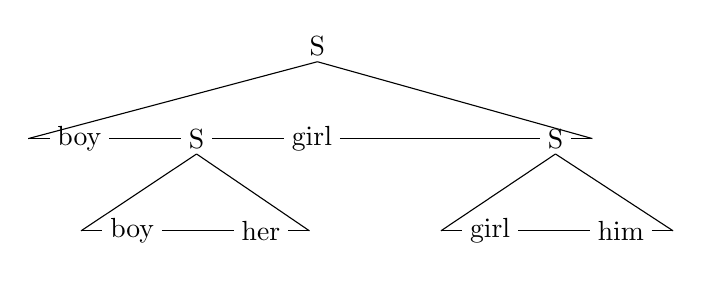
\begin{tikzpicture}
\node at (0.000000, 0.000000) {S};
\node at (-3.023544, -1.171530) {boy};
\node at (-1.534714, -1.171530) {S};
\node at (-2.352594, -2.343060) {boy};
\node at (-0.716835, -2.343060) {her};
\node at (-0.069804, -1.171530) {girl};
\node at (3.023544, -1.171530) {S};
\node at (2.193461, -2.343060) {girl};
\node at (3.853627, -2.343060) {him};
\draw (0.000000,-0.195255) -- (-3.672771,-1.171530);
\draw (0.000000,-0.195255) -- (3.492159,-1.171530);
\draw (-3.672771,-1.171530) -- (-3.401784,-1.171530);
\draw (-2.645304,-1.171530) -- (-1.732342,-1.171530);
\draw (-1.337086,-1.171530) -- (-0.424125,-1.171530);
\draw (0.284517,-1.171530) -- (2.825916,-1.171530);
\draw (3.221172,-1.171530) -- (3.492159,-1.171530);
\draw (-1.534714,-1.366785) -- (-3.001821,-2.343060);
\draw (-1.534714,-1.366785) -- (-0.101290,-2.343060);
\draw (-3.001821,-2.343060) -- (-2.730834,-2.343060);
\draw (-1.974354,-2.343060) -- (-1.061393,-2.343060);
\draw (-0.372277,-2.343060) -- (-0.101290,-2.343060);
\draw (3.023544,-1.366785) -- (1.568152,-2.343060);
\draw (3.023544,-1.366785) -- (4.517499,-2.343060);
\draw (1.568152,-2.343060) -- (1.839139,-2.343060);
\draw (2.547782,-2.343060) -- (3.460743,-2.343060);
\draw (4.246512,-2.343060) -- (4.517499,-2.343060);
\end{tikzpicture}
}
\end{minipage}
\bigbreak

\bigbreak
\begin{minipage}{\textwidth}
  \makebox[\textwidth][c]{
  \begin{tabular}{|r|c|c|c|c|c|c|c|c|c|}
    \hline
    \multicolumn{10}{|c|}{\textbf{Features}} \\
    \hline
    & \textbf{\texttt{PNF}}
    & \textbf{\texttt{FPF}} & \textbf{\texttt{SPF}}
    & \textbf{\texttt{TPF}} & \textbf{\texttt{PLF}}
    & \textbf{\texttt{GNF}} & \textbf{\texttt{ANF}}
    & \textbf{\texttt{RPF}} & \textbf{\texttt{GEN}} \\
    \textbf{\texttt{boy}} & \texttt{-}
    & \texttt{-} & \texttt{-}
    & \texttt{+} & \texttt{-}
    & \texttt{-} & \texttt{+}
    & \texttt{-} & \texttt{-} \\
    \textbf{\texttt{her}} & \texttt{+}
    & \texttt{-} & \texttt{-}
    & \texttt{+} & \texttt{-}
    & \texttt{+} & \texttt{+}
    & \texttt{-} & \texttt{?} \\
    \textbf{\texttt{girl}} & \texttt{-}
    & \texttt{-} & \texttt{-}
    & \texttt{+} & \texttt{-}
    & \texttt{+} & \texttt{+}
    & \texttt{-} & \texttt{-} \\
    \textbf{\texttt{him}} & \texttt{+}
    & \texttt{-} & \texttt{-}
    & \texttt{+} & \texttt{-}
    & \texttt{-} & \texttt{+}
    & \texttt{-} & \texttt{-} \\
    \hline
  \end{tabular}
  }
\end{minipage}
\bigbreak

\bigbreak
\begin{minipage}{\textwidth}
  \makebox[\textwidth][c]{
  \begin{tabular}{|r|l|}
    \hline
    \multicolumn{2}{|c|}{\textbf{Nodes}} \\
    \hline
    ${\textbf{\textrm{1}}_{\phantom{z}}}$ & \texttt{\texttt{(S,~up:0,~dn:2,~lt:0,~rt:0,~th:2,~nu:1)}} \\
    ${\textbf{\textrm{2}}_{\phantom{z}}}$ & \texttt{\texttt{(N,~lit:boy,~ftr:[---+--+--],~up:1,~dn:0,}} \\
    & \texttt{\texttt{~lt:0,~rt:3,~th:3,~np:2,~ch:0,~co:${\textrm{2}_{\textrm{a}}}$,~ec:${\textrm{2}_{\textrm{b}}}$,}} \\
    & \texttt{\texttt{~pr:0,~su:5,~nu:2)}} \\
    ${\textbf{\textrm{2}}_{\textbf{\textrm{a}}}}$ & \texttt{\texttt{(E,~sub:A,~ftr:[---+--+--],~np:2,~ch:0,~co:${\textrm{2}_{\textrm{b}}}$)}} \\
    ${\textbf{\textrm{2}}_{\textbf{\textrm{b}}}}$ & \texttt{\texttt{(E,~sub:B,~ftr:[---+--+--],~np:2,~ch:${\textrm{9}_{\textrm{a}}}$,~co:0)}} \\
    ${\textbf{\textrm{3}}_{\phantom{z}}}$ & \texttt{\texttt{(S,~up:1,~dn:4,~lt:2,~rt:6,~th:4,~nu:3)}} \\
    ${\textbf{\textrm{4}}_{\phantom{z}}}$ & \texttt{\texttt{(N,~lit:boy,~ftr:[---+--+--],~up:3,~dn:0,}} \\
    & \texttt{\texttt{~lt:0,~rt:5,~th:5,~np:4,~ch:0,~co:0,~ec:0,}} \\
    & \texttt{\texttt{~pr:0,~su:0,~nu:4)}} \\
    ${\textbf{\textrm{5}}_{\phantom{z}}}$ & \texttt{\texttt{(N,~lit:her,~ftr:[+--+-++-?],~up:3,~dn:0,}} \\
    & \texttt{\texttt{~lt:4,~rt:0,~th:6,~np:5,~ch:0,~co:${\textrm{5}_{\textrm{a}}}$,~ec:${\textrm{5}_{\textrm{a}}}$,}} \\
    & \texttt{\texttt{~pr:2,~su:6,~nu:5)}} \\
    ${\textbf{\textrm{5}}_{\textbf{\textrm{a}}}}$ & \texttt{\texttt{(E,~sub:A,~ftr:[+--+-++-?],~np:5,~ch:0,~co:0)}} \\
    ${\textbf{\textrm{6}}_{\phantom{z}}}$ & \texttt{\texttt{(N,~lit:girl,~ftr:[---+-++--],~up:1,~dn:0,}} \\
    & \texttt{\texttt{~lt:3,~rt:7,~th:7,~np:6,~ch:0,~co:${\textrm{6}_{\textrm{a}}}$,~ec:${\textrm{6}_{\textrm{b}}}$,}} \\
    & \texttt{\texttt{~pr:5,~su:9,~nu:6)}} \\
    ${\textbf{\textrm{6}}_{\textbf{\textrm{a}}}}$ & \texttt{\texttt{(E,~sub:A,~ftr:[---+-++--],~np:6,~ch:0,~co:${\textrm{6}_{\textrm{b}}}$)}} \\
    ${\textbf{\textrm{6}}_{\textbf{\textrm{b}}}}$ & \texttt{\texttt{(E,~sub:B,~ftr:[---+-++--],~np:6,~ch:${\textrm{5}_{\textrm{a}}}$,~co:0)}} \\
    ${\textbf{\textrm{7}}_{\phantom{z}}}$ & \texttt{\texttt{(S,~up:1,~dn:8,~lt:6,~rt:0,~th:8,~nu:7)}} \\
    ${\textbf{\textrm{8}}_{\phantom{z}}}$ & \texttt{\texttt{(N,~lit:girl,~ftr:[---+-++--],~up:7,~dn:0,}} \\
    & \texttt{\texttt{~lt:0,~rt:9,~th:9,~np:8,~ch:0,~co:0,~ec:0,}} \\
    & \texttt{\texttt{~pr:0,~su:0,~nu:8)}} \\
    ${\textbf{\textrm{9}}_{\phantom{z}}}$ & \texttt{\texttt{(N,~lit:him,~ftr:[+--+--+--],~up:7,~dn:0,}} \\
    & \texttt{\texttt{~lt:8,~rt:0,~th:0,~np:9,~ch:0,~co:${\textrm{9}_{\textrm{a}}}$,~ec:${\textrm{9}_{\textrm{a}}}$,}} \\
    & \texttt{\texttt{~pr:6,~su:0,~nu:9)}} \\
    ${\textbf{\textrm{9}}_{\textbf{\textrm{a}}}}$ & \texttt{\texttt{(E,~sub:A,~ftr:[+--+--+--],~np:9,~ch:0,~co:0)}} \\
    \hline
  \end{tabular}
  }
\end{minipage}
\bigbreak

\bigbreak
\begin{minipage}{\textwidth}
\makebox[\textwidth][c]{
\begin{tikzpicture}[
    every node/.style={align=center},
    dotted line/.style={draw, dotted, thick},
    curved arrow/.style={draw, thick, -{Latex[bend]}},
    ]
\node (S) at (2.801186,0.000000) {S};
\node (boy) at (0.410038,-1.171530) {boy};
\node (her) at (1.999093,-1.171530) {her};
\node (girl) at (3.564228,-1.171530) {girl};
\node (him) at (5.177691,-1.171530) {him};
\draw[dotted line] (S) -- (boy);
\draw[dotted line] (S) -- (him);
\draw[dotted line] (boy) -- (her);
\draw[dotted line] (her) -- (girl);
\draw[dotted line] (girl) -- (him);
\node (boyA) at (0.410038,-2.343060) {${\textrm{boy}_{\textrm{a}}}$};
\node (herA) at (1.999093,-2.343060) {${\textrm{her}_{\textrm{a}}}$};
\node (girlA) at (3.564228,-2.343060) {${\textrm{girl}_{\textrm{a}}}$};
\node (himA) at (5.177691,-2.343060) {${\textrm{him}_{\textrm{a}}}$};
\draw[dotted line] (boy) -- (boyA);
\draw[dotted line] (her) -- (herA);
\draw[dotted line] (girl) -- (girlA);
\draw[dotted line] (him) -- (himA);
\node (boyB) at (0.410038,-3.514590) {${\textrm{boy}_{\textrm{b}}}$};
\node (girlB) at (3.564228,-3.514590) {${\textrm{girl}_{\textrm{b}}}$};
\draw[dotted line] (boyA) -- (boyB);
\draw[dotted line] (girlA) -- (girlB);
\draw[curved arrow] (boyB.north east) to [out=28.62,in=-151.38] (himA.south west);
\draw[curved arrow] (girlB.north west) to [out=121.41,in=-58.59] (herA.south east);
\end{tikzpicture}
}
\end{minipage}
\bigbreak

\bigbreak
\begin{minipage}{\textwidth}
  \makebox[\textwidth][c]{
  \begin{tabular}{|l|l|l|l|}
    \hline
    \multicolumn{4}{|c|}{\textbf{Chaining}} \\
    \hline
    \textbf{\texttt{boy}} & \textbf{\texttt{her}}
    & \textbf{\texttt{girl}} & \textbf{\texttt{him}} \\
    ${\texttt{boy}_{\texttt{a}}}$ & ${\texttt{her}_{\texttt{a}}}$
    & ${\texttt{girl}_{\texttt{a}}}$ & ${\texttt{him}_{\texttt{a}}}$ \\
    ${\texttt{boy}_{\texttt{b}}}$\texttt{\symbol{94}}${\texttt{him}_{\texttt{a}}}$ & 
    & ${\texttt{girl}_{\texttt{b}}}$\texttt{\symbol{94}}${\texttt{her}_{\texttt{a}}}$ &  \\
    \hline
  \end{tabular}
  }
\end{minipage}
\bigbreak

\bigbreak
\begin{minipage}{\textwidth}
  \makebox[\textwidth][c]{
  \begin{tabular}{|c|}
    \hline
    \multicolumn{1}{|c|}{\textbf{Interpretations}} \\
    \hline
    ${\texttt{girl}_{\texttt{b}}}$\texttt{\symbol{94}}${\texttt{her}_{\texttt{a}}}$\qquad ${\texttt{boy}_{\texttt{b}}}$\texttt{\symbol{94}}${\texttt{him}_{\texttt{a}}}$ \\
    \hline
  \end{tabular}
  }
\end{minipage}
\bigbreak

\clearpage

%%%%%%%%%%%%%%%%%%%%%%%%%%%%%%%%%%%%%%%%%%%%%%%%%%%%%%%%%%%%%%%%
%
%     (1.2) *John killed herself.
%
%%%%%%%%%%%%%%%%%%%%%%%%%%%%%%%%%%%%%%%%%%%%%%%%%%%%%%%%%%%%%%%%

\section*{(1.2) *John killed herself.}
\addcontentsline{toc}{section}{(1.2) *John killed herself.}

\bigbreak
\begin{enumerate*}
\item[(1.2)] *John killed herself.
\end{enumerate*}
\bigbreak
\bigbreak
\begin{minipage}{\textwidth}
\makebox[\textwidth][c]{
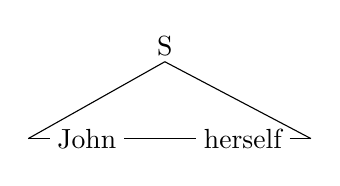
\begin{tikzpicture}
\node at (0.000000, 0.000000) {S};
\node at (-0.990437, -1.171530) {John};
\node at (0.990437, -1.171530) {herself};
\draw (0.000000,-0.195255) -- (-1.734851,-1.171530);
\draw (0.000000,-0.195255) -- (1.855909,-1.171530);
\draw (-1.734851,-1.171530) -- (-1.463864,-1.171530);
\draw (-0.517010,-1.171530) -- (0.395952,-1.171530);
\draw (1.584922,-1.171530) -- (1.855909,-1.171530);
\end{tikzpicture}
}
\end{minipage}
\bigbreak

\bigbreak
\begin{minipage}{\textwidth}
  \makebox[\textwidth][c]{
  \begin{tabular}{|r|c|c|c|c|c|c|c|c|c|}
    \hline
    \multicolumn{10}{|c|}{\textbf{Features}} \\
    \hline
    & \textbf{\texttt{PNF}}
    & \textbf{\texttt{FPF}} & \textbf{\texttt{SPF}}
    & \textbf{\texttt{TPF}} & \textbf{\texttt{PLF}}
    & \textbf{\texttt{GNF}} & \textbf{\texttt{ANF}}
    & \textbf{\texttt{RPF}} & \textbf{\texttt{GEN}} \\
    \textbf{\texttt{John}} & \texttt{-}
    & \texttt{-} & \texttt{-}
    & \texttt{+} & \texttt{-}
    & \texttt{-} & \texttt{+}
    & \texttt{-} & \texttt{-} \\
    \textbf{\texttt{herself}} & \texttt{+}
    & \texttt{-} & \texttt{-}
    & \texttt{+} & \texttt{-}
    & \texttt{+} & \texttt{+}
    & \texttt{+} & \texttt{-} \\
    \hline
  \end{tabular}
  }
\end{minipage}
\bigbreak

\bigbreak
\begin{minipage}{\textwidth}
  \makebox[\textwidth][c]{
  \begin{tabular}{|r|l|}
    \hline
    \multicolumn{2}{|c|}{\textbf{Nodes}} \\
    \hline
    ${\textbf{\textrm{1}}_{\phantom{z}}}$ & \texttt{\texttt{(S,~up:0,~dn:2,~lt:0,~rt:0,~th:2,~nu:1)}} \\
    ${\textbf{\textrm{2}}_{\phantom{z}}}$ & \texttt{\texttt{(N,~lit:John,~ftr:[---+--+--],~up:1,~dn:0,}} \\
    & \texttt{\texttt{~lt:0,~rt:3,~th:3,~np:2,~ch:0,~co:${\textrm{2}_{\textrm{a}}}$,~ec:${\textrm{2}_{\textrm{a}}}$,}} \\
    & \texttt{\texttt{~pr:0,~su:3,~nu:2)}} \\
    ${\textbf{\textrm{2}}_{\textbf{\textrm{a}}}}$ & \texttt{\texttt{(E,~sub:A,~ftr:[---+--+--],~np:2,~ch:0,~co:0)}} \\
    ${\textbf{\textrm{3}}_{\phantom{z}}}$ & \texttt{\texttt{(N,~lit:herself,~ftr:[+--+-+++-],~up:1,~dn:0,}} \\
    & \texttt{\texttt{~lt:2,~rt:0,~th:0,~np:3,~ch:0,~co:${\textrm{3}_{\textrm{a}}}$,~ec:${\textrm{3}_{\textrm{a}}}$,}} \\
    & \texttt{\texttt{~pr:2,~su:0,~nu:3)}} \\
    ${\textbf{\textrm{3}}_{\textbf{\textrm{a}}}}$ & \texttt{\texttt{(E,~sub:A,~ftr:[+--+-+++-],~np:3,~ch:0,~co:0)}} \\
    \hline
  \end{tabular}
  }
\end{minipage}
\bigbreak

\bigbreak
\begin{minipage}{\textwidth}
\makebox[\textwidth][c]{
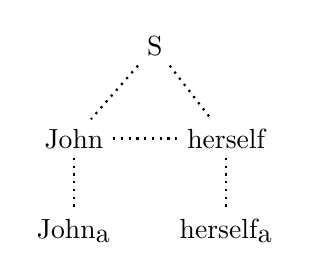
\begin{tikzpicture}[
    every node/.style={align=center},
    dotted line/.style={draw, dotted, thick},
    curved arrow/.style={draw, thick, -{Latex[bend]}},
    ]
\node (S) at (1.532839,0.000000) {S};
\node (John) at (0.505225,-1.171530) {John};
\node (herself) at (2.439394,-1.171530) {herself};
\draw[dotted line] (S) -- (John);
\draw[dotted line] (S) -- (herself);
\draw[dotted line] (John) -- (herself);
\node (JohnA) at (0.505225,-2.343060) {${\textrm{John}_{\textrm{a}}}$};
\node (herselfA) at (2.439394,-2.343060) {${\textrm{herself}_{\textrm{a}}}$};
\draw[dotted line] (John) -- (JohnA);
\draw[dotted line] (herself) -- (herselfA);
\end{tikzpicture}
}
\end{minipage}
\bigbreak

\bigbreak
\begin{minipage}{\textwidth}
  \makebox[\textwidth][c]{
  \begin{tabular}{|l|l|}
    \hline
    \multicolumn{2}{|c|}{\textbf{Chaining}} \\
    \hline
    \textbf{\texttt{John}} & \textbf{\texttt{herself}} \\
    ${\texttt{John}_{\texttt{a}}}$ & ${\texttt{herself}_{\texttt{a}}}$ \\
    \hline
  \end{tabular}
  }
\end{minipage}
\bigbreak

\bigbreak
\begin{minipage}{\textwidth}
  \makebox[\textwidth][c]{
  \begin{tabular}{|c|}
    \hline
    \multicolumn{1}{|c|}{\textbf{Interpretations}} \\
    \hline
    NONE \\
    \hline
  \end{tabular}
  }
\end{minipage}
\bigbreak

\clearpage

%%%%%%%%%%%%%%%%%%%%%%%%%%%%%%%%%%%%%%%%%%%%%%%%%%%%%%%%%%%%%%%%
%
%     (1.4) Some students think they are smarter than they are.
%
%%%%%%%%%%%%%%%%%%%%%%%%%%%%%%%%%%%%%%%%%%%%%%%%%%%%%%%%%%%%%%%%

\section*{(1.4) Some students think they are smarter than they are.}
\addcontentsline{toc}{section}{(1.4) Some students think they are smarter than they are.}

\bigbreak
\begin{enumerate*}
\item[(1.4)] Some students think they are smarter than they are.
\end{enumerate*}
\bigbreak
\bigbreak
\begin{minipage}{\textwidth}
\makebox[\textwidth][c]{
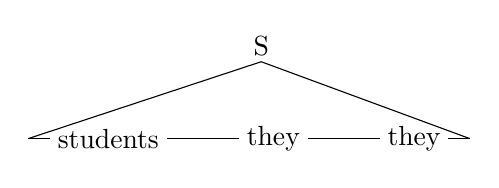
\begin{tikzpicture}
\node at (0.000000, 0.000000) {S};
\node at (-1.941335, -1.171530) {students};
\node at (0.154740, -1.171530) {they};
\node at (1.941335, -1.171530) {they};
\draw (0.000000,-0.195255) -- (-2.958619,-1.171530);
\draw (0.000000,-0.195255) -- (2.649138,-1.171530);
\draw (-2.958619,-1.171530) -- (-2.687631,-1.171530);
\draw (-1.195038,-1.171530) -- (-0.282076,-1.171530);
\draw (0.591557,-1.171530) -- (1.504518,-1.171530);
\draw (2.378151,-1.171530) -- (2.649138,-1.171530);
\end{tikzpicture}
}
\end{minipage}
\bigbreak

\bigbreak
\begin{minipage}{\textwidth}
  \makebox[\textwidth][c]{
  \begin{tabular}{|r|c|c|c|c|c|c|c|c|c|}
    \hline
    \multicolumn{10}{|c|}{\textbf{Features}} \\
    \hline
    & \textbf{\texttt{PNF}}
    & \textbf{\texttt{FPF}} & \textbf{\texttt{SPF}}
    & \textbf{\texttt{TPF}} & \textbf{\texttt{PLF}}
    & \textbf{\texttt{GNF}} & \textbf{\texttt{ANF}}
    & \textbf{\texttt{RPF}} & \textbf{\texttt{GEN}} \\
    \textbf{\texttt{students}} & \texttt{-}
    & \texttt{-} & \texttt{-}
    & \texttt{+} & \texttt{+}
    & \texttt{?} & \texttt{+}
    & \texttt{-} & \texttt{-} \\
    \textbf{\texttt{they}} & \texttt{+}
    & \texttt{-} & \texttt{-}
    & \texttt{+} & \texttt{+}
    & \texttt{?} & \texttt{+}
    & \texttt{-} & \texttt{-} \\
    \hline
  \end{tabular}
  }
\end{minipage}
\bigbreak

\bigbreak
\begin{minipage}{\textwidth}
  \makebox[\textwidth][c]{
  \begin{tabular}{|r|l|}
    \hline
    \multicolumn{2}{|c|}{\textbf{Nodes}} \\
    \hline
    ${\textbf{\textrm{1}}_{\phantom{z}}}$ & \texttt{\texttt{(S,~up:0,~dn:2,~lt:0,~rt:0,~th:2,~nu:1)}} \\
    ${\textbf{\textrm{2}}_{\phantom{z}}}$ & \texttt{\texttt{(N,~lit:students,~ftr:[---++?+--],~up:1,~dn:0,}} \\
    & \texttt{\texttt{~lt:0,~rt:3,~th:3,~np:2,~ch:0,~co:${\textrm{2}_{\textrm{a}}}$,~ec:${\textrm{2}_{\textrm{a}}}$,}} \\
    & \texttt{\texttt{~pr:0,~su:3,~nu:2)}} \\
    ${\textbf{\textrm{2}}_{\textbf{\textrm{a}}}}$ & \texttt{\texttt{(E,~sub:A,~ftr:[---++?+--],~np:2,~ch:0,~co:0)}} \\
    ${\textbf{\textrm{3}}_{\phantom{z}}}$ & \texttt{\texttt{(N,~lit:they,~ftr:[+--++?+--],~up:1,~dn:0,}} \\
    & \texttt{\texttt{~lt:2,~rt:4,~th:4,~np:3,~ch:0,~co:${\textrm{3}_{\textrm{a}}}$,~ec:${\textrm{3}_{\textrm{a}}}$,}} \\
    & \texttt{\texttt{~pr:2,~su:0,~nu:3)}} \\
    ${\textbf{\textrm{3}}_{\textbf{\textrm{a}}}}$ & \texttt{\texttt{(E,~sub:A,~ftr:[+--++?+--],~np:3,~ch:0,~co:0)}} \\
    ${\textbf{\textrm{4}}_{\phantom{z}}}$ & \texttt{\texttt{(N,~lit:they,~ftr:[+--++?+--],~up:1,~dn:0,}} \\
    & \texttt{\texttt{~lt:3,~rt:0,~th:0,~np:4,~ch:0,~co:0,~ec:0,}} \\
    & \texttt{\texttt{~pr:0,~su:0,~nu:4)}} \\
    \hline
  \end{tabular}
  }
\end{minipage}
\bigbreak

\bigbreak
\begin{minipage}{\textwidth}
\makebox[\textwidth][c]{
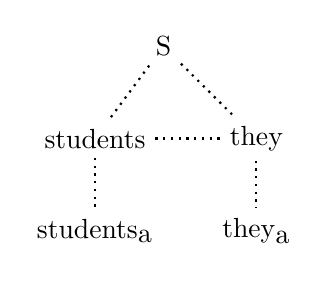
\begin{tikzpicture}[
    every node/.style={align=center},
    dotted line/.style={draw, dotted, thick},
    curved arrow/.style={draw, thick, -{Latex[bend]}},
    ]
\node (S) at (1.648040,0.000000) {S};
\node (students) at (0.778095,-1.171530) {students};
\node (they) at (2.827465,-1.171530) {they};
\draw[dotted line] (S) -- (students);
\draw[dotted line] (S) -- (they);
\draw[dotted line] (students) -- (they);
\node (studentsA) at (0.778095,-2.343060) {${\textrm{students}_{\textrm{a}}}$};
\node (theyA) at (2.827465,-2.343060) {${\textrm{they}_{\textrm{a}}}$};
\draw[dotted line] (students) -- (studentsA);
\draw[dotted line] (they) -- (theyA);
\end{tikzpicture}
}
\end{minipage}
\bigbreak

\bigbreak
\begin{minipage}{\textwidth}
  \makebox[\textwidth][c]{
  \begin{tabular}{|l|l|}
    \hline
    \multicolumn{2}{|c|}{\textbf{Chaining}} \\
    \hline
    \textbf{\texttt{students}} & \textbf{\texttt{they}} \\
    ${\texttt{students}_{\texttt{a}}}$ & ${\texttt{they}_{\texttt{a}}}$ \\
    \hline
  \end{tabular}
  }
\end{minipage}
\bigbreak

\bigbreak
\begin{minipage}{\textwidth}
  \makebox[\textwidth][c]{
  \begin{tabular}{|c|}
    \hline
    \multicolumn{1}{|c|}{\textbf{Interpretations}} \\
    \hline
    NONE \\
    \hline
  \end{tabular}
  }
\end{minipage}
\bigbreak

\clearpage

%%%%%%%%%%%%%%%%%%%%%%%%%%%%%%%%%%%%%%%%%%%%%%%%%%%%%%%%%%%%%%%%
%
%     (1.6) My uncle has never ridden a camel but his brother has, although it was lame.
%
%%%%%%%%%%%%%%%%%%%%%%%%%%%%%%%%%%%%%%%%%%%%%%%%%%%%%%%%%%%%%%%%

\section*{(1.6) My uncle has never ridden a camel but his brother has, although it was lame.}
\addcontentsline{toc}{section}{(1.6) My uncle has never ridden a camel but his brother has, although it was lame.}

\bigbreak
\begin{enumerate*}
\item[(1.6)] My uncle has never ridden a camel but his brother has, although it was lame.
\end{enumerate*}
\bigbreak
\bigbreak
\begin{minipage}{\textwidth}
\makebox[\textwidth][c]{
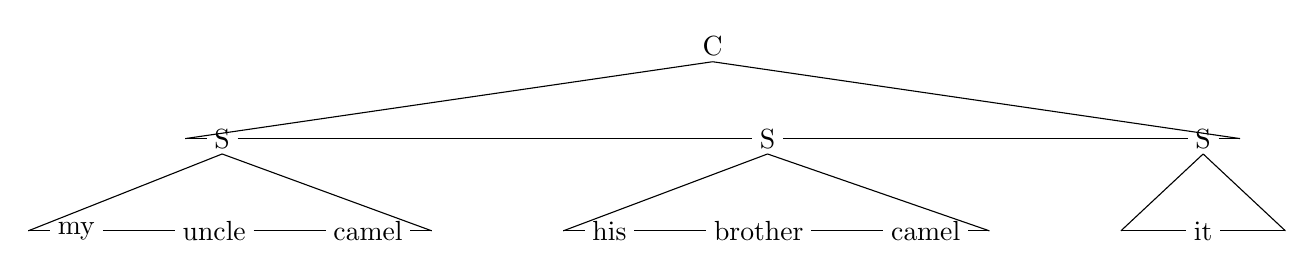
\begin{tikzpicture}
\node at (0.000000, 0.000000) {C};
\node at (-6.229407, -1.171530) {S};
\node at (-8.081900, -2.343060) {my};
\node at (-6.329475, -2.343060) {uncle};
\node at (-4.376913, -2.343060) {camel};
\node at (0.697308, -1.171530) {S};
\node at (-1.310413, -2.343060) {his};
\node at (0.585524, -2.343060) {brother};
\node at (2.705030, -2.343060) {camel};
\node at (6.229407, -1.171530) {S};
\node at (6.229407, -2.343060) {it};
\draw (0.000000,-0.195255) -- (-6.698022,-1.171530);
\draw (0.000000,-0.195255) -- (6.698022,-1.171530);
\draw (-6.698022,-1.171530) -- (-6.427035,-1.171530);
\draw (-6.031778,-1.171530) -- (0.499680,-1.171530);
\draw (0.894936,-1.171530) -- (6.031778,-1.171530);
\draw (6.427035,-1.171530) -- (6.698022,-1.171530);
\draw (-6.229407,-1.366785) -- (-8.692076,-2.343060);
\draw (-6.229407,-1.366785) -- (-3.566600,-2.343060);
\draw (-8.692076,-2.343060) -- (-8.421089,-2.343060);
\draw (-7.742711,-2.343060) -- (-6.829749,-2.343060);
\draw (-5.829201,-2.343060) -- (-4.916239,-2.343060);
\draw (-3.837587,-2.343060) -- (-3.566600,-2.343060);
\draw (0.697308,-1.366785) -- (-1.897158,-2.343060);
\draw (0.697308,-1.366785) -- (3.515343,-2.343060);
\draw (-1.897158,-2.343060) -- (-1.626171,-2.343060);
\draw (-0.994656,-2.343060) -- (-0.081694,-2.343060);
\draw (1.252743,-2.343060) -- (2.165704,-2.343060);
\draw (3.244356,-2.343060) -- (3.515343,-2.343060);
\draw (6.229407,-1.366785) -- (5.184785,-2.343060);
\draw (6.229407,-1.366785) -- (7.274028,-2.343060);
\draw (5.184785,-2.343060) -- (6.012253,-2.343060);
\draw (6.446560,-2.343060) -- (7.274028,-2.343060);
\end{tikzpicture}
}
\end{minipage}
\bigbreak

\bigbreak
\begin{minipage}{\textwidth}
  \makebox[\textwidth][c]{
  \begin{tabular}{|r|c|c|c|c|c|c|c|c|c|}
    \hline
    \multicolumn{10}{|c|}{\textbf{Features}} \\
    \hline
    & \textbf{\texttt{PNF}}
    & \textbf{\texttt{FPF}} & \textbf{\texttt{SPF}}
    & \textbf{\texttt{TPF}} & \textbf{\texttt{PLF}}
    & \textbf{\texttt{GNF}} & \textbf{\texttt{ANF}}
    & \textbf{\texttt{RPF}} & \textbf{\texttt{GEN}} \\
    \textbf{\texttt{my}} & \texttt{+}
    & \texttt{+} & \texttt{-}
    & \texttt{-} & \texttt{-}
    & \texttt{?} & \texttt{+}
    & \texttt{-} & \texttt{+} \\
    \textbf{\texttt{uncle}} & \texttt{-}
    & \texttt{-} & \texttt{-}
    & \texttt{+} & \texttt{-}
    & \texttt{-} & \texttt{+}
    & \texttt{-} & \texttt{-} \\
    \textbf{\texttt{camel}} & \texttt{-}
    & \texttt{-} & \texttt{-}
    & \texttt{+} & \texttt{-}
    & \texttt{?} & \texttt{+}
    & \texttt{-} & \texttt{-} \\
    \textbf{\texttt{his}} & \texttt{+}
    & \texttt{-} & \texttt{-}
    & \texttt{+} & \texttt{-}
    & \texttt{-} & \texttt{+}
    & \texttt{-} & \texttt{+} \\
    \textbf{\texttt{brother}} & \texttt{-}
    & \texttt{-} & \texttt{-}
    & \texttt{+} & \texttt{-}
    & \texttt{-} & \texttt{+}
    & \texttt{-} & \texttt{-} \\
    \textbf{\texttt{it}} & \texttt{+}
    & \texttt{-} & \texttt{-}
    & \texttt{+} & \texttt{-}
    & \texttt{?} & \texttt{-}
    & \texttt{-} & \texttt{-} \\
    \hline
  \end{tabular}
  }
\end{minipage}
\bigbreak

\bigbreak
\begin{minipage}{\textwidth}
  \makebox[\textwidth][c]{
  \begin{tabular}{|r|l|}
    \hline
    \multicolumn{2}{|c|}{\textbf{Nodes}} \\
    \hline
    ${\textbf{\textrm{1}}_{\phantom{z}}}$ & \texttt{\texttt{(C,~up:0,~dn:2,~lt:0,~rt:0,~th:2,~nu:1)}} \\
    ${\textbf{\textrm{2}}_{\phantom{z}}}$ & \texttt{\texttt{(S,~up:1,~dn:3,~lt:0,~rt:6,~th:3,~nu:2)}} \\
    ${\textbf{\textrm{3}}_{\phantom{z}}}$ & \texttt{\texttt{(N,~lit:my,~ftr:[++---?+-+],~up:2,~dn:0,}} \\
    & \texttt{\texttt{~lt:0,~rt:4,~th:4,~np:3,~ch:0,~co:${\textrm{3}_{\textrm{a}}}$,~ec:${\textrm{3}_{\textrm{a}}}$,}} \\
    & \texttt{\texttt{~pr:0,~su:4,~nu:3)}} \\
    ${\textbf{\textrm{3}}_{\textbf{\textrm{a}}}}$ & \texttt{\texttt{(E,~sub:A,~ftr:[++---?+-+],~np:3,~ch:0,~co:0)}} \\
    ${\textbf{\textrm{4}}_{\phantom{z}}}$ & \texttt{\texttt{(N,~lit:uncle,~ftr:[---+--+--],~up:2,~dn:0,}} \\
    & \texttt{\texttt{~lt:3,~rt:5,~th:5,~np:4,~ch:0,~co:${\textrm{4}_{\textrm{a}}}$,~ec:${\textrm{4}_{\textrm{b}}}$,}} \\
    & \texttt{\texttt{~pr:3,~su:5,~nu:4)}} \\
    ${\textbf{\textrm{4}}_{\textbf{\textrm{a}}}}$ & \texttt{\texttt{(E,~sub:A,~ftr:[---+--+--],~np:4,~ch:0,~co:${\textrm{4}_{\textrm{b}}}$)}} \\
    ${\textbf{\textrm{4}}_{\textbf{\textrm{b}}}}$ & \texttt{\texttt{(E,~sub:B,~ftr:[---+--+--],~np:4,~ch:${\textrm{7}_{\textrm{a}}}$,~co:0)}} \\
    ${\textbf{\textrm{5}}_{\phantom{z}}}$ & \texttt{\texttt{(N,~lit:camel,~ftr:[---+-?+--],~up:2,~dn:0,}} \\
    & \texttt{\texttt{~lt:4,~rt:0,~th:6,~np:5,~ch:0,~co:${\textrm{5}_{\textrm{a}}}$,~ec:${\textrm{5}_{\textrm{b}}}$,}} \\
    & \texttt{\texttt{~pr:4,~su:7,~nu:5)}} \\
    ${\textbf{\textrm{5}}_{\textbf{\textrm{a}}}}$ & \texttt{\texttt{(E,~sub:A,~ftr:[---+-?+--],~np:5,~ch:0,~co:${\textrm{5}_{\textrm{b}}}$)}} \\
    ${\textbf{\textrm{5}}_{\textbf{\textrm{b}}}}$ & \texttt{\texttt{(E,~sub:B,~ftr:[---+--+--],~np:5,~ch:${\textrm{7}_{\textrm{a}}}$,~co:0)}} \\
    ${\textbf{\textrm{6}}_{\phantom{z}}}$ & \texttt{\texttt{(S,~up:1,~dn:7,~lt:2,~rt:10,~th:7,~nu:6)}} \\
    ${\textbf{\textrm{7}}_{\phantom{z}}}$ & \texttt{\texttt{(N,~lit:his,~ftr:[+--+--+-+],~up:6,~dn:0,}} \\
    & \texttt{\texttt{~lt:0,~rt:8,~th:8,~np:7,~ch:0,~co:${\textrm{7}_{\textrm{a}}}$,~ec:${\textrm{7}_{\textrm{a}}}$,}} \\
    & \texttt{\texttt{~pr:5,~su:8,~nu:7)}} \\
    ${\textbf{\textrm{7}}_{\textbf{\textrm{a}}}}$ & \texttt{\texttt{(E,~sub:A,~ftr:[+--+--+-+],~np:7,~ch:0,~co:0)}} \\
    ${\textbf{\textrm{8}}_{\phantom{z}}}$ & \texttt{\texttt{(N,~lit:brother,~ftr:[---+--+--],~up:6,~dn:0,}} \\
    & \texttt{\texttt{~lt:7,~rt:9,~th:9,~np:8,~ch:0,~co:${\textrm{8}_{\textrm{a}}}$,~ec:${\textrm{8}_{\textrm{a}}}$,}} \\
    & \texttt{\texttt{~pr:7,~su:11,~nu:8)}} \\
    ${\textbf{\textrm{8}}_{\textbf{\textrm{a}}}}$ & \texttt{\texttt{(E,~sub:A,~ftr:[---+--+--],~np:8,~ch:0,~co:0)}} \\
    ${\textbf{\textrm{9}}_{\phantom{z}}}$ & \texttt{\texttt{(N,~lit:camel,~ftr:[---+-?+--],~up:6,~dn:0,}} \\
    & \texttt{\texttt{~lt:8,~rt:0,~th:10,~np:9,~ch:0,~co:0,~ec:0,}} \\
    & \texttt{\texttt{~pr:0,~su:0,~nu:9)}} \\
    ${\textbf{\textrm{10}}_{\phantom{z}}}$ & \texttt{\texttt{(S,~up:1,~dn:11,~lt:6,~rt:0,~th:11,~nu:10)}} \\
    ${\textbf{\textrm{11}}_{\phantom{z}}}$ & \texttt{\texttt{(N,~lit:it,~ftr:[+--+-?---],~up:10,~dn:0,}} \\
    & \texttt{\texttt{~lt:0,~rt:0,~th:0,~np:11,~ch:0,~co:${\textrm{11}_{\textrm{a}}}$,~ec:${\textrm{11}_{\textrm{a}}}$,}} \\
    & \texttt{\texttt{~pr:8,~su:0,~nu:11)}} \\
    ${\textbf{\textrm{11}}_{\textbf{\textrm{a}}}}$ & \texttt{\texttt{(E,~sub:A,~ftr:[+--+-?---],~np:11,~ch:0,~co:0)}} \\
    \hline
  \end{tabular}
  }
\end{minipage}
\bigbreak

\bigbreak
\begin{minipage}{\textwidth}
\makebox[\textwidth][c]{
\begin{tikzpicture}[
    every node/.style={align=center},
    dotted line/.style={draw, dotted, thick},
    curved arrow/.style={draw, thick, -{Latex[bend]}},
    ]
\node (S) at (4.776359,0.000000) {S};
\node (my) at (0.370987,-1.171530) {my};
\node (uncle) at (2.076707,-1.171530) {uncle};
\node (camel) at (3.982564,-1.171530) {camel};
\node (his) at (5.703904,-1.171530) {his};
\node (brother) at (7.553137,-1.171530) {brother};
\node (it) at (9.303766,-1.171530) {it};
\draw[dotted line] (S) -- (my);
\draw[dotted line] (S) -- (it);
\draw[dotted line] (my) -- (uncle);
\draw[dotted line] (uncle) -- (camel);
\draw[dotted line] (camel) -- (his);
\draw[dotted line] (his) -- (brother);
\draw[dotted line] (brother) -- (it);
\node (myA) at (0.370987,-2.343060) {${\textrm{my}_{\textrm{a}}}$};
\node (uncleA) at (2.076707,-2.343060) {${\textrm{uncle}_{\textrm{a}}}$};
\node (camelA) at (3.982564,-2.343060) {${\textrm{camel}_{\textrm{a}}}$};
\node (hisA) at (5.703904,-2.343060) {${\textrm{his}_{\textrm{a}}}$};
\node (brotherA) at (7.553137,-2.343060) {${\textrm{brother}_{\textrm{a}}}$};
\node (itA) at (9.303766,-2.343060) {${\textrm{it}_{\textrm{a}}}$};
\draw[dotted line] (my) -- (myA);
\draw[dotted line] (uncle) -- (uncleA);
\draw[dotted line] (camel) -- (camelA);
\draw[dotted line] (his) -- (hisA);
\draw[dotted line] (brother) -- (brotherA);
\draw[dotted line] (it) -- (itA);
\node (uncleB) at (2.076707,-3.514590) {${\textrm{uncle}_{\textrm{b}}}$};
\node (camelB) at (3.982564,-3.514590) {${\textrm{camel}_{\textrm{b}}}$};
\draw[dotted line] (uncleA) -- (uncleB);
\draw[dotted line] (camelA) -- (camelB);
\draw[curved arrow] (camelB.north east) to [out=58.59,in=-81.23] (hisA.south);
\draw[curved arrow] (uncleB.north east) to [out=39.31,in=179.13] (hisA.west);
\end{tikzpicture}
}
\end{minipage}
\bigbreak

\bigbreak
\begin{minipage}{\textwidth}
  \makebox[\textwidth][c]{
  \begin{tabular}{|l|l|l|l|l|l|}
    \hline
    \multicolumn{6}{|c|}{\textbf{Chaining}} \\
    \hline
    \textbf{\texttt{my}} & \textbf{\texttt{uncle}}
    & \textbf{\texttt{camel}} & \textbf{\texttt{his}}
    & \textbf{\texttt{brother}} & \textbf{\texttt{it}} \\
    ${\texttt{my}_{\texttt{a}}}$ & ${\texttt{uncle}_{\texttt{a}}}$
    & ${\texttt{camel}_{\texttt{a}}}$ & ${\texttt{his}_{\texttt{a}}}$
    & ${\texttt{brother}_{\texttt{a}}}$ & ${\texttt{it}_{\texttt{a}}}$ \\
     & ${\texttt{uncle}_{\texttt{b}}}$\texttt{\symbol{94}}${\texttt{his}_{\texttt{a}}}$
    & ${\texttt{camel}_{\texttt{b}}}$\texttt{\symbol{94}}${\texttt{his}_{\texttt{a}}}$ & 
    &  &  \\
    \hline
  \end{tabular}
  }
\end{minipage}
\bigbreak

\bigbreak
\begin{minipage}{\textwidth}
  \makebox[\textwidth][c]{
  \begin{tabular}{|c|}
    \hline
    \multicolumn{1}{|c|}{\textbf{Interpretations}} \\
    \hline
    NONE \\
    \hline
  \end{tabular}
  }
\end{minipage}
\bigbreak

\clearpage

%%%%%%%%%%%%%%%%%%%%%%%%%%%%%%%%%%%%%%%%%%%%%%%%%%%%%%%%%%%%%%%%
%
%     (1.10) I like the fresh candy better than the stale PHI.
%
%%%%%%%%%%%%%%%%%%%%%%%%%%%%%%%%%%%%%%%%%%%%%%%%%%%%%%%%%%%%%%%%

\section*{(1.10) I like the fresh candy better than the stale PHI.}
\addcontentsline{toc}{section}{(1.10) I like the fresh candy better than the stale PHI.}

\bigbreak
\begin{enumerate*}
\item[(1.10)] I like the fresh candy better than the stale PHI.
\end{enumerate*}
\bigbreak
\bigbreak
\begin{minipage}{\textwidth}
\makebox[\textwidth][c]{
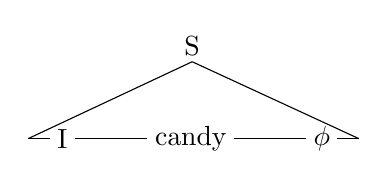
\begin{tikzpicture}
\node at (0.000000, 0.000000) {S};
\node at (-1.647475, -1.171530) {I};
\node at (-0.017085, -1.171530) {candy};
\node at (1.647475, -1.171530) {$\phi$};
\draw (0.000000,-0.195255) -- (-2.081920,-1.171530);
\draw (0.000000,-0.195255) -- (2.116090,-1.171530);
\draw (-2.081920,-1.171530) -- (-1.810933,-1.171530);
\draw (-1.484017,-1.171530) -- (-0.571055,-1.171530);
\draw (0.536885,-1.171530) -- (1.449847,-1.171530);
\draw (1.845103,-1.171530) -- (2.116090,-1.171530);
\end{tikzpicture}
}
\end{minipage}
\bigbreak

\bigbreak
\begin{minipage}{\textwidth}
  \makebox[\textwidth][c]{
  \begin{tabular}{|r|c|c|c|c|c|c|c|c|c|}
    \hline
    \multicolumn{10}{|c|}{\textbf{Features}} \\
    \hline
    & \textbf{\texttt{PNF}}
    & \textbf{\texttt{FPF}} & \textbf{\texttt{SPF}}
    & \textbf{\texttt{TPF}} & \textbf{\texttt{PLF}}
    & \textbf{\texttt{GNF}} & \textbf{\texttt{ANF}}
    & \textbf{\texttt{RPF}} & \textbf{\texttt{GEN}} \\
    \textbf{\texttt{I}} & \texttt{+}
    & \texttt{+} & \texttt{-}
    & \texttt{-} & \texttt{-}
    & \texttt{?} & \texttt{+}
    & \texttt{-} & \texttt{-} \\
    \textbf{\texttt{candy}} & \texttt{-}
    & \texttt{-} & \texttt{-}
    & \texttt{+} & \texttt{-}
    & \texttt{?} & \texttt{-}
    & \texttt{-} & \texttt{-} \\
    $\bm{\phi}$ & \texttt{+}
    & \texttt{?} & \texttt{?}
    & \texttt{?} & \texttt{?}
    & \texttt{?} & \texttt{?}
    & \texttt{-} & \texttt{-} \\
    \hline
  \end{tabular}
  }
\end{minipage}
\bigbreak

\bigbreak
\begin{minipage}{\textwidth}
  \makebox[\textwidth][c]{
  \begin{tabular}{|r|l|}
    \hline
    \multicolumn{2}{|c|}{\textbf{Nodes}} \\
    \hline
    ${\textbf{\textrm{1}}_{\phantom{z}}}$ & \texttt{\texttt{(S,~up:0,~dn:2,~lt:0,~rt:0,~th:2,~nu:1)}} \\
    ${\textbf{\textrm{2}}_{\phantom{z}}}$ & \texttt{\texttt{(N,~lit:I,~ftr:[++---?+--],~up:1,~dn:0,}} \\
    & \texttt{\texttt{~lt:0,~rt:3,~th:3,~np:2,~ch:0,~co:${\textrm{2}_{\textrm{a}}}$,~ec:${\textrm{2}_{\textrm{a}}}$,}} \\
    & \texttt{\texttt{~pr:0,~su:3,~nu:2)}} \\
    ${\textbf{\textrm{2}}_{\textbf{\textrm{a}}}}$ & \texttt{\texttt{(E,~sub:A,~ftr:[++---?+--],~np:2,~ch:0,~co:0)}} \\
    ${\textbf{\textrm{3}}_{\phantom{z}}}$ & \texttt{\texttt{(N,~lit:candy,~ftr:[---+-?---],~up:1,~dn:0,}} \\
    & \texttt{\texttt{~lt:2,~rt:4,~th:4,~np:3,~ch:0,~co:${\textrm{3}_{\textrm{a}}}$,~ec:${\textrm{3}_{\textrm{a}}}$,}} \\
    & \texttt{\texttt{~pr:2,~su:4,~nu:3)}} \\
    ${\textbf{\textrm{3}}_{\textbf{\textrm{a}}}}$ & \texttt{\texttt{(E,~sub:A,~ftr:[---+-?---],~np:3,~ch:0,~co:0)}} \\
    ${\textbf{\textrm{4}}_{\phantom{z}}}$ & \texttt{\texttt{(N,~lit:$\phi$,~ftr:[+??????--],~up:1,~dn:0,}} \\
    & \texttt{\texttt{~lt:3,~rt:0,~th:0,~np:4,~ch:0,~co:${\textrm{4}_{\textrm{a}}}$,~ec:${\textrm{4}_{\textrm{a}}}$,}} \\
    & \texttt{\texttt{~pr:3,~su:0,~nu:4)}} \\
    ${\textbf{\textrm{4}}_{\textbf{\textrm{a}}}}$ & \texttt{\texttt{(E,~sub:A,~ftr:[+??????--],~np:4,~ch:0,~co:0)}} \\
    \hline
  \end{tabular}
  }
\end{minipage}
\bigbreak

\bigbreak
\begin{minipage}{\textwidth}
\makebox[\textwidth][c]{
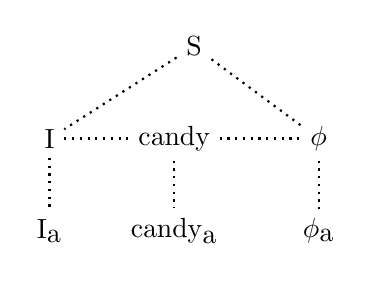
\begin{tikzpicture}[
    every node/.style={align=center},
    dotted line/.style={draw, dotted, thick},
    curved arrow/.style={draw, thick, -{Latex[bend]}},
    ]
\node (S) at (2.030333,0.000000) {S};
\node (I) at (0.195256,-1.171530) {I};
\node (candy) at (1.778941,-1.171530) {candy};
\node (PHI) at (3.614018,-1.171530) {$\phi$};
\draw[dotted line] (S) -- (I);
\draw[dotted line] (S) -- (PHI);
\draw[dotted line] (I) -- (candy);
\draw[dotted line] (candy) -- (PHI);
\node (IA) at (0.195256,-2.343060) {${\textrm{I}_{\textrm{a}}}$};
\node (candyA) at (1.778941,-2.343060) {${\textrm{candy}_{\textrm{a}}}$};
\node (PHIA) at (3.614018,-2.343060) {${\phi_{\textrm{a}}}$};
\draw[dotted line] (I) -- (IA);
\draw[dotted line] (candy) -- (candyA);
\draw[dotted line] (PHI) -- (PHIA);
\end{tikzpicture}
}
\end{minipage}
\bigbreak

\bigbreak
\begin{minipage}{\textwidth}
  \makebox[\textwidth][c]{
  \begin{tabular}{|l|l|l|}
    \hline
    \multicolumn{3}{|c|}{\textbf{Chaining}} \\
    \hline
    \textbf{\texttt{I}} & \textbf{\texttt{candy}}
    & $\bm{\phi}$ \\
    ${\texttt{I}_{\texttt{a}}}$ & ${\texttt{candy}_{\texttt{a}}}$
    & ${\phi_{\texttt{a}}}$ \\
    \hline
  \end{tabular}
  }
\end{minipage}
\bigbreak

\bigbreak
\begin{minipage}{\textwidth}
  \makebox[\textwidth][c]{
  \begin{tabular}{|c|}
    \hline
    \multicolumn{1}{|c|}{\textbf{Interpretations}} \\
    \hline
    NONE \\
    \hline
  \end{tabular}
  }
\end{minipage}
\bigbreak

\clearpage

%%%%%%%%%%%%%%%%%%%%%%%%%%%%%%%%%%%%%%%%%%%%%%%%%%%%%%%%%%%%%%%%
%
%     (1.11) If John can, he will do it.
%
%%%%%%%%%%%%%%%%%%%%%%%%%%%%%%%%%%%%%%%%%%%%%%%%%%%%%%%%%%%%%%%%

\section*{(1.11) If John can, he will do it.}
\addcontentsline{toc}{section}{(1.11) If John can, he will do it.}

\bigbreak
\begin{enumerate*}
\item[(1.11)] If John can, he will do it.
\end{enumerate*}
\bigbreak
\bigbreak
\begin{minipage}{\textwidth}
\makebox[\textwidth][c]{
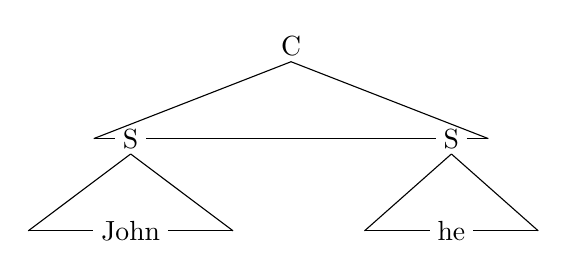
\begin{tikzpicture}
\node at (0.000000, 0.000000) {C};
\node at (-2.036768, -1.171530) {S};
\node at (-2.036768, -2.343060) {John};
\node at (2.036768, -1.171530) {S};
\node at (2.036768, -2.343060) {he};
\draw (0.000000,-0.195255) -- (-2.505383,-1.171530);
\draw (0.000000,-0.195255) -- (2.505383,-1.171530);
\draw (-2.505383,-1.171530) -- (-2.234396,-1.171530);
\draw (-1.839140,-1.171530) -- (1.839140,-1.171530);
\draw (2.234396,-1.171530) -- (2.505383,-1.171530);
\draw (-2.036768,-1.366785) -- (-3.337663,-2.343060);
\draw (-2.036768,-1.366785) -- (-0.735872,-2.343060);
\draw (-3.337663,-2.343060) -- (-2.510195,-2.343060);
\draw (-1.563340,-2.343060) -- (-0.735872,-2.343060);
\draw (2.036768,-1.366785) -- (0.933570,-2.343060);
\draw (2.036768,-1.366785) -- (3.139966,-2.343060);
\draw (0.933570,-2.343060) -- (1.761037,-2.343060);
\draw (2.312498,-2.343060) -- (3.139966,-2.343060);
\end{tikzpicture}
}
\end{minipage}
\bigbreak

\bigbreak
\begin{minipage}{\textwidth}
  \makebox[\textwidth][c]{
  \begin{tabular}{|r|c|c|c|c|c|c|c|c|c|}
    \hline
    \multicolumn{10}{|c|}{\textbf{Features}} \\
    \hline
    & \textbf{\texttt{PNF}}
    & \textbf{\texttt{FPF}} & \textbf{\texttt{SPF}}
    & \textbf{\texttt{TPF}} & \textbf{\texttt{PLF}}
    & \textbf{\texttt{GNF}} & \textbf{\texttt{ANF}}
    & \textbf{\texttt{RPF}} & \textbf{\texttt{GEN}} \\
    \textbf{\texttt{John}} & \texttt{-}
    & \texttt{-} & \texttt{-}
    & \texttt{+} & \texttt{-}
    & \texttt{-} & \texttt{+}
    & \texttt{-} & \texttt{-} \\
    \textbf{\texttt{he}} & \texttt{+}
    & \texttt{-} & \texttt{-}
    & \texttt{+} & \texttt{-}
    & \texttt{-} & \texttt{+}
    & \texttt{-} & \texttt{-} \\
    \hline
  \end{tabular}
  }
\end{minipage}
\bigbreak

\bigbreak
\begin{minipage}{\textwidth}
  \makebox[\textwidth][c]{
  \begin{tabular}{|r|l|}
    \hline
    \multicolumn{2}{|c|}{\textbf{Nodes}} \\
    \hline
    ${\textbf{\textrm{1}}_{\phantom{z}}}$ & \texttt{\texttt{(C,~up:0,~dn:2,~lt:0,~rt:0,~th:2,~nu:1)}} \\
    ${\textbf{\textrm{2}}_{\phantom{z}}}$ & \texttt{\texttt{(S,~up:1,~dn:3,~lt:0,~rt:4,~th:3,~nu:2)}} \\
    ${\textbf{\textrm{3}}_{\phantom{z}}}$ & \texttt{\texttt{(N,~lit:John,~ftr:[---+--+--],~up:2,~dn:0,}} \\
    & \texttt{\texttt{~lt:0,~rt:0,~th:4,~np:3,~ch:0,~co:${\textrm{3}_{\textrm{a}}}$,~ec:${\textrm{3}_{\textrm{b}}}$,}} \\
    & \texttt{\texttt{~pr:0,~su:5,~nu:3)}} \\
    ${\textbf{\textrm{3}}_{\textbf{\textrm{a}}}}$ & \texttt{\texttt{(E,~sub:A,~ftr:[---+--+--],~np:3,~ch:0,~co:${\textrm{3}_{\textrm{b}}}$)}} \\
    ${\textbf{\textrm{3}}_{\textbf{\textrm{b}}}}$ & \texttt{\texttt{(E,~sub:B,~ftr:[---+--+--],~np:3,~ch:${\textrm{5}_{\textrm{a}}}$,~co:0)}} \\
    ${\textbf{\textrm{4}}_{\phantom{z}}}$ & \texttt{\texttt{(S,~up:1,~dn:5,~lt:2,~rt:0,~th:5,~nu:4)}} \\
    ${\textbf{\textrm{5}}_{\phantom{z}}}$ & \texttt{\texttt{(N,~lit:he,~ftr:[+--+--+--],~up:4,~dn:0,}} \\
    & \texttt{\texttt{~lt:0,~rt:0,~th:0,~np:5,~ch:0,~co:${\textrm{5}_{\textrm{a}}}$,~ec:${\textrm{5}_{\textrm{a}}}$,}} \\
    & \texttt{\texttt{~pr:3,~su:0,~nu:5)}} \\
    ${\textbf{\textrm{5}}_{\textbf{\textrm{a}}}}$ & \texttt{\texttt{(E,~sub:A,~ftr:[+--+--+--],~np:5,~ch:0,~co:0)}} \\
    \hline
  \end{tabular}
  }
\end{minipage}
\bigbreak

\bigbreak
\begin{minipage}{\textwidth}
\makebox[\textwidth][c]{
\begin{tikzpicture}[
    every node/.style={align=center},
    dotted line/.style={draw, dotted, thick},
    curved arrow/.style={draw, thick, -{Latex[bend]}},
    ]
\node (S) at (1.214084,0.000000) {S};
\node (John) at (0.505225,-1.171530) {John};
\node (he) at (2.120639,-1.171530) {he};
\draw[dotted line] (S) -- (John);
\draw[dotted line] (S) -- (he);
\draw[dotted line] (John) -- (he);
\node (JohnA) at (0.505225,-2.343060) {${\textrm{John}_{\textrm{a}}}$};
\node (heA) at (2.120639,-2.343060) {${\textrm{he}_{\textrm{a}}}$};
\draw[dotted line] (John) -- (JohnA);
\draw[dotted line] (he) -- (heA);
\node (JohnB) at (0.505225,-3.514590) {${\textrm{John}_{\textrm{b}}}$};
\draw[dotted line] (JohnA) -- (JohnB);
\draw[curved arrow] (JohnB.north east) to [out=58.59,in=-121.41] (heA.south west);
\end{tikzpicture}
}
\end{minipage}
\bigbreak

\bigbreak
\begin{minipage}{\textwidth}
  \makebox[\textwidth][c]{
  \begin{tabular}{|l|l|}
    \hline
    \multicolumn{2}{|c|}{\textbf{Chaining}} \\
    \hline
    \textbf{\texttt{John}} & \textbf{\texttt{he}} \\
    ${\texttt{John}_{\texttt{a}}}$ & ${\texttt{he}_{\texttt{a}}}$ \\
    ${\texttt{John}_{\texttt{b}}}$\texttt{\symbol{94}}${\texttt{he}_{\texttt{a}}}$ &  \\
    \hline
  \end{tabular}
  }
\end{minipage}
\bigbreak

\bigbreak
\begin{minipage}{\textwidth}
  \makebox[\textwidth][c]{
  \begin{tabular}{|c|}
    \hline
    \multicolumn{1}{|c|}{\textbf{Interpretations}} \\
    \hline
    ${\texttt{John}_{\texttt{b}}}$\texttt{\symbol{94}}${\texttt{he}_{\texttt{a}}}$ \\
    \hline
  \end{tabular}
  }
\end{minipage}
\bigbreak

\clearpage

%%%%%%%%%%%%%%%%%%%%%%%%%%%%%%%%%%%%%%%%%%%%%%%%%%%%%%%%%%%%%%%%
%
%     (1.12) If he can, John will do it.
%
%%%%%%%%%%%%%%%%%%%%%%%%%%%%%%%%%%%%%%%%%%%%%%%%%%%%%%%%%%%%%%%%

\section*{(1.12) If he can, John will do it.}
\addcontentsline{toc}{section}{(1.12) If he can, John will do it.}

\bigbreak
\begin{enumerate*}
\item[(1.12)] If he can, John will do it.
\end{enumerate*}
\bigbreak
\bigbreak
\begin{minipage}{\textwidth}
\makebox[\textwidth][c]{
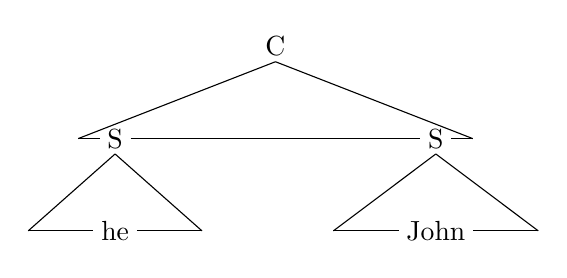
\begin{tikzpicture}
\node at (0.000000, 0.000000) {C};
\node at (-2.036768, -1.171530) {S};
\node at (-2.036768, -2.343060) {he};
\node at (2.036768, -1.171530) {S};
\node at (2.036768, -2.343060) {John};
\draw (0.000000,-0.195255) -- (-2.505383,-1.171530);
\draw (0.000000,-0.195255) -- (2.505383,-1.171530);
\draw (-2.505383,-1.171530) -- (-2.234396,-1.171530);
\draw (-1.839140,-1.171530) -- (1.839140,-1.171530);
\draw (2.234396,-1.171530) -- (2.505383,-1.171530);
\draw (-2.036768,-1.366785) -- (-3.139966,-2.343060);
\draw (-2.036768,-1.366785) -- (-0.933570,-2.343060);
\draw (-3.139966,-2.343060) -- (-2.312498,-2.343060);
\draw (-1.761037,-2.343060) -- (-0.933570,-2.343060);
\draw (2.036768,-1.366785) -- (0.735872,-2.343060);
\draw (2.036768,-1.366785) -- (3.337663,-2.343060);
\draw (0.735872,-2.343060) -- (1.563340,-2.343060);
\draw (2.510195,-2.343060) -- (3.337663,-2.343060);
\end{tikzpicture}
}
\end{minipage}
\bigbreak

\bigbreak
\begin{minipage}{\textwidth}
  \makebox[\textwidth][c]{
  \begin{tabular}{|r|c|c|c|c|c|c|c|c|c|}
    \hline
    \multicolumn{10}{|c|}{\textbf{Features}} \\
    \hline
    & \textbf{\texttt{PNF}}
    & \textbf{\texttt{FPF}} & \textbf{\texttt{SPF}}
    & \textbf{\texttt{TPF}} & \textbf{\texttt{PLF}}
    & \textbf{\texttt{GNF}} & \textbf{\texttt{ANF}}
    & \textbf{\texttt{RPF}} & \textbf{\texttt{GEN}} \\
    \textbf{\texttt{he}} & \texttt{+}
    & \texttt{-} & \texttt{-}
    & \texttt{+} & \texttt{-}
    & \texttt{-} & \texttt{+}
    & \texttt{-} & \texttt{-} \\
    \textbf{\texttt{John}} & \texttt{-}
    & \texttt{-} & \texttt{-}
    & \texttt{+} & \texttt{-}
    & \texttt{-} & \texttt{+}
    & \texttt{-} & \texttt{-} \\
    \hline
  \end{tabular}
  }
\end{minipage}
\bigbreak

\bigbreak
\begin{minipage}{\textwidth}
  \makebox[\textwidth][c]{
  \begin{tabular}{|r|l|}
    \hline
    \multicolumn{2}{|c|}{\textbf{Nodes}} \\
    \hline
    ${\textbf{\textrm{1}}_{\phantom{z}}}$ & \texttt{\texttt{(C,~up:0,~dn:2,~lt:0,~rt:0,~th:2,~nu:1)}} \\
    ${\textbf{\textrm{2}}_{\phantom{z}}}$ & \texttt{\texttt{(S,~up:1,~dn:3,~lt:0,~rt:4,~th:3,~nu:2)}} \\
    ${\textbf{\textrm{3}}_{\phantom{z}}}$ & \texttt{\texttt{(N,~lit:he,~ftr:[+--+--+--],~up:2,~dn:0,}} \\
    & \texttt{\texttt{~lt:0,~rt:0,~th:4,~np:3,~ch:0,~co:${\textrm{3}_{\textrm{a}}}$,~ec:${\textrm{3}_{\textrm{a}}}$,}} \\
    & \texttt{\texttt{~pr:0,~su:5,~nu:3)}} \\
    ${\textbf{\textrm{3}}_{\textbf{\textrm{a}}}}$ & \texttt{\texttt{(E,~sub:A,~ftr:[+--+--+--],~np:3,~ch:0,~co:0)}} \\
    ${\textbf{\textrm{4}}_{\phantom{z}}}$ & \texttt{\texttt{(S,~up:1,~dn:5,~lt:2,~rt:0,~th:5,~nu:4)}} \\
    ${\textbf{\textrm{5}}_{\phantom{z}}}$ & \texttt{\texttt{(N,~lit:John,~ftr:[---+--+--],~up:4,~dn:0,}} \\
    & \texttt{\texttt{~lt:0,~rt:0,~th:0,~np:5,~ch:0,~co:${\textrm{5}_{\textrm{a}}}$,~ec:${\textrm{5}_{\textrm{a}}}$,}} \\
    & \texttt{\texttt{~pr:3,~su:0,~nu:5)}} \\
    ${\textbf{\textrm{5}}_{\textbf{\textrm{a}}}}$ & \texttt{\texttt{(E,~sub:A,~ftr:[---+--+--],~np:5,~ch:0,~co:0)}} \\
    \hline
  \end{tabular}
  }
\end{minipage}
\bigbreak

\bigbreak
\begin{minipage}{\textwidth}
\makebox[\textwidth][c]{
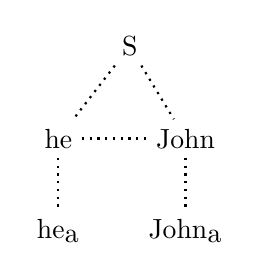
\begin{tikzpicture}[
    every node/.style={align=center},
    dotted line/.style={draw, dotted, thick},
    curved arrow/.style={draw, thick, -{Latex[bend]}},
    ]
\node (S) at (1.214084,0.000000) {S};
\node (he) at (0.307528,-1.171530) {he};
\node (John) at (1.922942,-1.171530) {John};
\draw[dotted line] (S) -- (he);
\draw[dotted line] (S) -- (John);
\draw[dotted line] (he) -- (John);
\node (heA) at (0.307528,-2.343060) {${\textrm{he}_{\textrm{a}}}$};
\node (JohnA) at (1.922942,-2.343060) {${\textrm{John}_{\textrm{a}}}$};
\draw[dotted line] (he) -- (heA);
\draw[dotted line] (John) -- (JohnA);
\end{tikzpicture}
}
\end{minipage}
\bigbreak

\bigbreak
\begin{minipage}{\textwidth}
  \makebox[\textwidth][c]{
  \begin{tabular}{|l|l|}
    \hline
    \multicolumn{2}{|c|}{\textbf{Chaining}} \\
    \hline
    \textbf{\texttt{he}} & \textbf{\texttt{John}} \\
    ${\texttt{he}_{\texttt{a}}}$ & ${\texttt{John}_{\texttt{a}}}$ \\
    \hline
  \end{tabular}
  }
\end{minipage}
\bigbreak

\bigbreak
\begin{minipage}{\textwidth}
  \makebox[\textwidth][c]{
  \begin{tabular}{|c|}
    \hline
    \multicolumn{1}{|c|}{\textbf{Interpretations}} \\
    \hline
    NONE \\
    \hline
  \end{tabular}
  }
\end{minipage}
\bigbreak

\clearpage

%%%%%%%%%%%%%%%%%%%%%%%%%%%%%%%%%%%%%%%%%%%%%%%%%%%%%%%%%%%%%%%%
%
%     (1.13) John will do it if he can.
%
%%%%%%%%%%%%%%%%%%%%%%%%%%%%%%%%%%%%%%%%%%%%%%%%%%%%%%%%%%%%%%%%

\section*{(1.13) John will do it if he can.}
\addcontentsline{toc}{section}{(1.13) John will do it if he can.}

\bigbreak
\begin{enumerate*}
\item[(1.13)] John will do it if he can.
\end{enumerate*}
\bigbreak
\bigbreak
\begin{minipage}{\textwidth}
\makebox[\textwidth][c]{
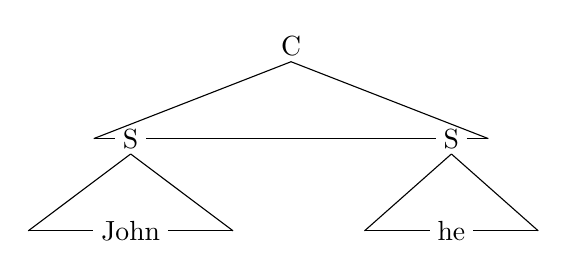
\begin{tikzpicture}
\node at (0.000000, 0.000000) {C};
\node at (-2.036768, -1.171530) {S};
\node at (-2.036768, -2.343060) {John};
\node at (2.036768, -1.171530) {S};
\node at (2.036768, -2.343060) {he};
\draw (0.000000,-0.195255) -- (-2.505383,-1.171530);
\draw (0.000000,-0.195255) -- (2.505383,-1.171530);
\draw (-2.505383,-1.171530) -- (-2.234396,-1.171530);
\draw (-1.839140,-1.171530) -- (1.839140,-1.171530);
\draw (2.234396,-1.171530) -- (2.505383,-1.171530);
\draw (-2.036768,-1.366785) -- (-3.337663,-2.343060);
\draw (-2.036768,-1.366785) -- (-0.735872,-2.343060);
\draw (-3.337663,-2.343060) -- (-2.510195,-2.343060);
\draw (-1.563340,-2.343060) -- (-0.735872,-2.343060);
\draw (2.036768,-1.366785) -- (0.933570,-2.343060);
\draw (2.036768,-1.366785) -- (3.139966,-2.343060);
\draw (0.933570,-2.343060) -- (1.761037,-2.343060);
\draw (2.312498,-2.343060) -- (3.139966,-2.343060);
\end{tikzpicture}
}
\end{minipage}
\bigbreak

\bigbreak
\begin{minipage}{\textwidth}
  \makebox[\textwidth][c]{
  \begin{tabular}{|r|c|c|c|c|c|c|c|c|c|}
    \hline
    \multicolumn{10}{|c|}{\textbf{Features}} \\
    \hline
    & \textbf{\texttt{PNF}}
    & \textbf{\texttt{FPF}} & \textbf{\texttt{SPF}}
    & \textbf{\texttt{TPF}} & \textbf{\texttt{PLF}}
    & \textbf{\texttt{GNF}} & \textbf{\texttt{ANF}}
    & \textbf{\texttt{RPF}} & \textbf{\texttt{GEN}} \\
    \textbf{\texttt{John}} & \texttt{-}
    & \texttt{-} & \texttt{-}
    & \texttt{+} & \texttt{-}
    & \texttt{-} & \texttt{+}
    & \texttt{-} & \texttt{-} \\
    \textbf{\texttt{he}} & \texttt{+}
    & \texttt{-} & \texttt{-}
    & \texttt{+} & \texttt{-}
    & \texttt{-} & \texttt{+}
    & \texttt{-} & \texttt{-} \\
    \hline
  \end{tabular}
  }
\end{minipage}
\bigbreak

\bigbreak
\begin{minipage}{\textwidth}
  \makebox[\textwidth][c]{
  \begin{tabular}{|r|l|}
    \hline
    \multicolumn{2}{|c|}{\textbf{Nodes}} \\
    \hline
    ${\textbf{\textrm{1}}_{\phantom{z}}}$ & \texttt{\texttt{(C,~up:0,~dn:2,~lt:0,~rt:0,~th:2,~nu:1)}} \\
    ${\textbf{\textrm{2}}_{\phantom{z}}}$ & \texttt{\texttt{(S,~up:1,~dn:3,~lt:0,~rt:4,~th:3,~nu:2)}} \\
    ${\textbf{\textrm{3}}_{\phantom{z}}}$ & \texttt{\texttt{(N,~lit:John,~ftr:[---+--+--],~up:2,~dn:0,}} \\
    & \texttt{\texttt{~lt:0,~rt:0,~th:4,~np:3,~ch:0,~co:${\textrm{3}_{\textrm{a}}}$,~ec:${\textrm{3}_{\textrm{b}}}$,}} \\
    & \texttt{\texttt{~pr:0,~su:5,~nu:3)}} \\
    ${\textbf{\textrm{3}}_{\textbf{\textrm{a}}}}$ & \texttt{\texttt{(E,~sub:A,~ftr:[---+--+--],~np:3,~ch:0,~co:${\textrm{3}_{\textrm{b}}}$)}} \\
    ${\textbf{\textrm{3}}_{\textbf{\textrm{b}}}}$ & \texttt{\texttt{(E,~sub:B,~ftr:[---+--+--],~np:3,~ch:${\textrm{5}_{\textrm{a}}}$,~co:0)}} \\
    ${\textbf{\textrm{4}}_{\phantom{z}}}$ & \texttt{\texttt{(S,~up:1,~dn:5,~lt:2,~rt:0,~th:5,~nu:4)}} \\
    ${\textbf{\textrm{5}}_{\phantom{z}}}$ & \texttt{\texttt{(N,~lit:he,~ftr:[+--+--+--],~up:4,~dn:0,}} \\
    & \texttt{\texttt{~lt:0,~rt:0,~th:0,~np:5,~ch:0,~co:${\textrm{5}_{\textrm{a}}}$,~ec:${\textrm{5}_{\textrm{a}}}$,}} \\
    & \texttt{\texttt{~pr:3,~su:0,~nu:5)}} \\
    ${\textbf{\textrm{5}}_{\textbf{\textrm{a}}}}$ & \texttt{\texttt{(E,~sub:A,~ftr:[+--+--+--],~np:5,~ch:0,~co:0)}} \\
    \hline
  \end{tabular}
  }
\end{minipage}
\bigbreak

\bigbreak
\begin{minipage}{\textwidth}
\makebox[\textwidth][c]{
\begin{tikzpicture}[
    every node/.style={align=center},
    dotted line/.style={draw, dotted, thick},
    curved arrow/.style={draw, thick, -{Latex[bend]}},
    ]
\node (S) at (1.214084,0.000000) {S};
\node (John) at (0.505225,-1.171530) {John};
\node (he) at (2.120639,-1.171530) {he};
\draw[dotted line] (S) -- (John);
\draw[dotted line] (S) -- (he);
\draw[dotted line] (John) -- (he);
\node (JohnA) at (0.505225,-2.343060) {${\textrm{John}_{\textrm{a}}}$};
\node (heA) at (2.120639,-2.343060) {${\textrm{he}_{\textrm{a}}}$};
\draw[dotted line] (John) -- (JohnA);
\draw[dotted line] (he) -- (heA);
\node (JohnB) at (0.505225,-3.514590) {${\textrm{John}_{\textrm{b}}}$};
\draw[dotted line] (JohnA) -- (JohnB);
\draw[curved arrow] (JohnB.north east) to [out=58.59,in=-121.41] (heA.south west);
\end{tikzpicture}
}
\end{minipage}
\bigbreak

\bigbreak
\begin{minipage}{\textwidth}
  \makebox[\textwidth][c]{
  \begin{tabular}{|l|l|}
    \hline
    \multicolumn{2}{|c|}{\textbf{Chaining}} \\
    \hline
    \textbf{\texttt{John}} & \textbf{\texttt{he}} \\
    ${\texttt{John}_{\texttt{a}}}$ & ${\texttt{he}_{\texttt{a}}}$ \\
    ${\texttt{John}_{\texttt{b}}}$\texttt{\symbol{94}}${\texttt{he}_{\texttt{a}}}$ &  \\
    \hline
  \end{tabular}
  }
\end{minipage}
\bigbreak

\bigbreak
\begin{minipage}{\textwidth}
  \makebox[\textwidth][c]{
  \begin{tabular}{|c|}
    \hline
    \multicolumn{1}{|c|}{\textbf{Interpretations}} \\
    \hline
    ${\texttt{John}_{\texttt{b}}}$\texttt{\symbol{94}}${\texttt{he}_{\texttt{a}}}$ \\
    \hline
  \end{tabular}
  }
\end{minipage}
\bigbreak

\clearpage

%%%%%%%%%%%%%%%%%%%%%%%%%%%%%%%%%%%%%%%%%%%%%%%%%%%%%%%%%%%%%%%%
%
%     (1.14) He will do it if John can.
%
%%%%%%%%%%%%%%%%%%%%%%%%%%%%%%%%%%%%%%%%%%%%%%%%%%%%%%%%%%%%%%%%

\section*{(1.14) He will do it if John can.}
\addcontentsline{toc}{section}{(1.14) He will do it if John can.}

\bigbreak
\begin{enumerate*}
\item[(1.14)] He will do it if John can.
\end{enumerate*}
\bigbreak
\bigbreak
\begin{minipage}{\textwidth}
\makebox[\textwidth][c]{
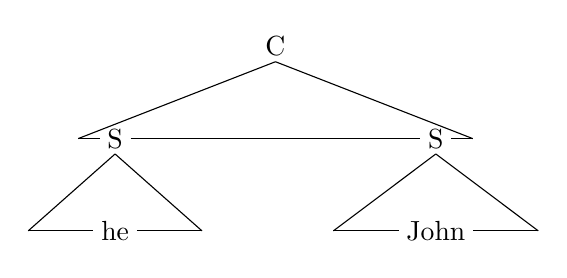
\begin{tikzpicture}
\node at (0.000000, 0.000000) {C};
\node at (-2.036768, -1.171530) {S};
\node at (-2.036768, -2.343060) {he};
\node at (2.036768, -1.171530) {S};
\node at (2.036768, -2.343060) {John};
\draw (0.000000,-0.195255) -- (-2.505383,-1.171530);
\draw (0.000000,-0.195255) -- (2.505383,-1.171530);
\draw (-2.505383,-1.171530) -- (-2.234396,-1.171530);
\draw (-1.839140,-1.171530) -- (1.839140,-1.171530);
\draw (2.234396,-1.171530) -- (2.505383,-1.171530);
\draw (-2.036768,-1.366785) -- (-3.139966,-2.343060);
\draw (-2.036768,-1.366785) -- (-0.933570,-2.343060);
\draw (-3.139966,-2.343060) -- (-2.312498,-2.343060);
\draw (-1.761037,-2.343060) -- (-0.933570,-2.343060);
\draw (2.036768,-1.366785) -- (0.735872,-2.343060);
\draw (2.036768,-1.366785) -- (3.337663,-2.343060);
\draw (0.735872,-2.343060) -- (1.563340,-2.343060);
\draw (2.510195,-2.343060) -- (3.337663,-2.343060);
\end{tikzpicture}
}
\end{minipage}
\bigbreak

\bigbreak
\begin{minipage}{\textwidth}
  \makebox[\textwidth][c]{
  \begin{tabular}{|r|c|c|c|c|c|c|c|c|c|}
    \hline
    \multicolumn{10}{|c|}{\textbf{Features}} \\
    \hline
    & \textbf{\texttt{PNF}}
    & \textbf{\texttt{FPF}} & \textbf{\texttt{SPF}}
    & \textbf{\texttt{TPF}} & \textbf{\texttt{PLF}}
    & \textbf{\texttt{GNF}} & \textbf{\texttt{ANF}}
    & \textbf{\texttt{RPF}} & \textbf{\texttt{GEN}} \\
    \textbf{\texttt{he}} & \texttt{+}
    & \texttt{-} & \texttt{-}
    & \texttt{+} & \texttt{-}
    & \texttt{-} & \texttt{+}
    & \texttt{-} & \texttt{-} \\
    \textbf{\texttt{John}} & \texttt{-}
    & \texttt{-} & \texttt{-}
    & \texttt{+} & \texttt{-}
    & \texttt{-} & \texttt{+}
    & \texttt{-} & \texttt{-} \\
    \hline
  \end{tabular}
  }
\end{minipage}
\bigbreak

\bigbreak
\begin{minipage}{\textwidth}
  \makebox[\textwidth][c]{
  \begin{tabular}{|r|l|}
    \hline
    \multicolumn{2}{|c|}{\textbf{Nodes}} \\
    \hline
    ${\textbf{\textrm{1}}_{\phantom{z}}}$ & \texttt{\texttt{(C,~up:0,~dn:2,~lt:0,~rt:0,~th:2,~nu:1)}} \\
    ${\textbf{\textrm{2}}_{\phantom{z}}}$ & \texttt{\texttt{(S,~up:1,~dn:3,~lt:0,~rt:4,~th:3,~nu:2)}} \\
    ${\textbf{\textrm{3}}_{\phantom{z}}}$ & \texttt{\texttt{(N,~lit:he,~ftr:[+--+--+--],~up:2,~dn:0,}} \\
    & \texttt{\texttt{~lt:0,~rt:0,~th:4,~np:3,~ch:0,~co:${\textrm{3}_{\textrm{a}}}$,~ec:${\textrm{3}_{\textrm{a}}}$,}} \\
    & \texttt{\texttt{~pr:0,~su:5,~nu:3)}} \\
    ${\textbf{\textrm{3}}_{\textbf{\textrm{a}}}}$ & \texttt{\texttt{(E,~sub:A,~ftr:[+--+--+--],~np:3,~ch:0,~co:0)}} \\
    ${\textbf{\textrm{4}}_{\phantom{z}}}$ & \texttt{\texttt{(S,~up:1,~dn:5,~lt:2,~rt:0,~th:5,~nu:4)}} \\
    ${\textbf{\textrm{5}}_{\phantom{z}}}$ & \texttt{\texttt{(N,~lit:John,~ftr:[---+--+--],~up:4,~dn:0,}} \\
    & \texttt{\texttt{~lt:0,~rt:0,~th:0,~np:5,~ch:0,~co:${\textrm{5}_{\textrm{a}}}$,~ec:${\textrm{5}_{\textrm{a}}}$,}} \\
    & \texttt{\texttt{~pr:3,~su:0,~nu:5)}} \\
    ${\textbf{\textrm{5}}_{\textbf{\textrm{a}}}}$ & \texttt{\texttt{(E,~sub:A,~ftr:[---+--+--],~np:5,~ch:0,~co:0)}} \\
    \hline
  \end{tabular}
  }
\end{minipage}
\bigbreak

\bigbreak
\begin{minipage}{\textwidth}
\makebox[\textwidth][c]{
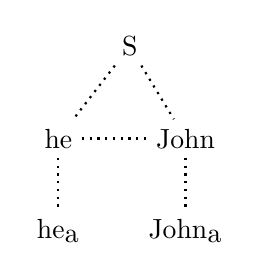
\begin{tikzpicture}[
    every node/.style={align=center},
    dotted line/.style={draw, dotted, thick},
    curved arrow/.style={draw, thick, -{Latex[bend]}},
    ]
\node (S) at (1.214084,0.000000) {S};
\node (he) at (0.307528,-1.171530) {he};
\node (John) at (1.922942,-1.171530) {John};
\draw[dotted line] (S) -- (he);
\draw[dotted line] (S) -- (John);
\draw[dotted line] (he) -- (John);
\node (heA) at (0.307528,-2.343060) {${\textrm{he}_{\textrm{a}}}$};
\node (JohnA) at (1.922942,-2.343060) {${\textrm{John}_{\textrm{a}}}$};
\draw[dotted line] (he) -- (heA);
\draw[dotted line] (John) -- (JohnA);
\end{tikzpicture}
}
\end{minipage}
\bigbreak

\bigbreak
\begin{minipage}{\textwidth}
  \makebox[\textwidth][c]{
  \begin{tabular}{|l|l|}
    \hline
    \multicolumn{2}{|c|}{\textbf{Chaining}} \\
    \hline
    \textbf{\texttt{he}} & \textbf{\texttt{John}} \\
    ${\texttt{he}_{\texttt{a}}}$ & ${\texttt{John}_{\texttt{a}}}$ \\
    \hline
  \end{tabular}
  }
\end{minipage}
\bigbreak

\bigbreak
\begin{minipage}{\textwidth}
  \makebox[\textwidth][c]{
  \begin{tabular}{|c|}
    \hline
    \multicolumn{1}{|c|}{\textbf{Interpretations}} \\
    \hline
    NONE \\
    \hline
  \end{tabular}
  }
\end{minipage}
\bigbreak

\clearpage

%%%%%%%%%%%%%%%%%%%%%%%%%%%%%%%%%%%%%%%%%%%%%%%%%%%%%%%%%%%%%%%%
%
%     (1.24) I have a cat at home, but hate it.
%
%%%%%%%%%%%%%%%%%%%%%%%%%%%%%%%%%%%%%%%%%%%%%%%%%%%%%%%%%%%%%%%%

\section*{(1.24) I have a cat at home, but hate it.}
\addcontentsline{toc}{section}{(1.24) I have a cat at home, but hate it.}

\bigbreak
\begin{enumerate*}
\item[(1.24)] I have a cat at home, but hate it.
\end{enumerate*}
\bigbreak
\bigbreak
\begin{minipage}{\textwidth}
\makebox[\textwidth][c]{
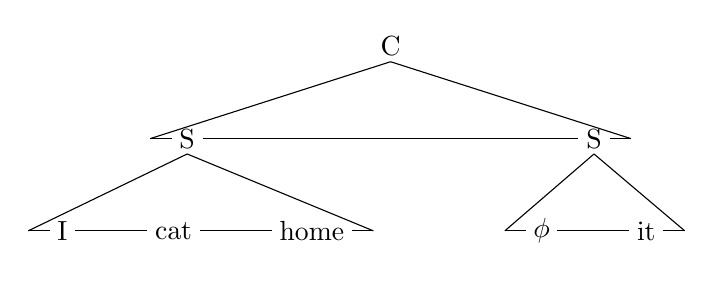
\begin{tikzpicture}
\node at (0.000000, 0.000000) {C};
\node at (-2.583485, -1.171530) {S};
\node at (-4.167501, -2.343060) {I};
\node at (-2.756775, -2.343060) {cat};
\node at (-0.999469, -2.343060) {home};
\node at (2.583485, -1.171530) {S};
\node at (1.919613, -2.343060) {$\phi$};
\node at (3.247356, -2.343060) {it};
\draw (0.000000,-0.195255) -- (-3.052100,-1.171530);
\draw (0.000000,-0.195255) -- (3.052100,-1.171530);
\draw (-3.052100,-1.171530) -- (-2.781113,-1.171530);
\draw (-2.385857,-1.171530) -- (2.385857,-1.171530);
\draw (2.781113,-1.171530) -- (3.052100,-1.171530);
\draw (-2.583485,-1.366785) -- (-4.601946,-2.343060);
\draw (-2.583485,-1.366785) -- (-0.218444,-2.343060);
\draw (-4.601946,-2.343060) -- (-4.330959,-2.343060);
\draw (-4.004043,-2.343060) -- (-3.091082,-2.343060);
\draw (-2.422468,-2.343060) -- (-1.509506,-2.343060);
\draw (-0.489431,-2.343060) -- (-0.218444,-2.343060);
\draw (2.583485,-1.366785) -- (1.450998,-2.343060);
\draw (2.583485,-1.366785) -- (3.735497,-2.343060);
\draw (1.450998,-2.343060) -- (1.721985,-2.343060);
\draw (2.117241,-2.343060) -- (3.030203,-2.343060);
\draw (3.464510,-2.343060) -- (3.735497,-2.343060);
\end{tikzpicture}
}
\end{minipage}
\bigbreak

\bigbreak
\begin{minipage}{\textwidth}
  \makebox[\textwidth][c]{
  \begin{tabular}{|r|c|c|c|c|c|c|c|c|c|}
    \hline
    \multicolumn{10}{|c|}{\textbf{Features}} \\
    \hline
    & \textbf{\texttt{PNF}}
    & \textbf{\texttt{FPF}} & \textbf{\texttt{SPF}}
    & \textbf{\texttt{TPF}} & \textbf{\texttt{PLF}}
    & \textbf{\texttt{GNF}} & \textbf{\texttt{ANF}}
    & \textbf{\texttt{RPF}} & \textbf{\texttt{GEN}} \\
    \textbf{\texttt{I}} & \texttt{+}
    & \texttt{+} & \texttt{-}
    & \texttt{-} & \texttt{-}
    & \texttt{?} & \texttt{+}
    & \texttt{-} & \texttt{-} \\
    \textbf{\texttt{cat}} & \texttt{-}
    & \texttt{-} & \texttt{-}
    & \texttt{+} & \texttt{-}
    & \texttt{?} & \texttt{+}
    & \texttt{-} & \texttt{-} \\
    \textbf{\texttt{home}} & \texttt{-}
    & \texttt{-} & \texttt{-}
    & \texttt{+} & \texttt{-}
    & \texttt{?} & \texttt{-}
    & \texttt{-} & \texttt{-} \\
    $\bm{\phi}$ & \texttt{+}
    & \texttt{?} & \texttt{?}
    & \texttt{?} & \texttt{?}
    & \texttt{?} & \texttt{?}
    & \texttt{-} & \texttt{-} \\
    \textbf{\texttt{it}} & \texttt{+}
    & \texttt{-} & \texttt{-}
    & \texttt{+} & \texttt{-}
    & \texttt{?} & \texttt{-}
    & \texttt{-} & \texttt{-} \\
    \hline
  \end{tabular}
  }
\end{minipage}
\bigbreak

\bigbreak
\begin{minipage}{\textwidth}
  \makebox[\textwidth][c]{
  \begin{tabular}{|r|l|}
    \hline
    \multicolumn{2}{|c|}{\textbf{Nodes}} \\
    \hline
    ${\textbf{\textrm{1}}_{\phantom{z}}}$ & \texttt{\texttt{(C,~up:0,~dn:2,~lt:0,~rt:0,~th:2,~nu:1)}} \\
    ${\textbf{\textrm{2}}_{\phantom{z}}}$ & \texttt{\texttt{(S,~up:1,~dn:3,~lt:0,~rt:6,~th:3,~nu:2)}} \\
    ${\textbf{\textrm{3}}_{\phantom{z}}}$ & \texttt{\texttt{(N,~lit:I,~ftr:[++---?+--],~up:2,~dn:0,}} \\
    & \texttt{\texttt{~lt:0,~rt:4,~th:4,~np:3,~ch:0,~co:${\textrm{3}_{\textrm{a}}}$,~ec:${\textrm{3}_{\textrm{b}}}$,}} \\
    & \texttt{\texttt{~pr:0,~su:4,~nu:3)}} \\
    ${\textbf{\textrm{3}}_{\textbf{\textrm{a}}}}$ & \texttt{\texttt{(E,~sub:A,~ftr:[++---?+--],~np:3,~ch:0,~co:${\textrm{3}_{\textrm{b}}}$)}} \\
    ${\textbf{\textrm{3}}_{\textbf{\textrm{b}}}}$ & \texttt{\texttt{(E,~sub:B,~ftr:[++---?+--],~np:3,~ch:${\textrm{7}_{\textrm{a}}}$,~co:0)}} \\
    ${\textbf{\textrm{4}}_{\phantom{z}}}$ & \texttt{\texttt{(N,~lit:cat,~ftr:[---+-?+--],~up:2,~dn:0,}} \\
    & \texttt{\texttt{~lt:3,~rt:5,~th:5,~np:4,~ch:0,~co:${\textrm{4}_{\textrm{a}}}$,~ec:${\textrm{4}_{\textrm{b}}}$,}} \\
    & \texttt{\texttt{~pr:3,~su:5,~nu:4)}} \\
    ${\textbf{\textrm{4}}_{\textbf{\textrm{a}}}}$ & \texttt{\texttt{(E,~sub:A,~ftr:[---+-?+--],~np:4,~ch:0,~co:${\textrm{4}_{\textrm{b}}}$)}} \\
    ${\textbf{\textrm{4}}_{\textbf{\textrm{b}}}}$ & \texttt{\texttt{(E,~sub:B,~ftr:[---+-?+--],~np:4,~ch:${\textrm{7}_{\textrm{a}}}$,~co:0)}} \\
    ${\textbf{\textrm{5}}_{\phantom{z}}}$ & \texttt{\texttt{(N,~lit:home,~ftr:[---+-?---],~up:2,~dn:0,}} \\
    & \texttt{\texttt{~lt:4,~rt:0,~th:6,~np:5,~ch:0,~co:${\textrm{5}_{\textrm{a}}}$,~ec:${\textrm{5}_{\textrm{c}}}$,}} \\
    & \texttt{\texttt{~pr:4,~su:7,~nu:5)}} \\
    ${\textbf{\textrm{5}}_{\textbf{\textrm{a}}}}$ & \texttt{\texttt{(E,~sub:A,~ftr:[---+-?---],~np:5,~ch:0,~co:${\textrm{5}_{\textrm{b}}}$)}} \\
    ${\textbf{\textrm{5}}_{\textbf{\textrm{b}}}}$ & \texttt{\texttt{(E,~sub:B,~ftr:[---+-?---],~np:5,~ch:${\textrm{8}_{\textrm{a}}}$,~co:${\textrm{5}_{\textrm{c}}}$)}} \\
    ${\textbf{\textrm{5}}_{\textbf{\textrm{c}}}}$ & \texttt{\texttt{(E,~sub:C,~ftr:[---+-?---],~np:5,~ch:${\textrm{7}_{\textrm{a}}}$,~co:0)}} \\
    ${\textbf{\textrm{6}}_{\phantom{z}}}$ & \texttt{\texttt{(S,~up:1,~dn:7,~lt:2,~rt:0,~th:7,~nu:6)}} \\
    ${\textbf{\textrm{7}}_{\phantom{z}}}$ & \texttt{\texttt{(N,~lit:$\phi$,~ftr:[+??????--],~up:6,~dn:0,}} \\
    & \texttt{\texttt{~lt:0,~rt:8,~th:8,~np:7,~ch:0,~co:${\textrm{7}_{\textrm{a}}}$,~ec:${\textrm{7}_{\textrm{a}}}$,}} \\
    & \texttt{\texttt{~pr:5,~su:8,~nu:7)}} \\
    ${\textbf{\textrm{7}}_{\textbf{\textrm{a}}}}$ & \texttt{\texttt{(E,~sub:A,~ftr:[+??????--],~np:7,~ch:0,~co:0)}} \\
    ${\textbf{\textrm{8}}_{\phantom{z}}}$ & \texttt{\texttt{(N,~lit:it,~ftr:[+--+-?---],~up:6,~dn:0,}} \\
    & \texttt{\texttt{~lt:7,~rt:0,~th:0,~np:8,~ch:0,~co:${\textrm{8}_{\textrm{a}}}$,~ec:${\textrm{8}_{\textrm{a}}}$,}} \\
    & \texttt{\texttt{~pr:7,~su:0,~nu:8)}} \\
    ${\textbf{\textrm{8}}_{\textbf{\textrm{a}}}}$ & \texttt{\texttt{(E,~sub:A,~ftr:[+--+-?---],~np:8,~ch:0,~co:0)}} \\
    \hline
  \end{tabular}
  }
\end{minipage}
\bigbreak

\bigbreak
\begin{minipage}{\textwidth}
\makebox[\textwidth][c]{
\begin{tikzpicture}[
    every node/.style={align=center},
    dotted line/.style={draw, dotted, thick},
    curved arrow/.style={draw, thick, -{Latex[bend]}},
    ]
\node (S) at (3.404118,0.000000) {S};
\node (I) at (0.195256,-1.171530) {I};
\node (cat) at (1.559278,-1.171530) {cat};
\node (home) at (3.269879,-1.171530) {home};
\node (PHI) at (5.061024,-1.171530) {$\phi$};
\node (it) at (6.559284,-1.171530) {it};
\draw[dotted line] (S) -- (I);
\draw[dotted line] (S) -- (it);
\draw[dotted line] (I) -- (cat);
\draw[dotted line] (cat) -- (home);
\draw[dotted line] (home) -- (PHI);
\draw[dotted line] (PHI) -- (it);
\node (IA) at (0.195256,-2.343060) {${\textrm{I}_{\textrm{a}}}$};
\node (catA) at (1.559278,-2.343060) {${\textrm{cat}_{\textrm{a}}}$};
\node (homeA) at (3.269879,-2.343060) {${\textrm{home}_{\textrm{a}}}$};
\node (PHIA) at (5.061024,-2.343060) {${\phi_{\textrm{a}}}$};
\node (itA) at (6.559284,-2.343060) {${\textrm{it}_{\textrm{a}}}$};
\draw[dotted line] (I) -- (IA);
\draw[dotted line] (cat) -- (catA);
\draw[dotted line] (home) -- (homeA);
\draw[dotted line] (PHI) -- (PHIA);
\draw[dotted line] (it) -- (itA);
\node (IB) at (0.195256,-3.514590) {${\textrm{I}_{\textrm{b}}}$};
\node (catB) at (1.559278,-3.514590) {${\textrm{cat}_{\textrm{b}}}$};
\node (homeB) at (3.269879,-3.514590) {${\textrm{home}_{\textrm{b}}}$};
\draw[dotted line] (IA) -- (IB);
\draw[dotted line] (catA) -- (catB);
\draw[dotted line] (homeA) -- (homeB);
\node (homeC) at (3.269879,-4.686120) {${\textrm{home}_{\textrm{c}}}$};
\draw[dotted line] (homeB) -- (homeC);
\draw[curved arrow] (homeC.north) to [out=73.02,in=-73.41] (PHIA.south);
\draw[curved arrow] (catB.north east) to [out=39.31,in=-150.27] (PHIA.south west);
\draw[curved arrow] (IB.north east) to [out=28.62,in=144.39] (PHIA.north west);
\draw[curved arrow] (homeB.north east) to [out=39.31,in=-140.69] (itA.south west);
\end{tikzpicture}
}
\end{minipage}
\bigbreak

\bigbreak
\begin{minipage}{\textwidth}
  \makebox[\textwidth][c]{
  \begin{tabular}{|l|l|l|l|l|}
    \hline
    \multicolumn{5}{|c|}{\textbf{Chaining}} \\
    \hline
    \textbf{\texttt{I}} & \textbf{\texttt{cat}}
    & \textbf{\texttt{home}} & $\bm{\phi}$
    & \textbf{\texttt{it}} \\
    ${\texttt{I}_{\texttt{a}}}$ & ${\texttt{cat}_{\texttt{a}}}$
    & ${\texttt{home}_{\texttt{a}}}$ & ${\phi_{\texttt{a}}}$
    & ${\texttt{it}_{\texttt{a}}}$ \\
    ${\texttt{I}_{\texttt{b}}}$\texttt{\symbol{94}}${\phi_{\texttt{a}}}$ & ${\texttt{cat}_{\texttt{b}}}$\texttt{\symbol{94}}${\phi_{\texttt{a}}}$
    & ${\texttt{home}_{\texttt{b}}}$\texttt{\symbol{94}}${\texttt{it}_{\texttt{a}}}$ & 
    &  \\
     & 
    & ${\texttt{home}_{\texttt{c}}}$\texttt{\symbol{94}}${\phi_{\texttt{a}}}$ & 
    &  \\
    \hline
  \end{tabular}
  }
\end{minipage}
\bigbreak

\bigbreak
\begin{minipage}{\textwidth}
  \makebox[\textwidth][c]{
  \begin{tabular}{|c|}
    \hline
    \multicolumn{1}{|c|}{\textbf{Interpretations}} \\
    \hline
    ${\texttt{cat}_{\texttt{b}}}$\texttt{\symbol{94}}${\phi_{\texttt{a}}}$\qquad ${\texttt{home}_{\texttt{b}}}$\texttt{\symbol{94}}${\texttt{it}_{\texttt{a}}}$ \\
    \hline
    ${\texttt{I}_{\texttt{b}}}$\texttt{\symbol{94}}${\phi_{\texttt{a}}}$\qquad ${\texttt{home}_{\texttt{b}}}$\texttt{\symbol{94}}${\texttt{it}_{\texttt{a}}}$ \\
    \hline
  \end{tabular}
  }
\end{minipage}
\bigbreak

\clearpage

%%%%%%%%%%%%%%%%%%%%%%%%%%%%%%%%%%%%%%%%%%%%%%%%%%%%%%%%%%%%%%%%
%
%     (1.25) I want to get a cat for myself.
%
%%%%%%%%%%%%%%%%%%%%%%%%%%%%%%%%%%%%%%%%%%%%%%%%%%%%%%%%%%%%%%%%

\section*{(1.25) I want to get a cat for myself.}
\addcontentsline{toc}{section}{(1.25) I want to get a cat for myself.}

\bigbreak
\begin{enumerate*}
\item[(1.25)] I want to get a cat for myself.
\end{enumerate*}
\bigbreak
\bigbreak
\begin{minipage}{\textwidth}
\makebox[\textwidth][c]{
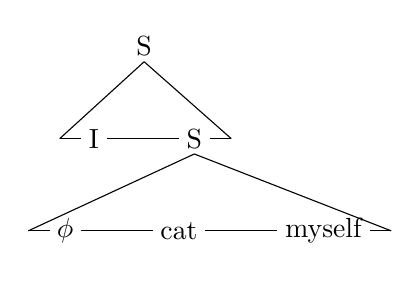
\begin{tikzpicture}
\node at (0.000000, 0.000000) {S};
\node at (-0.637024, -1.171530) {I};
\node at (0.637024, -1.171530) {S};
\node at (-1.003617, -2.343060) {$\phi$};
\node at (0.441280, -2.343060) {cat};
\node at (2.277664, -2.343060) {myself};
\draw (0.000000,-0.195255) -- (-1.071469,-1.171530);
\draw (0.000000,-0.195255) -- (1.105639,-1.171530);
\draw (-1.071469,-1.171530) -- (-0.800482,-1.171530);
\draw (-0.473566,-1.171530) -- (0.439396,-1.171530);
\draw (0.834652,-1.171530) -- (1.105639,-1.171530);
\draw (0.637024,-1.366785) -- (-1.472232,-2.343060);
\draw (0.637024,-1.366785) -- (3.137768,-2.343060);
\draw (-1.472232,-2.343060) -- (-1.201245,-2.343060);
\draw (-0.805989,-2.343060) -- (0.106972,-2.343060);
\draw (0.775587,-2.343060) -- (1.688548,-2.343060);
\draw (2.866781,-2.343060) -- (3.137768,-2.343060);
\end{tikzpicture}
}
\end{minipage}
\bigbreak

\bigbreak
\begin{minipage}{\textwidth}
  \makebox[\textwidth][c]{
  \begin{tabular}{|r|c|c|c|c|c|c|c|c|c|}
    \hline
    \multicolumn{10}{|c|}{\textbf{Features}} \\
    \hline
    & \textbf{\texttt{PNF}}
    & \textbf{\texttt{FPF}} & \textbf{\texttt{SPF}}
    & \textbf{\texttt{TPF}} & \textbf{\texttt{PLF}}
    & \textbf{\texttt{GNF}} & \textbf{\texttt{ANF}}
    & \textbf{\texttt{RPF}} & \textbf{\texttt{GEN}} \\
    \textbf{\texttt{I}} & \texttt{+}
    & \texttt{+} & \texttt{-}
    & \texttt{-} & \texttt{-}
    & \texttt{?} & \texttt{+}
    & \texttt{-} & \texttt{-} \\
    $\bm{\phi}$ & \texttt{+}
    & \texttt{?} & \texttt{?}
    & \texttt{?} & \texttt{?}
    & \texttt{?} & \texttt{?}
    & \texttt{-} & \texttt{-} \\
    \textbf{\texttt{cat}} & \texttt{-}
    & \texttt{-} & \texttt{-}
    & \texttt{+} & \texttt{-}
    & \texttt{?} & \texttt{+}
    & \texttt{-} & \texttt{-} \\
    \textbf{\texttt{myself}} & \texttt{+}
    & \texttt{+} & \texttt{-}
    & \texttt{-} & \texttt{-}
    & \texttt{?} & \texttt{+}
    & \texttt{+} & \texttt{-} \\
    \hline
  \end{tabular}
  }
\end{minipage}
\bigbreak

\bigbreak
\begin{minipage}{\textwidth}
  \makebox[\textwidth][c]{
  \begin{tabular}{|r|l|}
    \hline
    \multicolumn{2}{|c|}{\textbf{Nodes}} \\
    \hline
    ${\textbf{\textrm{1}}_{\phantom{z}}}$ & \texttt{\texttt{(S,~up:0,~dn:2,~lt:0,~rt:0,~th:2,~nu:1)}} \\
    ${\textbf{\textrm{2}}_{\phantom{z}}}$ & \texttt{\texttt{(N,~lit:I,~ftr:[++---?+--],~up:1,~dn:0,}} \\
    & \texttt{\texttt{~lt:0,~rt:3,~th:3,~np:2,~ch:0,~co:${\textrm{2}_{\textrm{a}}}$,~ec:${\textrm{2}_{\textrm{c}}}$,}} \\
    & \texttt{\texttt{~pr:0,~su:4,~nu:2)}} \\
    ${\textbf{\textrm{2}}_{\textbf{\textrm{a}}}}$ & \texttt{\texttt{(E,~sub:A,~ftr:[++---?+--],~np:2,~ch:0,~co:${\textrm{2}_{\textrm{b}}}$)}} \\
    ${\textbf{\textrm{2}}_{\textbf{\textrm{b}}}}$ & \texttt{\texttt{(E,~sub:B,~ftr:[++---?+--],~np:2,~ch:${\textrm{4}_{\textrm{a}}}$,~co:${\textrm{2}_{\textrm{c}}}$)}} \\
    ${\textbf{\textrm{2}}_{\textbf{\textrm{c}}}}$ & \texttt{\texttt{(E,~sub:C,~ftr:[++---?+--],~np:2,~ch:${\textrm{4}_{\textrm{b}}}$,~co:0)}} \\
    ${\textbf{\textrm{3}}_{\phantom{z}}}$ & \texttt{\texttt{(S,~up:1,~dn:4,~lt:2,~rt:0,~th:4,~nu:3)}} \\
    ${\textbf{\textrm{4}}_{\phantom{z}}}$ & \texttt{\texttt{(N,~lit:$\phi$,~ftr:[+??????--],~up:3,~dn:0,}} \\
    & \texttt{\texttt{~lt:0,~rt:5,~th:5,~np:4,~ch:0,~co:${\textrm{4}_{\textrm{a}}}$,~ec:${\textrm{4}_{\textrm{b}}}$,}} \\
    & \texttt{\texttt{~pr:2,~su:5,~nu:4)}} \\
    ${\textbf{\textrm{4}}_{\textbf{\textrm{a}}}}$ & \texttt{\texttt{(E,~sub:A,~ftr:[+??????--],~np:4,~ch:0,~co:${\textrm{4}_{\textrm{b}}}$)}} \\
    ${\textbf{\textrm{4}}_{\textbf{\textrm{b}}}}$ & \texttt{\texttt{(E,~sub:B,~ftr:[++---?+--],~np:4,~ch:${\textrm{6}_{\textrm{a}}}$,~co:0)}} \\
    ${\textbf{\textrm{5}}_{\phantom{z}}}$ & \texttt{\texttt{(N,~lit:cat,~ftr:[---+-?+--],~up:3,~dn:0,}} \\
    & \texttt{\texttt{~lt:4,~rt:6,~th:6,~np:5,~ch:0,~co:${\textrm{5}_{\textrm{a}}}$,~ec:${\textrm{5}_{\textrm{a}}}$,}} \\
    & \texttt{\texttt{~pr:4,~su:6,~nu:5)}} \\
    ${\textbf{\textrm{5}}_{\textbf{\textrm{a}}}}$ & \texttt{\texttt{(E,~sub:A,~ftr:[---+-?+--],~np:5,~ch:0,~co:0)}} \\
    ${\textbf{\textrm{6}}_{\phantom{z}}}$ & \texttt{\texttt{(N,~lit:myself,~ftr:[++---?++-],~up:3,~dn:0,}} \\
    & \texttt{\texttt{~lt:5,~rt:0,~th:0,~np:6,~ch:0,~co:${\textrm{6}_{\textrm{a}}}$,~ec:${\textrm{6}_{\textrm{a}}}$,}} \\
    & \texttt{\texttt{~pr:5,~su:0,~nu:6)}} \\
    ${\textbf{\textrm{6}}_{\textbf{\textrm{a}}}}$ & \texttt{\texttt{(E,~sub:A,~ftr:[++---?++-],~np:6,~ch:0,~co:0)}} \\
    \hline
  \end{tabular}
  }
\end{minipage}
\bigbreak

\bigbreak
\begin{minipage}{\textwidth}
\makebox[\textwidth][c]{
\begin{tikzpicture}[
    every node/.style={align=center},
    dotted line/.style={draw, dotted, thick},
    curved arrow/.style={draw, thick, -{Latex[bend]}},
    ]
\node (S) at (2.832915,0.000000) {S};
\node (I) at (0.195256,-1.171530) {I};
\node (PHI) at (1.639821,-1.171530) {$\phi$};
\node (cat) at (3.255235,-1.171530) {cat};
\node (myself) at (5.044915,-1.171530) {myself};
\draw[dotted line] (S) -- (I);
\draw[dotted line] (S) -- (myself);
\draw[dotted line] (I) -- (PHI);
\draw[dotted line] (PHI) -- (cat);
\draw[dotted line] (cat) -- (myself);
\node (IA) at (0.195256,-2.343060) {${\textrm{I}_{\textrm{a}}}$};
\node (PHIA) at (1.639821,-2.343060) {${\phi_{\textrm{a}}}$};
\node (catA) at (3.255235,-2.343060) {${\textrm{cat}_{\textrm{a}}}$};
\node (myselfA) at (5.044915,-2.343060) {${\textrm{myself}_{\textrm{a}}}$};
\draw[dotted line] (I) -- (IA);
\draw[dotted line] (PHI) -- (PHIA);
\draw[dotted line] (cat) -- (catA);
\draw[dotted line] (myself) -- (myselfA);
\node (IB) at (0.195256,-3.514590) {${\textrm{I}_{\textrm{b}}}$};
\node (PHIB) at (1.639821,-3.514590) {${\phi_{\textrm{b}}}$};
\draw[dotted line] (IA) -- (IB);
\draw[dotted line] (PHIA) -- (PHIB);
\node (IC) at (0.195256,-4.686120) {${\textrm{I}_{\textrm{c}}}$};
\draw[dotted line] (IB) -- (IC);
\draw[curved arrow] (IB.north east) to [out=58.59,in=-121.41] (PHIA.south west);
\draw[curved arrow] (PHIB.north east) to [out=39.31,in=-140.69] (myselfA.south west);
\draw[curved arrow] (IC.north east) to [out=58.59,in=-121.41] (PHIB.south west);
\end{tikzpicture}
}
\end{minipage}
\bigbreak

\bigbreak
\begin{minipage}{\textwidth}
  \makebox[\textwidth][c]{
  \begin{tabular}{|l|l|l|l|}
    \hline
    \multicolumn{4}{|c|}{\textbf{Chaining}} \\
    \hline
    \textbf{\texttt{I}} & $\bm{\phi}$
    & \textbf{\texttt{cat}} & \textbf{\texttt{myself}} \\
    ${\texttt{I}_{\texttt{a}}}$ & ${\phi_{\texttt{a}}}$
    & ${\texttt{cat}_{\texttt{a}}}$ & ${\texttt{myself}_{\texttt{a}}}$ \\
    ${\texttt{I}_{\texttt{b}}}$\texttt{\symbol{94}}${\phi_{\texttt{a}}}$ & ${\phi_{\texttt{b}}}$\texttt{\symbol{94}}${\texttt{myself}_{\texttt{a}}}$
    &  &  \\
    ${\texttt{I}_{\texttt{c}}}$\texttt{\symbol{94}}${\phi_{\texttt{b}}}$ & 
    &  &  \\
    \hline
  \end{tabular}
  }
\end{minipage}
\bigbreak

\bigbreak
\begin{minipage}{\textwidth}
  \makebox[\textwidth][c]{
  \begin{tabular}{|c|}
    \hline
    \multicolumn{1}{|c|}{\textbf{Interpretations}} \\
    \hline
    ${\texttt{I}_{\texttt{c}}}$\texttt{\symbol{94}}${\phi_{\texttt{b}}}$\texttt{\symbol{94}}${\texttt{myself}_{\texttt{a}}}$ \\
    \hline
  \end{tabular}
  }
\end{minipage}
\bigbreak

\clearpage

%%%%%%%%%%%%%%%%%%%%%%%%%%%%%%%%%%%%%%%%%%%%%%%%%%%%%%%%%%%%%%%%
%
%     (1.27) The men took off their hats.
%
%%%%%%%%%%%%%%%%%%%%%%%%%%%%%%%%%%%%%%%%%%%%%%%%%%%%%%%%%%%%%%%%

\section*{(1.27) The men took off their hats.}
\addcontentsline{toc}{section}{(1.27) The men took off their hats.}

\bigbreak
\begin{enumerate*}
\item[(1.27)] The men took off their hats.
\end{enumerate*}
\bigbreak
\bigbreak
\begin{minipage}{\textwidth}
\makebox[\textwidth][c]{
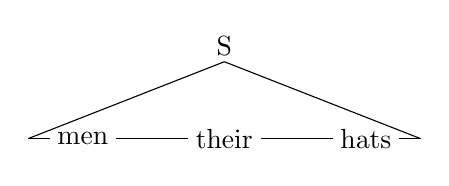
\begin{tikzpicture}
\node at (0.000000, 0.000000) {S};
\node at (-1.797333, -1.171530) {men};
\node at (-0.000488, -1.171530) {their};
\node at (1.797333, -1.171530) {hats};
\draw (0.000000,-0.195255) -- (-2.490493,-1.171530);
\draw (0.000000,-0.195255) -- (2.491469,-1.171530);
\draw (-2.490493,-1.171530) -- (-2.219506,-1.171530);
\draw (-1.375161,-1.171530) -- (-0.462200,-1.171530);
\draw (0.461223,-1.171530) -- (1.374185,-1.171530);
\draw (2.220482,-1.171530) -- (2.491469,-1.171530);
\end{tikzpicture}
}
\end{minipage}
\bigbreak

\bigbreak
\begin{minipage}{\textwidth}
  \makebox[\textwidth][c]{
  \begin{tabular}{|r|c|c|c|c|c|c|c|c|c|}
    \hline
    \multicolumn{10}{|c|}{\textbf{Features}} \\
    \hline
    & \textbf{\texttt{PNF}}
    & \textbf{\texttt{FPF}} & \textbf{\texttt{SPF}}
    & \textbf{\texttt{TPF}} & \textbf{\texttt{PLF}}
    & \textbf{\texttt{GNF}} & \textbf{\texttt{ANF}}
    & \textbf{\texttt{RPF}} & \textbf{\texttt{GEN}} \\
    \textbf{\texttt{men}} & \texttt{-}
    & \texttt{-} & \texttt{-}
    & \texttt{+} & \texttt{+}
    & \texttt{-} & \texttt{+}
    & \texttt{-} & \texttt{-} \\
    \textbf{\texttt{their}} & \texttt{+}
    & \texttt{-} & \texttt{-}
    & \texttt{+} & \texttt{+}
    & \texttt{?} & \texttt{+}
    & \texttt{-} & \texttt{+} \\
    \textbf{\texttt{hats}} & \texttt{-}
    & \texttt{-} & \texttt{-}
    & \texttt{+} & \texttt{+}
    & \texttt{?} & \texttt{-}
    & \texttt{-} & \texttt{-} \\
    \hline
  \end{tabular}
  }
\end{minipage}
\bigbreak

\bigbreak
\begin{minipage}{\textwidth}
  \makebox[\textwidth][c]{
  \begin{tabular}{|r|l|}
    \hline
    \multicolumn{2}{|c|}{\textbf{Nodes}} \\
    \hline
    ${\textbf{\textrm{1}}_{\phantom{z}}}$ & \texttt{\texttt{(S,~up:0,~dn:2,~lt:0,~rt:0,~th:2,~nu:1)}} \\
    ${\textbf{\textrm{2}}_{\phantom{z}}}$ & \texttt{\texttt{(N,~lit:men,~ftr:[---++-+--],~up:1,~dn:0,}} \\
    & \texttt{\texttt{~lt:0,~rt:3,~th:3,~np:2,~ch:0,~co:${\textrm{2}_{\textrm{a}}}$,~ec:${\textrm{2}_{\textrm{b}}}$,}} \\
    & \texttt{\texttt{~pr:0,~su:3,~nu:2)}} \\
    ${\textbf{\textrm{2}}_{\textbf{\textrm{a}}}}$ & \texttt{\texttt{(E,~sub:A,~ftr:[---++-+--],~np:2,~ch:0,~co:${\textrm{2}_{\textrm{b}}}$)}} \\
    ${\textbf{\textrm{2}}_{\textbf{\textrm{b}}}}$ & \texttt{\texttt{(E,~sub:B,~ftr:[---++-+--],~np:2,~ch:${\textrm{3}_{\textrm{a}}}$,~co:0)}} \\
    ${\textbf{\textrm{3}}_{\phantom{z}}}$ & \texttt{\texttt{(N,~lit:their,~ftr:[+--++?+-+],~up:1,~dn:0,}} \\
    & \texttt{\texttt{~lt:2,~rt:4,~th:4,~np:3,~ch:0,~co:${\textrm{3}_{\textrm{a}}}$,~ec:${\textrm{3}_{\textrm{a}}}$,}} \\
    & \texttt{\texttt{~pr:2,~su:4,~nu:3)}} \\
    ${\textbf{\textrm{3}}_{\textbf{\textrm{a}}}}$ & \texttt{\texttt{(E,~sub:A,~ftr:[+--++?+-+],~np:3,~ch:0,~co:0)}} \\
    ${\textbf{\textrm{4}}_{\phantom{z}}}$ & \texttt{\texttt{(N,~lit:hats,~ftr:[---++?---],~up:1,~dn:0,}} \\
    & \texttt{\texttt{~lt:3,~rt:0,~th:0,~np:4,~ch:0,~co:${\textrm{4}_{\textrm{a}}}$,~ec:${\textrm{4}_{\textrm{a}}}$,}} \\
    & \texttt{\texttt{~pr:3,~su:0,~nu:4)}} \\
    ${\textbf{\textrm{4}}_{\textbf{\textrm{a}}}}$ & \texttt{\texttt{(E,~sub:A,~ftr:[---++?---],~np:4,~ch:0,~co:0)}} \\
    \hline
  \end{tabular}
  }
\end{minipage}
\bigbreak

\bigbreak
\begin{minipage}{\textwidth}
\makebox[\textwidth][c]{
\begin{tikzpicture}[
    every node/.style={align=center},
    dotted line/.style={draw, dotted, thick},
    curved arrow/.style={draw, thick, -{Latex[bend]}},
    ]
\node (S) at (2.205087,0.000000) {S};
\node (men) at (0.453970,-1.171530) {men};
\node (their) at (2.204111,-1.171530) {their};
\node (hats) at (3.955228,-1.171530) {hats};
\draw[dotted line] (S) -- (men);
\draw[dotted line] (S) -- (hats);
\draw[dotted line] (men) -- (their);
\draw[dotted line] (their) -- (hats);
\node (menA) at (0.453970,-2.343060) {${\textrm{men}_{\textrm{a}}}$};
\node (theirA) at (2.204111,-2.343060) {${\textrm{their}_{\textrm{a}}}$};
\node (hatsA) at (3.955228,-2.343060) {${\textrm{hats}_{\textrm{a}}}$};
\draw[dotted line] (men) -- (menA);
\draw[dotted line] (their) -- (theirA);
\draw[dotted line] (hats) -- (hatsA);
\node (menB) at (0.453970,-3.514590) {${\textrm{men}_{\textrm{b}}}$};
\draw[dotted line] (menA) -- (menB);
\draw[curved arrow] (menB.north east) to [out=58.59,in=-121.41] (theirA.south west);
\end{tikzpicture}
}
\end{minipage}
\bigbreak

\bigbreak
\begin{minipage}{\textwidth}
  \makebox[\textwidth][c]{
  \begin{tabular}{|l|l|l|}
    \hline
    \multicolumn{3}{|c|}{\textbf{Chaining}} \\
    \hline
    \textbf{\texttt{men}} & \textbf{\texttt{their}}
    & \textbf{\texttt{hats}} \\
    ${\texttt{men}_{\texttt{a}}}$ & ${\texttt{their}_{\texttt{a}}}$
    & ${\texttt{hats}_{\texttt{a}}}$ \\
    ${\texttt{men}_{\texttt{b}}}$\texttt{\symbol{94}}${\texttt{their}_{\texttt{a}}}$ & 
    &  \\
    \hline
  \end{tabular}
  }
\end{minipage}
\bigbreak

\bigbreak
\begin{minipage}{\textwidth}
  \makebox[\textwidth][c]{
  \begin{tabular}{|c|}
    \hline
    \multicolumn{1}{|c|}{\textbf{Interpretations}} \\
    \hline
    ${\texttt{men}_{\texttt{b}}}$\texttt{\symbol{94}}${\texttt{their}_{\texttt{a}}}$ \\
    \hline
  \end{tabular}
  }
\end{minipage}
\bigbreak

\clearpage

%%%%%%%%%%%%%%%%%%%%%%%%%%%%%%%%%%%%%%%%%%%%%%%%%%%%%%%%%%%%%%%%
%
%     (1.51) The man who lives next door said that he would mow my lawn.
%
%%%%%%%%%%%%%%%%%%%%%%%%%%%%%%%%%%%%%%%%%%%%%%%%%%%%%%%%%%%%%%%%

\section*{(1.51) The man who lives next door said that he would mow my lawn.}
\addcontentsline{toc}{section}{(1.51) The man who lives next door said that he would mow my lawn.}

\bigbreak
\begin{enumerate*}
\item[(1.51)] The man who lives next door said that he would mow my lawn.
\end{enumerate*}
\bigbreak
\bigbreak
\begin{minipage}{\textwidth}
\makebox[\textwidth][c]{
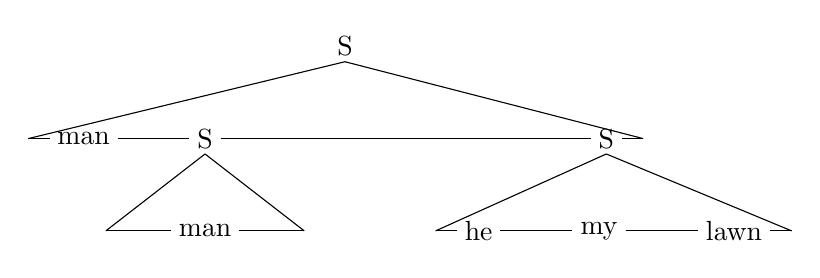
\begin{tikzpicture}
\node at (0.000000, 0.000000) {S};
\node at (-3.319357, -1.171530) {man};
\node at (-1.776832, -1.171530) {S};
\node at (-1.776832, -2.343060) {man};
\node at (3.319357, -1.171530) {S};
\node at (1.698730, -2.343060) {he};
\node at (3.226611, -2.343060) {my};
\node at (4.939985, -2.343060) {lawn};
\draw (0.000000,-0.195255) -- (-4.022280,-1.171530);
\draw (0.000000,-0.195255) -- (3.787973,-1.171530);
\draw (-4.022280,-1.171530) -- (-3.751293,-1.171530);
\draw (-2.887422,-1.171530) -- (-1.974461,-1.171530);
\draw (-1.579204,-1.171530) -- (3.121729,-1.171530);
\draw (3.516985,-1.171530) -- (3.787973,-1.171530);
\draw (-1.776832,-1.366785) -- (-3.036236,-2.343060);
\draw (-1.776832,-1.366785) -- (-0.517429,-2.343060);
\draw (-3.036236,-2.343060) -- (-2.208768,-2.343060);
\draw (-1.344897,-2.343060) -- (-0.517429,-2.343060);
\draw (3.319357,-1.366785) -- (1.152013,-2.343060);
\draw (3.319357,-1.366785) -- (5.672195,-2.343060);
\draw (1.152013,-2.343060) -- (1.423000,-2.343060);
\draw (1.974460,-2.343060) -- (2.887422,-2.343060);
\draw (3.565800,-2.343060) -- (4.478761,-2.343060);
\draw (5.401208,-2.343060) -- (5.672195,-2.343060);
\end{tikzpicture}
}
\end{minipage}
\bigbreak

\bigbreak
\begin{minipage}{\textwidth}
  \makebox[\textwidth][c]{
  \begin{tabular}{|r|c|c|c|c|c|c|c|c|c|}
    \hline
    \multicolumn{10}{|c|}{\textbf{Features}} \\
    \hline
    & \textbf{\texttt{PNF}}
    & \textbf{\texttt{FPF}} & \textbf{\texttt{SPF}}
    & \textbf{\texttt{TPF}} & \textbf{\texttt{PLF}}
    & \textbf{\texttt{GNF}} & \textbf{\texttt{ANF}}
    & \textbf{\texttt{RPF}} & \textbf{\texttt{GEN}} \\
    \textbf{\texttt{man}} & \texttt{-}
    & \texttt{-} & \texttt{-}
    & \texttt{+} & \texttt{-}
    & \texttt{-} & \texttt{+}
    & \texttt{-} & \texttt{-} \\
    \textbf{\texttt{he}} & \texttt{+}
    & \texttt{-} & \texttt{-}
    & \texttt{+} & \texttt{-}
    & \texttt{-} & \texttt{+}
    & \texttt{-} & \texttt{-} \\
    \textbf{\texttt{my}} & \texttt{+}
    & \texttt{+} & \texttt{-}
    & \texttt{-} & \texttt{-}
    & \texttt{?} & \texttt{+}
    & \texttt{-} & \texttt{+} \\
    \textbf{\texttt{lawn}} & \texttt{-}
    & \texttt{-} & \texttt{-}
    & \texttt{+} & \texttt{-}
    & \texttt{?} & \texttt{-}
    & \texttt{-} & \texttt{-} \\
    \hline
  \end{tabular}
  }
\end{minipage}
\bigbreak

\bigbreak
\begin{minipage}{\textwidth}
  \makebox[\textwidth][c]{
  \begin{tabular}{|r|l|}
    \hline
    \multicolumn{2}{|c|}{\textbf{Nodes}} \\
    \hline
    ${\textbf{\textrm{1}}_{\phantom{z}}}$ & \texttt{\texttt{(S,~up:0,~dn:2,~lt:0,~rt:0,~th:2,~nu:1)}} \\
    ${\textbf{\textrm{2}}_{\phantom{z}}}$ & \texttt{\texttt{(N,~lit:man,~ftr:[---+--+--],~up:1,~dn:0,}} \\
    & \texttt{\texttt{~lt:0,~rt:3,~th:3,~np:2,~ch:0,~co:${\textrm{2}_{\textrm{a}}}$,~ec:${\textrm{2}_{\textrm{b}}}$,}} \\
    & \texttt{\texttt{~pr:0,~su:6,~nu:2)}} \\
    ${\textbf{\textrm{2}}_{\textbf{\textrm{a}}}}$ & \texttt{\texttt{(E,~sub:A,~ftr:[---+--+--],~np:2,~ch:0,~co:${\textrm{2}_{\textrm{b}}}$)}} \\
    ${\textbf{\textrm{2}}_{\textbf{\textrm{b}}}}$ & \texttt{\texttt{(E,~sub:B,~ftr:[---+--+--],~np:2,~ch:${\textrm{6}_{\textrm{a}}}$,~co:0)}} \\
    ${\textbf{\textrm{3}}_{\phantom{z}}}$ & \texttt{\texttt{(S,~up:1,~dn:4,~lt:2,~rt:5,~th:4,~nu:3)}} \\
    ${\textbf{\textrm{4}}_{\phantom{z}}}$ & \texttt{\texttt{(N,~lit:man,~ftr:[---+--+--],~up:3,~dn:0,}} \\
    & \texttt{\texttt{~lt:0,~rt:0,~th:5,~np:4,~ch:0,~co:0,~ec:0,}} \\
    & \texttt{\texttt{~pr:0,~su:0,~nu:4)}} \\
    ${\textbf{\textrm{5}}_{\phantom{z}}}$ & \texttt{\texttt{(S,~up:1,~dn:6,~lt:3,~rt:0,~th:6,~nu:5)}} \\
    ${\textbf{\textrm{6}}_{\phantom{z}}}$ & \texttt{\texttt{(N,~lit:he,~ftr:[+--+--+--],~up:5,~dn:0,}} \\
    & \texttt{\texttt{~lt:0,~rt:7,~th:7,~np:6,~ch:0,~co:${\textrm{6}_{\textrm{a}}}$,~ec:${\textrm{6}_{\textrm{a}}}$,}} \\
    & \texttt{\texttt{~pr:2,~su:7,~nu:6)}} \\
    ${\textbf{\textrm{6}}_{\textbf{\textrm{a}}}}$ & \texttt{\texttt{(E,~sub:A,~ftr:[+--+--+--],~np:6,~ch:0,~co:0)}} \\
    ${\textbf{\textrm{7}}_{\phantom{z}}}$ & \texttt{\texttt{(N,~lit:my,~ftr:[++---?+-+],~up:5,~dn:0,}} \\
    & \texttt{\texttt{~lt:6,~rt:8,~th:8,~np:7,~ch:0,~co:${\textrm{7}_{\textrm{a}}}$,~ec:${\textrm{7}_{\textrm{a}}}$,}} \\
    & \texttt{\texttt{~pr:6,~su:8,~nu:7)}} \\
    ${\textbf{\textrm{7}}_{\textbf{\textrm{a}}}}$ & \texttt{\texttt{(E,~sub:A,~ftr:[++---?+-+],~np:7,~ch:0,~co:0)}} \\
    ${\textbf{\textrm{8}}_{\phantom{z}}}$ & \texttt{\texttt{(N,~lit:lawn,~ftr:[---+-?---],~up:5,~dn:0,}} \\
    & \texttt{\texttt{~lt:7,~rt:0,~th:0,~np:8,~ch:0,~co:${\textrm{8}_{\textrm{a}}}$,~ec:${\textrm{8}_{\textrm{a}}}$,}} \\
    & \texttt{\texttt{~pr:7,~su:0,~nu:8)}} \\
    ${\textbf{\textrm{8}}_{\textbf{\textrm{a}}}}$ & \texttt{\texttt{(E,~sub:A,~ftr:[---+-?---],~np:8,~ch:0,~co:0)}} \\
    \hline
  \end{tabular}
  }
\end{minipage}
\bigbreak

\bigbreak
\begin{minipage}{\textwidth}
\makebox[\textwidth][c]{
\begin{tikzpicture}[
    every node/.style={align=center},
    dotted line/.style={draw, dotted, thick},
    curved arrow/.style={draw, thick, -{Latex[bend]}},
    ]
\node (S) at (2.839261,0.000000) {S};
\node (man) at (0.463733,-1.171530) {man};
\node (he) at (2.037656,-1.171530) {he};
\node (my) at (3.518832,-1.171530) {my};
\node (lawn) at (5.185501,-1.171530) {lawn};
\draw[dotted line] (S) -- (man);
\draw[dotted line] (S) -- (lawn);
\draw[dotted line] (man) -- (he);
\draw[dotted line] (he) -- (my);
\draw[dotted line] (my) -- (lawn);
\node (manA) at (0.463733,-2.343060) {${\textrm{man}_{\textrm{a}}}$};
\node (heA) at (2.037656,-2.343060) {${\textrm{he}_{\textrm{a}}}$};
\node (myA) at (3.518832,-2.343060) {${\textrm{my}_{\textrm{a}}}$};
\node (lawnA) at (5.185501,-2.343060) {${\textrm{lawn}_{\textrm{a}}}$};
\draw[dotted line] (man) -- (manA);
\draw[dotted line] (he) -- (heA);
\draw[dotted line] (my) -- (myA);
\draw[dotted line] (lawn) -- (lawnA);
\node (manB) at (0.463733,-3.514590) {${\textrm{man}_{\textrm{b}}}$};
\draw[dotted line] (manA) -- (manB);
\draw[curved arrow] (manB.north east) to [out=58.59,in=-121.41] (heA.south west);
\end{tikzpicture}
}
\end{minipage}
\bigbreak

\bigbreak
\begin{minipage}{\textwidth}
  \makebox[\textwidth][c]{
  \begin{tabular}{|l|l|l|l|}
    \hline
    \multicolumn{4}{|c|}{\textbf{Chaining}} \\
    \hline
    \textbf{\texttt{man}} & \textbf{\texttt{he}}
    & \textbf{\texttt{my}} & \textbf{\texttt{lawn}} \\
    ${\texttt{man}_{\texttt{a}}}$ & ${\texttt{he}_{\texttt{a}}}$
    & ${\texttt{my}_{\texttt{a}}}$ & ${\texttt{lawn}_{\texttt{a}}}$ \\
    ${\texttt{man}_{\texttt{b}}}$\texttt{\symbol{94}}${\texttt{he}_{\texttt{a}}}$ & 
    &  &  \\
    \hline
  \end{tabular}
  }
\end{minipage}
\bigbreak

\bigbreak
\begin{minipage}{\textwidth}
  \makebox[\textwidth][c]{
  \begin{tabular}{|c|}
    \hline
    \multicolumn{1}{|c|}{\textbf{Interpretations}} \\
    \hline
    ${\texttt{man}_{\texttt{b}}}$\texttt{\symbol{94}}${\texttt{he}_{\texttt{a}}}$ \\
    \hline
  \end{tabular}
  }
\end{minipage}
\bigbreak

\clearpage

%%%%%%%%%%%%%%%%%%%%%%%%%%%%%%%%%%%%%%%%%%%%%%%%%%%%%%%%%%%%%%%%
%
%     (1.52) Somebody seduced Bill's sister, but no one will ever seduce Jack’s and she knows it.
%
%%%%%%%%%%%%%%%%%%%%%%%%%%%%%%%%%%%%%%%%%%%%%%%%%%%%%%%%%%%%%%%%

\section*{(1.52) Somebody seduced Bill's sister, but no one will ever seduce Jack’s and she knows it.}
\addcontentsline{toc}{section}{(1.52) Somebody seduced Bill's sister, but no one will ever seduce Jack’s and she knows it.}

\bigbreak
\begin{enumerate*}
\item[(1.52)] Somebody seduced Bill's sister, but no one will ever seduce Jack’s and she knows it.
\end{enumerate*}
\bigbreak
\bigbreak
\begin{minipage}{\textwidth}
\makebox[\textwidth][c]{
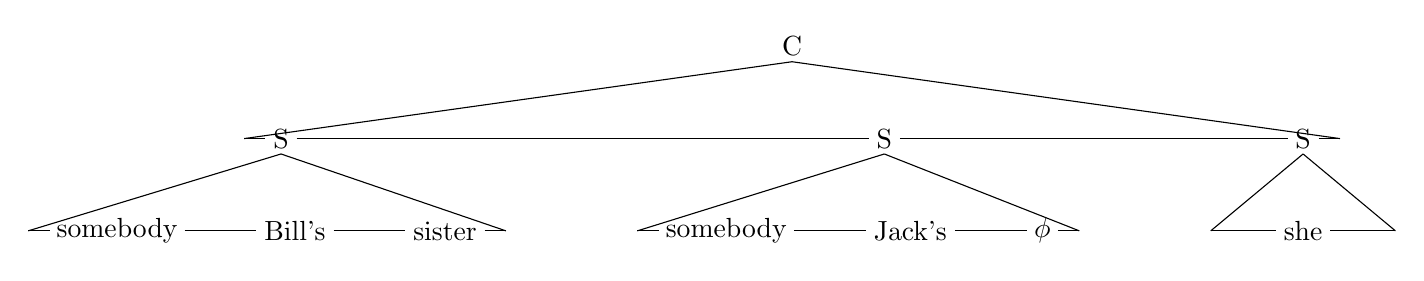
\begin{tikzpicture}
\node at (0.000000, 0.000000) {C};
\node at (-6.489951, -1.171530) {S};
\node at (-8.572115, -2.343060) {somebody};
\node at (-6.312512, -2.343060) {Bill's};
\node at (-4.407788, -2.343060) {sister};
\node at (1.171659, -1.171530) {S};
\node at (-0.836063, -2.343060) {somebody};
\node at (1.501641, -2.343060) {Jack's};
\node at (3.179381, -2.343060) {$\phi$};
\node at (6.489951, -1.171530) {S};
\node at (6.489951, -2.343060) {she};
\draw (0.000000,-0.195255) -- (-6.958567,-1.171530);
\draw (0.000000,-0.195255) -- (6.958567,-1.171530);
\draw (-6.958567,-1.171530) -- (-6.687579,-1.171530);
\draw (-6.292323,-1.171530) -- (0.974031,-1.171530);
\draw (1.369287,-1.171530) -- (6.292323,-1.171530);
\draw (6.687579,-1.171530) -- (6.958567,-1.171530);
\draw (-6.489951,-1.366785) -- (-9.700695,-2.343060);
\draw (-6.489951,-1.366785) -- (-3.634086,-2.343060);
\draw (-9.700695,-2.343060) -- (-9.429708,-2.343060);
\draw (-7.714521,-2.343060) -- (-6.801560,-2.343060);
\draw (-5.823464,-2.343060) -- (-4.910503,-2.343060);
\draw (-3.905073,-2.343060) -- (-3.634086,-2.343060);
\draw (1.171659,-1.366785) -- (-1.964644,-2.343060);
\draw (1.171659,-1.366785) -- (3.647996,-2.343060);
\draw (-1.964644,-2.343060) -- (-1.693657,-2.343060);
\draw (0.021530,-2.343060) -- (0.934491,-2.343060);
\draw (2.068791,-2.343060) -- (2.981753,-2.343060);
\draw (3.377009,-2.343060) -- (3.647996,-2.343060);
\draw (6.489951,-1.366785) -- (5.317438,-2.343060);
\draw (6.489951,-1.366785) -- (7.662465,-2.343060);
\draw (5.317438,-2.343060) -- (6.144906,-2.343060);
\draw (6.834997,-2.343060) -- (7.662465,-2.343060);
\end{tikzpicture}
}
\end{minipage}
\bigbreak

\bigbreak
\begin{minipage}{\textwidth}
  \makebox[\textwidth][c]{
  \begin{tabular}{|r|c|c|c|c|c|c|c|c|c|}
    \hline
    \multicolumn{10}{|c|}{\textbf{Features}} \\
    \hline
    & \textbf{\texttt{PNF}}
    & \textbf{\texttt{FPF}} & \textbf{\texttt{SPF}}
    & \textbf{\texttt{TPF}} & \textbf{\texttt{PLF}}
    & \textbf{\texttt{GNF}} & \textbf{\texttt{ANF}}
    & \textbf{\texttt{RPF}} & \textbf{\texttt{GEN}} \\
    \textbf{\texttt{somebody}} & \texttt{+}
    & \texttt{-} & \texttt{-}
    & \texttt{+} & \texttt{-}
    & \texttt{?} & \texttt{+}
    & \texttt{-} & \texttt{-} \\
    \textbf{\texttt{Bill's}} & \texttt{-}
    & \texttt{-} & \texttt{-}
    & \texttt{+} & \texttt{-}
    & \texttt{-} & \texttt{+}
    & \texttt{-} & \texttt{+} \\
    \textbf{\texttt{sister}} & \texttt{-}
    & \texttt{-} & \texttt{-}
    & \texttt{+} & \texttt{-}
    & \texttt{+} & \texttt{+}
    & \texttt{-} & \texttt{-} \\
    \textbf{\texttt{Jack's}} & \texttt{-}
    & \texttt{-} & \texttt{-}
    & \texttt{+} & \texttt{-}
    & \texttt{-} & \texttt{+}
    & \texttt{-} & \texttt{+} \\
    $\bm{\phi}$ & \texttt{+}
    & \texttt{?} & \texttt{?}
    & \texttt{?} & \texttt{?}
    & \texttt{?} & \texttt{?}
    & \texttt{-} & \texttt{-} \\
    \textbf{\texttt{she}} & \texttt{+}
    & \texttt{-} & \texttt{-}
    & \texttt{+} & \texttt{-}
    & \texttt{+} & \texttt{+}
    & \texttt{-} & \texttt{-} \\
    \hline
  \end{tabular}
  }
\end{minipage}
\bigbreak

\bigbreak
\begin{minipage}{\textwidth}
  \makebox[\textwidth][c]{
  \begin{tabular}{|r|l|}
    \hline
    \multicolumn{2}{|c|}{\textbf{Nodes}} \\
    \hline
    ${\textbf{\textrm{1}}_{\phantom{z}}}$ & \texttt{\texttt{(C,~up:0,~dn:2,~lt:0,~rt:0,~th:2,~nu:1)}} \\
    ${\textbf{\textrm{2}}_{\phantom{z}}}$ & \texttt{\texttt{(S,~up:1,~dn:3,~lt:0,~rt:6,~th:3,~nu:2)}} \\
    ${\textbf{\textrm{3}}_{\phantom{z}}}$ & \texttt{\texttt{(N,~lit:somebody,~ftr:[+--+-?+--],~up:2,~dn:0,}} \\
    & \texttt{\texttt{~lt:0,~rt:4,~th:4,~np:3,~ch:0,~co:${\textrm{3}_{\textrm{a}}}$,~ec:${\textrm{3}_{\textrm{d}}}$,}} \\
    & \texttt{\texttt{~pr:0,~su:4,~nu:3)}} \\
    ${\textbf{\textrm{3}}_{\textbf{\textrm{a}}}}$ & \texttt{\texttt{(E,~sub:A,~ftr:[+--+-?+--],~np:3,~ch:0,~co:${\textrm{3}_{\textrm{b}}}$)}} \\
    ${\textbf{\textrm{3}}_{\textbf{\textrm{b}}}}$ & \texttt{\texttt{(E,~sub:B,~ftr:[+--+-++--],~np:3,~ch:${\textrm{11}_{\textrm{a}}}$,~co:${\textrm{3}_{\textrm{c}}}$)}} \\
    ${\textbf{\textrm{3}}_{\textbf{\textrm{c}}}}$ & \texttt{\texttt{(E,~sub:C,~ftr:[+--+-?+--],~np:3,~ch:${\textrm{9}_{\textrm{a}}}$,~co:${\textrm{3}_{\textrm{d}}}$)}} \\
    ${\textbf{\textrm{3}}_{\textbf{\textrm{d}}}}$ & \texttt{\texttt{(E,~sub:D,~ftr:[+--+-++--],~np:3,~ch:${\textrm{9}_{\textrm{b}}}$,~co:0)}} \\
    ${\textbf{\textrm{4}}_{\phantom{z}}}$ & \texttt{\texttt{(N,~lit:Bill's,~ftr:[---+--+-+],~up:2,~dn:0,}} \\
    & \texttt{\texttt{~lt:3,~rt:5,~th:5,~np:4,~ch:0,~co:${\textrm{4}_{\textrm{a}}}$,~ec:${\textrm{4}_{\textrm{a}}}$,}} \\
    & \texttt{\texttt{~pr:3,~su:5,~nu:4)}} \\
    ${\textbf{\textrm{4}}_{\textbf{\textrm{a}}}}$ & \texttt{\texttt{(E,~sub:A,~ftr:[---+--+-+],~np:4,~ch:0,~co:0)}} \\
    ${\textbf{\textrm{5}}_{\phantom{z}}}$ & \texttt{\texttt{(N,~lit:sister,~ftr:[---+-++--],~up:2,~dn:0,}} \\
    & \texttt{\texttt{~lt:4,~rt:0,~th:6,~np:5,~ch:0,~co:${\textrm{5}_{\textrm{a}}}$,~ec:${\textrm{5}_{\textrm{d}}}$,}} \\
    & \texttt{\texttt{~pr:4,~su:8,~nu:5)}} \\
    ${\textbf{\textrm{5}}_{\textbf{\textrm{a}}}}$ & \texttt{\texttt{(E,~sub:A,~ftr:[---+-++--],~np:5,~ch:0,~co:${\textrm{5}_{\textrm{b}}}$)}} \\
    ${\textbf{\textrm{5}}_{\textbf{\textrm{b}}}}$ & \texttt{\texttt{(E,~sub:B,~ftr:[---+-++--],~np:5,~ch:${\textrm{11}_{\textrm{a}}}$,~co:${\textrm{5}_{\textrm{c}}}$)}} \\
    ${\textbf{\textrm{5}}_{\textbf{\textrm{c}}}}$ & \texttt{\texttt{(E,~sub:C,~ftr:[---+-++--],~np:5,~ch:${\textrm{9}_{\textrm{a}}}$,~co:${\textrm{5}_{\textrm{d}}}$)}} \\
    ${\textbf{\textrm{5}}_{\textbf{\textrm{d}}}}$ & \texttt{\texttt{(E,~sub:D,~ftr:[---+-++--],~np:5,~ch:${\textrm{9}_{\textrm{b}}}$,~co:0)}} \\
    ${\textbf{\textrm{6}}_{\phantom{z}}}$ & \texttt{\texttt{(S,~up:1,~dn:7,~lt:2,~rt:10,~th:7,~nu:6)}} \\
    ${\textbf{\textrm{7}}_{\phantom{z}}}$ & \texttt{\texttt{(N,~lit:somebody,~ftr:[+--+-?+--],~up:6,~dn:0,}} \\
    & \texttt{\texttt{~lt:0,~rt:8,~th:8,~np:7,~ch:0,~co:0,~ec:0,}} \\
    & \texttt{\texttt{~pr:0,~su:0,~nu:7)}} \\
    ${\textbf{\textrm{8}}_{\phantom{z}}}$ & \texttt{\texttt{(N,~lit:Jack's,~ftr:[---+--+-+],~up:6,~dn:0,}} \\
    & \texttt{\texttt{~lt:7,~rt:9,~th:9,~np:8,~ch:0,~co:${\textrm{8}_{\textrm{a}}}$,~ec:${\textrm{8}_{\textrm{a}}}$,}} \\
    & \texttt{\texttt{~pr:5,~su:9,~nu:8)}} \\
    ${\textbf{\textrm{8}}_{\textbf{\textrm{a}}}}$ & \texttt{\texttt{(E,~sub:A,~ftr:[---+--+-+],~np:8,~ch:0,~co:0)}} \\
    ${\textbf{\textrm{9}}_{\phantom{z}}}$ & \texttt{\texttt{(N,~lit:$\phi$,~ftr:[+??????--],~up:6,~dn:0,}} \\
    & \texttt{\texttt{~lt:8,~rt:0,~th:10,~np:9,~ch:0,~co:${\textrm{9}_{\textrm{a}}}$,~ec:${\textrm{9}_{\textrm{b}}}$,}} \\
    & \texttt{\texttt{~pr:8,~su:11,~nu:9)}} \\
    ${\textbf{\textrm{9}}_{\textbf{\textrm{a}}}}$ & \texttt{\texttt{(E,~sub:A,~ftr:[+??????--],~np:9,~ch:0,~co:${\textrm{9}_{\textrm{b}}}$)}} \\
    ${\textbf{\textrm{9}}_{\textbf{\textrm{b}}}}$ & \texttt{\texttt{(E,~sub:B,~ftr:[+--+-++--],~np:9,~ch:${\textrm{11}_{\textrm{a}}}$,~co:0)}} \\
    ${\textbf{\textrm{10}}_{\phantom{z}}}$ & \texttt{\texttt{(S,~up:1,~dn:11,~lt:6,~rt:0,~th:11,~nu:10)}} \\
    ${\textbf{\textrm{11}}_{\phantom{z}}}$ & \texttt{\texttt{(N,~lit:she,~ftr:[+--+-++--],~up:10,~dn:0,}} \\
    & \texttt{\texttt{~lt:0,~rt:0,~th:0,~np:11,~ch:0,~co:${\textrm{11}_{\textrm{a}}}$,~ec:${\textrm{11}_{\textrm{a}}}$,}} \\
    & \texttt{\texttt{~pr:9,~su:0,~nu:11)}} \\
    ${\textbf{\textrm{11}}_{\textbf{\textrm{a}}}}$ & \texttt{\texttt{(E,~sub:A,~ftr:[+--+-++--],~np:11,~ch:0,~co:0)}} \\
    \hline
  \end{tabular}
  }
\end{minipage}
\bigbreak

\bigbreak
\begin{minipage}{\textwidth}
\makebox[\textwidth][c]{
\begin{tikzpicture}[
    every node/.style={align=center},
    dotted line/.style={draw, dotted, thick},
    curved arrow/.style={draw, thick, -{Latex[bend]}},
    ]
\node (S) at (5.373842,0.000000) {S};
\node (somebody) at (0.889391,-1.171530) {somebody};
\node (Bill's) at (3.102289,-1.171530) {Bill's};
\node (sister) at (4.960309,-1.171530) {sister};
\node (Jack's) at (6.896430,-1.171530) {Jack's};
\node (PHI) at (8.744687,-1.171530) {$\phi$};
\node (she) at (10.370840,-1.171530) {she};
\draw[dotted line] (S) -- (somebody);
\draw[dotted line] (S) -- (she);
\draw[dotted line] (somebody) -- (Bill's);
\draw[dotted line] (Bill's) -- (sister);
\draw[dotted line] (sister) -- (Jack's);
\draw[dotted line] (Jack's) -- (PHI);
\draw[dotted line] (PHI) -- (she);
\node (somebodyA) at (0.889391,-2.343060) {${\textrm{somebody}_{\textrm{a}}}$};
\node (Bill'sA) at (3.102289,-2.343060) {${\textrm{Bill's}_{\textrm{a}}}$};
\node (sisterA) at (4.960309,-2.343060) {${\textrm{sister}_{\textrm{a}}}$};
\node (Jack'sA) at (6.896430,-2.343060) {${\textrm{Jack's}_{\textrm{a}}}$};
\node (PHIA) at (8.744687,-2.343060) {${\phi_{\textrm{a}}}$};
\node (sheA) at (10.370840,-2.343060) {${\textrm{she}_{\textrm{a}}}$};
\draw[dotted line] (somebody) -- (somebodyA);
\draw[dotted line] (Bill's) -- (Bill'sA);
\draw[dotted line] (sister) -- (sisterA);
\draw[dotted line] (Jack's) -- (Jack'sA);
\draw[dotted line] (PHI) -- (PHIA);
\draw[dotted line] (she) -- (sheA);
\node (somebodyB) at (0.889391,-3.514590) {${\textrm{somebody}_{\textrm{b}}}$};
\node (sisterB) at (4.960309,-3.514590) {${\textrm{sister}_{\textrm{b}}}$};
\node (PHIB) at (8.744687,-3.514590) {${\phi_{\textrm{b}}}$};
\draw[dotted line] (somebodyA) -- (somebodyB);
\draw[dotted line] (sisterA) -- (sisterB);
\draw[dotted line] (PHIA) -- (PHIB);
\node (somebodyC) at (0.889391,-4.686120) {${\textrm{somebody}_{\textrm{c}}}$};
\node (sisterC) at (4.960309,-4.686120) {${\textrm{sister}_{\textrm{c}}}$};
\draw[dotted line] (somebodyB) -- (somebodyC);
\draw[dotted line] (sisterB) -- (sisterC);
\node (somebodyD) at (0.889391,-5.857650) {${\textrm{somebody}_{\textrm{d}}}$};
\node (sisterD) at (4.960309,-5.857650) {${\textrm{sister}_{\textrm{d}}}$};
\draw[dotted line] (somebodyC) -- (somebodyD);
\draw[dotted line] (sisterC) -- (sisterD);
\draw[curved arrow] (PHIB.north east) to [out=58.59,in=-85.94] (sheA.south);
\draw[curved arrow] (sisterB.north east) to [out=28.62,in=-160.92] (sheA.west);
\draw[curved arrow] (somebodyB.east) to [out=18.13,in=133.83] (sheA.north west);
\draw[curved arrow] (sisterC.north east) to [out=58.59,in=-81.23] (PHIA.south);
\draw[curved arrow] (somebodyC.north east) to [out=39.31,in=179.13] (PHIA.west);
\draw[curved arrow] (sisterD.north east) to [out=58.59,in=-81.23] (PHIB.south);
\draw[curved arrow] (somebodyD.north east) to [out=39.31,in=179.13] (PHIB.west);
\end{tikzpicture}
}
\end{minipage}
\bigbreak

\bigbreak
\begin{minipage}{\textwidth}
  \makebox[\textwidth][c]{
  \begin{tabular}{|l|l|l|l|l|l|}
    \hline
    \multicolumn{6}{|c|}{\textbf{Chaining}} \\
    \hline
    \textbf{\texttt{somebody}} & \textbf{\texttt{Bill's}}
    & \textbf{\texttt{sister}} & \textbf{\texttt{Jack's}}
    & $\bm{\phi}$ & \textbf{\texttt{she}} \\
    ${\texttt{somebody}_{\texttt{a}}}$ & ${\texttt{Bill's}_{\texttt{a}}}$
    & ${\texttt{sister}_{\texttt{a}}}$ & ${\texttt{Jack's}_{\texttt{a}}}$
    & ${\phi_{\texttt{a}}}$ & ${\texttt{she}_{\texttt{a}}}$ \\
    ${\texttt{somebody}_{\texttt{b}}}$\texttt{\symbol{94}}${\texttt{she}_{\texttt{a}}}$ & 
    & ${\texttt{sister}_{\texttt{b}}}$\texttt{\symbol{94}}${\texttt{she}_{\texttt{a}}}$ & 
    & ${\phi_{\texttt{b}}}$\texttt{\symbol{94}}${\texttt{she}_{\texttt{a}}}$ &  \\
    ${\texttt{somebody}_{\texttt{c}}}$\texttt{\symbol{94}}${\phi_{\texttt{a}}}$ & 
    & ${\texttt{sister}_{\texttt{c}}}$\texttt{\symbol{94}}${\phi_{\texttt{a}}}$ & 
    &  &  \\
    ${\texttt{somebody}_{\texttt{d}}}$\texttt{\symbol{94}}${\phi_{\texttt{b}}}$ & 
    & ${\texttt{sister}_{\texttt{d}}}$\texttt{\symbol{94}}${\phi_{\texttt{b}}}$ & 
    &  &  \\
    \hline
  \end{tabular}
  }
\end{minipage}
\bigbreak

\bigbreak
\begin{minipage}{\textwidth}
  \makebox[\textwidth][c]{
  \begin{tabular}{|c|}
    \hline
    \multicolumn{1}{|c|}{\textbf{Interpretations}} \\
    \hline
    NONE \\
    \hline
  \end{tabular}
  }
\end{minipage}
\bigbreak

\clearpage

%%%%%%%%%%%%%%%%%%%%%%%%%%%%%%%%%%%%%%%%%%%%%%%%%%%%%%%%%%%%%%%%
%
%     (1.66) Realizing that he was unpopular didn't disturb Oscar.
%
%%%%%%%%%%%%%%%%%%%%%%%%%%%%%%%%%%%%%%%%%%%%%%%%%%%%%%%%%%%%%%%%

\section*{(1.66) Realizing that he was unpopular didn't disturb Oscar.}
\addcontentsline{toc}{section}{(1.66) Realizing that he was unpopular didn't disturb Oscar.}

\bigbreak
\begin{enumerate*}
\item[(1.66)] Realizing that he was unpopular didn't disturb Oscar.
\end{enumerate*}
\bigbreak
\bigbreak
\begin{minipage}{\textwidth}
\makebox[\textwidth][c]{
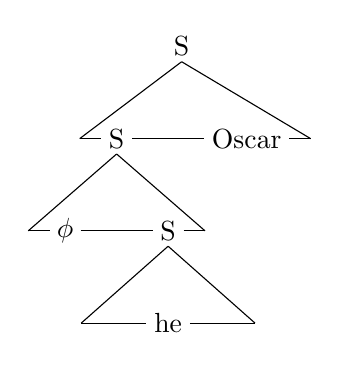
\begin{tikzpicture}
\node at (0.000000, 0.000000) {S};
\node at (-0.825690, -1.171530) {S};
\node at (-1.479798, -2.343060) {$\phi$};
\node at (-0.171581, -2.343060) {S};
\node at (-0.171581, -3.514590) {he};
\node at (0.825690, -1.171530) {Oscar};
\draw (0.000000,-0.195255) -- (-1.294305,-1.171530);
\draw (0.000000,-0.195255) -- (1.637467,-1.171530);
\draw (-1.294305,-1.171530) -- (-1.023318,-1.171530);
\draw (-0.628062,-1.171530) -- (0.284900,-1.171530);
\draw (1.366480,-1.171530) -- (1.637467,-1.171530);
\draw (-0.825690,-1.366785) -- (-1.948414,-2.343060);
\draw (-0.825690,-1.366785) -- (0.297034,-2.343060);
\draw (-1.948414,-2.343060) -- (-1.677426,-2.343060);
\draw (-1.282170,-2.343060) -- (-0.369209,-2.343060);
\draw (0.026047,-2.343060) -- (0.297034,-2.343060);
\draw (-0.171581,-2.538315) -- (-1.274779,-3.514590);
\draw (-0.171581,-2.538315) -- (0.931617,-3.514590);
\draw (-1.274779,-3.514590) -- (-0.447311,-3.514590);
\draw (0.104149,-3.514590) -- (0.931617,-3.514590);
\end{tikzpicture}
}
\end{minipage}
\bigbreak

\bigbreak
\begin{minipage}{\textwidth}
  \makebox[\textwidth][c]{
  \begin{tabular}{|r|c|c|c|c|c|c|c|c|c|}
    \hline
    \multicolumn{10}{|c|}{\textbf{Features}} \\
    \hline
    & \textbf{\texttt{PNF}}
    & \textbf{\texttt{FPF}} & \textbf{\texttt{SPF}}
    & \textbf{\texttt{TPF}} & \textbf{\texttt{PLF}}
    & \textbf{\texttt{GNF}} & \textbf{\texttt{ANF}}
    & \textbf{\texttt{RPF}} & \textbf{\texttt{GEN}} \\
    $\bm{\phi}$ & \texttt{+}
    & \texttt{?} & \texttt{?}
    & \texttt{?} & \texttt{?}
    & \texttt{?} & \texttt{?}
    & \texttt{-} & \texttt{-} \\
    \textbf{\texttt{he}} & \texttt{+}
    & \texttt{-} & \texttt{-}
    & \texttt{+} & \texttt{-}
    & \texttt{-} & \texttt{+}
    & \texttt{-} & \texttt{-} \\
    \textbf{\texttt{Oscar}} & \texttt{-}
    & \texttt{-} & \texttt{-}
    & \texttt{+} & \texttt{-}
    & \texttt{-} & \texttt{+}
    & \texttt{-} & \texttt{-} \\
    \hline
  \end{tabular}
  }
\end{minipage}
\bigbreak

\bigbreak
\begin{minipage}{\textwidth}
  \makebox[\textwidth][c]{
  \begin{tabular}{|r|l|}
    \hline
    \multicolumn{2}{|c|}{\textbf{Nodes}} \\
    \hline
    ${\textbf{\textrm{1}}_{\phantom{z}}}$ & \texttt{\texttt{(S,~up:0,~dn:2,~lt:0,~rt:0,~th:2,~nu:1)}} \\
    ${\textbf{\textrm{2}}_{\phantom{z}}}$ & \texttt{\texttt{(S,~up:1,~dn:3,~lt:0,~rt:6,~th:3,~nu:2)}} \\
    ${\textbf{\textrm{3}}_{\phantom{z}}}$ & \texttt{\texttt{(N,~lit:$\phi$,~ftr:[+??????--],~up:2,~dn:0,}} \\
    & \texttt{\texttt{~lt:0,~rt:4,~th:4,~np:3,~ch:0,~co:${\textrm{3}_{\textrm{a}}}$,~ec:${\textrm{3}_{\textrm{b}}}$,}} \\
    & \texttt{\texttt{~pr:0,~su:5,~nu:3)}} \\
    ${\textbf{\textrm{3}}_{\textbf{\textrm{a}}}}$ & \texttt{\texttt{(E,~sub:A,~ftr:[+??????--],~np:3,~ch:0,~co:${\textrm{3}_{\textrm{b}}}$)}} \\
    ${\textbf{\textrm{3}}_{\textbf{\textrm{b}}}}$ & \texttt{\texttt{(E,~sub:B,~ftr:[+--+--+--],~np:3,~ch:${\textrm{5}_{\textrm{a}}}$,~co:0)}} \\
    ${\textbf{\textrm{4}}_{\phantom{z}}}$ & \texttt{\texttt{(S,~up:2,~dn:5,~lt:3,~rt:0,~th:5,~nu:4)}} \\
    ${\textbf{\textrm{5}}_{\phantom{z}}}$ & \texttt{\texttt{(N,~lit:he,~ftr:[+--+--+--],~up:4,~dn:0,}} \\
    & \texttt{\texttt{~lt:0,~rt:0,~th:6,~np:5,~ch:0,~co:${\textrm{5}_{\textrm{a}}}$,~ec:${\textrm{5}_{\textrm{a}}}$,}} \\
    & \texttt{\texttt{~pr:3,~su:6,~nu:5)}} \\
    ${\textbf{\textrm{5}}_{\textbf{\textrm{a}}}}$ & \texttt{\texttt{(E,~sub:A,~ftr:[+--+--+--],~np:5,~ch:0,~co:0)}} \\
    ${\textbf{\textrm{6}}_{\phantom{z}}}$ & \texttt{\texttt{(N,~lit:Oscar,~ftr:[---+--+--],~up:1,~dn:0,}} \\
    & \texttt{\texttt{~lt:2,~rt:0,~th:0,~np:6,~ch:0,~co:${\textrm{6}_{\textrm{a}}}$,~ec:${\textrm{6}_{\textrm{d}}}$,}} \\
    & \texttt{\texttt{~pr:5,~su:0,~nu:6)}} \\
    ${\textbf{\textrm{6}}_{\textbf{\textrm{a}}}}$ & \texttt{\texttt{(E,~sub:A,~ftr:[---+--+--],~np:6,~ch:0,~co:${\textrm{6}_{\textrm{b}}}$)}} \\
    ${\textbf{\textrm{6}}_{\textbf{\textrm{b}}}}$ & \texttt{\texttt{(E,~sub:B,~ftr:[---+--+--],~np:6,~ch:${\textrm{5}_{\textrm{a}}}$,~co:${\textrm{6}_{\textrm{c}}}$)}} \\
    ${\textbf{\textrm{6}}_{\textbf{\textrm{c}}}}$ & \texttt{\texttt{(E,~sub:C,~ftr:[---+--+--],~np:6,~ch:${\textrm{3}_{\textrm{a}}}$,~co:${\textrm{6}_{\textrm{d}}}$)}} \\
    ${\textbf{\textrm{6}}_{\textbf{\textrm{d}}}}$ & \texttt{\texttt{(E,~sub:D,~ftr:[---+--+--],~np:6,~ch:${\textrm{3}_{\textrm{b}}}$,~co:0)}} \\
    \hline
  \end{tabular}
  }
\end{minipage}
\bigbreak

\bigbreak
\begin{minipage}{\textwidth}
\makebox[\textwidth][c]{
\begin{tikzpicture}[
    every node/.style={align=center},
    dotted line/.style={draw, dotted, thick},
    curved arrow/.style={draw, thick, -{Latex[bend]}},
    ]
\node (S) at (2.129425,0.000000) {S};
\node (PHI) at (0.446648,-1.171530) {$\phi$};
\node (he) at (2.003485,-1.171530) {he};
\node (Oscar) at (3.686262,-1.171530) {Oscar};
\draw[dotted line] (S) -- (PHI);
\draw[dotted line] (S) -- (Oscar);
\draw[dotted line] (PHI) -- (he);
\draw[dotted line] (he) -- (Oscar);
\node (PHIA) at (0.446648,-2.343060) {${\phi_{\textrm{a}}}$};
\node (heA) at (2.003485,-2.343060) {${\textrm{he}_{\textrm{a}}}$};
\node (OscarA) at (3.686262,-2.343060) {${\textrm{Oscar}_{\textrm{a}}}$};
\draw[dotted line] (PHI) -- (PHIA);
\draw[dotted line] (he) -- (heA);
\draw[dotted line] (Oscar) -- (OscarA);
\node (PHIB) at (0.446648,-3.514590) {${\phi_{\textrm{b}}}$};
\node (OscarB) at (3.686262,-3.514590) {${\textrm{Oscar}_{\textrm{b}}}$};
\draw[dotted line] (PHIA) -- (PHIB);
\draw[dotted line] (OscarA) -- (OscarB);
\node (OscarC) at (3.686262,-4.686120) {${\textrm{Oscar}_{\textrm{c}}}$};
\draw[dotted line] (OscarB) -- (OscarC);
\node (OscarD) at (3.686262,-5.857650) {${\textrm{Oscar}_{\textrm{d}}}$};
\draw[dotted line] (OscarC) -- (OscarD);
\draw[curved arrow] (OscarB.north west) to [out=121.41,in=-29.29] (heA.south east);
\draw[curved arrow] (PHIB.north east) to [out=58.59,in=-150.71] (heA.south west);
\draw[curved arrow] (OscarC.north west) to [out=121.41,in=-58.59] (PHIA.south east);
\draw[curved arrow] (OscarD.north west) to [out=121.41,in=-58.59] (PHIB.south east);
\end{tikzpicture}
}
\end{minipage}
\bigbreak

\bigbreak
\begin{minipage}{\textwidth}
  \makebox[\textwidth][c]{
  \begin{tabular}{|l|l|l|}
    \hline
    \multicolumn{3}{|c|}{\textbf{Chaining}} \\
    \hline
    $\bm{\phi}$ & \textbf{\texttt{he}}
    & \textbf{\texttt{Oscar}} \\
    ${\phi_{\texttt{a}}}$ & ${\texttt{he}_{\texttt{a}}}$
    & ${\texttt{Oscar}_{\texttt{a}}}$ \\
    ${\phi_{\texttt{b}}}$\texttt{\symbol{94}}${\texttt{he}_{\texttt{a}}}$ & 
    & ${\texttt{Oscar}_{\texttt{b}}}$\texttt{\symbol{94}}${\texttt{he}_{\texttt{a}}}$ \\
     & 
    & ${\texttt{Oscar}_{\texttt{c}}}$\texttt{\symbol{94}}${\phi_{\texttt{a}}}$ \\
     & 
    & ${\texttt{Oscar}_{\texttt{d}}}$\texttt{\symbol{94}}${\phi_{\texttt{b}}}$ \\
    \hline
  \end{tabular}
  }
\end{minipage}
\bigbreak

\bigbreak
\begin{minipage}{\textwidth}
  \makebox[\textwidth][c]{
  \begin{tabular}{|c|}
    \hline
    \multicolumn{1}{|c|}{\textbf{Interpretations}} \\
    \hline
    ${\texttt{Oscar}_{\texttt{d}}}$\texttt{\symbol{94}}${\phi_{\texttt{b}}}$\texttt{\symbol{94}}${\texttt{he}_{\texttt{a}}}$ \\
    \hline
  \end{tabular}
  }
\end{minipage}
\bigbreak

\clearpage

%%%%%%%%%%%%%%%%%%%%%%%%%%%%%%%%%%%%%%%%%%%%%%%%%%%%%%%%%%%%%%%%
%
%     (1.70) My neighbor who is pregnant said that she was very happy.
%
%%%%%%%%%%%%%%%%%%%%%%%%%%%%%%%%%%%%%%%%%%%%%%%%%%%%%%%%%%%%%%%%

\section*{(1.70) My neighbor who is pregnant said that she was very happy.}
\addcontentsline{toc}{section}{(1.70) My neighbor who is pregnant said that she was very happy.}

\bigbreak
\begin{enumerate*}
\item[(1.70)] My neighbor who is pregnant said that she was very happy.
\end{enumerate*}
\bigbreak
\bigbreak
\begin{minipage}{\textwidth}
\makebox[\textwidth][c]{
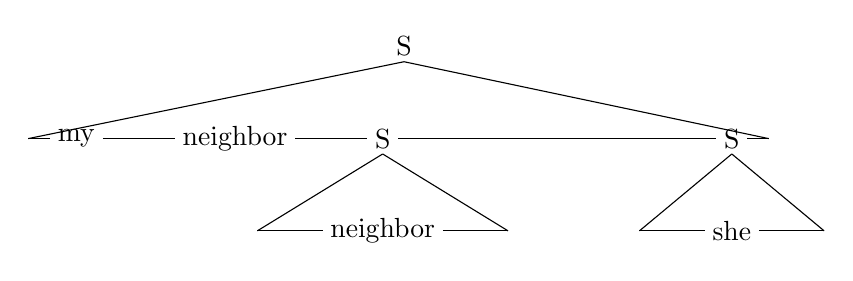
\begin{tikzpicture}
\node at (0.000000, 0.000000) {S};
\node at (-4.162620, -1.171530) {my};
\node at (-2.146111, -1.171530) {neighbor};
\node at (-0.271163, -1.171530) {S};
\node at (-0.271163, -2.343060) {neighbor};
\node at (4.162620, -1.171530) {S};
\node at (4.162620, -2.343060) {she};
\draw (0.000000,-0.195255) -- (-4.772796,-1.171530);
\draw (0.000000,-0.195255) -- (4.631235,-1.171530);
\draw (-4.772796,-1.171530) -- (-4.501808,-1.171530);
\draw (-3.823431,-1.171530) -- (-2.910469,-1.171530);
\draw (-1.381752,-1.171530) -- (-0.468791,-1.171530);
\draw (-0.073535,-1.171530) -- (3.964992,-1.171530);
\draw (4.360248,-1.171530) -- (4.631235,-1.171530);
\draw (-0.271163,-1.366785) -- (-1.862989,-2.343060);
\draw (-0.271163,-1.366785) -- (1.320664,-2.343060);
\draw (-1.862989,-2.343060) -- (-1.035521,-2.343060);
\draw (0.493196,-2.343060) -- (1.320664,-2.343060);
\draw (4.162620,-1.366785) -- (2.990106,-2.343060);
\draw (4.162620,-1.366785) -- (5.335133,-2.343060);
\draw (2.990106,-2.343060) -- (3.817574,-2.343060);
\draw (4.507665,-2.343060) -- (5.335133,-2.343060);
\end{tikzpicture}
}
\end{minipage}
\bigbreak

\bigbreak
\begin{minipage}{\textwidth}
  \makebox[\textwidth][c]{
  \begin{tabular}{|r|c|c|c|c|c|c|c|c|c|}
    \hline
    \multicolumn{10}{|c|}{\textbf{Features}} \\
    \hline
    & \textbf{\texttt{PNF}}
    & \textbf{\texttt{FPF}} & \textbf{\texttt{SPF}}
    & \textbf{\texttt{TPF}} & \textbf{\texttt{PLF}}
    & \textbf{\texttt{GNF}} & \textbf{\texttt{ANF}}
    & \textbf{\texttt{RPF}} & \textbf{\texttt{GEN}} \\
    \textbf{\texttt{my}} & \texttt{+}
    & \texttt{+} & \texttt{-}
    & \texttt{-} & \texttt{-}
    & \texttt{?} & \texttt{+}
    & \texttt{-} & \texttt{+} \\
    \textbf{\texttt{neighbor}} & \texttt{-}
    & \texttt{-} & \texttt{-}
    & \texttt{+} & \texttt{-}
    & \texttt{?} & \texttt{+}
    & \texttt{-} & \texttt{-} \\
    \textbf{\texttt{she}} & \texttt{+}
    & \texttt{-} & \texttt{-}
    & \texttt{+} & \texttt{-}
    & \texttt{+} & \texttt{+}
    & \texttt{-} & \texttt{-} \\
    \hline
  \end{tabular}
  }
\end{minipage}
\bigbreak

\bigbreak
\begin{minipage}{\textwidth}
  \makebox[\textwidth][c]{
  \begin{tabular}{|r|l|}
    \hline
    \multicolumn{2}{|c|}{\textbf{Nodes}} \\
    \hline
    ${\textbf{\textrm{1}}_{\phantom{z}}}$ & \texttt{\texttt{(S,~up:0,~dn:2,~lt:0,~rt:0,~th:2,~nu:1)}} \\
    ${\textbf{\textrm{2}}_{\phantom{z}}}$ & \texttt{\texttt{(N,~lit:my,~ftr:[++---?+-+],~up:1,~dn:0,}} \\
    & \texttt{\texttt{~lt:0,~rt:3,~th:3,~np:2,~ch:0,~co:${\textrm{2}_{\textrm{a}}}$,~ec:${\textrm{2}_{\textrm{a}}}$,}} \\
    & \texttt{\texttt{~pr:0,~su:3,~nu:2)}} \\
    ${\textbf{\textrm{2}}_{\textbf{\textrm{a}}}}$ & \texttt{\texttt{(E,~sub:A,~ftr:[++---?+-+],~np:2,~ch:0,~co:0)}} \\
    ${\textbf{\textrm{3}}_{\phantom{z}}}$ & \texttt{\texttt{(N,~lit:neighbor,~ftr:[---+-?+--],~up:1,~dn:0,}} \\
    & \texttt{\texttt{~lt:2,~rt:4,~th:4,~np:3,~ch:0,~co:${\textrm{3}_{\textrm{a}}}$,~ec:${\textrm{3}_{\textrm{b}}}$,}} \\
    & \texttt{\texttt{~pr:2,~su:7,~nu:3)}} \\
    ${\textbf{\textrm{3}}_{\textbf{\textrm{a}}}}$ & \texttt{\texttt{(E,~sub:A,~ftr:[---+-?+--],~np:3,~ch:0,~co:${\textrm{3}_{\textrm{b}}}$)}} \\
    ${\textbf{\textrm{3}}_{\textbf{\textrm{b}}}}$ & \texttt{\texttt{(E,~sub:B,~ftr:[---+-++--],~np:3,~ch:${\textrm{7}_{\textrm{a}}}$,~co:0)}} \\
    ${\textbf{\textrm{4}}_{\phantom{z}}}$ & \texttt{\texttt{(S,~up:1,~dn:5,~lt:3,~rt:6,~th:5,~nu:4)}} \\
    ${\textbf{\textrm{5}}_{\phantom{z}}}$ & \texttt{\texttt{(N,~lit:neighbor,~ftr:[---+-?+--],~up:4,~dn:0,}} \\
    & \texttt{\texttt{~lt:0,~rt:0,~th:6,~np:5,~ch:0,~co:0,~ec:0,}} \\
    & \texttt{\texttt{~pr:0,~su:0,~nu:5)}} \\
    ${\textbf{\textrm{6}}_{\phantom{z}}}$ & \texttt{\texttt{(S,~up:1,~dn:7,~lt:4,~rt:0,~th:7,~nu:6)}} \\
    ${\textbf{\textrm{7}}_{\phantom{z}}}$ & \texttt{\texttt{(N,~lit:she,~ftr:[+--+-++--],~up:6,~dn:0,}} \\
    & \texttt{\texttt{~lt:0,~rt:0,~th:0,~np:7,~ch:0,~co:${\textrm{7}_{\textrm{a}}}$,~ec:${\textrm{7}_{\textrm{a}}}$,}} \\
    & \texttt{\texttt{~pr:3,~su:0,~nu:7)}} \\
    ${\textbf{\textrm{7}}_{\textbf{\textrm{a}}}}$ & \texttt{\texttt{(E,~sub:A,~ftr:[+--+-++--],~np:7,~ch:0,~co:0)}} \\
    \hline
  \end{tabular}
  }
\end{minipage}
\bigbreak

\bigbreak
\begin{minipage}{\textwidth}
\makebox[\textwidth][c]{
\begin{tikzpicture}[
    every node/.style={align=center},
    dotted line/.style={draw, dotted, thick},
    curved arrow/.style={draw, thick, -{Latex[bend]}},
    ]
\node (S) at (2.346648,0.000000) {S};
\node (my) at (0.370987,-1.171530) {my};
\node (neighbor) at (2.340791,-1.171530) {neighbor};
\node (she) at (4.316452,-1.171530) {she};
\draw[dotted line] (S) -- (my);
\draw[dotted line] (S) -- (she);
\draw[dotted line] (my) -- (neighbor);
\draw[dotted line] (neighbor) -- (she);
\node (myA) at (0.370987,-2.343060) {${\textrm{my}_{\textrm{a}}}$};
\node (neighborA) at (2.340791,-2.343060) {${\textrm{neighbor}_{\textrm{a}}}$};
\node (sheA) at (4.316452,-2.343060) {${\textrm{she}_{\textrm{a}}}$};
\draw[dotted line] (my) -- (myA);
\draw[dotted line] (neighbor) -- (neighborA);
\draw[dotted line] (she) -- (sheA);
\node (neighborB) at (2.340791,-3.514590) {${\textrm{neighbor}_{\textrm{b}}}$};
\draw[dotted line] (neighborA) -- (neighborB);
\draw[curved arrow] (neighborB.north east) to [out=58.59,in=-121.41] (sheA.south west);
\end{tikzpicture}
}
\end{minipage}
\bigbreak

\bigbreak
\begin{minipage}{\textwidth}
  \makebox[\textwidth][c]{
  \begin{tabular}{|l|l|l|}
    \hline
    \multicolumn{3}{|c|}{\textbf{Chaining}} \\
    \hline
    \textbf{\texttt{my}} & \textbf{\texttt{neighbor}}
    & \textbf{\texttt{she}} \\
    ${\texttt{my}_{\texttt{a}}}$ & ${\texttt{neighbor}_{\texttt{a}}}$
    & ${\texttt{she}_{\texttt{a}}}$ \\
     & ${\texttt{neighbor}_{\texttt{b}}}$\texttt{\symbol{94}}${\texttt{she}_{\texttt{a}}}$
    &  \\
    \hline
  \end{tabular}
  }
\end{minipage}
\bigbreak

\bigbreak
\begin{minipage}{\textwidth}
  \makebox[\textwidth][c]{
  \begin{tabular}{|c|}
    \hline
    \multicolumn{1}{|c|}{\textbf{Interpretations}} \\
    \hline
    ${\texttt{neighbor}_{\texttt{b}}}$\texttt{\symbol{94}}${\texttt{she}_{\texttt{a}}}$ \\
    \hline
  \end{tabular}
  }
\end{minipage}
\bigbreak

\clearpage

%%%%%%%%%%%%%%%%%%%%%%%%%%%%%%%%%%%%%%%%%%%%%%%%%%%%%%%%%%%%%%%%
%
%     (1.74) The pilot who shot at it hit the Mig that chased him.
%
%%%%%%%%%%%%%%%%%%%%%%%%%%%%%%%%%%%%%%%%%%%%%%%%%%%%%%%%%%%%%%%%

\section*{(1.74) The pilot who shot at it hit the Mig that chased him.}
\addcontentsline{toc}{section}{(1.74) The pilot who shot at it hit the Mig that chased him.}

\bigbreak
\begin{enumerate*}
\item[(1.74)] The pilot who shot at it hit the Mig that chased him.
\end{enumerate*}
\bigbreak
\bigbreak
\begin{minipage}{\textwidth}
\makebox[\textwidth][c]{
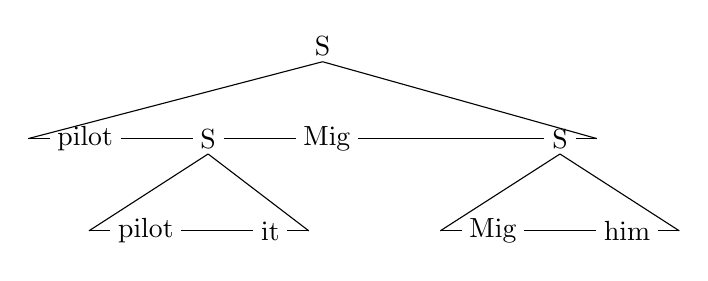
\begin{tikzpicture}
\node at (0.000000, 0.000000) {S};
\node at (-3.015490, -1.171530) {pilot};
\node at (-1.453439, -1.171530) {S};
\node at (-2.244228, -2.343060) {pilot};
\node at (-0.662651, -2.343060) {it};
\node at (0.054916, -1.171530) {Mig};
\node at (3.015490, -1.171530) {S};
\node at (2.163684, -2.343060) {Mig};
\node at (3.867296, -2.343060) {him};
\draw (0.000000,-0.195255) -- (-3.737938,-1.171530);
\draw (0.000000,-0.195255) -- (3.484105,-1.171530);
\draw (-3.737938,-1.171530) -- (-3.466951,-1.171530);
\draw (-2.564029,-1.171530) -- (-1.651067,-1.171530);
\draw (-1.255811,-1.171530) -- (-0.342850,-1.171530);
\draw (0.452681,-1.171530) -- (2.817862,-1.171530);
\draw (3.213118,-1.171530) -- (3.484105,-1.171530);
\draw (-1.453439,-1.366785) -- (-2.966676,-2.343060);
\draw (-1.453439,-1.366785) -- (-0.174510,-2.343060);
\draw (-2.966676,-2.343060) -- (-2.695689,-2.343060);
\draw (-1.792766,-2.343060) -- (-0.879805,-2.343060);
\draw (-0.445498,-2.343060) -- (-0.174510,-2.343060);
\draw (3.015490,-1.366785) -- (1.494932,-2.343060);
\draw (3.015490,-1.366785) -- (4.531167,-2.343060);
\draw (1.494932,-2.343060) -- (1.765919,-2.343060);
\draw (2.561450,-2.343060) -- (3.474411,-2.343060);
\draw (4.260180,-2.343060) -- (4.531167,-2.343060);
\end{tikzpicture}
}
\end{minipage}
\bigbreak

\bigbreak
\begin{minipage}{\textwidth}
  \makebox[\textwidth][c]{
  \begin{tabular}{|r|c|c|c|c|c|c|c|c|c|}
    \hline
    \multicolumn{10}{|c|}{\textbf{Features}} \\
    \hline
    & \textbf{\texttt{PNF}}
    & \textbf{\texttt{FPF}} & \textbf{\texttt{SPF}}
    & \textbf{\texttt{TPF}} & \textbf{\texttt{PLF}}
    & \textbf{\texttt{GNF}} & \textbf{\texttt{ANF}}
    & \textbf{\texttt{RPF}} & \textbf{\texttt{GEN}} \\
    \textbf{\texttt{pilot}} & \texttt{-}
    & \texttt{-} & \texttt{-}
    & \texttt{+} & \texttt{-}
    & \texttt{?} & \texttt{+}
    & \texttt{-} & \texttt{-} \\
    \textbf{\texttt{it}} & \texttt{+}
    & \texttt{-} & \texttt{-}
    & \texttt{+} & \texttt{-}
    & \texttt{?} & \texttt{-}
    & \texttt{-} & \texttt{-} \\
    \textbf{\texttt{Mig}} & \texttt{-}
    & \texttt{-} & \texttt{-}
    & \texttt{+} & \texttt{-}
    & \texttt{?} & \texttt{-}
    & \texttt{-} & \texttt{-} \\
    \textbf{\texttt{him}} & \texttt{+}
    & \texttt{-} & \texttt{-}
    & \texttt{+} & \texttt{-}
    & \texttt{-} & \texttt{+}
    & \texttt{-} & \texttt{-} \\
    \hline
  \end{tabular}
  }
\end{minipage}
\bigbreak

\bigbreak
\begin{minipage}{\textwidth}
  \makebox[\textwidth][c]{
  \begin{tabular}{|r|l|}
    \hline
    \multicolumn{2}{|c|}{\textbf{Nodes}} \\
    \hline
    ${\textbf{\textrm{1}}_{\phantom{z}}}$ & \texttt{\texttt{(S,~up:0,~dn:2,~lt:0,~rt:0,~th:2,~nu:1)}} \\
    ${\textbf{\textrm{2}}_{\phantom{z}}}$ & \texttt{\texttt{(N,~lit:pilot,~ftr:[---+-?+--],~up:1,~dn:0,}} \\
    & \texttt{\texttt{~lt:0,~rt:3,~th:3,~np:2,~ch:0,~co:${\textrm{2}_{\textrm{a}}}$,~ec:${\textrm{2}_{\textrm{b}}}$,}} \\
    & \texttt{\texttt{~pr:0,~su:5,~nu:2)}} \\
    ${\textbf{\textrm{2}}_{\textbf{\textrm{a}}}}$ & \texttt{\texttt{(E,~sub:A,~ftr:[---+-?+--],~np:2,~ch:0,~co:${\textrm{2}_{\textrm{b}}}$)}} \\
    ${\textbf{\textrm{2}}_{\textbf{\textrm{b}}}}$ & \texttt{\texttt{(E,~sub:B,~ftr:[---+--+--],~np:2,~ch:${\textrm{9}_{\textrm{a}}}$,~co:0)}} \\
    ${\textbf{\textrm{3}}_{\phantom{z}}}$ & \texttt{\texttt{(S,~up:1,~dn:4,~lt:2,~rt:6,~th:4,~nu:3)}} \\
    ${\textbf{\textrm{4}}_{\phantom{z}}}$ & \texttt{\texttt{(N,~lit:pilot,~ftr:[---+-?+--],~up:3,~dn:0,}} \\
    & \texttt{\texttt{~lt:0,~rt:5,~th:5,~np:4,~ch:0,~co:0,~ec:0,}} \\
    & \texttt{\texttt{~pr:0,~su:0,~nu:4)}} \\
    ${\textbf{\textrm{5}}_{\phantom{z}}}$ & \texttt{\texttt{(N,~lit:it,~ftr:[+--+-?---],~up:3,~dn:0,}} \\
    & \texttt{\texttt{~lt:4,~rt:0,~th:6,~np:5,~ch:0,~co:${\textrm{5}_{\textrm{a}}}$,~ec:${\textrm{5}_{\textrm{a}}}$,}} \\
    & \texttt{\texttt{~pr:2,~su:6,~nu:5)}} \\
    ${\textbf{\textrm{5}}_{\textbf{\textrm{a}}}}$ & \texttt{\texttt{(E,~sub:A,~ftr:[+--+-?---],~np:5,~ch:0,~co:0)}} \\
    ${\textbf{\textrm{6}}_{\phantom{z}}}$ & \texttt{\texttt{(N,~lit:Mig,~ftr:[---+-?---],~up:1,~dn:0,}} \\
    & \texttt{\texttt{~lt:3,~rt:7,~th:7,~np:6,~ch:0,~co:${\textrm{6}_{\textrm{a}}}$,~ec:${\textrm{6}_{\textrm{b}}}$,}} \\
    & \texttt{\texttt{~pr:5,~su:9,~nu:6)}} \\
    ${\textbf{\textrm{6}}_{\textbf{\textrm{a}}}}$ & \texttt{\texttt{(E,~sub:A,~ftr:[---+-?---],~np:6,~ch:0,~co:${\textrm{6}_{\textrm{b}}}$)}} \\
    ${\textbf{\textrm{6}}_{\textbf{\textrm{b}}}}$ & \texttt{\texttt{(E,~sub:B,~ftr:[---+-?---],~np:6,~ch:${\textrm{5}_{\textrm{a}}}$,~co:0)}} \\
    ${\textbf{\textrm{7}}_{\phantom{z}}}$ & \texttt{\texttt{(S,~up:1,~dn:8,~lt:6,~rt:0,~th:8,~nu:7)}} \\
    ${\textbf{\textrm{8}}_{\phantom{z}}}$ & \texttt{\texttt{(N,~lit:Mig,~ftr:[---+-?---],~up:7,~dn:0,}} \\
    & \texttt{\texttt{~lt:0,~rt:9,~th:9,~np:8,~ch:0,~co:0,~ec:0,}} \\
    & \texttt{\texttt{~pr:0,~su:0,~nu:8)}} \\
    ${\textbf{\textrm{9}}_{\phantom{z}}}$ & \texttt{\texttt{(N,~lit:him,~ftr:[+--+--+--],~up:7,~dn:0,}} \\
    & \texttt{\texttt{~lt:8,~rt:0,~th:0,~np:9,~ch:0,~co:${\textrm{9}_{\textrm{a}}}$,~ec:${\textrm{9}_{\textrm{a}}}$,}} \\
    & \texttt{\texttt{~pr:6,~su:0,~nu:9)}} \\
    ${\textbf{\textrm{9}}_{\textbf{\textrm{a}}}}$ & \texttt{\texttt{(E,~sub:A,~ftr:[+--+--+--],~np:9,~ch:0,~co:0)}} \\
    \hline
  \end{tabular}
  }
\end{minipage}
\bigbreak

\bigbreak
\begin{minipage}{\textwidth}
\makebox[\textwidth][c]{
\begin{tikzpicture}[
    every node/.style={align=center},
    dotted line/.style={draw, dotted, thick},
    curved arrow/.style={draw, thick, -{Latex[bend]}},
    ]
\node (S) at (2.790448,0.000000) {S};
\node (pilot) at (0.483259,-1.171530) {pilot};
\node (it) at (2.018131,-1.171530) {it};
\node (Mig) at (3.499307,-1.171530) {Mig};
\node (him) at (5.156214,-1.171530) {him};
\draw[dotted line] (S) -- (pilot);
\draw[dotted line] (S) -- (him);
\draw[dotted line] (pilot) -- (it);
\draw[dotted line] (it) -- (Mig);
\draw[dotted line] (Mig) -- (him);
\node (pilotA) at (0.483259,-2.343060) {${\textrm{pilot}_{\textrm{a}}}$};
\node (itA) at (2.018131,-2.343060) {${\textrm{it}_{\textrm{a}}}$};
\node (MigA) at (3.499307,-2.343060) {${\textrm{Mig}_{\textrm{a}}}$};
\node (himA) at (5.156214,-2.343060) {${\textrm{him}_{\textrm{a}}}$};
\draw[dotted line] (pilot) -- (pilotA);
\draw[dotted line] (it) -- (itA);
\draw[dotted line] (Mig) -- (MigA);
\draw[dotted line] (him) -- (himA);
\node (pilotB) at (0.483259,-3.514590) {${\textrm{pilot}_{\textrm{b}}}$};
\node (MigB) at (3.499307,-3.514590) {${\textrm{Mig}_{\textrm{b}}}$};
\draw[dotted line] (pilotA) -- (pilotB);
\draw[dotted line] (MigA) -- (MigB);
\draw[curved arrow] (pilotB.north east) to [out=28.62,in=-151.38] (himA.south west);
\draw[curved arrow] (MigB.north west) to [out=121.41,in=-58.59] (itA.south east);
\end{tikzpicture}
}
\end{minipage}
\bigbreak

\bigbreak
\begin{minipage}{\textwidth}
  \makebox[\textwidth][c]{
  \begin{tabular}{|l|l|l|l|}
    \hline
    \multicolumn{4}{|c|}{\textbf{Chaining}} \\
    \hline
    \textbf{\texttt{pilot}} & \textbf{\texttt{it}}
    & \textbf{\texttt{Mig}} & \textbf{\texttt{him}} \\
    ${\texttt{pilot}_{\texttt{a}}}$ & ${\texttt{it}_{\texttt{a}}}$
    & ${\texttt{Mig}_{\texttt{a}}}$ & ${\texttt{him}_{\texttt{a}}}$ \\
    ${\texttt{pilot}_{\texttt{b}}}$\texttt{\symbol{94}}${\texttt{him}_{\texttt{a}}}$ & 
    & ${\texttt{Mig}_{\texttt{b}}}$\texttt{\symbol{94}}${\texttt{it}_{\texttt{a}}}$ &  \\
    \hline
  \end{tabular}
  }
\end{minipage}
\bigbreak

\bigbreak
\begin{minipage}{\textwidth}
  \makebox[\textwidth][c]{
  \begin{tabular}{|c|}
    \hline
    \multicolumn{1}{|c|}{\textbf{Interpretations}} \\
    \hline
    ${\texttt{Mig}_{\texttt{b}}}$\texttt{\symbol{94}}${\texttt{it}_{\texttt{a}}}$\qquad ${\texttt{pilot}_{\texttt{b}}}$\texttt{\symbol{94}}${\texttt{him}_{\texttt{a}}}$ \\
    \hline
  \end{tabular}
  }
\end{minipage}
\bigbreak

\clearpage

%%%%%%%%%%%%%%%%%%%%%%%%%%%%%%%%%%%%%%%%%%%%%%%%%%%%%%%%%%%%%%%%
%
%     (1.86) The mosquito which bit Algernon was killed by him.
%
%%%%%%%%%%%%%%%%%%%%%%%%%%%%%%%%%%%%%%%%%%%%%%%%%%%%%%%%%%%%%%%%

\section*{(1.86) The mosquito which bit Algernon was killed by him.}
\addcontentsline{toc}{section}{(1.86) The mosquito which bit Algernon was killed by him.}

\bigbreak
\begin{enumerate*}
\item[(1.86)] The mosquito which bit Algernon was killed by him.
\end{enumerate*}
\bigbreak
\bigbreak
\begin{minipage}{\textwidth}
\makebox[\textwidth][c]{
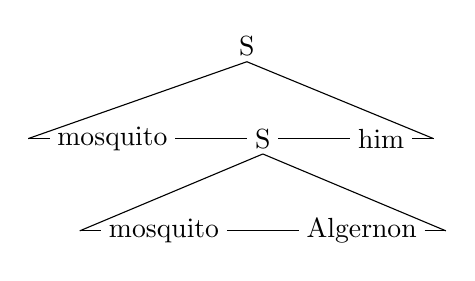
\begin{tikzpicture}
\node at (0.000000, 0.000000) {S};
\node at (-1.706540, -1.171530) {mosquito};
\node at (0.203066, -1.171530) {S};
\node at (-1.052187, -2.343060) {mosquito};
\node at (1.458320, -2.343060) {Algernon};
\node at (1.706540, -1.171530) {him};
\draw (0.000000,-0.195255) -- (-2.776544,-1.171530);
\draw (0.000000,-0.195255) -- (2.370411,-1.171530);
\draw (-2.776544,-1.171530) -- (-2.505557,-1.171530);
\draw (-0.907523,-1.171530) -- (0.005438,-1.171530);
\draw (0.400694,-1.171530) -- (1.313656,-1.171530);
\draw (2.099424,-1.171530) -- (2.370411,-1.171530);
\draw (0.203066,-1.366785) -- (-2.122191,-2.343060);
\draw (0.203066,-1.366785) -- (2.527835,-2.343060);
\draw (-2.122191,-2.343060) -- (-1.851204,-2.343060);
\draw (-0.253170,-2.343060) -- (0.659791,-2.343060);
\draw (2.256848,-2.343060) -- (2.527835,-2.343060);
\end{tikzpicture}
}
\end{minipage}
\bigbreak

\bigbreak
\begin{minipage}{\textwidth}
  \makebox[\textwidth][c]{
  \begin{tabular}{|r|c|c|c|c|c|c|c|c|c|}
    \hline
    \multicolumn{10}{|c|}{\textbf{Features}} \\
    \hline
    & \textbf{\texttt{PNF}}
    & \textbf{\texttt{FPF}} & \textbf{\texttt{SPF}}
    & \textbf{\texttt{TPF}} & \textbf{\texttt{PLF}}
    & \textbf{\texttt{GNF}} & \textbf{\texttt{ANF}}
    & \textbf{\texttt{RPF}} & \textbf{\texttt{GEN}} \\
    \textbf{\texttt{mosquito}} & \texttt{-}
    & \texttt{-} & \texttt{-}
    & \texttt{+} & \texttt{-}
    & \texttt{?} & \texttt{+}
    & \texttt{-} & \texttt{-} \\
    \textbf{\texttt{Algernon}} & \texttt{-}
    & \texttt{-} & \texttt{-}
    & \texttt{+} & \texttt{-}
    & \texttt{-} & \texttt{+}
    & \texttt{-} & \texttt{-} \\
    \textbf{\texttt{him}} & \texttt{+}
    & \texttt{-} & \texttt{-}
    & \texttt{+} & \texttt{-}
    & \texttt{-} & \texttt{+}
    & \texttt{-} & \texttt{-} \\
    \hline
  \end{tabular}
  }
\end{minipage}
\bigbreak

\bigbreak
\begin{minipage}{\textwidth}
  \makebox[\textwidth][c]{
  \begin{tabular}{|r|l|}
    \hline
    \multicolumn{2}{|c|}{\textbf{Nodes}} \\
    \hline
    ${\textbf{\textrm{1}}_{\phantom{z}}}$ & \texttt{\texttt{(S,~up:0,~dn:2,~lt:0,~rt:0,~th:2,~nu:1)}} \\
    ${\textbf{\textrm{2}}_{\phantom{z}}}$ & \texttt{\texttt{(N,~lit:mosquito,~ftr:[---+-?+--],~up:1,~dn:0,}} \\
    & \texttt{\texttt{~lt:0,~rt:3,~th:3,~np:2,~ch:0,~co:${\textrm{2}_{\textrm{a}}}$,~ec:${\textrm{2}_{\textrm{a}}}$,}} \\
    & \texttt{\texttt{~pr:0,~su:5,~nu:2)}} \\
    ${\textbf{\textrm{2}}_{\textbf{\textrm{a}}}}$ & \texttt{\texttt{(E,~sub:A,~ftr:[---+-?+--],~np:2,~ch:0,~co:0)}} \\
    ${\textbf{\textrm{3}}_{\phantom{z}}}$ & \texttt{\texttt{(S,~up:1,~dn:4,~lt:2,~rt:6,~th:4,~nu:3)}} \\
    ${\textbf{\textrm{4}}_{\phantom{z}}}$ & \texttt{\texttt{(N,~lit:mosquito,~ftr:[---+-?+--],~up:3,~dn:0,}} \\
    & \texttt{\texttt{~lt:0,~rt:5,~th:5,~np:4,~ch:0,~co:0,~ec:0,}} \\
    & \texttt{\texttt{~pr:0,~su:0,~nu:4)}} \\
    ${\textbf{\textrm{5}}_{\phantom{z}}}$ & \texttt{\texttt{(N,~lit:Algernon,~ftr:[---+--+--],~up:3,~dn:0,}} \\
    & \texttt{\texttt{~lt:4,~rt:0,~th:6,~np:5,~ch:0,~co:${\textrm{5}_{\textrm{a}}}$,~ec:${\textrm{5}_{\textrm{b}}}$,}} \\
    & \texttt{\texttt{~pr:2,~su:6,~nu:5)}} \\
    ${\textbf{\textrm{5}}_{\textbf{\textrm{a}}}}$ & \texttt{\texttt{(E,~sub:A,~ftr:[---+--+--],~np:5,~ch:0,~co:${\textrm{5}_{\textrm{b}}}$)}} \\
    ${\textbf{\textrm{5}}_{\textbf{\textrm{b}}}}$ & \texttt{\texttt{(E,~sub:B,~ftr:[---+--+--],~np:5,~ch:${\textrm{6}_{\textrm{a}}}$,~co:0)}} \\
    ${\textbf{\textrm{6}}_{\phantom{z}}}$ & \texttt{\texttt{(N,~lit:him,~ftr:[+--+--+--],~up:1,~dn:0,}} \\
    & \texttt{\texttt{~lt:3,~rt:0,~th:0,~np:6,~ch:0,~co:${\textrm{6}_{\textrm{a}}}$,~ec:${\textrm{6}_{\textrm{a}}}$,}} \\
    & \texttt{\texttt{~pr:5,~su:0,~nu:6)}} \\
    ${\textbf{\textrm{6}}_{\textbf{\textrm{a}}}}$ & \texttt{\texttt{(E,~sub:A,~ftr:[+--+--+--],~np:6,~ch:0,~co:0)}} \\
    \hline
  \end{tabular}
  }
\end{minipage}
\bigbreak

\bigbreak
\begin{minipage}{\textwidth}
\makebox[\textwidth][c]{
\begin{tikzpicture}[
    every node/.style={align=center},
    dotted line/.style={draw, dotted, thick},
    curved arrow/.style={draw, thick, -{Latex[bend]}},
    ]
\node (S) at (2.888484,0.000000) {S};
\node (mosquito) at (0.830815,-1.171530) {mosquito};
\node (Algernon) at (3.294617,-1.171530) {Algernon};
\node (him) at (5.352286,-1.171530) {him};
\draw[dotted line] (S) -- (mosquito);
\draw[dotted line] (S) -- (him);
\draw[dotted line] (mosquito) -- (Algernon);
\draw[dotted line] (Algernon) -- (him);
\node (mosquitoA) at (0.830815,-2.343060) {${\textrm{mosquito}_{\textrm{a}}}$};
\node (AlgernonA) at (3.294617,-2.343060) {${\textrm{Algernon}_{\textrm{a}}}$};
\node (himA) at (5.352286,-2.343060) {${\textrm{him}_{\textrm{a}}}$};
\draw[dotted line] (mosquito) -- (mosquitoA);
\draw[dotted line] (Algernon) -- (AlgernonA);
\draw[dotted line] (him) -- (himA);
\node (AlgernonB) at (3.294617,-3.514590) {${\textrm{Algernon}_{\textrm{b}}}$};
\draw[dotted line] (AlgernonA) -- (AlgernonB);
\draw[curved arrow] (AlgernonB.north east) to [out=58.59,in=-121.41] (himA.south west);
\end{tikzpicture}
}
\end{minipage}
\bigbreak

\bigbreak
\begin{minipage}{\textwidth}
  \makebox[\textwidth][c]{
  \begin{tabular}{|l|l|l|}
    \hline
    \multicolumn{3}{|c|}{\textbf{Chaining}} \\
    \hline
    \textbf{\texttt{mosquito}} & \textbf{\texttt{Algernon}}
    & \textbf{\texttt{him}} \\
    ${\texttt{mosquito}_{\texttt{a}}}$ & ${\texttt{Algernon}_{\texttt{a}}}$
    & ${\texttt{him}_{\texttt{a}}}$ \\
     & ${\texttt{Algernon}_{\texttt{b}}}$\texttt{\symbol{94}}${\texttt{him}_{\texttt{a}}}$
    &  \\
    \hline
  \end{tabular}
  }
\end{minipage}
\bigbreak

\bigbreak
\begin{minipage}{\textwidth}
  \makebox[\textwidth][c]{
  \begin{tabular}{|c|}
    \hline
    \multicolumn{1}{|c|}{\textbf{Interpretations}} \\
    \hline
    ${\texttt{Algernon}_{\texttt{b}}}$\texttt{\symbol{94}}${\texttt{him}_{\texttt{a}}}$ \\
    \hline
  \end{tabular}
  }
\end{minipage}
\bigbreak

\clearpage

%%%%%%%%%%%%%%%%%%%%%%%%%%%%%%%%%%%%%%%%%%%%%%%%%%%%%%%%%%%%%%%%
%
%     (1.87) The mosquito which bit him was killed by Algernon.
%
%%%%%%%%%%%%%%%%%%%%%%%%%%%%%%%%%%%%%%%%%%%%%%%%%%%%%%%%%%%%%%%%

\section*{(1.87) The mosquito which bit him was killed by Algernon.}
\addcontentsline{toc}{section}{(1.87) The mosquito which bit him was killed by Algernon.}

\bigbreak
\begin{enumerate*}
\item[(1.87)] The mosquito which bit him was killed by Algernon.
\end{enumerate*}
\bigbreak
\bigbreak
\begin{minipage}{\textwidth}
\makebox[\textwidth][c]{
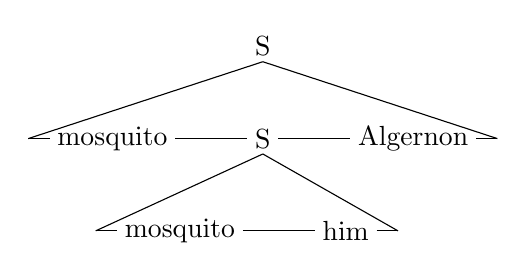
\begin{tikzpicture}
\node at (0.000000, 0.000000) {S};
\node at (-1.909362, -1.171530) {mosquito};
\node at (0.000244, -1.171530) {S};
\node at (-1.052187, -2.343060) {mosquito};
\node at (1.052675, -2.343060) {him};
\node at (1.909362, -1.171530) {Algernon};
\draw (0.000000,-0.195255) -- (-2.979366,-1.171530);
\draw (0.000000,-0.195255) -- (2.978878,-1.171530);
\draw (-2.979366,-1.171530) -- (-2.708379,-1.171530);
\draw (-1.110345,-1.171530) -- (-0.197384,-1.171530);
\draw (0.197872,-1.171530) -- (1.110834,-1.171530);
\draw (2.707891,-1.171530) -- (2.978878,-1.171530);
\draw (0.000244,-1.366785) -- (-2.122191,-2.343060);
\draw (0.000244,-1.366785) -- (1.716547,-2.343060);
\draw (-2.122191,-2.343060) -- (-1.851204,-2.343060);
\draw (-0.253170,-2.343060) -- (0.659791,-2.343060);
\draw (1.445560,-2.343060) -- (1.716547,-2.343060);
\end{tikzpicture}
}
\end{minipage}
\bigbreak

\bigbreak
\begin{minipage}{\textwidth}
  \makebox[\textwidth][c]{
  \begin{tabular}{|r|c|c|c|c|c|c|c|c|c|}
    \hline
    \multicolumn{10}{|c|}{\textbf{Features}} \\
    \hline
    & \textbf{\texttt{PNF}}
    & \textbf{\texttt{FPF}} & \textbf{\texttt{SPF}}
    & \textbf{\texttt{TPF}} & \textbf{\texttt{PLF}}
    & \textbf{\texttt{GNF}} & \textbf{\texttt{ANF}}
    & \textbf{\texttt{RPF}} & \textbf{\texttt{GEN}} \\
    \textbf{\texttt{mosquito}} & \texttt{-}
    & \texttt{-} & \texttt{-}
    & \texttt{+} & \texttt{-}
    & \texttt{?} & \texttt{+}
    & \texttt{-} & \texttt{-} \\
    \textbf{\texttt{him}} & \texttt{+}
    & \texttt{-} & \texttt{-}
    & \texttt{+} & \texttt{-}
    & \texttt{-} & \texttt{+}
    & \texttt{-} & \texttt{-} \\
    \textbf{\texttt{Algernon}} & \texttt{-}
    & \texttt{-} & \texttt{-}
    & \texttt{+} & \texttt{-}
    & \texttt{-} & \texttt{+}
    & \texttt{-} & \texttt{-} \\
    \hline
  \end{tabular}
  }
\end{minipage}
\bigbreak

\bigbreak
\begin{minipage}{\textwidth}
  \makebox[\textwidth][c]{
  \begin{tabular}{|r|l|}
    \hline
    \multicolumn{2}{|c|}{\textbf{Nodes}} \\
    \hline
    ${\textbf{\textrm{1}}_{\phantom{z}}}$ & \texttt{\texttt{(S,~up:0,~dn:2,~lt:0,~rt:0,~th:2,~nu:1)}} \\
    ${\textbf{\textrm{2}}_{\phantom{z}}}$ & \texttt{\texttt{(N,~lit:mosquito,~ftr:[---+-?+--],~up:1,~dn:0,}} \\
    & \texttt{\texttt{~lt:0,~rt:3,~th:3,~np:2,~ch:0,~co:${\textrm{2}_{\textrm{a}}}$,~ec:${\textrm{2}_{\textrm{b}}}$,}} \\
    & \texttt{\texttt{~pr:0,~su:5,~nu:2)}} \\
    ${\textbf{\textrm{2}}_{\textbf{\textrm{a}}}}$ & \texttt{\texttt{(E,~sub:A,~ftr:[---+-?+--],~np:2,~ch:0,~co:${\textrm{2}_{\textrm{b}}}$)}} \\
    ${\textbf{\textrm{2}}_{\textbf{\textrm{b}}}}$ & \texttt{\texttt{(E,~sub:B,~ftr:[---+--+--],~np:2,~ch:${\textrm{5}_{\textrm{a}}}$,~co:0)}} \\
    ${\textbf{\textrm{3}}_{\phantom{z}}}$ & \texttt{\texttt{(S,~up:1,~dn:4,~lt:2,~rt:6,~th:4,~nu:3)}} \\
    ${\textbf{\textrm{4}}_{\phantom{z}}}$ & \texttt{\texttt{(N,~lit:mosquito,~ftr:[---+-?+--],~up:3,~dn:0,}} \\
    & \texttt{\texttt{~lt:0,~rt:5,~th:5,~np:4,~ch:0,~co:0,~ec:0,}} \\
    & \texttt{\texttt{~pr:0,~su:0,~nu:4)}} \\
    ${\textbf{\textrm{5}}_{\phantom{z}}}$ & \texttt{\texttt{(N,~lit:him,~ftr:[+--+--+--],~up:3,~dn:0,}} \\
    & \texttt{\texttt{~lt:4,~rt:0,~th:6,~np:5,~ch:0,~co:${\textrm{5}_{\textrm{a}}}$,~ec:${\textrm{5}_{\textrm{a}}}$,}} \\
    & \texttt{\texttt{~pr:2,~su:6,~nu:5)}} \\
    ${\textbf{\textrm{5}}_{\textbf{\textrm{a}}}}$ & \texttt{\texttt{(E,~sub:A,~ftr:[+--+--+--],~np:5,~ch:0,~co:0)}} \\
    ${\textbf{\textrm{6}}_{\phantom{z}}}$ & \texttt{\texttt{(N,~lit:Algernon,~ftr:[---+--+--],~up:1,~dn:0,}} \\
    & \texttt{\texttt{~lt:3,~rt:0,~th:0,~np:6,~ch:0,~co:${\textrm{6}_{\textrm{a}}}$,~ec:${\textrm{6}_{\textrm{b}}}$,}} \\
    & \texttt{\texttt{~pr:5,~su:0,~nu:6)}} \\
    ${\textbf{\textrm{6}}_{\textbf{\textrm{a}}}}$ & \texttt{\texttt{(E,~sub:A,~ftr:[---+--+--],~np:6,~ch:0,~co:${\textrm{6}_{\textrm{b}}}$)}} \\
    ${\textbf{\textrm{6}}_{\textbf{\textrm{b}}}}$ & \texttt{\texttt{(E,~sub:B,~ftr:[---+--+--],~np:6,~ch:${\textrm{5}_{\textrm{a}}}$,~co:0)}} \\
    \hline
  \end{tabular}
  }
\end{minipage}
\bigbreak

\bigbreak
\begin{minipage}{\textwidth}
\makebox[\textwidth][c]{
\begin{tikzpicture}[
    every node/.style={align=center},
    dotted line/.style={draw, dotted, thick},
    curved arrow/.style={draw, thick, -{Latex[bend]}},
    ]
\node (S) at (2.888484,0.000000) {S};
\node (mosquito) at (0.830815,-1.171530) {mosquito};
\node (him) at (2.888973,-1.171530) {him};
\node (Algernon) at (4.946642,-1.171530) {Algernon};
\draw[dotted line] (S) -- (mosquito);
\draw[dotted line] (S) -- (Algernon);
\draw[dotted line] (mosquito) -- (him);
\draw[dotted line] (him) -- (Algernon);
\node (mosquitoA) at (0.830815,-2.343060) {${\textrm{mosquito}_{\textrm{a}}}$};
\node (himA) at (2.888973,-2.343060) {${\textrm{him}_{\textrm{a}}}$};
\node (AlgernonA) at (4.946642,-2.343060) {${\textrm{Algernon}_{\textrm{a}}}$};
\draw[dotted line] (mosquito) -- (mosquitoA);
\draw[dotted line] (him) -- (himA);
\draw[dotted line] (Algernon) -- (AlgernonA);
\node (mosquitoB) at (0.830815,-3.514590) {${\textrm{mosquito}_{\textrm{b}}}$};
\node (AlgernonB) at (4.946642,-3.514590) {${\textrm{Algernon}_{\textrm{b}}}$};
\draw[dotted line] (mosquitoA) -- (mosquitoB);
\draw[dotted line] (AlgernonA) -- (AlgernonB);
\draw[curved arrow] (AlgernonB.north west) to [out=121.41,in=-29.29] (himA.south east);
\draw[curved arrow] (mosquitoB.north east) to [out=58.59,in=-150.71] (himA.south west);
\end{tikzpicture}
}
\end{minipage}
\bigbreak

\bigbreak
\begin{minipage}{\textwidth}
  \makebox[\textwidth][c]{
  \begin{tabular}{|l|l|l|}
    \hline
    \multicolumn{3}{|c|}{\textbf{Chaining}} \\
    \hline
    \textbf{\texttt{mosquito}} & \textbf{\texttt{him}}
    & \textbf{\texttt{Algernon}} \\
    ${\texttt{mosquito}_{\texttt{a}}}$ & ${\texttt{him}_{\texttt{a}}}$
    & ${\texttt{Algernon}_{\texttt{a}}}$ \\
    ${\texttt{mosquito}_{\texttt{b}}}$\texttt{\symbol{94}}${\texttt{him}_{\texttt{a}}}$ & 
    & ${\texttt{Algernon}_{\texttt{b}}}$\texttt{\symbol{94}}${\texttt{him}_{\texttt{a}}}$ \\
    \hline
  \end{tabular}
  }
\end{minipage}
\bigbreak

\bigbreak
\begin{minipage}{\textwidth}
  \makebox[\textwidth][c]{
  \begin{tabular}{|c|}
    \hline
    \multicolumn{1}{|c|}{\textbf{Interpretations}} \\
    \hline
    ${\texttt{mosquito}_{\texttt{b}}}$\texttt{\symbol{94}}${\texttt{him}_{\texttt{a}}}$ \\
    \hline
    ${\texttt{Algernon}_{\texttt{b}}}$\texttt{\symbol{94}}${\texttt{him}_{\texttt{a}}}$ \\
    \hline
  \end{tabular}
  }
\end{minipage}
\bigbreak

\clearpage

%%%%%%%%%%%%%%%%%%%%%%%%%%%%%%%%%%%%%%%%%%%%%%%%%%%%%%%%%%%%%%%%
%
%     (1.88) Algernon killed the mosquito which bit him.
%
%%%%%%%%%%%%%%%%%%%%%%%%%%%%%%%%%%%%%%%%%%%%%%%%%%%%%%%%%%%%%%%%

\section*{(1.88) Algernon killed the mosquito which bit him.}
\addcontentsline{toc}{section}{(1.88) Algernon killed the mosquito which bit him.}

\bigbreak
\begin{enumerate*}
\item[(1.88)] Algernon killed the mosquito which bit him.
\end{enumerate*}
\bigbreak
\bigbreak
\begin{minipage}{\textwidth}
\makebox[\textwidth][c]{
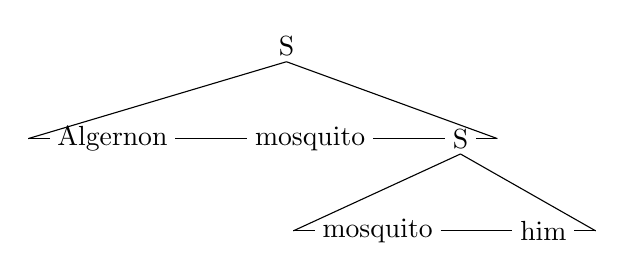
\begin{tikzpicture}
\node at (0.000000, 0.000000) {S};
\node at (-2.210056, -1.171530) {Algernon};
\node at (0.300450, -1.171530) {mosquito};
\node at (2.210056, -1.171530) {S};
\node at (1.157625, -2.343060) {mosquito};
\node at (3.262488, -2.343060) {him};
\draw (0.000000,-0.195255) -- (-3.279572,-1.171530);
\draw (0.000000,-0.195255) -- (2.678672,-1.171530);
\draw (-3.279572,-1.171530) -- (-3.008585,-1.171530);
\draw (-1.411528,-1.171530) -- (-0.498567,-1.171530);
\draw (1.099467,-1.171530) -- (2.012428,-1.171530);
\draw (2.407685,-1.171530) -- (2.678672,-1.171530);
\draw (2.210056,-1.366785) -- (0.087621,-2.343060);
\draw (2.210056,-1.366785) -- (3.926359,-2.343060);
\draw (0.087621,-2.343060) -- (0.358608,-2.343060);
\draw (1.956642,-2.343060) -- (2.869603,-2.343060);
\draw (3.655372,-2.343060) -- (3.926359,-2.343060);
\end{tikzpicture}
}
\end{minipage}
\bigbreak

\bigbreak
\begin{minipage}{\textwidth}
  \makebox[\textwidth][c]{
  \begin{tabular}{|r|c|c|c|c|c|c|c|c|c|}
    \hline
    \multicolumn{10}{|c|}{\textbf{Features}} \\
    \hline
    & \textbf{\texttt{PNF}}
    & \textbf{\texttt{FPF}} & \textbf{\texttt{SPF}}
    & \textbf{\texttt{TPF}} & \textbf{\texttt{PLF}}
    & \textbf{\texttt{GNF}} & \textbf{\texttt{ANF}}
    & \textbf{\texttt{RPF}} & \textbf{\texttt{GEN}} \\
    \textbf{\texttt{Algernon}} & \texttt{-}
    & \texttt{-} & \texttt{-}
    & \texttt{+} & \texttt{-}
    & \texttt{-} & \texttt{+}
    & \texttt{-} & \texttt{-} \\
    \textbf{\texttt{mosquito}} & \texttt{-}
    & \texttt{-} & \texttt{-}
    & \texttt{+} & \texttt{-}
    & \texttt{?} & \texttt{+}
    & \texttt{-} & \texttt{-} \\
    \textbf{\texttt{him}} & \texttt{+}
    & \texttt{-} & \texttt{-}
    & \texttt{+} & \texttt{-}
    & \texttt{-} & \texttt{+}
    & \texttt{-} & \texttt{-} \\
    \hline
  \end{tabular}
  }
\end{minipage}
\bigbreak

\bigbreak
\begin{minipage}{\textwidth}
  \makebox[\textwidth][c]{
  \begin{tabular}{|r|l|}
    \hline
    \multicolumn{2}{|c|}{\textbf{Nodes}} \\
    \hline
    ${\textbf{\textrm{1}}_{\phantom{z}}}$ & \texttt{\texttt{(S,~up:0,~dn:2,~lt:0,~rt:0,~th:2,~nu:1)}} \\
    ${\textbf{\textrm{2}}_{\phantom{z}}}$ & \texttt{\texttt{(N,~lit:Algernon,~ftr:[---+--+--],~up:1,~dn:0,}} \\
    & \texttt{\texttt{~lt:0,~rt:3,~th:3,~np:2,~ch:0,~co:${\textrm{2}_{\textrm{a}}}$,~ec:${\textrm{2}_{\textrm{b}}}$,}} \\
    & \texttt{\texttt{~pr:0,~su:3,~nu:2)}} \\
    ${\textbf{\textrm{2}}_{\textbf{\textrm{a}}}}$ & \texttt{\texttt{(E,~sub:A,~ftr:[---+--+--],~np:2,~ch:0,~co:${\textrm{2}_{\textrm{b}}}$)}} \\
    ${\textbf{\textrm{2}}_{\textbf{\textrm{b}}}}$ & \texttt{\texttt{(E,~sub:B,~ftr:[---+--+--],~np:2,~ch:${\textrm{6}_{\textrm{a}}}$,~co:0)}} \\
    ${\textbf{\textrm{3}}_{\phantom{z}}}$ & \texttt{\texttt{(N,~lit:mosquito,~ftr:[---+-?+--],~up:1,~dn:0,}} \\
    & \texttt{\texttt{~lt:2,~rt:4,~th:4,~np:3,~ch:0,~co:${\textrm{3}_{\textrm{a}}}$,~ec:${\textrm{3}_{\textrm{b}}}$,}} \\
    & \texttt{\texttt{~pr:2,~su:6,~nu:3)}} \\
    ${\textbf{\textrm{3}}_{\textbf{\textrm{a}}}}$ & \texttt{\texttt{(E,~sub:A,~ftr:[---+-?+--],~np:3,~ch:0,~co:${\textrm{3}_{\textrm{b}}}$)}} \\
    ${\textbf{\textrm{3}}_{\textbf{\textrm{b}}}}$ & \texttt{\texttt{(E,~sub:B,~ftr:[---+--+--],~np:3,~ch:${\textrm{6}_{\textrm{a}}}$,~co:0)}} \\
    ${\textbf{\textrm{4}}_{\phantom{z}}}$ & \texttt{\texttt{(S,~up:1,~dn:5,~lt:3,~rt:0,~th:5,~nu:4)}} \\
    ${\textbf{\textrm{5}}_{\phantom{z}}}$ & \texttt{\texttt{(N,~lit:mosquito,~ftr:[---+-?+--],~up:4,~dn:0,}} \\
    & \texttt{\texttt{~lt:0,~rt:6,~th:6,~np:5,~ch:0,~co:0,~ec:0,}} \\
    & \texttt{\texttt{~pr:0,~su:0,~nu:5)}} \\
    ${\textbf{\textrm{6}}_{\phantom{z}}}$ & \texttt{\texttt{(N,~lit:him,~ftr:[+--+--+--],~up:4,~dn:0,}} \\
    & \texttt{\texttt{~lt:5,~rt:0,~th:0,~np:6,~ch:0,~co:${\textrm{6}_{\textrm{a}}}$,~ec:${\textrm{6}_{\textrm{a}}}$,}} \\
    & \texttt{\texttt{~pr:3,~su:0,~nu:6)}} \\
    ${\textbf{\textrm{6}}_{\textbf{\textrm{a}}}}$ & \texttt{\texttt{(E,~sub:A,~ftr:[+--+--+--],~np:6,~ch:0,~co:0)}} \\
    \hline
  \end{tabular}
  }
\end{minipage}
\bigbreak

\bigbreak
\begin{minipage}{\textwidth}
\makebox[\textwidth][c]{
\begin{tikzpicture}[
    every node/.style={align=center},
    dotted line/.style={draw, dotted, thick},
    curved arrow/.style={draw, thick, -{Latex[bend]}},
    ]
\node (S) at (2.888484,0.000000) {S};
\node (Algernon) at (0.830326,-1.171530) {Algernon};
\node (mosquito) at (3.294128,-1.171530) {mosquito};
\node (him) at (5.352286,-1.171530) {him};
\draw[dotted line] (S) -- (Algernon);
\draw[dotted line] (S) -- (him);
\draw[dotted line] (Algernon) -- (mosquito);
\draw[dotted line] (mosquito) -- (him);
\node (AlgernonA) at (0.830326,-2.343060) {${\textrm{Algernon}_{\textrm{a}}}$};
\node (mosquitoA) at (3.294128,-2.343060) {${\textrm{mosquito}_{\textrm{a}}}$};
\node (himA) at (5.352286,-2.343060) {${\textrm{him}_{\textrm{a}}}$};
\draw[dotted line] (Algernon) -- (AlgernonA);
\draw[dotted line] (mosquito) -- (mosquitoA);
\draw[dotted line] (him) -- (himA);
\node (AlgernonB) at (0.830326,-3.514590) {${\textrm{Algernon}_{\textrm{b}}}$};
\node (mosquitoB) at (3.294128,-3.514590) {${\textrm{mosquito}_{\textrm{b}}}$};
\draw[dotted line] (AlgernonA) -- (AlgernonB);
\draw[dotted line] (mosquitoA) -- (mosquitoB);
\draw[curved arrow] (mosquitoB.north east) to [out=58.59,in=-81.23] (himA.south);
\draw[curved arrow] (AlgernonB.north east) to [out=39.31,in=179.13] (himA.west);
\end{tikzpicture}
}
\end{minipage}
\bigbreak

\bigbreak
\begin{minipage}{\textwidth}
  \makebox[\textwidth][c]{
  \begin{tabular}{|l|l|l|}
    \hline
    \multicolumn{3}{|c|}{\textbf{Chaining}} \\
    \hline
    \textbf{\texttt{Algernon}} & \textbf{\texttt{mosquito}}
    & \textbf{\texttt{him}} \\
    ${\texttt{Algernon}_{\texttt{a}}}$ & ${\texttt{mosquito}_{\texttt{a}}}$
    & ${\texttt{him}_{\texttt{a}}}$ \\
    ${\texttt{Algernon}_{\texttt{b}}}$\texttt{\symbol{94}}${\texttt{him}_{\texttt{a}}}$ & ${\texttt{mosquito}_{\texttt{b}}}$\texttt{\symbol{94}}${\texttt{him}_{\texttt{a}}}$
    &  \\
    \hline
  \end{tabular}
  }
\end{minipage}
\bigbreak

\bigbreak
\begin{minipage}{\textwidth}
  \makebox[\textwidth][c]{
  \begin{tabular}{|c|}
    \hline
    \multicolumn{1}{|c|}{\textbf{Interpretations}} \\
    \hline
    ${\texttt{Algernon}_{\texttt{b}}}$\texttt{\symbol{94}}${\texttt{him}_{\texttt{a}}}$ \\
    \hline
    ${\texttt{mosquito}_{\texttt{b}}}$\texttt{\symbol{94}}${\texttt{him}_{\texttt{a}}}$ \\
    \hline
  \end{tabular}
  }
\end{minipage}
\bigbreak

\clearpage

%%%%%%%%%%%%%%%%%%%%%%%%%%%%%%%%%%%%%%%%%%%%%%%%%%%%%%%%%%%%%%%%
%
%     (1.89) He killed the mosquito which bit Algernon.
%
%%%%%%%%%%%%%%%%%%%%%%%%%%%%%%%%%%%%%%%%%%%%%%%%%%%%%%%%%%%%%%%%

\section*{(1.89) He killed the mosquito which bit Algernon.}
\addcontentsline{toc}{section}{(1.89) He killed the mosquito which bit Algernon.}

\bigbreak
\begin{enumerate*}
\item[(1.89)] He killed the mosquito which bit Algernon.
\end{enumerate*}
\bigbreak
\bigbreak
\begin{minipage}{\textwidth}
\makebox[\textwidth][c]{
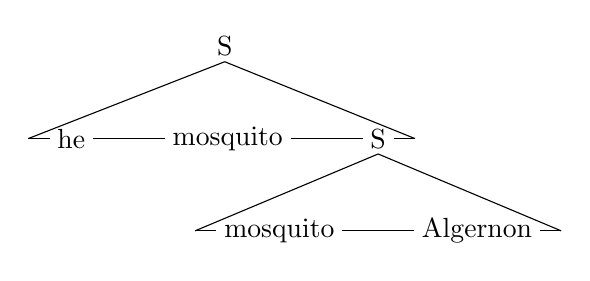
\begin{tikzpicture}
\node at (0.000000, 0.000000) {S};
\node at (-1.948657, -1.171530) {he};
\node at (0.039051, -1.171530) {mosquito};
\node at (1.948657, -1.171530) {S};
\node at (0.693404, -2.343060) {mosquito};
\node at (3.203911, -2.343060) {Algernon};
\draw (0.000000,-0.195255) -- (-2.495375,-1.171530);
\draw (0.000000,-0.195255) -- (2.417272,-1.171530);
\draw (-2.495375,-1.171530) -- (-2.224387,-1.171530);
\draw (-1.672927,-1.171530) -- (-0.759966,-1.171530);
\draw (0.838068,-1.171530) -- (1.751029,-1.171530);
\draw (2.146285,-1.171530) -- (2.417272,-1.171530);
\draw (1.948657,-1.366785) -- (-0.376600,-2.343060);
\draw (1.948657,-1.366785) -- (4.273426,-2.343060);
\draw (-0.376600,-2.343060) -- (-0.105613,-2.343060);
\draw (1.492421,-2.343060) -- (2.405382,-2.343060);
\draw (4.002439,-2.343060) -- (4.273426,-2.343060);
\end{tikzpicture}
}
\end{minipage}
\bigbreak

\bigbreak
\begin{minipage}{\textwidth}
  \makebox[\textwidth][c]{
  \begin{tabular}{|r|c|c|c|c|c|c|c|c|c|}
    \hline
    \multicolumn{10}{|c|}{\textbf{Features}} \\
    \hline
    & \textbf{\texttt{PNF}}
    & \textbf{\texttt{FPF}} & \textbf{\texttt{SPF}}
    & \textbf{\texttt{TPF}} & \textbf{\texttt{PLF}}
    & \textbf{\texttt{GNF}} & \textbf{\texttt{ANF}}
    & \textbf{\texttt{RPF}} & \textbf{\texttt{GEN}} \\
    \textbf{\texttt{he}} & \texttt{+}
    & \texttt{-} & \texttt{-}
    & \texttt{+} & \texttt{-}
    & \texttt{-} & \texttt{+}
    & \texttt{-} & \texttt{-} \\
    \textbf{\texttt{mosquito}} & \texttt{-}
    & \texttt{-} & \texttt{-}
    & \texttt{+} & \texttt{-}
    & \texttt{?} & \texttt{+}
    & \texttt{-} & \texttt{-} \\
    \textbf{\texttt{Algernon}} & \texttt{-}
    & \texttt{-} & \texttt{-}
    & \texttt{+} & \texttt{-}
    & \texttt{-} & \texttt{+}
    & \texttt{-} & \texttt{-} \\
    \hline
  \end{tabular}
  }
\end{minipage}
\bigbreak

\bigbreak
\begin{minipage}{\textwidth}
  \makebox[\textwidth][c]{
  \begin{tabular}{|r|l|}
    \hline
    \multicolumn{2}{|c|}{\textbf{Nodes}} \\
    \hline
    ${\textbf{\textrm{1}}_{\phantom{z}}}$ & \texttt{\texttt{(S,~up:0,~dn:2,~lt:0,~rt:0,~th:2,~nu:1)}} \\
    ${\textbf{\textrm{2}}_{\phantom{z}}}$ & \texttt{\texttt{(N,~lit:he,~ftr:[+--+--+--],~up:1,~dn:0,}} \\
    & \texttt{\texttt{~lt:0,~rt:3,~th:3,~np:2,~ch:0,~co:${\textrm{2}_{\textrm{a}}}$,~ec:${\textrm{2}_{\textrm{a}}}$,}} \\
    & \texttt{\texttt{~pr:0,~su:3,~nu:2)}} \\
    ${\textbf{\textrm{2}}_{\textbf{\textrm{a}}}}$ & \texttt{\texttt{(E,~sub:A,~ftr:[+--+--+--],~np:2,~ch:0,~co:0)}} \\
    ${\textbf{\textrm{3}}_{\phantom{z}}}$ & \texttt{\texttt{(N,~lit:mosquito,~ftr:[---+-?+--],~up:1,~dn:0,}} \\
    & \texttt{\texttt{~lt:2,~rt:4,~th:4,~np:3,~ch:0,~co:${\textrm{3}_{\textrm{a}}}$,~ec:${\textrm{3}_{\textrm{a}}}$,}} \\
    & \texttt{\texttt{~pr:2,~su:6,~nu:3)}} \\
    ${\textbf{\textrm{3}}_{\textbf{\textrm{a}}}}$ & \texttt{\texttt{(E,~sub:A,~ftr:[---+-?+--],~np:3,~ch:0,~co:0)}} \\
    ${\textbf{\textrm{4}}_{\phantom{z}}}$ & \texttt{\texttt{(S,~up:1,~dn:5,~lt:3,~rt:0,~th:5,~nu:4)}} \\
    ${\textbf{\textrm{5}}_{\phantom{z}}}$ & \texttt{\texttt{(N,~lit:mosquito,~ftr:[---+-?+--],~up:4,~dn:0,}} \\
    & \texttt{\texttt{~lt:0,~rt:6,~th:6,~np:5,~ch:0,~co:0,~ec:0,}} \\
    & \texttt{\texttt{~pr:0,~su:0,~nu:5)}} \\
    ${\textbf{\textrm{6}}_{\phantom{z}}}$ & \texttt{\texttt{(N,~lit:Algernon,~ftr:[---+--+--],~up:4,~dn:0,}} \\
    & \texttt{\texttt{~lt:5,~rt:0,~th:0,~np:6,~ch:0,~co:${\textrm{6}_{\textrm{a}}}$,~ec:${\textrm{6}_{\textrm{a}}}$,}} \\
    & \texttt{\texttt{~pr:3,~su:0,~nu:6)}} \\
    ${\textbf{\textrm{6}}_{\textbf{\textrm{a}}}}$ & \texttt{\texttt{(E,~sub:A,~ftr:[---+--+--],~np:6,~ch:0,~co:0)}} \\
    \hline
  \end{tabular}
  }
\end{minipage}
\bigbreak

\bigbreak
\begin{minipage}{\textwidth}
\makebox[\textwidth][c]{
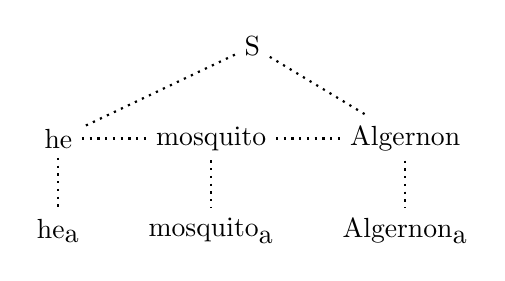
\begin{tikzpicture}[
    every node/.style={align=center},
    dotted line/.style={draw, dotted, thick},
    curved arrow/.style={draw, thick, -{Latex[bend]}},
    ]
\node (S) at (2.771330,0.000000) {S};
\node (he) at (0.307528,-1.171530) {he};
\node (mosquito) at (2.248532,-1.171530) {mosquito};
\node (Algernon) at (4.712334,-1.171530) {Algernon};
\draw[dotted line] (S) -- (he);
\draw[dotted line] (S) -- (Algernon);
\draw[dotted line] (he) -- (mosquito);
\draw[dotted line] (mosquito) -- (Algernon);
\node (heA) at (0.307528,-2.343060) {${\textrm{he}_{\textrm{a}}}$};
\node (mosquitoA) at (2.248532,-2.343060) {${\textrm{mosquito}_{\textrm{a}}}$};
\node (AlgernonA) at (4.712334,-2.343060) {${\textrm{Algernon}_{\textrm{a}}}$};
\draw[dotted line] (he) -- (heA);
\draw[dotted line] (mosquito) -- (mosquitoA);
\draw[dotted line] (Algernon) -- (AlgernonA);
\end{tikzpicture}
}
\end{minipage}
\bigbreak

\bigbreak
\begin{minipage}{\textwidth}
  \makebox[\textwidth][c]{
  \begin{tabular}{|l|l|l|}
    \hline
    \multicolumn{3}{|c|}{\textbf{Chaining}} \\
    \hline
    \textbf{\texttt{he}} & \textbf{\texttt{mosquito}}
    & \textbf{\texttt{Algernon}} \\
    ${\texttt{he}_{\texttt{a}}}$ & ${\texttt{mosquito}_{\texttt{a}}}$
    & ${\texttt{Algernon}_{\texttt{a}}}$ \\
    \hline
  \end{tabular}
  }
\end{minipage}
\bigbreak

\bigbreak
\begin{minipage}{\textwidth}
  \makebox[\textwidth][c]{
  \begin{tabular}{|c|}
    \hline
    \multicolumn{1}{|c|}{\textbf{Interpretations}} \\
    \hline
    NONE \\
    \hline
  \end{tabular}
  }
\end{minipage}
\bigbreak

\clearpage

%%%%%%%%%%%%%%%%%%%%%%%%%%%%%%%%%%%%%%%%%%%%%%%%%%%%%%%%%%%%%%%%
%
%     (1.91) After John Adams woke up, he was hungry.
%
%%%%%%%%%%%%%%%%%%%%%%%%%%%%%%%%%%%%%%%%%%%%%%%%%%%%%%%%%%%%%%%%

\section*{(1.91) After John Adams woke up, he was hungry.}
\addcontentsline{toc}{section}{(1.91) After John Adams woke up, he was hungry.}

\bigbreak
\begin{enumerate*}
\item[(1.91)] After John Adams woke up, he was hungry.
\end{enumerate*}
\bigbreak
\bigbreak
\begin{minipage}{\textwidth}
\makebox[\textwidth][c]{
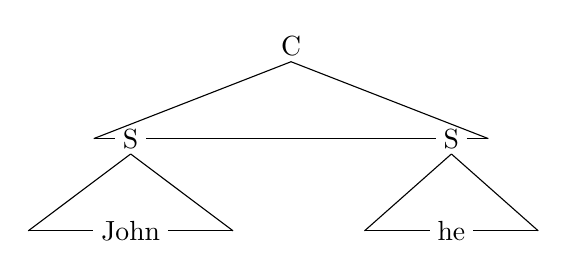
\begin{tikzpicture}
\node at (0.000000, 0.000000) {C};
\node at (-2.036768, -1.171530) {S};
\node at (-2.036768, -2.343060) {John};
\node at (2.036768, -1.171530) {S};
\node at (2.036768, -2.343060) {he};
\draw (0.000000,-0.195255) -- (-2.505383,-1.171530);
\draw (0.000000,-0.195255) -- (2.505383,-1.171530);
\draw (-2.505383,-1.171530) -- (-2.234396,-1.171530);
\draw (-1.839140,-1.171530) -- (1.839140,-1.171530);
\draw (2.234396,-1.171530) -- (2.505383,-1.171530);
\draw (-2.036768,-1.366785) -- (-3.337663,-2.343060);
\draw (-2.036768,-1.366785) -- (-0.735872,-2.343060);
\draw (-3.337663,-2.343060) -- (-2.510195,-2.343060);
\draw (-1.563340,-2.343060) -- (-0.735872,-2.343060);
\draw (2.036768,-1.366785) -- (0.933570,-2.343060);
\draw (2.036768,-1.366785) -- (3.139966,-2.343060);
\draw (0.933570,-2.343060) -- (1.761037,-2.343060);
\draw (2.312498,-2.343060) -- (3.139966,-2.343060);
\end{tikzpicture}
}
\end{minipage}
\bigbreak

\bigbreak
\begin{minipage}{\textwidth}
  \makebox[\textwidth][c]{
  \begin{tabular}{|r|c|c|c|c|c|c|c|c|c|}
    \hline
    \multicolumn{10}{|c|}{\textbf{Features}} \\
    \hline
    & \textbf{\texttt{PNF}}
    & \textbf{\texttt{FPF}} & \textbf{\texttt{SPF}}
    & \textbf{\texttt{TPF}} & \textbf{\texttt{PLF}}
    & \textbf{\texttt{GNF}} & \textbf{\texttt{ANF}}
    & \textbf{\texttt{RPF}} & \textbf{\texttt{GEN}} \\
    \textbf{\texttt{John}} & \texttt{-}
    & \texttt{-} & \texttt{-}
    & \texttt{+} & \texttt{-}
    & \texttt{-} & \texttt{+}
    & \texttt{-} & \texttt{-} \\
    \textbf{\texttt{he}} & \texttt{+}
    & \texttt{-} & \texttt{-}
    & \texttt{+} & \texttt{-}
    & \texttt{-} & \texttt{+}
    & \texttt{-} & \texttt{-} \\
    \hline
  \end{tabular}
  }
\end{minipage}
\bigbreak

\bigbreak
\begin{minipage}{\textwidth}
  \makebox[\textwidth][c]{
  \begin{tabular}{|r|l|}
    \hline
    \multicolumn{2}{|c|}{\textbf{Nodes}} \\
    \hline
    ${\textbf{\textrm{1}}_{\phantom{z}}}$ & \texttt{\texttt{(C,~up:0,~dn:2,~lt:0,~rt:0,~th:2,~nu:1)}} \\
    ${\textbf{\textrm{2}}_{\phantom{z}}}$ & \texttt{\texttt{(S,~up:1,~dn:3,~lt:0,~rt:4,~th:3,~nu:2)}} \\
    ${\textbf{\textrm{3}}_{\phantom{z}}}$ & \texttt{\texttt{(N,~lit:John,~ftr:[---+--+--],~up:2,~dn:0,}} \\
    & \texttt{\texttt{~lt:0,~rt:0,~th:4,~np:3,~ch:0,~co:${\textrm{3}_{\textrm{a}}}$,~ec:${\textrm{3}_{\textrm{b}}}$,}} \\
    & \texttt{\texttt{~pr:0,~su:5,~nu:3)}} \\
    ${\textbf{\textrm{3}}_{\textbf{\textrm{a}}}}$ & \texttt{\texttt{(E,~sub:A,~ftr:[---+--+--],~np:3,~ch:0,~co:${\textrm{3}_{\textrm{b}}}$)}} \\
    ${\textbf{\textrm{3}}_{\textbf{\textrm{b}}}}$ & \texttt{\texttt{(E,~sub:B,~ftr:[---+--+--],~np:3,~ch:${\textrm{5}_{\textrm{a}}}$,~co:0)}} \\
    ${\textbf{\textrm{4}}_{\phantom{z}}}$ & \texttt{\texttt{(S,~up:1,~dn:5,~lt:2,~rt:0,~th:5,~nu:4)}} \\
    ${\textbf{\textrm{5}}_{\phantom{z}}}$ & \texttt{\texttt{(N,~lit:he,~ftr:[+--+--+--],~up:4,~dn:0,}} \\
    & \texttt{\texttt{~lt:0,~rt:0,~th:0,~np:5,~ch:0,~co:${\textrm{5}_{\textrm{a}}}$,~ec:${\textrm{5}_{\textrm{a}}}$,}} \\
    & \texttt{\texttt{~pr:3,~su:0,~nu:5)}} \\
    ${\textbf{\textrm{5}}_{\textbf{\textrm{a}}}}$ & \texttt{\texttt{(E,~sub:A,~ftr:[+--+--+--],~np:5,~ch:0,~co:0)}} \\
    \hline
  \end{tabular}
  }
\end{minipage}
\bigbreak

\bigbreak
\begin{minipage}{\textwidth}
\makebox[\textwidth][c]{
\begin{tikzpicture}[
    every node/.style={align=center},
    dotted line/.style={draw, dotted, thick},
    curved arrow/.style={draw, thick, -{Latex[bend]}},
    ]
\node (S) at (1.214084,0.000000) {S};
\node (John) at (0.505225,-1.171530) {John};
\node (he) at (2.120639,-1.171530) {he};
\draw[dotted line] (S) -- (John);
\draw[dotted line] (S) -- (he);
\draw[dotted line] (John) -- (he);
\node (JohnA) at (0.505225,-2.343060) {${\textrm{John}_{\textrm{a}}}$};
\node (heA) at (2.120639,-2.343060) {${\textrm{he}_{\textrm{a}}}$};
\draw[dotted line] (John) -- (JohnA);
\draw[dotted line] (he) -- (heA);
\node (JohnB) at (0.505225,-3.514590) {${\textrm{John}_{\textrm{b}}}$};
\draw[dotted line] (JohnA) -- (JohnB);
\draw[curved arrow] (JohnB.north east) to [out=58.59,in=-121.41] (heA.south west);
\end{tikzpicture}
}
\end{minipage}
\bigbreak

\bigbreak
\begin{minipage}{\textwidth}
  \makebox[\textwidth][c]{
  \begin{tabular}{|l|l|}
    \hline
    \multicolumn{2}{|c|}{\textbf{Chaining}} \\
    \hline
    \textbf{\texttt{John}} & \textbf{\texttt{he}} \\
    ${\texttt{John}_{\texttt{a}}}$ & ${\texttt{he}_{\texttt{a}}}$ \\
    ${\texttt{John}_{\texttt{b}}}$\texttt{\symbol{94}}${\texttt{he}_{\texttt{a}}}$ &  \\
    \hline
  \end{tabular}
  }
\end{minipage}
\bigbreak

\bigbreak
\begin{minipage}{\textwidth}
  \makebox[\textwidth][c]{
  \begin{tabular}{|c|}
    \hline
    \multicolumn{1}{|c|}{\textbf{Interpretations}} \\
    \hline
    ${\texttt{John}_{\texttt{b}}}$\texttt{\symbol{94}}${\texttt{he}_{\texttt{a}}}$ \\
    \hline
  \end{tabular}
  }
\end{minipage}
\bigbreak

\clearpage

%%%%%%%%%%%%%%%%%%%%%%%%%%%%%%%%%%%%%%%%%%%%%%%%%%%%%%%%%%%%%%%%
%
%     (1.92) That Oscar was unpopular didn't disturb him.
%
%%%%%%%%%%%%%%%%%%%%%%%%%%%%%%%%%%%%%%%%%%%%%%%%%%%%%%%%%%%%%%%%

\section*{(1.92) That Oscar was unpopular didn't disturb him.}
\addcontentsline{toc}{section}{(1.92) That Oscar was unpopular didn't disturb him.}

\bigbreak
\begin{enumerate*}
\item[(1.92)] That Oscar was unpopular didn't disturb him.
\end{enumerate*}
\bigbreak
\bigbreak
\begin{minipage}{\textwidth}
\makebox[\textwidth][c]{
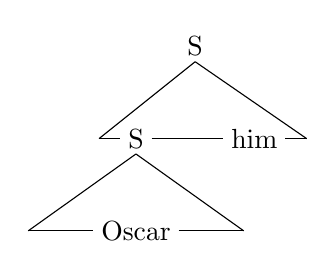
\begin{tikzpicture}
\node at (0.000000, 0.000000) {S};
\node at (-0.751737, -1.171530) {S};
\node at (-0.751737, -2.343060) {Oscar};
\node at (0.751737, -1.171530) {him};
\draw (0.000000,-0.195255) -- (-1.220352,-1.171530);
\draw (0.000000,-0.195255) -- (1.415608,-1.171530);
\draw (-1.220352,-1.171530) -- (-0.949365,-1.171530);
\draw (-0.554109,-1.171530) -- (0.358853,-1.171530);
\draw (1.144621,-1.171530) -- (1.415608,-1.171530);
\draw (-0.751737,-1.366785) -- (-2.119995,-2.343060);
\draw (-0.751737,-1.366785) -- (0.616521,-2.343060);
\draw (-2.119995,-2.343060) -- (-1.292527,-2.343060);
\draw (-0.210947,-2.343060) -- (0.616521,-2.343060);
\end{tikzpicture}
}
\end{minipage}
\bigbreak

\bigbreak
\begin{minipage}{\textwidth}
  \makebox[\textwidth][c]{
  \begin{tabular}{|r|c|c|c|c|c|c|c|c|c|}
    \hline
    \multicolumn{10}{|c|}{\textbf{Features}} \\
    \hline
    & \textbf{\texttt{PNF}}
    & \textbf{\texttt{FPF}} & \textbf{\texttt{SPF}}
    & \textbf{\texttt{TPF}} & \textbf{\texttt{PLF}}
    & \textbf{\texttt{GNF}} & \textbf{\texttt{ANF}}
    & \textbf{\texttt{RPF}} & \textbf{\texttt{GEN}} \\
    \textbf{\texttt{Oscar}} & \texttt{-}
    & \texttt{-} & \texttt{-}
    & \texttt{+} & \texttt{-}
    & \texttt{-} & \texttt{+}
    & \texttt{-} & \texttt{-} \\
    \textbf{\texttt{him}} & \texttt{+}
    & \texttt{-} & \texttt{-}
    & \texttt{+} & \texttt{-}
    & \texttt{-} & \texttt{+}
    & \texttt{-} & \texttt{-} \\
    \hline
  \end{tabular}
  }
\end{minipage}
\bigbreak

\bigbreak
\begin{minipage}{\textwidth}
  \makebox[\textwidth][c]{
  \begin{tabular}{|r|l|}
    \hline
    \multicolumn{2}{|c|}{\textbf{Nodes}} \\
    \hline
    ${\textbf{\textrm{1}}_{\phantom{z}}}$ & \texttt{\texttt{(S,~up:0,~dn:2,~lt:0,~rt:0,~th:2,~nu:1)}} \\
    ${\textbf{\textrm{2}}_{\phantom{z}}}$ & \texttt{\texttt{(S,~up:1,~dn:3,~lt:0,~rt:4,~th:3,~nu:2)}} \\
    ${\textbf{\textrm{3}}_{\phantom{z}}}$ & \texttt{\texttt{(N,~lit:Oscar,~ftr:[---+--+--],~up:2,~dn:0,}} \\
    & \texttt{\texttt{~lt:0,~rt:0,~th:4,~np:3,~ch:0,~co:${\textrm{3}_{\textrm{a}}}$,~ec:${\textrm{3}_{\textrm{b}}}$,}} \\
    & \texttt{\texttt{~pr:0,~su:4,~nu:3)}} \\
    ${\textbf{\textrm{3}}_{\textbf{\textrm{a}}}}$ & \texttt{\texttt{(E,~sub:A,~ftr:[---+--+--],~np:3,~ch:0,~co:${\textrm{3}_{\textrm{b}}}$)}} \\
    ${\textbf{\textrm{3}}_{\textbf{\textrm{b}}}}$ & \texttt{\texttt{(E,~sub:B,~ftr:[---+--+--],~np:3,~ch:${\textrm{4}_{\textrm{a}}}$,~co:0)}} \\
    ${\textbf{\textrm{4}}_{\phantom{z}}}$ & \texttt{\texttt{(N,~lit:him,~ftr:[+--+--+--],~up:1,~dn:0,}} \\
    & \texttt{\texttt{~lt:2,~rt:0,~th:0,~np:4,~ch:0,~co:${\textrm{4}_{\textrm{a}}}$,~ec:${\textrm{4}_{\textrm{a}}}$,}} \\
    & \texttt{\texttt{~pr:3,~su:0,~nu:4)}} \\
    ${\textbf{\textrm{4}}_{\textbf{\textrm{a}}}}$ & \texttt{\texttt{(E,~sub:A,~ftr:[+--+--+--],~np:4,~ch:0,~co:0)}} \\
    \hline
  \end{tabular}
  }
\end{minipage}
\bigbreak

\bigbreak
\begin{minipage}{\textwidth}
\makebox[\textwidth][c]{
\begin{tikzpicture}[
    every node/.style={align=center},
    dotted line/.style={draw, dotted, thick},
    curved arrow/.style={draw, thick, -{Latex[bend]}},
    ]
\node (S) at (1.398601,0.000000) {S};
\node (Oscar) at (0.572588,-1.171530) {Oscar};
\node (him) at (2.372519,-1.171530) {him};
\draw[dotted line] (S) -- (Oscar);
\draw[dotted line] (S) -- (him);
\draw[dotted line] (Oscar) -- (him);
\node (OscarA) at (0.572588,-2.343060) {${\textrm{Oscar}_{\textrm{a}}}$};
\node (himA) at (2.372519,-2.343060) {${\textrm{him}_{\textrm{a}}}$};
\draw[dotted line] (Oscar) -- (OscarA);
\draw[dotted line] (him) -- (himA);
\node (OscarB) at (0.572588,-3.514590) {${\textrm{Oscar}_{\textrm{b}}}$};
\draw[dotted line] (OscarA) -- (OscarB);
\draw[curved arrow] (OscarB.north east) to [out=58.59,in=-121.41] (himA.south west);
\end{tikzpicture}
}
\end{minipage}
\bigbreak

\bigbreak
\begin{minipage}{\textwidth}
  \makebox[\textwidth][c]{
  \begin{tabular}{|l|l|}
    \hline
    \multicolumn{2}{|c|}{\textbf{Chaining}} \\
    \hline
    \textbf{\texttt{Oscar}} & \textbf{\texttt{him}} \\
    ${\texttt{Oscar}_{\texttt{a}}}$ & ${\texttt{him}_{\texttt{a}}}$ \\
    ${\texttt{Oscar}_{\texttt{b}}}$\texttt{\symbol{94}}${\texttt{him}_{\texttt{a}}}$ &  \\
    \hline
  \end{tabular}
  }
\end{minipage}
\bigbreak

\bigbreak
\begin{minipage}{\textwidth}
  \makebox[\textwidth][c]{
  \begin{tabular}{|c|}
    \hline
    \multicolumn{1}{|c|}{\textbf{Interpretations}} \\
    \hline
    ${\texttt{Oscar}_{\texttt{b}}}$\texttt{\symbol{94}}${\texttt{him}_{\texttt{a}}}$ \\
    \hline
  \end{tabular}
  }
\end{minipage}
\bigbreak

\clearpage

%%%%%%%%%%%%%%%%%%%%%%%%%%%%%%%%%%%%%%%%%%%%%%%%%%%%%%%%%%%%%%%%
%
%     (1.93) For your brother to refuse to pay taxes would get him into trouble.
%
%%%%%%%%%%%%%%%%%%%%%%%%%%%%%%%%%%%%%%%%%%%%%%%%%%%%%%%%%%%%%%%%

\section*{(1.93) For your brother to refuse to pay taxes would get him into trouble.}
\addcontentsline{toc}{section}{(1.93) For your brother to refuse to pay taxes would get him into trouble.}

\bigbreak
\begin{enumerate*}
\item[(1.93)] For your brother to refuse to pay taxes would get him into trouble.
\end{enumerate*}
\bigbreak
\bigbreak
\begin{minipage}{\textwidth}
\makebox[\textwidth][c]{
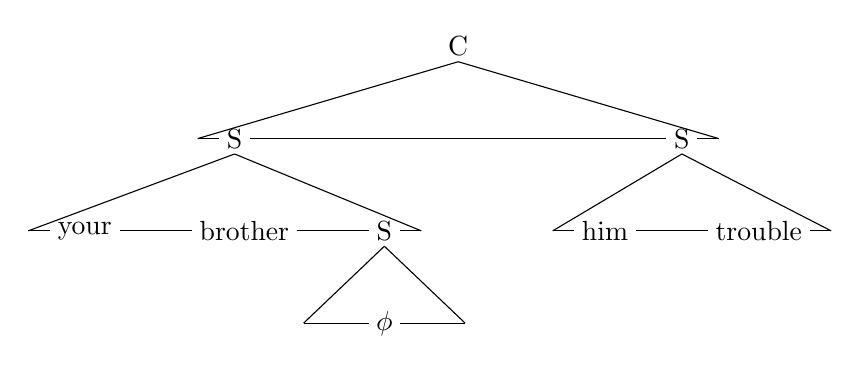
\begin{tikzpicture}
\node at (0.000000, 0.000000) {C};
\node at (-2.840491, -1.171530) {S};
\node at (-4.743019, -2.343060) {your};
\node at (-2.715771, -2.343060) {brother};
\node at (-0.937963, -2.343060) {S};
\node at (-0.937963, -3.514590) {$\phi$};
\node at (2.840491, -1.171530) {S};
\node at (1.863966, -2.343060) {him};
\node at (3.817016, -2.343060) {trouble};
\draw (0.000000,-0.195255) -- (-3.309106,-1.171530);
\draw (0.000000,-0.195255) -- (3.309106,-1.171530);
\draw (-3.309106,-1.171530) -- (-3.038119,-1.171530);
\draw (-2.642863,-1.171530) -- (2.642863,-1.171530);
\draw (3.038119,-1.171530) -- (3.309106,-1.171530);
\draw (-2.840491,-1.366785) -- (-5.461073,-2.343060);
\draw (-2.840491,-1.366785) -- (-0.469348,-2.343060);
\draw (-5.461073,-2.343060) -- (-5.190086,-2.343060);
\draw (-4.295951,-2.343060) -- (-3.382989,-2.343060);
\draw (-2.048552,-2.343060) -- (-1.135591,-2.343060);
\draw (-0.740335,-2.343060) -- (-0.469348,-2.343060);
\draw (-0.937963,-2.538315) -- (-1.963059,-3.514590);
\draw (-0.937963,-2.538315) -- (0.087133,-3.514590);
\draw (-1.963059,-3.514590) -- (-1.135591,-3.514590);
\draw (-0.740335,-3.514590) -- (0.087133,-3.514590);
\draw (2.840491,-1.366785) -- (1.200094,-2.343060);
\draw (2.840491,-1.366785) -- (4.735208,-2.343060);
\draw (1.200094,-2.343060) -- (1.471081,-2.343060);
\draw (2.256850,-2.343060) -- (3.169811,-2.343060);
\draw (4.464221,-2.343060) -- (4.735208,-2.343060);
\end{tikzpicture}
}
\end{minipage}
\bigbreak

\bigbreak
\begin{minipage}{\textwidth}
  \makebox[\textwidth][c]{
  \begin{tabular}{|r|c|c|c|c|c|c|c|c|c|}
    \hline
    \multicolumn{10}{|c|}{\textbf{Features}} \\
    \hline
    & \textbf{\texttt{PNF}}
    & \textbf{\texttt{FPF}} & \textbf{\texttt{SPF}}
    & \textbf{\texttt{TPF}} & \textbf{\texttt{PLF}}
    & \textbf{\texttt{GNF}} & \textbf{\texttt{ANF}}
    & \textbf{\texttt{RPF}} & \textbf{\texttt{GEN}} \\
    \textbf{\texttt{your}} & \texttt{+}
    & \texttt{-} & \texttt{+}
    & \texttt{-} & \texttt{?}
    & \texttt{?} & \texttt{+}
    & \texttt{-} & \texttt{+} \\
    \textbf{\texttt{brother}} & \texttt{-}
    & \texttt{-} & \texttt{-}
    & \texttt{+} & \texttt{-}
    & \texttt{-} & \texttt{+}
    & \texttt{-} & \texttt{-} \\
    $\bm{\phi}$ & \texttt{+}
    & \texttt{?} & \texttt{?}
    & \texttt{?} & \texttt{?}
    & \texttt{?} & \texttt{?}
    & \texttt{-} & \texttt{-} \\
    \textbf{\texttt{him}} & \texttt{+}
    & \texttt{-} & \texttt{-}
    & \texttt{+} & \texttt{-}
    & \texttt{-} & \texttt{+}
    & \texttt{-} & \texttt{-} \\
    \textbf{\texttt{trouble}} & \texttt{-}
    & \texttt{-} & \texttt{-}
    & \texttt{+} & \texttt{-}
    & \texttt{?} & \texttt{-}
    & \texttt{-} & \texttt{-} \\
    \hline
  \end{tabular}
  }
\end{minipage}
\bigbreak

\bigbreak
\begin{minipage}{\textwidth}
  \makebox[\textwidth][c]{
  \begin{tabular}{|r|l|}
    \hline
    \multicolumn{2}{|c|}{\textbf{Nodes}} \\
    \hline
    ${\textbf{\textrm{1}}_{\phantom{z}}}$ & \texttt{\texttt{(C,~up:0,~dn:2,~lt:0,~rt:0,~th:2,~nu:1)}} \\
    ${\textbf{\textrm{2}}_{\phantom{z}}}$ & \texttt{\texttt{(S,~up:1,~dn:3,~lt:0,~rt:7,~th:3,~nu:2)}} \\
    ${\textbf{\textrm{3}}_{\phantom{z}}}$ & \texttt{\texttt{(N,~lit:your,~ftr:[+-+-??+-+],~up:2,~dn:0,}} \\
    & \texttt{\texttt{~lt:0,~rt:4,~th:4,~np:3,~ch:0,~co:${\textrm{3}_{\textrm{a}}}$,~ec:${\textrm{3}_{\textrm{a}}}$,}} \\
    & \texttt{\texttt{~pr:0,~su:4,~nu:3)}} \\
    ${\textbf{\textrm{3}}_{\textbf{\textrm{a}}}}$ & \texttt{\texttt{(E,~sub:A,~ftr:[+-+-??+-+],~np:3,~ch:0,~co:0)}} \\
    ${\textbf{\textrm{4}}_{\phantom{z}}}$ & \texttt{\texttt{(N,~lit:brother,~ftr:[---+--+--],~up:2,~dn:0,}} \\
    & \texttt{\texttt{~lt:3,~rt:5,~th:5,~np:4,~ch:0,~co:${\textrm{4}_{\textrm{a}}}$,~ec:${\textrm{4}_{\textrm{d}}}$,}} \\
    & \texttt{\texttt{~pr:3,~su:6,~nu:4)}} \\
    ${\textbf{\textrm{4}}_{\textbf{\textrm{a}}}}$ & \texttt{\texttt{(E,~sub:A,~ftr:[---+--+--],~np:4,~ch:0,~co:${\textrm{4}_{\textrm{b}}}$)}} \\
    ${\textbf{\textrm{4}}_{\textbf{\textrm{b}}}}$ & \texttt{\texttt{(E,~sub:B,~ftr:[---+--+--],~np:4,~ch:${\textrm{8}_{\textrm{a}}}$,~co:${\textrm{4}_{\textrm{c}}}$)}} \\
    ${\textbf{\textrm{4}}_{\textbf{\textrm{c}}}}$ & \texttt{\texttt{(E,~sub:C,~ftr:[---+--+--],~np:4,~ch:${\textrm{6}_{\textrm{a}}}$,~co:${\textrm{4}_{\textrm{d}}}$)}} \\
    ${\textbf{\textrm{4}}_{\textbf{\textrm{d}}}}$ & \texttt{\texttt{(E,~sub:D,~ftr:[---+--+--],~np:4,~ch:${\textrm{6}_{\textrm{b}}}$,~co:0)}} \\
    ${\textbf{\textrm{5}}_{\phantom{z}}}$ & \texttt{\texttt{(S,~up:2,~dn:6,~lt:4,~rt:0,~th:6,~nu:5)}} \\
    ${\textbf{\textrm{6}}_{\phantom{z}}}$ & \texttt{\texttt{(N,~lit:$\phi$,~ftr:[+??????--],~up:5,~dn:0,}} \\
    & \texttt{\texttt{~lt:0,~rt:0,~th:7,~np:6,~ch:0,~co:${\textrm{6}_{\textrm{a}}}$,~ec:${\textrm{6}_{\textrm{b}}}$,}} \\
    & \texttt{\texttt{~pr:4,~su:8,~nu:6)}} \\
    ${\textbf{\textrm{6}}_{\textbf{\textrm{a}}}}$ & \texttt{\texttt{(E,~sub:A,~ftr:[+??????--],~np:6,~ch:0,~co:${\textrm{6}_{\textrm{b}}}$)}} \\
    ${\textbf{\textrm{6}}_{\textbf{\textrm{b}}}}$ & \texttt{\texttt{(E,~sub:B,~ftr:[+--+--+--],~np:6,~ch:${\textrm{8}_{\textrm{a}}}$,~co:0)}} \\
    ${\textbf{\textrm{7}}_{\phantom{z}}}$ & \texttt{\texttt{(S,~up:1,~dn:8,~lt:2,~rt:0,~th:8,~nu:7)}} \\
    ${\textbf{\textrm{8}}_{\phantom{z}}}$ & \texttt{\texttt{(N,~lit:him,~ftr:[+--+--+--],~up:7,~dn:0,}} \\
    & \texttt{\texttt{~lt:0,~rt:9,~th:9,~np:8,~ch:0,~co:${\textrm{8}_{\textrm{a}}}$,~ec:${\textrm{8}_{\textrm{a}}}$,}} \\
    & \texttt{\texttt{~pr:6,~su:9,~nu:8)}} \\
    ${\textbf{\textrm{8}}_{\textbf{\textrm{a}}}}$ & \texttt{\texttt{(E,~sub:A,~ftr:[+--+--+--],~np:8,~ch:0,~co:0)}} \\
    ${\textbf{\textrm{9}}_{\phantom{z}}}$ & \texttt{\texttt{(N,~lit:trouble,~ftr:[---+-?---],~up:7,~dn:0,}} \\
    & \texttt{\texttt{~lt:8,~rt:0,~th:0,~np:9,~ch:0,~co:${\textrm{9}_{\textrm{a}}}$,~ec:${\textrm{9}_{\textrm{a}}}$,}} \\
    & \texttt{\texttt{~pr:8,~su:0,~nu:9)}} \\
    ${\textbf{\textrm{9}}_{\textbf{\textrm{a}}}}$ & \texttt{\texttt{(E,~sub:A,~ftr:[---+-?---],~np:9,~ch:0,~co:0)}} \\
    \hline
  \end{tabular}
  }
\end{minipage}
\bigbreak

\bigbreak
\begin{minipage}{\textwidth}
\makebox[\textwidth][c]{
\begin{tikzpicture}[
    every node/.style={align=center},
    dotted line/.style={draw, dotted, thick},
    curved arrow/.style={draw, thick, -{Latex[bend]}},
    ]
\node (S) at (4.333537,0.000000) {S};
\node (your) at (0.478866,-1.171530) {your};
\node (brother) at (2.459409,-1.171530) {brother};
\node (PHI) at (4.407734,-1.171530) {$\phi$};
\node (him) at (6.081725,-1.171530) {him};
\node (trouble) at (7.988071,-1.171530) {trouble};
\draw[dotted line] (S) -- (your);
\draw[dotted line] (S) -- (trouble);
\draw[dotted line] (your) -- (brother);
\draw[dotted line] (brother) -- (PHI);
\draw[dotted line] (PHI) -- (him);
\draw[dotted line] (him) -- (trouble);
\node (yourA) at (0.478866,-2.343060) {${\textrm{your}_{\textrm{a}}}$};
\node (brotherA) at (2.459409,-2.343060) {${\textrm{brother}_{\textrm{a}}}$};
\node (PHIA) at (4.407734,-2.343060) {${\phi_{\textrm{a}}}$};
\node (himA) at (6.081725,-2.343060) {${\textrm{him}_{\textrm{a}}}$};
\node (troubleA) at (7.988071,-2.343060) {${\textrm{trouble}_{\textrm{a}}}$};
\draw[dotted line] (your) -- (yourA);
\draw[dotted line] (brother) -- (brotherA);
\draw[dotted line] (PHI) -- (PHIA);
\draw[dotted line] (him) -- (himA);
\draw[dotted line] (trouble) -- (troubleA);
\node (brotherB) at (2.459409,-3.514590) {${\textrm{brother}_{\textrm{b}}}$};
\node (PHIB) at (4.407734,-3.514590) {${\phi_{\textrm{b}}}$};
\draw[dotted line] (brotherA) -- (brotherB);
\draw[dotted line] (PHIA) -- (PHIB);
\node (brotherC) at (2.459409,-4.686120) {${\textrm{brother}_{\textrm{c}}}$};
\draw[dotted line] (brotherB) -- (brotherC);
\node (brotherD) at (2.459409,-5.857650) {${\textrm{brother}_{\textrm{d}}}$};
\draw[dotted line] (brotherC) -- (brotherD);
\draw[curved arrow] (PHIB.north east) to [out=58.59,in=-81.23] (himA.south);
\draw[curved arrow] (brotherB.north east) to [out=39.31,in=179.13] (himA.west);
\draw[curved arrow] (brotherC.north) to [out=73.02,in=-106.98] (PHIA.south);
\draw[curved arrow] (brotherD.north) to [out=73.02,in=-106.98] (PHIB.south);
\end{tikzpicture}
}
\end{minipage}
\bigbreak

\bigbreak
\begin{minipage}{\textwidth}
  \makebox[\textwidth][c]{
  \begin{tabular}{|l|l|l|l|l|}
    \hline
    \multicolumn{5}{|c|}{\textbf{Chaining}} \\
    \hline
    \textbf{\texttt{your}} & \textbf{\texttt{brother}}
    & $\bm{\phi}$ & \textbf{\texttt{him}}
    & \textbf{\texttt{trouble}} \\
    ${\texttt{your}_{\texttt{a}}}$ & ${\texttt{brother}_{\texttt{a}}}$
    & ${\phi_{\texttt{a}}}$ & ${\texttt{him}_{\texttt{a}}}$
    & ${\texttt{trouble}_{\texttt{a}}}$ \\
     & ${\texttt{brother}_{\texttt{b}}}$\texttt{\symbol{94}}${\texttt{him}_{\texttt{a}}}$
    & ${\phi_{\texttt{b}}}$\texttt{\symbol{94}}${\texttt{him}_{\texttt{a}}}$ & 
    &  \\
     & ${\texttt{brother}_{\texttt{c}}}$\texttt{\symbol{94}}${\phi_{\texttt{a}}}$
    &  & 
    &  \\
     & ${\texttt{brother}_{\texttt{d}}}$\texttt{\symbol{94}}${\phi_{\texttt{b}}}$
    &  & 
    &  \\
    \hline
  \end{tabular}
  }
\end{minipage}
\bigbreak

\bigbreak
\begin{minipage}{\textwidth}
  \makebox[\textwidth][c]{
  \begin{tabular}{|c|}
    \hline
    \multicolumn{1}{|c|}{\textbf{Interpretations}} \\
    \hline
    ${\texttt{brother}_{\texttt{d}}}$\texttt{\symbol{94}}${\phi_{\texttt{b}}}$\texttt{\symbol{94}}${\texttt{him}_{\texttt{a}}}$ \\
    \hline
  \end{tabular}
  }
\end{minipage}
\bigbreak

\clearpage

%%%%%%%%%%%%%%%%%%%%%%%%%%%%%%%%%%%%%%%%%%%%%%%%%%%%%%%%%%%%%%%%
%
%     (1.94) Anna's complaining about Peter infuriated him.
%
%%%%%%%%%%%%%%%%%%%%%%%%%%%%%%%%%%%%%%%%%%%%%%%%%%%%%%%%%%%%%%%%

\section*{(1.94) Anna's complaining about Peter infuriated him.}
\addcontentsline{toc}{section}{(1.94) Anna's complaining about Peter infuriated him.}

\bigbreak
\begin{enumerate*}
\item[(1.94)] Anna's complaining about Peter infuriated him.
\end{enumerate*}
\bigbreak
\bigbreak
\begin{minipage}{\textwidth}
\makebox[\textwidth][c]{
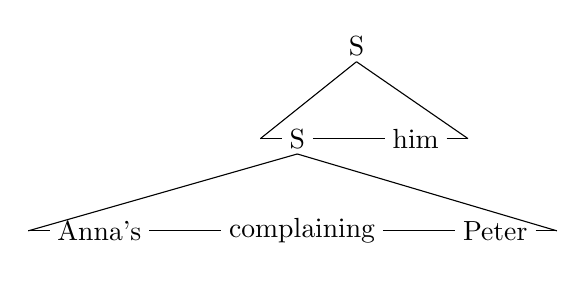
\begin{tikzpicture}
\node at (0.000000, 0.000000) {S};
\node at (-0.751737, -1.171530) {S};
\node at (-3.265172, -2.343060) {Anna's};
\node at (-0.691695, -2.343060) {complaining};
\node at (1.761699, -2.343060) {Peter};
\node at (0.751737, -1.171530) {him};
\draw (0.000000,-0.195255) -- (-1.220352,-1.171530);
\draw (0.000000,-0.195255) -- (1.415608,-1.171530);
\draw (-1.220352,-1.171530) -- (-0.949365,-1.171530);
\draw (-0.554109,-1.171530) -- (0.358853,-1.171530);
\draw (1.144621,-1.171530) -- (1.415608,-1.171530);
\draw (-0.751737,-1.366785) -- (-4.169208,-2.343060);
\draw (-0.751737,-1.366785) -- (2.545652,-2.343060);
\draw (-4.169208,-2.343060) -- (-3.898221,-2.343060);
\draw (-2.632123,-2.343060) -- (-1.719162,-2.343060);
\draw (0.335771,-2.343060) -- (1.248733,-2.343060);
\draw (2.274665,-2.343060) -- (2.545652,-2.343060);
\end{tikzpicture}
}
\end{minipage}
\bigbreak

\bigbreak
\begin{minipage}{\textwidth}
  \makebox[\textwidth][c]{
  \begin{tabular}{|r|c|c|c|c|c|c|c|c|c|}
    \hline
    \multicolumn{10}{|c|}{\textbf{Features}} \\
    \hline
    & \textbf{\texttt{PNF}}
    & \textbf{\texttt{FPF}} & \textbf{\texttt{SPF}}
    & \textbf{\texttt{TPF}} & \textbf{\texttt{PLF}}
    & \textbf{\texttt{GNF}} & \textbf{\texttt{ANF}}
    & \textbf{\texttt{RPF}} & \textbf{\texttt{GEN}} \\
    \textbf{\texttt{Anna's}} & \texttt{-}
    & \texttt{-} & \texttt{-}
    & \texttt{+} & \texttt{-}
    & \texttt{+} & \texttt{+}
    & \texttt{-} & \texttt{+} \\
    \textbf{\texttt{complaining}} & \texttt{-}
    & \texttt{-} & \texttt{-}
    & \texttt{+} & \texttt{-}
    & \texttt{?} & \texttt{-}
    & \texttt{-} & \texttt{-} \\
    \textbf{\texttt{Peter}} & \texttt{-}
    & \texttt{-} & \texttt{-}
    & \texttt{+} & \texttt{-}
    & \texttt{-} & \texttt{+}
    & \texttt{-} & \texttt{-} \\
    \textbf{\texttt{him}} & \texttt{+}
    & \texttt{-} & \texttt{-}
    & \texttt{+} & \texttt{-}
    & \texttt{-} & \texttt{+}
    & \texttt{-} & \texttt{-} \\
    \hline
  \end{tabular}
  }
\end{minipage}
\bigbreak

\bigbreak
\begin{minipage}{\textwidth}
  \makebox[\textwidth][c]{
  \begin{tabular}{|r|l|}
    \hline
    \multicolumn{2}{|c|}{\textbf{Nodes}} \\
    \hline
    ${\textbf{\textrm{1}}_{\phantom{z}}}$ & \texttt{\texttt{(S,~up:0,~dn:2,~lt:0,~rt:0,~th:2,~nu:1)}} \\
    ${\textbf{\textrm{2}}_{\phantom{z}}}$ & \texttt{\texttt{(S,~up:1,~dn:3,~lt:0,~rt:6,~th:3,~nu:2)}} \\
    ${\textbf{\textrm{3}}_{\phantom{z}}}$ & \texttt{\texttt{(N,~lit:Anna's,~ftr:[---+-++-+],~up:2,~dn:0,}} \\
    & \texttt{\texttt{~lt:0,~rt:4,~th:4,~np:3,~ch:0,~co:${\textrm{3}_{\textrm{a}}}$,~ec:${\textrm{3}_{\textrm{a}}}$,}} \\
    & \texttt{\texttt{~pr:0,~su:4,~nu:3)}} \\
    ${\textbf{\textrm{3}}_{\textbf{\textrm{a}}}}$ & \texttt{\texttt{(E,~sub:A,~ftr:[---+-++-+],~np:3,~ch:0,~co:0)}} \\
    ${\textbf{\textrm{4}}_{\phantom{z}}}$ & \texttt{\texttt{(N,~lit:complaining,~ftr:[---+-?---],~up:2,~dn:0,}} \\
    & \texttt{\texttt{~lt:3,~rt:5,~th:5,~np:4,~ch:0,~co:${\textrm{4}_{\textrm{a}}}$,~ec:${\textrm{4}_{\textrm{a}}}$,}} \\
    & \texttt{\texttt{~pr:3,~su:5,~nu:4)}} \\
    ${\textbf{\textrm{4}}_{\textbf{\textrm{a}}}}$ & \texttt{\texttt{(E,~sub:A,~ftr:[---+-?---],~np:4,~ch:0,~co:0)}} \\
    ${\textbf{\textrm{5}}_{\phantom{z}}}$ & \texttt{\texttt{(N,~lit:Peter,~ftr:[---+--+--],~up:2,~dn:0,}} \\
    & \texttt{\texttt{~lt:4,~rt:0,~th:6,~np:5,~ch:0,~co:${\textrm{5}_{\textrm{a}}}$,~ec:${\textrm{5}_{\textrm{b}}}$,}} \\
    & \texttt{\texttt{~pr:4,~su:6,~nu:5)}} \\
    ${\textbf{\textrm{5}}_{\textbf{\textrm{a}}}}$ & \texttt{\texttt{(E,~sub:A,~ftr:[---+--+--],~np:5,~ch:0,~co:${\textrm{5}_{\textrm{b}}}$)}} \\
    ${\textbf{\textrm{5}}_{\textbf{\textrm{b}}}}$ & \texttt{\texttt{(E,~sub:B,~ftr:[---+--+--],~np:5,~ch:${\textrm{6}_{\textrm{a}}}$,~co:0)}} \\
    ${\textbf{\textrm{6}}_{\phantom{z}}}$ & \texttt{\texttt{(N,~lit:him,~ftr:[+--+--+--],~up:1,~dn:0,}} \\
    & \texttt{\texttt{~lt:2,~rt:0,~th:0,~np:6,~ch:0,~co:${\textrm{6}_{\textrm{a}}}$,~ec:${\textrm{6}_{\textrm{a}}}$,}} \\
    & \texttt{\texttt{~pr:5,~su:0,~nu:6)}} \\
    ${\textbf{\textrm{6}}_{\textbf{\textrm{a}}}}$ & \texttt{\texttt{(E,~sub:A,~ftr:[+--+--+--],~np:6,~ch:0,~co:0)}} \\
    \hline
  \end{tabular}
  }
\end{minipage}
\bigbreak

\bigbreak
\begin{minipage}{\textwidth}
\makebox[\textwidth][c]{
\begin{tikzpicture}[
    every node/.style={align=center},
    dotted line/.style={draw, dotted, thick},
    curved arrow/.style={draw, thick, -{Latex[bend]}},
    ]
\node (S) at (3.897549,0.000000) {S};
\node (Anna's) at (0.664847,-1.171530) {Anna's};
\node (complaining) at (3.191619,-1.171530) {complaining};
\node (Peter) at (5.598309,-1.171530) {Peter};
\node (him) at (7.370415,-1.171530) {him};
\draw[dotted line] (S) -- (Anna's);
\draw[dotted line] (S) -- (him);
\draw[dotted line] (Anna's) -- (complaining);
\draw[dotted line] (complaining) -- (Peter);
\draw[dotted line] (Peter) -- (him);
\node (Anna'sA) at (0.664847,-2.343060) {${\textrm{Anna's}_{\textrm{a}}}$};
\node (complainingA) at (3.191619,-2.343060) {${\textrm{complaining}_{\textrm{a}}}$};
\node (PeterA) at (5.598309,-2.343060) {${\textrm{Peter}_{\textrm{a}}}$};
\node (himA) at (7.370415,-2.343060) {${\textrm{him}_{\textrm{a}}}$};
\draw[dotted line] (Anna's) -- (Anna'sA);
\draw[dotted line] (complaining) -- (complainingA);
\draw[dotted line] (Peter) -- (PeterA);
\draw[dotted line] (him) -- (himA);
\node (PeterB) at (5.598309,-3.514590) {${\textrm{Peter}_{\textrm{b}}}$};
\draw[dotted line] (PeterA) -- (PeterB);
\draw[curved arrow] (PeterB.north east) to [out=58.59,in=-121.41] (himA.south west);
\end{tikzpicture}
}
\end{minipage}
\bigbreak

\bigbreak
\begin{minipage}{\textwidth}
  \makebox[\textwidth][c]{
  \begin{tabular}{|l|l|l|l|}
    \hline
    \multicolumn{4}{|c|}{\textbf{Chaining}} \\
    \hline
    \textbf{\texttt{Anna's}} & \textbf{\texttt{complaining}}
    & \textbf{\texttt{Peter}} & \textbf{\texttt{him}} \\
    ${\texttt{Anna's}_{\texttt{a}}}$ & ${\texttt{complaining}_{\texttt{a}}}$
    & ${\texttt{Peter}_{\texttt{a}}}$ & ${\texttt{him}_{\texttt{a}}}$ \\
     & 
    & ${\texttt{Peter}_{\texttt{b}}}$\texttt{\symbol{94}}${\texttt{him}_{\texttt{a}}}$ &  \\
    \hline
  \end{tabular}
  }
\end{minipage}
\bigbreak

\bigbreak
\begin{minipage}{\textwidth}
  \makebox[\textwidth][c]{
  \begin{tabular}{|c|}
    \hline
    \multicolumn{1}{|c|}{\textbf{Interpretations}} \\
    \hline
    ${\texttt{Peter}_{\texttt{b}}}$\texttt{\symbol{94}}${\texttt{him}_{\texttt{a}}}$ \\
    \hline
  \end{tabular}
  }
\end{minipage}
\bigbreak

\clearpage

%%%%%%%%%%%%%%%%%%%%%%%%%%%%%%%%%%%%%%%%%%%%%%%%%%%%%%%%%%%%%%%%
%
%     (1.95) The possibility that Fred will be unpopular doesn’t bother him.
%
%%%%%%%%%%%%%%%%%%%%%%%%%%%%%%%%%%%%%%%%%%%%%%%%%%%%%%%%%%%%%%%%

\section*{(1.95) The possibility that Fred will be unpopular doesn’t bother him.}
\addcontentsline{toc}{section}{(1.95) The possibility that Fred will be unpopular doesn’t bother him.}

\bigbreak
\begin{enumerate*}
\item[(1.95)] The possibility that Fred will be unpopular doesn’t bother him.
\end{enumerate*}
\bigbreak
\bigbreak
\begin{minipage}{\textwidth}
\makebox[\textwidth][c]{
\begin{tikzpicture}
\node at (0.000000, 0.000000) {S};
\node at (-1.746079, -1.171530) {possibility};
\node at (0.242606, -1.171530) {S};
\node at (0.242606, -2.343060) {Fred};
\node at (1.746079, -1.171530) {him};
\draw (0.000000,-0.195255) -- (-2.895162,-1.171530);
\draw (0.000000,-0.195255) -- (2.409951,-1.171530);
\draw (-2.895162,-1.171530) -- (-2.624175,-1.171530);
\draw (-0.867984,-1.171530) -- (0.044978,-1.171530);
\draw (0.440234,-1.171530) -- (1.353195,-1.171530);
\draw (2.138964,-1.171530) -- (2.409951,-1.171530);
\draw (0.242606,-1.366785) -- (-1.044133,-2.343060);
\draw (0.242606,-1.366785) -- (1.529344,-2.343060);
\draw (-1.044133,-2.343060) -- (-0.216665,-2.343060);
\draw (0.701876,-2.343060) -- (1.529344,-2.343060);
\end{tikzpicture}
}
\end{minipage}
\bigbreak

\bigbreak
\begin{minipage}{\textwidth}
  \makebox[\textwidth][c]{
  \begin{tabular}{|r|c|c|c|c|c|c|c|c|c|}
    \hline
    \multicolumn{10}{|c|}{\textbf{Features}} \\
    \hline
    & \textbf{\texttt{PNF}}
    & \textbf{\texttt{FPF}} & \textbf{\texttt{SPF}}
    & \textbf{\texttt{TPF}} & \textbf{\texttt{PLF}}
    & \textbf{\texttt{GNF}} & \textbf{\texttt{ANF}}
    & \textbf{\texttt{RPF}} & \textbf{\texttt{GEN}} \\
    \textbf{\texttt{possibility}} & \texttt{-}
    & \texttt{-} & \texttt{-}
    & \texttt{+} & \texttt{-}
    & \texttt{?} & \texttt{-}
    & \texttt{-} & \texttt{-} \\
    \textbf{\texttt{Fred}} & \texttt{-}
    & \texttt{-} & \texttt{-}
    & \texttt{+} & \texttt{-}
    & \texttt{-} & \texttt{+}
    & \texttt{-} & \texttt{-} \\
    \textbf{\texttt{him}} & \texttt{+}
    & \texttt{-} & \texttt{-}
    & \texttt{+} & \texttt{-}
    & \texttt{-} & \texttt{+}
    & \texttt{-} & \texttt{-} \\
    \hline
  \end{tabular}
  }
\end{minipage}
\bigbreak

\bigbreak
\begin{minipage}{\textwidth}
  \makebox[\textwidth][c]{
  \begin{tabular}{|r|l|}
    \hline
    \multicolumn{2}{|c|}{\textbf{Nodes}} \\
    \hline
    ${\textbf{\textrm{1}}_{\phantom{z}}}$ & \texttt{\texttt{(S,~up:0,~dn:2,~lt:0,~rt:0,~th:2,~nu:1)}} \\
    ${\textbf{\textrm{2}}_{\phantom{z}}}$ & \texttt{\texttt{(N,~lit:possibility,~ftr:[---+-?---],~up:1,~dn:0,}} \\
    & \texttt{\texttt{~lt:0,~rt:3,~th:3,~np:2,~ch:0,~co:${\textrm{2}_{\textrm{a}}}$,~ec:${\textrm{2}_{\textrm{a}}}$,}} \\
    & \texttt{\texttt{~pr:0,~su:4,~nu:2)}} \\
    ${\textbf{\textrm{2}}_{\textbf{\textrm{a}}}}$ & \texttt{\texttt{(E,~sub:A,~ftr:[---+-?---],~np:2,~ch:0,~co:0)}} \\
    ${\textbf{\textrm{3}}_{\phantom{z}}}$ & \texttt{\texttt{(S,~up:1,~dn:4,~lt:2,~rt:5,~th:4,~nu:3)}} \\
    ${\textbf{\textrm{4}}_{\phantom{z}}}$ & \texttt{\texttt{(N,~lit:Fred,~ftr:[---+--+--],~up:3,~dn:0,}} \\
    & \texttt{\texttt{~lt:0,~rt:0,~th:5,~np:4,~ch:0,~co:${\textrm{4}_{\textrm{a}}}$,~ec:${\textrm{4}_{\textrm{b}}}$,}} \\
    & \texttt{\texttt{~pr:2,~su:5,~nu:4)}} \\
    ${\textbf{\textrm{4}}_{\textbf{\textrm{a}}}}$ & \texttt{\texttt{(E,~sub:A,~ftr:[---+--+--],~np:4,~ch:0,~co:${\textrm{4}_{\textrm{b}}}$)}} \\
    ${\textbf{\textrm{4}}_{\textbf{\textrm{b}}}}$ & \texttt{\texttt{(E,~sub:B,~ftr:[---+--+--],~np:4,~ch:${\textrm{5}_{\textrm{a}}}$,~co:0)}} \\
    ${\textbf{\textrm{5}}_{\phantom{z}}}$ & \texttt{\texttt{(N,~lit:him,~ftr:[+--+--+--],~up:1,~dn:0,}} \\
    & \texttt{\texttt{~lt:3,~rt:0,~th:0,~np:5,~ch:0,~co:${\textrm{5}_{\textrm{a}}}$,~ec:${\textrm{5}_{\textrm{a}}}$,}} \\
    & \texttt{\texttt{~pr:4,~su:0,~nu:5)}} \\
    ${\textbf{\textrm{5}}_{\textbf{\textrm{a}}}}$ & \texttt{\texttt{(E,~sub:A,~ftr:[+--+--+--],~np:5,~ch:0,~co:0)}} \\
    \hline
  \end{tabular}
  }
\end{minipage}
\bigbreak

\bigbreak
\begin{minipage}{\textwidth}
\makebox[\textwidth][c]{
\begin{tikzpicture}[
    every node/.style={align=center},
    dotted line/.style={draw, dotted, thick},
    curved arrow/.style={draw, thick, -{Latex[bend]}},
    ]
\node (S) at (2.628305,0.000000) {S};
\node (possibility) at (0.909893,-1.171530) {possibility};
\node (Fred) at (3.113516,-1.171530) {Fred};
\node (him) at (4.831928,-1.171530) {him};
\draw[dotted line] (S) -- (possibility);
\draw[dotted line] (S) -- (him);
\draw[dotted line] (possibility) -- (Fred);
\draw[dotted line] (Fred) -- (him);
\node (possibilityA) at (0.909893,-2.343060) {${\textrm{possibility}_{\textrm{a}}}$};
\node (FredA) at (3.113516,-2.343060) {${\textrm{Fred}_{\textrm{a}}}$};
\node (himA) at (4.831928,-2.343060) {${\textrm{him}_{\textrm{a}}}$};
\draw[dotted line] (possibility) -- (possibilityA);
\draw[dotted line] (Fred) -- (FredA);
\draw[dotted line] (him) -- (himA);
\node (FredB) at (3.113516,-3.514590) {${\textrm{Fred}_{\textrm{b}}}$};
\draw[dotted line] (FredA) -- (FredB);
\draw[curved arrow] (FredB.north east) to [out=58.59,in=-121.41] (himA.south west);
\end{tikzpicture}
}
\end{minipage}
\bigbreak

\bigbreak
\begin{minipage}{\textwidth}
  \makebox[\textwidth][c]{
  \begin{tabular}{|l|l|l|}
    \hline
    \multicolumn{3}{|c|}{\textbf{Chaining}} \\
    \hline
    \textbf{\texttt{possibility}} & \textbf{\texttt{Fred}}
    & \textbf{\texttt{him}} \\
    ${\texttt{possibility}_{\texttt{a}}}$ & ${\texttt{Fred}_{\texttt{a}}}$
    & ${\texttt{him}_{\texttt{a}}}$ \\
     & ${\texttt{Fred}_{\texttt{b}}}$\texttt{\symbol{94}}${\texttt{him}_{\texttt{a}}}$
    &  \\
    \hline
  \end{tabular}
  }
\end{minipage}
\bigbreak

\bigbreak
\begin{minipage}{\textwidth}
  \makebox[\textwidth][c]{
  \begin{tabular}{|c|}
    \hline
    \multicolumn{1}{|c|}{\textbf{Interpretations}} \\
    \hline
    ${\texttt{Fred}_{\texttt{b}}}$\texttt{\symbol{94}}${\texttt{him}_{\texttt{a}}}$ \\
    \hline
  \end{tabular}
  }
\end{minipage}
\bigbreak

\clearpage

%%%%%%%%%%%%%%%%%%%%%%%%%%%%%%%%%%%%%%%%%%%%%%%%%%%%%%%%%%%%%%%%
%
%     (1.96) After he woke up, John Adams was hungry.
%
%%%%%%%%%%%%%%%%%%%%%%%%%%%%%%%%%%%%%%%%%%%%%%%%%%%%%%%%%%%%%%%%

\section*{(1.96) After he woke up, John Adams was hungry.}
\addcontentsline{toc}{section}{(1.96) After he woke up, John Adams was hungry.}

\bigbreak
\begin{enumerate*}
\item[(1.96)] After he woke up, John Adams was hungry.
\end{enumerate*}
\bigbreak
\bigbreak
\begin{minipage}{\textwidth}
\makebox[\textwidth][c]{
\begin{tikzpicture}
\node at (0.000000, 0.000000) {C};
\node at (-2.036768, -1.171530) {S};
\node at (-2.036768, -2.343060) {he};
\node at (2.036768, -1.171530) {S};
\node at (2.036768, -2.343060) {John};
\draw (0.000000,-0.195255) -- (-2.505383,-1.171530);
\draw (0.000000,-0.195255) -- (2.505383,-1.171530);
\draw (-2.505383,-1.171530) -- (-2.234396,-1.171530);
\draw (-1.839140,-1.171530) -- (1.839140,-1.171530);
\draw (2.234396,-1.171530) -- (2.505383,-1.171530);
\draw (-2.036768,-1.366785) -- (-3.139966,-2.343060);
\draw (-2.036768,-1.366785) -- (-0.933570,-2.343060);
\draw (-3.139966,-2.343060) -- (-2.312498,-2.343060);
\draw (-1.761037,-2.343060) -- (-0.933570,-2.343060);
\draw (2.036768,-1.366785) -- (0.735872,-2.343060);
\draw (2.036768,-1.366785) -- (3.337663,-2.343060);
\draw (0.735872,-2.343060) -- (1.563340,-2.343060);
\draw (2.510195,-2.343060) -- (3.337663,-2.343060);
\end{tikzpicture}
}
\end{minipage}
\bigbreak

\bigbreak
\begin{minipage}{\textwidth}
  \makebox[\textwidth][c]{
  \begin{tabular}{|r|c|c|c|c|c|c|c|c|c|}
    \hline
    \multicolumn{10}{|c|}{\textbf{Features}} \\
    \hline
    & \textbf{\texttt{PNF}}
    & \textbf{\texttt{FPF}} & \textbf{\texttt{SPF}}
    & \textbf{\texttt{TPF}} & \textbf{\texttt{PLF}}
    & \textbf{\texttt{GNF}} & \textbf{\texttt{ANF}}
    & \textbf{\texttt{RPF}} & \textbf{\texttt{GEN}} \\
    \textbf{\texttt{he}} & \texttt{+}
    & \texttt{-} & \texttt{-}
    & \texttt{+} & \texttt{-}
    & \texttt{-} & \texttt{+}
    & \texttt{-} & \texttt{-} \\
    \textbf{\texttt{John}} & \texttt{-}
    & \texttt{-} & \texttt{-}
    & \texttt{+} & \texttt{-}
    & \texttt{-} & \texttt{+}
    & \texttt{-} & \texttt{-} \\
    \hline
  \end{tabular}
  }
\end{minipage}
\bigbreak

\bigbreak
\begin{minipage}{\textwidth}
  \makebox[\textwidth][c]{
  \begin{tabular}{|r|l|}
    \hline
    \multicolumn{2}{|c|}{\textbf{Nodes}} \\
    \hline
    ${\textbf{\textrm{1}}_{\phantom{z}}}$ & \texttt{\texttt{(C,~up:0,~dn:2,~lt:0,~rt:0,~th:2,~nu:1)}} \\
    ${\textbf{\textrm{2}}_{\phantom{z}}}$ & \texttt{\texttt{(S,~up:1,~dn:3,~lt:0,~rt:4,~th:3,~nu:2)}} \\
    ${\textbf{\textrm{3}}_{\phantom{z}}}$ & \texttt{\texttt{(N,~lit:he,~ftr:[+--+--+--],~up:2,~dn:0,}} \\
    & \texttt{\texttt{~lt:0,~rt:0,~th:4,~np:3,~ch:0,~co:${\textrm{3}_{\textrm{a}}}$,~ec:${\textrm{3}_{\textrm{a}}}$,}} \\
    & \texttt{\texttt{~pr:0,~su:5,~nu:3)}} \\
    ${\textbf{\textrm{3}}_{\textbf{\textrm{a}}}}$ & \texttt{\texttt{(E,~sub:A,~ftr:[+--+--+--],~np:3,~ch:0,~co:0)}} \\
    ${\textbf{\textrm{4}}_{\phantom{z}}}$ & \texttt{\texttt{(S,~up:1,~dn:5,~lt:2,~rt:0,~th:5,~nu:4)}} \\
    ${\textbf{\textrm{5}}_{\phantom{z}}}$ & \texttt{\texttt{(N,~lit:John,~ftr:[---+--+--],~up:4,~dn:0,}} \\
    & \texttt{\texttt{~lt:0,~rt:0,~th:0,~np:5,~ch:0,~co:${\textrm{5}_{\textrm{a}}}$,~ec:${\textrm{5}_{\textrm{a}}}$,}} \\
    & \texttt{\texttt{~pr:3,~su:0,~nu:5)}} \\
    ${\textbf{\textrm{5}}_{\textbf{\textrm{a}}}}$ & \texttt{\texttt{(E,~sub:A,~ftr:[---+--+--],~np:5,~ch:0,~co:0)}} \\
    \hline
  \end{tabular}
  }
\end{minipage}
\bigbreak

\bigbreak
\begin{minipage}{\textwidth}
\makebox[\textwidth][c]{
\begin{tikzpicture}[
    every node/.style={align=center},
    dotted line/.style={draw, dotted, thick},
    curved arrow/.style={draw, thick, -{Latex[bend]}},
    ]
\node (S) at (1.214084,0.000000) {S};
\node (he) at (0.307528,-1.171530) {he};
\node (John) at (1.922942,-1.171530) {John};
\draw[dotted line] (S) -- (he);
\draw[dotted line] (S) -- (John);
\draw[dotted line] (he) -- (John);
\node (heA) at (0.307528,-2.343060) {${\textrm{he}_{\textrm{a}}}$};
\node (JohnA) at (1.922942,-2.343060) {${\textrm{John}_{\textrm{a}}}$};
\draw[dotted line] (he) -- (heA);
\draw[dotted line] (John) -- (JohnA);
\end{tikzpicture}
}
\end{minipage}
\bigbreak

\bigbreak
\begin{minipage}{\textwidth}
  \makebox[\textwidth][c]{
  \begin{tabular}{|l|l|}
    \hline
    \multicolumn{2}{|c|}{\textbf{Chaining}} \\
    \hline
    \textbf{\texttt{he}} & \textbf{\texttt{John}} \\
    ${\texttt{he}_{\texttt{a}}}$ & ${\texttt{John}_{\texttt{a}}}$ \\
    \hline
  \end{tabular}
  }
\end{minipage}
\bigbreak

\bigbreak
\begin{minipage}{\textwidth}
  \makebox[\textwidth][c]{
  \begin{tabular}{|c|}
    \hline
    \multicolumn{1}{|c|}{\textbf{Interpretations}} \\
    \hline
    NONE \\
    \hline
  \end{tabular}
  }
\end{minipage}
\bigbreak

\clearpage

%%%%%%%%%%%%%%%%%%%%%%%%%%%%%%%%%%%%%%%%%%%%%%%%%%%%%%%%%%%%%%%%
%
%     (1.97) That he was unpopular didn't disturb Oscar.
%
%%%%%%%%%%%%%%%%%%%%%%%%%%%%%%%%%%%%%%%%%%%%%%%%%%%%%%%%%%%%%%%%

\section*{(1.97) That he was unpopular didn't disturb Oscar.}
\addcontentsline{toc}{section}{(1.97) That he was unpopular didn't disturb Oscar.}

\bigbreak
\begin{enumerate*}
\item[(1.97)] That he was unpopular didn't disturb Oscar.
\end{enumerate*}
\bigbreak
\bigbreak
\begin{minipage}{\textwidth}
\makebox[\textwidth][c]{
\begin{tikzpicture}
\node at (0.000000, 0.000000) {S};
\node at (-0.825690, -1.171530) {S};
\node at (-0.825690, -2.343060) {he};
\node at (0.825690, -1.171530) {Oscar};
\draw (0.000000,-0.195255) -- (-1.294305,-1.171530);
\draw (0.000000,-0.195255) -- (1.637467,-1.171530);
\draw (-1.294305,-1.171530) -- (-1.023318,-1.171530);
\draw (-0.628062,-1.171530) -- (0.284900,-1.171530);
\draw (1.366480,-1.171530) -- (1.637467,-1.171530);
\draw (-0.825690,-1.366785) -- (-1.928888,-2.343060);
\draw (-0.825690,-1.366785) -- (0.277508,-2.343060);
\draw (-1.928888,-2.343060) -- (-1.101420,-2.343060);
\draw (-0.549960,-2.343060) -- (0.277508,-2.343060);
\end{tikzpicture}
}
\end{minipage}
\bigbreak

\bigbreak
\begin{minipage}{\textwidth}
  \makebox[\textwidth][c]{
  \begin{tabular}{|r|c|c|c|c|c|c|c|c|c|}
    \hline
    \multicolumn{10}{|c|}{\textbf{Features}} \\
    \hline
    & \textbf{\texttt{PNF}}
    & \textbf{\texttt{FPF}} & \textbf{\texttt{SPF}}
    & \textbf{\texttt{TPF}} & \textbf{\texttt{PLF}}
    & \textbf{\texttt{GNF}} & \textbf{\texttt{ANF}}
    & \textbf{\texttt{RPF}} & \textbf{\texttt{GEN}} \\
    \textbf{\texttt{he}} & \texttt{+}
    & \texttt{-} & \texttt{-}
    & \texttt{+} & \texttt{-}
    & \texttt{-} & \texttt{+}
    & \texttt{-} & \texttt{-} \\
    \textbf{\texttt{Oscar}} & \texttt{-}
    & \texttt{-} & \texttt{-}
    & \texttt{+} & \texttt{-}
    & \texttt{-} & \texttt{+}
    & \texttt{-} & \texttt{-} \\
    \hline
  \end{tabular}
  }
\end{minipage}
\bigbreak

\bigbreak
\begin{minipage}{\textwidth}
  \makebox[\textwidth][c]{
  \begin{tabular}{|r|l|}
    \hline
    \multicolumn{2}{|c|}{\textbf{Nodes}} \\
    \hline
    ${\textbf{\textrm{1}}_{\phantom{z}}}$ & \texttt{\texttt{(S,~up:0,~dn:2,~lt:0,~rt:0,~th:2,~nu:1)}} \\
    ${\textbf{\textrm{2}}_{\phantom{z}}}$ & \texttt{\texttt{(S,~up:1,~dn:3,~lt:0,~rt:4,~th:3,~nu:2)}} \\
    ${\textbf{\textrm{3}}_{\phantom{z}}}$ & \texttt{\texttt{(N,~lit:he,~ftr:[+--+--+--],~up:2,~dn:0,}} \\
    & \texttt{\texttt{~lt:0,~rt:0,~th:4,~np:3,~ch:0,~co:${\textrm{3}_{\textrm{a}}}$,~ec:${\textrm{3}_{\textrm{a}}}$,}} \\
    & \texttt{\texttt{~pr:0,~su:4,~nu:3)}} \\
    ${\textbf{\textrm{3}}_{\textbf{\textrm{a}}}}$ & \texttt{\texttt{(E,~sub:A,~ftr:[+--+--+--],~np:3,~ch:0,~co:0)}} \\
    ${\textbf{\textrm{4}}_{\phantom{z}}}$ & \texttt{\texttt{(N,~lit:Oscar,~ftr:[---+--+--],~up:1,~dn:0,}} \\
    & \texttt{\texttt{~lt:2,~rt:0,~th:0,~np:4,~ch:0,~co:${\textrm{4}_{\textrm{a}}}$,~ec:${\textrm{4}_{\textrm{b}}}$,}} \\
    & \texttt{\texttt{~pr:3,~su:0,~nu:4)}} \\
    ${\textbf{\textrm{4}}_{\textbf{\textrm{a}}}}$ & \texttt{\texttt{(E,~sub:A,~ftr:[---+--+--],~np:4,~ch:0,~co:${\textrm{4}_{\textrm{b}}}$)}} \\
    ${\textbf{\textrm{4}}_{\textbf{\textrm{b}}}}$ & \texttt{\texttt{(E,~sub:B,~ftr:[---+--+--],~np:4,~ch:${\textrm{3}_{\textrm{a}}}$,~co:0)}} \\
    \hline
  \end{tabular}
  }
\end{minipage}
\bigbreak

\bigbreak
\begin{minipage}{\textwidth}
\makebox[\textwidth][c]{
\begin{tikzpicture}[
    every node/.style={align=center},
    dotted line/.style={draw, dotted, thick},
    curved arrow/.style={draw, thick, -{Latex[bend]}},
    ]
\node (S) at (1.281446,0.000000) {S};
\node (he) at (0.307528,-1.171530) {he};
\node (Oscar) at (1.990305,-1.171530) {Oscar};
\draw[dotted line] (S) -- (he);
\draw[dotted line] (S) -- (Oscar);
\draw[dotted line] (he) -- (Oscar);
\node (heA) at (0.307528,-2.343060) {${\textrm{he}_{\textrm{a}}}$};
\node (OscarA) at (1.990305,-2.343060) {${\textrm{Oscar}_{\textrm{a}}}$};
\draw[dotted line] (he) -- (heA);
\draw[dotted line] (Oscar) -- (OscarA);
\node (OscarB) at (1.990305,-3.514590) {${\textrm{Oscar}_{\textrm{b}}}$};
\draw[dotted line] (OscarA) -- (OscarB);
\draw[curved arrow] (OscarB.north west) to [out=121.41,in=-58.59] (heA.south east);
\end{tikzpicture}
}
\end{minipage}
\bigbreak

\bigbreak
\begin{minipage}{\textwidth}
  \makebox[\textwidth][c]{
  \begin{tabular}{|l|l|}
    \hline
    \multicolumn{2}{|c|}{\textbf{Chaining}} \\
    \hline
    \textbf{\texttt{he}} & \textbf{\texttt{Oscar}} \\
    ${\texttt{he}_{\texttt{a}}}$ & ${\texttt{Oscar}_{\texttt{a}}}$ \\
     & ${\texttt{Oscar}_{\texttt{b}}}$\texttt{\symbol{94}}${\texttt{he}_{\texttt{a}}}$ \\
    \hline
  \end{tabular}
  }
\end{minipage}
\bigbreak

\bigbreak
\begin{minipage}{\textwidth}
  \makebox[\textwidth][c]{
  \begin{tabular}{|c|}
    \hline
    \multicolumn{1}{|c|}{\textbf{Interpretations}} \\
    \hline
    ${\texttt{Oscar}_{\texttt{b}}}$\texttt{\symbol{94}}${\texttt{he}_{\texttt{a}}}$ \\
    \hline
  \end{tabular}
  }
\end{minipage}
\bigbreak

\clearpage

%%%%%%%%%%%%%%%%%%%%%%%%%%%%%%%%%%%%%%%%%%%%%%%%%%%%%%%%%%%%%%%%
%
%     (1.98) For him to refuse to pay taxes would get your brother into trouble.
%
%%%%%%%%%%%%%%%%%%%%%%%%%%%%%%%%%%%%%%%%%%%%%%%%%%%%%%%%%%%%%%%%

\section*{(1.98) For him to refuse to pay taxes would get your brother into trouble.}
\addcontentsline{toc}{section}{(1.98) For him to refuse to pay taxes would get your brother into trouble.}

\bigbreak
\begin{enumerate*}
\item[(1.98)] For him to refuse to pay taxes would get your brother into trouble.
\end{enumerate*}
\bigbreak
\bigbreak
\begin{minipage}{\textwidth}
\makebox[\textwidth][c]{
\begin{tikzpicture}
\node at (0.000000, 0.000000) {C};
\node at (-2.867583, -1.171530) {S};
\node at (-3.619319, -2.343060) {him};
\node at (-2.115846, -2.343060) {S};
\node at (-2.919325, -3.514590) {$\phi$};
\node at (-1.312366, -3.514590) {taxes};
\node at (2.867583, -1.171530) {S};
\node at (0.740266, -2.343060) {your};
\node at (2.767514, -2.343060) {brother};
\node at (4.994899, -2.343060) {trouble};
\draw (0.000000,-0.195255) -- (-3.336198,-1.171530);
\draw (0.000000,-0.195255) -- (3.336198,-1.171530);
\draw (-3.336198,-1.171530) -- (-3.065211,-1.171530);
\draw (-2.669955,-1.171530) -- (2.669955,-1.171530);
\draw (3.065211,-1.171530) -- (3.336198,-1.171530);
\draw (-2.867583,-1.366785) -- (-4.283191,-2.343060);
\draw (-2.867583,-1.366785) -- (-1.647231,-2.343060);
\draw (-4.283191,-2.343060) -- (-4.012204,-2.343060);
\draw (-3.226435,-2.343060) -- (-2.313474,-2.343060);
\draw (-1.918218,-2.343060) -- (-1.647231,-2.343060);
\draw (-2.115846,-2.538315) -- (-3.387940,-3.514590);
\draw (-2.115846,-2.538315) -- (-0.545010,-3.514590);
\draw (-3.387940,-3.514590) -- (-3.116953,-3.514590);
\draw (-2.721697,-3.514590) -- (-1.808736,-3.514590);
\draw (-0.815997,-3.514590) -- (-0.545010,-3.514590);
\draw (2.867583,-1.366785) -- (0.022211,-2.343060);
\draw (2.867583,-1.366785) -- (5.913091,-2.343060);
\draw (0.022211,-2.343060) -- (0.293199,-2.343060);
\draw (1.187334,-2.343060) -- (2.100296,-2.343060);
\draw (3.434732,-2.343060) -- (4.347694,-2.343060);
\draw (5.642104,-2.343060) -- (5.913091,-2.343060);
\end{tikzpicture}
}
\end{minipage}
\bigbreak

\bigbreak
\begin{minipage}{\textwidth}
  \makebox[\textwidth][c]{
  \begin{tabular}{|r|c|c|c|c|c|c|c|c|c|}
    \hline
    \multicolumn{10}{|c|}{\textbf{Features}} \\
    \hline
    & \textbf{\texttt{PNF}}
    & \textbf{\texttt{FPF}} & \textbf{\texttt{SPF}}
    & \textbf{\texttt{TPF}} & \textbf{\texttt{PLF}}
    & \textbf{\texttt{GNF}} & \textbf{\texttt{ANF}}
    & \textbf{\texttt{RPF}} & \textbf{\texttt{GEN}} \\
    \textbf{\texttt{him}} & \texttt{+}
    & \texttt{-} & \texttt{-}
    & \texttt{+} & \texttt{-}
    & \texttt{-} & \texttt{+}
    & \texttt{-} & \texttt{-} \\
    $\bm{\phi}$ & \texttt{+}
    & \texttt{?} & \texttt{?}
    & \texttt{?} & \texttt{?}
    & \texttt{?} & \texttt{?}
    & \texttt{-} & \texttt{-} \\
    \textbf{\texttt{taxes}} & \texttt{-}
    & \texttt{-} & \texttt{-}
    & \texttt{+} & \texttt{+}
    & \texttt{?} & \texttt{-}
    & \texttt{-} & \texttt{-} \\
    \textbf{\texttt{your}} & \texttt{+}
    & \texttt{-} & \texttt{+}
    & \texttt{-} & \texttt{?}
    & \texttt{?} & \texttt{+}
    & \texttt{-} & \texttt{+} \\
    \textbf{\texttt{brother}} & \texttt{-}
    & \texttt{-} & \texttt{-}
    & \texttt{+} & \texttt{-}
    & \texttt{-} & \texttt{+}
    & \texttt{-} & \texttt{-} \\
    \textbf{\texttt{trouble}} & \texttt{-}
    & \texttt{-} & \texttt{-}
    & \texttt{+} & \texttt{-}
    & \texttt{?} & \texttt{-}
    & \texttt{-} & \texttt{-} \\
    \hline
  \end{tabular}
  }
\end{minipage}
\bigbreak

\bigbreak
\begin{minipage}{\textwidth}
  \makebox[\textwidth][c]{
  \begin{tabular}{|r|l|}
    \hline
    \multicolumn{2}{|c|}{\textbf{Nodes}} \\
    \hline
    ${\textbf{\textrm{1}}_{\phantom{z}}}$ & \texttt{\texttt{(C,~up:0,~dn:2,~lt:0,~rt:0,~th:2,~nu:1)}} \\
    ${\textbf{\textrm{2}}_{\phantom{z}}}$ & \texttt{\texttt{(S,~up:1,~dn:3,~lt:0,~rt:7,~th:3,~nu:2)}} \\
    ${\textbf{\textrm{3}}_{\phantom{z}}}$ & \texttt{\texttt{(N,~lit:him,~ftr:[+--+--+--],~up:2,~dn:0,}} \\
    & \texttt{\texttt{~lt:0,~rt:4,~th:4,~np:3,~ch:0,~co:${\textrm{3}_{\textrm{a}}}$,~ec:${\textrm{3}_{\textrm{b}}}$,}} \\
    & \texttt{\texttt{~pr:0,~su:5,~nu:3)}} \\
    ${\textbf{\textrm{3}}_{\textbf{\textrm{a}}}}$ & \texttt{\texttt{(E,~sub:A,~ftr:[+--+--+--],~np:3,~ch:0,~co:${\textrm{3}_{\textrm{b}}}$)}} \\
    ${\textbf{\textrm{3}}_{\textbf{\textrm{b}}}}$ & \texttt{\texttt{(E,~sub:B,~ftr:[+--+--+--],~np:3,~ch:${\textrm{5}_{\textrm{a}}}$,~co:0)}} \\
    ${\textbf{\textrm{4}}_{\phantom{z}}}$ & \texttt{\texttt{(S,~up:2,~dn:5,~lt:3,~rt:0,~th:5,~nu:4)}} \\
    ${\textbf{\textrm{5}}_{\phantom{z}}}$ & \texttt{\texttt{(N,~lit:$\phi$,~ftr:[+??????--],~up:4,~dn:0,}} \\
    & \texttt{\texttt{~lt:0,~rt:6,~th:6,~np:5,~ch:0,~co:${\textrm{5}_{\textrm{a}}}$,~ec:${\textrm{5}_{\textrm{b}}}$,}} \\
    & \texttt{\texttt{~pr:3,~su:6,~nu:5)}} \\
    ${\textbf{\textrm{5}}_{\textbf{\textrm{a}}}}$ & \texttt{\texttt{(E,~sub:A,~ftr:[+??????--],~np:5,~ch:0,~co:${\textrm{5}_{\textrm{b}}}$)}} \\
    ${\textbf{\textrm{5}}_{\textbf{\textrm{b}}}}$ & \texttt{\texttt{(E,~sub:B,~ftr:[+-+-??+--],~np:5,~ch:${\textrm{8}_{\textrm{a}}}$,~co:0)}} \\
    ${\textbf{\textrm{6}}_{\phantom{z}}}$ & \texttt{\texttt{(N,~lit:taxes,~ftr:[---++?---],~up:4,~dn:0,}} \\
    & \texttt{\texttt{~lt:5,~rt:0,~th:7,~np:6,~ch:0,~co:${\textrm{6}_{\textrm{a}}}$,~ec:${\textrm{6}_{\textrm{a}}}$,}} \\
    & \texttt{\texttt{~pr:5,~su:8,~nu:6)}} \\
    ${\textbf{\textrm{6}}_{\textbf{\textrm{a}}}}$ & \texttt{\texttt{(E,~sub:A,~ftr:[---++?---],~np:6,~ch:0,~co:0)}} \\
    ${\textbf{\textrm{7}}_{\phantom{z}}}$ & \texttt{\texttt{(S,~up:1,~dn:8,~lt:2,~rt:0,~th:8,~nu:7)}} \\
    ${\textbf{\textrm{8}}_{\phantom{z}}}$ & \texttt{\texttt{(N,~lit:your,~ftr:[+-+-??+-+],~up:7,~dn:0,}} \\
    & \texttt{\texttt{~lt:0,~rt:9,~th:9,~np:8,~ch:0,~co:${\textrm{8}_{\textrm{a}}}$,~ec:${\textrm{8}_{\textrm{a}}}$,}} \\
    & \texttt{\texttt{~pr:6,~su:9,~nu:8)}} \\
    ${\textbf{\textrm{8}}_{\textbf{\textrm{a}}}}$ & \texttt{\texttt{(E,~sub:A,~ftr:[+-+-??+-+],~np:8,~ch:0,~co:0)}} \\
    ${\textbf{\textrm{9}}_{\phantom{z}}}$ & \texttt{\texttt{(N,~lit:brother,~ftr:[---+--+--],~up:7,~dn:0,}} \\
    & \texttt{\texttt{~lt:8,~rt:10,~th:10,~np:9,~ch:0,~co:${\textrm{9}_{\textrm{a}}}$,~ec:${\textrm{9}_{\textrm{a}}}$,}} \\
    & \texttt{\texttt{~pr:8,~su:10,~nu:9)}} \\
    ${\textbf{\textrm{9}}_{\textbf{\textrm{a}}}}$ & \texttt{\texttt{(E,~sub:A,~ftr:[---+--+--],~np:9,~ch:0,~co:0)}} \\
    ${\textbf{\textrm{10}}_{\phantom{z}}}$ & \texttt{\texttt{(N,~lit:trouble,~ftr:[---+-?---],~up:7,~dn:0,}} \\
    & \texttt{\texttt{~lt:9,~rt:0,~th:0,~np:10,~ch:0,~co:${\textrm{10}_{\textrm{a}}}$,~ec:${\textrm{10}_{\textrm{a}}}$,}} \\
    & \texttt{\texttt{~pr:9,~su:0,~nu:10)}} \\
    ${\textbf{\textrm{10}}_{\textbf{\textrm{a}}}}$ & \texttt{\texttt{(E,~sub:A,~ftr:[---+-?---],~np:10,~ch:0,~co:0)}} \\
    \hline
  \end{tabular}
  }
\end{minipage}
\bigbreak

\bigbreak
\begin{minipage}{\textwidth}
\makebox[\textwidth][c]{
\begin{tikzpicture}[
    every node/.style={align=center},
    dotted line/.style={draw, dotted, thick},
    curved arrow/.style={draw, thick, -{Latex[bend]}},
    ]
\node (S) at (5.263035,0.000000) {S};
\node (him) at (0.424682,-1.171530) {him};
\node (PHI) at (2.098673,-1.171530) {$\phi$};
\node (taxes) at (3.876150,-1.171530) {taxes};
\node (your) at (5.685844,-1.171530) {your};
\node (brother) at (7.666387,-1.171530) {brother};
\node (trouble) at (9.847067,-1.171530) {trouble};
\draw[dotted line] (S) -- (him);
\draw[dotted line] (S) -- (trouble);
\draw[dotted line] (him) -- (PHI);
\draw[dotted line] (PHI) -- (taxes);
\draw[dotted line] (taxes) -- (your);
\draw[dotted line] (your) -- (brother);
\draw[dotted line] (brother) -- (trouble);
\node (himA) at (0.424682,-2.343060) {${\textrm{him}_{\textrm{a}}}$};
\node (PHIA) at (2.098673,-2.343060) {${\phi_{\textrm{a}}}$};
\node (taxesA) at (3.876150,-2.343060) {${\textrm{taxes}_{\textrm{a}}}$};
\node (yourA) at (5.685844,-2.343060) {${\textrm{your}_{\textrm{a}}}$};
\node (brotherA) at (7.666387,-2.343060) {${\textrm{brother}_{\textrm{a}}}$};
\node (troubleA) at (9.847067,-2.343060) {${\textrm{trouble}_{\textrm{a}}}$};
\draw[dotted line] (him) -- (himA);
\draw[dotted line] (PHI) -- (PHIA);
\draw[dotted line] (taxes) -- (taxesA);
\draw[dotted line] (your) -- (yourA);
\draw[dotted line] (brother) -- (brotherA);
\draw[dotted line] (trouble) -- (troubleA);
\node (himB) at (0.424682,-3.514590) {${\textrm{him}_{\textrm{b}}}$};
\node (PHIB) at (2.098673,-3.514590) {${\phi_{\textrm{b}}}$};
\draw[dotted line] (himA) -- (himB);
\draw[dotted line] (PHIA) -- (PHIB);
\draw[curved arrow] (himB.north east) to [out=58.59,in=-121.41] (PHIA.south west);
\draw[curved arrow] (PHIB.north east) to [out=39.31,in=-140.69] (yourA.south west);
\end{tikzpicture}
}
\end{minipage}
\bigbreak

\bigbreak
\begin{minipage}{\textwidth}
  \makebox[\textwidth][c]{
  \begin{tabular}{|l|l|l|l|l|l|}
    \hline
    \multicolumn{6}{|c|}{\textbf{Chaining}} \\
    \hline
    \textbf{\texttt{him}} & $\bm{\phi}$
    & \textbf{\texttt{taxes}} & \textbf{\texttt{your}}
    & \textbf{\texttt{brother}} & \textbf{\texttt{trouble}} \\
    ${\texttt{him}_{\texttt{a}}}$ & ${\phi_{\texttt{a}}}$
    & ${\texttt{taxes}_{\texttt{a}}}$ & ${\texttt{your}_{\texttt{a}}}$
    & ${\texttt{brother}_{\texttt{a}}}$ & ${\texttt{trouble}_{\texttt{a}}}$ \\
    ${\texttt{him}_{\texttt{b}}}$\texttt{\symbol{94}}${\phi_{\texttt{a}}}$ & ${\phi_{\texttt{b}}}$\texttt{\symbol{94}}${\texttt{your}_{\texttt{a}}}$
    &  & 
    &  &  \\
    \hline
  \end{tabular}
  }
\end{minipage}
\bigbreak

\bigbreak
\begin{minipage}{\textwidth}
  \makebox[\textwidth][c]{
  \begin{tabular}{|c|}
    \hline
    \multicolumn{1}{|c|}{\textbf{Interpretations}} \\
    \hline
    NONE \\
    \hline
  \end{tabular}
  }
\end{minipage}
\bigbreak

\clearpage

%%%%%%%%%%%%%%%%%%%%%%%%%%%%%%%%%%%%%%%%%%%%%%%%%%%%%%%%%%%%%%%%
%
%     (1.99) Anna's complaining about him infuriated Peter.
%
%%%%%%%%%%%%%%%%%%%%%%%%%%%%%%%%%%%%%%%%%%%%%%%%%%%%%%%%%%%%%%%%

\section*{(1.99) Anna's complaining about him infuriated Peter.}
\addcontentsline{toc}{section}{(1.99) Anna's complaining about him infuriated Peter.}

\bigbreak
\begin{enumerate*}
\item[(1.99)] Anna's complaining about him infuriated Peter.
\end{enumerate*}
\bigbreak
\bigbreak
\begin{minipage}{\textwidth}
\makebox[\textwidth][c]{
\begin{tikzpicture}
\node at (0.000000, 0.000000) {S};
\node at (-0.811778, -1.171530) {S};
\node at (-3.265172, -2.343060) {Anna's};
\node at (-0.691695, -2.343060) {complaining};
\node at (1.641617, -2.343060) {him};
\node at (0.811778, -1.171530) {Peter};
\draw (0.000000,-0.195255) -- (-1.280393,-1.171530);
\draw (0.000000,-0.195255) -- (1.595731,-1.171530);
\draw (-1.280393,-1.171530) -- (-1.009406,-1.171530);
\draw (-0.614150,-1.171530) -- (0.298812,-1.171530);
\draw (1.324743,-1.171530) -- (1.595731,-1.171530);
\draw (-0.811778,-1.366785) -- (-4.169208,-2.343060);
\draw (-0.811778,-1.366785) -- (2.305489,-2.343060);
\draw (-4.169208,-2.343060) -- (-3.898221,-2.343060);
\draw (-2.632123,-2.343060) -- (-1.719162,-2.343060);
\draw (0.335771,-2.343060) -- (1.248733,-2.343060);
\draw (2.034501,-2.343060) -- (2.305489,-2.343060);
\end{tikzpicture}
}
\end{minipage}
\bigbreak

\bigbreak
\begin{minipage}{\textwidth}
  \makebox[\textwidth][c]{
  \begin{tabular}{|r|c|c|c|c|c|c|c|c|c|}
    \hline
    \multicolumn{10}{|c|}{\textbf{Features}} \\
    \hline
    & \textbf{\texttt{PNF}}
    & \textbf{\texttt{FPF}} & \textbf{\texttt{SPF}}
    & \textbf{\texttt{TPF}} & \textbf{\texttt{PLF}}
    & \textbf{\texttt{GNF}} & \textbf{\texttt{ANF}}
    & \textbf{\texttt{RPF}} & \textbf{\texttt{GEN}} \\
    \textbf{\texttt{Anna's}} & \texttt{-}
    & \texttt{-} & \texttt{-}
    & \texttt{+} & \texttt{-}
    & \texttt{+} & \texttt{+}
    & \texttt{-} & \texttt{+} \\
    \textbf{\texttt{complaining}} & \texttt{-}
    & \texttt{-} & \texttt{-}
    & \texttt{+} & \texttt{-}
    & \texttt{?} & \texttt{-}
    & \texttt{-} & \texttt{-} \\
    \textbf{\texttt{him}} & \texttt{+}
    & \texttt{-} & \texttt{-}
    & \texttt{+} & \texttt{-}
    & \texttt{-} & \texttt{+}
    & \texttt{-} & \texttt{-} \\
    \textbf{\texttt{Peter}} & \texttt{-}
    & \texttt{-} & \texttt{-}
    & \texttt{+} & \texttt{-}
    & \texttt{-} & \texttt{+}
    & \texttt{-} & \texttt{-} \\
    \hline
  \end{tabular}
  }
\end{minipage}
\bigbreak

\bigbreak
\begin{minipage}{\textwidth}
  \makebox[\textwidth][c]{
  \begin{tabular}{|r|l|}
    \hline
    \multicolumn{2}{|c|}{\textbf{Nodes}} \\
    \hline
    ${\textbf{\textrm{1}}_{\phantom{z}}}$ & \texttt{\texttt{(S,~up:0,~dn:2,~lt:0,~rt:0,~th:2,~nu:1)}} \\
    ${\textbf{\textrm{2}}_{\phantom{z}}}$ & \texttt{\texttt{(S,~up:1,~dn:3,~lt:0,~rt:6,~th:3,~nu:2)}} \\
    ${\textbf{\textrm{3}}_{\phantom{z}}}$ & \texttt{\texttt{(N,~lit:Anna's,~ftr:[---+-++-+],~up:2,~dn:0,}} \\
    & \texttt{\texttt{~lt:0,~rt:4,~th:4,~np:3,~ch:0,~co:${\textrm{3}_{\textrm{a}}}$,~ec:${\textrm{3}_{\textrm{a}}}$,}} \\
    & \texttt{\texttt{~pr:0,~su:4,~nu:3)}} \\
    ${\textbf{\textrm{3}}_{\textbf{\textrm{a}}}}$ & \texttt{\texttt{(E,~sub:A,~ftr:[---+-++-+],~np:3,~ch:0,~co:0)}} \\
    ${\textbf{\textrm{4}}_{\phantom{z}}}$ & \texttt{\texttt{(N,~lit:complaining,~ftr:[---+-?---],~up:2,~dn:0,}} \\
    & \texttt{\texttt{~lt:3,~rt:5,~th:5,~np:4,~ch:0,~co:${\textrm{4}_{\textrm{a}}}$,~ec:${\textrm{4}_{\textrm{a}}}$,}} \\
    & \texttt{\texttt{~pr:3,~su:5,~nu:4)}} \\
    ${\textbf{\textrm{4}}_{\textbf{\textrm{a}}}}$ & \texttt{\texttt{(E,~sub:A,~ftr:[---+-?---],~np:4,~ch:0,~co:0)}} \\
    ${\textbf{\textrm{5}}_{\phantom{z}}}$ & \texttt{\texttt{(N,~lit:him,~ftr:[+--+--+--],~up:2,~dn:0,}} \\
    & \texttt{\texttt{~lt:4,~rt:0,~th:6,~np:5,~ch:0,~co:${\textrm{5}_{\textrm{a}}}$,~ec:${\textrm{5}_{\textrm{a}}}$,}} \\
    & \texttt{\texttt{~pr:4,~su:6,~nu:5)}} \\
    ${\textbf{\textrm{5}}_{\textbf{\textrm{a}}}}$ & \texttt{\texttt{(E,~sub:A,~ftr:[+--+--+--],~np:5,~ch:0,~co:0)}} \\
    ${\textbf{\textrm{6}}_{\phantom{z}}}$ & \texttt{\texttt{(N,~lit:Peter,~ftr:[---+--+--],~up:1,~dn:0,}} \\
    & \texttt{\texttt{~lt:2,~rt:0,~th:0,~np:6,~ch:0,~co:${\textrm{6}_{\textrm{a}}}$,~ec:${\textrm{6}_{\textrm{b}}}$,}} \\
    & \texttt{\texttt{~pr:5,~su:0,~nu:6)}} \\
    ${\textbf{\textrm{6}}_{\textbf{\textrm{a}}}}$ & \texttt{\texttt{(E,~sub:A,~ftr:[---+--+--],~np:6,~ch:0,~co:${\textrm{6}_{\textrm{b}}}$)}} \\
    ${\textbf{\textrm{6}}_{\textbf{\textrm{b}}}}$ & \texttt{\texttt{(E,~sub:B,~ftr:[---+--+--],~np:6,~ch:${\textrm{5}_{\textrm{a}}}$,~co:0)}} \\
    \hline
  \end{tabular}
  }
\end{minipage}
\bigbreak

\bigbreak
\begin{minipage}{\textwidth}
\makebox[\textwidth][c]{
\begin{tikzpicture}[
    every node/.style={align=center},
    dotted line/.style={draw, dotted, thick},
    curved arrow/.style={draw, thick, -{Latex[bend]}},
    ]
\node (S) at (3.897549,0.000000) {S};
\node (Anna's) at (0.664847,-1.171530) {Anna's};
\node (complaining) at (3.191619,-1.171530) {complaining};
\node (him) at (5.478227,-1.171530) {him};
\node (Peter) at (7.250334,-1.171530) {Peter};
\draw[dotted line] (S) -- (Anna's);
\draw[dotted line] (S) -- (Peter);
\draw[dotted line] (Anna's) -- (complaining);
\draw[dotted line] (complaining) -- (him);
\draw[dotted line] (him) -- (Peter);
\node (Anna'sA) at (0.664847,-2.343060) {${\textrm{Anna's}_{\textrm{a}}}$};
\node (complainingA) at (3.191619,-2.343060) {${\textrm{complaining}_{\textrm{a}}}$};
\node (himA) at (5.478227,-2.343060) {${\textrm{him}_{\textrm{a}}}$};
\node (PeterA) at (7.250334,-2.343060) {${\textrm{Peter}_{\textrm{a}}}$};
\draw[dotted line] (Anna's) -- (Anna'sA);
\draw[dotted line] (complaining) -- (complainingA);
\draw[dotted line] (him) -- (himA);
\draw[dotted line] (Peter) -- (PeterA);
\node (PeterB) at (7.250334,-3.514590) {${\textrm{Peter}_{\textrm{b}}}$};
\draw[dotted line] (PeterA) -- (PeterB);
\draw[curved arrow] (PeterB.north west) to [out=121.41,in=-58.59] (himA.south east);
\end{tikzpicture}
}
\end{minipage}
\bigbreak

\bigbreak
\begin{minipage}{\textwidth}
  \makebox[\textwidth][c]{
  \begin{tabular}{|l|l|l|l|}
    \hline
    \multicolumn{4}{|c|}{\textbf{Chaining}} \\
    \hline
    \textbf{\texttt{Anna's}} & \textbf{\texttt{complaining}}
    & \textbf{\texttt{him}} & \textbf{\texttt{Peter}} \\
    ${\texttt{Anna's}_{\texttt{a}}}$ & ${\texttt{complaining}_{\texttt{a}}}$
    & ${\texttt{him}_{\texttt{a}}}$ & ${\texttt{Peter}_{\texttt{a}}}$ \\
     & 
    &  & ${\texttt{Peter}_{\texttt{b}}}$\texttt{\symbol{94}}${\texttt{him}_{\texttt{a}}}$ \\
    \hline
  \end{tabular}
  }
\end{minipage}
\bigbreak

\bigbreak
\begin{minipage}{\textwidth}
  \makebox[\textwidth][c]{
  \begin{tabular}{|c|}
    \hline
    \multicolumn{1}{|c|}{\textbf{Interpretations}} \\
    \hline
    ${\texttt{Peter}_{\texttt{b}}}$\texttt{\symbol{94}}${\texttt{him}_{\texttt{a}}}$ \\
    \hline
  \end{tabular}
  }
\end{minipage}
\bigbreak

\clearpage

%%%%%%%%%%%%%%%%%%%%%%%%%%%%%%%%%%%%%%%%%%%%%%%%%%%%%%%%%%%%%%%%
%
%     (1.100) The possibility that he will be unpopular doesn’t bother Fred.
%
%%%%%%%%%%%%%%%%%%%%%%%%%%%%%%%%%%%%%%%%%%%%%%%%%%%%%%%%%%%%%%%%

\section*{(1.100) The possibility that he will be unpopular doesn’t bother Fred.}
\addcontentsline{toc}{section}{(1.100) The possibility that he will be unpopular doesn’t bother Fred.}

\bigbreak
\begin{enumerate*}
\item[(1.100)] The possibility that he will be unpopular doesn’t bother Fred.
\end{enumerate*}
\bigbreak
\bigbreak
\begin{minipage}{\textwidth}
\makebox[\textwidth][c]{
\begin{tikzpicture}
\node at (0.000000, 0.000000) {S};
\node at (-1.779273, -1.171530) {possibility};
\node at (0.209412, -1.171530) {S};
\node at (0.209412, -2.343060) {he};
\node at (1.779273, -1.171530) {Fred};
\draw (0.000000,-0.195255) -- (-2.928355,-1.171530);
\draw (0.000000,-0.195255) -- (2.509531,-1.171530);
\draw (-2.928355,-1.171530) -- (-2.657368,-1.171530);
\draw (-0.901177,-1.171530) -- (0.011784,-1.171530);
\draw (0.407040,-1.171530) -- (1.320002,-1.171530);
\draw (2.238543,-1.171530) -- (2.509531,-1.171530);
\draw (0.209412,-1.366785) -- (-0.893786,-2.343060);
\draw (0.209412,-1.366785) -- (1.312610,-2.343060);
\draw (-0.893786,-2.343060) -- (-0.066318,-2.343060);
\draw (0.485143,-2.343060) -- (1.312610,-2.343060);
\end{tikzpicture}
}
\end{minipage}
\bigbreak

\bigbreak
\begin{minipage}{\textwidth}
  \makebox[\textwidth][c]{
  \begin{tabular}{|r|c|c|c|c|c|c|c|c|c|}
    \hline
    \multicolumn{10}{|c|}{\textbf{Features}} \\
    \hline
    & \textbf{\texttt{PNF}}
    & \textbf{\texttt{FPF}} & \textbf{\texttt{SPF}}
    & \textbf{\texttt{TPF}} & \textbf{\texttt{PLF}}
    & \textbf{\texttt{GNF}} & \textbf{\texttt{ANF}}
    & \textbf{\texttt{RPF}} & \textbf{\texttt{GEN}} \\
    \textbf{\texttt{possibility}} & \texttt{-}
    & \texttt{-} & \texttt{-}
    & \texttt{+} & \texttt{-}
    & \texttt{?} & \texttt{-}
    & \texttt{-} & \texttt{-} \\
    \textbf{\texttt{he}} & \texttt{+}
    & \texttt{-} & \texttt{-}
    & \texttt{+} & \texttt{-}
    & \texttt{-} & \texttt{+}
    & \texttt{-} & \texttt{-} \\
    \textbf{\texttt{Fred}} & \texttt{-}
    & \texttt{-} & \texttt{-}
    & \texttt{+} & \texttt{-}
    & \texttt{-} & \texttt{+}
    & \texttt{-} & \texttt{-} \\
    \hline
  \end{tabular}
  }
\end{minipage}
\bigbreak

\bigbreak
\begin{minipage}{\textwidth}
  \makebox[\textwidth][c]{
  \begin{tabular}{|r|l|}
    \hline
    \multicolumn{2}{|c|}{\textbf{Nodes}} \\
    \hline
    ${\textbf{\textrm{1}}_{\phantom{z}}}$ & \texttt{\texttt{(S,~up:0,~dn:2,~lt:0,~rt:0,~th:2,~nu:1)}} \\
    ${\textbf{\textrm{2}}_{\phantom{z}}}$ & \texttt{\texttt{(N,~lit:possibility,~ftr:[---+-?---],~up:1,~dn:0,}} \\
    & \texttt{\texttt{~lt:0,~rt:3,~th:3,~np:2,~ch:0,~co:${\textrm{2}_{\textrm{a}}}$,~ec:${\textrm{2}_{\textrm{a}}}$,}} \\
    & \texttt{\texttt{~pr:0,~su:4,~nu:2)}} \\
    ${\textbf{\textrm{2}}_{\textbf{\textrm{a}}}}$ & \texttt{\texttt{(E,~sub:A,~ftr:[---+-?---],~np:2,~ch:0,~co:0)}} \\
    ${\textbf{\textrm{3}}_{\phantom{z}}}$ & \texttt{\texttt{(S,~up:1,~dn:4,~lt:2,~rt:5,~th:4,~nu:3)}} \\
    ${\textbf{\textrm{4}}_{\phantom{z}}}$ & \texttt{\texttt{(N,~lit:he,~ftr:[+--+--+--],~up:3,~dn:0,}} \\
    & \texttt{\texttt{~lt:0,~rt:0,~th:5,~np:4,~ch:0,~co:${\textrm{4}_{\textrm{a}}}$,~ec:${\textrm{4}_{\textrm{a}}}$,}} \\
    & \texttt{\texttt{~pr:2,~su:5,~nu:4)}} \\
    ${\textbf{\textrm{4}}_{\textbf{\textrm{a}}}}$ & \texttt{\texttt{(E,~sub:A,~ftr:[+--+--+--],~np:4,~ch:0,~co:0)}} \\
    ${\textbf{\textrm{5}}_{\phantom{z}}}$ & \texttt{\texttt{(N,~lit:Fred,~ftr:[---+--+--],~up:1,~dn:0,}} \\
    & \texttt{\texttt{~lt:3,~rt:0,~th:0,~np:5,~ch:0,~co:${\textrm{5}_{\textrm{a}}}$,~ec:${\textrm{5}_{\textrm{b}}}$,}} \\
    & \texttt{\texttt{~pr:4,~su:0,~nu:5)}} \\
    ${\textbf{\textrm{5}}_{\textbf{\textrm{a}}}}$ & \texttt{\texttt{(E,~sub:A,~ftr:[---+--+--],~np:5,~ch:0,~co:${\textrm{5}_{\textrm{b}}}$)}} \\
    ${\textbf{\textrm{5}}_{\textbf{\textrm{b}}}}$ & \texttt{\texttt{(E,~sub:B,~ftr:[---+--+--],~np:5,~ch:${\textrm{4}_{\textrm{a}}}$,~co:0)}} \\
    \hline
  \end{tabular}
  }
\end{minipage}
\bigbreak

\bigbreak
\begin{minipage}{\textwidth}
\makebox[\textwidth][c]{
\begin{tikzpicture}[
    every node/.style={align=center},
    dotted line/.style={draw, dotted, thick},
    curved arrow/.style={draw, thick, -{Latex[bend]}},
    ]
\node (S) at (2.511151,0.000000) {S};
\node (possibility) at (0.909893,-1.171530) {possibility};
\node (he) at (2.929976,-1.171530) {he};
\node (Fred) at (4.531234,-1.171530) {Fred};
\draw[dotted line] (S) -- (possibility);
\draw[dotted line] (S) -- (Fred);
\draw[dotted line] (possibility) -- (he);
\draw[dotted line] (he) -- (Fred);
\node (possibilityA) at (0.909893,-2.343060) {${\textrm{possibility}_{\textrm{a}}}$};
\node (heA) at (2.929976,-2.343060) {${\textrm{he}_{\textrm{a}}}$};
\node (FredA) at (4.531234,-2.343060) {${\textrm{Fred}_{\textrm{a}}}$};
\draw[dotted line] (possibility) -- (possibilityA);
\draw[dotted line] (he) -- (heA);
\draw[dotted line] (Fred) -- (FredA);
\node (FredB) at (4.531234,-3.514590) {${\textrm{Fred}_{\textrm{b}}}$};
\draw[dotted line] (FredA) -- (FredB);
\draw[curved arrow] (FredB.north west) to [out=121.41,in=-58.59] (heA.south east);
\end{tikzpicture}
}
\end{minipage}
\bigbreak

\bigbreak
\begin{minipage}{\textwidth}
  \makebox[\textwidth][c]{
  \begin{tabular}{|l|l|l|}
    \hline
    \multicolumn{3}{|c|}{\textbf{Chaining}} \\
    \hline
    \textbf{\texttt{possibility}} & \textbf{\texttt{he}}
    & \textbf{\texttt{Fred}} \\
    ${\texttt{possibility}_{\texttt{a}}}$ & ${\texttt{he}_{\texttt{a}}}$
    & ${\texttt{Fred}_{\texttt{a}}}$ \\
     & 
    & ${\texttt{Fred}_{\texttt{b}}}$\texttt{\symbol{94}}${\texttt{he}_{\texttt{a}}}$ \\
    \hline
  \end{tabular}
  }
\end{minipage}
\bigbreak

\bigbreak
\begin{minipage}{\textwidth}
  \makebox[\textwidth][c]{
  \begin{tabular}{|c|}
    \hline
    \multicolumn{1}{|c|}{\textbf{Interpretations}} \\
    \hline
    ${\texttt{Fred}_{\texttt{b}}}$\texttt{\symbol{94}}${\texttt{he}_{\texttt{a}}}$ \\
    \hline
  \end{tabular}
  }
\end{minipage}
\bigbreak

\clearpage

%%%%%%%%%%%%%%%%%%%%%%%%%%%%%%%%%%%%%%%%%%%%%%%%%%%%%%%%%%%%%%%%
%
%     (1.101) John Adams was hungry after he woke up.
%
%%%%%%%%%%%%%%%%%%%%%%%%%%%%%%%%%%%%%%%%%%%%%%%%%%%%%%%%%%%%%%%%

\section*{(1.101) John Adams was hungry after he woke up.}
\addcontentsline{toc}{section}{(1.101) John Adams was hungry after he woke up.}

\bigbreak
\begin{enumerate*}
\item[(1.101)] John Adams was hungry after he woke up.
\end{enumerate*}
\bigbreak
\bigbreak
\begin{minipage}{\textwidth}
\makebox[\textwidth][c]{
\begin{tikzpicture}
\node at (0.000000, 0.000000) {C};
\node at (-2.036768, -1.171530) {S};
\node at (-2.036768, -2.343060) {John};
\node at (2.036768, -1.171530) {S};
\node at (2.036768, -2.343060) {he};
\draw (0.000000,-0.195255) -- (-2.505383,-1.171530);
\draw (0.000000,-0.195255) -- (2.505383,-1.171530);
\draw (-2.505383,-1.171530) -- (-2.234396,-1.171530);
\draw (-1.839140,-1.171530) -- (1.839140,-1.171530);
\draw (2.234396,-1.171530) -- (2.505383,-1.171530);
\draw (-2.036768,-1.366785) -- (-3.337663,-2.343060);
\draw (-2.036768,-1.366785) -- (-0.735872,-2.343060);
\draw (-3.337663,-2.343060) -- (-2.510195,-2.343060);
\draw (-1.563340,-2.343060) -- (-0.735872,-2.343060);
\draw (2.036768,-1.366785) -- (0.933570,-2.343060);
\draw (2.036768,-1.366785) -- (3.139966,-2.343060);
\draw (0.933570,-2.343060) -- (1.761037,-2.343060);
\draw (2.312498,-2.343060) -- (3.139966,-2.343060);
\end{tikzpicture}
}
\end{minipage}
\bigbreak

\bigbreak
\begin{minipage}{\textwidth}
  \makebox[\textwidth][c]{
  \begin{tabular}{|r|c|c|c|c|c|c|c|c|c|}
    \hline
    \multicolumn{10}{|c|}{\textbf{Features}} \\
    \hline
    & \textbf{\texttt{PNF}}
    & \textbf{\texttt{FPF}} & \textbf{\texttt{SPF}}
    & \textbf{\texttt{TPF}} & \textbf{\texttt{PLF}}
    & \textbf{\texttt{GNF}} & \textbf{\texttt{ANF}}
    & \textbf{\texttt{RPF}} & \textbf{\texttt{GEN}} \\
    \textbf{\texttt{John}} & \texttt{-}
    & \texttt{-} & \texttt{-}
    & \texttt{+} & \texttt{-}
    & \texttt{-} & \texttt{+}
    & \texttt{-} & \texttt{-} \\
    \textbf{\texttt{he}} & \texttt{+}
    & \texttt{-} & \texttt{-}
    & \texttt{+} & \texttt{-}
    & \texttt{-} & \texttt{+}
    & \texttt{-} & \texttt{-} \\
    \hline
  \end{tabular}
  }
\end{minipage}
\bigbreak

\bigbreak
\begin{minipage}{\textwidth}
  \makebox[\textwidth][c]{
  \begin{tabular}{|r|l|}
    \hline
    \multicolumn{2}{|c|}{\textbf{Nodes}} \\
    \hline
    ${\textbf{\textrm{1}}_{\phantom{z}}}$ & \texttt{\texttt{(C,~up:0,~dn:2,~lt:0,~rt:0,~th:2,~nu:1)}} \\
    ${\textbf{\textrm{2}}_{\phantom{z}}}$ & \texttt{\texttt{(S,~up:1,~dn:3,~lt:0,~rt:4,~th:3,~nu:2)}} \\
    ${\textbf{\textrm{3}}_{\phantom{z}}}$ & \texttt{\texttt{(N,~lit:John,~ftr:[---+--+--],~up:2,~dn:0,}} \\
    & \texttt{\texttt{~lt:0,~rt:0,~th:4,~np:3,~ch:0,~co:${\textrm{3}_{\textrm{a}}}$,~ec:${\textrm{3}_{\textrm{b}}}$,}} \\
    & \texttt{\texttt{~pr:0,~su:5,~nu:3)}} \\
    ${\textbf{\textrm{3}}_{\textbf{\textrm{a}}}}$ & \texttt{\texttt{(E,~sub:A,~ftr:[---+--+--],~np:3,~ch:0,~co:${\textrm{3}_{\textrm{b}}}$)}} \\
    ${\textbf{\textrm{3}}_{\textbf{\textrm{b}}}}$ & \texttt{\texttt{(E,~sub:B,~ftr:[---+--+--],~np:3,~ch:${\textrm{5}_{\textrm{a}}}$,~co:0)}} \\
    ${\textbf{\textrm{4}}_{\phantom{z}}}$ & \texttt{\texttt{(S,~up:1,~dn:5,~lt:2,~rt:0,~th:5,~nu:4)}} \\
    ${\textbf{\textrm{5}}_{\phantom{z}}}$ & \texttt{\texttt{(N,~lit:he,~ftr:[+--+--+--],~up:4,~dn:0,}} \\
    & \texttt{\texttt{~lt:0,~rt:0,~th:0,~np:5,~ch:0,~co:${\textrm{5}_{\textrm{a}}}$,~ec:${\textrm{5}_{\textrm{a}}}$,}} \\
    & \texttt{\texttt{~pr:3,~su:0,~nu:5)}} \\
    ${\textbf{\textrm{5}}_{\textbf{\textrm{a}}}}$ & \texttt{\texttt{(E,~sub:A,~ftr:[+--+--+--],~np:5,~ch:0,~co:0)}} \\
    \hline
  \end{tabular}
  }
\end{minipage}
\bigbreak

\bigbreak
\begin{minipage}{\textwidth}
\makebox[\textwidth][c]{
\begin{tikzpicture}[
    every node/.style={align=center},
    dotted line/.style={draw, dotted, thick},
    curved arrow/.style={draw, thick, -{Latex[bend]}},
    ]
\node (S) at (1.214084,0.000000) {S};
\node (John) at (0.505225,-1.171530) {John};
\node (he) at (2.120639,-1.171530) {he};
\draw[dotted line] (S) -- (John);
\draw[dotted line] (S) -- (he);
\draw[dotted line] (John) -- (he);
\node (JohnA) at (0.505225,-2.343060) {${\textrm{John}_{\textrm{a}}}$};
\node (heA) at (2.120639,-2.343060) {${\textrm{he}_{\textrm{a}}}$};
\draw[dotted line] (John) -- (JohnA);
\draw[dotted line] (he) -- (heA);
\node (JohnB) at (0.505225,-3.514590) {${\textrm{John}_{\textrm{b}}}$};
\draw[dotted line] (JohnA) -- (JohnB);
\draw[curved arrow] (JohnB.north east) to [out=58.59,in=-121.41] (heA.south west);
\end{tikzpicture}
}
\end{minipage}
\bigbreak

\bigbreak
\begin{minipage}{\textwidth}
  \makebox[\textwidth][c]{
  \begin{tabular}{|l|l|}
    \hline
    \multicolumn{2}{|c|}{\textbf{Chaining}} \\
    \hline
    \textbf{\texttt{John}} & \textbf{\texttt{he}} \\
    ${\texttt{John}_{\texttt{a}}}$ & ${\texttt{he}_{\texttt{a}}}$ \\
    ${\texttt{John}_{\texttt{b}}}$\texttt{\symbol{94}}${\texttt{he}_{\texttt{a}}}$ &  \\
    \hline
  \end{tabular}
  }
\end{minipage}
\bigbreak

\bigbreak
\begin{minipage}{\textwidth}
  \makebox[\textwidth][c]{
  \begin{tabular}{|c|}
    \hline
    \multicolumn{1}{|c|}{\textbf{Interpretations}} \\
    \hline
    ${\texttt{John}_{\texttt{b}}}$\texttt{\symbol{94}}${\texttt{he}_{\texttt{a}}}$ \\
    \hline
  \end{tabular}
  }
\end{minipage}
\bigbreak

\clearpage

%%%%%%%%%%%%%%%%%%%%%%%%%%%%%%%%%%%%%%%%%%%%%%%%%%%%%%%%%%%%%%%%
%
%     (1.102) Oscar wasn't disturbed that he was unpopular.
%
%%%%%%%%%%%%%%%%%%%%%%%%%%%%%%%%%%%%%%%%%%%%%%%%%%%%%%%%%%%%%%%%

\section*{(1.102) Oscar wasn't disturbed that he was unpopular.}
\addcontentsline{toc}{section}{(1.102) Oscar wasn't disturbed that he was unpopular.}

\bigbreak
\begin{enumerate*}
\item[(1.102)] Oscar wasn't disturbed that he was unpopular.
\end{enumerate*}
\bigbreak
\bigbreak
\begin{minipage}{\textwidth}
\makebox[\textwidth][c]{
\begin{tikzpicture}
\node at (0.000000, 0.000000) {S};
\node at (-0.825690, -1.171530) {Oscar};
\node at (0.825690, -1.171530) {S};
\node at (0.825690, -2.343060) {he};
\draw (0.000000,-0.195255) -- (-1.637467,-1.171530);
\draw (0.000000,-0.195255) -- (1.294305,-1.171530);
\draw (-1.637467,-1.171530) -- (-1.366480,-1.171530);
\draw (-0.284900,-1.171530) -- (0.628062,-1.171530);
\draw (1.023318,-1.171530) -- (1.294305,-1.171530);
\draw (0.825690,-1.366785) -- (-0.277508,-2.343060);
\draw (0.825690,-1.366785) -- (1.928888,-2.343060);
\draw (-0.277508,-2.343060) -- (0.549960,-2.343060);
\draw (1.101420,-2.343060) -- (1.928888,-2.343060);
\end{tikzpicture}
}
\end{minipage}
\bigbreak

\bigbreak
\begin{minipage}{\textwidth}
  \makebox[\textwidth][c]{
  \begin{tabular}{|r|c|c|c|c|c|c|c|c|c|}
    \hline
    \multicolumn{10}{|c|}{\textbf{Features}} \\
    \hline
    & \textbf{\texttt{PNF}}
    & \textbf{\texttt{FPF}} & \textbf{\texttt{SPF}}
    & \textbf{\texttt{TPF}} & \textbf{\texttt{PLF}}
    & \textbf{\texttt{GNF}} & \textbf{\texttt{ANF}}
    & \textbf{\texttt{RPF}} & \textbf{\texttt{GEN}} \\
    \textbf{\texttt{Oscar}} & \texttt{-}
    & \texttt{-} & \texttt{-}
    & \texttt{+} & \texttt{-}
    & \texttt{-} & \texttt{+}
    & \texttt{-} & \texttt{-} \\
    \textbf{\texttt{he}} & \texttt{+}
    & \texttt{-} & \texttt{-}
    & \texttt{+} & \texttt{-}
    & \texttt{-} & \texttt{+}
    & \texttt{-} & \texttt{-} \\
    \hline
  \end{tabular}
  }
\end{minipage}
\bigbreak

\bigbreak
\begin{minipage}{\textwidth}
  \makebox[\textwidth][c]{
  \begin{tabular}{|r|l|}
    \hline
    \multicolumn{2}{|c|}{\textbf{Nodes}} \\
    \hline
    ${\textbf{\textrm{1}}_{\phantom{z}}}$ & \texttt{\texttt{(S,~up:0,~dn:2,~lt:0,~rt:0,~th:2,~nu:1)}} \\
    ${\textbf{\textrm{2}}_{\phantom{z}}}$ & \texttt{\texttt{(N,~lit:Oscar,~ftr:[---+--+--],~up:1,~dn:0,}} \\
    & \texttt{\texttt{~lt:0,~rt:3,~th:3,~np:2,~ch:0,~co:${\textrm{2}_{\textrm{a}}}$,~ec:${\textrm{2}_{\textrm{b}}}$,}} \\
    & \texttt{\texttt{~pr:0,~su:4,~nu:2)}} \\
    ${\textbf{\textrm{2}}_{\textbf{\textrm{a}}}}$ & \texttt{\texttt{(E,~sub:A,~ftr:[---+--+--],~np:2,~ch:0,~co:${\textrm{2}_{\textrm{b}}}$)}} \\
    ${\textbf{\textrm{2}}_{\textbf{\textrm{b}}}}$ & \texttt{\texttt{(E,~sub:B,~ftr:[---+--+--],~np:2,~ch:${\textrm{4}_{\textrm{a}}}$,~co:0)}} \\
    ${\textbf{\textrm{3}}_{\phantom{z}}}$ & \texttt{\texttt{(S,~up:1,~dn:4,~lt:2,~rt:0,~th:4,~nu:3)}} \\
    ${\textbf{\textrm{4}}_{\phantom{z}}}$ & \texttt{\texttt{(N,~lit:he,~ftr:[+--+--+--],~up:3,~dn:0,}} \\
    & \texttt{\texttt{~lt:0,~rt:0,~th:0,~np:4,~ch:0,~co:${\textrm{4}_{\textrm{a}}}$,~ec:${\textrm{4}_{\textrm{a}}}$,}} \\
    & \texttt{\texttt{~pr:2,~su:0,~nu:4)}} \\
    ${\textbf{\textrm{4}}_{\textbf{\textrm{a}}}}$ & \texttt{\texttt{(E,~sub:A,~ftr:[+--+--+--],~np:4,~ch:0,~co:0)}} \\
    \hline
  \end{tabular}
  }
\end{minipage}
\bigbreak

\bigbreak
\begin{minipage}{\textwidth}
\makebox[\textwidth][c]{
\begin{tikzpicture}[
    every node/.style={align=center},
    dotted line/.style={draw, dotted, thick},
    curved arrow/.style={draw, thick, -{Latex[bend]}},
    ]
\node (S) at (1.281446,0.000000) {S};
\node (Oscar) at (0.572588,-1.171530) {Oscar};
\node (he) at (2.255365,-1.171530) {he};
\draw[dotted line] (S) -- (Oscar);
\draw[dotted line] (S) -- (he);
\draw[dotted line] (Oscar) -- (he);
\node (OscarA) at (0.572588,-2.343060) {${\textrm{Oscar}_{\textrm{a}}}$};
\node (heA) at (2.255365,-2.343060) {${\textrm{he}_{\textrm{a}}}$};
\draw[dotted line] (Oscar) -- (OscarA);
\draw[dotted line] (he) -- (heA);
\node (OscarB) at (0.572588,-3.514590) {${\textrm{Oscar}_{\textrm{b}}}$};
\draw[dotted line] (OscarA) -- (OscarB);
\draw[curved arrow] (OscarB.north east) to [out=58.59,in=-121.41] (heA.south west);
\end{tikzpicture}
}
\end{minipage}
\bigbreak

\bigbreak
\begin{minipage}{\textwidth}
  \makebox[\textwidth][c]{
  \begin{tabular}{|l|l|}
    \hline
    \multicolumn{2}{|c|}{\textbf{Chaining}} \\
    \hline
    \textbf{\texttt{Oscar}} & \textbf{\texttt{he}} \\
    ${\texttt{Oscar}_{\texttt{a}}}$ & ${\texttt{he}_{\texttt{a}}}$ \\
    ${\texttt{Oscar}_{\texttt{b}}}$\texttt{\symbol{94}}${\texttt{he}_{\texttt{a}}}$ &  \\
    \hline
  \end{tabular}
  }
\end{minipage}
\bigbreak

\bigbreak
\begin{minipage}{\textwidth}
  \makebox[\textwidth][c]{
  \begin{tabular}{|c|}
    \hline
    \multicolumn{1}{|c|}{\textbf{Interpretations}} \\
    \hline
    ${\texttt{Oscar}_{\texttt{b}}}$\texttt{\symbol{94}}${\texttt{he}_{\texttt{a}}}$ \\
    \hline
  \end{tabular}
  }
\end{minipage}
\bigbreak

\clearpage

%%%%%%%%%%%%%%%%%%%%%%%%%%%%%%%%%%%%%%%%%%%%%%%%%%%%%%%%%%%%%%%%
%
%     (1.103) It would get your brother into trouble for him to refuse to pay taxes.
%
%%%%%%%%%%%%%%%%%%%%%%%%%%%%%%%%%%%%%%%%%%%%%%%%%%%%%%%%%%%%%%%%

\section*{(1.103) It would get your brother into trouble for him to refuse to pay taxes.}
\addcontentsline{toc}{section}{(1.103) It would get your brother into trouble for him to refuse to pay taxes.}

\bigbreak
\begin{enumerate*}
\item[(1.103)] It would get your brother into trouble for him to refuse to pay taxes.
\end{enumerate*}
\bigbreak
\bigbreak
\begin{minipage}{\textwidth}
\makebox[\textwidth][c]{
\begin{tikzpicture}
\node at (0.000000, 0.000000) {S};
\node at (-3.065279, -1.171530) {S};
\node at (-5.192595, -2.343060) {your};
\node at (-3.165348, -2.343060) {brother};
\node at (-0.937963, -2.343060) {trouble};
\node at (3.065279, -1.171530) {S};
\node at (2.313542, -2.343060) {him};
\node at (3.817016, -2.343060) {S};
\node at (3.013537, -3.514590) {$\phi$};
\node at (4.620496, -3.514590) {taxes};
\draw (0.000000,-0.195255) -- (-3.533894,-1.171530);
\draw (0.000000,-0.195255) -- (3.533894,-1.171530);
\draw (-3.533894,-1.171530) -- (-3.262907,-1.171530);
\draw (-2.867651,-1.171530) -- (2.867651,-1.171530);
\draw (3.262907,-1.171530) -- (3.533894,-1.171530);
\draw (-3.065279,-1.366785) -- (-5.910650,-2.343060);
\draw (-3.065279,-1.366785) -- (-0.019771,-2.343060);
\draw (-5.910650,-2.343060) -- (-5.639663,-2.343060);
\draw (-4.745528,-2.343060) -- (-3.832566,-2.343060);
\draw (-2.498129,-2.343060) -- (-1.585168,-2.343060);
\draw (-0.290758,-2.343060) -- (-0.019771,-2.343060);
\draw (3.065279,-1.366785) -- (1.649671,-2.343060);
\draw (3.065279,-1.366785) -- (4.285631,-2.343060);
\draw (1.649671,-2.343060) -- (1.920658,-2.343060);
\draw (2.706427,-2.343060) -- (3.619388,-2.343060);
\draw (4.014644,-2.343060) -- (4.285631,-2.343060);
\draw (3.817016,-2.538315) -- (2.544921,-3.514590);
\draw (3.817016,-2.538315) -- (5.387852,-3.514590);
\draw (2.544921,-3.514590) -- (2.815909,-3.514590);
\draw (3.211165,-3.514590) -- (4.124126,-3.514590);
\draw (5.116865,-3.514590) -- (5.387852,-3.514590);
\end{tikzpicture}
}
\end{minipage}
\bigbreak

\bigbreak
\begin{minipage}{\textwidth}
  \makebox[\textwidth][c]{
  \begin{tabular}{|r|c|c|c|c|c|c|c|c|c|}
    \hline
    \multicolumn{10}{|c|}{\textbf{Features}} \\
    \hline
    & \textbf{\texttt{PNF}}
    & \textbf{\texttt{FPF}} & \textbf{\texttt{SPF}}
    & \textbf{\texttt{TPF}} & \textbf{\texttt{PLF}}
    & \textbf{\texttt{GNF}} & \textbf{\texttt{ANF}}
    & \textbf{\texttt{RPF}} & \textbf{\texttt{GEN}} \\
    \textbf{\texttt{your}} & \texttt{+}
    & \texttt{-} & \texttt{+}
    & \texttt{-} & \texttt{?}
    & \texttt{?} & \texttt{+}
    & \texttt{-} & \texttt{+} \\
    \textbf{\texttt{brother}} & \texttt{-}
    & \texttt{-} & \texttt{-}
    & \texttt{+} & \texttt{-}
    & \texttt{-} & \texttt{+}
    & \texttt{-} & \texttt{-} \\
    \textbf{\texttt{trouble}} & \texttt{-}
    & \texttt{-} & \texttt{-}
    & \texttt{+} & \texttt{-}
    & \texttt{?} & \texttt{-}
    & \texttt{-} & \texttt{-} \\
    \textbf{\texttt{him}} & \texttt{+}
    & \texttt{-} & \texttt{-}
    & \texttt{+} & \texttt{-}
    & \texttt{-} & \texttt{+}
    & \texttt{-} & \texttt{-} \\
    $\bm{\phi}$ & \texttt{+}
    & \texttt{?} & \texttt{?}
    & \texttt{?} & \texttt{?}
    & \texttt{?} & \texttt{?}
    & \texttt{-} & \texttt{-} \\
    \textbf{\texttt{taxes}} & \texttt{-}
    & \texttt{-} & \texttt{-}
    & \texttt{+} & \texttt{+}
    & \texttt{?} & \texttt{-}
    & \texttt{-} & \texttt{-} \\
    \hline
  \end{tabular}
  }
\end{minipage}
\bigbreak

\bigbreak
\begin{minipage}{\textwidth}
  \makebox[\textwidth][c]{
  \begin{tabular}{|r|l|}
    \hline
    \multicolumn{2}{|c|}{\textbf{Nodes}} \\
    \hline
    ${\textbf{\textrm{1}}_{\phantom{z}}}$ & \texttt{\texttt{(S,~up:0,~dn:2,~lt:0,~rt:0,~th:2,~nu:1)}} \\
    ${\textbf{\textrm{2}}_{\phantom{z}}}$ & \texttt{\texttt{(S,~up:1,~dn:3,~lt:0,~rt:6,~th:3,~nu:2)}} \\
    ${\textbf{\textrm{3}}_{\phantom{z}}}$ & \texttt{\texttt{(N,~lit:your,~ftr:[+-+-??+-+],~up:2,~dn:0,}} \\
    & \texttt{\texttt{~lt:0,~rt:4,~th:4,~np:3,~ch:0,~co:${\textrm{3}_{\textrm{a}}}$,~ec:${\textrm{3}_{\textrm{a}}}$,}} \\
    & \texttt{\texttt{~pr:0,~su:4,~nu:3)}} \\
    ${\textbf{\textrm{3}}_{\textbf{\textrm{a}}}}$ & \texttt{\texttt{(E,~sub:A,~ftr:[+-+-??+-+],~np:3,~ch:0,~co:0)}} \\
    ${\textbf{\textrm{4}}_{\phantom{z}}}$ & \texttt{\texttt{(N,~lit:brother,~ftr:[---+--+--],~up:2,~dn:0,}} \\
    & \texttt{\texttt{~lt:3,~rt:5,~th:5,~np:4,~ch:0,~co:${\textrm{4}_{\textrm{a}}}$,~ec:${\textrm{4}_{\textrm{d}}}$,}} \\
    & \texttt{\texttt{~pr:3,~su:5,~nu:4)}} \\
    ${\textbf{\textrm{4}}_{\textbf{\textrm{a}}}}$ & \texttt{\texttt{(E,~sub:A,~ftr:[---+--+--],~np:4,~ch:0,~co:${\textrm{4}_{\textrm{b}}}$)}} \\
    ${\textbf{\textrm{4}}_{\textbf{\textrm{b}}}}$ & \texttt{\texttt{(E,~sub:B,~ftr:[---+--+--],~np:4,~ch:${\textrm{9}_{\textrm{a}}}$,~co:${\textrm{4}_{\textrm{c}}}$)}} \\
    ${\textbf{\textrm{4}}_{\textbf{\textrm{c}}}}$ & \texttt{\texttt{(E,~sub:C,~ftr:[---+--+--],~np:4,~ch:${\textrm{7}_{\textrm{a}}}$,~co:${\textrm{4}_{\textrm{d}}}$)}} \\
    ${\textbf{\textrm{4}}_{\textbf{\textrm{d}}}}$ & \texttt{\texttt{(E,~sub:D,~ftr:[---+--+--],~np:4,~ch:${\textrm{7}_{\textrm{b}}}$,~co:0)}} \\
    ${\textbf{\textrm{5}}_{\phantom{z}}}$ & \texttt{\texttt{(N,~lit:trouble,~ftr:[---+-?---],~up:2,~dn:0,}} \\
    & \texttt{\texttt{~lt:4,~rt:0,~th:6,~np:5,~ch:0,~co:${\textrm{5}_{\textrm{a}}}$,~ec:${\textrm{5}_{\textrm{b}}}$,}} \\
    & \texttt{\texttt{~pr:4,~su:7,~nu:5)}} \\
    ${\textbf{\textrm{5}}_{\textbf{\textrm{a}}}}$ & \texttt{\texttt{(E,~sub:A,~ftr:[---+-?---],~np:5,~ch:0,~co:${\textrm{5}_{\textrm{b}}}$)}} \\
    ${\textbf{\textrm{5}}_{\textbf{\textrm{b}}}}$ & \texttt{\texttt{(E,~sub:B,~ftr:[---+-?---],~np:5,~ch:${\textrm{9}_{\textrm{a}}}$,~co:0)}} \\
    ${\textbf{\textrm{6}}_{\phantom{z}}}$ & \texttt{\texttt{(S,~up:1,~dn:7,~lt:2,~rt:0,~th:7,~nu:6)}} \\
    ${\textbf{\textrm{7}}_{\phantom{z}}}$ & \texttt{\texttt{(N,~lit:him,~ftr:[+--+--+--],~up:6,~dn:0,}} \\
    & \texttt{\texttt{~lt:0,~rt:8,~th:8,~np:7,~ch:0,~co:${\textrm{7}_{\textrm{a}}}$,~ec:${\textrm{7}_{\textrm{b}}}$,}} \\
    & \texttt{\texttt{~pr:5,~su:9,~nu:7)}} \\
    ${\textbf{\textrm{7}}_{\textbf{\textrm{a}}}}$ & \texttt{\texttt{(E,~sub:A,~ftr:[+--+--+--],~np:7,~ch:0,~co:${\textrm{7}_{\textrm{b}}}$)}} \\
    ${\textbf{\textrm{7}}_{\textbf{\textrm{b}}}}$ & \texttt{\texttt{(E,~sub:B,~ftr:[+--+--+--],~np:7,~ch:${\textrm{9}_{\textrm{a}}}$,~co:0)}} \\
    ${\textbf{\textrm{8}}_{\phantom{z}}}$ & \texttt{\texttt{(S,~up:6,~dn:9,~lt:7,~rt:0,~th:9,~nu:8)}} \\
    ${\textbf{\textrm{9}}_{\phantom{z}}}$ & \texttt{\texttt{(N,~lit:$\phi$,~ftr:[+??????--],~up:8,~dn:0,}} \\
    & \texttt{\texttt{~lt:0,~rt:10,~th:10,~np:9,~ch:0,~co:${\textrm{9}_{\textrm{a}}}$,~ec:${\textrm{9}_{\textrm{b}}}$,}} \\
    & \texttt{\texttt{~pr:7,~su:10,~nu:9)}} \\
    ${\textbf{\textrm{9}}_{\textbf{\textrm{a}}}}$ & \texttt{\texttt{(E,~sub:A,~ftr:[+??????--],~np:9,~ch:0,~co:${\textrm{9}_{\textrm{b}}}$)}} \\
    ${\textbf{\textrm{9}}_{\textbf{\textrm{b}}}}$ & \texttt{\texttt{(E,~sub:B,~ftr:[+-+-??+--],~np:9,~ch:${\textrm{3}_{\textrm{a}}}$,~co:0)}} \\
    ${\textbf{\textrm{10}}_{\phantom{z}}}$ & \texttt{\texttt{(N,~lit:taxes,~ftr:[---++?---],~up:8,~dn:0,}} \\
    & \texttt{\texttt{~lt:9,~rt:0,~th:0,~np:10,~ch:0,~co:${\textrm{10}_{\textrm{a}}}$,~ec:${\textrm{10}_{\textrm{a}}}$,}} \\
    & \texttt{\texttt{~pr:9,~su:0,~nu:10)}} \\
    ${\textbf{\textrm{10}}_{\textbf{\textrm{a}}}}$ & \texttt{\texttt{(E,~sub:A,~ftr:[---++?---],~np:10,~ch:0,~co:0)}} \\
    \hline
  \end{tabular}
  }
\end{minipage}
\bigbreak

\bigbreak
\begin{minipage}{\textwidth}
\makebox[\textwidth][c]{
\begin{tikzpicture}[
    every node/.style={align=center},
    dotted line/.style={draw, dotted, thick},
    curved arrow/.style={draw, thick, -{Latex[bend]}},
    ]
\node (S) at (5.263035,0.000000) {S};
\node (your) at (0.478866,-1.171530) {your};
\node (brother) at (2.459409,-1.171530) {brother};
\node (trouble) at (4.640089,-1.171530) {trouble};
\node (him) at (6.546435,-1.171530) {him};
\node (PHI) at (8.220426,-1.171530) {$\phi$};
\node (taxes) at (9.997902,-1.171530) {taxes};
\draw[dotted line] (S) -- (your);
\draw[dotted line] (S) -- (taxes);
\draw[dotted line] (your) -- (brother);
\draw[dotted line] (brother) -- (trouble);
\draw[dotted line] (trouble) -- (him);
\draw[dotted line] (him) -- (PHI);
\draw[dotted line] (PHI) -- (taxes);
\node (yourA) at (0.478866,-2.343060) {${\textrm{your}_{\textrm{a}}}$};
\node (brotherA) at (2.459409,-2.343060) {${\textrm{brother}_{\textrm{a}}}$};
\node (troubleA) at (4.640089,-2.343060) {${\textrm{trouble}_{\textrm{a}}}$};
\node (himA) at (6.546435,-2.343060) {${\textrm{him}_{\textrm{a}}}$};
\node (PHIA) at (8.220426,-2.343060) {${\phi_{\textrm{a}}}$};
\node (taxesA) at (9.997902,-2.343060) {${\textrm{taxes}_{\textrm{a}}}$};
\draw[dotted line] (your) -- (yourA);
\draw[dotted line] (brother) -- (brotherA);
\draw[dotted line] (trouble) -- (troubleA);
\draw[dotted line] (him) -- (himA);
\draw[dotted line] (PHI) -- (PHIA);
\draw[dotted line] (taxes) -- (taxesA);
\node (brotherB) at (2.459409,-3.514590) {${\textrm{brother}_{\textrm{b}}}$};
\node (troubleB) at (4.640089,-3.514590) {${\textrm{trouble}_{\textrm{b}}}$};
\node (himB) at (6.546435,-3.514590) {${\textrm{him}_{\textrm{b}}}$};
\node (PHIB) at (8.220426,-3.514590) {${\phi_{\textrm{b}}}$};
\draw[dotted line] (brotherA) -- (brotherB);
\draw[dotted line] (troubleA) -- (troubleB);
\draw[dotted line] (himA) -- (himB);
\draw[dotted line] (PHIA) -- (PHIB);
\node (brotherC) at (2.459409,-4.686120) {${\textrm{brother}_{\textrm{c}}}$};
\draw[dotted line] (brotherB) -- (brotherC);
\node (brotherD) at (2.459409,-5.857650) {${\textrm{brother}_{\textrm{d}}}$};
\draw[dotted line] (brotherC) -- (brotherD);
\draw[curved arrow] (himB.north east) to [out=58.59,in=-78.45] (PHIA.south);
\draw[curved arrow] (troubleB.north east) to [out=39.31,in=-148.09] (PHIA.south west);
\draw[curved arrow] (brotherB.north east) to [out=28.62,in=146.56] (PHIA.north west);
\draw[curved arrow] (PHIB.west) to [out=157.74,in=-22.26] (yourA.east);
\draw[curved arrow] (brotherC.north east) to [out=58.59,in=-121.41] (himA.south west);
\draw[curved arrow] (brotherD.north east) to [out=58.59,in=-121.41] (himB.south west);
\end{tikzpicture}
}
\end{minipage}
\bigbreak

\bigbreak
\begin{minipage}{\textwidth}
  \makebox[\textwidth][c]{
  \begin{tabular}{|l|l|l|l|l|l|}
    \hline
    \multicolumn{6}{|c|}{\textbf{Chaining}} \\
    \hline
    \textbf{\texttt{your}} & \textbf{\texttt{brother}}
    & \textbf{\texttt{trouble}} & \textbf{\texttt{him}}
    & $\bm{\phi}$ & \textbf{\texttt{taxes}} \\
    ${\texttt{your}_{\texttt{a}}}$ & ${\texttt{brother}_{\texttt{a}}}$
    & ${\texttt{trouble}_{\texttt{a}}}$ & ${\texttt{him}_{\texttt{a}}}$
    & ${\phi_{\texttt{a}}}$ & ${\texttt{taxes}_{\texttt{a}}}$ \\
     & ${\texttt{brother}_{\texttt{b}}}$\texttt{\symbol{94}}${\phi_{\texttt{a}}}$
    & ${\texttt{trouble}_{\texttt{b}}}$\texttt{\symbol{94}}${\phi_{\texttt{a}}}$ & ${\texttt{him}_{\texttt{b}}}$\texttt{\symbol{94}}${\phi_{\texttt{a}}}$
    & ${\phi_{\texttt{b}}}$\texttt{\symbol{94}}${\texttt{your}_{\texttt{a}}}$ &  \\
     & ${\texttt{brother}_{\texttt{c}}}$\texttt{\symbol{94}}${\texttt{him}_{\texttt{a}}}$
    &  & 
    &  &  \\
     & ${\texttt{brother}_{\texttt{d}}}$\texttt{\symbol{94}}${\texttt{him}_{\texttt{b}}}$
    &  & 
    &  &  \\
    \hline
  \end{tabular}
  }
\end{minipage}
\bigbreak

\bigbreak
\begin{minipage}{\textwidth}
  \makebox[\textwidth][c]{
  \begin{tabular}{|c|}
    \hline
    \multicolumn{1}{|c|}{\textbf{Interpretations}} \\
    \hline
    ${\texttt{brother}_{\texttt{c}}}$\texttt{\symbol{94}}${\texttt{him}_{\texttt{a}}}$\qquad ${\texttt{trouble}_{\texttt{b}}}$\texttt{\symbol{94}}${\phi_{\texttt{a}}}$ \\
    \hline
    ${\texttt{brother}_{\texttt{d}}}$\texttt{\symbol{94}}${\texttt{him}_{\texttt{b}}}$\texttt{\symbol{94}}${\phi_{\texttt{a}}}$ \\
    \hline
  \end{tabular}
  }
\end{minipage}
\bigbreak

\clearpage

%%%%%%%%%%%%%%%%%%%%%%%%%%%%%%%%%%%%%%%%%%%%%%%%%%%%%%%%%%%%%%%%
%
%     (1.104) Peter was infuriated at Anna's complaining about him.
%
%%%%%%%%%%%%%%%%%%%%%%%%%%%%%%%%%%%%%%%%%%%%%%%%%%%%%%%%%%%%%%%%

\section*{(1.104) Peter was infuriated at Anna's complaining about him.}
\addcontentsline{toc}{section}{(1.104) Peter was infuriated at Anna's complaining about him.}

\bigbreak
\begin{enumerate*}
\item[(1.104)] Peter was infuriated at Anna's complaining about him.
\end{enumerate*}
\bigbreak
\bigbreak
\begin{minipage}{\textwidth}
\makebox[\textwidth][c]{
\begin{tikzpicture}
\node at (0.000000, 0.000000) {S};
\node at (-0.811778, -1.171530) {Peter};
\node at (0.811778, -1.171530) {S};
\node at (-1.641617, -2.343060) {Anna's};
\node at (0.931860, -2.343060) {complaining};
\node at (3.265172, -2.343060) {him};
\draw (0.000000,-0.195255) -- (-1.595731,-1.171530);
\draw (0.000000,-0.195255) -- (1.280393,-1.171530);
\draw (-1.595731,-1.171530) -- (-1.324743,-1.171530);
\draw (-0.298812,-1.171530) -- (0.614150,-1.171530);
\draw (1.009406,-1.171530) -- (1.280393,-1.171530);
\draw (0.811778,-1.366785) -- (-2.545653,-2.343060);
\draw (0.811778,-1.366785) -- (3.929044,-2.343060);
\draw (-2.545653,-2.343060) -- (-2.274666,-2.343060);
\draw (-1.008568,-2.343060) -- (-0.095607,-2.343060);
\draw (1.959327,-2.343060) -- (2.872288,-2.343060);
\draw (3.658057,-2.343060) -- (3.929044,-2.343060);
\end{tikzpicture}
}
\end{minipage}
\bigbreak

\bigbreak
\begin{minipage}{\textwidth}
  \makebox[\textwidth][c]{
  \begin{tabular}{|r|c|c|c|c|c|c|c|c|c|}
    \hline
    \multicolumn{10}{|c|}{\textbf{Features}} \\
    \hline
    & \textbf{\texttt{PNF}}
    & \textbf{\texttt{FPF}} & \textbf{\texttt{SPF}}
    & \textbf{\texttt{TPF}} & \textbf{\texttt{PLF}}
    & \textbf{\texttt{GNF}} & \textbf{\texttt{ANF}}
    & \textbf{\texttt{RPF}} & \textbf{\texttt{GEN}} \\
    \textbf{\texttt{Peter}} & \texttt{-}
    & \texttt{-} & \texttt{-}
    & \texttt{+} & \texttt{-}
    & \texttt{-} & \texttt{+}
    & \texttt{-} & \texttt{-} \\
    \textbf{\texttt{Anna's}} & \texttt{-}
    & \texttt{-} & \texttt{-}
    & \texttt{+} & \texttt{-}
    & \texttt{+} & \texttt{+}
    & \texttt{-} & \texttt{+} \\
    \textbf{\texttt{complaining}} & \texttt{-}
    & \texttt{-} & \texttt{-}
    & \texttt{+} & \texttt{-}
    & \texttt{?} & \texttt{-}
    & \texttt{-} & \texttt{-} \\
    \textbf{\texttt{him}} & \texttt{+}
    & \texttt{-} & \texttt{-}
    & \texttt{+} & \texttt{-}
    & \texttt{-} & \texttt{+}
    & \texttt{-} & \texttt{-} \\
    \hline
  \end{tabular}
  }
\end{minipage}
\bigbreak

\bigbreak
\begin{minipage}{\textwidth}
  \makebox[\textwidth][c]{
  \begin{tabular}{|r|l|}
    \hline
    \multicolumn{2}{|c|}{\textbf{Nodes}} \\
    \hline
    ${\textbf{\textrm{1}}_{\phantom{z}}}$ & \texttt{\texttt{(S,~up:0,~dn:2,~lt:0,~rt:0,~th:2,~nu:1)}} \\
    ${\textbf{\textrm{2}}_{\phantom{z}}}$ & \texttt{\texttt{(N,~lit:Peter,~ftr:[---+--+--],~up:1,~dn:0,}} \\
    & \texttt{\texttt{~lt:0,~rt:3,~th:3,~np:2,~ch:0,~co:${\textrm{2}_{\textrm{a}}}$,~ec:${\textrm{2}_{\textrm{b}}}$,}} \\
    & \texttt{\texttt{~pr:0,~su:4,~nu:2)}} \\
    ${\textbf{\textrm{2}}_{\textbf{\textrm{a}}}}$ & \texttt{\texttt{(E,~sub:A,~ftr:[---+--+--],~np:2,~ch:0,~co:${\textrm{2}_{\textrm{b}}}$)}} \\
    ${\textbf{\textrm{2}}_{\textbf{\textrm{b}}}}$ & \texttt{\texttt{(E,~sub:B,~ftr:[---+--+--],~np:2,~ch:${\textrm{6}_{\textrm{a}}}$,~co:0)}} \\
    ${\textbf{\textrm{3}}_{\phantom{z}}}$ & \texttt{\texttt{(S,~up:1,~dn:4,~lt:2,~rt:0,~th:4,~nu:3)}} \\
    ${\textbf{\textrm{4}}_{\phantom{z}}}$ & \texttt{\texttt{(N,~lit:Anna's,~ftr:[---+-++-+],~up:3,~dn:0,}} \\
    & \texttt{\texttt{~lt:0,~rt:5,~th:5,~np:4,~ch:0,~co:${\textrm{4}_{\textrm{a}}}$,~ec:${\textrm{4}_{\textrm{a}}}$,}} \\
    & \texttt{\texttt{~pr:2,~su:5,~nu:4)}} \\
    ${\textbf{\textrm{4}}_{\textbf{\textrm{a}}}}$ & \texttt{\texttt{(E,~sub:A,~ftr:[---+-++-+],~np:4,~ch:0,~co:0)}} \\
    ${\textbf{\textrm{5}}_{\phantom{z}}}$ & \texttt{\texttt{(N,~lit:complaining,~ftr:[---+-?---],~up:3,~dn:0,}} \\
    & \texttt{\texttt{~lt:4,~rt:6,~th:6,~np:5,~ch:0,~co:${\textrm{5}_{\textrm{a}}}$,~ec:${\textrm{5}_{\textrm{a}}}$,}} \\
    & \texttt{\texttt{~pr:4,~su:6,~nu:5)}} \\
    ${\textbf{\textrm{5}}_{\textbf{\textrm{a}}}}$ & \texttt{\texttt{(E,~sub:A,~ftr:[---+-?---],~np:5,~ch:0,~co:0)}} \\
    ${\textbf{\textrm{6}}_{\phantom{z}}}$ & \texttt{\texttt{(N,~lit:him,~ftr:[+--+--+--],~up:3,~dn:0,}} \\
    & \texttt{\texttt{~lt:5,~rt:0,~th:0,~np:6,~ch:0,~co:${\textrm{6}_{\textrm{a}}}$,~ec:${\textrm{6}_{\textrm{a}}}$,}} \\
    & \texttt{\texttt{~pr:5,~su:0,~nu:6)}} \\
    ${\textbf{\textrm{6}}_{\textbf{\textrm{a}}}}$ & \texttt{\texttt{(E,~sub:A,~ftr:[+--+--+--],~np:6,~ch:0,~co:0)}} \\
    \hline
  \end{tabular}
  }
\end{minipage}
\bigbreak

\bigbreak
\begin{minipage}{\textwidth}
\makebox[\textwidth][c]{
\begin{tikzpicture}[
    every node/.style={align=center},
    dotted line/.style={draw, dotted, thick},
    curved arrow/.style={draw, thick, -{Latex[bend]}},
    ]
\node (S) at (3.897549,0.000000) {S};
\node (Peter) at (0.544764,-1.171530) {Peter};
\node (Anna's) at (2.557035,-1.171530) {Anna's};
\node (complaining) at (5.083808,-1.171530) {complaining};
\node (him) at (7.370415,-1.171530) {him};
\draw[dotted line] (S) -- (Peter);
\draw[dotted line] (S) -- (him);
\draw[dotted line] (Peter) -- (Anna's);
\draw[dotted line] (Anna's) -- (complaining);
\draw[dotted line] (complaining) -- (him);
\node (PeterA) at (0.544764,-2.343060) {${\textrm{Peter}_{\textrm{a}}}$};
\node (Anna'sA) at (2.557035,-2.343060) {${\textrm{Anna's}_{\textrm{a}}}$};
\node (complainingA) at (5.083808,-2.343060) {${\textrm{complaining}_{\textrm{a}}}$};
\node (himA) at (7.370415,-2.343060) {${\textrm{him}_{\textrm{a}}}$};
\draw[dotted line] (Peter) -- (PeterA);
\draw[dotted line] (Anna's) -- (Anna'sA);
\draw[dotted line] (complaining) -- (complainingA);
\draw[dotted line] (him) -- (himA);
\node (PeterB) at (0.544764,-3.514590) {${\textrm{Peter}_{\textrm{b}}}$};
\draw[dotted line] (PeterA) -- (PeterB);
\draw[curved arrow] (PeterB.north east) to [out=28.62,in=-151.38] (himA.south west);
\end{tikzpicture}
}
\end{minipage}
\bigbreak

\bigbreak
\begin{minipage}{\textwidth}
  \makebox[\textwidth][c]{
  \begin{tabular}{|l|l|l|l|}
    \hline
    \multicolumn{4}{|c|}{\textbf{Chaining}} \\
    \hline
    \textbf{\texttt{Peter}} & \textbf{\texttt{Anna's}}
    & \textbf{\texttt{complaining}} & \textbf{\texttt{him}} \\
    ${\texttt{Peter}_{\texttt{a}}}$ & ${\texttt{Anna's}_{\texttt{a}}}$
    & ${\texttt{complaining}_{\texttt{a}}}$ & ${\texttt{him}_{\texttt{a}}}$ \\
    ${\texttt{Peter}_{\texttt{b}}}$\texttt{\symbol{94}}${\texttt{him}_{\texttt{a}}}$ & 
    &  &  \\
    \hline
  \end{tabular}
  }
\end{minipage}
\bigbreak

\bigbreak
\begin{minipage}{\textwidth}
  \makebox[\textwidth][c]{
  \begin{tabular}{|c|}
    \hline
    \multicolumn{1}{|c|}{\textbf{Interpretations}} \\
    \hline
    ${\texttt{Peter}_{\texttt{b}}}$\texttt{\symbol{94}}${\texttt{him}_{\texttt{a}}}$ \\
    \hline
  \end{tabular}
  }
\end{minipage}
\bigbreak

\clearpage

%%%%%%%%%%%%%%%%%%%%%%%%%%%%%%%%%%%%%%%%%%%%%%%%%%%%%%%%%%%%%%%%
%
%     (1.105) Fred isn't bothered by the possibility that he will be unpopular.
%
%%%%%%%%%%%%%%%%%%%%%%%%%%%%%%%%%%%%%%%%%%%%%%%%%%%%%%%%%%%%%%%%

\section*{(1.105) Fred isn't bothered by the possibility that he will be unpopular.}
\addcontentsline{toc}{section}{(1.105) Fred isn't bothered by the possibility that he will be unpopular.}

\bigbreak
\begin{enumerate*}
\item[(1.105)] Fred isn't bothered by the possibility that he will be unpopular.
\end{enumerate*}
\bigbreak
\bigbreak
\begin{minipage}{\textwidth}
\makebox[\textwidth][c]{
\begin{tikzpicture}
\node at (0.000000, 0.000000) {S};
\node at (-2.119506, -1.171530) {Fred};
\node at (0.130821, -1.171530) {possibility};
\node at (2.119506, -1.171530) {S};
\node at (2.119506, -2.343060) {he};
\draw (0.000000,-0.195255) -- (-2.849764,-1.171530);
\draw (0.000000,-0.195255) -- (2.588121,-1.171530);
\draw (-2.849764,-1.171530) -- (-2.578777,-1.171530);
\draw (-1.660235,-1.171530) -- (-0.747274,-1.171530);
\draw (1.008917,-1.171530) -- (1.921878,-1.171530);
\draw (2.317134,-1.171530) -- (2.588121,-1.171530);
\draw (2.119506,-1.366785) -- (1.016308,-2.343060);
\draw (2.119506,-1.366785) -- (3.222704,-2.343060);
\draw (1.016308,-2.343060) -- (1.843776,-2.343060);
\draw (2.395237,-2.343060) -- (3.222704,-2.343060);
\end{tikzpicture}
}
\end{minipage}
\bigbreak

\bigbreak
\begin{minipage}{\textwidth}
  \makebox[\textwidth][c]{
  \begin{tabular}{|r|c|c|c|c|c|c|c|c|c|}
    \hline
    \multicolumn{10}{|c|}{\textbf{Features}} \\
    \hline
    & \textbf{\texttt{PNF}}
    & \textbf{\texttt{FPF}} & \textbf{\texttt{SPF}}
    & \textbf{\texttt{TPF}} & \textbf{\texttt{PLF}}
    & \textbf{\texttt{GNF}} & \textbf{\texttt{ANF}}
    & \textbf{\texttt{RPF}} & \textbf{\texttt{GEN}} \\
    \textbf{\texttt{Fred}} & \texttt{-}
    & \texttt{-} & \texttt{-}
    & \texttt{+} & \texttt{-}
    & \texttt{-} & \texttt{+}
    & \texttt{-} & \texttt{-} \\
    \textbf{\texttt{possibility}} & \texttt{-}
    & \texttt{-} & \texttt{-}
    & \texttt{+} & \texttt{-}
    & \texttt{?} & \texttt{-}
    & \texttt{-} & \texttt{-} \\
    \textbf{\texttt{he}} & \texttt{+}
    & \texttt{-} & \texttt{-}
    & \texttt{+} & \texttt{-}
    & \texttt{-} & \texttt{+}
    & \texttt{-} & \texttt{-} \\
    \hline
  \end{tabular}
  }
\end{minipage}
\bigbreak

\bigbreak
\begin{minipage}{\textwidth}
  \makebox[\textwidth][c]{
  \begin{tabular}{|r|l|}
    \hline
    \multicolumn{2}{|c|}{\textbf{Nodes}} \\
    \hline
    ${\textbf{\textrm{1}}_{\phantom{z}}}$ & \texttt{\texttt{(S,~up:0,~dn:2,~lt:0,~rt:0,~th:2,~nu:1)}} \\
    ${\textbf{\textrm{2}}_{\phantom{z}}}$ & \texttt{\texttt{(N,~lit:Fred,~ftr:[---+--+--],~up:1,~dn:0,}} \\
    & \texttt{\texttt{~lt:0,~rt:3,~th:3,~np:2,~ch:0,~co:${\textrm{2}_{\textrm{a}}}$,~ec:${\textrm{2}_{\textrm{b}}}$,}} \\
    & \texttt{\texttt{~pr:0,~su:3,~nu:2)}} \\
    ${\textbf{\textrm{2}}_{\textbf{\textrm{a}}}}$ & \texttt{\texttt{(E,~sub:A,~ftr:[---+--+--],~np:2,~ch:0,~co:${\textrm{2}_{\textrm{b}}}$)}} \\
    ${\textbf{\textrm{2}}_{\textbf{\textrm{b}}}}$ & \texttt{\texttt{(E,~sub:B,~ftr:[---+--+--],~np:2,~ch:${\textrm{5}_{\textrm{a}}}$,~co:0)}} \\
    ${\textbf{\textrm{3}}_{\phantom{z}}}$ & \texttt{\texttt{(N,~lit:possibility,~ftr:[---+-?---],~up:1,~dn:0,}} \\
    & \texttt{\texttt{~lt:2,~rt:4,~th:4,~np:3,~ch:0,~co:${\textrm{3}_{\textrm{a}}}$,~ec:${\textrm{3}_{\textrm{a}}}$,}} \\
    & \texttt{\texttt{~pr:2,~su:5,~nu:3)}} \\
    ${\textbf{\textrm{3}}_{\textbf{\textrm{a}}}}$ & \texttt{\texttt{(E,~sub:A,~ftr:[---+-?---],~np:3,~ch:0,~co:0)}} \\
    ${\textbf{\textrm{4}}_{\phantom{z}}}$ & \texttt{\texttt{(S,~up:1,~dn:5,~lt:3,~rt:0,~th:5,~nu:4)}} \\
    ${\textbf{\textrm{5}}_{\phantom{z}}}$ & \texttt{\texttt{(N,~lit:he,~ftr:[+--+--+--],~up:4,~dn:0,}} \\
    & \texttt{\texttt{~lt:0,~rt:0,~th:0,~np:5,~ch:0,~co:${\textrm{5}_{\textrm{a}}}$,~ec:${\textrm{5}_{\textrm{a}}}$,}} \\
    & \texttt{\texttt{~pr:3,~su:0,~nu:5)}} \\
    ${\textbf{\textrm{5}}_{\textbf{\textrm{a}}}}$ & \texttt{\texttt{(E,~sub:A,~ftr:[+--+--+--],~np:5,~ch:0,~co:0)}} \\
    \hline
  \end{tabular}
  }
\end{minipage}
\bigbreak

\bigbreak
\begin{minipage}{\textwidth}
\makebox[\textwidth][c]{
\begin{tikzpicture}[
    every node/.style={align=center},
    dotted line/.style={draw, dotted, thick},
    curved arrow/.style={draw, thick, -{Latex[bend]}},
    ]
\node (S) at (2.511151,0.000000) {S};
\node (Fred) at (0.491069,-1.171530) {Fred};
\node (possibility) at (2.694692,-1.171530) {possibility};
\node (he) at (4.714774,-1.171530) {he};
\draw[dotted line] (S) -- (Fred);
\draw[dotted line] (S) -- (he);
\draw[dotted line] (Fred) -- (possibility);
\draw[dotted line] (possibility) -- (he);
\node (FredA) at (0.491069,-2.343060) {${\textrm{Fred}_{\textrm{a}}}$};
\node (possibilityA) at (2.694692,-2.343060) {${\textrm{possibility}_{\textrm{a}}}$};
\node (heA) at (4.714774,-2.343060) {${\textrm{he}_{\textrm{a}}}$};
\draw[dotted line] (Fred) -- (FredA);
\draw[dotted line] (possibility) -- (possibilityA);
\draw[dotted line] (he) -- (heA);
\node (FredB) at (0.491069,-3.514590) {${\textrm{Fred}_{\textrm{b}}}$};
\draw[dotted line] (FredA) -- (FredB);
\draw[curved arrow] (FredB.north east) to [out=39.31,in=-140.69] (heA.south west);
\end{tikzpicture}
}
\end{minipage}
\bigbreak

\bigbreak
\begin{minipage}{\textwidth}
  \makebox[\textwidth][c]{
  \begin{tabular}{|l|l|l|}
    \hline
    \multicolumn{3}{|c|}{\textbf{Chaining}} \\
    \hline
    \textbf{\texttt{Fred}} & \textbf{\texttt{possibility}}
    & \textbf{\texttt{he}} \\
    ${\texttt{Fred}_{\texttt{a}}}$ & ${\texttt{possibility}_{\texttt{a}}}$
    & ${\texttt{he}_{\texttt{a}}}$ \\
    ${\texttt{Fred}_{\texttt{b}}}$\texttt{\symbol{94}}${\texttt{he}_{\texttt{a}}}$ & 
    &  \\
    \hline
  \end{tabular}
  }
\end{minipage}
\bigbreak

\bigbreak
\begin{minipage}{\textwidth}
  \makebox[\textwidth][c]{
  \begin{tabular}{|c|}
    \hline
    \multicolumn{1}{|c|}{\textbf{Interpretations}} \\
    \hline
    ${\texttt{Fred}_{\texttt{b}}}$\texttt{\symbol{94}}${\texttt{he}_{\texttt{a}}}$ \\
    \hline
  \end{tabular}
  }
\end{minipage}
\bigbreak

\clearpage

%%%%%%%%%%%%%%%%%%%%%%%%%%%%%%%%%%%%%%%%%%%%%%%%%%%%%%%%%%%%%%%%
%
%     (1.106) *He was hungry after John Adams woke up.
%
%%%%%%%%%%%%%%%%%%%%%%%%%%%%%%%%%%%%%%%%%%%%%%%%%%%%%%%%%%%%%%%%

\section*{(1.106) *He was hungry after John Adams woke up.}
\addcontentsline{toc}{section}{(1.106) *He was hungry after John Adams woke up.}

\bigbreak
\begin{enumerate*}
\item[(1.106)] *He was hungry after John Adams woke up.
\end{enumerate*}
\bigbreak
\bigbreak
\begin{minipage}{\textwidth}
\makebox[\textwidth][c]{
\begin{tikzpicture}
\node at (0.000000, 0.000000) {S};
\node at (-0.693160, -1.171530) {he};
\node at (0.693160, -1.171530) {S};
\node at (0.693160, -2.343060) {John};
\draw (0.000000,-0.195255) -- (-1.239877,-1.171530);
\draw (0.000000,-0.195255) -- (1.161775,-1.171530);
\draw (-1.239877,-1.171530) -- (-0.968890,-1.171530);
\draw (-0.417430,-1.171530) -- (0.495532,-1.171530);
\draw (0.890788,-1.171530) -- (1.161775,-1.171530);
\draw (0.693160,-1.366785) -- (-0.607735,-2.343060);
\draw (0.693160,-1.366785) -- (1.994055,-2.343060);
\draw (-0.607735,-2.343060) -- (0.219732,-2.343060);
\draw (1.166587,-2.343060) -- (1.994055,-2.343060);
\end{tikzpicture}
}
\end{minipage}
\bigbreak

\bigbreak
\begin{minipage}{\textwidth}
  \makebox[\textwidth][c]{
  \begin{tabular}{|r|c|c|c|c|c|c|c|c|c|}
    \hline
    \multicolumn{10}{|c|}{\textbf{Features}} \\
    \hline
    & \textbf{\texttt{PNF}}
    & \textbf{\texttt{FPF}} & \textbf{\texttt{SPF}}
    & \textbf{\texttt{TPF}} & \textbf{\texttt{PLF}}
    & \textbf{\texttt{GNF}} & \textbf{\texttt{ANF}}
    & \textbf{\texttt{RPF}} & \textbf{\texttt{GEN}} \\
    \textbf{\texttt{he}} & \texttt{+}
    & \texttt{-} & \texttt{-}
    & \texttt{+} & \texttt{-}
    & \texttt{-} & \texttt{+}
    & \texttt{-} & \texttt{-} \\
    \textbf{\texttt{John}} & \texttt{-}
    & \texttt{-} & \texttt{-}
    & \texttt{+} & \texttt{-}
    & \texttt{-} & \texttt{+}
    & \texttt{-} & \texttt{-} \\
    \hline
  \end{tabular}
  }
\end{minipage}
\bigbreak

\bigbreak
\begin{minipage}{\textwidth}
  \makebox[\textwidth][c]{
  \begin{tabular}{|r|l|}
    \hline
    \multicolumn{2}{|c|}{\textbf{Nodes}} \\
    \hline
    ${\textbf{\textrm{1}}_{\phantom{z}}}$ & \texttt{\texttt{(S,~up:0,~dn:2,~lt:0,~rt:0,~th:2,~nu:1)}} \\
    ${\textbf{\textrm{2}}_{\phantom{z}}}$ & \texttt{\texttt{(N,~lit:he,~ftr:[+--+--+--],~up:1,~dn:0,}} \\
    & \texttt{\texttt{~lt:0,~rt:3,~th:3,~np:2,~ch:0,~co:${\textrm{2}_{\textrm{a}}}$,~ec:${\textrm{2}_{\textrm{a}}}$,}} \\
    & \texttt{\texttt{~pr:0,~su:4,~nu:2)}} \\
    ${\textbf{\textrm{2}}_{\textbf{\textrm{a}}}}$ & \texttt{\texttt{(E,~sub:A,~ftr:[+--+--+--],~np:2,~ch:0,~co:0)}} \\
    ${\textbf{\textrm{3}}_{\phantom{z}}}$ & \texttt{\texttt{(S,~up:1,~dn:4,~lt:2,~rt:0,~th:4,~nu:3)}} \\
    ${\textbf{\textrm{4}}_{\phantom{z}}}$ & \texttt{\texttt{(N,~lit:John,~ftr:[---+--+--],~up:3,~dn:0,}} \\
    & \texttt{\texttt{~lt:0,~rt:0,~th:0,~np:4,~ch:0,~co:${\textrm{4}_{\textrm{a}}}$,~ec:${\textrm{4}_{\textrm{a}}}$,}} \\
    & \texttt{\texttt{~pr:2,~su:0,~nu:4)}} \\
    ${\textbf{\textrm{4}}_{\textbf{\textrm{a}}}}$ & \texttt{\texttt{(E,~sub:A,~ftr:[---+--+--],~np:4,~ch:0,~co:0)}} \\
    \hline
  \end{tabular}
  }
\end{minipage}
\bigbreak

\bigbreak
\begin{minipage}{\textwidth}
\makebox[\textwidth][c]{
\begin{tikzpicture}[
    every node/.style={align=center},
    dotted line/.style={draw, dotted, thick},
    curved arrow/.style={draw, thick, -{Latex[bend]}},
    ]
\node (S) at (1.214084,0.000000) {S};
\node (he) at (0.307528,-1.171530) {he};
\node (John) at (1.922942,-1.171530) {John};
\draw[dotted line] (S) -- (he);
\draw[dotted line] (S) -- (John);
\draw[dotted line] (he) -- (John);
\node (heA) at (0.307528,-2.343060) {${\textrm{he}_{\textrm{a}}}$};
\node (JohnA) at (1.922942,-2.343060) {${\textrm{John}_{\textrm{a}}}$};
\draw[dotted line] (he) -- (heA);
\draw[dotted line] (John) -- (JohnA);
\end{tikzpicture}
}
\end{minipage}
\bigbreak

\bigbreak
\begin{minipage}{\textwidth}
  \makebox[\textwidth][c]{
  \begin{tabular}{|l|l|}
    \hline
    \multicolumn{2}{|c|}{\textbf{Chaining}} \\
    \hline
    \textbf{\texttt{he}} & \textbf{\texttt{John}} \\
    ${\texttt{he}_{\texttt{a}}}$ & ${\texttt{John}_{\texttt{a}}}$ \\
    \hline
  \end{tabular}
  }
\end{minipage}
\bigbreak

\bigbreak
\begin{minipage}{\textwidth}
  \makebox[\textwidth][c]{
  \begin{tabular}{|c|}
    \hline
    \multicolumn{1}{|c|}{\textbf{Interpretations}} \\
    \hline
    NONE \\
    \hline
  \end{tabular}
  }
\end{minipage}
\bigbreak

\clearpage

%%%%%%%%%%%%%%%%%%%%%%%%%%%%%%%%%%%%%%%%%%%%%%%%%%%%%%%%%%%%%%%%
%
%     (1.107) *He wasn't disturbed that Oscar was unpopular.
%
%%%%%%%%%%%%%%%%%%%%%%%%%%%%%%%%%%%%%%%%%%%%%%%%%%%%%%%%%%%%%%%%

\section*{(1.107) *He wasn't disturbed that Oscar was unpopular.}
\addcontentsline{toc}{section}{(1.107) *He wasn't disturbed that Oscar was unpopular.}

\bigbreak
\begin{enumerate*}
\item[(1.107)] *He wasn't disturbed that Oscar was unpopular.
\end{enumerate*}
\bigbreak
\bigbreak
\begin{minipage}{\textwidth}
\makebox[\textwidth][c]{
\begin{tikzpicture}
\node at (0.000000, 0.000000) {S};
\node at (-0.693160, -1.171530) {he};
\node at (0.693160, -1.171530) {S};
\node at (0.693160, -2.343060) {Oscar};
\draw (0.000000,-0.195255) -- (-1.239877,-1.171530);
\draw (0.000000,-0.195255) -- (1.161775,-1.171530);
\draw (-1.239877,-1.171530) -- (-0.968890,-1.171530);
\draw (-0.417430,-1.171530) -- (0.495532,-1.171530);
\draw (0.890788,-1.171530) -- (1.161775,-1.171530);
\draw (0.693160,-1.366785) -- (-0.675098,-2.343060);
\draw (0.693160,-1.366785) -- (2.061418,-2.343060);
\draw (-0.675098,-2.343060) -- (0.152370,-2.343060);
\draw (1.233950,-2.343060) -- (2.061418,-2.343060);
\end{tikzpicture}
}
\end{minipage}
\bigbreak

\bigbreak
\begin{minipage}{\textwidth}
  \makebox[\textwidth][c]{
  \begin{tabular}{|r|c|c|c|c|c|c|c|c|c|}
    \hline
    \multicolumn{10}{|c|}{\textbf{Features}} \\
    \hline
    & \textbf{\texttt{PNF}}
    & \textbf{\texttt{FPF}} & \textbf{\texttt{SPF}}
    & \textbf{\texttt{TPF}} & \textbf{\texttt{PLF}}
    & \textbf{\texttt{GNF}} & \textbf{\texttt{ANF}}
    & \textbf{\texttt{RPF}} & \textbf{\texttt{GEN}} \\
    \textbf{\texttt{he}} & \texttt{+}
    & \texttt{-} & \texttt{-}
    & \texttt{+} & \texttt{-}
    & \texttt{-} & \texttt{+}
    & \texttt{-} & \texttt{-} \\
    \textbf{\texttt{Oscar}} & \texttt{-}
    & \texttt{-} & \texttt{-}
    & \texttt{+} & \texttt{-}
    & \texttt{-} & \texttt{+}
    & \texttt{-} & \texttt{-} \\
    \hline
  \end{tabular}
  }
\end{minipage}
\bigbreak

\bigbreak
\begin{minipage}{\textwidth}
  \makebox[\textwidth][c]{
  \begin{tabular}{|r|l|}
    \hline
    \multicolumn{2}{|c|}{\textbf{Nodes}} \\
    \hline
    ${\textbf{\textrm{1}}_{\phantom{z}}}$ & \texttt{\texttt{(S,~up:0,~dn:2,~lt:0,~rt:0,~th:2,~nu:1)}} \\
    ${\textbf{\textrm{2}}_{\phantom{z}}}$ & \texttt{\texttt{(N,~lit:he,~ftr:[+--+--+--],~up:1,~dn:0,}} \\
    & \texttt{\texttt{~lt:0,~rt:3,~th:3,~np:2,~ch:0,~co:${\textrm{2}_{\textrm{a}}}$,~ec:${\textrm{2}_{\textrm{a}}}$,}} \\
    & \texttt{\texttt{~pr:0,~su:4,~nu:2)}} \\
    ${\textbf{\textrm{2}}_{\textbf{\textrm{a}}}}$ & \texttt{\texttt{(E,~sub:A,~ftr:[+--+--+--],~np:2,~ch:0,~co:0)}} \\
    ${\textbf{\textrm{3}}_{\phantom{z}}}$ & \texttt{\texttt{(S,~up:1,~dn:4,~lt:2,~rt:0,~th:4,~nu:3)}} \\
    ${\textbf{\textrm{4}}_{\phantom{z}}}$ & \texttt{\texttt{(N,~lit:Oscar,~ftr:[---+--+--],~up:3,~dn:0,}} \\
    & \texttt{\texttt{~lt:0,~rt:0,~th:0,~np:4,~ch:0,~co:${\textrm{4}_{\textrm{a}}}$,~ec:${\textrm{4}_{\textrm{a}}}$,}} \\
    & \texttt{\texttt{~pr:2,~su:0,~nu:4)}} \\
    ${\textbf{\textrm{4}}_{\textbf{\textrm{a}}}}$ & \texttt{\texttt{(E,~sub:A,~ftr:[---+--+--],~np:4,~ch:0,~co:0)}} \\
    \hline
  \end{tabular}
  }
\end{minipage}
\bigbreak

\bigbreak
\begin{minipage}{\textwidth}
\makebox[\textwidth][c]{
\begin{tikzpicture}[
    every node/.style={align=center},
    dotted line/.style={draw, dotted, thick},
    curved arrow/.style={draw, thick, -{Latex[bend]}},
    ]
\node (S) at (1.281446,0.000000) {S};
\node (he) at (0.307528,-1.171530) {he};
\node (Oscar) at (1.990305,-1.171530) {Oscar};
\draw[dotted line] (S) -- (he);
\draw[dotted line] (S) -- (Oscar);
\draw[dotted line] (he) -- (Oscar);
\node (heA) at (0.307528,-2.343060) {${\textrm{he}_{\textrm{a}}}$};
\node (OscarA) at (1.990305,-2.343060) {${\textrm{Oscar}_{\textrm{a}}}$};
\draw[dotted line] (he) -- (heA);
\draw[dotted line] (Oscar) -- (OscarA);
\end{tikzpicture}
}
\end{minipage}
\bigbreak

\bigbreak
\begin{minipage}{\textwidth}
  \makebox[\textwidth][c]{
  \begin{tabular}{|l|l|}
    \hline
    \multicolumn{2}{|c|}{\textbf{Chaining}} \\
    \hline
    \textbf{\texttt{he}} & \textbf{\texttt{Oscar}} \\
    ${\texttt{he}_{\texttt{a}}}$ & ${\texttt{Oscar}_{\texttt{a}}}$ \\
    \hline
  \end{tabular}
  }
\end{minipage}
\bigbreak

\bigbreak
\begin{minipage}{\textwidth}
  \makebox[\textwidth][c]{
  \begin{tabular}{|c|}
    \hline
    \multicolumn{1}{|c|}{\textbf{Interpretations}} \\
    \hline
    NONE \\
    \hline
  \end{tabular}
  }
\end{minipage}
\bigbreak

\clearpage

%%%%%%%%%%%%%%%%%%%%%%%%%%%%%%%%%%%%%%%%%%%%%%%%%%%%%%%%%%%%%%%%
%
%     (1.108) *It would get him into trouble for your brother to refuse to pay taxes.
%
%%%%%%%%%%%%%%%%%%%%%%%%%%%%%%%%%%%%%%%%%%%%%%%%%%%%%%%%%%%%%%%%

\section*{(1.108) *It would get him into trouble for your brother to refuse to pay taxes.}
\addcontentsline{toc}{section}{(1.108) *It would get him into trouble for your brother to refuse to pay taxes.}

\bigbreak
\begin{enumerate*}
\item[(1.108)] *It would get him into trouble for your brother to refuse to pay taxes.
\end{enumerate*}
\bigbreak
\bigbreak
\begin{minipage}{\textwidth}
\makebox[\textwidth][c]{
\begin{tikzpicture}
\node at (0.000000, 0.000000) {C};
\node at (-3.092371, -1.171530) {S};
\node at (-4.068896, -2.343060) {him};
\node at (-2.115846, -2.343060) {trouble};
\node at (3.092371, -1.171530) {S};
\node at (1.189843, -2.343060) {your};
\node at (3.217091, -2.343060) {brother};
\node at (4.994899, -2.343060) {S};
\node at (4.191419, -3.514590) {$\phi$};
\node at (5.798378, -3.514590) {taxes};
\draw (0.000000,-0.195255) -- (-3.560986,-1.171530);
\draw (0.000000,-0.195255) -- (3.560986,-1.171530);
\draw (-3.560986,-1.171530) -- (-3.289999,-1.171530);
\draw (-2.894743,-1.171530) -- (2.894743,-1.171530);
\draw (3.289999,-1.171530) -- (3.560986,-1.171530);
\draw (-3.092371,-1.366785) -- (-4.732768,-2.343060);
\draw (-3.092371,-1.366785) -- (-1.197654,-2.343060);
\draw (-4.732768,-2.343060) -- (-4.461781,-2.343060);
\draw (-3.676012,-2.343060) -- (-2.763051,-2.343060);
\draw (-1.468641,-2.343060) -- (-1.197654,-2.343060);
\draw (3.092371,-1.366785) -- (0.471788,-2.343060);
\draw (3.092371,-1.366785) -- (5.463514,-2.343060);
\draw (0.471788,-2.343060) -- (0.742775,-2.343060);
\draw (1.636911,-2.343060) -- (2.549872,-2.343060);
\draw (3.884309,-2.343060) -- (4.797271,-2.343060);
\draw (5.192527,-2.343060) -- (5.463514,-2.343060);
\draw (4.994899,-2.538315) -- (3.722804,-3.514590);
\draw (4.994899,-2.538315) -- (6.565735,-3.514590);
\draw (3.722804,-3.514590) -- (3.993791,-3.514590);
\draw (4.389047,-3.514590) -- (5.302009,-3.514590);
\draw (6.294748,-3.514590) -- (6.565735,-3.514590);
\end{tikzpicture}
}
\end{minipage}
\bigbreak

\bigbreak
\begin{minipage}{\textwidth}
  \makebox[\textwidth][c]{
  \begin{tabular}{|r|c|c|c|c|c|c|c|c|c|}
    \hline
    \multicolumn{10}{|c|}{\textbf{Features}} \\
    \hline
    & \textbf{\texttt{PNF}}
    & \textbf{\texttt{FPF}} & \textbf{\texttt{SPF}}
    & \textbf{\texttt{TPF}} & \textbf{\texttt{PLF}}
    & \textbf{\texttt{GNF}} & \textbf{\texttt{ANF}}
    & \textbf{\texttt{RPF}} & \textbf{\texttt{GEN}} \\
    \textbf{\texttt{him}} & \texttt{+}
    & \texttt{-} & \texttt{-}
    & \texttt{+} & \texttt{-}
    & \texttt{-} & \texttt{+}
    & \texttt{-} & \texttt{-} \\
    \textbf{\texttt{trouble}} & \texttt{-}
    & \texttt{-} & \texttt{-}
    & \texttt{+} & \texttt{-}
    & \texttt{?} & \texttt{-}
    & \texttt{-} & \texttt{-} \\
    \textbf{\texttt{your}} & \texttt{+}
    & \texttt{-} & \texttt{+}
    & \texttt{-} & \texttt{?}
    & \texttt{?} & \texttt{+}
    & \texttt{-} & \texttt{+} \\
    \textbf{\texttt{brother}} & \texttt{-}
    & \texttt{-} & \texttt{-}
    & \texttt{+} & \texttt{-}
    & \texttt{-} & \texttt{+}
    & \texttt{-} & \texttt{-} \\
    $\bm{\phi}$ & \texttt{+}
    & \texttt{?} & \texttt{?}
    & \texttt{?} & \texttt{?}
    & \texttt{?} & \texttt{?}
    & \texttt{-} & \texttt{-} \\
    \textbf{\texttt{taxes}} & \texttt{-}
    & \texttt{-} & \texttt{-}
    & \texttt{+} & \texttt{+}
    & \texttt{?} & \texttt{-}
    & \texttt{-} & \texttt{-} \\
    \hline
  \end{tabular}
  }
\end{minipage}
\bigbreak

\bigbreak
\begin{minipage}{\textwidth}
  \makebox[\textwidth][c]{
  \begin{tabular}{|r|l|}
    \hline
    \multicolumn{2}{|c|}{\textbf{Nodes}} \\
    \hline
    ${\textbf{\textrm{1}}_{\phantom{z}}}$ & \texttt{\texttt{(C,~up:0,~dn:2,~lt:0,~rt:0,~th:2,~nu:1)}} \\
    ${\textbf{\textrm{2}}_{\phantom{z}}}$ & \texttt{\texttt{(S,~up:1,~dn:3,~lt:0,~rt:5,~th:3,~nu:2)}} \\
    ${\textbf{\textrm{3}}_{\phantom{z}}}$ & \texttt{\texttt{(N,~lit:him,~ftr:[+--+--+--],~up:2,~dn:0,}} \\
    & \texttt{\texttt{~lt:0,~rt:4,~th:4,~np:3,~ch:0,~co:${\textrm{3}_{\textrm{a}}}$,~ec:${\textrm{3}_{\textrm{b}}}$,}} \\
    & \texttt{\texttt{~pr:0,~su:4,~nu:3)}} \\
    ${\textbf{\textrm{3}}_{\textbf{\textrm{a}}}}$ & \texttt{\texttt{(E,~sub:A,~ftr:[+--+--+--],~np:3,~ch:0,~co:${\textrm{3}_{\textrm{b}}}$)}} \\
    ${\textbf{\textrm{3}}_{\textbf{\textrm{b}}}}$ & \texttt{\texttt{(E,~sub:B,~ftr:[+--+--+--],~np:3,~ch:${\textrm{9}_{\textrm{a}}}$,~co:0)}} \\
    ${\textbf{\textrm{4}}_{\phantom{z}}}$ & \texttt{\texttt{(N,~lit:trouble,~ftr:[---+-?---],~up:2,~dn:0,}} \\
    & \texttt{\texttt{~lt:3,~rt:0,~th:5,~np:4,~ch:0,~co:${\textrm{4}_{\textrm{a}}}$,~ec:${\textrm{4}_{\textrm{b}}}$,}} \\
    & \texttt{\texttt{~pr:3,~su:6,~nu:4)}} \\
    ${\textbf{\textrm{4}}_{\textbf{\textrm{a}}}}$ & \texttt{\texttt{(E,~sub:A,~ftr:[---+-?---],~np:4,~ch:0,~co:${\textrm{4}_{\textrm{b}}}$)}} \\
    ${\textbf{\textrm{4}}_{\textbf{\textrm{b}}}}$ & \texttt{\texttt{(E,~sub:B,~ftr:[---+-?---],~np:4,~ch:${\textrm{9}_{\textrm{a}}}$,~co:0)}} \\
    ${\textbf{\textrm{5}}_{\phantom{z}}}$ & \texttt{\texttt{(S,~up:1,~dn:6,~lt:2,~rt:0,~th:6,~nu:5)}} \\
    ${\textbf{\textrm{6}}_{\phantom{z}}}$ & \texttt{\texttt{(N,~lit:your,~ftr:[+-+-??+-+],~up:5,~dn:0,}} \\
    & \texttt{\texttt{~lt:0,~rt:7,~th:7,~np:6,~ch:0,~co:${\textrm{6}_{\textrm{a}}}$,~ec:${\textrm{6}_{\textrm{a}}}$,}} \\
    & \texttt{\texttt{~pr:4,~su:7,~nu:6)}} \\
    ${\textbf{\textrm{6}}_{\textbf{\textrm{a}}}}$ & \texttt{\texttt{(E,~sub:A,~ftr:[+-+-??+-+],~np:6,~ch:0,~co:0)}} \\
    ${\textbf{\textrm{7}}_{\phantom{z}}}$ & \texttt{\texttt{(N,~lit:brother,~ftr:[---+--+--],~up:5,~dn:0,}} \\
    & \texttt{\texttt{~lt:6,~rt:8,~th:8,~np:7,~ch:0,~co:${\textrm{7}_{\textrm{a}}}$,~ec:${\textrm{7}_{\textrm{b}}}$,}} \\
    & \texttt{\texttt{~pr:6,~su:9,~nu:7)}} \\
    ${\textbf{\textrm{7}}_{\textbf{\textrm{a}}}}$ & \texttt{\texttt{(E,~sub:A,~ftr:[---+--+--],~np:7,~ch:0,~co:${\textrm{7}_{\textrm{b}}}$)}} \\
    ${\textbf{\textrm{7}}_{\textbf{\textrm{b}}}}$ & \texttt{\texttt{(E,~sub:B,~ftr:[---+--+--],~np:7,~ch:${\textrm{9}_{\textrm{a}}}$,~co:0)}} \\
    ${\textbf{\textrm{8}}_{\phantom{z}}}$ & \texttt{\texttt{(S,~up:5,~dn:9,~lt:7,~rt:0,~th:9,~nu:8)}} \\
    ${\textbf{\textrm{9}}_{\phantom{z}}}$ & \texttt{\texttt{(N,~lit:$\phi$,~ftr:[+??????--],~up:8,~dn:0,}} \\
    & \texttt{\texttt{~lt:0,~rt:10,~th:10,~np:9,~ch:0,~co:${\textrm{9}_{\textrm{a}}}$,~ec:${\textrm{9}_{\textrm{a}}}$,}} \\
    & \texttt{\texttt{~pr:7,~su:10,~nu:9)}} \\
    ${\textbf{\textrm{9}}_{\textbf{\textrm{a}}}}$ & \texttt{\texttt{(E,~sub:A,~ftr:[+??????--],~np:9,~ch:0,~co:0)}} \\
    ${\textbf{\textrm{10}}_{\phantom{z}}}$ & \texttt{\texttt{(N,~lit:taxes,~ftr:[---++?---],~up:8,~dn:0,}} \\
    & \texttt{\texttt{~lt:9,~rt:0,~th:0,~np:10,~ch:0,~co:${\textrm{10}_{\textrm{a}}}$,~ec:${\textrm{10}_{\textrm{a}}}$,}} \\
    & \texttt{\texttt{~pr:9,~su:0,~nu:10)}} \\
    ${\textbf{\textrm{10}}_{\textbf{\textrm{a}}}}$ & \texttt{\texttt{(E,~sub:A,~ftr:[---++?---],~np:10,~ch:0,~co:0)}} \\
    \hline
  \end{tabular}
  }
\end{minipage}
\bigbreak

\bigbreak
\begin{minipage}{\textwidth}
\makebox[\textwidth][c]{
\begin{tikzpicture}[
    every node/.style={align=center},
    dotted line/.style={draw, dotted, thick},
    curved arrow/.style={draw, thick, -{Latex[bend]}},
    ]
\node (S) at (5.263035,0.000000) {S};
\node (him) at (0.424682,-1.171530) {him};
\node (trouble) at (2.331028,-1.171530) {trouble};
\node (your) at (4.291557,-1.171530) {your};
\node (brother) at (6.272100,-1.171530) {brother};
\node (PHI) at (8.220426,-1.171530) {$\phi$};
\node (taxes) at (9.997902,-1.171530) {taxes};
\draw[dotted line] (S) -- (him);
\draw[dotted line] (S) -- (taxes);
\draw[dotted line] (him) -- (trouble);
\draw[dotted line] (trouble) -- (your);
\draw[dotted line] (your) -- (brother);
\draw[dotted line] (brother) -- (PHI);
\draw[dotted line] (PHI) -- (taxes);
\node (himA) at (0.424682,-2.343060) {${\textrm{him}_{\textrm{a}}}$};
\node (troubleA) at (2.331028,-2.343060) {${\textrm{trouble}_{\textrm{a}}}$};
\node (yourA) at (4.291557,-2.343060) {${\textrm{your}_{\textrm{a}}}$};
\node (brotherA) at (6.272100,-2.343060) {${\textrm{brother}_{\textrm{a}}}$};
\node (PHIA) at (8.220426,-2.343060) {${\phi_{\textrm{a}}}$};
\node (taxesA) at (9.997902,-2.343060) {${\textrm{taxes}_{\textrm{a}}}$};
\draw[dotted line] (him) -- (himA);
\draw[dotted line] (trouble) -- (troubleA);
\draw[dotted line] (your) -- (yourA);
\draw[dotted line] (brother) -- (brotherA);
\draw[dotted line] (PHI) -- (PHIA);
\draw[dotted line] (taxes) -- (taxesA);
\node (himB) at (0.424682,-3.514590) {${\textrm{him}_{\textrm{b}}}$};
\node (troubleB) at (2.331028,-3.514590) {${\textrm{trouble}_{\textrm{b}}}$};
\node (brotherB) at (6.272100,-3.514590) {${\textrm{brother}_{\textrm{b}}}$};
\draw[dotted line] (himA) -- (himB);
\draw[dotted line] (troubleA) -- (troubleB);
\draw[dotted line] (brotherA) -- (brotherB);
\draw[curved arrow] (brotherB.north east) to [out=58.59,in=-88.02] (PHIA.south);
\draw[curved arrow] (troubleB.north east) to [out=28.62,in=-163.00] (PHIA.west);
\draw[curved arrow] (himB.east) to [out=22.26,in=133.82] (PHIA.north west);
\end{tikzpicture}
}
\end{minipage}
\bigbreak

\bigbreak
\begin{minipage}{\textwidth}
  \makebox[\textwidth][c]{
  \begin{tabular}{|l|l|l|l|l|l|}
    \hline
    \multicolumn{6}{|c|}{\textbf{Chaining}} \\
    \hline
    \textbf{\texttt{him}} & \textbf{\texttt{trouble}}
    & \textbf{\texttt{your}} & \textbf{\texttt{brother}}
    & $\bm{\phi}$ & \textbf{\texttt{taxes}} \\
    ${\texttt{him}_{\texttt{a}}}$ & ${\texttt{trouble}_{\texttt{a}}}$
    & ${\texttt{your}_{\texttt{a}}}$ & ${\texttt{brother}_{\texttt{a}}}$
    & ${\phi_{\texttt{a}}}$ & ${\texttt{taxes}_{\texttt{a}}}$ \\
    ${\texttt{him}_{\texttt{b}}}$\texttt{\symbol{94}}${\phi_{\texttt{a}}}$ & ${\texttt{trouble}_{\texttt{b}}}$\texttt{\symbol{94}}${\phi_{\texttt{a}}}$
    &  & ${\texttt{brother}_{\texttt{b}}}$\texttt{\symbol{94}}${\phi_{\texttt{a}}}$
    &  &  \\
    \hline
  \end{tabular}
  }
\end{minipage}
\bigbreak

\bigbreak
\begin{minipage}{\textwidth}
  \makebox[\textwidth][c]{
  \begin{tabular}{|c|}
    \hline
    \multicolumn{1}{|c|}{\textbf{Interpretations}} \\
    \hline
    NONE \\
    \hline
  \end{tabular}
  }
\end{minipage}
\bigbreak

\clearpage

%%%%%%%%%%%%%%%%%%%%%%%%%%%%%%%%%%%%%%%%%%%%%%%%%%%%%%%%%%%%%%%%
%
%     (1.109) *He was infuriated at Anna's complaining about Peter.
%
%%%%%%%%%%%%%%%%%%%%%%%%%%%%%%%%%%%%%%%%%%%%%%%%%%%%%%%%%%%%%%%%

\section*{(1.109) *He was infuriated at Anna's complaining about Peter.}
\addcontentsline{toc}{section}{(1.109) *He was infuriated at Anna's complaining about Peter.}

\bigbreak
\begin{enumerate*}
\item[(1.109)] *He was infuriated at Anna's complaining about Peter.
\end{enumerate*}
\bigbreak
\bigbreak
\begin{minipage}{\textwidth}
\makebox[\textwidth][c]{
\begin{tikzpicture}
\node at (0.000000, 0.000000) {S};
\node at (-0.693160, -1.171530) {he};
\node at (0.693160, -1.171530) {S};
\node at (-1.820276, -2.343060) {Anna's};
\node at (0.753201, -2.343060) {complaining};
\node at (3.206595, -2.343060) {Peter};
\draw (0.000000,-0.195255) -- (-1.239877,-1.171530);
\draw (0.000000,-0.195255) -- (1.161775,-1.171530);
\draw (-1.239877,-1.171530) -- (-0.968890,-1.171530);
\draw (-0.417430,-1.171530) -- (0.495532,-1.171530);
\draw (0.890788,-1.171530) -- (1.161775,-1.171530);
\draw (0.693160,-1.366785) -- (-2.724312,-2.343060);
\draw (0.693160,-1.366785) -- (3.990548,-2.343060);
\draw (-2.724312,-2.343060) -- (-2.453325,-2.343060);
\draw (-1.187227,-2.343060) -- (-0.274265,-2.343060);
\draw (1.780668,-2.343060) -- (2.693629,-2.343060);
\draw (3.719561,-2.343060) -- (3.990548,-2.343060);
\end{tikzpicture}
}
\end{minipage}
\bigbreak

\bigbreak
\begin{minipage}{\textwidth}
  \makebox[\textwidth][c]{
  \begin{tabular}{|r|c|c|c|c|c|c|c|c|c|}
    \hline
    \multicolumn{10}{|c|}{\textbf{Features}} \\
    \hline
    & \textbf{\texttt{PNF}}
    & \textbf{\texttt{FPF}} & \textbf{\texttt{SPF}}
    & \textbf{\texttt{TPF}} & \textbf{\texttt{PLF}}
    & \textbf{\texttt{GNF}} & \textbf{\texttt{ANF}}
    & \textbf{\texttt{RPF}} & \textbf{\texttt{GEN}} \\
    \textbf{\texttt{he}} & \texttt{+}
    & \texttt{-} & \texttt{-}
    & \texttt{+} & \texttt{-}
    & \texttt{-} & \texttt{+}
    & \texttt{-} & \texttt{-} \\
    \textbf{\texttt{Anna's}} & \texttt{-}
    & \texttt{-} & \texttt{-}
    & \texttt{+} & \texttt{-}
    & \texttt{+} & \texttt{+}
    & \texttt{-} & \texttt{+} \\
    \textbf{\texttt{complaining}} & \texttt{-}
    & \texttt{-} & \texttt{-}
    & \texttt{+} & \texttt{-}
    & \texttt{?} & \texttt{-}
    & \texttt{-} & \texttt{-} \\
    \textbf{\texttt{Peter}} & \texttt{-}
    & \texttt{-} & \texttt{-}
    & \texttt{+} & \texttt{-}
    & \texttt{-} & \texttt{+}
    & \texttt{-} & \texttt{-} \\
    \hline
  \end{tabular}
  }
\end{minipage}
\bigbreak

\bigbreak
\begin{minipage}{\textwidth}
  \makebox[\textwidth][c]{
  \begin{tabular}{|r|l|}
    \hline
    \multicolumn{2}{|c|}{\textbf{Nodes}} \\
    \hline
    ${\textbf{\textrm{1}}_{\phantom{z}}}$ & \texttt{\texttt{(S,~up:0,~dn:2,~lt:0,~rt:0,~th:2,~nu:1)}} \\
    ${\textbf{\textrm{2}}_{\phantom{z}}}$ & \texttt{\texttt{(N,~lit:he,~ftr:[+--+--+--],~up:1,~dn:0,}} \\
    & \texttt{\texttt{~lt:0,~rt:3,~th:3,~np:2,~ch:0,~co:${\textrm{2}_{\textrm{a}}}$,~ec:${\textrm{2}_{\textrm{a}}}$,}} \\
    & \texttt{\texttt{~pr:0,~su:4,~nu:2)}} \\
    ${\textbf{\textrm{2}}_{\textbf{\textrm{a}}}}$ & \texttt{\texttt{(E,~sub:A,~ftr:[+--+--+--],~np:2,~ch:0,~co:0)}} \\
    ${\textbf{\textrm{3}}_{\phantom{z}}}$ & \texttt{\texttt{(S,~up:1,~dn:4,~lt:2,~rt:0,~th:4,~nu:3)}} \\
    ${\textbf{\textrm{4}}_{\phantom{z}}}$ & \texttt{\texttt{(N,~lit:Anna's,~ftr:[---+-++-+],~up:3,~dn:0,}} \\
    & \texttt{\texttt{~lt:0,~rt:5,~th:5,~np:4,~ch:0,~co:${\textrm{4}_{\textrm{a}}}$,~ec:${\textrm{4}_{\textrm{a}}}$,}} \\
    & \texttt{\texttt{~pr:2,~su:5,~nu:4)}} \\
    ${\textbf{\textrm{4}}_{\textbf{\textrm{a}}}}$ & \texttt{\texttt{(E,~sub:A,~ftr:[---+-++-+],~np:4,~ch:0,~co:0)}} \\
    ${\textbf{\textrm{5}}_{\phantom{z}}}$ & \texttt{\texttt{(N,~lit:complaining,~ftr:[---+-?---],~up:3,~dn:0,}} \\
    & \texttt{\texttt{~lt:4,~rt:6,~th:6,~np:5,~ch:0,~co:${\textrm{5}_{\textrm{a}}}$,~ec:${\textrm{5}_{\textrm{a}}}$,}} \\
    & \texttt{\texttt{~pr:4,~su:6,~nu:5)}} \\
    ${\textbf{\textrm{5}}_{\textbf{\textrm{a}}}}$ & \texttt{\texttt{(E,~sub:A,~ftr:[---+-?---],~np:5,~ch:0,~co:0)}} \\
    ${\textbf{\textrm{6}}_{\phantom{z}}}$ & \texttt{\texttt{(N,~lit:Peter,~ftr:[---+--+--],~up:3,~dn:0,}} \\
    & \texttt{\texttt{~lt:5,~rt:0,~th:0,~np:6,~ch:0,~co:${\textrm{6}_{\textrm{a}}}$,~ec:${\textrm{6}_{\textrm{a}}}$,}} \\
    & \texttt{\texttt{~pr:5,~su:0,~nu:6)}} \\
    ${\textbf{\textrm{6}}_{\textbf{\textrm{a}}}}$ & \texttt{\texttt{(E,~sub:A,~ftr:[---+--+--],~np:6,~ch:0,~co:0)}} \\
    \hline
  \end{tabular}
  }
\end{minipage}
\bigbreak

\bigbreak
\begin{minipage}{\textwidth}
\makebox[\textwidth][c]{
\begin{tikzpicture}[
    every node/.style={align=center},
    dotted line/.style={draw, dotted, thick},
    curved arrow/.style={draw, thick, -{Latex[bend]}},
    ]
\node (S) at (3.780395,0.000000) {S};
\node (he) at (0.307528,-1.171530) {he};
\node (Anna's) at (2.082564,-1.171530) {Anna's};
\node (complaining) at (4.609336,-1.171530) {complaining};
\node (Peter) at (7.016026,-1.171530) {Peter};
\draw[dotted line] (S) -- (he);
\draw[dotted line] (S) -- (Peter);
\draw[dotted line] (he) -- (Anna's);
\draw[dotted line] (Anna's) -- (complaining);
\draw[dotted line] (complaining) -- (Peter);
\node (heA) at (0.307528,-2.343060) {${\textrm{he}_{\textrm{a}}}$};
\node (Anna'sA) at (2.082564,-2.343060) {${\textrm{Anna's}_{\textrm{a}}}$};
\node (complainingA) at (4.609336,-2.343060) {${\textrm{complaining}_{\textrm{a}}}$};
\node (PeterA) at (7.016026,-2.343060) {${\textrm{Peter}_{\textrm{a}}}$};
\draw[dotted line] (he) -- (heA);
\draw[dotted line] (Anna's) -- (Anna'sA);
\draw[dotted line] (complaining) -- (complainingA);
\draw[dotted line] (Peter) -- (PeterA);
\end{tikzpicture}
}
\end{minipage}
\bigbreak

\bigbreak
\begin{minipage}{\textwidth}
  \makebox[\textwidth][c]{
  \begin{tabular}{|l|l|l|l|}
    \hline
    \multicolumn{4}{|c|}{\textbf{Chaining}} \\
    \hline
    \textbf{\texttt{he}} & \textbf{\texttt{Anna's}}
    & \textbf{\texttt{complaining}} & \textbf{\texttt{Peter}} \\
    ${\texttt{he}_{\texttt{a}}}$ & ${\texttt{Anna's}_{\texttt{a}}}$
    & ${\texttt{complaining}_{\texttt{a}}}$ & ${\texttt{Peter}_{\texttt{a}}}$ \\
    \hline
  \end{tabular}
  }
\end{minipage}
\bigbreak

\bigbreak
\begin{minipage}{\textwidth}
  \makebox[\textwidth][c]{
  \begin{tabular}{|c|}
    \hline
    \multicolumn{1}{|c|}{\textbf{Interpretations}} \\
    \hline
    NONE \\
    \hline
  \end{tabular}
  }
\end{minipage}
\bigbreak

\clearpage

%%%%%%%%%%%%%%%%%%%%%%%%%%%%%%%%%%%%%%%%%%%%%%%%%%%%%%%%%%%%%%%%
%
%     (1.110) *He isn't bothered by the possibility that Fred will be unpopular.
%
%%%%%%%%%%%%%%%%%%%%%%%%%%%%%%%%%%%%%%%%%%%%%%%%%%%%%%%%%%%%%%%%

\section*{(1.110) *He isn't bothered by the possibility that Fred will be unpopular.}
\addcontentsline{toc}{section}{(1.110) *He isn't bothered by the possibility that Fred will be unpopular.}

\bigbreak
\begin{enumerate*}
\item[(1.110)] *He isn't bothered by the possibility that Fred will be unpopular.
\end{enumerate*}
\bigbreak
\bigbreak
\begin{minipage}{\textwidth}
\makebox[\textwidth][c]{
\begin{tikzpicture}
\node at (0.000000, 0.000000) {S};
\node at (-2.027736, -1.171530) {he};
\node at (0.039051, -1.171530) {possibility};
\node at (2.027736, -1.171530) {S};
\node at (2.027736, -2.343060) {Fred};
\draw (0.000000,-0.195255) -- (-2.574453,-1.171530);
\draw (0.000000,-0.195255) -- (2.496351,-1.171530);
\draw (-2.574453,-1.171530) -- (-2.303466,-1.171530);
\draw (-1.752006,-1.171530) -- (-0.839044,-1.171530);
\draw (0.917147,-1.171530) -- (1.830108,-1.171530);
\draw (2.225364,-1.171530) -- (2.496351,-1.171530);
\draw (2.027736,-1.366785) -- (0.740997,-2.343060);
\draw (2.027736,-1.366785) -- (3.314475,-2.343060);
\draw (0.740997,-2.343060) -- (1.568465,-2.343060);
\draw (2.487007,-2.343060) -- (3.314475,-2.343060);
\end{tikzpicture}
}
\end{minipage}
\bigbreak

\bigbreak
\begin{minipage}{\textwidth}
  \makebox[\textwidth][c]{
  \begin{tabular}{|r|c|c|c|c|c|c|c|c|c|}
    \hline
    \multicolumn{10}{|c|}{\textbf{Features}} \\
    \hline
    & \textbf{\texttt{PNF}}
    & \textbf{\texttt{FPF}} & \textbf{\texttt{SPF}}
    & \textbf{\texttt{TPF}} & \textbf{\texttt{PLF}}
    & \textbf{\texttt{GNF}} & \textbf{\texttt{ANF}}
    & \textbf{\texttt{RPF}} & \textbf{\texttt{GEN}} \\
    \textbf{\texttt{he}} & \texttt{+}
    & \texttt{-} & \texttt{-}
    & \texttt{+} & \texttt{-}
    & \texttt{-} & \texttt{+}
    & \texttt{-} & \texttt{-} \\
    \textbf{\texttt{possibility}} & \texttt{-}
    & \texttt{-} & \texttt{-}
    & \texttt{+} & \texttt{-}
    & \texttt{?} & \texttt{-}
    & \texttt{-} & \texttt{-} \\
    \textbf{\texttt{Fred}} & \texttt{-}
    & \texttt{-} & \texttt{-}
    & \texttt{+} & \texttt{-}
    & \texttt{-} & \texttt{+}
    & \texttt{-} & \texttt{-} \\
    \hline
  \end{tabular}
  }
\end{minipage}
\bigbreak

\bigbreak
\begin{minipage}{\textwidth}
  \makebox[\textwidth][c]{
  \begin{tabular}{|r|l|}
    \hline
    \multicolumn{2}{|c|}{\textbf{Nodes}} \\
    \hline
    ${\textbf{\textrm{1}}_{\phantom{z}}}$ & \texttt{\texttt{(S,~up:0,~dn:2,~lt:0,~rt:0,~th:2,~nu:1)}} \\
    ${\textbf{\textrm{2}}_{\phantom{z}}}$ & \texttt{\texttt{(N,~lit:he,~ftr:[+--+--+--],~up:1,~dn:0,}} \\
    & \texttt{\texttt{~lt:0,~rt:3,~th:3,~np:2,~ch:0,~co:${\textrm{2}_{\textrm{a}}}$,~ec:${\textrm{2}_{\textrm{a}}}$,}} \\
    & \texttt{\texttt{~pr:0,~su:3,~nu:2)}} \\
    ${\textbf{\textrm{2}}_{\textbf{\textrm{a}}}}$ & \texttt{\texttt{(E,~sub:A,~ftr:[+--+--+--],~np:2,~ch:0,~co:0)}} \\
    ${\textbf{\textrm{3}}_{\phantom{z}}}$ & \texttt{\texttt{(N,~lit:possibility,~ftr:[---+-?---],~up:1,~dn:0,}} \\
    & \texttt{\texttt{~lt:2,~rt:4,~th:4,~np:3,~ch:0,~co:${\textrm{3}_{\textrm{a}}}$,~ec:${\textrm{3}_{\textrm{a}}}$,}} \\
    & \texttt{\texttt{~pr:2,~su:5,~nu:3)}} \\
    ${\textbf{\textrm{3}}_{\textbf{\textrm{a}}}}$ & \texttt{\texttt{(E,~sub:A,~ftr:[---+-?---],~np:3,~ch:0,~co:0)}} \\
    ${\textbf{\textrm{4}}_{\phantom{z}}}$ & \texttt{\texttt{(S,~up:1,~dn:5,~lt:3,~rt:0,~th:5,~nu:4)}} \\
    ${\textbf{\textrm{5}}_{\phantom{z}}}$ & \texttt{\texttt{(N,~lit:Fred,~ftr:[---+--+--],~up:4,~dn:0,}} \\
    & \texttt{\texttt{~lt:0,~rt:0,~th:0,~np:5,~ch:0,~co:${\textrm{5}_{\textrm{a}}}$,~ec:${\textrm{5}_{\textrm{a}}}$,}} \\
    & \texttt{\texttt{~pr:3,~su:0,~nu:5)}} \\
    ${\textbf{\textrm{5}}_{\textbf{\textrm{a}}}}$ & \texttt{\texttt{(E,~sub:A,~ftr:[---+--+--],~np:5,~ch:0,~co:0)}} \\
    \hline
  \end{tabular}
  }
\end{minipage}
\bigbreak

\bigbreak
\begin{minipage}{\textwidth}
\makebox[\textwidth][c]{
\begin{tikzpicture}[
    every node/.style={align=center},
    dotted line/.style={draw, dotted, thick},
    curved arrow/.style={draw, thick, -{Latex[bend]}},
    ]
\node (S) at (2.511151,0.000000) {S};
\node (he) at (0.307528,-1.171530) {he};
\node (possibility) at (2.327610,-1.171530) {possibility};
\node (Fred) at (4.531234,-1.171530) {Fred};
\draw[dotted line] (S) -- (he);
\draw[dotted line] (S) -- (Fred);
\draw[dotted line] (he) -- (possibility);
\draw[dotted line] (possibility) -- (Fred);
\node (heA) at (0.307528,-2.343060) {${\textrm{he}_{\textrm{a}}}$};
\node (possibilityA) at (2.327610,-2.343060) {${\textrm{possibility}_{\textrm{a}}}$};
\node (FredA) at (4.531234,-2.343060) {${\textrm{Fred}_{\textrm{a}}}$};
\draw[dotted line] (he) -- (heA);
\draw[dotted line] (possibility) -- (possibilityA);
\draw[dotted line] (Fred) -- (FredA);
\end{tikzpicture}
}
\end{minipage}
\bigbreak

\bigbreak
\begin{minipage}{\textwidth}
  \makebox[\textwidth][c]{
  \begin{tabular}{|l|l|l|}
    \hline
    \multicolumn{3}{|c|}{\textbf{Chaining}} \\
    \hline
    \textbf{\texttt{he}} & \textbf{\texttt{possibility}}
    & \textbf{\texttt{Fred}} \\
    ${\texttt{he}_{\texttt{a}}}$ & ${\texttt{possibility}_{\texttt{a}}}$
    & ${\texttt{Fred}_{\texttt{a}}}$ \\
    \hline
  \end{tabular}
  }
\end{minipage}
\bigbreak

\bigbreak
\begin{minipage}{\textwidth}
  \makebox[\textwidth][c]{
  \begin{tabular}{|c|}
    \hline
    \multicolumn{1}{|c|}{\textbf{Interpretations}} \\
    \hline
    NONE \\
    \hline
  \end{tabular}
  }
\end{minipage}
\bigbreak

\clearpage

%%%%%%%%%%%%%%%%%%%%%%%%%%%%%%%%%%%%%%%%%%%%%%%%%%%%%%%%%%%%%%%%
%
%     (1.111) Penelope cursed Peter and slandered him.
%
%%%%%%%%%%%%%%%%%%%%%%%%%%%%%%%%%%%%%%%%%%%%%%%%%%%%%%%%%%%%%%%%

\section*{(1.111) Penelope cursed Peter and slandered him.}
\addcontentsline{toc}{section}{(1.111) Penelope cursed Peter and slandered him.}

\bigbreak
\begin{enumerate*}
\item[(1.111)] Penelope cursed Peter and slandered him.
\end{enumerate*}
\bigbreak
\bigbreak
\begin{minipage}{\textwidth}
\makebox[\textwidth][c]{
\begin{tikzpicture}
\node at (0.000000, 0.000000) {C};
\node at (-2.389814, -1.171530) {S};
\node at (-3.495696, -2.343060) {Penelope};
\node at (-1.283933, -2.343060) {Peter};
\node at (2.389814, -1.171530) {S};
\node at (1.638078, -2.343060) {$\phi$};
\node at (3.141551, -2.343060) {him};
\draw (0.000000,-0.195255) -- (-2.858429,-1.171530);
\draw (0.000000,-0.195255) -- (2.858429,-1.171530);
\draw (-2.858429,-1.171530) -- (-2.587442,-1.171530);
\draw (-2.192186,-1.171530) -- (2.192186,-1.171530);
\draw (2.587442,-1.171530) -- (2.858429,-1.171530);
\draw (-2.389814,-1.366785) -- (-4.552519,-2.343060);
\draw (-2.389814,-1.366785) -- (-0.499980,-2.343060);
\draw (-4.552519,-2.343060) -- (-4.281532,-2.343060);
\draw (-2.709860,-2.343060) -- (-1.796898,-2.343060);
\draw (-0.770967,-2.343060) -- (-0.499980,-2.343060);
\draw (2.389814,-1.366785) -- (1.169462,-2.343060);
\draw (2.389814,-1.366785) -- (3.805423,-2.343060);
\draw (1.169462,-2.343060) -- (1.440449,-2.343060);
\draw (1.835706,-2.343060) -- (2.748667,-2.343060);
\draw (3.534435,-2.343060) -- (3.805423,-2.343060);
\end{tikzpicture}
}
\end{minipage}
\bigbreak

\bigbreak
\begin{minipage}{\textwidth}
  \makebox[\textwidth][c]{
  \begin{tabular}{|r|c|c|c|c|c|c|c|c|c|}
    \hline
    \multicolumn{10}{|c|}{\textbf{Features}} \\
    \hline
    & \textbf{\texttt{PNF}}
    & \textbf{\texttt{FPF}} & \textbf{\texttt{SPF}}
    & \textbf{\texttt{TPF}} & \textbf{\texttt{PLF}}
    & \textbf{\texttt{GNF}} & \textbf{\texttt{ANF}}
    & \textbf{\texttt{RPF}} & \textbf{\texttt{GEN}} \\
    \textbf{\texttt{Penelope}} & \texttt{-}
    & \texttt{-} & \texttt{-}
    & \texttt{+} & \texttt{-}
    & \texttt{+} & \texttt{+}
    & \texttt{-} & \texttt{-} \\
    \textbf{\texttt{Peter}} & \texttt{-}
    & \texttt{-} & \texttt{-}
    & \texttt{+} & \texttt{-}
    & \texttt{-} & \texttt{+}
    & \texttt{-} & \texttt{-} \\
    $\bm{\phi}$ & \texttt{+}
    & \texttt{?} & \texttt{?}
    & \texttt{?} & \texttt{?}
    & \texttt{?} & \texttt{?}
    & \texttt{-} & \texttt{-} \\
    \textbf{\texttt{him}} & \texttt{+}
    & \texttt{-} & \texttt{-}
    & \texttt{+} & \texttt{-}
    & \texttt{-} & \texttt{+}
    & \texttt{-} & \texttt{-} \\
    \hline
  \end{tabular}
  }
\end{minipage}
\bigbreak

\bigbreak
\begin{minipage}{\textwidth}
  \makebox[\textwidth][c]{
  \begin{tabular}{|r|l|}
    \hline
    \multicolumn{2}{|c|}{\textbf{Nodes}} \\
    \hline
    ${\textbf{\textrm{1}}_{\phantom{z}}}$ & \texttt{\texttt{(C,~up:0,~dn:2,~lt:0,~rt:0,~th:2,~nu:1)}} \\
    ${\textbf{\textrm{2}}_{\phantom{z}}}$ & \texttt{\texttt{(S,~up:1,~dn:3,~lt:0,~rt:5,~th:3,~nu:2)}} \\
    ${\textbf{\textrm{3}}_{\phantom{z}}}$ & \texttt{\texttt{(N,~lit:Penelope,~ftr:[---+-++--],~up:2,~dn:0,}} \\
    & \texttt{\texttt{~lt:0,~rt:4,~th:4,~np:3,~ch:0,~co:${\textrm{3}_{\textrm{a}}}$,~ec:${\textrm{3}_{\textrm{b}}}$,}} \\
    & \texttt{\texttt{~pr:0,~su:4,~nu:3)}} \\
    ${\textbf{\textrm{3}}_{\textbf{\textrm{a}}}}$ & \texttt{\texttt{(E,~sub:A,~ftr:[---+-++--],~np:3,~ch:0,~co:${\textrm{3}_{\textrm{b}}}$)}} \\
    ${\textbf{\textrm{3}}_{\textbf{\textrm{b}}}}$ & \texttt{\texttt{(E,~sub:B,~ftr:[---+-++--],~np:3,~ch:${\textrm{6}_{\textrm{a}}}$,~co:0)}} \\
    ${\textbf{\textrm{4}}_{\phantom{z}}}$ & \texttt{\texttt{(N,~lit:Peter,~ftr:[---+--+--],~up:2,~dn:0,}} \\
    & \texttt{\texttt{~lt:3,~rt:0,~th:5,~np:4,~ch:0,~co:${\textrm{4}_{\textrm{a}}}$,~ec:${\textrm{4}_{\textrm{c}}}$,}} \\
    & \texttt{\texttt{~pr:3,~su:6,~nu:4)}} \\
    ${\textbf{\textrm{4}}_{\textbf{\textrm{a}}}}$ & \texttt{\texttt{(E,~sub:A,~ftr:[---+--+--],~np:4,~ch:0,~co:${\textrm{4}_{\textrm{b}}}$)}} \\
    ${\textbf{\textrm{4}}_{\textbf{\textrm{b}}}}$ & \texttt{\texttt{(E,~sub:B,~ftr:[---+--+--],~np:4,~ch:${\textrm{7}_{\textrm{a}}}$,~co:${\textrm{4}_{\textrm{c}}}$)}} \\
    ${\textbf{\textrm{4}}_{\textbf{\textrm{c}}}}$ & \texttt{\texttt{(E,~sub:C,~ftr:[---+--+--],~np:4,~ch:${\textrm{6}_{\textrm{a}}}$,~co:0)}} \\
    ${\textbf{\textrm{5}}_{\phantom{z}}}$ & \texttt{\texttt{(S,~up:1,~dn:6,~lt:2,~rt:0,~th:6,~nu:5)}} \\
    ${\textbf{\textrm{6}}_{\phantom{z}}}$ & \texttt{\texttt{(N,~lit:$\phi$,~ftr:[+??????--],~up:5,~dn:0,}} \\
    & \texttt{\texttt{~lt:0,~rt:7,~th:7,~np:6,~ch:0,~co:${\textrm{6}_{\textrm{a}}}$,~ec:${\textrm{6}_{\textrm{a}}}$,}} \\
    & \texttt{\texttt{~pr:4,~su:7,~nu:6)}} \\
    ${\textbf{\textrm{6}}_{\textbf{\textrm{a}}}}$ & \texttt{\texttt{(E,~sub:A,~ftr:[+??????--],~np:6,~ch:0,~co:0)}} \\
    ${\textbf{\textrm{7}}_{\phantom{z}}}$ & \texttt{\texttt{(N,~lit:him,~ftr:[+--+--+--],~up:5,~dn:0,}} \\
    & \texttt{\texttt{~lt:6,~rt:0,~th:0,~np:7,~ch:0,~co:${\textrm{7}_{\textrm{a}}}$,~ec:${\textrm{7}_{\textrm{a}}}$,}} \\
    & \texttt{\texttt{~pr:6,~su:0,~nu:7)}} \\
    ${\textbf{\textrm{7}}_{\textbf{\textrm{a}}}}$ & \texttt{\texttt{(E,~sub:A,~ftr:[+--+--+--],~np:7,~ch:0,~co:0)}} \\
    \hline
  \end{tabular}
  }
\end{minipage}
\bigbreak

\bigbreak
\begin{minipage}{\textwidth}
\makebox[\textwidth][c]{
\begin{tikzpicture}[
    every node/.style={align=center},
    dotted line/.style={draw, dotted, thick},
    curved arrow/.style={draw, thick, -{Latex[bend]}},
    ]
\node (S) at (3.437719,0.000000) {S};
\node (Penelope) at (0.817634,-1.171530) {Penelope};
\node (Peter) at (2.982693,-1.171530) {Peter};
\node (PHI) at (4.776766,-1.171530) {$\phi$};
\node (him) at (6.450757,-1.171530) {him};
\draw[dotted line] (S) -- (Penelope);
\draw[dotted line] (S) -- (him);
\draw[dotted line] (Penelope) -- (Peter);
\draw[dotted line] (Peter) -- (PHI);
\draw[dotted line] (PHI) -- (him);
\node (PenelopeA) at (0.817634,-2.343060) {${\textrm{Penelope}_{\textrm{a}}}$};
\node (PeterA) at (2.982693,-2.343060) {${\textrm{Peter}_{\textrm{a}}}$};
\node (PHIA) at (4.776766,-2.343060) {${\phi_{\textrm{a}}}$};
\node (himA) at (6.450757,-2.343060) {${\textrm{him}_{\textrm{a}}}$};
\draw[dotted line] (Penelope) -- (PenelopeA);
\draw[dotted line] (Peter) -- (PeterA);
\draw[dotted line] (PHI) -- (PHIA);
\draw[dotted line] (him) -- (himA);
\node (PenelopeB) at (0.817634,-3.514590) {${\textrm{Penelope}_{\textrm{b}}}$};
\node (PeterB) at (2.982693,-3.514590) {${\textrm{Peter}_{\textrm{b}}}$};
\draw[dotted line] (PenelopeA) -- (PenelopeB);
\draw[dotted line] (PeterA) -- (PeterB);
\node (PeterC) at (2.982693,-4.686120) {${\textrm{Peter}_{\textrm{c}}}$};
\draw[dotted line] (PeterB) -- (PeterC);
\draw[curved arrow] (PeterC.north) to [out=73.02,in=-70.41] (PHIA.south);
\draw[curved arrow] (PenelopeB.north east) to [out=39.31,in=-177.27] (PHIA.west);
\draw[curved arrow] (PeterB.north east) to [out=39.31,in=-140.69] (himA.south west);
\end{tikzpicture}
}
\end{minipage}
\bigbreak

\bigbreak
\begin{minipage}{\textwidth}
  \makebox[\textwidth][c]{
  \begin{tabular}{|l|l|l|l|}
    \hline
    \multicolumn{4}{|c|}{\textbf{Chaining}} \\
    \hline
    \textbf{\texttt{Penelope}} & \textbf{\texttt{Peter}}
    & $\bm{\phi}$ & \textbf{\texttt{him}} \\
    ${\texttt{Penelope}_{\texttt{a}}}$ & ${\texttt{Peter}_{\texttt{a}}}$
    & ${\phi_{\texttt{a}}}$ & ${\texttt{him}_{\texttt{a}}}$ \\
    ${\texttt{Penelope}_{\texttt{b}}}$\texttt{\symbol{94}}${\phi_{\texttt{a}}}$ & ${\texttt{Peter}_{\texttt{b}}}$\texttt{\symbol{94}}${\texttt{him}_{\texttt{a}}}$
    &  &  \\
     & ${\texttt{Peter}_{\texttt{c}}}$\texttt{\symbol{94}}${\phi_{\texttt{a}}}$
    &  &  \\
    \hline
  \end{tabular}
  }
\end{minipage}
\bigbreak

\bigbreak
\begin{minipage}{\textwidth}
  \makebox[\textwidth][c]{
  \begin{tabular}{|c|}
    \hline
    \multicolumn{1}{|c|}{\textbf{Interpretations}} \\
    \hline
    ${\texttt{Penelope}_{\texttt{b}}}$\texttt{\symbol{94}}${\phi_{\texttt{a}}}$\qquad ${\texttt{Peter}_{\texttt{b}}}$\texttt{\symbol{94}}${\texttt{him}_{\texttt{a}}}$ \\
    \hline
  \end{tabular}
  }
\end{minipage}
\bigbreak

\clearpage

%%%%%%%%%%%%%%%%%%%%%%%%%%%%%%%%%%%%%%%%%%%%%%%%%%%%%%%%%%%%%%%%
%
%     (1.112) *Penelope cursed him and slandered Peter.
%
%%%%%%%%%%%%%%%%%%%%%%%%%%%%%%%%%%%%%%%%%%%%%%%%%%%%%%%%%%%%%%%%

\section*{(1.112) *Penelope cursed him and slandered Peter.}
\addcontentsline{toc}{section}{(1.112) *Penelope cursed him and slandered Peter.}

\bigbreak
\begin{enumerate*}
\item[(1.112)] *Penelope cursed him and slandered Peter.
\end{enumerate*}
\bigbreak
\bigbreak
\begin{minipage}{\textwidth}
\makebox[\textwidth][c]{
\begin{tikzpicture}
\node at (0.000000, 0.000000) {C};
\node at (-2.329774, -1.171530) {S};
\node at (-3.375614, -2.343060) {Penelope};
\node at (-1.283933, -2.343060) {him};
\node at (2.329774, -1.171530) {S};
\node at (1.517996, -2.343060) {$\phi$};
\node at (3.141551, -2.343060) {Peter};
\draw (0.000000,-0.195255) -- (-2.798389,-1.171530);
\draw (0.000000,-0.195255) -- (2.798389,-1.171530);
\draw (-2.798389,-1.171530) -- (-2.527402,-1.171530);
\draw (-2.132146,-1.171530) -- (2.132146,-1.171530);
\draw (2.527402,-1.171530) -- (2.798389,-1.171530);
\draw (-2.329774,-1.366785) -- (-4.432438,-2.343060);
\draw (-2.329774,-1.366785) -- (-0.620061,-2.343060);
\draw (-4.432438,-2.343060) -- (-4.161451,-2.343060);
\draw (-2.589778,-2.343060) -- (-1.676817,-2.343060);
\draw (-0.891048,-2.343060) -- (-0.620061,-2.343060);
\draw (2.329774,-1.366785) -- (1.049381,-2.343060);
\draw (2.329774,-1.366785) -- (3.925504,-2.343060);
\draw (1.049381,-2.343060) -- (1.320368,-2.343060);
\draw (1.715624,-2.343060) -- (2.628585,-2.343060);
\draw (3.654517,-2.343060) -- (3.925504,-2.343060);
\end{tikzpicture}
}
\end{minipage}
\bigbreak

\bigbreak
\begin{minipage}{\textwidth}
  \makebox[\textwidth][c]{
  \begin{tabular}{|r|c|c|c|c|c|c|c|c|c|}
    \hline
    \multicolumn{10}{|c|}{\textbf{Features}} \\
    \hline
    & \textbf{\texttt{PNF}}
    & \textbf{\texttt{FPF}} & \textbf{\texttt{SPF}}
    & \textbf{\texttt{TPF}} & \textbf{\texttt{PLF}}
    & \textbf{\texttt{GNF}} & \textbf{\texttt{ANF}}
    & \textbf{\texttt{RPF}} & \textbf{\texttt{GEN}} \\
    \textbf{\texttt{Penelope}} & \texttt{-}
    & \texttt{-} & \texttt{-}
    & \texttt{+} & \texttt{-}
    & \texttt{+} & \texttt{+}
    & \texttt{-} & \texttt{-} \\
    \textbf{\texttt{him}} & \texttt{+}
    & \texttt{-} & \texttt{-}
    & \texttt{+} & \texttt{-}
    & \texttt{-} & \texttt{+}
    & \texttt{-} & \texttt{-} \\
    $\bm{\phi}$ & \texttt{+}
    & \texttt{?} & \texttt{?}
    & \texttt{?} & \texttt{?}
    & \texttt{?} & \texttt{?}
    & \texttt{-} & \texttt{-} \\
    \textbf{\texttt{Peter}} & \texttt{-}
    & \texttt{-} & \texttt{-}
    & \texttt{+} & \texttt{-}
    & \texttt{-} & \texttt{+}
    & \texttt{-} & \texttt{-} \\
    \hline
  \end{tabular}
  }
\end{minipage}
\bigbreak

\bigbreak
\begin{minipage}{\textwidth}
  \makebox[\textwidth][c]{
  \begin{tabular}{|r|l|}
    \hline
    \multicolumn{2}{|c|}{\textbf{Nodes}} \\
    \hline
    ${\textbf{\textrm{1}}_{\phantom{z}}}$ & \texttt{\texttt{(C,~up:0,~dn:2,~lt:0,~rt:0,~th:2,~nu:1)}} \\
    ${\textbf{\textrm{2}}_{\phantom{z}}}$ & \texttt{\texttt{(S,~up:1,~dn:3,~lt:0,~rt:5,~th:3,~nu:2)}} \\
    ${\textbf{\textrm{3}}_{\phantom{z}}}$ & \texttt{\texttt{(N,~lit:Penelope,~ftr:[---+-++--],~up:2,~dn:0,}} \\
    & \texttt{\texttt{~lt:0,~rt:4,~th:4,~np:3,~ch:0,~co:${\textrm{3}_{\textrm{a}}}$,~ec:${\textrm{3}_{\textrm{b}}}$,}} \\
    & \texttt{\texttt{~pr:0,~su:4,~nu:3)}} \\
    ${\textbf{\textrm{3}}_{\textbf{\textrm{a}}}}$ & \texttt{\texttt{(E,~sub:A,~ftr:[---+-++--],~np:3,~ch:0,~co:${\textrm{3}_{\textrm{b}}}$)}} \\
    ${\textbf{\textrm{3}}_{\textbf{\textrm{b}}}}$ & \texttt{\texttt{(E,~sub:B,~ftr:[---+-++--],~np:3,~ch:${\textrm{6}_{\textrm{a}}}$,~co:0)}} \\
    ${\textbf{\textrm{4}}_{\phantom{z}}}$ & \texttt{\texttt{(N,~lit:him,~ftr:[+--+--+--],~up:2,~dn:0,}} \\
    & \texttt{\texttt{~lt:3,~rt:0,~th:5,~np:4,~ch:0,~co:${\textrm{4}_{\textrm{a}}}$,~ec:${\textrm{4}_{\textrm{b}}}$,}} \\
    & \texttt{\texttt{~pr:3,~su:6,~nu:4)}} \\
    ${\textbf{\textrm{4}}_{\textbf{\textrm{a}}}}$ & \texttt{\texttt{(E,~sub:A,~ftr:[+--+--+--],~np:4,~ch:0,~co:${\textrm{4}_{\textrm{b}}}$)}} \\
    ${\textbf{\textrm{4}}_{\textbf{\textrm{b}}}}$ & \texttt{\texttt{(E,~sub:B,~ftr:[+--+--+--],~np:4,~ch:${\textrm{6}_{\textrm{a}}}$,~co:0)}} \\
    ${\textbf{\textrm{5}}_{\phantom{z}}}$ & \texttt{\texttt{(S,~up:1,~dn:6,~lt:2,~rt:0,~th:6,~nu:5)}} \\
    ${\textbf{\textrm{6}}_{\phantom{z}}}$ & \texttt{\texttt{(N,~lit:$\phi$,~ftr:[+??????--],~up:5,~dn:0,}} \\
    & \texttt{\texttt{~lt:0,~rt:7,~th:7,~np:6,~ch:0,~co:${\textrm{6}_{\textrm{a}}}$,~ec:${\textrm{6}_{\textrm{a}}}$,}} \\
    & \texttt{\texttt{~pr:4,~su:7,~nu:6)}} \\
    ${\textbf{\textrm{6}}_{\textbf{\textrm{a}}}}$ & \texttt{\texttt{(E,~sub:A,~ftr:[+??????--],~np:6,~ch:0,~co:0)}} \\
    ${\textbf{\textrm{7}}_{\phantom{z}}}$ & \texttt{\texttt{(N,~lit:Peter,~ftr:[---+--+--],~up:5,~dn:0,}} \\
    & \texttt{\texttt{~lt:6,~rt:0,~th:0,~np:7,~ch:0,~co:${\textrm{7}_{\textrm{a}}}$,~ec:${\textrm{7}_{\textrm{a}}}$,}} \\
    & \texttt{\texttt{~pr:6,~su:0,~nu:7)}} \\
    ${\textbf{\textrm{7}}_{\textbf{\textrm{a}}}}$ & \texttt{\texttt{(E,~sub:A,~ftr:[---+--+--],~np:7,~ch:0,~co:0)}} \\
    \hline
  \end{tabular}
  }
\end{minipage}
\bigbreak

\bigbreak
\begin{minipage}{\textwidth}
\makebox[\textwidth][c]{
\begin{tikzpicture}[
    every node/.style={align=center},
    dotted line/.style={draw, dotted, thick},
    curved arrow/.style={draw, thick, -{Latex[bend]}},
    ]
\node (S) at (3.437719,0.000000) {S};
\node (Penelope) at (0.817634,-1.171530) {Penelope};
\node (him) at (2.862611,-1.171530) {him};
\node (PHI) at (4.536602,-1.171530) {$\phi$};
\node (Peter) at (6.330675,-1.171530) {Peter};
\draw[dotted line] (S) -- (Penelope);
\draw[dotted line] (S) -- (Peter);
\draw[dotted line] (Penelope) -- (him);
\draw[dotted line] (him) -- (PHI);
\draw[dotted line] (PHI) -- (Peter);
\node (PenelopeA) at (0.817634,-2.343060) {${\textrm{Penelope}_{\textrm{a}}}$};
\node (himA) at (2.862611,-2.343060) {${\textrm{him}_{\textrm{a}}}$};
\node (PHIA) at (4.536602,-2.343060) {${\phi_{\textrm{a}}}$};
\node (PeterA) at (6.330675,-2.343060) {${\textrm{Peter}_{\textrm{a}}}$};
\draw[dotted line] (Penelope) -- (PenelopeA);
\draw[dotted line] (him) -- (himA);
\draw[dotted line] (PHI) -- (PHIA);
\draw[dotted line] (Peter) -- (PeterA);
\node (PenelopeB) at (0.817634,-3.514590) {${\textrm{Penelope}_{\textrm{b}}}$};
\node (himB) at (2.862611,-3.514590) {${\textrm{him}_{\textrm{b}}}$};
\draw[dotted line] (PenelopeA) -- (PenelopeB);
\draw[dotted line] (himA) -- (himB);
\draw[curved arrow] (himB.north east) to [out=58.59,in=-81.23] (PHIA.south);
\draw[curved arrow] (PenelopeB.north east) to [out=39.31,in=179.13] (PHIA.west);
\end{tikzpicture}
}
\end{minipage}
\bigbreak

\bigbreak
\begin{minipage}{\textwidth}
  \makebox[\textwidth][c]{
  \begin{tabular}{|l|l|l|l|}
    \hline
    \multicolumn{4}{|c|}{\textbf{Chaining}} \\
    \hline
    \textbf{\texttt{Penelope}} & \textbf{\texttt{him}}
    & $\bm{\phi}$ & \textbf{\texttt{Peter}} \\
    ${\texttt{Penelope}_{\texttt{a}}}$ & ${\texttt{him}_{\texttt{a}}}$
    & ${\phi_{\texttt{a}}}$ & ${\texttt{Peter}_{\texttt{a}}}$ \\
    ${\texttt{Penelope}_{\texttt{b}}}$\texttt{\symbol{94}}${\phi_{\texttt{a}}}$ & ${\texttt{him}_{\texttt{b}}}$\texttt{\symbol{94}}${\phi_{\texttt{a}}}$
    &  &  \\
    \hline
  \end{tabular}
  }
\end{minipage}
\bigbreak

\bigbreak
\begin{minipage}{\textwidth}
  \makebox[\textwidth][c]{
  \begin{tabular}{|c|}
    \hline
    \multicolumn{1}{|c|}{\textbf{Interpretations}} \\
    \hline
    NONE \\
    \hline
  \end{tabular}
  }
\end{minipage}
\bigbreak

\clearpage

%%%%%%%%%%%%%%%%%%%%%%%%%%%%%%%%%%%%%%%%%%%%%%%%%%%%%%%%%%%%%%%%
%
%     (1.113) The interest in visiting Las Vegas that Mary displayed is typical of gamblers.
%
%%%%%%%%%%%%%%%%%%%%%%%%%%%%%%%%%%%%%%%%%%%%%%%%%%%%%%%%%%%%%%%%

\section*{(1.113) The interest in visiting Las Vegas that Mary displayed is typical of gamblers.}
\addcontentsline{toc}{section}{(1.113) The interest in visiting Las Vegas that Mary displayed is typical of gamblers.}

\bigbreak
\begin{enumerate*}
\item[(1.113)] The interest in visiting Las Vegas that Mary displayed is typical of gamblers.
\end{enumerate*}
\bigbreak
\bigbreak
\begin{minipage}{\textwidth}
\makebox[\textwidth][c]{
\begin{tikzpicture}
\node at (0.000000, 0.000000) {S};
\node at (-4.608291, -1.171530) {interest};
\node at (-2.820233, -1.171530) {S};
\node at (-3.869491, -2.343060) {${\phi_{\textrm{1}}}$};
\node at (-1.770975, -2.343060) {Las Vegas};
\node at (2.712841, -1.171530) {S};
\node at (1.865673, -2.343060) {Mary};
\node at (3.560010, -2.343060) {${\phi_{\textrm{2}}}$};
\node at (4.608291, -1.171530) {gamblers};
\draw (0.000000,-0.195255) -- (-5.556747,-1.171530);
\draw (0.000000,-0.195255) -- (5.664139,-1.171530);
\draw (-5.556747,-1.171530) -- (-5.285760,-1.171530);
\draw (-3.930822,-1.171530) -- (-3.017861,-1.171530);
\draw (-2.622605,-1.171530) -- (2.515213,-1.171530);
\draw (2.910470,-1.171530) -- (3.823431,-1.171530);
\draw (5.393152,-1.171530) -- (5.664139,-1.171530);
\draw (-2.820233,-1.366785) -- (-4.411327,-2.343060);
\draw (-2.820233,-1.366785) -- (-0.585282,-2.343060);
\draw (-4.411327,-2.343060) -- (-4.140340,-2.343060);
\draw (-3.598642,-2.343060) -- (-2.685681,-2.343060);
\draw (-0.856269,-2.343060) -- (-0.585282,-2.343060);
\draw (2.712841,-1.366785) -- (1.084160,-2.343060);
\draw (2.712841,-1.366785) -- (4.101846,-2.343060);
\draw (1.084160,-2.343060) -- (1.355147,-2.343060);
\draw (2.376199,-2.343060) -- (3.289161,-2.343060);
\draw (3.830859,-2.343060) -- (4.101846,-2.343060);
\end{tikzpicture}
}
\end{minipage}
\bigbreak

\bigbreak
\begin{minipage}{\textwidth}
  \makebox[\textwidth][c]{
  \begin{tabular}{|r|c|c|c|c|c|c|c|c|c|}
    \hline
    \multicolumn{10}{|c|}{\textbf{Features}} \\
    \hline
    & \textbf{\texttt{PNF}}
    & \textbf{\texttt{FPF}} & \textbf{\texttt{SPF}}
    & \textbf{\texttt{TPF}} & \textbf{\texttt{PLF}}
    & \textbf{\texttt{GNF}} & \textbf{\texttt{ANF}}
    & \textbf{\texttt{RPF}} & \textbf{\texttt{GEN}} \\
    \textbf{\texttt{interest}} & \texttt{-}
    & \texttt{-} & \texttt{-}
    & \texttt{+} & \texttt{-}
    & \texttt{?} & \texttt{-}
    & \texttt{-} & \texttt{-} \\
    ${\bm{\phi}_{\textbf{\texttt{1}}}}$ & \texttt{+}
    & \texttt{?} & \texttt{?}
    & \texttt{?} & \texttt{?}
    & \texttt{?} & \texttt{?}
    & \texttt{-} & \texttt{-} \\
    \textbf{\texttt{Las Vegas}} & \texttt{-}
    & \texttt{-} & \texttt{-}
    & \texttt{+} & \texttt{-}
    & \texttt{?} & \texttt{-}
    & \texttt{-} & \texttt{-} \\
    \textbf{\texttt{Mary}} & \texttt{-}
    & \texttt{-} & \texttt{-}
    & \texttt{+} & \texttt{-}
    & \texttt{+} & \texttt{+}
    & \texttt{-} & \texttt{-} \\
    ${\bm{\phi}_{\textbf{\texttt{2}}}}$ & \texttt{+}
    & \texttt{?} & \texttt{?}
    & \texttt{?} & \texttt{?}
    & \texttt{?} & \texttt{?}
    & \texttt{-} & \texttt{-} \\
    \textbf{\texttt{gamblers}} & \texttt{-}
    & \texttt{-} & \texttt{-}
    & \texttt{+} & \texttt{+}
    & \texttt{?} & \texttt{+}
    & \texttt{-} & \texttt{-} \\
    \hline
  \end{tabular}
  }
\end{minipage}
\bigbreak

\bigbreak
\begin{minipage}{\textwidth}
  \makebox[\textwidth][c]{
  \begin{tabular}{|r|l|}
    \hline
    \multicolumn{2}{|c|}{\textbf{Nodes}} \\
    \hline
    ${\textbf{\textrm{1}}_{\phantom{z}}}$ & \texttt{\texttt{(S,~up:0,~dn:2,~lt:0,~rt:0,~th:2,~nu:1)}} \\
    ${\textbf{\textrm{2}}_{\phantom{z}}}$ & \texttt{\texttt{(N,~lit:interest,~ftr:[---+-?---],~up:1,~dn:0,}} \\
    & \texttt{\texttt{~lt:0,~rt:3,~th:3,~np:2,~ch:0,~co:${\textrm{2}_{\textrm{a}}}$,~ec:${\textrm{2}_{\textrm{d}}}$,}} \\
    & \texttt{\texttt{~pr:0,~su:4,~nu:2)}} \\
    ${\textbf{\textrm{2}}_{\textbf{\textrm{a}}}}$ & \texttt{\texttt{(E,~sub:A,~ftr:[---+-?---],~np:2,~ch:0,~co:${\textrm{2}_{\textrm{b}}}$)}} \\
    ${\textbf{\textrm{2}}_{\textbf{\textrm{b}}}}$ & \texttt{\texttt{(E,~sub:B,~ftr:[---+-?---],~np:2,~ch:${\textrm{8}_{\textrm{a}}}$,~co:${\textrm{2}_{\textrm{c}}}$)}} \\
    ${\textbf{\textrm{2}}_{\textbf{\textrm{c}}}}$ & \texttt{\texttt{(E,~sub:C,~ftr:[---+-?---],~np:2,~ch:${\textrm{4}_{\textrm{a}}}$,~co:${\textrm{2}_{\textrm{d}}}$)}} \\
    ${\textbf{\textrm{2}}_{\textbf{\textrm{d}}}}$ & \texttt{\texttt{(E,~sub:D,~ftr:[---+-?---],~np:2,~ch:${\textrm{4}_{\textrm{b}}}$,~co:0)}} \\
    ${\textbf{\textrm{3}}_{\phantom{z}}}$ & \texttt{\texttt{(S,~up:1,~dn:4,~lt:2,~rt:6,~th:4,~nu:3)}} \\
    ${\textbf{\textrm{4}}_{\phantom{z}}}$ & \texttt{\texttt{(N,~lit:${\phi_{\textrm{1}}}$,~ftr:[+??????--],~up:3,~dn:0,}} \\
    & \texttt{\texttt{~lt:0,~rt:5,~th:5,~np:4,~ch:0,~co:${\textrm{4}_{\textrm{a}}}$,~ec:${\textrm{4}_{\textrm{b}}}$,}} \\
    & \texttt{\texttt{~pr:2,~su:5,~nu:4)}} \\
    ${\textbf{\textrm{4}}_{\textbf{\textrm{a}}}}$ & \texttt{\texttt{(E,~sub:A,~ftr:[+??????--],~np:4,~ch:0,~co:${\textrm{4}_{\textrm{b}}}$)}} \\
    ${\textbf{\textrm{4}}_{\textbf{\textrm{b}}}}$ & \texttt{\texttt{(E,~sub:B,~ftr:[+??????--],~np:4,~ch:${\textrm{8}_{\textrm{a}}}$,~co:0)}} \\
    ${\textbf{\textrm{5}}_{\phantom{z}}}$ & \texttt{\texttt{(N,~lit:Las~Vegas,~ftr:[---+-?---],~up:3,~dn:0,}} \\
    & \texttt{\texttt{~lt:4,~rt:0,~th:6,~np:5,~ch:0,~co:${\textrm{5}_{\textrm{a}}}$,~ec:${\textrm{5}_{\textrm{b}}}$,}} \\
    & \texttt{\texttt{~pr:4,~su:7,~nu:5)}} \\
    ${\textbf{\textrm{5}}_{\textbf{\textrm{a}}}}$ & \texttt{\texttt{(E,~sub:A,~ftr:[---+-?---],~np:5,~ch:0,~co:${\textrm{5}_{\textrm{b}}}$)}} \\
    ${\textbf{\textrm{5}}_{\textbf{\textrm{b}}}}$ & \texttt{\texttt{(E,~sub:B,~ftr:[---+-?---],~np:5,~ch:${\textrm{8}_{\textrm{a}}}$,~co:0)}} \\
    ${\textbf{\textrm{6}}_{\phantom{z}}}$ & \texttt{\texttt{(S,~up:1,~dn:7,~lt:3,~rt:9,~th:7,~nu:6)}} \\
    ${\textbf{\textrm{7}}_{\phantom{z}}}$ & \texttt{\texttt{(N,~lit:Mary,~ftr:[---+-++--],~up:6,~dn:0,}} \\
    & \texttt{\texttt{~lt:0,~rt:8,~th:8,~np:7,~ch:0,~co:${\textrm{7}_{\textrm{a}}}$,~ec:${\textrm{7}_{\textrm{c}}}$,}} \\
    & \texttt{\texttt{~pr:5,~su:8,~nu:7)}} \\
    ${\textbf{\textrm{7}}_{\textbf{\textrm{a}}}}$ & \texttt{\texttt{(E,~sub:A,~ftr:[---+-++--],~np:7,~ch:0,~co:${\textrm{7}_{\textrm{b}}}$)}} \\
    ${\textbf{\textrm{7}}_{\textbf{\textrm{b}}}}$ & \texttt{\texttt{(E,~sub:B,~ftr:[---+-++--],~np:7,~ch:${\textrm{4}_{\textrm{a}}}$,~co:${\textrm{7}_{\textrm{c}}}$)}} \\
    ${\textbf{\textrm{7}}_{\textbf{\textrm{c}}}}$ & \texttt{\texttt{(E,~sub:C,~ftr:[---+-++--],~np:7,~ch:${\textrm{4}_{\textrm{b}}}$,~co:0)}} \\
    ${\textbf{\textrm{8}}_{\phantom{z}}}$ & \texttt{\texttt{(N,~lit:${\phi_{\textrm{2}}}$,~ftr:[+??????--],~up:6,~dn:0,}} \\
    & \texttt{\texttt{~lt:7,~rt:0,~th:9,~np:8,~ch:0,~co:${\textrm{8}_{\textrm{a}}}$,~ec:${\textrm{8}_{\textrm{c}}}$,}} \\
    & \texttt{\texttt{~pr:7,~su:9,~nu:8)}} \\
    ${\textbf{\textrm{8}}_{\textbf{\textrm{a}}}}$ & \texttt{\texttt{(E,~sub:A,~ftr:[+??????--],~np:8,~ch:0,~co:${\textrm{8}_{\textrm{b}}}$)}} \\
    ${\textbf{\textrm{8}}_{\textbf{\textrm{b}}}}$ & \texttt{\texttt{(E,~sub:B,~ftr:[+??????--],~np:8,~ch:${\textrm{4}_{\textrm{a}}}$,~co:${\textrm{8}_{\textrm{c}}}$)}} \\
    ${\textbf{\textrm{8}}_{\textbf{\textrm{c}}}}$ & \texttt{\texttt{(E,~sub:C,~ftr:[+??????--],~np:8,~ch:${\textrm{4}_{\textrm{b}}}$,~co:0)}} \\
    ${\textbf{\textrm{9}}_{\phantom{z}}}$ & \texttt{\texttt{(N,~lit:gamblers,~ftr:[---++?+--],~up:1,~dn:0,}} \\
    & \texttt{\texttt{~lt:6,~rt:0,~th:0,~np:9,~ch:0,~co:${\textrm{9}_{\textrm{a}}}$,~ec:${\textrm{9}_{\textrm{d}}}$,}} \\
    & \texttt{\texttt{~pr:8,~su:0,~nu:9)}} \\
    ${\textbf{\textrm{9}}_{\textbf{\textrm{a}}}}$ & \texttt{\texttt{(E,~sub:A,~ftr:[---++?+--],~np:9,~ch:0,~co:${\textrm{9}_{\textrm{b}}}$)}} \\
    ${\textbf{\textrm{9}}_{\textbf{\textrm{b}}}}$ & \texttt{\texttt{(E,~sub:B,~ftr:[---++?+--],~np:9,~ch:${\textrm{8}_{\textrm{a}}}$,~co:${\textrm{9}_{\textrm{c}}}$)}} \\
    ${\textbf{\textrm{9}}_{\textbf{\textrm{c}}}}$ & \texttt{\texttt{(E,~sub:C,~ftr:[---++?+--],~np:9,~ch:${\textrm{4}_{\textrm{a}}}$,~co:${\textrm{9}_{\textrm{d}}}$)}} \\
    ${\textbf{\textrm{9}}_{\textbf{\textrm{d}}}}$ & \texttt{\texttt{(E,~sub:D,~ftr:[---++?+--],~np:9,~ch:${\textrm{4}_{\textrm{b}}}$,~co:0)}} \\
    \hline
  \end{tabular}
  }
\end{minipage}
\bigbreak

\bigbreak
\begin{minipage}{\textwidth}
\makebox[\textwidth][c]{
\begin{tikzpicture}[
    every node/.style={align=center},
    dotted line/.style={draw, dotted, thick},
    curved arrow/.style={draw, thick, -{Latex[bend]}},
    ]
\node (S) at (6.090432,0.000000) {S};
\node (interest) at (0.709267,-1.171530) {interest};
\node (PHI1) at (2.755708,-1.171530) {${\phi_{\textrm{1}}}$};
\node (Las Vegas) at (5.039386,-1.171530) {Las Vegas};
\node (Mary) at (7.330874,-1.171530) {Mary};
\node (PHI2) at (9.210373,-1.171530) {${\phi_{\textrm{2}}}$};
\node (gamblers) at (11.364205,-1.171530) {gamblers};
\draw[dotted line] (S) -- (interest);
\draw[dotted line] (S) -- (gamblers);
\draw[dotted line] (interest) -- (PHI1);
\draw[dotted line] (PHI1) -- (Las Vegas);
\draw[dotted line] (Las Vegas) -- (Mary);
\draw[dotted line] (Mary) -- (PHI2);
\draw[dotted line] (PHI2) -- (gamblers);
\node (interestA) at (0.709267,-2.343060) {${\textrm{interest}_{\textrm{a}}}$};
\node (PHI1A) at (2.755708,-2.343060) {${\phi_{\textrm{1a}}}$};
\node (Las VegasA) at (5.039386,-2.343060) {${\textrm{Las Vegas}_{\textrm{a}}}$};
\node (MaryA) at (7.330874,-2.343060) {${\textrm{Mary}_{\textrm{a}}}$};
\node (PHI2A) at (9.210373,-2.343060) {${\phi_{\textrm{2a}}}$};
\node (gamblersA) at (11.364205,-2.343060) {${\textrm{gamblers}_{\textrm{a}}}$};
\draw[dotted line] (interest) -- (interestA);
\draw[dotted line] (PHI1) -- (PHI1A);
\draw[dotted line] (Las Vegas) -- (Las VegasA);
\draw[dotted line] (Mary) -- (MaryA);
\draw[dotted line] (PHI2) -- (PHI2A);
\draw[dotted line] (gamblers) -- (gamblersA);
\node (interestB) at (0.709267,-3.514590) {${\textrm{interest}_{\textrm{b}}}$};
\node (PHI1B) at (2.755708,-3.514590) {${\phi_{\textrm{1b}}}$};
\node (Las VegasB) at (5.039386,-3.514590) {${\textrm{Las Vegas}_{\textrm{b}}}$};
\node (MaryB) at (7.330874,-3.514590) {${\textrm{Mary}_{\textrm{b}}}$};
\node (PHI2B) at (9.210373,-3.514590) {${\phi_{\textrm{2b}}}$};
\node (gamblersB) at (11.364205,-3.514590) {${\textrm{gamblers}_{\textrm{b}}}$};
\draw[dotted line] (interestA) -- (interestB);
\draw[dotted line] (PHI1A) -- (PHI1B);
\draw[dotted line] (Las VegasA) -- (Las VegasB);
\draw[dotted line] (MaryA) -- (MaryB);
\draw[dotted line] (PHI2A) -- (PHI2B);
\draw[dotted line] (gamblersA) -- (gamblersB);
\node (interestC) at (0.709267,-4.686120) {${\textrm{interest}_{\textrm{c}}}$};
\node (MaryC) at (7.330874,-4.686120) {${\textrm{Mary}_{\textrm{c}}}$};
\node (PHI2C) at (9.210373,-4.686120) {${\phi_{\textrm{2c}}}$};
\node (gamblersC) at (11.364205,-4.686120) {${\textrm{gamblers}_{\textrm{c}}}$};
\draw[dotted line] (interestB) -- (interestC);
\draw[dotted line] (MaryB) -- (MaryC);
\draw[dotted line] (PHI2B) -- (PHI2C);
\draw[dotted line] (gamblersB) -- (gamblersC);
\node (interestD) at (0.709267,-5.857650) {${\textrm{interest}_{\textrm{d}}}$};
\node (gamblersD) at (11.364205,-5.857650) {${\textrm{gamblers}_{\textrm{d}}}$};
\draw[dotted line] (interestC) -- (interestD);
\draw[dotted line] (gamblersC) -- (gamblersD);
\draw[curved arrow] (gamblersB.north west) to [out=121.41,in=-55.09] (PHI2A.south east);
\draw[curved arrow] (Las VegasB.north east) to [out=39.31,in=-141.15] (PHI2A.south west);
\draw[curved arrow] (PHI1B.north east) to [out=28.62,in=168.51] (PHI2A.west);
\draw[curved arrow] (interestB.east) to [out=22.26,in=120.33] (PHI2A.north west);
\draw[curved arrow] (PHI2B.north west) to [out=151.38,in=58.08] (PHI1A.north east);
\draw[curved arrow] (gamblersC.north west) to [out=140.69,in=-37.26] (PHI1A.south east);
\draw[curved arrow] (MaryB.north west) to [out=140.69,in=7.74] (PHI1A.east);
\draw[curved arrow] (interestC.north) to [out=73.02,in=-116.10] (PHI1A.south west);
\draw[curved arrow] (PHI2C.north west) to [out=151.38,in=58.08] (PHI1B.north east);
\draw[curved arrow] (gamblersD.north west) to [out=140.69,in=-37.26] (PHI1B.south east);
\draw[curved arrow] (MaryC.north west) to [out=140.69,in=7.74] (PHI1B.east);
\draw[curved arrow] (interestD.north) to [out=73.02,in=-116.10] (PHI1B.south west);
\end{tikzpicture}
}
\end{minipage}
\bigbreak

\bigbreak
\begin{minipage}{\textwidth}
  \makebox[\textwidth][c]{
  \begin{tabular}{|l|l|l|l|l|l|}
    \hline
    \multicolumn{6}{|c|}{\textbf{Chaining}} \\
    \hline
    \textbf{\texttt{interest}} & ${\bm{\phi}_{\textbf{\texttt{1}}}}$
    & \textbf{\texttt{Las Vegas}} & \textbf{\texttt{Mary}}
    & ${\bm{\phi}_{\textbf{\texttt{2}}}}$ & \textbf{\texttt{gamblers}} \\
    ${\texttt{interest}_{\texttt{a}}}$ & ${\phi_{\texttt{1a}}}$
    & ${\texttt{Las~Vegas}_{\texttt{a}}}$ & ${\texttt{Mary}_{\texttt{a}}}$
    & ${\phi_{\texttt{2a}}}$ & ${\texttt{gamblers}_{\texttt{a}}}$ \\
    ${\texttt{interest}_{\texttt{b}}}$\texttt{\symbol{94}}${\phi_{\texttt{2a}}}$ & ${\phi_{\texttt{1b}}}$\texttt{\symbol{94}}${\phi_{\texttt{2a}}}$
    & ${\texttt{Las~Vegas}_{\texttt{b}}}$\texttt{\symbol{94}}${\phi_{\texttt{2a}}}$ & ${\texttt{Mary}_{\texttt{b}}}$\texttt{\symbol{94}}${\phi_{\texttt{1a}}}$
    & ${\phi_{\texttt{2b}}}$\texttt{\symbol{94}}${\phi_{\texttt{1a}}}$ & ${\texttt{gamblers}_{\texttt{b}}}$\texttt{\symbol{94}}${\phi_{\texttt{2a}}}$ \\
    ${\texttt{interest}_{\texttt{c}}}$\texttt{\symbol{94}}${\phi_{\texttt{1a}}}$ & 
    &  & ${\texttt{Mary}_{\texttt{c}}}$\texttt{\symbol{94}}${\phi_{\texttt{1b}}}$
    & ${\phi_{\texttt{2c}}}$\texttt{\symbol{94}}${\phi_{\texttt{1b}}}$ & ${\texttt{gamblers}_{\texttt{c}}}$\texttt{\symbol{94}}${\phi_{\texttt{1a}}}$ \\
    ${\texttt{interest}_{\texttt{d}}}$\texttt{\symbol{94}}${\phi_{\texttt{1b}}}$ & 
    &  & 
    &  & ${\texttt{gamblers}_{\texttt{d}}}$\texttt{\symbol{94}}${\phi_{\texttt{1b}}}$ \\
    \hline
  \end{tabular}
  }
\end{minipage}
\bigbreak

\bigbreak
\begin{minipage}{\textwidth}
  \makebox[\textwidth][c]{
  \begin{tabular}{|c|}
    \hline
    \multicolumn{1}{|c|}{\textbf{Interpretations}} \\
    \hline
    ${\texttt{interest}_{\texttt{c}}}$\texttt{\symbol{94}}${\phi_{\texttt{1a}}}$\qquad ${\texttt{Las~Vegas}_{\texttt{b}}}$\texttt{\symbol{94}}${\phi_{\texttt{2a}}}$ \\
    \hline
    ${\texttt{interest}_{\texttt{c}}}$\texttt{\symbol{94}}${\phi_{\texttt{1a}}}$\qquad ${\texttt{gamblers}_{\texttt{b}}}$\texttt{\symbol{94}}${\phi_{\texttt{2a}}}$ \\
    \hline
    ${\texttt{interest}_{\texttt{d}}}$\texttt{\symbol{94}}${\phi_{\texttt{1b}}}$\texttt{\symbol{94}}${\phi_{\texttt{2a}}}$ \\
    \hline
    ${\texttt{Mary}_{\texttt{b}}}$\texttt{\symbol{94}}${\phi_{\texttt{1a}}}$\qquad ${\texttt{interest}_{\texttt{b}}}$\texttt{\symbol{94}}${\phi_{\texttt{2a}}}$ \\
    \hline
    ${\texttt{Mary}_{\texttt{b}}}$\texttt{\symbol{94}}${\phi_{\texttt{1a}}}$\qquad ${\texttt{Las~Vegas}_{\texttt{b}}}$\texttt{\symbol{94}}${\phi_{\texttt{2a}}}$ \\
    \hline
    ${\texttt{Mary}_{\texttt{b}}}$\texttt{\symbol{94}}${\phi_{\texttt{1a}}}$\qquad ${\texttt{gamblers}_{\texttt{b}}}$\texttt{\symbol{94}}${\phi_{\texttt{2a}}}$ \\
    \hline
    ${\texttt{Mary}_{\texttt{c}}}$\texttt{\symbol{94}}${\phi_{\texttt{1b}}}$\texttt{\symbol{94}}${\phi_{\texttt{2a}}}$ \\
    \hline
    ${\texttt{gamblers}_{\texttt{c}}}$\texttt{\symbol{94}}${\phi_{\texttt{1a}}}$\qquad ${\texttt{interest}_{\texttt{b}}}$\texttt{\symbol{94}}${\phi_{\texttt{2a}}}$ \\
    \hline
    ${\texttt{gamblers}_{\texttt{c}}}$\texttt{\symbol{94}}${\phi_{\texttt{1a}}}$\qquad ${\texttt{Las~Vegas}_{\texttt{b}}}$\texttt{\symbol{94}}${\phi_{\texttt{2a}}}$ \\
    \hline
    ${\texttt{gamblers}_{\texttt{d}}}$\texttt{\symbol{94}}${\phi_{\texttt{1b}}}$\texttt{\symbol{94}}${\phi_{\texttt{2a}}}$ \\
    \hline
  \end{tabular}
  }
\end{minipage}
\bigbreak

\clearpage

%%%%%%%%%%%%%%%%%%%%%%%%%%%%%%%%%%%%%%%%%%%%%%%%%%%%%%%%%%%%%%%%
%
%     (5.2) June hates flowers, but she waters them anyway.
%
%%%%%%%%%%%%%%%%%%%%%%%%%%%%%%%%%%%%%%%%%%%%%%%%%%%%%%%%%%%%%%%%

\section*{(5.2) June hates flowers, but she waters them anyway.}
\addcontentsline{toc}{section}{(5.2) June hates flowers, but she waters them anyway.}

\bigbreak
\begin{enumerate*}
\item[(5.2)] June hates flowers, but she waters them anyway.
\end{enumerate*}
\bigbreak
\bigbreak
\begin{minipage}{\textwidth}
\makebox[\textwidth][c]{
\begin{tikzpicture}
\node at (0.000000, 0.000000) {C};
\node at (-2.534670, -1.171530) {S};
\node at (-3.539751, -2.343060) {June};
\node at (-1.529589, -2.343060) {flowers};
\node at (2.534670, -1.171530) {S};
\node at (1.660410, -2.343060) {she};
\node at (3.408929, -2.343060) {them};
\draw (0.000000,-0.195255) -- (-3.003285,-1.171530);
\draw (0.000000,-0.195255) -- (3.003285,-1.171530);
\draw (-3.003285,-1.171530) -- (-2.732298,-1.171530);
\draw (-2.337042,-1.171530) -- (2.337042,-1.171530);
\draw (2.732298,-1.171530) -- (3.003285,-1.171530);
\draw (-2.534670,-1.366785) -- (-4.274402,-2.343060);
\draw (-2.534670,-1.366785) -- (-0.625065,-2.343060);
\draw (-4.274402,-2.343060) -- (-4.003415,-2.343060);
\draw (-3.076087,-2.343060) -- (-2.163125,-2.343060);
\draw (-0.896052,-2.343060) -- (-0.625065,-2.343060);
\draw (2.534670,-1.366785) -- (1.044377,-2.343060);
\draw (2.534670,-1.366785) -- (4.170428,-2.343060);
\draw (1.044377,-2.343060) -- (1.315364,-2.343060);
\draw (2.005456,-2.343060) -- (2.918417,-2.343060);
\draw (3.899441,-2.343060) -- (4.170428,-2.343060);
\end{tikzpicture}
}
\end{minipage}
\bigbreak

\bigbreak
\begin{minipage}{\textwidth}
  \makebox[\textwidth][c]{
  \begin{tabular}{|r|c|c|c|c|c|c|c|c|c|}
    \hline
    \multicolumn{10}{|c|}{\textbf{Features}} \\
    \hline
    & \textbf{\texttt{PNF}}
    & \textbf{\texttt{FPF}} & \textbf{\texttt{SPF}}
    & \textbf{\texttt{TPF}} & \textbf{\texttt{PLF}}
    & \textbf{\texttt{GNF}} & \textbf{\texttt{ANF}}
    & \textbf{\texttt{RPF}} & \textbf{\texttt{GEN}} \\
    \textbf{\texttt{June}} & \texttt{-}
    & \texttt{-} & \texttt{-}
    & \texttt{+} & \texttt{-}
    & \texttt{+} & \texttt{+}
    & \texttt{-} & \texttt{-} \\
    \textbf{\texttt{flowers}} & \texttt{-}
    & \texttt{-} & \texttt{-}
    & \texttt{+} & \texttt{+}
    & \texttt{?} & \texttt{-}
    & \texttt{-} & \texttt{-} \\
    \textbf{\texttt{she}} & \texttt{+}
    & \texttt{-} & \texttt{-}
    & \texttt{+} & \texttt{-}
    & \texttt{+} & \texttt{+}
    & \texttt{-} & \texttt{-} \\
    \textbf{\texttt{them}} & \texttt{+}
    & \texttt{-} & \texttt{-}
    & \texttt{+} & \texttt{+}
    & \texttt{?} & \texttt{?}
    & \texttt{-} & \texttt{-} \\
    \hline
  \end{tabular}
  }
\end{minipage}
\bigbreak

\bigbreak
\begin{minipage}{\textwidth}
  \makebox[\textwidth][c]{
  \begin{tabular}{|r|l|}
    \hline
    \multicolumn{2}{|c|}{\textbf{Nodes}} \\
    \hline
    ${\textbf{\textrm{1}}_{\phantom{z}}}$ & \texttt{\texttt{(C,~up:0,~dn:2,~lt:0,~rt:0,~th:2,~nu:1)}} \\
    ${\textbf{\textrm{2}}_{\phantom{z}}}$ & \texttt{\texttt{(S,~up:1,~dn:3,~lt:0,~rt:5,~th:3,~nu:2)}} \\
    ${\textbf{\textrm{3}}_{\phantom{z}}}$ & \texttt{\texttt{(N,~lit:June,~ftr:[---+-++--],~up:2,~dn:0,}} \\
    & \texttt{\texttt{~lt:0,~rt:4,~th:4,~np:3,~ch:0,~co:${\textrm{3}_{\textrm{a}}}$,~ec:${\textrm{3}_{\textrm{b}}}$,}} \\
    & \texttt{\texttt{~pr:0,~su:4,~nu:3)}} \\
    ${\textbf{\textrm{3}}_{\textbf{\textrm{a}}}}$ & \texttt{\texttt{(E,~sub:A,~ftr:[---+-++--],~np:3,~ch:0,~co:${\textrm{3}_{\textrm{b}}}$)}} \\
    ${\textbf{\textrm{3}}_{\textbf{\textrm{b}}}}$ & \texttt{\texttt{(E,~sub:B,~ftr:[---+-++--],~np:3,~ch:${\textrm{6}_{\textrm{a}}}$,~co:0)}} \\
    ${\textbf{\textrm{4}}_{\phantom{z}}}$ & \texttt{\texttt{(N,~lit:flowers,~ftr:[---++?---],~up:2,~dn:0,}} \\
    & \texttt{\texttt{~lt:3,~rt:0,~th:5,~np:4,~ch:0,~co:${\textrm{4}_{\textrm{a}}}$,~ec:${\textrm{4}_{\textrm{b}}}$,}} \\
    & \texttt{\texttt{~pr:3,~su:6,~nu:4)}} \\
    ${\textbf{\textrm{4}}_{\textbf{\textrm{a}}}}$ & \texttt{\texttt{(E,~sub:A,~ftr:[---++?---],~np:4,~ch:0,~co:${\textrm{4}_{\textrm{b}}}$)}} \\
    ${\textbf{\textrm{4}}_{\textbf{\textrm{b}}}}$ & \texttt{\texttt{(E,~sub:B,~ftr:[---++?---],~np:4,~ch:${\textrm{7}_{\textrm{a}}}$,~co:0)}} \\
    ${\textbf{\textrm{5}}_{\phantom{z}}}$ & \texttt{\texttt{(S,~up:1,~dn:6,~lt:2,~rt:0,~th:6,~nu:5)}} \\
    ${\textbf{\textrm{6}}_{\phantom{z}}}$ & \texttt{\texttt{(N,~lit:she,~ftr:[+--+-++--],~up:5,~dn:0,}} \\
    & \texttt{\texttt{~lt:0,~rt:7,~th:7,~np:6,~ch:0,~co:${\textrm{6}_{\textrm{a}}}$,~ec:${\textrm{6}_{\textrm{a}}}$,}} \\
    & \texttt{\texttt{~pr:4,~su:7,~nu:6)}} \\
    ${\textbf{\textrm{6}}_{\textbf{\textrm{a}}}}$ & \texttt{\texttt{(E,~sub:A,~ftr:[+--+-++--],~np:6,~ch:0,~co:0)}} \\
    ${\textbf{\textrm{7}}_{\phantom{z}}}$ & \texttt{\texttt{(N,~lit:them,~ftr:[+--++??--],~up:5,~dn:0,}} \\
    & \texttt{\texttt{~lt:6,~rt:0,~th:0,~np:7,~ch:0,~co:${\textrm{7}_{\textrm{a}}}$,~ec:${\textrm{7}_{\textrm{a}}}$,}} \\
    & \texttt{\texttt{~pr:6,~su:0,~nu:7)}} \\
    ${\textbf{\textrm{7}}_{\textbf{\textrm{a}}}}$ & \texttt{\texttt{(E,~sub:A,~ftr:[+--++??--],~np:7,~ch:0,~co:0)}} \\
    \hline
  \end{tabular}
  }
\end{minipage}
\bigbreak

\bigbreak
\begin{minipage}{\textwidth}
\makebox[\textwidth][c]{
\begin{tikzpicture}[
    every node/.style={align=center},
    dotted line/.style={draw, dotted, thick},
    curved arrow/.style={draw, thick, -{Latex[bend]}},
    ]
\node (S) at (3.263941,0.000000) {S};
\node (June) at (0.495462,-1.171530) {June};
\node (flowers) at (2.458919,-1.171530) {flowers};
\node (she) at (4.303759,-1.171530) {she};
\node (them) at (6.005573,-1.171530) {them};
\draw[dotted line] (S) -- (June);
\draw[dotted line] (S) -- (them);
\draw[dotted line] (June) -- (flowers);
\draw[dotted line] (flowers) -- (she);
\draw[dotted line] (she) -- (them);
\node (JuneA) at (0.495462,-2.343060) {${\textrm{June}_{\textrm{a}}}$};
\node (flowersA) at (2.458919,-2.343060) {${\textrm{flowers}_{\textrm{a}}}$};
\node (sheA) at (4.303759,-2.343060) {${\textrm{she}_{\textrm{a}}}$};
\node (themA) at (6.005573,-2.343060) {${\textrm{them}_{\textrm{a}}}$};
\draw[dotted line] (June) -- (JuneA);
\draw[dotted line] (flowers) -- (flowersA);
\draw[dotted line] (she) -- (sheA);
\draw[dotted line] (them) -- (themA);
\node (JuneB) at (0.495462,-3.514590) {${\textrm{June}_{\textrm{b}}}$};
\node (flowersB) at (2.458919,-3.514590) {${\textrm{flowers}_{\textrm{b}}}$};
\draw[dotted line] (JuneA) -- (JuneB);
\draw[dotted line] (flowersA) -- (flowersB);
\draw[curved arrow] (JuneB.north east) to [out=39.31,in=-140.69] (sheA.south west);
\draw[curved arrow] (flowersB.north east) to [out=39.31,in=-140.69] (themA.south west);
\end{tikzpicture}
}
\end{minipage}
\bigbreak

\bigbreak
\begin{minipage}{\textwidth}
  \makebox[\textwidth][c]{
  \begin{tabular}{|l|l|l|l|}
    \hline
    \multicolumn{4}{|c|}{\textbf{Chaining}} \\
    \hline
    \textbf{\texttt{June}} & \textbf{\texttt{flowers}}
    & \textbf{\texttt{she}} & \textbf{\texttt{them}} \\
    ${\texttt{June}_{\texttt{a}}}$ & ${\texttt{flowers}_{\texttt{a}}}$
    & ${\texttt{she}_{\texttt{a}}}$ & ${\texttt{them}_{\texttt{a}}}$ \\
    ${\texttt{June}_{\texttt{b}}}$\texttt{\symbol{94}}${\texttt{she}_{\texttt{a}}}$ & ${\texttt{flowers}_{\texttt{b}}}$\texttt{\symbol{94}}${\texttt{them}_{\texttt{a}}}$
    &  &  \\
    \hline
  \end{tabular}
  }
\end{minipage}
\bigbreak

\bigbreak
\begin{minipage}{\textwidth}
  \makebox[\textwidth][c]{
  \begin{tabular}{|c|}
    \hline
    \multicolumn{1}{|c|}{\textbf{Interpretations}} \\
    \hline
    ${\texttt{June}_{\texttt{b}}}$\texttt{\symbol{94}}${\texttt{she}_{\texttt{a}}}$\qquad ${\texttt{flowers}_{\texttt{b}}}$\texttt{\symbol{94}}${\texttt{them}_{\texttt{a}}}$ \\
    \hline
  \end{tabular}
  }
\end{minipage}
\bigbreak

\clearpage

%%%%%%%%%%%%%%%%%%%%%%%%%%%%%%%%%%%%%%%%%%%%%%%%%%%%%%%%%%%%%%%%
%
%     (8.1) John wants to give June a present, but he isn't sure she’ll like it.
%
%%%%%%%%%%%%%%%%%%%%%%%%%%%%%%%%%%%%%%%%%%%%%%%%%%%%%%%%%%%%%%%%

\section*{(8.1) John wants to give June a present, but he isn't sure she’ll like it.}
\addcontentsline{toc}{section}{(8.1) John wants to give June a present, but he isn't sure she’ll like it.}

\bigbreak
\begin{enumerate*}
\item[(8.1)] John wants to give June a present, but he isn't sure she’ll like it.
\end{enumerate*}
\bigbreak
\bigbreak
\begin{minipage}{\textwidth}
\makebox[\textwidth][c]{
\begin{tikzpicture}
\node at (0.000000, 0.000000) {C};
\node at (-2.927623, -1.171530) {S};
\node at (-3.719631, -2.343060) {John};
\node at (-2.135614, -2.343060) {S};
\node at (-3.940026, -3.514590) {$\phi$};
\node at (-2.365772, -3.514590) {June};
\node at (-0.331203, -3.514590) {present};
\node at (2.927623, -1.171530) {S};
\node at (2.234463, -2.343060) {he};
\node at (3.620783, -2.343060) {S};
\node at (2.883202, -3.514590) {she};
\node at (4.358363, -3.514590) {it};
\draw (0.000000,-0.195255) -- (-3.396238,-1.171530);
\draw (0.000000,-0.195255) -- (3.396238,-1.171530);
\draw (-3.396238,-1.171530) -- (-3.125251,-1.171530);
\draw (-2.729995,-1.171530) -- (2.729995,-1.171530);
\draw (3.125251,-1.171530) -- (3.396238,-1.171530);
\draw (-2.927623,-1.366785) -- (-4.464046,-2.343060);
\draw (-2.927623,-1.366785) -- (-1.666999,-2.343060);
\draw (-4.464046,-2.343060) -- (-4.193058,-2.343060);
\draw (-3.246204,-2.343060) -- (-2.333242,-2.343060);
\draw (-1.937986,-2.343060) -- (-1.666999,-2.343060);
\draw (-2.135614,-2.538315) -- (-4.408641,-3.514590);
\draw (-2.135614,-2.538315) -- (0.597727,-3.514590);
\draw (-4.408641,-3.514590) -- (-4.137654,-3.514590);
\draw (-3.742397,-3.514590) -- (-2.829436,-3.514590);
\draw (-1.902108,-3.514590) -- (-0.989147,-3.514590);
\draw (0.326740,-3.514590) -- (0.597727,-3.514590);
\draw (2.927623,-1.366785) -- (1.687746,-2.343060);
\draw (2.927623,-1.366785) -- (4.089398,-2.343060);
\draw (1.687746,-2.343060) -- (1.958733,-2.343060);
\draw (2.510193,-2.343060) -- (3.423154,-2.343060);
\draw (3.818411,-2.343060) -- (4.089398,-2.343060);
\draw (3.620783,-2.538315) -- (2.267169,-3.514590);
\draw (3.620783,-2.538315) -- (4.846504,-3.514590);
\draw (2.267169,-3.514590) -- (2.538156,-3.514590);
\draw (3.228248,-3.514590) -- (4.141209,-3.514590);
\draw (4.575517,-3.514590) -- (4.846504,-3.514590);
\end{tikzpicture}
}
\end{minipage}
\bigbreak

\bigbreak
\begin{minipage}{\textwidth}
  \makebox[\textwidth][c]{
  \begin{tabular}{|r|c|c|c|c|c|c|c|c|c|}
    \hline
    \multicolumn{10}{|c|}{\textbf{Features}} \\
    \hline
    & \textbf{\texttt{PNF}}
    & \textbf{\texttt{FPF}} & \textbf{\texttt{SPF}}
    & \textbf{\texttt{TPF}} & \textbf{\texttt{PLF}}
    & \textbf{\texttt{GNF}} & \textbf{\texttt{ANF}}
    & \textbf{\texttt{RPF}} & \textbf{\texttt{GEN}} \\
    \textbf{\texttt{John}} & \texttt{-}
    & \texttt{-} & \texttt{-}
    & \texttt{+} & \texttt{-}
    & \texttt{-} & \texttt{+}
    & \texttt{-} & \texttt{-} \\
    $\bm{\phi}$ & \texttt{+}
    & \texttt{?} & \texttt{?}
    & \texttt{?} & \texttt{?}
    & \texttt{?} & \texttt{?}
    & \texttt{-} & \texttt{-} \\
    \textbf{\texttt{June}} & \texttt{-}
    & \texttt{-} & \texttt{-}
    & \texttt{+} & \texttt{-}
    & \texttt{+} & \texttt{+}
    & \texttt{-} & \texttt{-} \\
    \textbf{\texttt{present}} & \texttt{-}
    & \texttt{-} & \texttt{-}
    & \texttt{+} & \texttt{-}
    & \texttt{?} & \texttt{-}
    & \texttt{-} & \texttt{-} \\
    \textbf{\texttt{he}} & \texttt{+}
    & \texttt{-} & \texttt{-}
    & \texttt{+} & \texttt{-}
    & \texttt{-} & \texttt{+}
    & \texttt{-} & \texttt{-} \\
    \textbf{\texttt{she}} & \texttt{+}
    & \texttt{-} & \texttt{-}
    & \texttt{+} & \texttt{-}
    & \texttt{+} & \texttt{+}
    & \texttt{-} & \texttt{-} \\
    \textbf{\texttt{it}} & \texttt{+}
    & \texttt{-} & \texttt{-}
    & \texttt{+} & \texttt{-}
    & \texttt{?} & \texttt{-}
    & \texttt{-} & \texttt{-} \\
    \hline
  \end{tabular}
  }
\end{minipage}
\bigbreak

\bigbreak
\begin{minipage}{\textwidth}
  \makebox[\textwidth][c]{
  \begin{tabular}{|r|l|}
    \hline
    \multicolumn{2}{|c|}{\textbf{Nodes}} \\
    \hline
    ${\textbf{\textrm{1}}_{\phantom{z}}}$ & \texttt{\texttt{(C,~up:0,~dn:2,~lt:0,~rt:0,~th:2,~nu:1)}} \\
    ${\textbf{\textrm{2}}_{\phantom{z}}}$ & \texttt{\texttt{(S,~up:1,~dn:3,~lt:0,~rt:8,~th:3,~nu:2)}} \\
    ${\textbf{\textrm{3}}_{\phantom{z}}}$ & \texttt{\texttt{(N,~lit:John,~ftr:[---+--+--],~up:2,~dn:0,}} \\
    & \texttt{\texttt{~lt:0,~rt:4,~th:4,~np:3,~ch:0,~co:${\textrm{3}_{\textrm{a}}}$,~ec:${\textrm{3}_{\textrm{d}}}$,}} \\
    & \texttt{\texttt{~pr:0,~su:5,~nu:3)}} \\
    ${\textbf{\textrm{3}}_{\textbf{\textrm{a}}}}$ & \texttt{\texttt{(E,~sub:A,~ftr:[---+--+--],~np:3,~ch:0,~co:${\textrm{3}_{\textrm{b}}}$)}} \\
    ${\textbf{\textrm{3}}_{\textbf{\textrm{b}}}}$ & \texttt{\texttt{(E,~sub:B,~ftr:[---+--+--],~np:3,~ch:${\textrm{9}_{\textrm{a}}}$,~co:${\textrm{3}_{\textrm{c}}}$)}} \\
    ${\textbf{\textrm{3}}_{\textbf{\textrm{c}}}}$ & \texttt{\texttt{(E,~sub:C,~ftr:[---+--+--],~np:3,~ch:${\textrm{5}_{\textrm{a}}}$,~co:${\textrm{3}_{\textrm{d}}}$)}} \\
    ${\textbf{\textrm{3}}_{\textbf{\textrm{d}}}}$ & \texttt{\texttt{(E,~sub:D,~ftr:[---+--+--],~np:3,~ch:${\textrm{5}_{\textrm{d}}}$,~co:0)}} \\
    ${\textbf{\textrm{4}}_{\phantom{z}}}$ & \texttt{\texttt{(S,~up:2,~dn:5,~lt:3,~rt:0,~th:5,~nu:4)}} \\
    ${\textbf{\textrm{5}}_{\phantom{z}}}$ & \texttt{\texttt{(N,~lit:$\phi$,~ftr:[+??????--],~up:4,~dn:0,}} \\
    & \texttt{\texttt{~lt:0,~rt:6,~th:6,~np:5,~ch:0,~co:${\textrm{5}_{\textrm{a}}}$,~ec:${\textrm{5}_{\textrm{d}}}$,}} \\
    & \texttt{\texttt{~pr:3,~su:6,~nu:5)}} \\
    ${\textbf{\textrm{5}}_{\textbf{\textrm{a}}}}$ & \texttt{\texttt{(E,~sub:A,~ftr:[+??????--],~np:5,~ch:0,~co:${\textrm{5}_{\textrm{b}}}$)}} \\
    ${\textbf{\textrm{5}}_{\textbf{\textrm{b}}}}$ & \texttt{\texttt{(E,~sub:B,~ftr:[+--+-?---],~np:5,~ch:${\textrm{12}_{\textrm{a}}}$,~co:${\textrm{5}_{\textrm{c}}}$)}} \\
    ${\textbf{\textrm{5}}_{\textbf{\textrm{c}}}}$ & \texttt{\texttt{(E,~sub:C,~ftr:[+--+-++--],~np:5,~ch:${\textrm{11}_{\textrm{a}}}$,~co:${\textrm{5}_{\textrm{d}}}$)}} \\
    ${\textbf{\textrm{5}}_{\textbf{\textrm{d}}}}$ & \texttt{\texttt{(E,~sub:D,~ftr:[+--+--+--],~np:5,~ch:${\textrm{9}_{\textrm{a}}}$,~co:0)}} \\
    ${\textbf{\textrm{6}}_{\phantom{z}}}$ & \texttt{\texttt{(N,~lit:June,~ftr:[---+-++--],~up:4,~dn:0,}} \\
    & \texttt{\texttt{~lt:5,~rt:7,~th:7,~np:6,~ch:0,~co:${\textrm{6}_{\textrm{a}}}$,~ec:${\textrm{6}_{\textrm{b}}}$,}} \\
    & \texttt{\texttt{~pr:5,~su:7,~nu:6)}} \\
    ${\textbf{\textrm{6}}_{\textbf{\textrm{a}}}}$ & \texttt{\texttt{(E,~sub:A,~ftr:[---+-++--],~np:6,~ch:0,~co:${\textrm{6}_{\textrm{b}}}$)}} \\
    ${\textbf{\textrm{6}}_{\textbf{\textrm{b}}}}$ & \texttt{\texttt{(E,~sub:B,~ftr:[---+-++--],~np:6,~ch:${\textrm{11}_{\textrm{a}}}$,~co:0)}} \\
    ${\textbf{\textrm{7}}_{\phantom{z}}}$ & \texttt{\texttt{(N,~lit:present,~ftr:[---+-?---],~up:4,~dn:0,}} \\
    & \texttt{\texttt{~lt:6,~rt:0,~th:8,~np:7,~ch:0,~co:${\textrm{7}_{\textrm{a}}}$,~ec:${\textrm{7}_{\textrm{b}}}$,}} \\
    & \texttt{\texttt{~pr:6,~su:9,~nu:7)}} \\
    ${\textbf{\textrm{7}}_{\textbf{\textrm{a}}}}$ & \texttt{\texttt{(E,~sub:A,~ftr:[---+-?---],~np:7,~ch:0,~co:${\textrm{7}_{\textrm{b}}}$)}} \\
    ${\textbf{\textrm{7}}_{\textbf{\textrm{b}}}}$ & \texttt{\texttt{(E,~sub:B,~ftr:[---+-?---],~np:7,~ch:${\textrm{12}_{\textrm{a}}}$,~co:0)}} \\
    ${\textbf{\textrm{8}}_{\phantom{z}}}$ & \texttt{\texttt{(S,~up:1,~dn:9,~lt:2,~rt:0,~th:9,~nu:8)}} \\
    ${\textbf{\textrm{9}}_{\phantom{z}}}$ & \texttt{\texttt{(N,~lit:he,~ftr:[+--+--+--],~up:8,~dn:0,}} \\
    & \texttt{\texttt{~lt:0,~rt:10,~th:10,~np:9,~ch:0,~co:${\textrm{9}_{\textrm{a}}}$,~ec:${\textrm{9}_{\textrm{a}}}$,}} \\
    & \texttt{\texttt{~pr:7,~su:11,~nu:9)}} \\
    ${\textbf{\textrm{9}}_{\textbf{\textrm{a}}}}$ & \texttt{\texttt{(E,~sub:A,~ftr:[+--+--+--],~np:9,~ch:0,~co:0)}} \\
    ${\textbf{\textrm{10}}_{\phantom{z}}}$ & \texttt{\texttt{(S,~up:8,~dn:11,~lt:9,~rt:0,~th:11,~nu:10)}} \\
    ${\textbf{\textrm{11}}_{\phantom{z}}}$ & \texttt{\texttt{(N,~lit:she,~ftr:[+--+-++--],~up:10,~dn:0,}} \\
    & \texttt{\texttt{~lt:0,~rt:12,~th:12,~np:11,~ch:0,~co:${\textrm{11}_{\textrm{a}}}$,~ec:${\textrm{11}_{\textrm{a}}}$,}} \\
    & \texttt{\texttt{~pr:9,~su:12,~nu:11)}} \\
    ${\textbf{\textrm{11}}_{\textbf{\textrm{a}}}}$ & \texttt{\texttt{(E,~sub:A,~ftr:[+--+-++--],~np:11,~ch:0,~co:0)}} \\
    ${\textbf{\textrm{12}}_{\phantom{z}}}$ & \texttt{\texttt{(N,~lit:it,~ftr:[+--+-?---],~up:10,~dn:0,}} \\
    & \texttt{\texttt{~lt:11,~rt:0,~th:0,~np:12,~ch:0,~co:${\textrm{12}_{\textrm{a}}}$,~ec:${\textrm{12}_{\textrm{a}}}$,}} \\
    & \texttt{\texttt{~pr:11,~su:0,~nu:12)}} \\
    ${\textbf{\textrm{12}}_{\textbf{\textrm{a}}}}$ & \texttt{\texttt{(E,~sub:A,~ftr:[+--+-?---],~np:12,~ch:0,~co:0)}} \\
    \hline
  \end{tabular}
  }
\end{minipage}
\bigbreak

\bigbreak
\begin{minipage}{\textwidth}
\makebox[\textwidth][c]{
\begin{tikzpicture}[
    every node/.style={align=center},
    dotted line/.style={draw, dotted, thick},
    curved arrow/.style={draw, thick, -{Latex[bend]}},
    ]
\node (S) at (5.478383,0.000000) {S};
\node (John) at (0.505225,-1.171530) {John};
\node (PHI) at (2.259759,-1.171530) {$\phi$};
\node (June) at (4.004530,-1.171530) {June};
\node (present) at (5.992394,-1.171530) {present};
\node (he) at (7.792325,-1.171530) {he};
\node (she) at (9.279357,-1.171530) {she};
\node (it) at (10.707813,-1.171530) {it};
\draw[dotted line] (S) -- (John);
\draw[dotted line] (S) -- (it);
\draw[dotted line] (John) -- (PHI);
\draw[dotted line] (PHI) -- (June);
\draw[dotted line] (June) -- (present);
\draw[dotted line] (present) -- (he);
\draw[dotted line] (he) -- (she);
\draw[dotted line] (she) -- (it);
\node (JohnA) at (0.505225,-2.343060) {${\textrm{John}_{\textrm{a}}}$};
\node (PHIA) at (2.259759,-2.343060) {${\phi_{\textrm{a}}}$};
\node (JuneA) at (4.004530,-2.343060) {${\textrm{June}_{\textrm{a}}}$};
\node (presentA) at (5.992394,-2.343060) {${\textrm{present}_{\textrm{a}}}$};
\node (heA) at (7.792325,-2.343060) {${\textrm{he}_{\textrm{a}}}$};
\node (sheA) at (9.279357,-2.343060) {${\textrm{she}_{\textrm{a}}}$};
\node (itA) at (10.707813,-2.343060) {${\textrm{it}_{\textrm{a}}}$};
\draw[dotted line] (John) -- (JohnA);
\draw[dotted line] (PHI) -- (PHIA);
\draw[dotted line] (June) -- (JuneA);
\draw[dotted line] (present) -- (presentA);
\draw[dotted line] (he) -- (heA);
\draw[dotted line] (she) -- (sheA);
\draw[dotted line] (it) -- (itA);
\node (JohnB) at (0.505225,-3.514590) {${\textrm{John}_{\textrm{b}}}$};
\node (PHIB) at (2.259759,-3.514590) {${\phi_{\textrm{b}}}$};
\node (JuneB) at (4.004530,-3.514590) {${\textrm{June}_{\textrm{b}}}$};
\node (presentB) at (5.992394,-3.514590) {${\textrm{present}_{\textrm{b}}}$};
\draw[dotted line] (JohnA) -- (JohnB);
\draw[dotted line] (PHIA) -- (PHIB);
\draw[dotted line] (JuneA) -- (JuneB);
\draw[dotted line] (presentA) -- (presentB);
\node (JohnC) at (0.505225,-4.686120) {${\textrm{John}_{\textrm{c}}}$};
\node (PHIC) at (2.259759,-4.686120) {${\phi_{\textrm{c}}}$};
\draw[dotted line] (JohnB) -- (JohnC);
\draw[dotted line] (PHIB) -- (PHIC);
\node (JohnD) at (0.505225,-5.857650) {${\textrm{John}_{\textrm{d}}}$};
\node (PHID) at (2.259759,-5.857650) {${\phi_{\textrm{d}}}$};
\draw[dotted line] (JohnC) -- (JohnD);
\draw[dotted line] (PHIC) -- (PHID);
\draw[curved arrow] (PHID.north east) to [out=58.59,in=-85.50] (heA.south);
\draw[curved arrow] (JohnB.east) to [out=22.26,in=166.34] (heA.west);
\draw[curved arrow] (presentB.north east) to [out=28.62,in=-109.00] (itA.south);
\draw[curved arrow] (PHIB.east) to [out=18.13,in=155.75] (itA.north west);
\draw[curved arrow] (PHIC.north east) to [out=39.31,in=-98.36] (sheA.south);
\draw[curved arrow] (JuneB.north east) to [out=28.62,in=166.29] (sheA.west);
\draw[curved arrow] (JohnC.north) to [out=73.02,in=-106.98] (PHIA.south);
\draw[curved arrow] (JohnD.east) to [out=0.00,in=-180.00] (PHID.west);
\end{tikzpicture}
}
\end{minipage}
\bigbreak

\bigbreak
\begin{minipage}{\textwidth}
  \makebox[\textwidth][c]{
  \begin{tabular}{|l|l|l|l|l|l|l|}
    \hline
    \multicolumn{7}{|c|}{\textbf{Chaining}} \\
    \hline
    \textbf{\texttt{John}} & $\bm{\phi}$
    & \textbf{\texttt{June}} & \textbf{\texttt{present}}
    & \textbf{\texttt{he}} & \textbf{\texttt{she}}
    & \textbf{\texttt{it}} \\
    ${\texttt{John}_{\texttt{a}}}$ & ${\phi_{\texttt{a}}}$
    & ${\texttt{June}_{\texttt{a}}}$ & ${\texttt{present}_{\texttt{a}}}$
    & ${\texttt{he}_{\texttt{a}}}$ & ${\texttt{she}_{\texttt{a}}}$
    & ${\texttt{it}_{\texttt{a}}}$ \\
    ${\texttt{John}_{\texttt{b}}}$\texttt{\symbol{94}}${\texttt{he}_{\texttt{a}}}$ & ${\phi_{\texttt{b}}}$\texttt{\symbol{94}}${\texttt{it}_{\texttt{a}}}$
    & ${\texttt{June}_{\texttt{b}}}$\texttt{\symbol{94}}${\texttt{she}_{\texttt{a}}}$ & ${\texttt{present}_{\texttt{b}}}$\texttt{\symbol{94}}${\texttt{it}_{\texttt{a}}}$
    &  & 
    &  \\
    ${\texttt{John}_{\texttt{c}}}$\texttt{\symbol{94}}${\phi_{\texttt{a}}}$ & ${\phi_{\texttt{c}}}$\texttt{\symbol{94}}${\texttt{she}_{\texttt{a}}}$
    &  & 
    &  & 
    &  \\
    ${\texttt{John}_{\texttt{d}}}$\texttt{\symbol{94}}${\phi_{\texttt{d}}}$ & ${\phi_{\texttt{d}}}$\texttt{\symbol{94}}${\texttt{he}_{\texttt{a}}}$
    &  & 
    &  & 
    &  \\
    \hline
  \end{tabular}
  }
\end{minipage}
\bigbreak

\bigbreak
\begin{minipage}{\textwidth}
  \makebox[\textwidth][c]{
  \begin{tabular}{|c|}
    \hline
    \multicolumn{1}{|c|}{\textbf{Interpretations}} \\
    \hline
    ${\texttt{John}_{\texttt{d}}}$\texttt{\symbol{94}}${\phi_{\texttt{d}}}$\texttt{\symbol{94}}${\texttt{he}_{\texttt{a}}}$\qquad ${\texttt{June}_{\texttt{b}}}$\texttt{\symbol{94}}${\texttt{she}_{\texttt{a}}}$\qquad ${\texttt{present}_{\texttt{b}}}$\texttt{\symbol{94}}${\texttt{it}_{\texttt{a}}}$ \\
    \hline
  \end{tabular}
  }
\end{minipage}
\bigbreak

\clearpage

%%%%%%%%%%%%%%%%%%%%%%%%%%%%%%%%%%%%%%%%%%%%%%%%%%%%%%%%%%%%%%%%
%
%     (10.1) John wants to give June a present, but he isn't sure she’ll like it.
%
%%%%%%%%%%%%%%%%%%%%%%%%%%%%%%%%%%%%%%%%%%%%%%%%%%%%%%%%%%%%%%%%

\section*{(10.1) John wants to give June a present, but he isn't sure she’ll like it.}
\addcontentsline{toc}{section}{(10.1) John wants to give June a present, but he isn't sure she’ll like it.}

\bigbreak
\begin{enumerate*}
\item[(10.1)] John wants to give June a present, but he isn't sure she’ll like it.
\end{enumerate*}
\bigbreak
\bigbreak
\begin{minipage}{\textwidth}
\makebox[\textwidth][c]{
\begin{tikzpicture}
\node at (0.000000, 0.000000) {C};
\node at (-2.927623, -1.171530) {S};
\node at (-3.719631, -2.343060) {John};
\node at (-2.135614, -2.343060) {S};
\node at (-3.940026, -3.514590) {$\phi$};
\node at (-2.365772, -3.514590) {June};
\node at (-0.331203, -3.514590) {present};
\node at (2.927623, -1.171530) {S};
\node at (2.234463, -2.343060) {he};
\node at (3.620783, -2.343060) {S};
\node at (2.883202, -3.514590) {she};
\node at (4.358363, -3.514590) {it};
\draw (0.000000,-0.195255) -- (-3.396238,-1.171530);
\draw (0.000000,-0.195255) -- (3.396238,-1.171530);
\draw (-3.396238,-1.171530) -- (-3.125251,-1.171530);
\draw (-2.729995,-1.171530) -- (2.729995,-1.171530);
\draw (3.125251,-1.171530) -- (3.396238,-1.171530);
\draw (-2.927623,-1.366785) -- (-4.464046,-2.343060);
\draw (-2.927623,-1.366785) -- (-1.666999,-2.343060);
\draw (-4.464046,-2.343060) -- (-4.193058,-2.343060);
\draw (-3.246204,-2.343060) -- (-2.333242,-2.343060);
\draw (-1.937986,-2.343060) -- (-1.666999,-2.343060);
\draw (-2.135614,-2.538315) -- (-4.408641,-3.514590);
\draw (-2.135614,-2.538315) -- (0.597727,-3.514590);
\draw (-4.408641,-3.514590) -- (-4.137654,-3.514590);
\draw (-3.742397,-3.514590) -- (-2.829436,-3.514590);
\draw (-1.902108,-3.514590) -- (-0.989147,-3.514590);
\draw (0.326740,-3.514590) -- (0.597727,-3.514590);
\draw (2.927623,-1.366785) -- (1.687746,-2.343060);
\draw (2.927623,-1.366785) -- (4.089398,-2.343060);
\draw (1.687746,-2.343060) -- (1.958733,-2.343060);
\draw (2.510193,-2.343060) -- (3.423154,-2.343060);
\draw (3.818411,-2.343060) -- (4.089398,-2.343060);
\draw (3.620783,-2.538315) -- (2.267169,-3.514590);
\draw (3.620783,-2.538315) -- (4.846504,-3.514590);
\draw (2.267169,-3.514590) -- (2.538156,-3.514590);
\draw (3.228248,-3.514590) -- (4.141209,-3.514590);
\draw (4.575517,-3.514590) -- (4.846504,-3.514590);
\end{tikzpicture}
}
\end{minipage}
\bigbreak

\bigbreak
\begin{minipage}{\textwidth}
  \makebox[\textwidth][c]{
  \begin{tabular}{|r|c|c|c|c|c|c|c|c|c|}
    \hline
    \multicolumn{10}{|c|}{\textbf{Features}} \\
    \hline
    & \textbf{\texttt{PNF}}
    & \textbf{\texttt{FPF}} & \textbf{\texttt{SPF}}
    & \textbf{\texttt{TPF}} & \textbf{\texttt{PLF}}
    & \textbf{\texttt{GNF}} & \textbf{\texttt{ANF}}
    & \textbf{\texttt{RPF}} & \textbf{\texttt{GEN}} \\
    \textbf{\texttt{John}} & \texttt{-}
    & \texttt{-} & \texttt{-}
    & \texttt{+} & \texttt{-}
    & \texttt{-} & \texttt{+}
    & \texttt{-} & \texttt{-} \\
    $\bm{\phi}$ & \texttt{+}
    & \texttt{?} & \texttt{?}
    & \texttt{?} & \texttt{?}
    & \texttt{?} & \texttt{?}
    & \texttt{-} & \texttt{-} \\
    \textbf{\texttt{June}} & \texttt{-}
    & \texttt{-} & \texttt{-}
    & \texttt{+} & \texttt{-}
    & \texttt{+} & \texttt{+}
    & \texttt{-} & \texttt{-} \\
    \textbf{\texttt{present}} & \texttt{-}
    & \texttt{-} & \texttt{-}
    & \texttt{+} & \texttt{-}
    & \texttt{?} & \texttt{-}
    & \texttt{-} & \texttt{-} \\
    \textbf{\texttt{he}} & \texttt{+}
    & \texttt{-} & \texttt{-}
    & \texttt{+} & \texttt{-}
    & \texttt{-} & \texttt{+}
    & \texttt{-} & \texttt{-} \\
    \textbf{\texttt{she}} & \texttt{+}
    & \texttt{-} & \texttt{-}
    & \texttt{+} & \texttt{-}
    & \texttt{+} & \texttt{+}
    & \texttt{-} & \texttt{-} \\
    \textbf{\texttt{it}} & \texttt{+}
    & \texttt{-} & \texttt{-}
    & \texttt{+} & \texttt{-}
    & \texttt{?} & \texttt{-}
    & \texttt{-} & \texttt{-} \\
    \hline
  \end{tabular}
  }
\end{minipage}
\bigbreak

\bigbreak
\begin{minipage}{\textwidth}
  \makebox[\textwidth][c]{
  \begin{tabular}{|r|l|}
    \hline
    \multicolumn{2}{|c|}{\textbf{Nodes}} \\
    \hline
    ${\textbf{\textrm{1}}_{\phantom{z}}}$ & \texttt{\texttt{(C,~up:0,~dn:2,~lt:0,~rt:0,~th:2,~nu:1)}} \\
    ${\textbf{\textrm{2}}_{\phantom{z}}}$ & \texttt{\texttt{(S,~up:1,~dn:3,~lt:0,~rt:8,~th:3,~nu:2)}} \\
    ${\textbf{\textrm{3}}_{\phantom{z}}}$ & \texttt{\texttt{(N,~lit:John,~ftr:[---+--+--],~up:2,~dn:0,}} \\
    & \texttt{\texttt{~lt:0,~rt:4,~th:4,~np:3,~ch:0,~co:${\textrm{3}_{\textrm{a}}}$,~ec:${\textrm{3}_{\textrm{d}}}$,}} \\
    & \texttt{\texttt{~pr:0,~su:5,~nu:3)}} \\
    ${\textbf{\textrm{3}}_{\textbf{\textrm{a}}}}$ & \texttt{\texttt{(E,~sub:A,~ftr:[---+--+--],~np:3,~ch:0,~co:${\textrm{3}_{\textrm{b}}}$)}} \\
    ${\textbf{\textrm{3}}_{\textbf{\textrm{b}}}}$ & \texttt{\texttt{(E,~sub:B,~ftr:[---+--+--],~np:3,~ch:${\textrm{9}_{\textrm{a}}}$,~co:${\textrm{3}_{\textrm{c}}}$)}} \\
    ${\textbf{\textrm{3}}_{\textbf{\textrm{c}}}}$ & \texttt{\texttt{(E,~sub:C,~ftr:[---+--+--],~np:3,~ch:${\textrm{5}_{\textrm{a}}}$,~co:${\textrm{3}_{\textrm{d}}}$)}} \\
    ${\textbf{\textrm{3}}_{\textbf{\textrm{d}}}}$ & \texttt{\texttt{(E,~sub:D,~ftr:[---+--+--],~np:3,~ch:${\textrm{5}_{\textrm{d}}}$,~co:0)}} \\
    ${\textbf{\textrm{4}}_{\phantom{z}}}$ & \texttt{\texttt{(S,~up:2,~dn:5,~lt:3,~rt:0,~th:5,~nu:4)}} \\
    ${\textbf{\textrm{5}}_{\phantom{z}}}$ & \texttt{\texttt{(N,~lit:$\phi$,~ftr:[+??????--],~up:4,~dn:0,}} \\
    & \texttt{\texttt{~lt:0,~rt:6,~th:6,~np:5,~ch:0,~co:${\textrm{5}_{\textrm{a}}}$,~ec:${\textrm{5}_{\textrm{d}}}$,}} \\
    & \texttt{\texttt{~pr:3,~su:6,~nu:5)}} \\
    ${\textbf{\textrm{5}}_{\textbf{\textrm{a}}}}$ & \texttt{\texttt{(E,~sub:A,~ftr:[+??????--],~np:5,~ch:0,~co:${\textrm{5}_{\textrm{b}}}$)}} \\
    ${\textbf{\textrm{5}}_{\textbf{\textrm{b}}}}$ & \texttt{\texttt{(E,~sub:B,~ftr:[+--+-?---],~np:5,~ch:${\textrm{12}_{\textrm{a}}}$,~co:${\textrm{5}_{\textrm{c}}}$)}} \\
    ${\textbf{\textrm{5}}_{\textbf{\textrm{c}}}}$ & \texttt{\texttt{(E,~sub:C,~ftr:[+--+-++--],~np:5,~ch:${\textrm{11}_{\textrm{a}}}$,~co:${\textrm{5}_{\textrm{d}}}$)}} \\
    ${\textbf{\textrm{5}}_{\textbf{\textrm{d}}}}$ & \texttt{\texttt{(E,~sub:D,~ftr:[+--+--+--],~np:5,~ch:${\textrm{9}_{\textrm{a}}}$,~co:0)}} \\
    ${\textbf{\textrm{6}}_{\phantom{z}}}$ & \texttt{\texttt{(N,~lit:June,~ftr:[---+-++--],~up:4,~dn:0,}} \\
    & \texttt{\texttt{~lt:5,~rt:7,~th:7,~np:6,~ch:0,~co:${\textrm{6}_{\textrm{a}}}$,~ec:${\textrm{6}_{\textrm{b}}}$,}} \\
    & \texttt{\texttt{~pr:5,~su:7,~nu:6)}} \\
    ${\textbf{\textrm{6}}_{\textbf{\textrm{a}}}}$ & \texttt{\texttt{(E,~sub:A,~ftr:[---+-++--],~np:6,~ch:0,~co:${\textrm{6}_{\textrm{b}}}$)}} \\
    ${\textbf{\textrm{6}}_{\textbf{\textrm{b}}}}$ & \texttt{\texttt{(E,~sub:B,~ftr:[---+-++--],~np:6,~ch:${\textrm{11}_{\textrm{a}}}$,~co:0)}} \\
    ${\textbf{\textrm{7}}_{\phantom{z}}}$ & \texttt{\texttt{(N,~lit:present,~ftr:[---+-?---],~up:4,~dn:0,}} \\
    & \texttt{\texttt{~lt:6,~rt:0,~th:8,~np:7,~ch:0,~co:${\textrm{7}_{\textrm{a}}}$,~ec:${\textrm{7}_{\textrm{b}}}$,}} \\
    & \texttt{\texttt{~pr:6,~su:9,~nu:7)}} \\
    ${\textbf{\textrm{7}}_{\textbf{\textrm{a}}}}$ & \texttt{\texttt{(E,~sub:A,~ftr:[---+-?---],~np:7,~ch:0,~co:${\textrm{7}_{\textrm{b}}}$)}} \\
    ${\textbf{\textrm{7}}_{\textbf{\textrm{b}}}}$ & \texttt{\texttt{(E,~sub:B,~ftr:[---+-?---],~np:7,~ch:${\textrm{12}_{\textrm{a}}}$,~co:0)}} \\
    ${\textbf{\textrm{8}}_{\phantom{z}}}$ & \texttt{\texttt{(S,~up:1,~dn:9,~lt:2,~rt:0,~th:9,~nu:8)}} \\
    ${\textbf{\textrm{9}}_{\phantom{z}}}$ & \texttt{\texttt{(N,~lit:he,~ftr:[+--+--+--],~up:8,~dn:0,}} \\
    & \texttt{\texttt{~lt:0,~rt:10,~th:10,~np:9,~ch:0,~co:${\textrm{9}_{\textrm{a}}}$,~ec:${\textrm{9}_{\textrm{a}}}$,}} \\
    & \texttt{\texttt{~pr:7,~su:11,~nu:9)}} \\
    ${\textbf{\textrm{9}}_{\textbf{\textrm{a}}}}$ & \texttt{\texttt{(E,~sub:A,~ftr:[+--+--+--],~np:9,~ch:0,~co:0)}} \\
    ${\textbf{\textrm{10}}_{\phantom{z}}}$ & \texttt{\texttt{(S,~up:8,~dn:11,~lt:9,~rt:0,~th:11,~nu:10)}} \\
    ${\textbf{\textrm{11}}_{\phantom{z}}}$ & \texttt{\texttt{(N,~lit:she,~ftr:[+--+-++--],~up:10,~dn:0,}} \\
    & \texttt{\texttt{~lt:0,~rt:12,~th:12,~np:11,~ch:0,~co:${\textrm{11}_{\textrm{a}}}$,~ec:${\textrm{11}_{\textrm{a}}}$,}} \\
    & \texttt{\texttt{~pr:9,~su:12,~nu:11)}} \\
    ${\textbf{\textrm{11}}_{\textbf{\textrm{a}}}}$ & \texttt{\texttt{(E,~sub:A,~ftr:[+--+-++--],~np:11,~ch:0,~co:0)}} \\
    ${\textbf{\textrm{12}}_{\phantom{z}}}$ & \texttt{\texttt{(N,~lit:it,~ftr:[+--+-?---],~up:10,~dn:0,}} \\
    & \texttt{\texttt{~lt:11,~rt:0,~th:0,~np:12,~ch:0,~co:${\textrm{12}_{\textrm{a}}}$,~ec:${\textrm{12}_{\textrm{a}}}$,}} \\
    & \texttt{\texttt{~pr:11,~su:0,~nu:12)}} \\
    ${\textbf{\textrm{12}}_{\textbf{\textrm{a}}}}$ & \texttt{\texttt{(E,~sub:A,~ftr:[+--+-?---],~np:12,~ch:0,~co:0)}} \\
    \hline
  \end{tabular}
  }
\end{minipage}
\bigbreak

\bigbreak
\begin{minipage}{\textwidth}
\makebox[\textwidth][c]{
\begin{tikzpicture}[
    every node/.style={align=center},
    dotted line/.style={draw, dotted, thick},
    curved arrow/.style={draw, thick, -{Latex[bend]}},
    ]
\node (S) at (5.478383,0.000000) {S};
\node (John) at (0.505225,-1.171530) {John};
\node (PHI) at (2.259759,-1.171530) {$\phi$};
\node (June) at (4.004530,-1.171530) {June};
\node (present) at (5.992394,-1.171530) {present};
\node (he) at (7.792325,-1.171530) {he};
\node (she) at (9.279357,-1.171530) {she};
\node (it) at (10.707813,-1.171530) {it};
\draw[dotted line] (S) -- (John);
\draw[dotted line] (S) -- (it);
\draw[dotted line] (John) -- (PHI);
\draw[dotted line] (PHI) -- (June);
\draw[dotted line] (June) -- (present);
\draw[dotted line] (present) -- (he);
\draw[dotted line] (he) -- (she);
\draw[dotted line] (she) -- (it);
\node (JohnA) at (0.505225,-2.343060) {${\textrm{John}_{\textrm{a}}}$};
\node (PHIA) at (2.259759,-2.343060) {${\phi_{\textrm{a}}}$};
\node (JuneA) at (4.004530,-2.343060) {${\textrm{June}_{\textrm{a}}}$};
\node (presentA) at (5.992394,-2.343060) {${\textrm{present}_{\textrm{a}}}$};
\node (heA) at (7.792325,-2.343060) {${\textrm{he}_{\textrm{a}}}$};
\node (sheA) at (9.279357,-2.343060) {${\textrm{she}_{\textrm{a}}}$};
\node (itA) at (10.707813,-2.343060) {${\textrm{it}_{\textrm{a}}}$};
\draw[dotted line] (John) -- (JohnA);
\draw[dotted line] (PHI) -- (PHIA);
\draw[dotted line] (June) -- (JuneA);
\draw[dotted line] (present) -- (presentA);
\draw[dotted line] (he) -- (heA);
\draw[dotted line] (she) -- (sheA);
\draw[dotted line] (it) -- (itA);
\node (JohnB) at (0.505225,-3.514590) {${\textrm{John}_{\textrm{b}}}$};
\node (PHIB) at (2.259759,-3.514590) {${\phi_{\textrm{b}}}$};
\node (JuneB) at (4.004530,-3.514590) {${\textrm{June}_{\textrm{b}}}$};
\node (presentB) at (5.992394,-3.514590) {${\textrm{present}_{\textrm{b}}}$};
\draw[dotted line] (JohnA) -- (JohnB);
\draw[dotted line] (PHIA) -- (PHIB);
\draw[dotted line] (JuneA) -- (JuneB);
\draw[dotted line] (presentA) -- (presentB);
\node (JohnC) at (0.505225,-4.686120) {${\textrm{John}_{\textrm{c}}}$};
\node (PHIC) at (2.259759,-4.686120) {${\phi_{\textrm{c}}}$};
\draw[dotted line] (JohnB) -- (JohnC);
\draw[dotted line] (PHIB) -- (PHIC);
\node (JohnD) at (0.505225,-5.857650) {${\textrm{John}_{\textrm{d}}}$};
\node (PHID) at (2.259759,-5.857650) {${\phi_{\textrm{d}}}$};
\draw[dotted line] (JohnC) -- (JohnD);
\draw[dotted line] (PHIC) -- (PHID);
\draw[curved arrow] (PHID.north east) to [out=58.59,in=-85.50] (heA.south);
\draw[curved arrow] (JohnB.east) to [out=22.26,in=166.34] (heA.west);
\draw[curved arrow] (presentB.north east) to [out=28.62,in=-109.00] (itA.south);
\draw[curved arrow] (PHIB.east) to [out=18.13,in=155.75] (itA.north west);
\draw[curved arrow] (PHIC.north east) to [out=39.31,in=-98.36] (sheA.south);
\draw[curved arrow] (JuneB.north east) to [out=28.62,in=166.29] (sheA.west);
\draw[curved arrow] (JohnC.north) to [out=73.02,in=-106.98] (PHIA.south);
\draw[curved arrow] (JohnD.east) to [out=0.00,in=-180.00] (PHID.west);
\end{tikzpicture}
}
\end{minipage}
\bigbreak

\bigbreak
\begin{minipage}{\textwidth}
  \makebox[\textwidth][c]{
  \begin{tabular}{|l|l|l|l|l|l|l|}
    \hline
    \multicolumn{7}{|c|}{\textbf{Chaining}} \\
    \hline
    \textbf{\texttt{John}} & $\bm{\phi}$
    & \textbf{\texttt{June}} & \textbf{\texttt{present}}
    & \textbf{\texttt{he}} & \textbf{\texttt{she}}
    & \textbf{\texttt{it}} \\
    ${\texttt{John}_{\texttt{a}}}$ & ${\phi_{\texttt{a}}}$
    & ${\texttt{June}_{\texttt{a}}}$ & ${\texttt{present}_{\texttt{a}}}$
    & ${\texttt{he}_{\texttt{a}}}$ & ${\texttt{she}_{\texttt{a}}}$
    & ${\texttt{it}_{\texttt{a}}}$ \\
    ${\texttt{John}_{\texttt{b}}}$\texttt{\symbol{94}}${\texttt{he}_{\texttt{a}}}$ & ${\phi_{\texttt{b}}}$\texttt{\symbol{94}}${\texttt{it}_{\texttt{a}}}$
    & ${\texttt{June}_{\texttt{b}}}$\texttt{\symbol{94}}${\texttt{she}_{\texttt{a}}}$ & ${\texttt{present}_{\texttt{b}}}$\texttt{\symbol{94}}${\texttt{it}_{\texttt{a}}}$
    &  & 
    &  \\
    ${\texttt{John}_{\texttt{c}}}$\texttt{\symbol{94}}${\phi_{\texttt{a}}}$ & ${\phi_{\texttt{c}}}$\texttt{\symbol{94}}${\texttt{she}_{\texttt{a}}}$
    &  & 
    &  & 
    &  \\
    ${\texttt{John}_{\texttt{d}}}$\texttt{\symbol{94}}${\phi_{\texttt{d}}}$ & ${\phi_{\texttt{d}}}$\texttt{\symbol{94}}${\texttt{he}_{\texttt{a}}}$
    &  & 
    &  & 
    &  \\
    \hline
  \end{tabular}
  }
\end{minipage}
\bigbreak

\bigbreak
\begin{minipage}{\textwidth}
  \makebox[\textwidth][c]{
  \begin{tabular}{|c|}
    \hline
    \multicolumn{1}{|c|}{\textbf{Interpretations}} \\
    \hline
    ${\texttt{John}_{\texttt{d}}}$\texttt{\symbol{94}}${\phi_{\texttt{d}}}$\texttt{\symbol{94}}${\texttt{he}_{\texttt{a}}}$\qquad ${\texttt{June}_{\texttt{b}}}$\texttt{\symbol{94}}${\texttt{she}_{\texttt{a}}}$\qquad ${\texttt{present}_{\texttt{b}}}$\texttt{\symbol{94}}${\texttt{it}_{\texttt{a}}}$ \\
    \hline
  \end{tabular}
  }
\end{minipage}
\bigbreak

\clearpage

%%%%%%%%%%%%%%%%%%%%%%%%%%%%%%%%%%%%%%%%%%%%%%%%%%%%%%%%%%%%%%%%
%
%     (10.2) Janet saw herself.
%
%%%%%%%%%%%%%%%%%%%%%%%%%%%%%%%%%%%%%%%%%%%%%%%%%%%%%%%%%%%%%%%%

\section*{(10.2) Janet saw herself.}
\addcontentsline{toc}{section}{(10.2) Janet saw herself.}

\bigbreak
\begin{enumerate*}
\item[(10.2)] Janet saw herself.
\end{enumerate*}
\bigbreak
\bigbreak
\begin{minipage}{\textwidth}
\makebox[\textwidth][c]{
\begin{tikzpicture}
\node at (0.000000, 0.000000) {S};
\node at (-1.014844, -1.171530) {Janet};
\node at (1.014844, -1.171530) {herself};
\draw (0.000000,-0.195255) -- (-1.808072,-1.171530);
\draw (0.000000,-0.195255) -- (1.880316,-1.171530);
\draw (-1.808072,-1.171530) -- (-1.537085,-1.171530);
\draw (-0.492603,-1.171530) -- (0.420359,-1.171530);
\draw (1.609329,-1.171530) -- (1.880316,-1.171530);
\end{tikzpicture}
}
\end{minipage}
\bigbreak

\bigbreak
\begin{minipage}{\textwidth}
  \makebox[\textwidth][c]{
  \begin{tabular}{|r|c|c|c|c|c|c|c|c|c|}
    \hline
    \multicolumn{10}{|c|}{\textbf{Features}} \\
    \hline
    & \textbf{\texttt{PNF}}
    & \textbf{\texttt{FPF}} & \textbf{\texttt{SPF}}
    & \textbf{\texttt{TPF}} & \textbf{\texttt{PLF}}
    & \textbf{\texttt{GNF}} & \textbf{\texttt{ANF}}
    & \textbf{\texttt{RPF}} & \textbf{\texttt{GEN}} \\
    \textbf{\texttt{Janet}} & \texttt{-}
    & \texttt{-} & \texttt{-}
    & \texttt{+} & \texttt{-}
    & \texttt{+} & \texttt{+}
    & \texttt{-} & \texttt{-} \\
    \textbf{\texttt{herself}} & \texttt{+}
    & \texttt{-} & \texttt{-}
    & \texttt{+} & \texttt{-}
    & \texttt{+} & \texttt{+}
    & \texttt{+} & \texttt{-} \\
    \hline
  \end{tabular}
  }
\end{minipage}
\bigbreak

\bigbreak
\begin{minipage}{\textwidth}
  \makebox[\textwidth][c]{
  \begin{tabular}{|r|l|}
    \hline
    \multicolumn{2}{|c|}{\textbf{Nodes}} \\
    \hline
    ${\textbf{\textrm{1}}_{\phantom{z}}}$ & \texttt{\texttt{(S,~up:0,~dn:2,~lt:0,~rt:0,~th:2,~nu:1)}} \\
    ${\textbf{\textrm{2}}_{\phantom{z}}}$ & \texttt{\texttt{(N,~lit:Janet,~ftr:[---+-++--],~up:1,~dn:0,}} \\
    & \texttt{\texttt{~lt:0,~rt:3,~th:3,~np:2,~ch:0,~co:${\textrm{2}_{\textrm{a}}}$,~ec:${\textrm{2}_{\textrm{b}}}$,}} \\
    & \texttt{\texttt{~pr:0,~su:3,~nu:2)}} \\
    ${\textbf{\textrm{2}}_{\textbf{\textrm{a}}}}$ & \texttt{\texttt{(E,~sub:A,~ftr:[---+-++--],~np:2,~ch:0,~co:${\textrm{2}_{\textrm{b}}}$)}} \\
    ${\textbf{\textrm{2}}_{\textbf{\textrm{b}}}}$ & \texttt{\texttt{(E,~sub:B,~ftr:[---+-++--],~np:2,~ch:${\textrm{3}_{\textrm{a}}}$,~co:0)}} \\
    ${\textbf{\textrm{3}}_{\phantom{z}}}$ & \texttt{\texttt{(N,~lit:herself,~ftr:[+--+-+++-],~up:1,~dn:0,}} \\
    & \texttt{\texttt{~lt:2,~rt:0,~th:0,~np:3,~ch:0,~co:${\textrm{3}_{\textrm{a}}}$,~ec:${\textrm{3}_{\textrm{a}}}$,}} \\
    & \texttt{\texttt{~pr:2,~su:0,~nu:3)}} \\
    ${\textbf{\textrm{3}}_{\textbf{\textrm{a}}}}$ & \texttt{\texttt{(E,~sub:A,~ftr:[+--+-+++-],~np:3,~ch:0,~co:0)}} \\
    \hline
  \end{tabular}
  }
\end{minipage}
\bigbreak

\bigbreak
\begin{minipage}{\textwidth}
\makebox[\textwidth][c]{
\begin{tikzpicture}[
    every node/.style={align=center},
    dotted line/.style={draw, dotted, thick},
    curved arrow/.style={draw, thick, -{Latex[bend]}},
    ]
\node (S) at (1.581653,0.000000) {S};
\node (Janet) at (0.554039,-1.171530) {Janet};
\node (herself) at (2.537022,-1.171530) {herself};
\draw[dotted line] (S) -- (Janet);
\draw[dotted line] (S) -- (herself);
\draw[dotted line] (Janet) -- (herself);
\node (JanetA) at (0.554039,-2.343060) {${\textrm{Janet}_{\textrm{a}}}$};
\node (herselfA) at (2.537022,-2.343060) {${\textrm{herself}_{\textrm{a}}}$};
\draw[dotted line] (Janet) -- (JanetA);
\draw[dotted line] (herself) -- (herselfA);
\node (JanetB) at (0.554039,-3.514590) {${\textrm{Janet}_{\textrm{b}}}$};
\draw[dotted line] (JanetA) -- (JanetB);
\draw[curved arrow] (JanetB.north east) to [out=58.59,in=-121.41] (herselfA.south west);
\end{tikzpicture}
}
\end{minipage}
\bigbreak

\bigbreak
\begin{minipage}{\textwidth}
  \makebox[\textwidth][c]{
  \begin{tabular}{|l|l|}
    \hline
    \multicolumn{2}{|c|}{\textbf{Chaining}} \\
    \hline
    \textbf{\texttt{Janet}} & \textbf{\texttt{herself}} \\
    ${\texttt{Janet}_{\texttt{a}}}$ & ${\texttt{herself}_{\texttt{a}}}$ \\
    ${\texttt{Janet}_{\texttt{b}}}$\texttt{\symbol{94}}${\texttt{herself}_{\texttt{a}}}$ &  \\
    \hline
  \end{tabular}
  }
\end{minipage}
\bigbreak

\bigbreak
\begin{minipage}{\textwidth}
  \makebox[\textwidth][c]{
  \begin{tabular}{|c|}
    \hline
    \multicolumn{1}{|c|}{\textbf{Interpretations}} \\
    \hline
    ${\texttt{Janet}_{\texttt{b}}}$\texttt{\symbol{94}}${\texttt{herself}_{\texttt{a}}}$ \\
    \hline
  \end{tabular}
  }
\end{minipage}
\bigbreak

\clearpage

%%%%%%%%%%%%%%%%%%%%%%%%%%%%%%%%%%%%%%%%%%%%%%%%%%%%%%%%%%%%%%%%
%
%     (10.3) Janet saw her.
%
%%%%%%%%%%%%%%%%%%%%%%%%%%%%%%%%%%%%%%%%%%%%%%%%%%%%%%%%%%%%%%%%

\section*{(10.3) Janet saw her.}
\addcontentsline{toc}{section}{(10.3) Janet saw her.}

\bigbreak
\begin{enumerate*}
\item[(10.3)] Janet saw her.
\end{enumerate*}
\bigbreak
\bigbreak
\begin{minipage}{\textwidth}
\makebox[\textwidth][c]{
\begin{tikzpicture}
\node at (0.000000, 0.000000) {S};
\node at (-0.889880, -1.171530) {Janet};
\node at (0.889880, -1.171530) {her};
\draw (0.000000,-0.195255) -- (-1.683108,-1.171530);
\draw (0.000000,-0.195255) -- (1.505425,-1.171530);
\draw (-1.683108,-1.171530) -- (-1.412121,-1.171530);
\draw (-0.367639,-1.171530) -- (0.545322,-1.171530);
\draw (1.234438,-1.171530) -- (1.505425,-1.171530);
\end{tikzpicture}
}
\end{minipage}
\bigbreak

\bigbreak
\begin{minipage}{\textwidth}
  \makebox[\textwidth][c]{
  \begin{tabular}{|r|c|c|c|c|c|c|c|c|c|}
    \hline
    \multicolumn{10}{|c|}{\textbf{Features}} \\
    \hline
    & \textbf{\texttt{PNF}}
    & \textbf{\texttt{FPF}} & \textbf{\texttt{SPF}}
    & \textbf{\texttt{TPF}} & \textbf{\texttt{PLF}}
    & \textbf{\texttt{GNF}} & \textbf{\texttt{ANF}}
    & \textbf{\texttt{RPF}} & \textbf{\texttt{GEN}} \\
    \textbf{\texttt{Janet}} & \texttt{-}
    & \texttt{-} & \texttt{-}
    & \texttt{+} & \texttt{-}
    & \texttt{+} & \texttt{+}
    & \texttt{-} & \texttt{-} \\
    \textbf{\texttt{her}} & \texttt{+}
    & \texttt{-} & \texttt{-}
    & \texttt{+} & \texttt{-}
    & \texttt{+} & \texttt{+}
    & \texttt{-} & \texttt{?} \\
    \hline
  \end{tabular}
  }
\end{minipage}
\bigbreak

\bigbreak
\begin{minipage}{\textwidth}
  \makebox[\textwidth][c]{
  \begin{tabular}{|r|l|}
    \hline
    \multicolumn{2}{|c|}{\textbf{Nodes}} \\
    \hline
    ${\textbf{\textrm{1}}_{\phantom{z}}}$ & \texttt{\texttt{(S,~up:0,~dn:2,~lt:0,~rt:0,~th:2,~nu:1)}} \\
    ${\textbf{\textrm{2}}_{\phantom{z}}}$ & \texttt{\texttt{(N,~lit:Janet,~ftr:[---+-++--],~up:1,~dn:0,}} \\
    & \texttt{\texttt{~lt:0,~rt:3,~th:3,~np:2,~ch:0,~co:${\textrm{2}_{\textrm{a}}}$,~ec:${\textrm{2}_{\textrm{b}}}$,}} \\
    & \texttt{\texttt{~pr:0,~su:3,~nu:2)}} \\
    ${\textbf{\textrm{2}}_{\textbf{\textrm{a}}}}$ & \texttt{\texttt{(E,~sub:A,~ftr:[---+-++--],~np:2,~ch:0,~co:${\textrm{2}_{\textrm{b}}}$)}} \\
    ${\textbf{\textrm{2}}_{\textbf{\textrm{b}}}}$ & \texttt{\texttt{(E,~sub:B,~ftr:[---+-++--],~np:2,~ch:${\textrm{3}_{\textrm{a}}}$,~co:0)}} \\
    ${\textbf{\textrm{3}}_{\phantom{z}}}$ & \texttt{\texttt{(N,~lit:her,~ftr:[+--+-++-?],~up:1,~dn:0,}} \\
    & \texttt{\texttt{~lt:2,~rt:0,~th:0,~np:3,~ch:0,~co:${\textrm{3}_{\textrm{a}}}$,~ec:${\textrm{3}_{\textrm{a}}}$,}} \\
    & \texttt{\texttt{~pr:2,~su:0,~nu:3)}} \\
    ${\textbf{\textrm{3}}_{\textbf{\textrm{a}}}}$ & \texttt{\texttt{(E,~sub:A,~ftr:[+--+-++-?],~np:3,~ch:0,~co:0)}} \\
    \hline
  \end{tabular}
  }
\end{minipage}
\bigbreak

\bigbreak
\begin{minipage}{\textwidth}
\makebox[\textwidth][c]{
\begin{tikzpicture}[
    every node/.style={align=center},
    dotted line/.style={draw, dotted, thick},
    curved arrow/.style={draw, thick, -{Latex[bend]}},
    ]
\node (S) at (1.331725,0.000000) {S};
\node (Janet) at (0.554039,-1.171530) {Janet};
\node (her) at (2.287094,-1.171530) {her};
\draw[dotted line] (S) -- (Janet);
\draw[dotted line] (S) -- (her);
\draw[dotted line] (Janet) -- (her);
\node (JanetA) at (0.554039,-2.343060) {${\textrm{Janet}_{\textrm{a}}}$};
\node (herA) at (2.287094,-2.343060) {${\textrm{her}_{\textrm{a}}}$};
\draw[dotted line] (Janet) -- (JanetA);
\draw[dotted line] (her) -- (herA);
\node (JanetB) at (0.554039,-3.514590) {${\textrm{Janet}_{\textrm{b}}}$};
\draw[dotted line] (JanetA) -- (JanetB);
\draw[curved arrow] (JanetB.north east) to [out=58.59,in=-121.41] (herA.south west);
\end{tikzpicture}
}
\end{minipage}
\bigbreak

\bigbreak
\begin{minipage}{\textwidth}
  \makebox[\textwidth][c]{
  \begin{tabular}{|l|l|}
    \hline
    \multicolumn{2}{|c|}{\textbf{Chaining}} \\
    \hline
    \textbf{\texttt{Janet}} & \textbf{\texttt{her}} \\
    ${\texttt{Janet}_{\texttt{a}}}$ & ${\texttt{her}_{\texttt{a}}}$ \\
    ${\texttt{Janet}_{\texttt{b}}}$\texttt{\symbol{94}}${\texttt{her}_{\texttt{a}}}$ &  \\
    \hline
  \end{tabular}
  }
\end{minipage}
\bigbreak

\bigbreak
\begin{minipage}{\textwidth}
  \makebox[\textwidth][c]{
  \begin{tabular}{|c|}
    \hline
    \multicolumn{1}{|c|}{\textbf{Interpretations}} \\
    \hline
    ${\texttt{Janet}_{\texttt{b}}}$\texttt{\symbol{94}}${\texttt{her}_{\texttt{a}}}$ \\
    \hline
  \end{tabular}
  }
\end{minipage}
\bigbreak

\clearpage

%%%%%%%%%%%%%%%%%%%%%%%%%%%%%%%%%%%%%%%%%%%%%%%%%%%%%%%%%%%%%%%%
%
%     (10.4) *Janet saw himself.
%
%%%%%%%%%%%%%%%%%%%%%%%%%%%%%%%%%%%%%%%%%%%%%%%%%%%%%%%%%%%%%%%%

\section*{(10.4) *Janet saw himself.}
\addcontentsline{toc}{section}{(10.4) *Janet saw himself.}

\bigbreak
\begin{enumerate*}
\item[(10.4)] *Janet saw himself.
\end{enumerate*}
\bigbreak
\bigbreak
\begin{minipage}{\textwidth}
\makebox[\textwidth][c]{
\begin{tikzpicture}
\node at (0.000000, 0.000000) {S};
\node at (-1.039007, -1.171530) {Janet};
\node at (1.039007, -1.171530) {himself};
\draw (0.000000,-0.195255) -- (-1.832235,-1.171530);
\draw (0.000000,-0.195255) -- (1.952806,-1.171530);
\draw (-1.832235,-1.171530) -- (-1.561248,-1.171530);
\draw (-0.516766,-1.171530) -- (0.396195,-1.171530);
\draw (1.681819,-1.171530) -- (1.952806,-1.171530);
\end{tikzpicture}
}
\end{minipage}
\bigbreak

\bigbreak
\begin{minipage}{\textwidth}
  \makebox[\textwidth][c]{
  \begin{tabular}{|r|c|c|c|c|c|c|c|c|c|}
    \hline
    \multicolumn{10}{|c|}{\textbf{Features}} \\
    \hline
    & \textbf{\texttt{PNF}}
    & \textbf{\texttt{FPF}} & \textbf{\texttt{SPF}}
    & \textbf{\texttt{TPF}} & \textbf{\texttt{PLF}}
    & \textbf{\texttt{GNF}} & \textbf{\texttt{ANF}}
    & \textbf{\texttt{RPF}} & \textbf{\texttt{GEN}} \\
    \textbf{\texttt{Janet}} & \texttt{-}
    & \texttt{-} & \texttt{-}
    & \texttt{+} & \texttt{-}
    & \texttt{+} & \texttt{+}
    & \texttt{-} & \texttt{-} \\
    \textbf{\texttt{himself}} & \texttt{+}
    & \texttt{-} & \texttt{-}
    & \texttt{+} & \texttt{-}
    & \texttt{-} & \texttt{+}
    & \texttt{+} & \texttt{-} \\
    \hline
  \end{tabular}
  }
\end{minipage}
\bigbreak

\bigbreak
\begin{minipage}{\textwidth}
  \makebox[\textwidth][c]{
  \begin{tabular}{|r|l|}
    \hline
    \multicolumn{2}{|c|}{\textbf{Nodes}} \\
    \hline
    ${\textbf{\textrm{1}}_{\phantom{z}}}$ & \texttt{\texttt{(S,~up:0,~dn:2,~lt:0,~rt:0,~th:2,~nu:1)}} \\
    ${\textbf{\textrm{2}}_{\phantom{z}}}$ & \texttt{\texttt{(N,~lit:Janet,~ftr:[---+-++--],~up:1,~dn:0,}} \\
    & \texttt{\texttt{~lt:0,~rt:3,~th:3,~np:2,~ch:0,~co:${\textrm{2}_{\textrm{a}}}$,~ec:${\textrm{2}_{\textrm{a}}}$,}} \\
    & \texttt{\texttt{~pr:0,~su:3,~nu:2)}} \\
    ${\textbf{\textrm{2}}_{\textbf{\textrm{a}}}}$ & \texttt{\texttt{(E,~sub:A,~ftr:[---+-++--],~np:2,~ch:0,~co:0)}} \\
    ${\textbf{\textrm{3}}_{\phantom{z}}}$ & \texttt{\texttt{(N,~lit:himself,~ftr:[+--+--++-],~up:1,~dn:0,}} \\
    & \texttt{\texttt{~lt:2,~rt:0,~th:0,~np:3,~ch:0,~co:${\textrm{3}_{\textrm{a}}}$,~ec:${\textrm{3}_{\textrm{a}}}$,}} \\
    & \texttt{\texttt{~pr:2,~su:0,~nu:3)}} \\
    ${\textbf{\textrm{3}}_{\textbf{\textrm{a}}}}$ & \texttt{\texttt{(E,~sub:A,~ftr:[+--+--++-],~np:3,~ch:0,~co:0)}} \\
    \hline
  \end{tabular}
  }
\end{minipage}
\bigbreak

\bigbreak
\begin{minipage}{\textwidth}
\makebox[\textwidth][c]{
\begin{tikzpicture}[
    every node/.style={align=center},
    dotted line/.style={draw, dotted, thick},
    curved arrow/.style={draw, thick, -{Latex[bend]}},
    ]
\node (S) at (1.629979,0.000000) {S};
\node (Janet) at (0.554039,-1.171530) {Janet};
\node (himself) at (2.585348,-1.171530) {himself};
\draw[dotted line] (S) -- (Janet);
\draw[dotted line] (S) -- (himself);
\draw[dotted line] (Janet) -- (himself);
\node (JanetA) at (0.554039,-2.343060) {${\textrm{Janet}_{\textrm{a}}}$};
\node (himselfA) at (2.585348,-2.343060) {${\textrm{himself}_{\textrm{a}}}$};
\draw[dotted line] (Janet) -- (JanetA);
\draw[dotted line] (himself) -- (himselfA);
\end{tikzpicture}
}
\end{minipage}
\bigbreak

\bigbreak
\begin{minipage}{\textwidth}
  \makebox[\textwidth][c]{
  \begin{tabular}{|l|l|}
    \hline
    \multicolumn{2}{|c|}{\textbf{Chaining}} \\
    \hline
    \textbf{\texttt{Janet}} & \textbf{\texttt{himself}} \\
    ${\texttt{Janet}_{\texttt{a}}}$ & ${\texttt{himself}_{\texttt{a}}}$ \\
    \hline
  \end{tabular}
  }
\end{minipage}
\bigbreak

\bigbreak
\begin{minipage}{\textwidth}
  \makebox[\textwidth][c]{
  \begin{tabular}{|c|}
    \hline
    \multicolumn{1}{|c|}{\textbf{Interpretations}} \\
    \hline
    NONE \\
    \hline
  \end{tabular}
  }
\end{minipage}
\bigbreak

\clearpage

%%%%%%%%%%%%%%%%%%%%%%%%%%%%%%%%%%%%%%%%%%%%%%%%%%%%%%%%%%%%%%%%
%
%     (10.5) The men threw a smokescreen around themselves.
%
%%%%%%%%%%%%%%%%%%%%%%%%%%%%%%%%%%%%%%%%%%%%%%%%%%%%%%%%%%%%%%%%

\section*{(10.5) The men threw a smokescreen around themselves.}
\addcontentsline{toc}{section}{(10.5) The men threw a smokescreen around themselves.}

\bigbreak
\begin{enumerate*}
\item[(10.5)] The men threw a smokescreen around themselves.
\end{enumerate*}
\bigbreak
\bigbreak
\begin{minipage}{\textwidth}
\makebox[\textwidth][c]{
\begin{tikzpicture}
\node at (0.000000, 0.000000) {S};
\node at (-2.632052, -1.171530) {men};
\node at (-0.252368, -1.171530) {smokescreen};
\node at (2.632052, -1.171530) {themselves};
\draw (0.000000,-0.195255) -- (-3.325211,-1.171530);
\draw (0.000000,-0.195255) -- (3.829947,-1.171530);
\draw (-3.325211,-1.171530) -- (-3.054224,-1.171530);
\draw (-2.209879,-1.171530) -- (-1.296918,-1.171530);
\draw (0.792182,-1.171530) -- (1.705143,-1.171530);
\draw (3.558960,-1.171530) -- (3.829947,-1.171530);
\end{tikzpicture}
}
\end{minipage}
\bigbreak

\bigbreak
\begin{minipage}{\textwidth}
  \makebox[\textwidth][c]{
  \begin{tabular}{|r|c|c|c|c|c|c|c|c|c|}
    \hline
    \multicolumn{10}{|c|}{\textbf{Features}} \\
    \hline
    & \textbf{\texttt{PNF}}
    & \textbf{\texttt{FPF}} & \textbf{\texttt{SPF}}
    & \textbf{\texttt{TPF}} & \textbf{\texttt{PLF}}
    & \textbf{\texttt{GNF}} & \textbf{\texttt{ANF}}
    & \textbf{\texttt{RPF}} & \textbf{\texttt{GEN}} \\
    \textbf{\texttt{men}} & \texttt{-}
    & \texttt{-} & \texttt{-}
    & \texttt{+} & \texttt{+}
    & \texttt{-} & \texttt{+}
    & \texttt{-} & \texttt{-} \\
    \textbf{\texttt{smokescreen}} & \texttt{-}
    & \texttt{-} & \texttt{-}
    & \texttt{+} & \texttt{-}
    & \texttt{?} & \texttt{-}
    & \texttt{-} & \texttt{-} \\
    \textbf{\texttt{themselves}} & \texttt{+}
    & \texttt{-} & \texttt{-}
    & \texttt{+} & \texttt{+}
    & \texttt{?} & \texttt{?}
    & \texttt{+} & \texttt{-} \\
    \hline
  \end{tabular}
  }
\end{minipage}
\bigbreak

\bigbreak
\begin{minipage}{\textwidth}
  \makebox[\textwidth][c]{
  \begin{tabular}{|r|l|}
    \hline
    \multicolumn{2}{|c|}{\textbf{Nodes}} \\
    \hline
    ${\textbf{\textrm{1}}_{\phantom{z}}}$ & \texttt{\texttt{(S,~up:0,~dn:2,~lt:0,~rt:0,~th:2,~nu:1)}} \\
    ${\textbf{\textrm{2}}_{\phantom{z}}}$ & \texttt{\texttt{(N,~lit:men,~ftr:[---++-+--],~up:1,~dn:0,}} \\
    & \texttt{\texttt{~lt:0,~rt:3,~th:3,~np:2,~ch:0,~co:${\textrm{2}_{\textrm{a}}}$,~ec:${\textrm{2}_{\textrm{b}}}$,}} \\
    & \texttt{\texttt{~pr:0,~su:3,~nu:2)}} \\
    ${\textbf{\textrm{2}}_{\textbf{\textrm{a}}}}$ & \texttt{\texttt{(E,~sub:A,~ftr:[---++-+--],~np:2,~ch:0,~co:${\textrm{2}_{\textrm{b}}}$)}} \\
    ${\textbf{\textrm{2}}_{\textbf{\textrm{b}}}}$ & \texttt{\texttt{(E,~sub:B,~ftr:[---++-+--],~np:2,~ch:${\textrm{4}_{\textrm{a}}}$,~co:0)}} \\
    ${\textbf{\textrm{3}}_{\phantom{z}}}$ & \texttt{\texttt{(N,~lit:smokescreen,~ftr:[---+-?---],~up:1,~dn:0,}} \\
    & \texttt{\texttt{~lt:2,~rt:4,~th:4,~np:3,~ch:0,~co:${\textrm{3}_{\textrm{a}}}$,~ec:${\textrm{3}_{\textrm{a}}}$,}} \\
    & \texttt{\texttt{~pr:2,~su:4,~nu:3)}} \\
    ${\textbf{\textrm{3}}_{\textbf{\textrm{a}}}}$ & \texttt{\texttt{(E,~sub:A,~ftr:[---+-?---],~np:3,~ch:0,~co:0)}} \\
    ${\textbf{\textrm{4}}_{\phantom{z}}}$ & \texttt{\texttt{(N,~lit:themselves,~ftr:[+--++??+-],~up:1,~dn:0,}} \\
    & \texttt{\texttt{~lt:3,~rt:0,~th:0,~np:4,~ch:0,~co:${\textrm{4}_{\textrm{a}}}$,~ec:${\textrm{4}_{\textrm{a}}}$,}} \\
    & \texttt{\texttt{~pr:3,~su:0,~nu:4)}} \\
    ${\textbf{\textrm{4}}_{\textbf{\textrm{a}}}}$ & \texttt{\texttt{(E,~sub:A,~ftr:[+--++??+-],~np:4,~ch:0,~co:0)}} \\
    \hline
  \end{tabular}
  }
\end{minipage}
\bigbreak

\bigbreak
\begin{minipage}{\textwidth}
\makebox[\textwidth][c]{
\begin{tikzpicture}[
    every node/.style={align=center},
    dotted line/.style={draw, dotted, thick},
    curved arrow/.style={draw, thick, -{Latex[bend]}},
    ]
\node (S) at (3.291685,0.000000) {S};
\node (men) at (0.453970,-1.171530) {men};
\node (smokescreen) at (2.786949,-1.171530) {smokescreen};
\node (themselves) at (5.624664,-1.171530) {themselves};
\draw[dotted line] (S) -- (men);
\draw[dotted line] (S) -- (themselves);
\draw[dotted line] (men) -- (smokescreen);
\draw[dotted line] (smokescreen) -- (themselves);
\node (menA) at (0.453970,-2.343060) {${\textrm{men}_{\textrm{a}}}$};
\node (smokescreenA) at (2.786949,-2.343060) {${\textrm{smokescreen}_{\textrm{a}}}$};
\node (themselvesA) at (5.624664,-2.343060) {${\textrm{themselves}_{\textrm{a}}}$};
\draw[dotted line] (men) -- (menA);
\draw[dotted line] (smokescreen) -- (smokescreenA);
\draw[dotted line] (themselves) -- (themselvesA);
\node (menB) at (0.453970,-3.514590) {${\textrm{men}_{\textrm{b}}}$};
\draw[dotted line] (menA) -- (menB);
\draw[curved arrow] (menB.north east) to [out=39.31,in=-140.69] (themselvesA.south west);
\end{tikzpicture}
}
\end{minipage}
\bigbreak

\bigbreak
\begin{minipage}{\textwidth}
  \makebox[\textwidth][c]{
  \begin{tabular}{|l|l|l|}
    \hline
    \multicolumn{3}{|c|}{\textbf{Chaining}} \\
    \hline
    \textbf{\texttt{men}} & \textbf{\texttt{smokescreen}}
    & \textbf{\texttt{themselves}} \\
    ${\texttt{men}_{\texttt{a}}}$ & ${\texttt{smokescreen}_{\texttt{a}}}$
    & ${\texttt{themselves}_{\texttt{a}}}$ \\
    ${\texttt{men}_{\texttt{b}}}$\texttt{\symbol{94}}${\texttt{themselves}_{\texttt{a}}}$ & 
    &  \\
    \hline
  \end{tabular}
  }
\end{minipage}
\bigbreak

\bigbreak
\begin{minipage}{\textwidth}
  \makebox[\textwidth][c]{
  \begin{tabular}{|c|}
    \hline
    \multicolumn{1}{|c|}{\textbf{Interpretations}} \\
    \hline
    ${\texttt{men}_{\texttt{b}}}$\texttt{\symbol{94}}${\texttt{themselves}_{\texttt{a}}}$ \\
    \hline
  \end{tabular}
  }
\end{minipage}
\bigbreak

\clearpage

%%%%%%%%%%%%%%%%%%%%%%%%%%%%%%%%%%%%%%%%%%%%%%%%%%%%%%%%%%%%%%%%
%
%     (10.6) The men found a smokescreen around them.
%
%%%%%%%%%%%%%%%%%%%%%%%%%%%%%%%%%%%%%%%%%%%%%%%%%%%%%%%%%%%%%%%%

\section*{(10.6) The men found a smokescreen around them.}
\addcontentsline{toc}{section}{(10.6) The men found a smokescreen around them.}

\bigbreak
\begin{enumerate*}
\item[(10.6)] The men found a smokescreen around them.
\end{enumerate*}
\bigbreak
\bigbreak
\begin{minipage}{\textwidth}
\makebox[\textwidth][c]{
\begin{tikzpicture}
\node at (0.000000, 0.000000) {S};
\node at (-2.413853, -1.171530) {men};
\node at (-0.034170, -1.171530) {smokescreen};
\node at (2.413853, -1.171530) {them};
\draw (0.000000,-0.195255) -- (-3.107013,-1.171530);
\draw (0.000000,-0.195255) -- (3.175352,-1.171530);
\draw (-3.107013,-1.171530) -- (-2.836026,-1.171530);
\draw (-1.991681,-1.171530) -- (-1.078720,-1.171530);
\draw (1.010380,-1.171530) -- (1.923341,-1.171530);
\draw (2.904365,-1.171530) -- (3.175352,-1.171530);
\end{tikzpicture}
}
\end{minipage}
\bigbreak

\bigbreak
\begin{minipage}{\textwidth}
  \makebox[\textwidth][c]{
  \begin{tabular}{|r|c|c|c|c|c|c|c|c|c|}
    \hline
    \multicolumn{10}{|c|}{\textbf{Features}} \\
    \hline
    & \textbf{\texttt{PNF}}
    & \textbf{\texttt{FPF}} & \textbf{\texttt{SPF}}
    & \textbf{\texttt{TPF}} & \textbf{\texttt{PLF}}
    & \textbf{\texttt{GNF}} & \textbf{\texttt{ANF}}
    & \textbf{\texttt{RPF}} & \textbf{\texttt{GEN}} \\
    \textbf{\texttt{men}} & \texttt{-}
    & \texttt{-} & \texttt{-}
    & \texttt{+} & \texttt{+}
    & \texttt{-} & \texttt{+}
    & \texttt{-} & \texttt{-} \\
    \textbf{\texttt{smokescreen}} & \texttt{-}
    & \texttt{-} & \texttt{-}
    & \texttt{+} & \texttt{-}
    & \texttt{?} & \texttt{-}
    & \texttt{-} & \texttt{-} \\
    \textbf{\texttt{them}} & \texttt{+}
    & \texttt{-} & \texttt{-}
    & \texttt{+} & \texttt{+}
    & \texttt{?} & \texttt{?}
    & \texttt{-} & \texttt{-} \\
    \hline
  \end{tabular}
  }
\end{minipage}
\bigbreak

\bigbreak
\begin{minipage}{\textwidth}
  \makebox[\textwidth][c]{
  \begin{tabular}{|r|l|}
    \hline
    \multicolumn{2}{|c|}{\textbf{Nodes}} \\
    \hline
    ${\textbf{\textrm{1}}_{\phantom{z}}}$ & \texttt{\texttt{(S,~up:0,~dn:2,~lt:0,~rt:0,~th:2,~nu:1)}} \\
    ${\textbf{\textrm{2}}_{\phantom{z}}}$ & \texttt{\texttt{(N,~lit:men,~ftr:[---++-+--],~up:1,~dn:0,}} \\
    & \texttt{\texttt{~lt:0,~rt:3,~th:3,~np:2,~ch:0,~co:${\textrm{2}_{\textrm{a}}}$,~ec:${\textrm{2}_{\textrm{a}}}$,}} \\
    & \texttt{\texttt{~pr:0,~su:3,~nu:2)}} \\
    ${\textbf{\textrm{2}}_{\textbf{\textrm{a}}}}$ & \texttt{\texttt{(E,~sub:A,~ftr:[---++-+--],~np:2,~ch:0,~co:0)}} \\
    ${\textbf{\textrm{3}}_{\phantom{z}}}$ & \texttt{\texttt{(N,~lit:smokescreen,~ftr:[---+-?---],~up:1,~dn:0,}} \\
    & \texttt{\texttt{~lt:2,~rt:4,~th:4,~np:3,~ch:0,~co:${\textrm{3}_{\textrm{a}}}$,~ec:${\textrm{3}_{\textrm{a}}}$,}} \\
    & \texttt{\texttt{~pr:2,~su:4,~nu:3)}} \\
    ${\textbf{\textrm{3}}_{\textbf{\textrm{a}}}}$ & \texttt{\texttt{(E,~sub:A,~ftr:[---+-?---],~np:3,~ch:0,~co:0)}} \\
    ${\textbf{\textrm{4}}_{\phantom{z}}}$ & \texttt{\texttt{(N,~lit:them,~ftr:[+--++??--],~up:1,~dn:0,}} \\
    & \texttt{\texttt{~lt:3,~rt:0,~th:0,~np:4,~ch:0,~co:${\textrm{4}_{\textrm{a}}}$,~ec:${\textrm{4}_{\textrm{a}}}$,}} \\
    & \texttt{\texttt{~pr:3,~su:0,~nu:4)}} \\
    ${\textbf{\textrm{4}}_{\textbf{\textrm{a}}}}$ & \texttt{\texttt{(E,~sub:A,~ftr:[+--++??--],~np:4,~ch:0,~co:0)}} \\
    \hline
  \end{tabular}
  }
\end{minipage}
\bigbreak

\bigbreak
\begin{minipage}{\textwidth}
\makebox[\textwidth][c]{
\begin{tikzpicture}[
    every node/.style={align=center},
    dotted line/.style={draw, dotted, thick},
    curved arrow/.style={draw, thick, -{Latex[bend]}},
    ]
\node (S) at (2.855289,0.000000) {S};
\node (men) at (0.453970,-1.171530) {men};
\node (smokescreen) at (2.786949,-1.171530) {smokescreen};
\node (them) at (5.188267,-1.171530) {them};
\draw[dotted line] (S) -- (men);
\draw[dotted line] (S) -- (them);
\draw[dotted line] (men) -- (smokescreen);
\draw[dotted line] (smokescreen) -- (them);
\node (menA) at (0.453970,-2.343060) {${\textrm{men}_{\textrm{a}}}$};
\node (smokescreenA) at (2.786949,-2.343060) {${\textrm{smokescreen}_{\textrm{a}}}$};
\node (themA) at (5.188267,-2.343060) {${\textrm{them}_{\textrm{a}}}$};
\draw[dotted line] (men) -- (menA);
\draw[dotted line] (smokescreen) -- (smokescreenA);
\draw[dotted line] (them) -- (themA);
\end{tikzpicture}
}
\end{minipage}
\bigbreak

\bigbreak
\begin{minipage}{\textwidth}
  \makebox[\textwidth][c]{
  \begin{tabular}{|l|l|l|}
    \hline
    \multicolumn{3}{|c|}{\textbf{Chaining}} \\
    \hline
    \textbf{\texttt{men}} & \textbf{\texttt{smokescreen}}
    & \textbf{\texttt{them}} \\
    ${\texttt{men}_{\texttt{a}}}$ & ${\texttt{smokescreen}_{\texttt{a}}}$
    & ${\texttt{them}_{\texttt{a}}}$ \\
    \hline
  \end{tabular}
  }
\end{minipage}
\bigbreak

\bigbreak
\begin{minipage}{\textwidth}
  \makebox[\textwidth][c]{
  \begin{tabular}{|c|}
    \hline
    \multicolumn{1}{|c|}{\textbf{Interpretations}} \\
    \hline
    NONE \\
    \hline
  \end{tabular}
  }
\end{minipage}
\bigbreak

\clearpage

%%%%%%%%%%%%%%%%%%%%%%%%%%%%%%%%%%%%%%%%%%%%%%%%%%%%%%%%%%%%%%%%
%
%     (10.7) The men found a smokescreen to be around them.
%
%%%%%%%%%%%%%%%%%%%%%%%%%%%%%%%%%%%%%%%%%%%%%%%%%%%%%%%%%%%%%%%%

\section*{(10.7) The men found a smokescreen to be around them.}
\addcontentsline{toc}{section}{(10.7) The men found a smokescreen to be around them.}

\bigbreak
\begin{enumerate*}
\item[(10.7)] The men found a smokescreen to be around them.
\end{enumerate*}
\bigbreak
\bigbreak
\begin{minipage}{\textwidth}
\makebox[\textwidth][c]{
\begin{tikzpicture}
\node at (0.000000, 0.000000) {S};
\node at (-0.766381, -1.171530) {men};
\node at (0.766381, -1.171530) {S};
\node at (-0.457631, -2.343060) {smokescreen};
\node at (1.990392, -2.343060) {them};
\draw (0.000000,-0.195255) -- (-1.459540,-1.171530);
\draw (0.000000,-0.195255) -- (1.234996,-1.171530);
\draw (-1.459540,-1.171530) -- (-1.188553,-1.171530);
\draw (-0.344209,-1.171530) -- (0.568753,-1.171530);
\draw (0.964009,-1.171530) -- (1.234996,-1.171530);
\draw (0.766381,-1.366785) -- (-1.773168,-2.343060);
\draw (0.766381,-1.366785) -- (2.751891,-2.343060);
\draw (-1.773168,-2.343060) -- (-1.502181,-2.343060);
\draw (0.586919,-2.343060) -- (1.499880,-2.343060);
\draw (2.480904,-2.343060) -- (2.751891,-2.343060);
\end{tikzpicture}
}
\end{minipage}
\bigbreak

\bigbreak
\begin{minipage}{\textwidth}
  \makebox[\textwidth][c]{
  \begin{tabular}{|r|c|c|c|c|c|c|c|c|c|}
    \hline
    \multicolumn{10}{|c|}{\textbf{Features}} \\
    \hline
    & \textbf{\texttt{PNF}}
    & \textbf{\texttt{FPF}} & \textbf{\texttt{SPF}}
    & \textbf{\texttt{TPF}} & \textbf{\texttt{PLF}}
    & \textbf{\texttt{GNF}} & \textbf{\texttt{ANF}}
    & \textbf{\texttt{RPF}} & \textbf{\texttt{GEN}} \\
    \textbf{\texttt{men}} & \texttt{-}
    & \texttt{-} & \texttt{-}
    & \texttt{+} & \texttt{+}
    & \texttt{-} & \texttt{+}
    & \texttt{-} & \texttt{-} \\
    \textbf{\texttt{smokescreen}} & \texttt{-}
    & \texttt{-} & \texttt{-}
    & \texttt{+} & \texttt{-}
    & \texttt{?} & \texttt{-}
    & \texttt{-} & \texttt{-} \\
    \textbf{\texttt{them}} & \texttt{+}
    & \texttt{-} & \texttt{-}
    & \texttt{+} & \texttt{+}
    & \texttt{?} & \texttt{?}
    & \texttt{-} & \texttt{-} \\
    \hline
  \end{tabular}
  }
\end{minipage}
\bigbreak

\bigbreak
\begin{minipage}{\textwidth}
  \makebox[\textwidth][c]{
  \begin{tabular}{|r|l|}
    \hline
    \multicolumn{2}{|c|}{\textbf{Nodes}} \\
    \hline
    ${\textbf{\textrm{1}}_{\phantom{z}}}$ & \texttt{\texttt{(S,~up:0,~dn:2,~lt:0,~rt:0,~th:2,~nu:1)}} \\
    ${\textbf{\textrm{2}}_{\phantom{z}}}$ & \texttt{\texttt{(N,~lit:men,~ftr:[---++-+--],~up:1,~dn:0,}} \\
    & \texttt{\texttt{~lt:0,~rt:3,~th:3,~np:2,~ch:0,~co:${\textrm{2}_{\textrm{a}}}$,~ec:${\textrm{2}_{\textrm{b}}}$,}} \\
    & \texttt{\texttt{~pr:0,~su:4,~nu:2)}} \\
    ${\textbf{\textrm{2}}_{\textbf{\textrm{a}}}}$ & \texttt{\texttt{(E,~sub:A,~ftr:[---++-+--],~np:2,~ch:0,~co:${\textrm{2}_{\textrm{b}}}$)}} \\
    ${\textbf{\textrm{2}}_{\textbf{\textrm{b}}}}$ & \texttt{\texttt{(E,~sub:B,~ftr:[---++-+--],~np:2,~ch:${\textrm{5}_{\textrm{a}}}$,~co:0)}} \\
    ${\textbf{\textrm{3}}_{\phantom{z}}}$ & \texttt{\texttt{(S,~up:1,~dn:4,~lt:2,~rt:0,~th:4,~nu:3)}} \\
    ${\textbf{\textrm{4}}_{\phantom{z}}}$ & \texttt{\texttt{(N,~lit:smokescreen,~ftr:[---+-?---],~up:3,~dn:0,}} \\
    & \texttt{\texttt{~lt:0,~rt:5,~th:5,~np:4,~ch:0,~co:${\textrm{4}_{\textrm{a}}}$,~ec:${\textrm{4}_{\textrm{a}}}$,}} \\
    & \texttt{\texttt{~pr:2,~su:5,~nu:4)}} \\
    ${\textbf{\textrm{4}}_{\textbf{\textrm{a}}}}$ & \texttt{\texttt{(E,~sub:A,~ftr:[---+-?---],~np:4,~ch:0,~co:0)}} \\
    ${\textbf{\textrm{5}}_{\phantom{z}}}$ & \texttt{\texttt{(N,~lit:them,~ftr:[+--++??--],~up:3,~dn:0,}} \\
    & \texttt{\texttt{~lt:4,~rt:0,~th:0,~np:5,~ch:0,~co:${\textrm{5}_{\textrm{a}}}$,~ec:${\textrm{5}_{\textrm{a}}}$,}} \\
    & \texttt{\texttt{~pr:4,~su:0,~nu:5)}} \\
    ${\textbf{\textrm{5}}_{\textbf{\textrm{a}}}}$ & \texttt{\texttt{(E,~sub:A,~ftr:[+--++??--],~np:5,~ch:0,~co:0)}} \\
    \hline
  \end{tabular}
  }
\end{minipage}
\bigbreak

\bigbreak
\begin{minipage}{\textwidth}
\makebox[\textwidth][c]{
\begin{tikzpicture}[
    every node/.style={align=center},
    dotted line/.style={draw, dotted, thick},
    curved arrow/.style={draw, thick, -{Latex[bend]}},
    ]
\node (S) at (2.855289,0.000000) {S};
\node (men) at (0.453970,-1.171530) {men};
\node (smokescreen) at (2.786949,-1.171530) {smokescreen};
\node (them) at (5.188267,-1.171530) {them};
\draw[dotted line] (S) -- (men);
\draw[dotted line] (S) -- (them);
\draw[dotted line] (men) -- (smokescreen);
\draw[dotted line] (smokescreen) -- (them);
\node (menA) at (0.453970,-2.343060) {${\textrm{men}_{\textrm{a}}}$};
\node (smokescreenA) at (2.786949,-2.343060) {${\textrm{smokescreen}_{\textrm{a}}}$};
\node (themA) at (5.188267,-2.343060) {${\textrm{them}_{\textrm{a}}}$};
\draw[dotted line] (men) -- (menA);
\draw[dotted line] (smokescreen) -- (smokescreenA);
\draw[dotted line] (them) -- (themA);
\node (menB) at (0.453970,-3.514590) {${\textrm{men}_{\textrm{b}}}$};
\draw[dotted line] (menA) -- (menB);
\draw[curved arrow] (menB.north east) to [out=39.31,in=-140.69] (themA.south west);
\end{tikzpicture}
}
\end{minipage}
\bigbreak

\bigbreak
\begin{minipage}{\textwidth}
  \makebox[\textwidth][c]{
  \begin{tabular}{|l|l|l|}
    \hline
    \multicolumn{3}{|c|}{\textbf{Chaining}} \\
    \hline
    \textbf{\texttt{men}} & \textbf{\texttt{smokescreen}}
    & \textbf{\texttt{them}} \\
    ${\texttt{men}_{\texttt{a}}}$ & ${\texttt{smokescreen}_{\texttt{a}}}$
    & ${\texttt{them}_{\texttt{a}}}$ \\
    ${\texttt{men}_{\texttt{b}}}$\texttt{\symbol{94}}${\texttt{them}_{\texttt{a}}}$ & 
    &  \\
    \hline
  \end{tabular}
  }
\end{minipage}
\bigbreak

\bigbreak
\begin{minipage}{\textwidth}
  \makebox[\textwidth][c]{
  \begin{tabular}{|c|}
    \hline
    \multicolumn{1}{|c|}{\textbf{Interpretations}} \\
    \hline
    ${\texttt{men}_{\texttt{b}}}$\texttt{\symbol{94}}${\texttt{them}_{\texttt{a}}}$ \\
    \hline
  \end{tabular}
  }
\end{minipage}
\bigbreak

\clearpage

%%%%%%%%%%%%%%%%%%%%%%%%%%%%%%%%%%%%%%%%%%%%%%%%%%%%%%%%%%%%%%%%
%
%     (10.8) The men found a smokescreen and it was around them.
%
%%%%%%%%%%%%%%%%%%%%%%%%%%%%%%%%%%%%%%%%%%%%%%%%%%%%%%%%%%%%%%%%

\section*{(10.8) The men found a smokescreen and it was around them.}
\addcontentsline{toc}{section}{(10.8) The men found a smokescreen and it was around them.}

\bigbreak
\begin{enumerate*}
\item[(10.8)] The men found a smokescreen and it was around them.
\end{enumerate*}
\bigbreak
\bigbreak
\begin{minipage}{\textwidth}
\makebox[\textwidth][c]{
\begin{tikzpicture}
\node at (0.000000, 0.000000) {C};
\node at (-2.736638, -1.171530) {S};
\node at (-3.926479, -2.343060) {men};
\node at (-1.546796, -2.343060) {smokescreen};
\node at (2.736638, -1.171530) {S};
\node at (1.926324, -2.343060) {it};
\node at (3.546951, -2.343060) {them};
\draw (0.000000,-0.195255) -- (-3.205253,-1.171530);
\draw (0.000000,-0.195255) -- (3.205253,-1.171530);
\draw (-3.205253,-1.171530) -- (-2.934266,-1.171530);
\draw (-2.539010,-1.171530) -- (2.539010,-1.171530);
\draw (2.934266,-1.171530) -- (3.205253,-1.171530);
\draw (-2.736638,-1.366785) -- (-4.619639,-2.343060);
\draw (-2.736638,-1.366785) -- (-0.231259,-2.343060);
\draw (-4.619639,-2.343060) -- (-4.348652,-2.343060);
\draw (-3.504307,-2.343060) -- (-2.591346,-2.343060);
\draw (-0.502246,-2.343060) -- (-0.231259,-2.343060);
\draw (2.736638,-1.366785) -- (1.438183,-2.343060);
\draw (2.736638,-1.366785) -- (4.308450,-2.343060);
\draw (1.438183,-2.343060) -- (1.709170,-2.343060);
\draw (2.143478,-2.343060) -- (3.056439,-2.343060);
\draw (4.037463,-2.343060) -- (4.308450,-2.343060);
\end{tikzpicture}
}
\end{minipage}
\bigbreak

\bigbreak
\begin{minipage}{\textwidth}
  \makebox[\textwidth][c]{
  \begin{tabular}{|r|c|c|c|c|c|c|c|c|c|}
    \hline
    \multicolumn{10}{|c|}{\textbf{Features}} \\
    \hline
    & \textbf{\texttt{PNF}}
    & \textbf{\texttt{FPF}} & \textbf{\texttt{SPF}}
    & \textbf{\texttt{TPF}} & \textbf{\texttt{PLF}}
    & \textbf{\texttt{GNF}} & \textbf{\texttt{ANF}}
    & \textbf{\texttt{RPF}} & \textbf{\texttt{GEN}} \\
    \textbf{\texttt{men}} & \texttt{-}
    & \texttt{-} & \texttt{-}
    & \texttt{+} & \texttt{+}
    & \texttt{-} & \texttt{+}
    & \texttt{-} & \texttt{-} \\
    \textbf{\texttt{smokescreen}} & \texttt{-}
    & \texttt{-} & \texttt{-}
    & \texttt{+} & \texttt{-}
    & \texttt{?} & \texttt{-}
    & \texttt{-} & \texttt{-} \\
    \textbf{\texttt{it}} & \texttt{+}
    & \texttt{-} & \texttt{-}
    & \texttt{+} & \texttt{-}
    & \texttt{?} & \texttt{-}
    & \texttt{-} & \texttt{-} \\
    \textbf{\texttt{them}} & \texttt{+}
    & \texttt{-} & \texttt{-}
    & \texttt{+} & \texttt{+}
    & \texttt{?} & \texttt{?}
    & \texttt{-} & \texttt{-} \\
    \hline
  \end{tabular}
  }
\end{minipage}
\bigbreak

\bigbreak
\begin{minipage}{\textwidth}
  \makebox[\textwidth][c]{
  \begin{tabular}{|r|l|}
    \hline
    \multicolumn{2}{|c|}{\textbf{Nodes}} \\
    \hline
    ${\textbf{\textrm{1}}_{\phantom{z}}}$ & \texttt{\texttt{(C,~up:0,~dn:2,~lt:0,~rt:0,~th:2,~nu:1)}} \\
    ${\textbf{\textrm{2}}_{\phantom{z}}}$ & \texttt{\texttt{(S,~up:1,~dn:3,~lt:0,~rt:5,~th:3,~nu:2)}} \\
    ${\textbf{\textrm{3}}_{\phantom{z}}}$ & \texttt{\texttt{(N,~lit:men,~ftr:[---++-+--],~up:2,~dn:0,}} \\
    & \texttt{\texttt{~lt:0,~rt:4,~th:4,~np:3,~ch:0,~co:${\textrm{3}_{\textrm{a}}}$,~ec:${\textrm{3}_{\textrm{b}}}$,}} \\
    & \texttt{\texttt{~pr:0,~su:4,~nu:3)}} \\
    ${\textbf{\textrm{3}}_{\textbf{\textrm{a}}}}$ & \texttt{\texttt{(E,~sub:A,~ftr:[---++-+--],~np:3,~ch:0,~co:${\textrm{3}_{\textrm{b}}}$)}} \\
    ${\textbf{\textrm{3}}_{\textbf{\textrm{b}}}}$ & \texttt{\texttt{(E,~sub:B,~ftr:[---++-+--],~np:3,~ch:${\textrm{7}_{\textrm{a}}}$,~co:0)}} \\
    ${\textbf{\textrm{4}}_{\phantom{z}}}$ & \texttt{\texttt{(N,~lit:smokescreen,~ftr:[---+-?---],~up:2,~dn:0,}} \\
    & \texttt{\texttt{~lt:3,~rt:0,~th:5,~np:4,~ch:0,~co:${\textrm{4}_{\textrm{a}}}$,~ec:${\textrm{4}_{\textrm{b}}}$,}} \\
    & \texttt{\texttt{~pr:3,~su:6,~nu:4)}} \\
    ${\textbf{\textrm{4}}_{\textbf{\textrm{a}}}}$ & \texttt{\texttt{(E,~sub:A,~ftr:[---+-?---],~np:4,~ch:0,~co:${\textrm{4}_{\textrm{b}}}$)}} \\
    ${\textbf{\textrm{4}}_{\textbf{\textrm{b}}}}$ & \texttt{\texttt{(E,~sub:B,~ftr:[---+-?---],~np:4,~ch:${\textrm{6}_{\textrm{a}}}$,~co:0)}} \\
    ${\textbf{\textrm{5}}_{\phantom{z}}}$ & \texttt{\texttt{(S,~up:1,~dn:6,~lt:2,~rt:0,~th:6,~nu:5)}} \\
    ${\textbf{\textrm{6}}_{\phantom{z}}}$ & \texttt{\texttt{(N,~lit:it,~ftr:[+--+-?---],~up:5,~dn:0,}} \\
    & \texttt{\texttt{~lt:0,~rt:7,~th:7,~np:6,~ch:0,~co:${\textrm{6}_{\textrm{a}}}$,~ec:${\textrm{6}_{\textrm{a}}}$,}} \\
    & \texttt{\texttt{~pr:4,~su:7,~nu:6)}} \\
    ${\textbf{\textrm{6}}_{\textbf{\textrm{a}}}}$ & \texttt{\texttt{(E,~sub:A,~ftr:[+--+-?---],~np:6,~ch:0,~co:0)}} \\
    ${\textbf{\textrm{7}}_{\phantom{z}}}$ & \texttt{\texttt{(N,~lit:them,~ftr:[+--++??--],~up:5,~dn:0,}} \\
    & \texttt{\texttt{~lt:6,~rt:0,~th:0,~np:7,~ch:0,~co:${\textrm{7}_{\textrm{a}}}$,~ec:${\textrm{7}_{\textrm{a}}}$,}} \\
    & \texttt{\texttt{~pr:6,~su:0,~nu:7)}} \\
    ${\textbf{\textrm{7}}_{\textbf{\textrm{a}}}}$ & \texttt{\texttt{(E,~sub:A,~ftr:[+--++??--],~np:7,~ch:0,~co:0)}} \\
    \hline
  \end{tabular}
  }
\end{minipage}
\bigbreak

\bigbreak
\begin{minipage}{\textwidth}
\makebox[\textwidth][c]{
\begin{tikzpicture}[
    every node/.style={align=center},
    dotted line/.style={draw, dotted, thick},
    curved arrow/.style={draw, thick, -{Latex[bend]}},
    ]
\node (S) at (3.505571,0.000000) {S};
\node (men) at (0.453970,-1.171530) {men};
\node (smokescreen) at (2.786949,-1.171530) {smokescreen};
\node (it) at (4.914909,-1.171530) {it};
\node (them) at (6.488832,-1.171530) {them};
\draw[dotted line] (S) -- (men);
\draw[dotted line] (S) -- (them);
\draw[dotted line] (men) -- (smokescreen);
\draw[dotted line] (smokescreen) -- (it);
\draw[dotted line] (it) -- (them);
\node (menA) at (0.453970,-2.343060) {${\textrm{men}_{\textrm{a}}}$};
\node (smokescreenA) at (2.786949,-2.343060) {${\textrm{smokescreen}_{\textrm{a}}}$};
\node (itA) at (4.914909,-2.343060) {${\textrm{it}_{\textrm{a}}}$};
\node (themA) at (6.488832,-2.343060) {${\textrm{them}_{\textrm{a}}}$};
\draw[dotted line] (men) -- (menA);
\draw[dotted line] (smokescreen) -- (smokescreenA);
\draw[dotted line] (it) -- (itA);
\draw[dotted line] (them) -- (themA);
\node (menB) at (0.453970,-3.514590) {${\textrm{men}_{\textrm{b}}}$};
\node (smokescreenB) at (2.786949,-3.514590) {${\textrm{smokescreen}_{\textrm{b}}}$};
\draw[dotted line] (menA) -- (menB);
\draw[dotted line] (smokescreenA) -- (smokescreenB);
\draw[curved arrow] (menB.north east) to [out=28.62,in=-151.38] (themA.south west);
\draw[curved arrow] (smokescreenB.north east) to [out=58.59,in=-121.41] (itA.south west);
\end{tikzpicture}
}
\end{minipage}
\bigbreak

\bigbreak
\begin{minipage}{\textwidth}
  \makebox[\textwidth][c]{
  \begin{tabular}{|l|l|l|l|}
    \hline
    \multicolumn{4}{|c|}{\textbf{Chaining}} \\
    \hline
    \textbf{\texttt{men}} & \textbf{\texttt{smokescreen}}
    & \textbf{\texttt{it}} & \textbf{\texttt{them}} \\
    ${\texttt{men}_{\texttt{a}}}$ & ${\texttt{smokescreen}_{\texttt{a}}}$
    & ${\texttt{it}_{\texttt{a}}}$ & ${\texttt{them}_{\texttt{a}}}$ \\
    ${\texttt{men}_{\texttt{b}}}$\texttt{\symbol{94}}${\texttt{them}_{\texttt{a}}}$ & ${\texttt{smokescreen}_{\texttt{b}}}$\texttt{\symbol{94}}${\texttt{it}_{\texttt{a}}}$
    &  &  \\
    \hline
  \end{tabular}
  }
\end{minipage}
\bigbreak

\bigbreak
\begin{minipage}{\textwidth}
  \makebox[\textwidth][c]{
  \begin{tabular}{|c|}
    \hline
    \multicolumn{1}{|c|}{\textbf{Interpretations}} \\
    \hline
    ${\texttt{smokescreen}_{\texttt{b}}}$\texttt{\symbol{94}}${\texttt{it}_{\texttt{a}}}$\qquad ${\texttt{men}_{\texttt{b}}}$\texttt{\symbol{94}}${\texttt{them}_{\texttt{a}}}$ \\
    \hline
  \end{tabular}
  }
\end{minipage}
\bigbreak

\clearpage

%%%%%%%%%%%%%%%%%%%%%%%%%%%%%%%%%%%%%%%%%%%%%%%%%%%%%%%%%%%%%%%%
%
%     (10.9) I told John to protect himself.
%
%%%%%%%%%%%%%%%%%%%%%%%%%%%%%%%%%%%%%%%%%%%%%%%%%%%%%%%%%%%%%%%%

\section*{(10.9) I told John to protect himself.}
\addcontentsline{toc}{section}{(10.9) I told John to protect himself.}

\bigbreak
\begin{enumerate*}
\item[(10.9)] I told John to protect himself.
\end{enumerate*}
\bigbreak
\bigbreak
\begin{minipage}{\textwidth}
\makebox[\textwidth][c]{
\begin{tikzpicture}
\node at (0.000000, 0.000000) {S};
\node at (-1.566932, -1.171530) {I};
\node at (-0.017085, -1.171530) {John};
\node at (1.566932, -1.171530) {S};
\node at (0.690231, -2.343060) {$\phi$};
\node at (2.443632, -2.343060) {himself};
\draw (0.000000,-0.195255) -- (-2.001377,-1.171530);
\draw (0.000000,-0.195255) -- (2.035547,-1.171530);
\draw (-2.001377,-1.171530) -- (-1.730390,-1.171530);
\draw (-1.403474,-1.171530) -- (-0.490512,-1.171530);
\draw (0.456342,-1.171530) -- (1.369304,-1.171530);
\draw (1.764560,-1.171530) -- (2.035547,-1.171530);
\draw (1.566932,-1.366785) -- (0.221616,-2.343060);
\draw (1.566932,-1.366785) -- (3.357431,-2.343060);
\draw (0.221616,-2.343060) -- (0.492603,-2.343060);
\draw (0.887859,-2.343060) -- (1.800821,-2.343060);
\draw (3.086444,-2.343060) -- (3.357431,-2.343060);
\end{tikzpicture}
}
\end{minipage}
\bigbreak

\bigbreak
\begin{minipage}{\textwidth}
  \makebox[\textwidth][c]{
  \begin{tabular}{|r|c|c|c|c|c|c|c|c|c|}
    \hline
    \multicolumn{10}{|c|}{\textbf{Features}} \\
    \hline
    & \textbf{\texttt{PNF}}
    & \textbf{\texttt{FPF}} & \textbf{\texttt{SPF}}
    & \textbf{\texttt{TPF}} & \textbf{\texttt{PLF}}
    & \textbf{\texttt{GNF}} & \textbf{\texttt{ANF}}
    & \textbf{\texttt{RPF}} & \textbf{\texttt{GEN}} \\
    \textbf{\texttt{I}} & \texttt{+}
    & \texttt{+} & \texttt{-}
    & \texttt{-} & \texttt{-}
    & \texttt{?} & \texttt{+}
    & \texttt{-} & \texttt{-} \\
    \textbf{\texttt{John}} & \texttt{-}
    & \texttt{-} & \texttt{-}
    & \texttt{+} & \texttt{-}
    & \texttt{-} & \texttt{+}
    & \texttt{-} & \texttt{-} \\
    $\bm{\phi}$ & \texttt{+}
    & \texttt{?} & \texttt{?}
    & \texttt{?} & \texttt{?}
    & \texttt{?} & \texttt{?}
    & \texttt{-} & \texttt{-} \\
    \textbf{\texttt{himself}} & \texttt{+}
    & \texttt{-} & \texttt{-}
    & \texttt{+} & \texttt{-}
    & \texttt{-} & \texttt{+}
    & \texttt{+} & \texttt{-} \\
    \hline
  \end{tabular}
  }
\end{minipage}
\bigbreak

\bigbreak
\begin{minipage}{\textwidth}
  \makebox[\textwidth][c]{
  \begin{tabular}{|r|l|}
    \hline
    \multicolumn{2}{|c|}{\textbf{Nodes}} \\
    \hline
    ${\textbf{\textrm{1}}_{\phantom{z}}}$ & \texttt{\texttt{(S,~up:0,~dn:2,~lt:0,~rt:0,~th:2,~nu:1)}} \\
    ${\textbf{\textrm{2}}_{\phantom{z}}}$ & \texttt{\texttt{(N,~lit:I,~ftr:[++---?+--],~up:1,~dn:0,}} \\
    & \texttt{\texttt{~lt:0,~rt:3,~th:3,~np:2,~ch:0,~co:${\textrm{2}_{\textrm{a}}}$,~ec:${\textrm{2}_{\textrm{b}}}$,}} \\
    & \texttt{\texttt{~pr:0,~su:3,~nu:2)}} \\
    ${\textbf{\textrm{2}}_{\textbf{\textrm{a}}}}$ & \texttt{\texttt{(E,~sub:A,~ftr:[++---?+--],~np:2,~ch:0,~co:${\textrm{2}_{\textrm{b}}}$)}} \\
    ${\textbf{\textrm{2}}_{\textbf{\textrm{b}}}}$ & \texttt{\texttt{(E,~sub:B,~ftr:[++---?+--],~np:2,~ch:${\textrm{5}_{\textrm{a}}}$,~co:0)}} \\
    ${\textbf{\textrm{3}}_{\phantom{z}}}$ & \texttt{\texttt{(N,~lit:John,~ftr:[---+--+--],~up:1,~dn:0,}} \\
    & \texttt{\texttt{~lt:2,~rt:4,~th:4,~np:3,~ch:0,~co:${\textrm{3}_{\textrm{a}}}$,~ec:${\textrm{3}_{\textrm{c}}}$,}} \\
    & \texttt{\texttt{~pr:2,~su:5,~nu:3)}} \\
    ${\textbf{\textrm{3}}_{\textbf{\textrm{a}}}}$ & \texttt{\texttt{(E,~sub:A,~ftr:[---+--+--],~np:3,~ch:0,~co:${\textrm{3}_{\textrm{b}}}$)}} \\
    ${\textbf{\textrm{3}}_{\textbf{\textrm{b}}}}$ & \texttt{\texttt{(E,~sub:B,~ftr:[---+--+--],~np:3,~ch:${\textrm{5}_{\textrm{a}}}$,~co:${\textrm{3}_{\textrm{c}}}$)}} \\
    ${\textbf{\textrm{3}}_{\textbf{\textrm{c}}}}$ & \texttt{\texttt{(E,~sub:C,~ftr:[---+--+--],~np:3,~ch:${\textrm{5}_{\textrm{b}}}$,~co:0)}} \\
    ${\textbf{\textrm{4}}_{\phantom{z}}}$ & \texttt{\texttt{(S,~up:1,~dn:5,~lt:3,~rt:0,~th:5,~nu:4)}} \\
    ${\textbf{\textrm{5}}_{\phantom{z}}}$ & \texttt{\texttt{(N,~lit:$\phi$,~ftr:[+??????--],~up:4,~dn:0,}} \\
    & \texttt{\texttt{~lt:0,~rt:6,~th:6,~np:5,~ch:0,~co:${\textrm{5}_{\textrm{a}}}$,~ec:${\textrm{5}_{\textrm{b}}}$,}} \\
    & \texttt{\texttt{~pr:3,~su:6,~nu:5)}} \\
    ${\textbf{\textrm{5}}_{\textbf{\textrm{a}}}}$ & \texttt{\texttt{(E,~sub:A,~ftr:[+??????--],~np:5,~ch:0,~co:${\textrm{5}_{\textrm{b}}}$)}} \\
    ${\textbf{\textrm{5}}_{\textbf{\textrm{b}}}}$ & \texttt{\texttt{(E,~sub:B,~ftr:[+--+--+--],~np:5,~ch:${\textrm{6}_{\textrm{a}}}$,~co:0)}} \\
    ${\textbf{\textrm{6}}_{\phantom{z}}}$ & \texttt{\texttt{(N,~lit:himself,~ftr:[+--+--++-],~up:4,~dn:0,}} \\
    & \texttt{\texttt{~lt:5,~rt:0,~th:0,~np:6,~ch:0,~co:${\textrm{6}_{\textrm{a}}}$,~ec:${\textrm{6}_{\textrm{a}}}$,}} \\
    & \texttt{\texttt{~pr:5,~su:0,~nu:6)}} \\
    ${\textbf{\textrm{6}}_{\textbf{\textrm{a}}}}$ & \texttt{\texttt{(E,~sub:A,~ftr:[+--+--++-],~np:6,~ch:0,~co:0)}} \\
    \hline
  \end{tabular}
  }
\end{minipage}
\bigbreak

\bigbreak
\begin{minipage}{\textwidth}
\makebox[\textwidth][c]{
\begin{tikzpicture}[
    every node/.style={align=center},
    dotted line/.style={draw, dotted, thick},
    curved arrow/.style={draw, thick, -{Latex[bend]}},
    ]
\node (S) at (3.025730,0.000000) {S};
\node (I) at (0.195256,-1.171530) {I};
\node (John) at (1.698398,-1.171530) {John};
\node (PHI) at (3.452932,-1.171530) {$\phi$};
\node (himself) at (5.376851,-1.171530) {himself};
\draw[dotted line] (S) -- (I);
\draw[dotted line] (S) -- (himself);
\draw[dotted line] (I) -- (John);
\draw[dotted line] (John) -- (PHI);
\draw[dotted line] (PHI) -- (himself);
\node (IA) at (0.195256,-2.343060) {${\textrm{I}_{\textrm{a}}}$};
\node (JohnA) at (1.698398,-2.343060) {${\textrm{John}_{\textrm{a}}}$};
\node (PHIA) at (3.452932,-2.343060) {${\phi_{\textrm{a}}}$};
\node (himselfA) at (5.376851,-2.343060) {${\textrm{himself}_{\textrm{a}}}$};
\draw[dotted line] (I) -- (IA);
\draw[dotted line] (John) -- (JohnA);
\draw[dotted line] (PHI) -- (PHIA);
\draw[dotted line] (himself) -- (himselfA);
\node (IB) at (0.195256,-3.514590) {${\textrm{I}_{\textrm{b}}}$};
\node (JohnB) at (1.698398,-3.514590) {${\textrm{John}_{\textrm{b}}}$};
\node (PHIB) at (3.452932,-3.514590) {${\phi_{\textrm{b}}}$};
\draw[dotted line] (IA) -- (IB);
\draw[dotted line] (JohnA) -- (JohnB);
\draw[dotted line] (PHIA) -- (PHIB);
\node (JohnC) at (1.698398,-4.686120) {${\textrm{John}_{\textrm{c}}}$};
\draw[dotted line] (JohnB) -- (JohnC);
\draw[curved arrow] (JohnB.north east) to [out=58.59,in=-81.23] (PHIA.south);
\draw[curved arrow] (IB.north east) to [out=39.31,in=179.13] (PHIA.west);
\draw[curved arrow] (PHIB.north east) to [out=58.59,in=-121.41] (himselfA.south west);
\draw[curved arrow] (JohnC.north east) to [out=58.59,in=-121.41] (PHIB.south west);
\end{tikzpicture}
}
\end{minipage}
\bigbreak

\bigbreak
\begin{minipage}{\textwidth}
  \makebox[\textwidth][c]{
  \begin{tabular}{|l|l|l|l|}
    \hline
    \multicolumn{4}{|c|}{\textbf{Chaining}} \\
    \hline
    \textbf{\texttt{I}} & \textbf{\texttt{John}}
    & $\bm{\phi}$ & \textbf{\texttt{himself}} \\
    ${\texttt{I}_{\texttt{a}}}$ & ${\texttt{John}_{\texttt{a}}}$
    & ${\phi_{\texttt{a}}}$ & ${\texttt{himself}_{\texttt{a}}}$ \\
    ${\texttt{I}_{\texttt{b}}}$\texttt{\symbol{94}}${\phi_{\texttt{a}}}$ & ${\texttt{John}_{\texttt{b}}}$\texttt{\symbol{94}}${\phi_{\texttt{a}}}$
    & ${\phi_{\texttt{b}}}$\texttt{\symbol{94}}${\texttt{himself}_{\texttt{a}}}$ &  \\
     & ${\texttt{John}_{\texttt{c}}}$\texttt{\symbol{94}}${\phi_{\texttt{b}}}$
    &  &  \\
    \hline
  \end{tabular}
  }
\end{minipage}
\bigbreak

\bigbreak
\begin{minipage}{\textwidth}
  \makebox[\textwidth][c]{
  \begin{tabular}{|c|}
    \hline
    \multicolumn{1}{|c|}{\textbf{Interpretations}} \\
    \hline
    ${\texttt{John}_{\texttt{c}}}$\texttt{\symbol{94}}${\phi_{\texttt{b}}}$\texttt{\symbol{94}}${\texttt{himself}_{\texttt{a}}}$ \\
    \hline
  \end{tabular}
  }
\end{minipage}
\bigbreak

\clearpage

%%%%%%%%%%%%%%%%%%%%%%%%%%%%%%%%%%%%%%%%%%%%%%%%%%%%%%%%%%%%%%%%
%
%     (10.10) I told John to protect me.
%
%%%%%%%%%%%%%%%%%%%%%%%%%%%%%%%%%%%%%%%%%%%%%%%%%%%%%%%%%%%%%%%%

\section*{(10.10) I told John to protect me.}
\addcontentsline{toc}{section}{(10.10) I told John to protect me.}

\bigbreak
\begin{enumerate*}
\item[(10.10)] I told John to protect me.
\end{enumerate*}
\bigbreak
\bigbreak
\begin{minipage}{\textwidth}
\makebox[\textwidth][c]{
\begin{tikzpicture}
\node at (0.000000, 0.000000) {S};
\node at (-1.566932, -1.171530) {I};
\node at (-0.017085, -1.171530) {John};
\node at (1.566932, -1.171530) {S};
\node at (0.849365, -2.343060) {$\phi$};
\node at (2.284499, -2.343060) {me};
\draw (0.000000,-0.195255) -- (-2.001377,-1.171530);
\draw (0.000000,-0.195255) -- (2.035547,-1.171530);
\draw (-2.001377,-1.171530) -- (-1.730390,-1.171530);
\draw (-1.403474,-1.171530) -- (-0.490512,-1.171530);
\draw (0.456342,-1.171530) -- (1.369304,-1.171530);
\draw (1.764560,-1.171530) -- (2.035547,-1.171530);
\draw (1.566932,-1.366785) -- (0.380750,-2.343060);
\draw (1.566932,-1.366785) -- (2.880030,-2.343060);
\draw (0.380750,-2.343060) -- (0.651737,-2.343060);
\draw (1.046993,-2.343060) -- (1.959954,-2.343060);
\draw (2.609043,-2.343060) -- (2.880030,-2.343060);
\end{tikzpicture}
}
\end{minipage}
\bigbreak

\bigbreak
\begin{minipage}{\textwidth}
  \makebox[\textwidth][c]{
  \begin{tabular}{|r|c|c|c|c|c|c|c|c|c|}
    \hline
    \multicolumn{10}{|c|}{\textbf{Features}} \\
    \hline
    & \textbf{\texttt{PNF}}
    & \textbf{\texttt{FPF}} & \textbf{\texttt{SPF}}
    & \textbf{\texttt{TPF}} & \textbf{\texttt{PLF}}
    & \textbf{\texttt{GNF}} & \textbf{\texttt{ANF}}
    & \textbf{\texttt{RPF}} & \textbf{\texttt{GEN}} \\
    \textbf{\texttt{I}} & \texttt{+}
    & \texttt{+} & \texttt{-}
    & \texttt{-} & \texttt{-}
    & \texttt{?} & \texttt{+}
    & \texttt{-} & \texttt{-} \\
    \textbf{\texttt{John}} & \texttt{-}
    & \texttt{-} & \texttt{-}
    & \texttt{+} & \texttt{-}
    & \texttt{-} & \texttt{+}
    & \texttt{-} & \texttt{-} \\
    $\bm{\phi}$ & \texttt{+}
    & \texttt{?} & \texttt{?}
    & \texttt{?} & \texttt{?}
    & \texttt{?} & \texttt{?}
    & \texttt{-} & \texttt{-} \\
    \textbf{\texttt{me}} & \texttt{+}
    & \texttt{+} & \texttt{-}
    & \texttt{-} & \texttt{-}
    & \texttt{?} & \texttt{+}
    & \texttt{-} & \texttt{-} \\
    \hline
  \end{tabular}
  }
\end{minipage}
\bigbreak

\bigbreak
\begin{minipage}{\textwidth}
  \makebox[\textwidth][c]{
  \begin{tabular}{|r|l|}
    \hline
    \multicolumn{2}{|c|}{\textbf{Nodes}} \\
    \hline
    ${\textbf{\textrm{1}}_{\phantom{z}}}$ & \texttt{\texttt{(S,~up:0,~dn:2,~lt:0,~rt:0,~th:2,~nu:1)}} \\
    ${\textbf{\textrm{2}}_{\phantom{z}}}$ & \texttt{\texttt{(N,~lit:I,~ftr:[++---?+--],~up:1,~dn:0,}} \\
    & \texttt{\texttt{~lt:0,~rt:3,~th:3,~np:2,~ch:0,~co:${\textrm{2}_{\textrm{a}}}$,~ec:${\textrm{2}_{\textrm{c}}}$,}} \\
    & \texttt{\texttt{~pr:0,~su:3,~nu:2)}} \\
    ${\textbf{\textrm{2}}_{\textbf{\textrm{a}}}}$ & \texttt{\texttt{(E,~sub:A,~ftr:[++---?+--],~np:2,~ch:0,~co:${\textrm{2}_{\textrm{b}}}$)}} \\
    ${\textbf{\textrm{2}}_{\textbf{\textrm{b}}}}$ & \texttt{\texttt{(E,~sub:B,~ftr:[++---?+--],~np:2,~ch:${\textrm{6}_{\textrm{a}}}$,~co:${\textrm{2}_{\textrm{c}}}$)}} \\
    ${\textbf{\textrm{2}}_{\textbf{\textrm{c}}}}$ & \texttt{\texttt{(E,~sub:C,~ftr:[++---?+--],~np:2,~ch:${\textrm{5}_{\textrm{a}}}$,~co:0)}} \\
    ${\textbf{\textrm{3}}_{\phantom{z}}}$ & \texttt{\texttt{(N,~lit:John,~ftr:[---+--+--],~up:1,~dn:0,}} \\
    & \texttt{\texttt{~lt:2,~rt:4,~th:4,~np:3,~ch:0,~co:${\textrm{3}_{\textrm{a}}}$,~ec:${\textrm{3}_{\textrm{b}}}$,}} \\
    & \texttt{\texttt{~pr:2,~su:5,~nu:3)}} \\
    ${\textbf{\textrm{3}}_{\textbf{\textrm{a}}}}$ & \texttt{\texttt{(E,~sub:A,~ftr:[---+--+--],~np:3,~ch:0,~co:${\textrm{3}_{\textrm{b}}}$)}} \\
    ${\textbf{\textrm{3}}_{\textbf{\textrm{b}}}}$ & \texttt{\texttt{(E,~sub:B,~ftr:[---+--+--],~np:3,~ch:${\textrm{5}_{\textrm{a}}}$,~co:0)}} \\
    ${\textbf{\textrm{4}}_{\phantom{z}}}$ & \texttt{\texttt{(S,~up:1,~dn:5,~lt:3,~rt:0,~th:5,~nu:4)}} \\
    ${\textbf{\textrm{5}}_{\phantom{z}}}$ & \texttt{\texttt{(N,~lit:$\phi$,~ftr:[+??????--],~up:4,~dn:0,}} \\
    & \texttt{\texttt{~lt:0,~rt:6,~th:6,~np:5,~ch:0,~co:${\textrm{5}_{\textrm{a}}}$,~ec:${\textrm{5}_{\textrm{a}}}$,}} \\
    & \texttt{\texttt{~pr:3,~su:6,~nu:5)}} \\
    ${\textbf{\textrm{5}}_{\textbf{\textrm{a}}}}$ & \texttt{\texttt{(E,~sub:A,~ftr:[+??????--],~np:5,~ch:0,~co:0)}} \\
    ${\textbf{\textrm{6}}_{\phantom{z}}}$ & \texttt{\texttt{(N,~lit:me,~ftr:[++---?+--],~up:4,~dn:0,}} \\
    & \texttt{\texttt{~lt:5,~rt:0,~th:0,~np:6,~ch:0,~co:${\textrm{6}_{\textrm{a}}}$,~ec:${\textrm{6}_{\textrm{a}}}$,}} \\
    & \texttt{\texttt{~pr:5,~su:0,~nu:6)}} \\
    ${\textbf{\textrm{6}}_{\textbf{\textrm{a}}}}$ & \texttt{\texttt{(E,~sub:A,~ftr:[++---?+--],~np:6,~ch:0,~co:0)}} \\
    \hline
  \end{tabular}
  }
\end{minipage}
\bigbreak

\bigbreak
\begin{minipage}{\textwidth}
\makebox[\textwidth][c]{
\begin{tikzpicture}[
    every node/.style={align=center},
    dotted line/.style={draw, dotted, thick},
    curved arrow/.style={draw, thick, -{Latex[bend]}},
    ]
\node (S) at (2.707463,0.000000) {S};
\node (I) at (0.195256,-1.171530) {I};
\node (John) at (1.698398,-1.171530) {John};
\node (PHI) at (3.452932,-1.171530) {$\phi$};
\node (me) at (5.058583,-1.171530) {me};
\draw[dotted line] (S) -- (I);
\draw[dotted line] (S) -- (me);
\draw[dotted line] (I) -- (John);
\draw[dotted line] (John) -- (PHI);
\draw[dotted line] (PHI) -- (me);
\node (IA) at (0.195256,-2.343060) {${\textrm{I}_{\textrm{a}}}$};
\node (JohnA) at (1.698398,-2.343060) {${\textrm{John}_{\textrm{a}}}$};
\node (PHIA) at (3.452932,-2.343060) {${\phi_{\textrm{a}}}$};
\node (meA) at (5.058583,-2.343060) {${\textrm{me}_{\textrm{a}}}$};
\draw[dotted line] (I) -- (IA);
\draw[dotted line] (John) -- (JohnA);
\draw[dotted line] (PHI) -- (PHIA);
\draw[dotted line] (me) -- (meA);
\node (IB) at (0.195256,-3.514590) {${\textrm{I}_{\textrm{b}}}$};
\node (JohnB) at (1.698398,-3.514590) {${\textrm{John}_{\textrm{b}}}$};
\draw[dotted line] (IA) -- (IB);
\draw[dotted line] (JohnA) -- (JohnB);
\node (IC) at (0.195256,-4.686120) {${\textrm{I}_{\textrm{c}}}$};
\draw[dotted line] (IB) -- (IC);
\draw[curved arrow] (IB.north east) to [out=28.62,in=-151.38] (meA.south west);
\draw[curved arrow] (IC.north east) to [out=58.59,in=-121.41] (PHIA.south west);
\draw[curved arrow] (JohnB.north east) to [out=58.59,in=-31.41] (PHIA.south east);
\end{tikzpicture}
}
\end{minipage}
\bigbreak

\bigbreak
\begin{minipage}{\textwidth}
  \makebox[\textwidth][c]{
  \begin{tabular}{|l|l|l|l|}
    \hline
    \multicolumn{4}{|c|}{\textbf{Chaining}} \\
    \hline
    \textbf{\texttt{I}} & \textbf{\texttt{John}}
    & $\bm{\phi}$ & \textbf{\texttt{me}} \\
    ${\texttt{I}_{\texttt{a}}}$ & ${\texttt{John}_{\texttt{a}}}$
    & ${\phi_{\texttt{a}}}$ & ${\texttt{me}_{\texttt{a}}}$ \\
    ${\texttt{I}_{\texttt{b}}}$\texttt{\symbol{94}}${\texttt{me}_{\texttt{a}}}$ & ${\texttt{John}_{\texttt{b}}}$\texttt{\symbol{94}}${\phi_{\texttt{a}}}$
    &  &  \\
    ${\texttt{I}_{\texttt{c}}}$\texttt{\symbol{94}}${\phi_{\texttt{a}}}$ & 
    &  &  \\
    \hline
  \end{tabular}
  }
\end{minipage}
\bigbreak

\bigbreak
\begin{minipage}{\textwidth}
  \makebox[\textwidth][c]{
  \begin{tabular}{|c|}
    \hline
    \multicolumn{1}{|c|}{\textbf{Interpretations}} \\
    \hline
    ${\texttt{John}_{\texttt{b}}}$\texttt{\symbol{94}}${\phi_{\texttt{a}}}$ \\
    \hline
    ${\texttt{I}_{\texttt{b}}}$\texttt{\symbol{94}}${\texttt{me}_{\texttt{a}}}$\qquad ${\texttt{John}_{\texttt{b}}}$\texttt{\symbol{94}}${\phi_{\texttt{a}}}$ \\
    \hline
    ${\texttt{I}_{\texttt{c}}}$\texttt{\symbol{94}}${\phi_{\texttt{a}}}$ \\
    \hline
  \end{tabular}
  }
\end{minipage}
\bigbreak

\clearpage

%%%%%%%%%%%%%%%%%%%%%%%%%%%%%%%%%%%%%%%%%%%%%%%%%%%%%%%%%%%%%%%%
%
%     (10.11) I told John to protect myself.
%
%%%%%%%%%%%%%%%%%%%%%%%%%%%%%%%%%%%%%%%%%%%%%%%%%%%%%%%%%%%%%%%%

\section*{(10.11) I told John to protect myself.}
\addcontentsline{toc}{section}{(10.11) I told John to protect myself.}

\bigbreak
\begin{enumerate*}
\item[(10.11)] I told John to protect myself.
\end{enumerate*}
\bigbreak
\bigbreak
\begin{minipage}{\textwidth}
\makebox[\textwidth][c]{
\begin{tikzpicture}
\node at (0.000000, 0.000000) {S};
\node at (-1.566932, -1.171530) {I};
\node at (-0.017085, -1.171530) {John};
\node at (1.566932, -1.171530) {S};
\node at (0.717079, -2.343060) {$\phi$};
\node at (2.416785, -2.343060) {myself};
\draw (0.000000,-0.195255) -- (-2.001377,-1.171530);
\draw (0.000000,-0.195255) -- (2.035547,-1.171530);
\draw (-2.001377,-1.171530) -- (-1.730390,-1.171530);
\draw (-1.403474,-1.171530) -- (-0.490512,-1.171530);
\draw (0.456342,-1.171530) -- (1.369304,-1.171530);
\draw (1.764560,-1.171530) -- (2.035547,-1.171530);
\draw (1.566932,-1.366785) -- (0.248464,-2.343060);
\draw (1.566932,-1.366785) -- (3.276888,-2.343060);
\draw (0.248464,-2.343060) -- (0.519451,-2.343060);
\draw (0.914707,-2.343060) -- (1.827668,-2.343060);
\draw (3.005901,-2.343060) -- (3.276888,-2.343060);
\end{tikzpicture}
}
\end{minipage}
\bigbreak

\bigbreak
\begin{minipage}{\textwidth}
  \makebox[\textwidth][c]{
  \begin{tabular}{|r|c|c|c|c|c|c|c|c|c|}
    \hline
    \multicolumn{10}{|c|}{\textbf{Features}} \\
    \hline
    & \textbf{\texttt{PNF}}
    & \textbf{\texttt{FPF}} & \textbf{\texttt{SPF}}
    & \textbf{\texttt{TPF}} & \textbf{\texttt{PLF}}
    & \textbf{\texttt{GNF}} & \textbf{\texttt{ANF}}
    & \textbf{\texttt{RPF}} & \textbf{\texttt{GEN}} \\
    \textbf{\texttt{I}} & \texttt{+}
    & \texttt{+} & \texttt{-}
    & \texttt{-} & \texttt{-}
    & \texttt{?} & \texttt{+}
    & \texttt{-} & \texttt{-} \\
    \textbf{\texttt{John}} & \texttt{-}
    & \texttt{-} & \texttt{-}
    & \texttt{+} & \texttt{-}
    & \texttt{-} & \texttt{+}
    & \texttt{-} & \texttt{-} \\
    $\bm{\phi}$ & \texttt{+}
    & \texttt{?} & \texttt{?}
    & \texttt{?} & \texttt{?}
    & \texttt{?} & \texttt{?}
    & \texttt{-} & \texttt{-} \\
    \textbf{\texttt{myself}} & \texttt{+}
    & \texttt{+} & \texttt{-}
    & \texttt{-} & \texttt{-}
    & \texttt{?} & \texttt{+}
    & \texttt{+} & \texttt{-} \\
    \hline
  \end{tabular}
  }
\end{minipage}
\bigbreak

\bigbreak
\begin{minipage}{\textwidth}
  \makebox[\textwidth][c]{
  \begin{tabular}{|r|l|}
    \hline
    \multicolumn{2}{|c|}{\textbf{Nodes}} \\
    \hline
    ${\textbf{\textrm{1}}_{\phantom{z}}}$ & \texttt{\texttt{(S,~up:0,~dn:2,~lt:0,~rt:0,~th:2,~nu:1)}} \\
    ${\textbf{\textrm{2}}_{\phantom{z}}}$ & \texttt{\texttt{(N,~lit:I,~ftr:[++---?+--],~up:1,~dn:0,}} \\
    & \texttt{\texttt{~lt:0,~rt:3,~th:3,~np:2,~ch:0,~co:${\textrm{2}_{\textrm{a}}}$,~ec:${\textrm{2}_{\textrm{c}}}$,}} \\
    & \texttt{\texttt{~pr:0,~su:3,~nu:2)}} \\
    ${\textbf{\textrm{2}}_{\textbf{\textrm{a}}}}$ & \texttt{\texttt{(E,~sub:A,~ftr:[++---?+--],~np:2,~ch:0,~co:${\textrm{2}_{\textrm{b}}}$)}} \\
    ${\textbf{\textrm{2}}_{\textbf{\textrm{b}}}}$ & \texttt{\texttt{(E,~sub:B,~ftr:[++---?+--],~np:2,~ch:${\textrm{5}_{\textrm{a}}}$,~co:${\textrm{2}_{\textrm{c}}}$)}} \\
    ${\textbf{\textrm{2}}_{\textbf{\textrm{c}}}}$ & \texttt{\texttt{(E,~sub:C,~ftr:[++---?+--],~np:2,~ch:${\textrm{5}_{\textrm{b}}}$,~co:0)}} \\
    ${\textbf{\textrm{3}}_{\phantom{z}}}$ & \texttt{\texttt{(N,~lit:John,~ftr:[---+--+--],~up:1,~dn:0,}} \\
    & \texttt{\texttt{~lt:2,~rt:4,~th:4,~np:3,~ch:0,~co:${\textrm{3}_{\textrm{a}}}$,~ec:${\textrm{3}_{\textrm{b}}}$,}} \\
    & \texttt{\texttt{~pr:2,~su:5,~nu:3)}} \\
    ${\textbf{\textrm{3}}_{\textbf{\textrm{a}}}}$ & \texttt{\texttt{(E,~sub:A,~ftr:[---+--+--],~np:3,~ch:0,~co:${\textrm{3}_{\textrm{b}}}$)}} \\
    ${\textbf{\textrm{3}}_{\textbf{\textrm{b}}}}$ & \texttt{\texttt{(E,~sub:B,~ftr:[---+--+--],~np:3,~ch:${\textrm{5}_{\textrm{a}}}$,~co:0)}} \\
    ${\textbf{\textrm{4}}_{\phantom{z}}}$ & \texttt{\texttt{(S,~up:1,~dn:5,~lt:3,~rt:0,~th:5,~nu:4)}} \\
    ${\textbf{\textrm{5}}_{\phantom{z}}}$ & \texttt{\texttt{(N,~lit:$\phi$,~ftr:[+??????--],~up:4,~dn:0,}} \\
    & \texttt{\texttt{~lt:0,~rt:6,~th:6,~np:5,~ch:0,~co:${\textrm{5}_{\textrm{a}}}$,~ec:${\textrm{5}_{\textrm{b}}}$,}} \\
    & \texttt{\texttt{~pr:3,~su:6,~nu:5)}} \\
    ${\textbf{\textrm{5}}_{\textbf{\textrm{a}}}}$ & \texttt{\texttt{(E,~sub:A,~ftr:[+??????--],~np:5,~ch:0,~co:${\textrm{5}_{\textrm{b}}}$)}} \\
    ${\textbf{\textrm{5}}_{\textbf{\textrm{b}}}}$ & \texttt{\texttt{(E,~sub:B,~ftr:[++---?+--],~np:5,~ch:${\textrm{6}_{\textrm{a}}}$,~co:0)}} \\
    ${\textbf{\textrm{6}}_{\phantom{z}}}$ & \texttt{\texttt{(N,~lit:myself,~ftr:[++---?++-],~up:4,~dn:0,}} \\
    & \texttt{\texttt{~lt:5,~rt:0,~th:0,~np:6,~ch:0,~co:${\textrm{6}_{\textrm{a}}}$,~ec:${\textrm{6}_{\textrm{a}}}$,}} \\
    & \texttt{\texttt{~pr:5,~su:0,~nu:6)}} \\
    ${\textbf{\textrm{6}}_{\textbf{\textrm{a}}}}$ & \texttt{\texttt{(E,~sub:A,~ftr:[++---?++-],~np:6,~ch:0,~co:0)}} \\
    \hline
  \end{tabular}
  }
\end{minipage}
\bigbreak

\bigbreak
\begin{minipage}{\textwidth}
\makebox[\textwidth][c]{
\begin{tikzpicture}[
    every node/.style={align=center},
    dotted line/.style={draw, dotted, thick},
    curved arrow/.style={draw, thick, -{Latex[bend]}},
    ]
\node (S) at (2.972035,0.000000) {S};
\node (I) at (0.195256,-1.171530) {I};
\node (John) at (1.698398,-1.171530) {John};
\node (PHI) at (3.452932,-1.171530) {$\phi$};
\node (myself) at (5.323155,-1.171530) {myself};
\draw[dotted line] (S) -- (I);
\draw[dotted line] (S) -- (myself);
\draw[dotted line] (I) -- (John);
\draw[dotted line] (John) -- (PHI);
\draw[dotted line] (PHI) -- (myself);
\node (IA) at (0.195256,-2.343060) {${\textrm{I}_{\textrm{a}}}$};
\node (JohnA) at (1.698398,-2.343060) {${\textrm{John}_{\textrm{a}}}$};
\node (PHIA) at (3.452932,-2.343060) {${\phi_{\textrm{a}}}$};
\node (myselfA) at (5.323155,-2.343060) {${\textrm{myself}_{\textrm{a}}}$};
\draw[dotted line] (I) -- (IA);
\draw[dotted line] (John) -- (JohnA);
\draw[dotted line] (PHI) -- (PHIA);
\draw[dotted line] (myself) -- (myselfA);
\node (IB) at (0.195256,-3.514590) {${\textrm{I}_{\textrm{b}}}$};
\node (JohnB) at (1.698398,-3.514590) {${\textrm{John}_{\textrm{b}}}$};
\node (PHIB) at (3.452932,-3.514590) {${\phi_{\textrm{b}}}$};
\draw[dotted line] (IA) -- (IB);
\draw[dotted line] (JohnA) -- (JohnB);
\draw[dotted line] (PHIA) -- (PHIB);
\node (IC) at (0.195256,-4.686120) {${\textrm{I}_{\textrm{c}}}$};
\draw[dotted line] (IB) -- (IC);
\draw[curved arrow] (JohnB.north east) to [out=58.59,in=-81.23] (PHIA.south);
\draw[curved arrow] (IB.north east) to [out=39.31,in=179.13] (PHIA.west);
\draw[curved arrow] (PHIB.north east) to [out=58.59,in=-121.41] (myselfA.south west);
\draw[curved arrow] (IC.north east) to [out=39.31,in=-140.69] (PHIB.south west);
\end{tikzpicture}
}
\end{minipage}
\bigbreak

\bigbreak
\begin{minipage}{\textwidth}
  \makebox[\textwidth][c]{
  \begin{tabular}{|l|l|l|l|}
    \hline
    \multicolumn{4}{|c|}{\textbf{Chaining}} \\
    \hline
    \textbf{\texttt{I}} & \textbf{\texttt{John}}
    & $\bm{\phi}$ & \textbf{\texttt{myself}} \\
    ${\texttt{I}_{\texttt{a}}}$ & ${\texttt{John}_{\texttt{a}}}$
    & ${\phi_{\texttt{a}}}$ & ${\texttt{myself}_{\texttt{a}}}$ \\
    ${\texttt{I}_{\texttt{b}}}$\texttt{\symbol{94}}${\phi_{\texttt{a}}}$ & ${\texttt{John}_{\texttt{b}}}$\texttt{\symbol{94}}${\phi_{\texttt{a}}}$
    & ${\phi_{\texttt{b}}}$\texttt{\symbol{94}}${\texttt{myself}_{\texttt{a}}}$ &  \\
    ${\texttt{I}_{\texttt{c}}}$\texttt{\symbol{94}}${\phi_{\texttt{b}}}$ & 
    &  &  \\
    \hline
  \end{tabular}
  }
\end{minipage}
\bigbreak

\bigbreak
\begin{minipage}{\textwidth}
  \makebox[\textwidth][c]{
  \begin{tabular}{|c|}
    \hline
    \multicolumn{1}{|c|}{\textbf{Interpretations}} \\
    \hline
    ${\texttt{I}_{\texttt{c}}}$\texttt{\symbol{94}}${\phi_{\texttt{b}}}$\texttt{\symbol{94}}${\texttt{myself}_{\texttt{a}}}$ \\
    \hline
  \end{tabular}
  }
\end{minipage}
\bigbreak

\clearpage

%%%%%%%%%%%%%%%%%%%%%%%%%%%%%%%%%%%%%%%%%%%%%%%%%%%%%%%%%%%%%%%%
%
%     (11.12) Jack's house burned down, but he rebuilt it.
%
%%%%%%%%%%%%%%%%%%%%%%%%%%%%%%%%%%%%%%%%%%%%%%%%%%%%%%%%%%%%%%%%

\section*{(11.12) Jack's house burned down, but he rebuilt it.}
\addcontentsline{toc}{section}{(11.12) Jack's house burned down, but he rebuilt it.}

\bigbreak
\begin{enumerate*}
\item[(11.12)] Jack's house burned down, but he rebuilt it.
\end{enumerate*}
\bigbreak
\bigbreak
\begin{minipage}{\textwidth}
\makebox[\textwidth][c]{
\begin{tikzpicture}
\node at (0.000000, 0.000000) {C};
\node at (-2.362967, -1.171530) {S};
\node at (-3.368292, -2.343060) {Jack's};
\node at (-1.357642, -2.343060) {house};
\node at (2.362967, -1.171530) {S};
\node at (1.660044, -2.343060) {he};
\node at (3.065889, -2.343060) {it};
\draw (0.000000,-0.195255) -- (-2.831582,-1.171530);
\draw (0.000000,-0.195255) -- (2.831582,-1.171530);
\draw (-2.831582,-1.171530) -- (-2.560595,-1.171530);
\draw (-2.165339,-1.171530) -- (2.165339,-1.171530);
\draw (2.560595,-1.171530) -- (2.831582,-1.171530);
\draw (-2.362967,-1.366785) -- (-4.206429,-2.343060);
\draw (-2.362967,-1.366785) -- (-0.556115,-2.343060);
\draw (-4.206429,-2.343060) -- (-3.935442,-2.343060);
\draw (-2.801142,-2.343060) -- (-1.888181,-2.343060);
\draw (-0.827102,-2.343060) -- (-0.556115,-2.343060);
\draw (2.362967,-1.366785) -- (1.113327,-2.343060);
\draw (2.362967,-1.366785) -- (3.554030,-2.343060);
\draw (1.113327,-2.343060) -- (1.384314,-2.343060);
\draw (1.935774,-2.343060) -- (2.848736,-2.343060);
\draw (3.283043,-2.343060) -- (3.554030,-2.343060);
\end{tikzpicture}
}
\end{minipage}
\bigbreak

\bigbreak
\begin{minipage}{\textwidth}
  \makebox[\textwidth][c]{
  \begin{tabular}{|r|c|c|c|c|c|c|c|c|c|}
    \hline
    \multicolumn{10}{|c|}{\textbf{Features}} \\
    \hline
    & \textbf{\texttt{PNF}}
    & \textbf{\texttt{FPF}} & \textbf{\texttt{SPF}}
    & \textbf{\texttt{TPF}} & \textbf{\texttt{PLF}}
    & \textbf{\texttt{GNF}} & \textbf{\texttt{ANF}}
    & \textbf{\texttt{RPF}} & \textbf{\texttt{GEN}} \\
    \textbf{\texttt{Jack's}} & \texttt{-}
    & \texttt{-} & \texttt{-}
    & \texttt{+} & \texttt{-}
    & \texttt{-} & \texttt{+}
    & \texttt{-} & \texttt{+} \\
    \textbf{\texttt{house}} & \texttt{-}
    & \texttt{-} & \texttt{-}
    & \texttt{+} & \texttt{-}
    & \texttt{?} & \texttt{-}
    & \texttt{-} & \texttt{-} \\
    \textbf{\texttt{he}} & \texttt{+}
    & \texttt{-} & \texttt{-}
    & \texttt{+} & \texttt{-}
    & \texttt{-} & \texttt{+}
    & \texttt{-} & \texttt{-} \\
    \textbf{\texttt{it}} & \texttt{+}
    & \texttt{-} & \texttt{-}
    & \texttt{+} & \texttt{-}
    & \texttt{?} & \texttt{-}
    & \texttt{-} & \texttt{-} \\
    \hline
  \end{tabular}
  }
\end{minipage}
\bigbreak

\bigbreak
\begin{minipage}{\textwidth}
  \makebox[\textwidth][c]{
  \begin{tabular}{|r|l|}
    \hline
    \multicolumn{2}{|c|}{\textbf{Nodes}} \\
    \hline
    ${\textbf{\textrm{1}}_{\phantom{z}}}$ & \texttt{\texttt{(C,~up:0,~dn:2,~lt:0,~rt:0,~th:2,~nu:1)}} \\
    ${\textbf{\textrm{2}}_{\phantom{z}}}$ & \texttt{\texttt{(S,~up:1,~dn:3,~lt:0,~rt:5,~th:3,~nu:2)}} \\
    ${\textbf{\textrm{3}}_{\phantom{z}}}$ & \texttt{\texttt{(N,~lit:Jack's,~ftr:[---+--+-+],~up:2,~dn:0,}} \\
    & \texttt{\texttt{~lt:0,~rt:4,~th:4,~np:3,~ch:0,~co:${\textrm{3}_{\textrm{a}}}$,~ec:${\textrm{3}_{\textrm{a}}}$,}} \\
    & \texttt{\texttt{~pr:0,~su:4,~nu:3)}} \\
    ${\textbf{\textrm{3}}_{\textbf{\textrm{a}}}}$ & \texttt{\texttt{(E,~sub:A,~ftr:[---+--+-+],~np:3,~ch:0,~co:0)}} \\
    ${\textbf{\textrm{4}}_{\phantom{z}}}$ & \texttt{\texttt{(N,~lit:house,~ftr:[---+-?---],~up:2,~dn:0,}} \\
    & \texttt{\texttt{~lt:3,~rt:0,~th:5,~np:4,~ch:0,~co:${\textrm{4}_{\textrm{a}}}$,~ec:${\textrm{4}_{\textrm{b}}}$,}} \\
    & \texttt{\texttt{~pr:3,~su:6,~nu:4)}} \\
    ${\textbf{\textrm{4}}_{\textbf{\textrm{a}}}}$ & \texttt{\texttt{(E,~sub:A,~ftr:[---+-?---],~np:4,~ch:0,~co:${\textrm{4}_{\textrm{b}}}$)}} \\
    ${\textbf{\textrm{4}}_{\textbf{\textrm{b}}}}$ & \texttt{\texttt{(E,~sub:B,~ftr:[---+-?---],~np:4,~ch:${\textrm{7}_{\textrm{a}}}$,~co:0)}} \\
    ${\textbf{\textrm{5}}_{\phantom{z}}}$ & \texttt{\texttt{(S,~up:1,~dn:6,~lt:2,~rt:0,~th:6,~nu:5)}} \\
    ${\textbf{\textrm{6}}_{\phantom{z}}}$ & \texttt{\texttt{(N,~lit:he,~ftr:[+--+--+--],~up:5,~dn:0,}} \\
    & \texttt{\texttt{~lt:0,~rt:7,~th:7,~np:6,~ch:0,~co:${\textrm{6}_{\textrm{a}}}$,~ec:${\textrm{6}_{\textrm{a}}}$,}} \\
    & \texttt{\texttt{~pr:4,~su:7,~nu:6)}} \\
    ${\textbf{\textrm{6}}_{\textbf{\textrm{a}}}}$ & \texttt{\texttt{(E,~sub:A,~ftr:[+--+--+--],~np:6,~ch:0,~co:0)}} \\
    ${\textbf{\textrm{7}}_{\phantom{z}}}$ & \texttt{\texttt{(N,~lit:it,~ftr:[+--+-?---],~up:5,~dn:0,}} \\
    & \texttt{\texttt{~lt:6,~rt:0,~th:0,~np:7,~ch:0,~co:${\textrm{7}_{\textrm{a}}}$,~ec:${\textrm{7}_{\textrm{a}}}$,}} \\
    & \texttt{\texttt{~pr:6,~su:0,~nu:7)}} \\
    ${\textbf{\textrm{7}}_{\textbf{\textrm{a}}}}$ & \texttt{\texttt{(E,~sub:A,~ftr:[+--+-?---],~np:7,~ch:0,~co:0)}} \\
    \hline
  \end{tabular}
  }
\end{minipage}
\bigbreak

\bigbreak
\begin{minipage}{\textwidth}
\makebox[\textwidth][c]{
\begin{tikzpicture}[
    every node/.style={align=center},
    dotted line/.style={draw, dotted, thick},
    curved arrow/.style={draw, thick, -{Latex[bend]}},
    ]
\node (S) at (2.921756,0.000000) {S};
\node (Jack's) at (0.598948,-1.171530) {Jack's};
\node (house) at (2.562894,-1.171530) {house};
\node (he) at (4.235420,-1.171530) {he};
\node (it) at (5.594560,-1.171530) {it};
\draw[dotted line] (S) -- (Jack's);
\draw[dotted line] (S) -- (it);
\draw[dotted line] (Jack's) -- (house);
\draw[dotted line] (house) -- (he);
\draw[dotted line] (he) -- (it);
\node (Jack'sA) at (0.598948,-2.343060) {${\textrm{Jack's}_{\textrm{a}}}$};
\node (houseA) at (2.562894,-2.343060) {${\textrm{house}_{\textrm{a}}}$};
\node (heA) at (4.235420,-2.343060) {${\textrm{he}_{\textrm{a}}}$};
\node (itA) at (5.594560,-2.343060) {${\textrm{it}_{\textrm{a}}}$};
\draw[dotted line] (Jack's) -- (Jack'sA);
\draw[dotted line] (house) -- (houseA);
\draw[dotted line] (he) -- (heA);
\draw[dotted line] (it) -- (itA);
\node (houseB) at (2.562894,-3.514590) {${\textrm{house}_{\textrm{b}}}$};
\draw[dotted line] (houseA) -- (houseB);
\draw[curved arrow] (houseB.north east) to [out=39.31,in=-140.69] (itA.south west);
\end{tikzpicture}
}
\end{minipage}
\bigbreak

\bigbreak
\begin{minipage}{\textwidth}
  \makebox[\textwidth][c]{
  \begin{tabular}{|l|l|l|l|}
    \hline
    \multicolumn{4}{|c|}{\textbf{Chaining}} \\
    \hline
    \textbf{\texttt{Jack's}} & \textbf{\texttt{house}}
    & \textbf{\texttt{he}} & \textbf{\texttt{it}} \\
    ${\texttt{Jack's}_{\texttt{a}}}$ & ${\texttt{house}_{\texttt{a}}}$
    & ${\texttt{he}_{\texttt{a}}}$ & ${\texttt{it}_{\texttt{a}}}$ \\
     & ${\texttt{house}_{\texttt{b}}}$\texttt{\symbol{94}}${\texttt{it}_{\texttt{a}}}$
    &  &  \\
    \hline
  \end{tabular}
  }
\end{minipage}
\bigbreak

\bigbreak
\begin{minipage}{\textwidth}
  \makebox[\textwidth][c]{
  \begin{tabular}{|c|}
    \hline
    \multicolumn{1}{|c|}{\textbf{Interpretations}} \\
    \hline
    NONE \\
    \hline
  \end{tabular}
  }
\end{minipage}
\bigbreak

\clearpage

%%%%%%%%%%%%%%%%%%%%%%%%%%%%%%%%%%%%%%%%%%%%%%%%%%%%%%%%%%%%%%%%
%
%     (11.26) John owns some sheep and Harry vaccinates them.
%
%%%%%%%%%%%%%%%%%%%%%%%%%%%%%%%%%%%%%%%%%%%%%%%%%%%%%%%%%%%%%%%%

\section*{(11.26) John owns some sheep and Harry vaccinates them.}
\addcontentsline{toc}{section}{(11.26) John owns some sheep and Harry vaccinates them.}

\bigbreak
\begin{enumerate*}
\item[(11.26)] John owns some sheep and Harry vaccinates them.
\end{enumerate*}
\bigbreak
\bigbreak
\begin{minipage}{\textwidth}
\makebox[\textwidth][c]{
\begin{tikzpicture}
\node at (0.000000, 0.000000) {C};
\node at (-2.606305, -1.171530) {S};
\node at (-3.559887, -2.343060) {John};
\node at (-1.652722, -2.343060) {sheep};
\node at (2.606305, -1.171530) {S};
\node at (1.629535, -2.343060) {Harry};
\node at (3.583074, -2.343060) {them};
\draw (0.000000,-0.195255) -- (-3.074920,-1.171530);
\draw (0.000000,-0.195255) -- (3.074920,-1.171530);
\draw (-3.074920,-1.171530) -- (-2.803933,-1.171530);
\draw (-2.408677,-1.171530) -- (2.408677,-1.171530);
\draw (2.803933,-1.171530) -- (3.074920,-1.171530);
\draw (-2.606305,-1.366785) -- (-4.304301,-2.343060);
\draw (-2.606305,-1.366785) -- (-0.860959,-2.343060);
\draw (-4.304301,-2.343060) -- (-4.033314,-2.343060);
\draw (-3.086460,-2.343060) -- (-2.173498,-2.343060);
\draw (-1.131946,-2.343060) -- (-0.860959,-2.343060);
\draw (2.606305,-1.366785) -- (0.808483,-2.343060);
\draw (2.606305,-1.366785) -- (4.344573,-2.343060);
\draw (0.808483,-2.343060) -- (1.079470,-2.343060);
\draw (2.179601,-2.343060) -- (3.092562,-2.343060);
\draw (4.073586,-2.343060) -- (4.344573,-2.343060);
\end{tikzpicture}
}
\end{minipage}
\bigbreak

\bigbreak
\begin{minipage}{\textwidth}
  \makebox[\textwidth][c]{
  \begin{tabular}{|r|c|c|c|c|c|c|c|c|c|}
    \hline
    \multicolumn{10}{|c|}{\textbf{Features}} \\
    \hline
    & \textbf{\texttt{PNF}}
    & \textbf{\texttt{FPF}} & \textbf{\texttt{SPF}}
    & \textbf{\texttt{TPF}} & \textbf{\texttt{PLF}}
    & \textbf{\texttt{GNF}} & \textbf{\texttt{ANF}}
    & \textbf{\texttt{RPF}} & \textbf{\texttt{GEN}} \\
    \textbf{\texttt{John}} & \texttt{-}
    & \texttt{-} & \texttt{-}
    & \texttt{+} & \texttt{-}
    & \texttt{-} & \texttt{+}
    & \texttt{-} & \texttt{-} \\
    \textbf{\texttt{sheep}} & \texttt{-}
    & \texttt{-} & \texttt{-}
    & \texttt{+} & \texttt{?}
    & \texttt{?} & \texttt{+}
    & \texttt{-} & \texttt{-} \\
    \textbf{\texttt{Harry}} & \texttt{-}
    & \texttt{-} & \texttt{-}
    & \texttt{+} & \texttt{-}
    & \texttt{-} & \texttt{+}
    & \texttt{-} & \texttt{-} \\
    \textbf{\texttt{them}} & \texttt{+}
    & \texttt{-} & \texttt{-}
    & \texttt{+} & \texttt{+}
    & \texttt{?} & \texttt{?}
    & \texttt{-} & \texttt{-} \\
    \hline
  \end{tabular}
  }
\end{minipage}
\bigbreak

\bigbreak
\begin{minipage}{\textwidth}
  \makebox[\textwidth][c]{
  \begin{tabular}{|r|l|}
    \hline
    \multicolumn{2}{|c|}{\textbf{Nodes}} \\
    \hline
    ${\textbf{\textrm{1}}_{\phantom{z}}}$ & \texttt{\texttt{(C,~up:0,~dn:2,~lt:0,~rt:0,~th:2,~nu:1)}} \\
    ${\textbf{\textrm{2}}_{\phantom{z}}}$ & \texttt{\texttt{(S,~up:1,~dn:3,~lt:0,~rt:5,~th:3,~nu:2)}} \\
    ${\textbf{\textrm{3}}_{\phantom{z}}}$ & \texttt{\texttt{(N,~lit:John,~ftr:[---+--+--],~up:2,~dn:0,}} \\
    & \texttt{\texttt{~lt:0,~rt:4,~th:4,~np:3,~ch:0,~co:${\textrm{3}_{\textrm{a}}}$,~ec:${\textrm{3}_{\textrm{a}}}$,}} \\
    & \texttt{\texttt{~pr:0,~su:4,~nu:3)}} \\
    ${\textbf{\textrm{3}}_{\textbf{\textrm{a}}}}$ & \texttt{\texttt{(E,~sub:A,~ftr:[---+--+--],~np:3,~ch:0,~co:0)}} \\
    ${\textbf{\textrm{4}}_{\phantom{z}}}$ & \texttt{\texttt{(N,~lit:sheep,~ftr:[---+??+--],~up:2,~dn:0,}} \\
    & \texttt{\texttt{~lt:3,~rt:0,~th:5,~np:4,~ch:0,~co:${\textrm{4}_{\textrm{a}}}$,~ec:${\textrm{4}_{\textrm{b}}}$,}} \\
    & \texttt{\texttt{~pr:3,~su:6,~nu:4)}} \\
    ${\textbf{\textrm{4}}_{\textbf{\textrm{a}}}}$ & \texttt{\texttt{(E,~sub:A,~ftr:[---+??+--],~np:4,~ch:0,~co:${\textrm{4}_{\textrm{b}}}$)}} \\
    ${\textbf{\textrm{4}}_{\textbf{\textrm{b}}}}$ & \texttt{\texttt{(E,~sub:B,~ftr:[---++?+--],~np:4,~ch:${\textrm{7}_{\textrm{a}}}$,~co:0)}} \\
    ${\textbf{\textrm{5}}_{\phantom{z}}}$ & \texttt{\texttt{(S,~up:1,~dn:6,~lt:2,~rt:0,~th:6,~nu:5)}} \\
    ${\textbf{\textrm{6}}_{\phantom{z}}}$ & \texttt{\texttt{(N,~lit:Harry,~ftr:[---+--+--],~up:5,~dn:0,}} \\
    & \texttt{\texttt{~lt:0,~rt:7,~th:7,~np:6,~ch:0,~co:${\textrm{6}_{\textrm{a}}}$,~ec:${\textrm{6}_{\textrm{a}}}$,}} \\
    & \texttt{\texttt{~pr:4,~su:7,~nu:6)}} \\
    ${\textbf{\textrm{6}}_{\textbf{\textrm{a}}}}$ & \texttt{\texttt{(E,~sub:A,~ftr:[---+--+--],~np:6,~ch:0,~co:0)}} \\
    ${\textbf{\textrm{7}}_{\phantom{z}}}$ & \texttt{\texttt{(N,~lit:them,~ftr:[+--++??--],~up:5,~dn:0,}} \\
    & \texttt{\texttt{~lt:6,~rt:0,~th:0,~np:7,~ch:0,~co:${\textrm{7}_{\textrm{a}}}$,~ec:${\textrm{7}_{\textrm{a}}}$,}} \\
    & \texttt{\texttt{~pr:6,~su:0,~nu:7)}} \\
    ${\textbf{\textrm{7}}_{\textbf{\textrm{a}}}}$ & \texttt{\texttt{(E,~sub:A,~ftr:[+--++??--],~np:7,~ch:0,~co:0)}} \\
    \hline
  \end{tabular}
  }
\end{minipage}
\bigbreak

\bigbreak
\begin{minipage}{\textwidth}
\makebox[\textwidth][c]{
\begin{tikzpicture}[
    every node/.style={align=center},
    dotted line/.style={draw, dotted, thick},
    curved arrow/.style={draw, thick, -{Latex[bend]}},
    ]
\node (S) at (3.365963,0.000000) {S};
\node (John) at (0.505225,-1.171530) {John};
\node (sheep) at (2.365685,-1.171530) {sheep};
\node (Harry) at (4.302783,-1.171530) {Harry};
\node (them) at (6.209617,-1.171530) {them};
\draw[dotted line] (S) -- (John);
\draw[dotted line] (S) -- (them);
\draw[dotted line] (John) -- (sheep);
\draw[dotted line] (sheep) -- (Harry);
\draw[dotted line] (Harry) -- (them);
\node (JohnA) at (0.505225,-2.343060) {${\textrm{John}_{\textrm{a}}}$};
\node (sheepA) at (2.365685,-2.343060) {${\textrm{sheep}_{\textrm{a}}}$};
\node (HarryA) at (4.302783,-2.343060) {${\textrm{Harry}_{\textrm{a}}}$};
\node (themA) at (6.209617,-2.343060) {${\textrm{them}_{\textrm{a}}}$};
\draw[dotted line] (John) -- (JohnA);
\draw[dotted line] (sheep) -- (sheepA);
\draw[dotted line] (Harry) -- (HarryA);
\draw[dotted line] (them) -- (themA);
\node (sheepB) at (2.365685,-3.514590) {${\textrm{sheep}_{\textrm{b}}}$};
\draw[dotted line] (sheepA) -- (sheepB);
\draw[curved arrow] (sheepB.north east) to [out=39.31,in=-140.69] (themA.south west);
\end{tikzpicture}
}
\end{minipage}
\bigbreak

\bigbreak
\begin{minipage}{\textwidth}
  \makebox[\textwidth][c]{
  \begin{tabular}{|l|l|l|l|}
    \hline
    \multicolumn{4}{|c|}{\textbf{Chaining}} \\
    \hline
    \textbf{\texttt{John}} & \textbf{\texttt{sheep}}
    & \textbf{\texttt{Harry}} & \textbf{\texttt{them}} \\
    ${\texttt{John}_{\texttt{a}}}$ & ${\texttt{sheep}_{\texttt{a}}}$
    & ${\texttt{Harry}_{\texttt{a}}}$ & ${\texttt{them}_{\texttt{a}}}$ \\
     & ${\texttt{sheep}_{\texttt{b}}}$\texttt{\symbol{94}}${\texttt{them}_{\texttt{a}}}$
    &  &  \\
    \hline
  \end{tabular}
  }
\end{minipage}
\bigbreak

\bigbreak
\begin{minipage}{\textwidth}
  \makebox[\textwidth][c]{
  \begin{tabular}{|c|}
    \hline
    \multicolumn{1}{|c|}{\textbf{Interpretations}} \\
    \hline
    ${\texttt{sheep}_{\texttt{b}}}$\texttt{\symbol{94}}${\texttt{them}_{\texttt{a}}}$ \\
    \hline
  \end{tabular}
  }
\end{minipage}
\bigbreak

\clearpage

%%%%%%%%%%%%%%%%%%%%%%%%%%%%%%%%%%%%%%%%%%%%%%%%%%%%%%%%%%%%%%%%
%
%     (11.27) Mary danced with many boys and they found her interesting.
%
%%%%%%%%%%%%%%%%%%%%%%%%%%%%%%%%%%%%%%%%%%%%%%%%%%%%%%%%%%%%%%%%

\section*{(11.27) Mary danced with many boys and they found her interesting.}
\addcontentsline{toc}{section}{(11.27) Mary danced with many boys and they found her interesting.}

\bigbreak
\begin{enumerate*}
\item[(11.27)] Mary danced with many boys and they found her interesting.
\end{enumerate*}
\bigbreak
\bigbreak
\begin{minipage}{\textwidth}
\makebox[\textwidth][c]{
\begin{tikzpicture}
\node at (0.000000, 0.000000) {C};
\node at (-2.439239, -1.171530) {S};
\node at (-3.374761, -2.343060) {Mary};
\node at (-1.503717, -2.343060) {boys};
\node at (2.439239, -1.171530) {S};
\node at (1.592071, -2.343060) {they};
\node at (3.286407, -2.343060) {her};
\draw (0.000000,-0.195255) -- (-2.907854,-1.171530);
\draw (0.000000,-0.195255) -- (2.907854,-1.171530);
\draw (-2.907854,-1.171530) -- (-2.636867,-1.171530);
\draw (-2.241611,-1.171530) -- (2.241611,-1.171530);
\draw (2.636867,-1.171530) -- (2.907854,-1.171530);
\draw (-2.439239,-1.366785) -- (-4.156274,-2.343060);
\draw (-2.439239,-1.366785) -- (-0.785175,-2.343060);
\draw (-4.156274,-2.343060) -- (-3.885287,-2.343060);
\draw (-2.864235,-2.343060) -- (-1.951273,-2.343060);
\draw (-1.056162,-2.343060) -- (-0.785175,-2.343060);
\draw (2.439239,-1.366785) -- (0.884267,-2.343060);
\draw (2.439239,-1.366785) -- (3.901952,-2.343060);
\draw (0.884267,-2.343060) -- (1.155255,-2.343060);
\draw (2.028888,-2.343060) -- (2.941849,-2.343060);
\draw (3.630965,-2.343060) -- (3.901952,-2.343060);
\end{tikzpicture}
}
\end{minipage}
\bigbreak

\bigbreak
\begin{minipage}{\textwidth}
  \makebox[\textwidth][c]{
  \begin{tabular}{|r|c|c|c|c|c|c|c|c|c|}
    \hline
    \multicolumn{10}{|c|}{\textbf{Features}} \\
    \hline
    & \textbf{\texttt{PNF}}
    & \textbf{\texttt{FPF}} & \textbf{\texttt{SPF}}
    & \textbf{\texttt{TPF}} & \textbf{\texttt{PLF}}
    & \textbf{\texttt{GNF}} & \textbf{\texttt{ANF}}
    & \textbf{\texttt{RPF}} & \textbf{\texttt{GEN}} \\
    \textbf{\texttt{Mary}} & \texttt{-}
    & \texttt{-} & \texttt{-}
    & \texttt{+} & \texttt{-}
    & \texttt{+} & \texttt{+}
    & \texttt{-} & \texttt{-} \\
    \textbf{\texttt{boys}} & \texttt{-}
    & \texttt{-} & \texttt{-}
    & \texttt{+} & \texttt{+}
    & \texttt{-} & \texttt{+}
    & \texttt{-} & \texttt{-} \\
    \textbf{\texttt{they}} & \texttt{+}
    & \texttt{-} & \texttt{-}
    & \texttt{+} & \texttt{+}
    & \texttt{?} & \texttt{+}
    & \texttt{-} & \texttt{-} \\
    \textbf{\texttt{her}} & \texttt{+}
    & \texttt{-} & \texttt{-}
    & \texttt{+} & \texttt{-}
    & \texttt{+} & \texttt{+}
    & \texttt{-} & \texttt{?} \\
    \hline
  \end{tabular}
  }
\end{minipage}
\bigbreak

\bigbreak
\begin{minipage}{\textwidth}
  \makebox[\textwidth][c]{
  \begin{tabular}{|r|l|}
    \hline
    \multicolumn{2}{|c|}{\textbf{Nodes}} \\
    \hline
    ${\textbf{\textrm{1}}_{\phantom{z}}}$ & \texttt{\texttt{(C,~up:0,~dn:2,~lt:0,~rt:0,~th:2,~nu:1)}} \\
    ${\textbf{\textrm{2}}_{\phantom{z}}}$ & \texttt{\texttt{(S,~up:1,~dn:3,~lt:0,~rt:5,~th:3,~nu:2)}} \\
    ${\textbf{\textrm{3}}_{\phantom{z}}}$ & \texttt{\texttt{(N,~lit:Mary,~ftr:[---+-++--],~up:2,~dn:0,}} \\
    & \texttt{\texttt{~lt:0,~rt:4,~th:4,~np:3,~ch:0,~co:${\textrm{3}_{\textrm{a}}}$,~ec:${\textrm{3}_{\textrm{b}}}$,}} \\
    & \texttt{\texttt{~pr:0,~su:4,~nu:3)}} \\
    ${\textbf{\textrm{3}}_{\textbf{\textrm{a}}}}$ & \texttt{\texttt{(E,~sub:A,~ftr:[---+-++--],~np:3,~ch:0,~co:${\textrm{3}_{\textrm{b}}}$)}} \\
    ${\textbf{\textrm{3}}_{\textbf{\textrm{b}}}}$ & \texttt{\texttt{(E,~sub:B,~ftr:[---+-++--],~np:3,~ch:${\textrm{7}_{\textrm{a}}}$,~co:0)}} \\
    ${\textbf{\textrm{4}}_{\phantom{z}}}$ & \texttt{\texttt{(N,~lit:boys,~ftr:[---++-+--],~up:2,~dn:0,}} \\
    & \texttt{\texttt{~lt:3,~rt:0,~th:5,~np:4,~ch:0,~co:${\textrm{4}_{\textrm{a}}}$,~ec:${\textrm{4}_{\textrm{b}}}$,}} \\
    & \texttt{\texttt{~pr:3,~su:6,~nu:4)}} \\
    ${\textbf{\textrm{4}}_{\textbf{\textrm{a}}}}$ & \texttt{\texttt{(E,~sub:A,~ftr:[---++-+--],~np:4,~ch:0,~co:${\textrm{4}_{\textrm{b}}}$)}} \\
    ${\textbf{\textrm{4}}_{\textbf{\textrm{b}}}}$ & \texttt{\texttt{(E,~sub:B,~ftr:[---++-+--],~np:4,~ch:${\textrm{6}_{\textrm{a}}}$,~co:0)}} \\
    ${\textbf{\textrm{5}}_{\phantom{z}}}$ & \texttt{\texttt{(S,~up:1,~dn:6,~lt:2,~rt:0,~th:6,~nu:5)}} \\
    ${\textbf{\textrm{6}}_{\phantom{z}}}$ & \texttt{\texttt{(N,~lit:they,~ftr:[+--++?+--],~up:5,~dn:0,}} \\
    & \texttt{\texttt{~lt:0,~rt:7,~th:7,~np:6,~ch:0,~co:${\textrm{6}_{\textrm{a}}}$,~ec:${\textrm{6}_{\textrm{a}}}$,}} \\
    & \texttt{\texttt{~pr:4,~su:7,~nu:6)}} \\
    ${\textbf{\textrm{6}}_{\textbf{\textrm{a}}}}$ & \texttt{\texttt{(E,~sub:A,~ftr:[+--++?+--],~np:6,~ch:0,~co:0)}} \\
    ${\textbf{\textrm{7}}_{\phantom{z}}}$ & \texttt{\texttt{(N,~lit:her,~ftr:[+--+-++-?],~up:5,~dn:0,}} \\
    & \texttt{\texttt{~lt:6,~rt:0,~th:0,~np:7,~ch:0,~co:${\textrm{7}_{\textrm{a}}}$,~ec:${\textrm{7}_{\textrm{a}}}$,}} \\
    & \texttt{\texttt{~pr:6,~su:0,~nu:7)}} \\
    ${\textbf{\textrm{7}}_{\textbf{\textrm{a}}}}$ & \texttt{\texttt{(E,~sub:A,~ftr:[+--+-++-?],~np:7,~ch:0,~co:0)}} \\
    \hline
  \end{tabular}
  }
\end{minipage}
\bigbreak

\bigbreak
\begin{minipage}{\textwidth}
\makebox[\textwidth][c]{
\begin{tikzpicture}[
    every node/.style={align=center},
    dotted line/.style={draw, dotted, thick},
    curved arrow/.style={draw, thick, -{Latex[bend]}},
    ]
\node (S) at (3.070639,0.000000) {S};
\node (Mary) at (0.542324,-1.171530) {Mary};
\node (boys) at (2.366662,-1.171530) {boys};
\node (they) at (4.117291,-1.171530) {they};
\node (her) at (5.764923,-1.171530) {her};
\draw[dotted line] (S) -- (Mary);
\draw[dotted line] (S) -- (her);
\draw[dotted line] (Mary) -- (boys);
\draw[dotted line] (boys) -- (they);
\draw[dotted line] (they) -- (her);
\node (MaryA) at (0.542324,-2.343060) {${\textrm{Mary}_{\textrm{a}}}$};
\node (boysA) at (2.366662,-2.343060) {${\textrm{boys}_{\textrm{a}}}$};
\node (theyA) at (4.117291,-2.343060) {${\textrm{they}_{\textrm{a}}}$};
\node (herA) at (5.764923,-2.343060) {${\textrm{her}_{\textrm{a}}}$};
\draw[dotted line] (Mary) -- (MaryA);
\draw[dotted line] (boys) -- (boysA);
\draw[dotted line] (they) -- (theyA);
\draw[dotted line] (her) -- (herA);
\node (MaryB) at (0.542324,-3.514590) {${\textrm{Mary}_{\textrm{b}}}$};
\node (boysB) at (2.366662,-3.514590) {${\textrm{boys}_{\textrm{b}}}$};
\draw[dotted line] (MaryA) -- (MaryB);
\draw[dotted line] (boysA) -- (boysB);
\draw[curved arrow] (MaryB.north east) to [out=28.62,in=-151.38] (herA.south west);
\draw[curved arrow] (boysB.north east) to [out=58.59,in=-121.41] (theyA.south west);
\end{tikzpicture}
}
\end{minipage}
\bigbreak

\bigbreak
\begin{minipage}{\textwidth}
  \makebox[\textwidth][c]{
  \begin{tabular}{|l|l|l|l|}
    \hline
    \multicolumn{4}{|c|}{\textbf{Chaining}} \\
    \hline
    \textbf{\texttt{Mary}} & \textbf{\texttt{boys}}
    & \textbf{\texttt{they}} & \textbf{\texttt{her}} \\
    ${\texttt{Mary}_{\texttt{a}}}$ & ${\texttt{boys}_{\texttt{a}}}$
    & ${\texttt{they}_{\texttt{a}}}$ & ${\texttt{her}_{\texttt{a}}}$ \\
    ${\texttt{Mary}_{\texttt{b}}}$\texttt{\symbol{94}}${\texttt{her}_{\texttt{a}}}$ & ${\texttt{boys}_{\texttt{b}}}$\texttt{\symbol{94}}${\texttt{they}_{\texttt{a}}}$
    &  &  \\
    \hline
  \end{tabular}
  }
\end{minipage}
\bigbreak

\bigbreak
\begin{minipage}{\textwidth}
  \makebox[\textwidth][c]{
  \begin{tabular}{|c|}
    \hline
    \multicolumn{1}{|c|}{\textbf{Interpretations}} \\
    \hline
    ${\texttt{boys}_{\texttt{b}}}$\texttt{\symbol{94}}${\texttt{they}_{\texttt{a}}}$\qquad ${\texttt{Mary}_{\texttt{b}}}$\texttt{\symbol{94}}${\texttt{her}_{\texttt{a}}}$ \\
    \hline
  \end{tabular}
  }
\end{minipage}
\bigbreak

\clearpage

%%%%%%%%%%%%%%%%%%%%%%%%%%%%%%%%%%%%%%%%%%%%%%%%%%%%%%%%%%%%%%%%
%
%     (11.28) John lost a pen yesterday and Bill found one today.
%
%%%%%%%%%%%%%%%%%%%%%%%%%%%%%%%%%%%%%%%%%%%%%%%%%%%%%%%%%%%%%%%%

\section*{(11.28) John lost a pen yesterday and Bill found one today.}
\addcontentsline{toc}{section}{(11.28) John lost a pen yesterday and Bill found one today.}

\bigbreak
\begin{enumerate*}
\item[(11.28)] John lost a pen yesterday and Bill found one today.
\end{enumerate*}
\bigbreak
\bigbreak
\begin{minipage}{\textwidth}
\makebox[\textwidth][c]{
\begin{tikzpicture}
\node at (0.000000, 0.000000) {C};
\node at (-2.329652, -1.171530) {S};
\node at (-3.209525, -2.343060) {John};
\node at (-1.449778, -2.343060) {pen};
\node at (2.329652, -1.171530) {S};
\node at (1.505914, -2.343060) {Bill};
\node at (3.153389, -2.343060) {one};
\draw (0.000000,-0.195255) -- (-2.798267,-1.171530);
\draw (0.000000,-0.195255) -- (2.798267,-1.171530);
\draw (-2.798267,-1.171530) -- (-2.527280,-1.171530);
\draw (-2.132024,-1.171530) -- (2.132024,-1.171530);
\draw (2.527280,-1.171530) -- (2.798267,-1.171530);
\draw (-2.329652,-1.366785) -- (-3.953940,-2.343060);
\draw (-2.329652,-1.366785) -- (-0.805433,-2.343060);
\draw (-3.953940,-2.343060) -- (-3.682953,-2.343060);
\draw (-2.736098,-2.343060) -- (-1.823137,-2.343060);
\draw (-1.076420,-2.343060) -- (-0.805433,-2.343060);
\draw (2.329652,-1.366785) -- (0.864009,-2.343060);
\draw (2.329652,-1.366785) -- (3.787972,-2.343060);
\draw (0.864009,-2.343060) -- (1.134996,-2.343060);
\draw (1.876832,-2.343060) -- (2.789794,-2.343060);
\draw (3.516985,-2.343060) -- (3.787972,-2.343060);
\end{tikzpicture}
}
\end{minipage}
\bigbreak

\bigbreak
\begin{minipage}{\textwidth}
  \makebox[\textwidth][c]{
  \begin{tabular}{|r|c|c|c|c|c|c|c|c|c|}
    \hline
    \multicolumn{10}{|c|}{\textbf{Features}} \\
    \hline
    & \textbf{\texttt{PNF}}
    & \textbf{\texttt{FPF}} & \textbf{\texttt{SPF}}
    & \textbf{\texttt{TPF}} & \textbf{\texttt{PLF}}
    & \textbf{\texttt{GNF}} & \textbf{\texttt{ANF}}
    & \textbf{\texttt{RPF}} & \textbf{\texttt{GEN}} \\
    \textbf{\texttt{John}} & \texttt{-}
    & \texttt{-} & \texttt{-}
    & \texttt{+} & \texttt{-}
    & \texttt{-} & \texttt{+}
    & \texttt{-} & \texttt{-} \\
    \textbf{\texttt{pen}} & \texttt{-}
    & \texttt{-} & \texttt{-}
    & \texttt{+} & \texttt{-}
    & \texttt{?} & \texttt{-}
    & \texttt{-} & \texttt{-} \\
    \textbf{\texttt{Bill}} & \texttt{-}
    & \texttt{-} & \texttt{-}
    & \texttt{+} & \texttt{-}
    & \texttt{-} & \texttt{+}
    & \texttt{-} & \texttt{-} \\
    \textbf{\texttt{one}} & \texttt{+}
    & \texttt{-} & \texttt{-}
    & \texttt{+} & \texttt{-}
    & \texttt{?} & \texttt{?}
    & \texttt{-} & \texttt{-} \\
    \hline
  \end{tabular}
  }
\end{minipage}
\bigbreak

\bigbreak
\begin{minipage}{\textwidth}
  \makebox[\textwidth][c]{
  \begin{tabular}{|r|l|}
    \hline
    \multicolumn{2}{|c|}{\textbf{Nodes}} \\
    \hline
    ${\textbf{\textrm{1}}_{\phantom{z}}}$ & \texttt{\texttt{(C,~up:0,~dn:2,~lt:0,~rt:0,~th:2,~nu:1)}} \\
    ${\textbf{\textrm{2}}_{\phantom{z}}}$ & \texttt{\texttt{(S,~up:1,~dn:3,~lt:0,~rt:5,~th:3,~nu:2)}} \\
    ${\textbf{\textrm{3}}_{\phantom{z}}}$ & \texttt{\texttt{(N,~lit:John,~ftr:[---+--+--],~up:2,~dn:0,}} \\
    & \texttt{\texttt{~lt:0,~rt:4,~th:4,~np:3,~ch:0,~co:${\textrm{3}_{\textrm{a}}}$,~ec:${\textrm{3}_{\textrm{b}}}$,}} \\
    & \texttt{\texttt{~pr:0,~su:4,~nu:3)}} \\
    ${\textbf{\textrm{3}}_{\textbf{\textrm{a}}}}$ & \texttt{\texttt{(E,~sub:A,~ftr:[---+--+--],~np:3,~ch:0,~co:${\textrm{3}_{\textrm{b}}}$)}} \\
    ${\textbf{\textrm{3}}_{\textbf{\textrm{b}}}}$ & \texttt{\texttt{(E,~sub:B,~ftr:[---+--+--],~np:3,~ch:${\textrm{7}_{\textrm{a}}}$,~co:0)}} \\
    ${\textbf{\textrm{4}}_{\phantom{z}}}$ & \texttt{\texttt{(N,~lit:pen,~ftr:[---+-?---],~up:2,~dn:0,}} \\
    & \texttt{\texttt{~lt:3,~rt:0,~th:5,~np:4,~ch:0,~co:${\textrm{4}_{\textrm{a}}}$,~ec:${\textrm{4}_{\textrm{b}}}$,}} \\
    & \texttt{\texttt{~pr:3,~su:6,~nu:4)}} \\
    ${\textbf{\textrm{4}}_{\textbf{\textrm{a}}}}$ & \texttt{\texttt{(E,~sub:A,~ftr:[---+-?---],~np:4,~ch:0,~co:${\textrm{4}_{\textrm{b}}}$)}} \\
    ${\textbf{\textrm{4}}_{\textbf{\textrm{b}}}}$ & \texttt{\texttt{(E,~sub:B,~ftr:[---+-?---],~np:4,~ch:${\textrm{7}_{\textrm{a}}}$,~co:0)}} \\
    ${\textbf{\textrm{5}}_{\phantom{z}}}$ & \texttt{\texttt{(S,~up:1,~dn:6,~lt:2,~rt:0,~th:6,~nu:5)}} \\
    ${\textbf{\textrm{6}}_{\phantom{z}}}$ & \texttt{\texttt{(N,~lit:Bill,~ftr:[---+--+--],~up:5,~dn:0,}} \\
    & \texttt{\texttt{~lt:0,~rt:7,~th:7,~np:6,~ch:0,~co:${\textrm{6}_{\textrm{a}}}$,~ec:${\textrm{6}_{\textrm{a}}}$,}} \\
    & \texttt{\texttt{~pr:4,~su:7,~nu:6)}} \\
    ${\textbf{\textrm{6}}_{\textbf{\textrm{a}}}}$ & \texttt{\texttt{(E,~sub:A,~ftr:[---+--+--],~np:6,~ch:0,~co:0)}} \\
    ${\textbf{\textrm{7}}_{\phantom{z}}}$ & \texttt{\texttt{(N,~lit:one,~ftr:[+--+-??--],~up:5,~dn:0,}} \\
    & \texttt{\texttt{~lt:6,~rt:0,~th:0,~np:7,~ch:0,~co:${\textrm{7}_{\textrm{a}}}$,~ec:${\textrm{7}_{\textrm{a}}}$,}} \\
    & \texttt{\texttt{~pr:6,~su:0,~nu:7)}} \\
    ${\textbf{\textrm{7}}_{\textbf{\textrm{a}}}}$ & \texttt{\texttt{(E,~sub:A,~ftr:[+--+-??--],~np:7,~ch:0,~co:0)}} \\
    \hline
  \end{tabular}
  }
\end{minipage}
\bigbreak

\bigbreak
\begin{minipage}{\textwidth}
\makebox[\textwidth][c]{
\begin{tikzpicture}[
    every node/.style={align=center},
    dotted line/.style={draw, dotted, thick},
    curved arrow/.style={draw, thick, -{Latex[bend]}},
    ]
\node (S) at (2.912482,0.000000) {S};
\node (John) at (0.505225,-1.171530) {John};
\node (pen) at (2.218267,-1.171530) {pen};
\node (Bill) at (3.828800,-1.171530) {Bill};
\node (one) at (5.429571,-1.171530) {one};
\draw[dotted line] (S) -- (John);
\draw[dotted line] (S) -- (one);
\draw[dotted line] (John) -- (pen);
\draw[dotted line] (pen) -- (Bill);
\draw[dotted line] (Bill) -- (one);
\node (JohnA) at (0.505225,-2.343060) {${\textrm{John}_{\textrm{a}}}$};
\node (penA) at (2.218267,-2.343060) {${\textrm{pen}_{\textrm{a}}}$};
\node (BillA) at (3.828800,-2.343060) {${\textrm{Bill}_{\textrm{a}}}$};
\node (oneA) at (5.429571,-2.343060) {${\textrm{one}_{\textrm{a}}}$};
\draw[dotted line] (John) -- (JohnA);
\draw[dotted line] (pen) -- (penA);
\draw[dotted line] (Bill) -- (BillA);
\draw[dotted line] (one) -- (oneA);
\node (JohnB) at (0.505225,-3.514590) {${\textrm{John}_{\textrm{b}}}$};
\node (penB) at (2.218267,-3.514590) {${\textrm{pen}_{\textrm{b}}}$};
\draw[dotted line] (JohnA) -- (JohnB);
\draw[dotted line] (penA) -- (penB);
\draw[curved arrow] (penB.north east) to [out=39.31,in=-98.36] (oneA.south);
\draw[curved arrow] (JohnB.north east) to [out=28.62,in=166.29] (oneA.west);
\end{tikzpicture}
}
\end{minipage}
\bigbreak

\bigbreak
\begin{minipage}{\textwidth}
  \makebox[\textwidth][c]{
  \begin{tabular}{|l|l|l|l|}
    \hline
    \multicolumn{4}{|c|}{\textbf{Chaining}} \\
    \hline
    \textbf{\texttt{John}} & \textbf{\texttt{pen}}
    & \textbf{\texttt{Bill}} & \textbf{\texttt{one}} \\
    ${\texttt{John}_{\texttt{a}}}$ & ${\texttt{pen}_{\texttt{a}}}$
    & ${\texttt{Bill}_{\texttt{a}}}$ & ${\texttt{one}_{\texttt{a}}}$ \\
    ${\texttt{John}_{\texttt{b}}}$\texttt{\symbol{94}}${\texttt{one}_{\texttt{a}}}$ & ${\texttt{pen}_{\texttt{b}}}$\texttt{\symbol{94}}${\texttt{one}_{\texttt{a}}}$
    &  &  \\
    \hline
  \end{tabular}
  }
\end{minipage}
\bigbreak

\bigbreak
\begin{minipage}{\textwidth}
  \makebox[\textwidth][c]{
  \begin{tabular}{|c|}
    \hline
    \multicolumn{1}{|c|}{\textbf{Interpretations}} \\
    \hline
    ${\texttt{John}_{\texttt{b}}}$\texttt{\symbol{94}}${\texttt{one}_{\texttt{a}}}$ \\
    \hline
    ${\texttt{pen}_{\texttt{b}}}$\texttt{\symbol{94}}${\texttt{one}_{\texttt{a}}}$ \\
    \hline
  \end{tabular}
  }
\end{minipage}
\bigbreak

\clearpage

%%%%%%%%%%%%%%%%%%%%%%%%%%%%%%%%%%%%%%%%%%%%%%%%%%%%%%%%%%%%%%%%
%
%     (11.29) John claimed to have found the solution to the problem, but Bill was sure he had found it.
%
%%%%%%%%%%%%%%%%%%%%%%%%%%%%%%%%%%%%%%%%%%%%%%%%%%%%%%%%%%%%%%%%

\section*{(11.29) John claimed to have found the solution to the problem, but Bill was sure he had found it.}
\addcontentsline{toc}{section}{(11.29) John claimed to have found the solution to the problem, but Bill was sure he had found it.}

\bigbreak
\begin{enumerate*}
\item[(11.29)] John claimed to have found the solution to the problem, but Bill was sure he had found it.
\end{enumerate*}
\bigbreak
\bigbreak
\begin{minipage}{\textwidth}
\makebox[\textwidth][c]{
\begin{tikzpicture}
\node at (0.000000, 0.000000) {C};
\node at (-3.023665, -1.171530) {S};
\node at (-3.815674, -2.343060) {John};
\node at (-2.231657, -2.343060) {S};
\node at (-4.312356, -3.514590) {$\phi$};
\node at (-2.495497, -3.514590) {solution};
\node at (-0.150958, -3.514590) {problem};
\node at (3.023665, -1.171530) {S};
\node at (2.282911, -2.343060) {Bill};
\node at (3.764419, -2.343060) {S};
\node at (3.061496, -3.514590) {he};
\node at (4.467342, -3.514590) {it};
\draw (0.000000,-0.195255) -- (-3.492280,-1.171530);
\draw (0.000000,-0.195255) -- (3.492280,-1.171530);
\draw (-3.492280,-1.171530) -- (-3.221293,-1.171530);
\draw (-2.826037,-1.171530) -- (2.826037,-1.171530);
\draw (3.221293,-1.171530) -- (3.492280,-1.171530);
\draw (-3.023665,-1.366785) -- (-4.560088,-2.343060);
\draw (-3.023665,-1.366785) -- (-1.763042,-2.343060);
\draw (-4.560088,-2.343060) -- (-4.289101,-2.343060);
\draw (-3.342246,-2.343060) -- (-2.429285,-2.343060);
\draw (-2.034029,-2.343060) -- (-1.763042,-2.343060);
\draw (-2.231657,-2.538315) -- (-4.780971,-3.514590);
\draw (-2.231657,-2.538315) -- (0.845337,-3.514590);
\draw (-4.780971,-3.514590) -- (-4.509984,-3.514590);
\draw (-4.114728,-3.514590) -- (-3.201767,-3.514590);
\draw (-1.789226,-3.514590) -- (-0.876265,-3.514590);
\draw (0.574350,-3.514590) -- (0.845337,-3.514590);
\draw (3.023665,-1.366785) -- (1.641006,-2.343060);
\draw (3.023665,-1.366785) -- (4.233034,-2.343060);
\draw (1.641006,-2.343060) -- (1.911993,-2.343060);
\draw (2.653830,-2.343060) -- (3.566791,-2.343060);
\draw (3.962047,-2.343060) -- (4.233034,-2.343060);
\draw (3.764419,-2.538315) -- (2.514779,-3.514590);
\draw (3.764419,-2.538315) -- (4.955482,-3.514590);
\draw (2.514779,-3.514590) -- (2.785766,-3.514590);
\draw (3.337227,-3.514590) -- (4.250188,-3.514590);
\draw (4.684495,-3.514590) -- (4.955482,-3.514590);
\end{tikzpicture}
}
\end{minipage}
\bigbreak

\bigbreak
\begin{minipage}{\textwidth}
  \makebox[\textwidth][c]{
  \begin{tabular}{|r|c|c|c|c|c|c|c|c|c|}
    \hline
    \multicolumn{10}{|c|}{\textbf{Features}} \\
    \hline
    & \textbf{\texttt{PNF}}
    & \textbf{\texttt{FPF}} & \textbf{\texttt{SPF}}
    & \textbf{\texttt{TPF}} & \textbf{\texttt{PLF}}
    & \textbf{\texttt{GNF}} & \textbf{\texttt{ANF}}
    & \textbf{\texttt{RPF}} & \textbf{\texttt{GEN}} \\
    \textbf{\texttt{John}} & \texttt{-}
    & \texttt{-} & \texttt{-}
    & \texttt{+} & \texttt{-}
    & \texttt{-} & \texttt{+}
    & \texttt{-} & \texttt{-} \\
    $\bm{\phi}$ & \texttt{+}
    & \texttt{?} & \texttt{?}
    & \texttt{?} & \texttt{?}
    & \texttt{?} & \texttt{?}
    & \texttt{-} & \texttt{-} \\
    \textbf{\texttt{solution}} & \texttt{-}
    & \texttt{-} & \texttt{-}
    & \texttt{+} & \texttt{-}
    & \texttt{?} & \texttt{-}
    & \texttt{-} & \texttt{-} \\
    \textbf{\texttt{problem}} & \texttt{-}
    & \texttt{-} & \texttt{-}
    & \texttt{+} & \texttt{-}
    & \texttt{?} & \texttt{-}
    & \texttt{-} & \texttt{-} \\
    \textbf{\texttt{Bill}} & \texttt{-}
    & \texttt{-} & \texttt{-}
    & \texttt{+} & \texttt{-}
    & \texttt{-} & \texttt{+}
    & \texttt{-} & \texttt{-} \\
    \textbf{\texttt{he}} & \texttt{+}
    & \texttt{-} & \texttt{-}
    & \texttt{+} & \texttt{-}
    & \texttt{-} & \texttt{+}
    & \texttt{-} & \texttt{-} \\
    \textbf{\texttt{it}} & \texttt{+}
    & \texttt{-} & \texttt{-}
    & \texttt{+} & \texttt{-}
    & \texttt{?} & \texttt{-}
    & \texttt{-} & \texttt{-} \\
    \hline
  \end{tabular}
  }
\end{minipage}
\bigbreak

\bigbreak
\begin{minipage}{\textwidth}
  \makebox[\textwidth][c]{
  \begin{tabular}{|r|l|}
    \hline
    \multicolumn{2}{|c|}{\textbf{Nodes}} \\
    \hline
    ${\textbf{\textrm{1}}_{\phantom{z}}}$ & \texttt{\texttt{(C,~up:0,~dn:2,~lt:0,~rt:0,~th:2,~nu:1)}} \\
    ${\textbf{\textrm{2}}_{\phantom{z}}}$ & \texttt{\texttt{(S,~up:1,~dn:3,~lt:0,~rt:8,~th:3,~nu:2)}} \\
    ${\textbf{\textrm{3}}_{\phantom{z}}}$ & \texttt{\texttt{(N,~lit:John,~ftr:[---+--+--],~up:2,~dn:0,}} \\
    & \texttt{\texttt{~lt:0,~rt:4,~th:4,~np:3,~ch:0,~co:${\textrm{3}_{\textrm{a}}}$,~ec:${\textrm{3}_{\textrm{d}}}$,}} \\
    & \texttt{\texttt{~pr:0,~su:5,~nu:3)}} \\
    ${\textbf{\textrm{3}}_{\textbf{\textrm{a}}}}$ & \texttt{\texttt{(E,~sub:A,~ftr:[---+--+--],~np:3,~ch:0,~co:${\textrm{3}_{\textrm{b}}}$)}} \\
    ${\textbf{\textrm{3}}_{\textbf{\textrm{b}}}}$ & \texttt{\texttt{(E,~sub:B,~ftr:[---+--+--],~np:3,~ch:${\textrm{11}_{\textrm{a}}}$,~co:${\textrm{3}_{\textrm{c}}}$)}} \\
    ${\textbf{\textrm{3}}_{\textbf{\textrm{c}}}}$ & \texttt{\texttt{(E,~sub:C,~ftr:[---+--+--],~np:3,~ch:${\textrm{5}_{\textrm{a}}}$,~co:${\textrm{3}_{\textrm{d}}}$)}} \\
    ${\textbf{\textrm{3}}_{\textbf{\textrm{d}}}}$ & \texttt{\texttt{(E,~sub:D,~ftr:[---+--+--],~np:3,~ch:${\textrm{5}_{\textrm{c}}}$,~co:0)}} \\
    ${\textbf{\textrm{4}}_{\phantom{z}}}$ & \texttt{\texttt{(S,~up:2,~dn:5,~lt:3,~rt:0,~th:5,~nu:4)}} \\
    ${\textbf{\textrm{5}}_{\phantom{z}}}$ & \texttt{\texttt{(N,~lit:$\phi$,~ftr:[+??????--],~up:4,~dn:0,}} \\
    & \texttt{\texttt{~lt:0,~rt:6,~th:6,~np:5,~ch:0,~co:${\textrm{5}_{\textrm{a}}}$,~ec:${\textrm{5}_{\textrm{c}}}$,}} \\
    & \texttt{\texttt{~pr:3,~su:6,~nu:5)}} \\
    ${\textbf{\textrm{5}}_{\textbf{\textrm{a}}}}$ & \texttt{\texttt{(E,~sub:A,~ftr:[+??????--],~np:5,~ch:0,~co:${\textrm{5}_{\textrm{b}}}$)}} \\
    ${\textbf{\textrm{5}}_{\textbf{\textrm{b}}}}$ & \texttt{\texttt{(E,~sub:B,~ftr:[+--+-?---],~np:5,~ch:${\textrm{12}_{\textrm{a}}}$,~co:${\textrm{5}_{\textrm{c}}}$)}} \\
    ${\textbf{\textrm{5}}_{\textbf{\textrm{c}}}}$ & \texttt{\texttt{(E,~sub:C,~ftr:[+--+--+--],~np:5,~ch:${\textrm{11}_{\textrm{a}}}$,~co:0)}} \\
    ${\textbf{\textrm{6}}_{\phantom{z}}}$ & \texttt{\texttt{(N,~lit:solution,~ftr:[---+-?---],~up:4,~dn:0,}} \\
    & \texttt{\texttt{~lt:5,~rt:7,~th:7,~np:6,~ch:0,~co:${\textrm{6}_{\textrm{a}}}$,~ec:${\textrm{6}_{\textrm{b}}}$,}} \\
    & \texttt{\texttt{~pr:5,~su:7,~nu:6)}} \\
    ${\textbf{\textrm{6}}_{\textbf{\textrm{a}}}}$ & \texttt{\texttt{(E,~sub:A,~ftr:[---+-?---],~np:6,~ch:0,~co:${\textrm{6}_{\textrm{b}}}$)}} \\
    ${\textbf{\textrm{6}}_{\textbf{\textrm{b}}}}$ & \texttt{\texttt{(E,~sub:B,~ftr:[---+-?---],~np:6,~ch:${\textrm{12}_{\textrm{a}}}$,~co:0)}} \\
    ${\textbf{\textrm{7}}_{\phantom{z}}}$ & \texttt{\texttt{(N,~lit:problem,~ftr:[---+-?---],~up:4,~dn:0,}} \\
    & \texttt{\texttt{~lt:6,~rt:0,~th:8,~np:7,~ch:0,~co:${\textrm{7}_{\textrm{a}}}$,~ec:${\textrm{7}_{\textrm{b}}}$,}} \\
    & \texttt{\texttt{~pr:6,~su:9,~nu:7)}} \\
    ${\textbf{\textrm{7}}_{\textbf{\textrm{a}}}}$ & \texttt{\texttt{(E,~sub:A,~ftr:[---+-?---],~np:7,~ch:0,~co:${\textrm{7}_{\textrm{b}}}$)}} \\
    ${\textbf{\textrm{7}}_{\textbf{\textrm{b}}}}$ & \texttt{\texttt{(E,~sub:B,~ftr:[---+-?---],~np:7,~ch:${\textrm{12}_{\textrm{a}}}$,~co:0)}} \\
    ${\textbf{\textrm{8}}_{\phantom{z}}}$ & \texttt{\texttt{(S,~up:1,~dn:9,~lt:2,~rt:0,~th:9,~nu:8)}} \\
    ${\textbf{\textrm{9}}_{\phantom{z}}}$ & \texttt{\texttt{(N,~lit:Bill,~ftr:[---+--+--],~up:8,~dn:0,}} \\
    & \texttt{\texttt{~lt:0,~rt:10,~th:10,~np:9,~ch:0,~co:${\textrm{9}_{\textrm{a}}}$,~ec:${\textrm{9}_{\textrm{b}}}$,}} \\
    & \texttt{\texttt{~pr:7,~su:11,~nu:9)}} \\
    ${\textbf{\textrm{9}}_{\textbf{\textrm{a}}}}$ & \texttt{\texttt{(E,~sub:A,~ftr:[---+--+--],~np:9,~ch:0,~co:${\textrm{9}_{\textrm{b}}}$)}} \\
    ${\textbf{\textrm{9}}_{\textbf{\textrm{b}}}}$ & \texttt{\texttt{(E,~sub:B,~ftr:[---+--+--],~np:9,~ch:${\textrm{11}_{\textrm{a}}}$,~co:0)}} \\
    ${\textbf{\textrm{10}}_{\phantom{z}}}$ & \texttt{\texttt{(S,~up:8,~dn:11,~lt:9,~rt:0,~th:11,~nu:10)}} \\
    ${\textbf{\textrm{11}}_{\phantom{z}}}$ & \texttt{\texttt{(N,~lit:he,~ftr:[+--+--+--],~up:10,~dn:0,}} \\
    & \texttt{\texttt{~lt:0,~rt:12,~th:12,~np:11,~ch:0,~co:${\textrm{11}_{\textrm{a}}}$,~ec:${\textrm{11}_{\textrm{a}}}$,}} \\
    & \texttt{\texttt{~pr:9,~su:12,~nu:11)}} \\
    ${\textbf{\textrm{11}}_{\textbf{\textrm{a}}}}$ & \texttt{\texttt{(E,~sub:A,~ftr:[+--+--+--],~np:11,~ch:0,~co:0)}} \\
    ${\textbf{\textrm{12}}_{\phantom{z}}}$ & \texttt{\texttt{(N,~lit:it,~ftr:[+--+-?---],~up:10,~dn:0,}} \\
    & \texttt{\texttt{~lt:11,~rt:0,~th:0,~np:12,~ch:0,~co:${\textrm{12}_{\textrm{a}}}$,~ec:${\textrm{12}_{\textrm{a}}}$,}} \\
    & \texttt{\texttt{~pr:11,~su:0,~nu:12)}} \\
    ${\textbf{\textrm{12}}_{\textbf{\textrm{a}}}}$ & \texttt{\texttt{(E,~sub:A,~ftr:[+--+-?---],~np:12,~ch:0,~co:0)}} \\
    \hline
  \end{tabular}
  }
\end{minipage}
\bigbreak

\bigbreak
\begin{minipage}{\textwidth}
\makebox[\textwidth][c]{
\begin{tikzpicture}[
    every node/.style={align=center},
    dotted line/.style={draw, dotted, thick},
    curved arrow/.style={draw, thick, -{Latex[bend]}},
    ]
\node (S) at (5.814225,0.000000) {S};
\node (John) at (0.505225,-1.171530) {John};
\node (PHI) at (2.259759,-1.171530) {$\phi$};
\node (solution) at (4.247136,-1.171530) {solution};
\node (problem) at (6.544971,-1.171530) {problem};
\node (Bill) at (8.507453,-1.171530) {Bill};
\node (he) at (10.020358,-1.171530) {he};
\node (it) at (11.379499,-1.171530) {it};
\draw[dotted line] (S) -- (John);
\draw[dotted line] (S) -- (it);
\draw[dotted line] (John) -- (PHI);
\draw[dotted line] (PHI) -- (solution);
\draw[dotted line] (solution) -- (problem);
\draw[dotted line] (problem) -- (Bill);
\draw[dotted line] (Bill) -- (he);
\draw[dotted line] (he) -- (it);
\node (JohnA) at (0.505225,-2.343060) {${\textrm{John}_{\textrm{a}}}$};
\node (PHIA) at (2.259759,-2.343060) {${\phi_{\textrm{a}}}$};
\node (solutionA) at (4.247136,-2.343060) {${\textrm{solution}_{\textrm{a}}}$};
\node (problemA) at (6.544971,-2.343060) {${\textrm{problem}_{\textrm{a}}}$};
\node (BillA) at (8.507453,-2.343060) {${\textrm{Bill}_{\textrm{a}}}$};
\node (heA) at (10.020358,-2.343060) {${\textrm{he}_{\textrm{a}}}$};
\node (itA) at (11.379499,-2.343060) {${\textrm{it}_{\textrm{a}}}$};
\draw[dotted line] (John) -- (JohnA);
\draw[dotted line] (PHI) -- (PHIA);
\draw[dotted line] (solution) -- (solutionA);
\draw[dotted line] (problem) -- (problemA);
\draw[dotted line] (Bill) -- (BillA);
\draw[dotted line] (he) -- (heA);
\draw[dotted line] (it) -- (itA);
\node (JohnB) at (0.505225,-3.514590) {${\textrm{John}_{\textrm{b}}}$};
\node (PHIB) at (2.259759,-3.514590) {${\phi_{\textrm{b}}}$};
\node (solutionB) at (4.247136,-3.514590) {${\textrm{solution}_{\textrm{b}}}$};
\node (problemB) at (6.544971,-3.514590) {${\textrm{problem}_{\textrm{b}}}$};
\node (BillB) at (8.507453,-3.514590) {${\textrm{Bill}_{\textrm{b}}}$};
\draw[dotted line] (JohnA) -- (JohnB);
\draw[dotted line] (PHIA) -- (PHIB);
\draw[dotted line] (solutionA) -- (solutionB);
\draw[dotted line] (problemA) -- (problemB);
\draw[dotted line] (BillA) -- (BillB);
\node (JohnC) at (0.505225,-4.686120) {${\textrm{John}_{\textrm{c}}}$};
\node (PHIC) at (2.259759,-4.686120) {${\phi_{\textrm{c}}}$};
\draw[dotted line] (JohnB) -- (JohnC);
\draw[dotted line] (PHIB) -- (PHIC);
\node (JohnD) at (0.505225,-5.857650) {${\textrm{John}_{\textrm{d}}}$};
\draw[dotted line] (JohnC) -- (JohnD);
\draw[curved arrow] (BillB.north east) to [out=58.59,in=-69.61] (heA.south);
\draw[curved arrow] (PHIC.north east) to [out=39.31,in=-139.25] (heA.south west);
\draw[curved arrow] (JohnB.east) to [out=18.13,in=150.16] (heA.north west);
\draw[curved arrow] (problemB.north east) to [out=28.62,in=-101.20] (itA.south);
\draw[curved arrow] (solutionB.east) to [out=22.26,in=-164.38] (itA.west);
\draw[curved arrow] (PHIB.east) to [out=18.13,in=133.55] (itA.north west);
\draw[curved arrow] (JohnC.north) to [out=73.02,in=-106.98] (PHIA.south);
\draw[curved arrow] (JohnD.north east) to [out=58.59,in=-121.41] (PHIC.south west);
\end{tikzpicture}
}
\end{minipage}
\bigbreak

\bigbreak
\begin{minipage}{\textwidth}
  \makebox[\textwidth][c]{
  \begin{tabular}{|l|l|l|l|l|l|l|}
    \hline
    \multicolumn{7}{|c|}{\textbf{Chaining}} \\
    \hline
    \textbf{\texttt{John}} & $\bm{\phi}$
    & \textbf{\texttt{solution}} & \textbf{\texttt{problem}}
    & \textbf{\texttt{Bill}} & \textbf{\texttt{he}}
    & \textbf{\texttt{it}} \\
    ${\texttt{John}_{\texttt{a}}}$ & ${\phi_{\texttt{a}}}$
    & ${\texttt{solution}_{\texttt{a}}}$ & ${\texttt{problem}_{\texttt{a}}}$
    & ${\texttt{Bill}_{\texttt{a}}}$ & ${\texttt{he}_{\texttt{a}}}$
    & ${\texttt{it}_{\texttt{a}}}$ \\
    ${\texttt{John}_{\texttt{b}}}$\texttt{\symbol{94}}${\texttt{he}_{\texttt{a}}}$ & ${\phi_{\texttt{b}}}$\texttt{\symbol{94}}${\texttt{it}_{\texttt{a}}}$
    & ${\texttt{solution}_{\texttt{b}}}$\texttt{\symbol{94}}${\texttt{it}_{\texttt{a}}}$ & ${\texttt{problem}_{\texttt{b}}}$\texttt{\symbol{94}}${\texttt{it}_{\texttt{a}}}$
    & ${\texttt{Bill}_{\texttt{b}}}$\texttt{\symbol{94}}${\texttt{he}_{\texttt{a}}}$ & 
    &  \\
    ${\texttt{John}_{\texttt{c}}}$\texttt{\symbol{94}}${\phi_{\texttt{a}}}$ & ${\phi_{\texttt{c}}}$\texttt{\symbol{94}}${\texttt{he}_{\texttt{a}}}$
    &  & 
    &  & 
    &  \\
    ${\texttt{John}_{\texttt{d}}}$\texttt{\symbol{94}}${\phi_{\texttt{c}}}$ & 
    &  & 
    &  & 
    &  \\
    \hline
  \end{tabular}
  }
\end{minipage}
\bigbreak

\bigbreak
\begin{minipage}{\textwidth}
  \makebox[\textwidth][c]{
  \begin{tabular}{|c|}
    \hline
    \multicolumn{1}{|c|}{\textbf{Interpretations}} \\
    \hline
    ${\texttt{John}_{\texttt{c}}}$\texttt{\symbol{94}}${\phi_{\texttt{a}}}$\qquad ${\texttt{Bill}_{\texttt{b}}}$\texttt{\symbol{94}}${\texttt{he}_{\texttt{a}}}$\qquad ${\texttt{solution}_{\texttt{b}}}$\texttt{\symbol{94}}${\texttt{it}_{\texttt{a}}}$ \\
    \hline
    ${\texttt{John}_{\texttt{c}}}$\texttt{\symbol{94}}${\phi_{\texttt{a}}}$\qquad ${\texttt{Bill}_{\texttt{b}}}$\texttt{\symbol{94}}${\texttt{he}_{\texttt{a}}}$\qquad ${\texttt{problem}_{\texttt{b}}}$\texttt{\symbol{94}}${\texttt{it}_{\texttt{a}}}$ \\
    \hline
    ${\texttt{John}_{\texttt{d}}}$\texttt{\symbol{94}}${\phi_{\texttt{c}}}$\texttt{\symbol{94}}${\texttt{he}_{\texttt{a}}}$\qquad ${\texttt{solution}_{\texttt{b}}}$\texttt{\symbol{94}}${\texttt{it}_{\texttt{a}}}$ \\
    \hline
    ${\texttt{John}_{\texttt{d}}}$\texttt{\symbol{94}}${\phi_{\texttt{c}}}$\texttt{\symbol{94}}${\texttt{he}_{\texttt{a}}}$\qquad ${\texttt{problem}_{\texttt{b}}}$\texttt{\symbol{94}}${\texttt{it}_{\texttt{a}}}$ \\
    \hline
  \end{tabular}
  }
\end{minipage}
\bigbreak

\clearpage

%%%%%%%%%%%%%%%%%%%%%%%%%%%%%%%%%%%%%%%%%%%%%%%%%%%%%%%%%%%%%%%%
%
%     (11.30) John wants to catch a fish and eat it for supper.
%
%%%%%%%%%%%%%%%%%%%%%%%%%%%%%%%%%%%%%%%%%%%%%%%%%%%%%%%%%%%%%%%%

\section*{(11.30) John wants to catch a fish and eat it for supper.}
\addcontentsline{toc}{section}{(11.30) John wants to catch a fish and eat it for supper.}

\bigbreak
\begin{enumerate*}
\item[(11.30)] John wants to catch a fish and eat it for supper.
\end{enumerate*}
\bigbreak
\bigbreak
\begin{minipage}{\textwidth}
\makebox[\textwidth][c]{
\begin{tikzpicture}
\node at (0.000000, 0.000000) {S};
\node at (-0.806652, -1.171530) {John};
\node at (0.806652, -1.171530) {C};
\node at (-1.792575, -2.343060) {S};
\node at (-2.569207, -3.514590) {${\phi_{\textrm{1}}}$};
\node at (-1.015943, -3.514590) {fish};
\node at (3.405880, -2.343060) {S};
\node at (1.835776, -3.514590) {${\phi_{\textrm{2}}}$};
\node at (3.236740, -3.514590) {it};
\node at (4.975984, -3.514590) {supper};
\draw (0.000000,-0.195255) -- (-1.551067,-1.171530);
\draw (0.000000,-0.195255) -- (1.304556,-1.171530);
\draw (-1.551067,-1.171530) -- (-1.280080,-1.171530);
\draw (-0.333225,-1.171530) -- (0.579736,-1.171530);
\draw (1.033569,-1.171530) -- (1.304556,-1.171530);
\draw (0.806652,-1.366785) -- (-2.261190,-2.343060);
\draw (0.806652,-1.366785) -- (3.874495,-2.343060);
\draw (-2.261190,-2.343060) -- (-1.990203,-2.343060);
\draw (-1.594947,-2.343060) -- (3.208252,-2.343060);
\draw (3.603508,-2.343060) -- (3.874495,-2.343060);
\draw (-1.792575,-2.538315) -- (-3.111043,-3.514590);
\draw (-1.792575,-2.538315) -- (-0.375503,-3.514590);
\draw (-3.111043,-3.514590) -- (-2.840056,-3.514590);
\draw (-2.298358,-3.514590) -- (-1.385396,-3.514590);
\draw (-0.646490,-3.514590) -- (-0.375503,-3.514590);
\draw (3.405880,-2.538315) -- (1.293939,-3.514590);
\draw (3.405880,-2.538315) -- (5.856101,-3.514590);
\draw (1.293939,-3.514590) -- (1.564926,-3.514590);
\draw (2.106625,-3.514590) -- (3.019586,-3.514590);
\draw (3.453894,-3.514590) -- (4.366855,-3.514590);
\draw (5.585114,-3.514590) -- (5.856101,-3.514590);
\end{tikzpicture}
}
\end{minipage}
\bigbreak

\bigbreak
\begin{minipage}{\textwidth}
  \makebox[\textwidth][c]{
  \begin{tabular}{|r|c|c|c|c|c|c|c|c|c|}
    \hline
    \multicolumn{10}{|c|}{\textbf{Features}} \\
    \hline
    & \textbf{\texttt{PNF}}
    & \textbf{\texttt{FPF}} & \textbf{\texttt{SPF}}
    & \textbf{\texttt{TPF}} & \textbf{\texttt{PLF}}
    & \textbf{\texttt{GNF}} & \textbf{\texttt{ANF}}
    & \textbf{\texttt{RPF}} & \textbf{\texttt{GEN}} \\
    \textbf{\texttt{John}} & \texttt{-}
    & \texttt{-} & \texttt{-}
    & \texttt{+} & \texttt{-}
    & \texttt{-} & \texttt{+}
    & \texttt{-} & \texttt{-} \\
    ${\bm{\phi}_{\textbf{\texttt{1}}}}$ & \texttt{+}
    & \texttt{?} & \texttt{?}
    & \texttt{?} & \texttt{?}
    & \texttt{?} & \texttt{?}
    & \texttt{-} & \texttt{-} \\
    \textbf{\texttt{fish}} & \texttt{-}
    & \texttt{-} & \texttt{-}
    & \texttt{+} & \texttt{?}
    & \texttt{?} & \texttt{+}
    & \texttt{-} & \texttt{-} \\
    ${\bm{\phi}_{\textbf{\texttt{2}}}}$ & \texttt{+}
    & \texttt{?} & \texttt{?}
    & \texttt{?} & \texttt{?}
    & \texttt{?} & \texttt{?}
    & \texttt{-} & \texttt{-} \\
    \textbf{\texttt{it}} & \texttt{+}
    & \texttt{-} & \texttt{-}
    & \texttt{+} & \texttt{-}
    & \texttt{?} & \texttt{-}
    & \texttt{-} & \texttt{-} \\
    \textbf{\texttt{supper}} & \texttt{-}
    & \texttt{-} & \texttt{-}
    & \texttt{+} & \texttt{-}
    & \texttt{?} & \texttt{-}
    & \texttt{-} & \texttt{-} \\
    \hline
  \end{tabular}
  }
\end{minipage}
\bigbreak

\bigbreak
\begin{minipage}{\textwidth}
  \makebox[\textwidth][c]{
  \begin{tabular}{|r|l|}
    \hline
    \multicolumn{2}{|c|}{\textbf{Nodes}} \\
    \hline
    ${\textbf{\textrm{1}}_{\phantom{z}}}$ & \texttt{\texttt{(S,~up:0,~dn:2,~lt:0,~rt:0,~th:2,~nu:1)}} \\
    ${\textbf{\textrm{2}}_{\phantom{z}}}$ & \texttt{\texttt{(N,~lit:John,~ftr:[---+--+--],~up:1,~dn:0,}} \\
    & \texttt{\texttt{~lt:0,~rt:3,~th:3,~np:2,~ch:0,~co:${\textrm{2}_{\textrm{a}}}$,~ec:${\textrm{2}_{\textrm{d}}}$,}} \\
    & \texttt{\texttt{~pr:0,~su:5,~nu:2)}} \\
    ${\textbf{\textrm{2}}_{\textbf{\textrm{a}}}}$ & \texttt{\texttt{(E,~sub:A,~ftr:[---+--+--],~np:2,~ch:0,~co:${\textrm{2}_{\textrm{b}}}$)}} \\
    ${\textbf{\textrm{2}}_{\textbf{\textrm{b}}}}$ & \texttt{\texttt{(E,~sub:B,~ftr:[---+--+--],~np:2,~ch:${\textrm{8}_{\textrm{a}}}$,~co:${\textrm{2}_{\textrm{c}}}$)}} \\
    ${\textbf{\textrm{2}}_{\textbf{\textrm{c}}}}$ & \texttt{\texttt{(E,~sub:C,~ftr:[---+--+--],~np:2,~ch:${\textrm{5}_{\textrm{a}}}$,~co:${\textrm{2}_{\textrm{d}}}$)}} \\
    ${\textbf{\textrm{2}}_{\textbf{\textrm{d}}}}$ & \texttt{\texttt{(E,~sub:D,~ftr:[---+--+--],~np:2,~ch:${\textrm{5}_{\textrm{c}}}$,~co:0)}} \\
    ${\textbf{\textrm{3}}_{\phantom{z}}}$ & \texttt{\texttt{(C,~up:1,~dn:4,~lt:2,~rt:0,~th:4,~nu:3)}} \\
    ${\textbf{\textrm{4}}_{\phantom{z}}}$ & \texttt{\texttt{(S,~up:3,~dn:5,~lt:0,~rt:7,~th:5,~nu:4)}} \\
    ${\textbf{\textrm{5}}_{\phantom{z}}}$ & \texttt{\texttt{(N,~lit:${\phi_{\textrm{1}}}$,~ftr:[+??????--],~up:4,~dn:0,}} \\
    & \texttt{\texttt{~lt:0,~rt:6,~th:6,~np:5,~ch:0,~co:${\textrm{5}_{\textrm{a}}}$,~ec:${\textrm{5}_{\textrm{c}}}$,}} \\
    & \texttt{\texttt{~pr:2,~su:6,~nu:5)}} \\
    ${\textbf{\textrm{5}}_{\textbf{\textrm{a}}}}$ & \texttt{\texttt{(E,~sub:A,~ftr:[+??????--],~np:5,~ch:0,~co:${\textrm{5}_{\textrm{b}}}$)}} \\
    ${\textbf{\textrm{5}}_{\textbf{\textrm{b}}}}$ & \texttt{\texttt{(E,~sub:B,~ftr:[+--+-?---],~np:5,~ch:${\textrm{9}_{\textrm{a}}}$,~co:${\textrm{5}_{\textrm{c}}}$)}} \\
    ${\textbf{\textrm{5}}_{\textbf{\textrm{c}}}}$ & \texttt{\texttt{(E,~sub:C,~ftr:[+??????--],~np:5,~ch:${\textrm{8}_{\textrm{a}}}$,~co:0)}} \\
    ${\textbf{\textrm{6}}_{\phantom{z}}}$ & \texttt{\texttt{(N,~lit:fish,~ftr:[---+??+--],~up:4,~dn:0,}} \\
    & \texttt{\texttt{~lt:5,~rt:0,~th:7,~np:6,~ch:0,~co:${\textrm{6}_{\textrm{a}}}$,~ec:${\textrm{6}_{\textrm{b}}}$,}} \\
    & \texttt{\texttt{~pr:5,~su:8,~nu:6)}} \\
    ${\textbf{\textrm{6}}_{\textbf{\textrm{a}}}}$ & \texttt{\texttt{(E,~sub:A,~ftr:[---+??+--],~np:6,~ch:0,~co:${\textrm{6}_{\textrm{b}}}$)}} \\
    ${\textbf{\textrm{6}}_{\textbf{\textrm{b}}}}$ & \texttt{\texttt{(E,~sub:B,~ftr:[---+??+--],~np:6,~ch:${\textrm{8}_{\textrm{a}}}$,~co:0)}} \\
    ${\textbf{\textrm{7}}_{\phantom{z}}}$ & \texttt{\texttt{(S,~up:3,~dn:8,~lt:4,~rt:0,~th:8,~nu:7)}} \\
    ${\textbf{\textrm{8}}_{\phantom{z}}}$ & \texttt{\texttt{(N,~lit:${\phi_{\textrm{2}}}$,~ftr:[+??????--],~up:7,~dn:0,}} \\
    & \texttt{\texttt{~lt:0,~rt:9,~th:9,~np:8,~ch:0,~co:${\textrm{8}_{\textrm{a}}}$,~ec:${\textrm{8}_{\textrm{a}}}$,}} \\
    & \texttt{\texttt{~pr:6,~su:9,~nu:8)}} \\
    ${\textbf{\textrm{8}}_{\textbf{\textrm{a}}}}$ & \texttt{\texttt{(E,~sub:A,~ftr:[+??????--],~np:8,~ch:0,~co:0)}} \\
    ${\textbf{\textrm{9}}_{\phantom{z}}}$ & \texttt{\texttt{(N,~lit:it,~ftr:[+--+-?---],~up:7,~dn:0,}} \\
    & \texttt{\texttt{~lt:8,~rt:10,~th:10,~np:9,~ch:0,~co:${\textrm{9}_{\textrm{a}}}$,~ec:${\textrm{9}_{\textrm{a}}}$,}} \\
    & \texttt{\texttt{~pr:8,~su:10,~nu:9)}} \\
    ${\textbf{\textrm{9}}_{\textbf{\textrm{a}}}}$ & \texttt{\texttt{(E,~sub:A,~ftr:[+--+-?---],~np:9,~ch:0,~co:0)}} \\
    ${\textbf{\textrm{10}}_{\phantom{z}}}$ & \texttt{\texttt{(N,~lit:supper,~ftr:[---+-?---],~up:7,~dn:0,}} \\
    & \texttt{\texttt{~lt:9,~rt:0,~th:0,~np:10,~ch:0,~co:${\textrm{10}_{\textrm{a}}}$,~ec:${\textrm{10}_{\textrm{a}}}$,}} \\
    & \texttt{\texttt{~pr:9,~su:0,~nu:10)}} \\
    ${\textbf{\textrm{10}}_{\textbf{\textrm{a}}}}$ & \texttt{\texttt{(E,~sub:A,~ftr:[---+-?---],~np:10,~ch:0,~co:0)}} \\
    \hline
  \end{tabular}
  }
\end{minipage}
\bigbreak

\bigbreak
\begin{minipage}{\textwidth}
\makebox[\textwidth][c]{
\begin{tikzpicture}[
    every node/.style={align=center},
    dotted line/.style={draw, dotted, thick},
    curved arrow/.style={draw, thick, -{Latex[bend]}},
    ]
\node (S) at (4.872035,0.000000) {S};
\node (John) at (0.505225,-1.171530) {John};
\node (PHI1) at (2.347625,-1.171530) {${\phi_{\textrm{1}}}$};
\node (fish) at (4.086050,-1.171530) {fish};
\node (PHI2) at (5.824476,-1.171530) {${\phi_{\textrm{2}}}$};
\node (it) at (7.410602,-1.171530) {it};
\node (supper) at (9.103142,-1.171530) {supper};
\draw[dotted line] (S) -- (John);
\draw[dotted line] (S) -- (supper);
\draw[dotted line] (John) -- (PHI1);
\draw[dotted line] (PHI1) -- (fish);
\draw[dotted line] (fish) -- (PHI2);
\draw[dotted line] (PHI2) -- (it);
\draw[dotted line] (it) -- (supper);
\node (JohnA) at (0.505225,-2.343060) {${\textrm{John}_{\textrm{a}}}$};
\node (PHI1A) at (2.347625,-2.343060) {${\phi_{\textrm{1a}}}$};
\node (fishA) at (4.086050,-2.343060) {${\textrm{fish}_{\textrm{a}}}$};
\node (PHI2A) at (5.824476,-2.343060) {${\phi_{\textrm{2a}}}$};
\node (itA) at (7.410602,-2.343060) {${\textrm{it}_{\textrm{a}}}$};
\node (supperA) at (9.103142,-2.343060) {${\textrm{supper}_{\textrm{a}}}$};
\draw[dotted line] (John) -- (JohnA);
\draw[dotted line] (PHI1) -- (PHI1A);
\draw[dotted line] (fish) -- (fishA);
\draw[dotted line] (PHI2) -- (PHI2A);
\draw[dotted line] (it) -- (itA);
\draw[dotted line] (supper) -- (supperA);
\node (JohnB) at (0.505225,-3.514590) {${\textrm{John}_{\textrm{b}}}$};
\node (PHI1B) at (2.347625,-3.514590) {${\phi_{\textrm{1b}}}$};
\node (fishB) at (4.086050,-3.514590) {${\textrm{fish}_{\textrm{b}}}$};
\draw[dotted line] (JohnA) -- (JohnB);
\draw[dotted line] (PHI1A) -- (PHI1B);
\draw[dotted line] (fishA) -- (fishB);
\node (JohnC) at (0.505225,-4.686120) {${\textrm{John}_{\textrm{c}}}$};
\node (PHI1C) at (2.347625,-4.686120) {${\phi_{\textrm{1c}}}$};
\draw[dotted line] (JohnB) -- (JohnC);
\draw[dotted line] (PHI1B) -- (PHI1C);
\node (JohnD) at (0.505225,-5.857650) {${\textrm{John}_{\textrm{d}}}$};
\draw[dotted line] (JohnC) -- (JohnD);
\draw[curved arrow] (PHI1C.north east) to [out=58.59,in=-106.56] (PHI2A.south);
\draw[curved arrow] (fishB.north east) to [out=58.59,in=-46.56] (PHI2A.south east);
\draw[curved arrow] (JohnB.north east) to [out=28.62,in=178.46] (PHI2A.west);
\draw[curved arrow] (PHI1B.north east) to [out=28.62,in=-151.38] (itA.south west);
\draw[curved arrow] (JohnC.north) to [out=73.02,in=-106.98] (PHI1A.south);
\draw[curved arrow] (JohnD.north east) to [out=58.59,in=-121.41] (PHI1C.south west);
\end{tikzpicture}
}
\end{minipage}
\bigbreak

\bigbreak
\begin{minipage}{\textwidth}
  \makebox[\textwidth][c]{
  \begin{tabular}{|l|l|l|l|l|l|}
    \hline
    \multicolumn{6}{|c|}{\textbf{Chaining}} \\
    \hline
    \textbf{\texttt{John}} & ${\bm{\phi}_{\textbf{\texttt{1}}}}$
    & \textbf{\texttt{fish}} & ${\bm{\phi}_{\textbf{\texttt{2}}}}$
    & \textbf{\texttt{it}} & \textbf{\texttt{supper}} \\
    ${\texttt{John}_{\texttt{a}}}$ & ${\phi_{\texttt{1a}}}$
    & ${\texttt{fish}_{\texttt{a}}}$ & ${\phi_{\texttt{2a}}}$
    & ${\texttt{it}_{\texttt{a}}}$ & ${\texttt{supper}_{\texttt{a}}}$ \\
    ${\texttt{John}_{\texttt{b}}}$\texttt{\symbol{94}}${\phi_{\texttt{2a}}}$ & ${\phi_{\texttt{1b}}}$\texttt{\symbol{94}}${\texttt{it}_{\texttt{a}}}$
    & ${\texttt{fish}_{\texttt{b}}}$\texttt{\symbol{94}}${\phi_{\texttt{2a}}}$ & 
    &  &  \\
    ${\texttt{John}_{\texttt{c}}}$\texttt{\symbol{94}}${\phi_{\texttt{1a}}}$ & ${\phi_{\texttt{1c}}}$\texttt{\symbol{94}}${\phi_{\texttt{2a}}}$
    &  & 
    &  &  \\
    ${\texttt{John}_{\texttt{d}}}$\texttt{\symbol{94}}${\phi_{\texttt{1c}}}$ & 
    &  & 
    &  &  \\
    \hline
  \end{tabular}
  }
\end{minipage}
\bigbreak

\bigbreak
\begin{minipage}{\textwidth}
  \makebox[\textwidth][c]{
  \begin{tabular}{|c|}
    \hline
    \multicolumn{1}{|c|}{\textbf{Interpretations}} \\
    \hline
    NONE \\
    \hline
  \end{tabular}
  }
\end{minipage}
\bigbreak

\clearpage

%%%%%%%%%%%%%%%%%%%%%%%%%%%%%%%%%%%%%%%%%%%%%%%%%%%%%%%%%%%%%%%%
%
%     (11.31) No one would put the blame on himself.
%
%%%%%%%%%%%%%%%%%%%%%%%%%%%%%%%%%%%%%%%%%%%%%%%%%%%%%%%%%%%%%%%%

\section*{(11.31) No one would put the blame on himself.}
\addcontentsline{toc}{section}{(11.31) No one would put the blame on himself.}

\bigbreak
\begin{enumerate*}
\item[(11.31)] No one would put the blame on himself.
\end{enumerate*}
\bigbreak
\bigbreak
\begin{minipage}{\textwidth}
\makebox[\textwidth][c]{
\begin{tikzpicture}
\node at (0.000000, 0.000000) {S};
\node at (-0.737092, -1.171530) {one};
\node at (0.737092, -1.171530) {S};
\node at (-1.154941, -2.343060) {$\phi$};
\node at (0.514501, -2.343060) {blame};
\node at (2.629125, -2.343060) {himself};
\draw (0.000000,-0.195255) -- (-1.371675,-1.171530);
\draw (0.000000,-0.195255) -- (1.205708,-1.171530);
\draw (-1.371675,-1.171530) -- (-1.100688,-1.171530);
\draw (-0.373497,-1.171530) -- (0.539464,-1.171530);
\draw (0.934720,-1.171530) -- (1.205708,-1.171530);
\draw (0.737092,-1.366785) -- (-1.623556,-2.343060);
\draw (0.737092,-1.366785) -- (3.542924,-2.343060);
\draw (-1.623556,-2.343060) -- (-1.352569,-2.343060);
\draw (-0.957312,-2.343060) -- (-0.044351,-2.343060);
\draw (1.073352,-2.343060) -- (1.986314,-2.343060);
\draw (3.271937,-2.343060) -- (3.542924,-2.343060);
\end{tikzpicture}
}
\end{minipage}
\bigbreak

\bigbreak
\begin{minipage}{\textwidth}
  \makebox[\textwidth][c]{
  \begin{tabular}{|r|c|c|c|c|c|c|c|c|c|}
    \hline
    \multicolumn{10}{|c|}{\textbf{Features}} \\
    \hline
    & \textbf{\texttt{PNF}}
    & \textbf{\texttt{FPF}} & \textbf{\texttt{SPF}}
    & \textbf{\texttt{TPF}} & \textbf{\texttt{PLF}}
    & \textbf{\texttt{GNF}} & \textbf{\texttt{ANF}}
    & \textbf{\texttt{RPF}} & \textbf{\texttt{GEN}} \\
    \textbf{\texttt{one}} & \texttt{+}
    & \texttt{-} & \texttt{-}
    & \texttt{+} & \texttt{-}
    & \texttt{?} & \texttt{?}
    & \texttt{-} & \texttt{-} \\
    $\bm{\phi}$ & \texttt{+}
    & \texttt{?} & \texttt{?}
    & \texttt{?} & \texttt{?}
    & \texttt{?} & \texttt{?}
    & \texttt{-} & \texttt{-} \\
    \textbf{\texttt{blame}} & \texttt{-}
    & \texttt{-} & \texttt{-}
    & \texttt{+} & \texttt{-}
    & \texttt{?} & \texttt{?}
    & \texttt{-} & \texttt{-} \\
    \textbf{\texttt{himself}} & \texttt{+}
    & \texttt{-} & \texttt{-}
    & \texttt{+} & \texttt{-}
    & \texttt{-} & \texttt{+}
    & \texttt{+} & \texttt{-} \\
    \hline
  \end{tabular}
  }
\end{minipage}
\bigbreak

\bigbreak
\begin{minipage}{\textwidth}
  \makebox[\textwidth][c]{
  \begin{tabular}{|r|l|}
    \hline
    \multicolumn{2}{|c|}{\textbf{Nodes}} \\
    \hline
    ${\textbf{\textrm{1}}_{\phantom{z}}}$ & \texttt{\texttt{(S,~up:0,~dn:2,~lt:0,~rt:0,~th:2,~nu:1)}} \\
    ${\textbf{\textrm{2}}_{\phantom{z}}}$ & \texttt{\texttt{(N,~lit:one,~ftr:[+--+-??--],~up:1,~dn:0,}} \\
    & \texttt{\texttt{~lt:0,~rt:3,~th:3,~np:2,~ch:0,~co:${\textrm{2}_{\textrm{a}}}$,~ec:${\textrm{2}_{\textrm{c}}}$,}} \\
    & \texttt{\texttt{~pr:0,~su:4,~nu:2)}} \\
    ${\textbf{\textrm{2}}_{\textbf{\textrm{a}}}}$ & \texttt{\texttt{(E,~sub:A,~ftr:[+--+-??--],~np:2,~ch:0,~co:${\textrm{2}_{\textrm{b}}}$)}} \\
    ${\textbf{\textrm{2}}_{\textbf{\textrm{b}}}}$ & \texttt{\texttt{(E,~sub:B,~ftr:[+--+-??--],~np:2,~ch:${\textrm{4}_{\textrm{a}}}$,~co:${\textrm{2}_{\textrm{c}}}$)}} \\
    ${\textbf{\textrm{2}}_{\textbf{\textrm{c}}}}$ & \texttt{\texttt{(E,~sub:C,~ftr:[+--+--+--],~np:2,~ch:${\textrm{4}_{\textrm{b}}}$,~co:0)}} \\
    ${\textbf{\textrm{3}}_{\phantom{z}}}$ & \texttt{\texttt{(S,~up:1,~dn:4,~lt:2,~rt:0,~th:4,~nu:3)}} \\
    ${\textbf{\textrm{4}}_{\phantom{z}}}$ & \texttt{\texttt{(N,~lit:$\phi$,~ftr:[+??????--],~up:3,~dn:0,}} \\
    & \texttt{\texttt{~lt:0,~rt:5,~th:5,~np:4,~ch:0,~co:${\textrm{4}_{\textrm{a}}}$,~ec:${\textrm{4}_{\textrm{b}}}$,}} \\
    & \texttt{\texttt{~pr:2,~su:5,~nu:4)}} \\
    ${\textbf{\textrm{4}}_{\textbf{\textrm{a}}}}$ & \texttt{\texttt{(E,~sub:A,~ftr:[+??????--],~np:4,~ch:0,~co:${\textrm{4}_{\textrm{b}}}$)}} \\
    ${\textbf{\textrm{4}}_{\textbf{\textrm{b}}}}$ & \texttt{\texttt{(E,~sub:B,~ftr:[+--+--+--],~np:4,~ch:${\textrm{6}_{\textrm{a}}}$,~co:0)}} \\
    ${\textbf{\textrm{5}}_{\phantom{z}}}$ & \texttt{\texttt{(N,~lit:blame,~ftr:[---+-??--],~up:3,~dn:0,}} \\
    & \texttt{\texttt{~lt:4,~rt:6,~th:6,~np:5,~ch:0,~co:${\textrm{5}_{\textrm{a}}}$,~ec:${\textrm{5}_{\textrm{b}}}$,}} \\
    & \texttt{\texttt{~pr:4,~su:6,~nu:5)}} \\
    ${\textbf{\textrm{5}}_{\textbf{\textrm{a}}}}$ & \texttt{\texttt{(E,~sub:A,~ftr:[---+-??--],~np:5,~ch:0,~co:${\textrm{5}_{\textrm{b}}}$)}} \\
    ${\textbf{\textrm{5}}_{\textbf{\textrm{b}}}}$ & \texttt{\texttt{(E,~sub:B,~ftr:[---+--+--],~np:5,~ch:${\textrm{6}_{\textrm{a}}}$,~co:0)}} \\
    ${\textbf{\textrm{6}}_{\phantom{z}}}$ & \texttt{\texttt{(N,~lit:himself,~ftr:[+--+--++-],~up:3,~dn:0,}} \\
    & \texttt{\texttt{~lt:5,~rt:0,~th:0,~np:6,~ch:0,~co:${\textrm{6}_{\textrm{a}}}$,~ec:${\textrm{6}_{\textrm{a}}}$,}} \\
    & \texttt{\texttt{~pr:5,~su:0,~nu:6)}} \\
    ${\textbf{\textrm{6}}_{\textbf{\textrm{a}}}}$ & \texttt{\texttt{(E,~sub:A,~ftr:[+--+--++-],~np:6,~ch:0,~co:0)}} \\
    \hline
  \end{tabular}
  }
\end{minipage}
\bigbreak

\bigbreak
\begin{minipage}{\textwidth}
\makebox[\textwidth][c]{
\begin{tikzpicture}[
    every node/.style={align=center},
    dotted line/.style={draw, dotted, thick},
    curved arrow/.style={draw, thick, -{Latex[bend]}},
    ]
\node (S) at (3.311292,0.000000) {S};
\node (one) at (0.395393,-1.171530) {one};
\node (PHI) at (2.040096,-1.171530) {$\phi$};
\node (blame) at (3.880054,-1.171530) {blame};
\node (himself) at (5.947975,-1.171530) {himself};
\draw[dotted line] (S) -- (one);
\draw[dotted line] (S) -- (himself);
\draw[dotted line] (one) -- (PHI);
\draw[dotted line] (PHI) -- (blame);
\draw[dotted line] (blame) -- (himself);
\node (oneA) at (0.395393,-2.343060) {${\textrm{one}_{\textrm{a}}}$};
\node (PHIA) at (2.040096,-2.343060) {${\phi_{\textrm{a}}}$};
\node (blameA) at (3.880054,-2.343060) {${\textrm{blame}_{\textrm{a}}}$};
\node (himselfA) at (5.947975,-2.343060) {${\textrm{himself}_{\textrm{a}}}$};
\draw[dotted line] (one) -- (oneA);
\draw[dotted line] (PHI) -- (PHIA);
\draw[dotted line] (blame) -- (blameA);
\draw[dotted line] (himself) -- (himselfA);
\node (oneB) at (0.395393,-3.514590) {${\textrm{one}_{\textrm{b}}}$};
\node (PHIB) at (2.040096,-3.514590) {${\phi_{\textrm{b}}}$};
\node (blameB) at (3.880054,-3.514590) {${\textrm{blame}_{\textrm{b}}}$};
\draw[dotted line] (oneA) -- (oneB);
\draw[dotted line] (PHIA) -- (PHIB);
\draw[dotted line] (blameA) -- (blameB);
\node (oneC) at (0.395393,-4.686120) {${\textrm{one}_{\textrm{c}}}$};
\draw[dotted line] (oneB) -- (oneC);
\draw[curved arrow] (oneB.north east) to [out=58.59,in=-121.41] (PHIA.south west);
\draw[curved arrow] (blameB.north east) to [out=58.59,in=-81.23] (himselfA.south);
\draw[curved arrow] (PHIB.north east) to [out=39.31,in=179.13] (himselfA.west);
\draw[curved arrow] (oneC.north east) to [out=58.59,in=-121.41] (PHIB.south west);
\end{tikzpicture}
}
\end{minipage}
\bigbreak

\bigbreak
\begin{minipage}{\textwidth}
  \makebox[\textwidth][c]{
  \begin{tabular}{|l|l|l|l|}
    \hline
    \multicolumn{4}{|c|}{\textbf{Chaining}} \\
    \hline
    \textbf{\texttt{one}} & $\bm{\phi}$
    & \textbf{\texttt{blame}} & \textbf{\texttt{himself}} \\
    ${\texttt{one}_{\texttt{a}}}$ & ${\phi_{\texttt{a}}}$
    & ${\texttt{blame}_{\texttt{a}}}$ & ${\texttt{himself}_{\texttt{a}}}$ \\
    ${\texttt{one}_{\texttt{b}}}$\texttt{\symbol{94}}${\phi_{\texttt{a}}}$ & ${\phi_{\texttt{b}}}$\texttt{\symbol{94}}${\texttt{himself}_{\texttt{a}}}$
    & ${\texttt{blame}_{\texttt{b}}}$\texttt{\symbol{94}}${\texttt{himself}_{\texttt{a}}}$ &  \\
    ${\texttt{one}_{\texttt{c}}}$\texttt{\symbol{94}}${\phi_{\texttt{b}}}$ & 
    &  &  \\
    \hline
  \end{tabular}
  }
\end{minipage}
\bigbreak

\bigbreak
\begin{minipage}{\textwidth}
  \makebox[\textwidth][c]{
  \begin{tabular}{|c|}
    \hline
    \multicolumn{1}{|c|}{\textbf{Interpretations}} \\
    \hline
    NONE \\
    \hline
  \end{tabular}
  }
\end{minipage}
\bigbreak

\clearpage

%%%%%%%%%%%%%%%%%%%%%%%%%%%%%%%%%%%%%%%%%%%%%%%%%%%%%%%%%%%%%%%%
%
%     (11.32) Sue told Sandy about herself.
%
%%%%%%%%%%%%%%%%%%%%%%%%%%%%%%%%%%%%%%%%%%%%%%%%%%%%%%%%%%%%%%%%

\section*{(11.32) Sue told Sandy about herself.}
\addcontentsline{toc}{section}{(11.32) Sue told Sandy about herself.}

\bigbreak
\begin{enumerate*}
\item[(11.32)] Sue told Sandy about herself.
\end{enumerate*}
\bigbreak
\bigbreak
\begin{minipage}{\textwidth}
\makebox[\textwidth][c]{
\begin{tikzpicture}
\node at (0.000000, 0.000000) {S};
\node at (-1.970379, -1.171530) {Sue};
\node at (-0.110564, -1.171530) {Sandy};
\node at (1.970379, -1.171530) {herself};
\draw (0.000000,-0.195255) -- (-2.614725,-1.171530);
\draw (0.000000,-0.195255) -- (2.835852,-1.171530);
\draw (-2.614725,-1.171530) -- (-2.343738,-1.171530);
\draw (-1.597021,-1.171530) -- (-0.684060,-1.171530);
\draw (0.462933,-1.171530) -- (1.375894,-1.171530);
\draw (2.564865,-1.171530) -- (2.835852,-1.171530);
\end{tikzpicture}
}
\end{minipage}
\bigbreak

\bigbreak
\begin{minipage}{\textwidth}
  \makebox[\textwidth][c]{
  \begin{tabular}{|r|c|c|c|c|c|c|c|c|c|}
    \hline
    \multicolumn{10}{|c|}{\textbf{Features}} \\
    \hline
    & \textbf{\texttt{PNF}}
    & \textbf{\texttt{FPF}} & \textbf{\texttt{SPF}}
    & \textbf{\texttt{TPF}} & \textbf{\texttt{PLF}}
    & \textbf{\texttt{GNF}} & \textbf{\texttt{ANF}}
    & \textbf{\texttt{RPF}} & \textbf{\texttt{GEN}} \\
    \textbf{\texttt{Sue}} & \texttt{-}
    & \texttt{-} & \texttt{-}
    & \texttt{+} & \texttt{-}
    & \texttt{+} & \texttt{+}
    & \texttt{-} & \texttt{-} \\
    \textbf{\texttt{Sandy}} & \texttt{-}
    & \texttt{-} & \texttt{-}
    & \texttt{+} & \texttt{-}
    & \texttt{+} & \texttt{+}
    & \texttt{-} & \texttt{-} \\
    \textbf{\texttt{herself}} & \texttt{+}
    & \texttt{-} & \texttt{-}
    & \texttt{+} & \texttt{-}
    & \texttt{+} & \texttt{+}
    & \texttt{+} & \texttt{-} \\
    \hline
  \end{tabular}
  }
\end{minipage}
\bigbreak

\bigbreak
\begin{minipage}{\textwidth}
  \makebox[\textwidth][c]{
  \begin{tabular}{|r|l|}
    \hline
    \multicolumn{2}{|c|}{\textbf{Nodes}} \\
    \hline
    ${\textbf{\textrm{1}}_{\phantom{z}}}$ & \texttt{\texttt{(S,~up:0,~dn:2,~lt:0,~rt:0,~th:2,~nu:1)}} \\
    ${\textbf{\textrm{2}}_{\phantom{z}}}$ & \texttt{\texttt{(N,~lit:Sue,~ftr:[---+-++--],~up:1,~dn:0,}} \\
    & \texttt{\texttt{~lt:0,~rt:3,~th:3,~np:2,~ch:0,~co:${\textrm{2}_{\textrm{a}}}$,~ec:${\textrm{2}_{\textrm{b}}}$,}} \\
    & \texttt{\texttt{~pr:0,~su:3,~nu:2)}} \\
    ${\textbf{\textrm{2}}_{\textbf{\textrm{a}}}}$ & \texttt{\texttt{(E,~sub:A,~ftr:[---+-++--],~np:2,~ch:0,~co:${\textrm{2}_{\textrm{b}}}$)}} \\
    ${\textbf{\textrm{2}}_{\textbf{\textrm{b}}}}$ & \texttt{\texttt{(E,~sub:B,~ftr:[---+-++--],~np:2,~ch:${\textrm{4}_{\textrm{a}}}$,~co:0)}} \\
    ${\textbf{\textrm{3}}_{\phantom{z}}}$ & \texttt{\texttt{(N,~lit:Sandy,~ftr:[---+-++--],~up:1,~dn:0,}} \\
    & \texttt{\texttt{~lt:2,~rt:4,~th:4,~np:3,~ch:0,~co:${\textrm{3}_{\textrm{a}}}$,~ec:${\textrm{3}_{\textrm{b}}}$,}} \\
    & \texttt{\texttt{~pr:2,~su:4,~nu:3)}} \\
    ${\textbf{\textrm{3}}_{\textbf{\textrm{a}}}}$ & \texttt{\texttt{(E,~sub:A,~ftr:[---+-++--],~np:3,~ch:0,~co:${\textrm{3}_{\textrm{b}}}$)}} \\
    ${\textbf{\textrm{3}}_{\textbf{\textrm{b}}}}$ & \texttt{\texttt{(E,~sub:B,~ftr:[---+-++--],~np:3,~ch:${\textrm{4}_{\textrm{a}}}$,~co:0)}} \\
    ${\textbf{\textrm{4}}_{\phantom{z}}}$ & \texttt{\texttt{(N,~lit:herself,~ftr:[+--+-+++-],~up:1,~dn:0,}} \\
    & \texttt{\texttt{~lt:3,~rt:0,~th:0,~np:4,~ch:0,~co:${\textrm{4}_{\textrm{a}}}$,~ec:${\textrm{4}_{\textrm{a}}}$,}} \\
    & \texttt{\texttt{~pr:3,~su:0,~nu:4)}} \\
    ${\textbf{\textrm{4}}_{\textbf{\textrm{a}}}}$ & \texttt{\texttt{(E,~sub:A,~ftr:[+--+-+++-],~np:4,~ch:0,~co:0)}} \\
    \hline
  \end{tabular}
  }
\end{minipage}
\bigbreak

\bigbreak
\begin{minipage}{\textwidth}
\makebox[\textwidth][c]{
\begin{tikzpicture}[
    every node/.style={align=center},
    dotted line/.style={draw, dotted, thick},
    curved arrow/.style={draw, thick, -{Latex[bend]}},
    ]
\node (S) at (2.439394,0.000000) {S};
\node (Sue) at (0.405156,-1.171530) {Sue};
\node (Sandy) at (2.218267,-1.171530) {Sandy};
\node (herself) at (4.252505,-1.171530) {herself};
\draw[dotted line] (S) -- (Sue);
\draw[dotted line] (S) -- (herself);
\draw[dotted line] (Sue) -- (Sandy);
\draw[dotted line] (Sandy) -- (herself);
\node (SueA) at (0.405156,-2.343060) {${\textrm{Sue}_{\textrm{a}}}$};
\node (SandyA) at (2.218267,-2.343060) {${\textrm{Sandy}_{\textrm{a}}}$};
\node (herselfA) at (4.252505,-2.343060) {${\textrm{herself}_{\textrm{a}}}$};
\draw[dotted line] (Sue) -- (SueA);
\draw[dotted line] (Sandy) -- (SandyA);
\draw[dotted line] (herself) -- (herselfA);
\node (SueB) at (0.405156,-3.514590) {${\textrm{Sue}_{\textrm{b}}}$};
\node (SandyB) at (2.218267,-3.514590) {${\textrm{Sandy}_{\textrm{b}}}$};
\draw[dotted line] (SueA) -- (SueB);
\draw[dotted line] (SandyA) -- (SandyB);
\draw[curved arrow] (SandyB.north east) to [out=58.59,in=-81.23] (herselfA.south);
\draw[curved arrow] (SueB.north east) to [out=39.31,in=179.13] (herselfA.west);
\end{tikzpicture}
}
\end{minipage}
\bigbreak

\bigbreak
\begin{minipage}{\textwidth}
  \makebox[\textwidth][c]{
  \begin{tabular}{|l|l|l|}
    \hline
    \multicolumn{3}{|c|}{\textbf{Chaining}} \\
    \hline
    \textbf{\texttt{Sue}} & \textbf{\texttt{Sandy}}
    & \textbf{\texttt{herself}} \\
    ${\texttt{Sue}_{\texttt{a}}}$ & ${\texttt{Sandy}_{\texttt{a}}}$
    & ${\texttt{herself}_{\texttt{a}}}$ \\
    ${\texttt{Sue}_{\texttt{b}}}$\texttt{\symbol{94}}${\texttt{herself}_{\texttt{a}}}$ & ${\texttt{Sandy}_{\texttt{b}}}$\texttt{\symbol{94}}${\texttt{herself}_{\texttt{a}}}$
    &  \\
    \hline
  \end{tabular}
  }
\end{minipage}
\bigbreak

\bigbreak
\begin{minipage}{\textwidth}
  \makebox[\textwidth][c]{
  \begin{tabular}{|c|}
    \hline
    \multicolumn{1}{|c|}{\textbf{Interpretations}} \\
    \hline
    ${\texttt{Sue}_{\texttt{b}}}$\texttt{\symbol{94}}${\texttt{herself}_{\texttt{a}}}$ \\
    \hline
    ${\texttt{Sandy}_{\texttt{b}}}$\texttt{\symbol{94}}${\texttt{herself}_{\texttt{a}}}$ \\
    \hline
  \end{tabular}
  }
\end{minipage}
\bigbreak

\clearpage

%%%%%%%%%%%%%%%%%%%%%%%%%%%%%%%%%%%%%%%%%%%%%%%%%%%%%%%%%%%%%%%%
%
%     (11.33) *Jill kept talking about himself.
%
%%%%%%%%%%%%%%%%%%%%%%%%%%%%%%%%%%%%%%%%%%%%%%%%%%%%%%%%%%%%%%%%

\section*{(11.33) *Jill kept talking about himself.}
\addcontentsline{toc}{section}{(11.33) *Jill kept talking about himself.}

\bigbreak
\begin{enumerate*}
\item[(11.33)] *Jill kept talking about himself.
\end{enumerate*}
\bigbreak
\bigbreak
\begin{minipage}{\textwidth}
\makebox[\textwidth][c]{
\begin{tikzpicture}
\node at (0.000000, 0.000000) {S};
\node at (-0.946261, -1.171530) {Jill};
\node at (0.946261, -1.171530) {himself};
\draw (0.000000,-0.195255) -- (-1.553996,-1.171530);
\draw (0.000000,-0.195255) -- (1.860059,-1.171530);
\draw (-1.553996,-1.171530) -- (-1.283009,-1.171530);
\draw (-0.609512,-1.171530) -- (0.303449,-1.171530);
\draw (1.589072,-1.171530) -- (1.860059,-1.171530);
\end{tikzpicture}
}
\end{minipage}
\bigbreak

\bigbreak
\begin{minipage}{\textwidth}
  \makebox[\textwidth][c]{
  \begin{tabular}{|r|c|c|c|c|c|c|c|c|c|}
    \hline
    \multicolumn{10}{|c|}{\textbf{Features}} \\
    \hline
    & \textbf{\texttt{PNF}}
    & \textbf{\texttt{FPF}} & \textbf{\texttt{SPF}}
    & \textbf{\texttt{TPF}} & \textbf{\texttt{PLF}}
    & \textbf{\texttt{GNF}} & \textbf{\texttt{ANF}}
    & \textbf{\texttt{RPF}} & \textbf{\texttt{GEN}} \\
    \textbf{\texttt{Jill}} & \texttt{-}
    & \texttt{-} & \texttt{-}
    & \texttt{+} & \texttt{-}
    & \texttt{+} & \texttt{+}
    & \texttt{-} & \texttt{-} \\
    \textbf{\texttt{himself}} & \texttt{+}
    & \texttt{-} & \texttt{-}
    & \texttt{+} & \texttt{-}
    & \texttt{-} & \texttt{+}
    & \texttt{+} & \texttt{-} \\
    \hline
  \end{tabular}
  }
\end{minipage}
\bigbreak

\bigbreak
\begin{minipage}{\textwidth}
  \makebox[\textwidth][c]{
  \begin{tabular}{|r|l|}
    \hline
    \multicolumn{2}{|c|}{\textbf{Nodes}} \\
    \hline
    ${\textbf{\textrm{1}}_{\phantom{z}}}$ & \texttt{\texttt{(S,~up:0,~dn:2,~lt:0,~rt:0,~th:2,~nu:1)}} \\
    ${\textbf{\textrm{2}}_{\phantom{z}}}$ & \texttt{\texttt{(N,~lit:Jill,~ftr:[---+-++--],~up:1,~dn:0,}} \\
    & \texttt{\texttt{~lt:0,~rt:3,~th:3,~np:2,~ch:0,~co:${\textrm{2}_{\textrm{a}}}$,~ec:${\textrm{2}_{\textrm{a}}}$,}} \\
    & \texttt{\texttt{~pr:0,~su:3,~nu:2)}} \\
    ${\textbf{\textrm{2}}_{\textbf{\textrm{a}}}}$ & \texttt{\texttt{(E,~sub:A,~ftr:[---+-++--],~np:2,~ch:0,~co:0)}} \\
    ${\textbf{\textrm{3}}_{\phantom{z}}}$ & \texttt{\texttt{(N,~lit:himself,~ftr:[+--+--++-],~up:1,~dn:0,}} \\
    & \texttt{\texttt{~lt:2,~rt:0,~th:0,~np:3,~ch:0,~co:${\textrm{3}_{\textrm{a}}}$,~ec:${\textrm{3}_{\textrm{a}}}$,}} \\
    & \texttt{\texttt{~pr:2,~su:0,~nu:3)}} \\
    ${\textbf{\textrm{3}}_{\textbf{\textrm{a}}}}$ & \texttt{\texttt{(E,~sub:A,~ftr:[+--+--++-],~np:3,~ch:0,~co:0)}} \\
    \hline
  \end{tabular}
  }
\end{minipage}
\bigbreak

\bigbreak
\begin{minipage}{\textwidth}
\makebox[\textwidth][c]{
\begin{tikzpicture}[
    every node/.style={align=center},
    dotted line/.style={draw, dotted, thick},
    curved arrow/.style={draw, thick, -{Latex[bend]}},
    ]
\node (S) at (1.444486,0.000000) {S};
\node (Jill) at (0.368546,-1.171530) {Jill};
\node (himself) at (2.214363,-1.171530) {himself};
\draw[dotted line] (S) -- (Jill);
\draw[dotted line] (S) -- (himself);
\draw[dotted line] (Jill) -- (himself);
\node (JillA) at (0.368546,-2.343060) {${\textrm{Jill}_{\textrm{a}}}$};
\node (himselfA) at (2.214363,-2.343060) {${\textrm{himself}_{\textrm{a}}}$};
\draw[dotted line] (Jill) -- (JillA);
\draw[dotted line] (himself) -- (himselfA);
\end{tikzpicture}
}
\end{minipage}
\bigbreak

\bigbreak
\begin{minipage}{\textwidth}
  \makebox[\textwidth][c]{
  \begin{tabular}{|l|l|}
    \hline
    \multicolumn{2}{|c|}{\textbf{Chaining}} \\
    \hline
    \textbf{\texttt{Jill}} & \textbf{\texttt{himself}} \\
    ${\texttt{Jill}_{\texttt{a}}}$ & ${\texttt{himself}_{\texttt{a}}}$ \\
    \hline
  \end{tabular}
  }
\end{minipage}
\bigbreak

\bigbreak
\begin{minipage}{\textwidth}
  \makebox[\textwidth][c]{
  \begin{tabular}{|c|}
    \hline
    \multicolumn{1}{|c|}{\textbf{Interpretations}} \\
    \hline
    NONE \\
    \hline
  \end{tabular}
  }
\end{minipage}
\bigbreak

\clearpage

%%%%%%%%%%%%%%%%%%%%%%%%%%%%%%%%%%%%%%%%%%%%%%%%%%%%%%%%%%%%%%%%
%
%     (11.34) Does Jack's making a pig of himself bother Bill?
%
%%%%%%%%%%%%%%%%%%%%%%%%%%%%%%%%%%%%%%%%%%%%%%%%%%%%%%%%%%%%%%%%

\section*{(11.34) Does Jack's making a pig of himself bother Bill?}
\addcontentsline{toc}{section}{(11.34) Does Jack's making a pig of himself bother Bill?}

\bigbreak
\begin{enumerate*}
\item[(11.34)] Does Jack's making a pig of himself bother Bill?
\end{enumerate*}
\bigbreak
\bigbreak
\begin{minipage}{\textwidth}
\makebox[\textwidth][c]{
\begin{tikzpicture}
\node at (0.000000, 0.000000) {S};
\node at (-0.740754, -1.171530) {S};
\node at (-2.593003, -2.343060) {Jack's};
\node at (-0.778585, -2.343060) {pig};
\node at (1.111496, -2.343060) {himself};
\node at (0.740754, -1.171530) {Bill};
\draw (0.000000,-0.195255) -- (-1.209369,-1.171530);
\draw (0.000000,-0.195255) -- (1.382659,-1.171530);
\draw (-1.209369,-1.171530) -- (-0.938382,-1.171530);
\draw (-0.543126,-1.171530) -- (0.369836,-1.171530);
\draw (1.111672,-1.171530) -- (1.382659,-1.171530);
\draw (-0.740754,-1.366785) -- (-3.431140,-2.343060);
\draw (-0.740754,-1.366785) -- (2.025295,-2.343060);
\draw (-3.431140,-2.343060) -- (-3.160153,-2.343060);
\draw (-2.025854,-2.343060) -- (-1.112892,-2.343060);
\draw (-0.444277,-2.343060) -- (0.468684,-2.343060);
\draw (1.754308,-2.343060) -- (2.025295,-2.343060);
\end{tikzpicture}
}
\end{minipage}
\bigbreak

\bigbreak
\begin{minipage}{\textwidth}
  \makebox[\textwidth][c]{
  \begin{tabular}{|r|c|c|c|c|c|c|c|c|c|}
    \hline
    \multicolumn{10}{|c|}{\textbf{Features}} \\
    \hline
    & \textbf{\texttt{PNF}}
    & \textbf{\texttt{FPF}} & \textbf{\texttt{SPF}}
    & \textbf{\texttt{TPF}} & \textbf{\texttt{PLF}}
    & \textbf{\texttt{GNF}} & \textbf{\texttt{ANF}}
    & \textbf{\texttt{RPF}} & \textbf{\texttt{GEN}} \\
    \textbf{\texttt{Jack's}} & \texttt{-}
    & \texttt{-} & \texttt{-}
    & \texttt{+} & \texttt{-}
    & \texttt{-} & \texttt{+}
    & \texttt{-} & \texttt{+} \\
    \textbf{\texttt{pig}} & \texttt{-}
    & \texttt{-} & \texttt{-}
    & \texttt{+} & \texttt{-}
    & \texttt{?} & \texttt{+}
    & \texttt{-} & \texttt{-} \\
    \textbf{\texttt{himself}} & \texttt{+}
    & \texttt{-} & \texttt{-}
    & \texttt{+} & \texttt{-}
    & \texttt{-} & \texttt{+}
    & \texttt{+} & \texttt{-} \\
    \textbf{\texttt{Bill}} & \texttt{-}
    & \texttt{-} & \texttt{-}
    & \texttt{+} & \texttt{-}
    & \texttt{-} & \texttt{+}
    & \texttt{-} & \texttt{-} \\
    \hline
  \end{tabular}
  }
\end{minipage}
\bigbreak

\bigbreak
\begin{minipage}{\textwidth}
  \makebox[\textwidth][c]{
  \begin{tabular}{|r|l|}
    \hline
    \multicolumn{2}{|c|}{\textbf{Nodes}} \\
    \hline
    ${\textbf{\textrm{1}}_{\phantom{z}}}$ & \texttt{\texttt{(S,~up:0,~dn:2,~lt:0,~rt:0,~th:2,~nu:1)}} \\
    ${\textbf{\textrm{2}}_{\phantom{z}}}$ & \texttt{\texttt{(S,~up:1,~dn:3,~lt:0,~rt:6,~th:3,~nu:2)}} \\
    ${\textbf{\textrm{3}}_{\phantom{z}}}$ & \texttt{\texttt{(N,~lit:Jack's,~ftr:[---+--+-+],~up:2,~dn:0,}} \\
    & \texttt{\texttt{~lt:0,~rt:4,~th:4,~np:3,~ch:0,~co:${\textrm{3}_{\textrm{a}}}$,~ec:${\textrm{3}_{\textrm{a}}}$,}} \\
    & \texttt{\texttt{~pr:0,~su:4,~nu:3)}} \\
    ${\textbf{\textrm{3}}_{\textbf{\textrm{a}}}}$ & \texttt{\texttt{(E,~sub:A,~ftr:[---+--+-+],~np:3,~ch:0,~co:0)}} \\
    ${\textbf{\textrm{4}}_{\phantom{z}}}$ & \texttt{\texttt{(N,~lit:pig,~ftr:[---+-?+--],~up:2,~dn:0,}} \\
    & \texttt{\texttt{~lt:3,~rt:5,~th:5,~np:4,~ch:0,~co:${\textrm{4}_{\textrm{a}}}$,~ec:${\textrm{4}_{\textrm{b}}}$,}} \\
    & \texttt{\texttt{~pr:3,~su:5,~nu:4)}} \\
    ${\textbf{\textrm{4}}_{\textbf{\textrm{a}}}}$ & \texttt{\texttt{(E,~sub:A,~ftr:[---+-?+--],~np:4,~ch:0,~co:${\textrm{4}_{\textrm{b}}}$)}} \\
    ${\textbf{\textrm{4}}_{\textbf{\textrm{b}}}}$ & \texttt{\texttt{(E,~sub:B,~ftr:[---+--+--],~np:4,~ch:${\textrm{5}_{\textrm{a}}}$,~co:0)}} \\
    ${\textbf{\textrm{5}}_{\phantom{z}}}$ & \texttt{\texttt{(N,~lit:himself,~ftr:[+--+--++-],~up:2,~dn:0,}} \\
    & \texttt{\texttt{~lt:4,~rt:0,~th:6,~np:5,~ch:0,~co:${\textrm{5}_{\textrm{a}}}$,~ec:${\textrm{5}_{\textrm{a}}}$,}} \\
    & \texttt{\texttt{~pr:4,~su:6,~nu:5)}} \\
    ${\textbf{\textrm{5}}_{\textbf{\textrm{a}}}}$ & \texttt{\texttt{(E,~sub:A,~ftr:[+--+--++-],~np:5,~ch:0,~co:0)}} \\
    ${\textbf{\textrm{6}}_{\phantom{z}}}$ & \texttt{\texttt{(N,~lit:Bill,~ftr:[---+--+--],~up:1,~dn:0,}} \\
    & \texttt{\texttt{~lt:2,~rt:0,~th:0,~np:6,~ch:0,~co:${\textrm{6}_{\textrm{a}}}$,~ec:${\textrm{6}_{\textrm{a}}}$,}} \\
    & \texttt{\texttt{~pr:5,~su:0,~nu:6)}} \\
    ${\textbf{\textrm{6}}_{\textbf{\textrm{a}}}}$ & \texttt{\texttt{(E,~sub:A,~ftr:[---+--+--],~np:6,~ch:0,~co:0)}} \\
    \hline
  \end{tabular}
  }
\end{minipage}
\bigbreak

\bigbreak
\begin{minipage}{\textwidth}
\makebox[\textwidth][c]{
\begin{tikzpicture}[
    every node/.style={align=center},
    dotted line/.style={draw, dotted, thick},
    curved arrow/.style={draw, thick, -{Latex[bend]}},
    ]
\node (S) at (3.246370,0.000000) {S};
\node (Jack's) at (0.598948,-1.171530) {Jack's};
\node (pig) at (2.366662,-1.171530) {pig};
\node (himself) at (4.210038,-1.171530) {himself};
\node (Bill) at (6.090024,-1.171530) {Bill};
\draw[dotted line] (S) -- (Jack's);
\draw[dotted line] (S) -- (Bill);
\draw[dotted line] (Jack's) -- (pig);
\draw[dotted line] (pig) -- (himself);
\draw[dotted line] (himself) -- (Bill);
\node (Jack'sA) at (0.598948,-2.343060) {${\textrm{Jack's}_{\textrm{a}}}$};
\node (pigA) at (2.366662,-2.343060) {${\textrm{pig}_{\textrm{a}}}$};
\node (himselfA) at (4.210038,-2.343060) {${\textrm{himself}_{\textrm{a}}}$};
\node (BillA) at (6.090024,-2.343060) {${\textrm{Bill}_{\textrm{a}}}$};
\draw[dotted line] (Jack's) -- (Jack'sA);
\draw[dotted line] (pig) -- (pigA);
\draw[dotted line] (himself) -- (himselfA);
\draw[dotted line] (Bill) -- (BillA);
\node (pigB) at (2.366662,-3.514590) {${\textrm{pig}_{\textrm{b}}}$};
\draw[dotted line] (pigA) -- (pigB);
\draw[curved arrow] (pigB.north east) to [out=58.59,in=-121.41] (himselfA.south west);
\end{tikzpicture}
}
\end{minipage}
\bigbreak

\bigbreak
\begin{minipage}{\textwidth}
  \makebox[\textwidth][c]{
  \begin{tabular}{|l|l|l|l|}
    \hline
    \multicolumn{4}{|c|}{\textbf{Chaining}} \\
    \hline
    \textbf{\texttt{Jack's}} & \textbf{\texttt{pig}}
    & \textbf{\texttt{himself}} & \textbf{\texttt{Bill}} \\
    ${\texttt{Jack's}_{\texttt{a}}}$ & ${\texttt{pig}_{\texttt{a}}}$
    & ${\texttt{himself}_{\texttt{a}}}$ & ${\texttt{Bill}_{\texttt{a}}}$ \\
     & ${\texttt{pig}_{\texttt{b}}}$\texttt{\symbol{94}}${\texttt{himself}_{\texttt{a}}}$
    &  &  \\
    \hline
  \end{tabular}
  }
\end{minipage}
\bigbreak

\bigbreak
\begin{minipage}{\textwidth}
  \makebox[\textwidth][c]{
  \begin{tabular}{|c|}
    \hline
    \multicolumn{1}{|c|}{\textbf{Interpretations}} \\
    \hline
    ${\texttt{pig}_{\texttt{b}}}$\texttt{\symbol{94}}${\texttt{himself}_{\texttt{a}}}$ \\
    \hline
  \end{tabular}
  }
\end{minipage}
\bigbreak

\clearpage

%%%%%%%%%%%%%%%%%%%%%%%%%%%%%%%%%%%%%%%%%%%%%%%%%%%%%%%%%%%%%%%%
%
%     (11.35) John wants to give June a present, but he is afraid she won’t like it.
%
%%%%%%%%%%%%%%%%%%%%%%%%%%%%%%%%%%%%%%%%%%%%%%%%%%%%%%%%%%%%%%%%

\section*{(11.35) John wants to give June a present, but he is afraid she won’t like it.}
\addcontentsline{toc}{section}{(11.35) John wants to give June a present, but he is afraid she won’t like it.}

\bigbreak
\begin{enumerate*}
\item[(11.35)] John wants to give June a present, but he is afraid she won’t like it.
\end{enumerate*}
\bigbreak
\bigbreak
\begin{minipage}{\textwidth}
\makebox[\textwidth][c]{
\begin{tikzpicture}
\node at (0.000000, 0.000000) {C};
\node at (-2.927623, -1.171530) {S};
\node at (-3.719631, -2.343060) {John};
\node at (-2.135614, -2.343060) {S};
\node at (-3.940026, -3.514590) {$\phi$};
\node at (-2.365772, -3.514590) {June};
\node at (-0.331203, -3.514590) {present};
\node at (2.927623, -1.171530) {S};
\node at (2.234463, -2.343060) {he};
\node at (3.620783, -2.343060) {S};
\node at (2.883202, -3.514590) {she};
\node at (4.358363, -3.514590) {it};
\draw (0.000000,-0.195255) -- (-3.396238,-1.171530);
\draw (0.000000,-0.195255) -- (3.396238,-1.171530);
\draw (-3.396238,-1.171530) -- (-3.125251,-1.171530);
\draw (-2.729995,-1.171530) -- (2.729995,-1.171530);
\draw (3.125251,-1.171530) -- (3.396238,-1.171530);
\draw (-2.927623,-1.366785) -- (-4.464046,-2.343060);
\draw (-2.927623,-1.366785) -- (-1.666999,-2.343060);
\draw (-4.464046,-2.343060) -- (-4.193058,-2.343060);
\draw (-3.246204,-2.343060) -- (-2.333242,-2.343060);
\draw (-1.937986,-2.343060) -- (-1.666999,-2.343060);
\draw (-2.135614,-2.538315) -- (-4.408641,-3.514590);
\draw (-2.135614,-2.538315) -- (0.597727,-3.514590);
\draw (-4.408641,-3.514590) -- (-4.137654,-3.514590);
\draw (-3.742397,-3.514590) -- (-2.829436,-3.514590);
\draw (-1.902108,-3.514590) -- (-0.989147,-3.514590);
\draw (0.326740,-3.514590) -- (0.597727,-3.514590);
\draw (2.927623,-1.366785) -- (1.687746,-2.343060);
\draw (2.927623,-1.366785) -- (4.089398,-2.343060);
\draw (1.687746,-2.343060) -- (1.958733,-2.343060);
\draw (2.510193,-2.343060) -- (3.423154,-2.343060);
\draw (3.818411,-2.343060) -- (4.089398,-2.343060);
\draw (3.620783,-2.538315) -- (2.267169,-3.514590);
\draw (3.620783,-2.538315) -- (4.846504,-3.514590);
\draw (2.267169,-3.514590) -- (2.538156,-3.514590);
\draw (3.228248,-3.514590) -- (4.141209,-3.514590);
\draw (4.575517,-3.514590) -- (4.846504,-3.514590);
\end{tikzpicture}
}
\end{minipage}
\bigbreak

\bigbreak
\begin{minipage}{\textwidth}
  \makebox[\textwidth][c]{
  \begin{tabular}{|r|c|c|c|c|c|c|c|c|c|}
    \hline
    \multicolumn{10}{|c|}{\textbf{Features}} \\
    \hline
    & \textbf{\texttt{PNF}}
    & \textbf{\texttt{FPF}} & \textbf{\texttt{SPF}}
    & \textbf{\texttt{TPF}} & \textbf{\texttt{PLF}}
    & \textbf{\texttt{GNF}} & \textbf{\texttt{ANF}}
    & \textbf{\texttt{RPF}} & \textbf{\texttt{GEN}} \\
    \textbf{\texttt{John}} & \texttt{-}
    & \texttt{-} & \texttt{-}
    & \texttt{+} & \texttt{-}
    & \texttt{-} & \texttt{+}
    & \texttt{-} & \texttt{-} \\
    $\bm{\phi}$ & \texttt{+}
    & \texttt{?} & \texttt{?}
    & \texttt{?} & \texttt{?}
    & \texttt{?} & \texttt{?}
    & \texttt{-} & \texttt{-} \\
    \textbf{\texttt{June}} & \texttt{-}
    & \texttt{-} & \texttt{-}
    & \texttt{+} & \texttt{-}
    & \texttt{+} & \texttt{+}
    & \texttt{-} & \texttt{-} \\
    \textbf{\texttt{present}} & \texttt{-}
    & \texttt{-} & \texttt{-}
    & \texttt{+} & \texttt{-}
    & \texttt{?} & \texttt{-}
    & \texttt{-} & \texttt{-} \\
    \textbf{\texttt{he}} & \texttt{+}
    & \texttt{-} & \texttt{-}
    & \texttt{+} & \texttt{-}
    & \texttt{-} & \texttt{+}
    & \texttt{-} & \texttt{-} \\
    \textbf{\texttt{she}} & \texttt{+}
    & \texttt{-} & \texttt{-}
    & \texttt{+} & \texttt{-}
    & \texttt{+} & \texttt{+}
    & \texttt{-} & \texttt{-} \\
    \textbf{\texttt{it}} & \texttt{+}
    & \texttt{-} & \texttt{-}
    & \texttt{+} & \texttt{-}
    & \texttt{?} & \texttt{-}
    & \texttt{-} & \texttt{-} \\
    \hline
  \end{tabular}
  }
\end{minipage}
\bigbreak

\bigbreak
\begin{minipage}{\textwidth}
  \makebox[\textwidth][c]{
  \begin{tabular}{|r|l|}
    \hline
    \multicolumn{2}{|c|}{\textbf{Nodes}} \\
    \hline
    ${\textbf{\textrm{1}}_{\phantom{z}}}$ & \texttt{\texttt{(C,~up:0,~dn:2,~lt:0,~rt:0,~th:2,~nu:1)}} \\
    ${\textbf{\textrm{2}}_{\phantom{z}}}$ & \texttt{\texttt{(S,~up:1,~dn:3,~lt:0,~rt:8,~th:3,~nu:2)}} \\
    ${\textbf{\textrm{3}}_{\phantom{z}}}$ & \texttt{\texttt{(N,~lit:John,~ftr:[---+--+--],~up:2,~dn:0,}} \\
    & \texttt{\texttt{~lt:0,~rt:4,~th:4,~np:3,~ch:0,~co:${\textrm{3}_{\textrm{a}}}$,~ec:${\textrm{3}_{\textrm{d}}}$,}} \\
    & \texttt{\texttt{~pr:0,~su:5,~nu:3)}} \\
    ${\textbf{\textrm{3}}_{\textbf{\textrm{a}}}}$ & \texttt{\texttt{(E,~sub:A,~ftr:[---+--+--],~np:3,~ch:0,~co:${\textrm{3}_{\textrm{b}}}$)}} \\
    ${\textbf{\textrm{3}}_{\textbf{\textrm{b}}}}$ & \texttt{\texttt{(E,~sub:B,~ftr:[---+--+--],~np:3,~ch:${\textrm{9}_{\textrm{a}}}$,~co:${\textrm{3}_{\textrm{c}}}$)}} \\
    ${\textbf{\textrm{3}}_{\textbf{\textrm{c}}}}$ & \texttt{\texttt{(E,~sub:C,~ftr:[---+--+--],~np:3,~ch:${\textrm{5}_{\textrm{a}}}$,~co:${\textrm{3}_{\textrm{d}}}$)}} \\
    ${\textbf{\textrm{3}}_{\textbf{\textrm{d}}}}$ & \texttt{\texttt{(E,~sub:D,~ftr:[---+--+--],~np:3,~ch:${\textrm{5}_{\textrm{d}}}$,~co:0)}} \\
    ${\textbf{\textrm{4}}_{\phantom{z}}}$ & \texttt{\texttt{(S,~up:2,~dn:5,~lt:3,~rt:0,~th:5,~nu:4)}} \\
    ${\textbf{\textrm{5}}_{\phantom{z}}}$ & \texttt{\texttt{(N,~lit:$\phi$,~ftr:[+??????--],~up:4,~dn:0,}} \\
    & \texttt{\texttt{~lt:0,~rt:6,~th:6,~np:5,~ch:0,~co:${\textrm{5}_{\textrm{a}}}$,~ec:${\textrm{5}_{\textrm{d}}}$,}} \\
    & \texttt{\texttt{~pr:3,~su:6,~nu:5)}} \\
    ${\textbf{\textrm{5}}_{\textbf{\textrm{a}}}}$ & \texttt{\texttt{(E,~sub:A,~ftr:[+??????--],~np:5,~ch:0,~co:${\textrm{5}_{\textrm{b}}}$)}} \\
    ${\textbf{\textrm{5}}_{\textbf{\textrm{b}}}}$ & \texttt{\texttt{(E,~sub:B,~ftr:[+--+-?---],~np:5,~ch:${\textrm{12}_{\textrm{a}}}$,~co:${\textrm{5}_{\textrm{c}}}$)}} \\
    ${\textbf{\textrm{5}}_{\textbf{\textrm{c}}}}$ & \texttt{\texttt{(E,~sub:C,~ftr:[+--+-++--],~np:5,~ch:${\textrm{11}_{\textrm{a}}}$,~co:${\textrm{5}_{\textrm{d}}}$)}} \\
    ${\textbf{\textrm{5}}_{\textbf{\textrm{d}}}}$ & \texttt{\texttt{(E,~sub:D,~ftr:[+--+--+--],~np:5,~ch:${\textrm{9}_{\textrm{a}}}$,~co:0)}} \\
    ${\textbf{\textrm{6}}_{\phantom{z}}}$ & \texttt{\texttt{(N,~lit:June,~ftr:[---+-++--],~up:4,~dn:0,}} \\
    & \texttt{\texttt{~lt:5,~rt:7,~th:7,~np:6,~ch:0,~co:${\textrm{6}_{\textrm{a}}}$,~ec:${\textrm{6}_{\textrm{b}}}$,}} \\
    & \texttt{\texttt{~pr:5,~su:7,~nu:6)}} \\
    ${\textbf{\textrm{6}}_{\textbf{\textrm{a}}}}$ & \texttt{\texttt{(E,~sub:A,~ftr:[---+-++--],~np:6,~ch:0,~co:${\textrm{6}_{\textrm{b}}}$)}} \\
    ${\textbf{\textrm{6}}_{\textbf{\textrm{b}}}}$ & \texttt{\texttt{(E,~sub:B,~ftr:[---+-++--],~np:6,~ch:${\textrm{11}_{\textrm{a}}}$,~co:0)}} \\
    ${\textbf{\textrm{7}}_{\phantom{z}}}$ & \texttt{\texttt{(N,~lit:present,~ftr:[---+-?---],~up:4,~dn:0,}} \\
    & \texttt{\texttt{~lt:6,~rt:0,~th:8,~np:7,~ch:0,~co:${\textrm{7}_{\textrm{a}}}$,~ec:${\textrm{7}_{\textrm{b}}}$,}} \\
    & \texttt{\texttt{~pr:6,~su:9,~nu:7)}} \\
    ${\textbf{\textrm{7}}_{\textbf{\textrm{a}}}}$ & \texttt{\texttt{(E,~sub:A,~ftr:[---+-?---],~np:7,~ch:0,~co:${\textrm{7}_{\textrm{b}}}$)}} \\
    ${\textbf{\textrm{7}}_{\textbf{\textrm{b}}}}$ & \texttt{\texttt{(E,~sub:B,~ftr:[---+-?---],~np:7,~ch:${\textrm{12}_{\textrm{a}}}$,~co:0)}} \\
    ${\textbf{\textrm{8}}_{\phantom{z}}}$ & \texttt{\texttt{(S,~up:1,~dn:9,~lt:2,~rt:0,~th:9,~nu:8)}} \\
    ${\textbf{\textrm{9}}_{\phantom{z}}}$ & \texttt{\texttt{(N,~lit:he,~ftr:[+--+--+--],~up:8,~dn:0,}} \\
    & \texttt{\texttt{~lt:0,~rt:10,~th:10,~np:9,~ch:0,~co:${\textrm{9}_{\textrm{a}}}$,~ec:${\textrm{9}_{\textrm{a}}}$,}} \\
    & \texttt{\texttt{~pr:7,~su:11,~nu:9)}} \\
    ${\textbf{\textrm{9}}_{\textbf{\textrm{a}}}}$ & \texttt{\texttt{(E,~sub:A,~ftr:[+--+--+--],~np:9,~ch:0,~co:0)}} \\
    ${\textbf{\textrm{10}}_{\phantom{z}}}$ & \texttt{\texttt{(S,~up:8,~dn:11,~lt:9,~rt:0,~th:11,~nu:10)}} \\
    ${\textbf{\textrm{11}}_{\phantom{z}}}$ & \texttt{\texttt{(N,~lit:she,~ftr:[+--+-++--],~up:10,~dn:0,}} \\
    & \texttt{\texttt{~lt:0,~rt:12,~th:12,~np:11,~ch:0,~co:${\textrm{11}_{\textrm{a}}}$,~ec:${\textrm{11}_{\textrm{a}}}$,}} \\
    & \texttt{\texttt{~pr:9,~su:12,~nu:11)}} \\
    ${\textbf{\textrm{11}}_{\textbf{\textrm{a}}}}$ & \texttt{\texttt{(E,~sub:A,~ftr:[+--+-++--],~np:11,~ch:0,~co:0)}} \\
    ${\textbf{\textrm{12}}_{\phantom{z}}}$ & \texttt{\texttt{(N,~lit:it,~ftr:[+--+-?---],~up:10,~dn:0,}} \\
    & \texttt{\texttt{~lt:11,~rt:0,~th:0,~np:12,~ch:0,~co:${\textrm{12}_{\textrm{a}}}$,~ec:${\textrm{12}_{\textrm{a}}}$,}} \\
    & \texttt{\texttt{~pr:11,~su:0,~nu:12)}} \\
    ${\textbf{\textrm{12}}_{\textbf{\textrm{a}}}}$ & \texttt{\texttt{(E,~sub:A,~ftr:[+--+-?---],~np:12,~ch:0,~co:0)}} \\
    \hline
  \end{tabular}
  }
\end{minipage}
\bigbreak

\bigbreak
\begin{minipage}{\textwidth}
\makebox[\textwidth][c]{
\begin{tikzpicture}[
    every node/.style={align=center},
    dotted line/.style={draw, dotted, thick},
    curved arrow/.style={draw, thick, -{Latex[bend]}},
    ]
\node (S) at (5.478383,0.000000) {S};
\node (John) at (0.505225,-1.171530) {John};
\node (PHI) at (2.259759,-1.171530) {$\phi$};
\node (June) at (4.004530,-1.171530) {June};
\node (present) at (5.992394,-1.171530) {present};
\node (he) at (7.792325,-1.171530) {he};
\node (she) at (9.279357,-1.171530) {she};
\node (it) at (10.707813,-1.171530) {it};
\draw[dotted line] (S) -- (John);
\draw[dotted line] (S) -- (it);
\draw[dotted line] (John) -- (PHI);
\draw[dotted line] (PHI) -- (June);
\draw[dotted line] (June) -- (present);
\draw[dotted line] (present) -- (he);
\draw[dotted line] (he) -- (she);
\draw[dotted line] (she) -- (it);
\node (JohnA) at (0.505225,-2.343060) {${\textrm{John}_{\textrm{a}}}$};
\node (PHIA) at (2.259759,-2.343060) {${\phi_{\textrm{a}}}$};
\node (JuneA) at (4.004530,-2.343060) {${\textrm{June}_{\textrm{a}}}$};
\node (presentA) at (5.992394,-2.343060) {${\textrm{present}_{\textrm{a}}}$};
\node (heA) at (7.792325,-2.343060) {${\textrm{he}_{\textrm{a}}}$};
\node (sheA) at (9.279357,-2.343060) {${\textrm{she}_{\textrm{a}}}$};
\node (itA) at (10.707813,-2.343060) {${\textrm{it}_{\textrm{a}}}$};
\draw[dotted line] (John) -- (JohnA);
\draw[dotted line] (PHI) -- (PHIA);
\draw[dotted line] (June) -- (JuneA);
\draw[dotted line] (present) -- (presentA);
\draw[dotted line] (he) -- (heA);
\draw[dotted line] (she) -- (sheA);
\draw[dotted line] (it) -- (itA);
\node (JohnB) at (0.505225,-3.514590) {${\textrm{John}_{\textrm{b}}}$};
\node (PHIB) at (2.259759,-3.514590) {${\phi_{\textrm{b}}}$};
\node (JuneB) at (4.004530,-3.514590) {${\textrm{June}_{\textrm{b}}}$};
\node (presentB) at (5.992394,-3.514590) {${\textrm{present}_{\textrm{b}}}$};
\draw[dotted line] (JohnA) -- (JohnB);
\draw[dotted line] (PHIA) -- (PHIB);
\draw[dotted line] (JuneA) -- (JuneB);
\draw[dotted line] (presentA) -- (presentB);
\node (JohnC) at (0.505225,-4.686120) {${\textrm{John}_{\textrm{c}}}$};
\node (PHIC) at (2.259759,-4.686120) {${\phi_{\textrm{c}}}$};
\draw[dotted line] (JohnB) -- (JohnC);
\draw[dotted line] (PHIB) -- (PHIC);
\node (JohnD) at (0.505225,-5.857650) {${\textrm{John}_{\textrm{d}}}$};
\node (PHID) at (2.259759,-5.857650) {${\phi_{\textrm{d}}}$};
\draw[dotted line] (JohnC) -- (JohnD);
\draw[dotted line] (PHIC) -- (PHID);
\draw[curved arrow] (PHID.north east) to [out=58.59,in=-85.50] (heA.south);
\draw[curved arrow] (JohnB.east) to [out=22.26,in=166.34] (heA.west);
\draw[curved arrow] (presentB.north east) to [out=28.62,in=-109.00] (itA.south);
\draw[curved arrow] (PHIB.east) to [out=18.13,in=155.75] (itA.north west);
\draw[curved arrow] (PHIC.north east) to [out=39.31,in=-98.36] (sheA.south);
\draw[curved arrow] (JuneB.north east) to [out=28.62,in=166.29] (sheA.west);
\draw[curved arrow] (JohnC.north) to [out=73.02,in=-106.98] (PHIA.south);
\draw[curved arrow] (JohnD.east) to [out=0.00,in=-180.00] (PHID.west);
\end{tikzpicture}
}
\end{minipage}
\bigbreak

\bigbreak
\begin{minipage}{\textwidth}
  \makebox[\textwidth][c]{
  \begin{tabular}{|l|l|l|l|l|l|l|}
    \hline
    \multicolumn{7}{|c|}{\textbf{Chaining}} \\
    \hline
    \textbf{\texttt{John}} & $\bm{\phi}$
    & \textbf{\texttt{June}} & \textbf{\texttt{present}}
    & \textbf{\texttt{he}} & \textbf{\texttt{she}}
    & \textbf{\texttt{it}} \\
    ${\texttt{John}_{\texttt{a}}}$ & ${\phi_{\texttt{a}}}$
    & ${\texttt{June}_{\texttt{a}}}$ & ${\texttt{present}_{\texttt{a}}}$
    & ${\texttt{he}_{\texttt{a}}}$ & ${\texttt{she}_{\texttt{a}}}$
    & ${\texttt{it}_{\texttt{a}}}$ \\
    ${\texttt{John}_{\texttt{b}}}$\texttt{\symbol{94}}${\texttt{he}_{\texttt{a}}}$ & ${\phi_{\texttt{b}}}$\texttt{\symbol{94}}${\texttt{it}_{\texttt{a}}}$
    & ${\texttt{June}_{\texttt{b}}}$\texttt{\symbol{94}}${\texttt{she}_{\texttt{a}}}$ & ${\texttt{present}_{\texttt{b}}}$\texttt{\symbol{94}}${\texttt{it}_{\texttt{a}}}$
    &  & 
    &  \\
    ${\texttt{John}_{\texttt{c}}}$\texttt{\symbol{94}}${\phi_{\texttt{a}}}$ & ${\phi_{\texttt{c}}}$\texttt{\symbol{94}}${\texttt{she}_{\texttt{a}}}$
    &  & 
    &  & 
    &  \\
    ${\texttt{John}_{\texttt{d}}}$\texttt{\symbol{94}}${\phi_{\texttt{d}}}$ & ${\phi_{\texttt{d}}}$\texttt{\symbol{94}}${\texttt{he}_{\texttt{a}}}$
    &  & 
    &  & 
    &  \\
    \hline
  \end{tabular}
  }
\end{minipage}
\bigbreak

\bigbreak
\begin{minipage}{\textwidth}
  \makebox[\textwidth][c]{
  \begin{tabular}{|c|}
    \hline
    \multicolumn{1}{|c|}{\textbf{Interpretations}} \\
    \hline
    ${\texttt{John}_{\texttt{d}}}$\texttt{\symbol{94}}${\phi_{\texttt{d}}}$\texttt{\symbol{94}}${\texttt{he}_{\texttt{a}}}$\qquad ${\texttt{June}_{\texttt{b}}}$\texttt{\symbol{94}}${\texttt{she}_{\texttt{a}}}$\qquad ${\texttt{present}_{\texttt{b}}}$\texttt{\symbol{94}}${\texttt{it}_{\texttt{a}}}$ \\
    \hline
  \end{tabular}
  }
\end{minipage}
\bigbreak

\clearpage

%%%%%%%%%%%%%%%%%%%%%%%%%%%%%%%%%%%%%%%%%%%%%%%%%%%%%%%%%%%%%%%%
%
%     (11.36) Ernie doesn't like Bernie, because he is such an asshole.
%
%%%%%%%%%%%%%%%%%%%%%%%%%%%%%%%%%%%%%%%%%%%%%%%%%%%%%%%%%%%%%%%%

\section*{(11.36) Ernie doesn't like Bernie, because he is such an asshole.}
\addcontentsline{toc}{section}{(11.36) Ernie doesn't like Bernie, because he is such an asshole.}

\bigbreak
\begin{enumerate*}
\item[(11.36)] Ernie doesn't like Bernie, because he is such an asshole.
\end{enumerate*}
\bigbreak
\bigbreak
\begin{minipage}{\textwidth}
\makebox[\textwidth][c]{
\begin{tikzpicture}
\node at (0.000000, 0.000000) {C};
\node at (-2.503917, -1.171530) {S};
\node at (-3.514856, -2.343060) {Ernie};
\node at (-1.492978, -2.343060) {Bernie};
\node at (2.503917, -1.171530) {S};
\node at (1.590118, -2.343060) {he};
\node at (3.417716, -2.343060) {asshole};
\draw (0.000000,-0.195255) -- (-2.972532,-1.171530);
\draw (0.000000,-0.195255) -- (2.972532,-1.171530);
\draw (-2.972532,-1.171530) -- (-2.701545,-1.171530);
\draw (-2.306289,-1.171530) -- (2.306289,-1.171530);
\draw (2.701545,-1.171530) -- (2.972532,-1.171530);
\draw (-2.503917,-1.366785) -- (-4.298809,-2.343060);
\draw (-2.503917,-1.366785) -- (-0.626041,-2.343060);
\draw (-4.298809,-2.343060) -- (-4.027822,-2.343060);
\draw (-3.001890,-2.343060) -- (-2.088928,-2.343060);
\draw (-0.897028,-2.343060) -- (-0.626041,-2.343060);
\draw (2.503917,-1.366785) -- (1.043401,-2.343060);
\draw (2.503917,-1.366785) -- (4.327609,-2.343060);
\draw (1.043401,-2.343060) -- (1.314388,-2.343060);
\draw (1.865848,-2.343060) -- (2.778810,-2.343060);
\draw (4.056622,-2.343060) -- (4.327609,-2.343060);
\end{tikzpicture}
}
\end{minipage}
\bigbreak

\bigbreak
\begin{minipage}{\textwidth}
  \makebox[\textwidth][c]{
  \begin{tabular}{|r|c|c|c|c|c|c|c|c|c|}
    \hline
    \multicolumn{10}{|c|}{\textbf{Features}} \\
    \hline
    & \textbf{\texttt{PNF}}
    & \textbf{\texttt{FPF}} & \textbf{\texttt{SPF}}
    & \textbf{\texttt{TPF}} & \textbf{\texttt{PLF}}
    & \textbf{\texttt{GNF}} & \textbf{\texttt{ANF}}
    & \textbf{\texttt{RPF}} & \textbf{\texttt{GEN}} \\
    \textbf{\texttt{Ernie}} & \texttt{-}
    & \texttt{-} & \texttt{-}
    & \texttt{+} & \texttt{-}
    & \texttt{-} & \texttt{+}
    & \texttt{-} & \texttt{-} \\
    \textbf{\texttt{Bernie}} & \texttt{-}
    & \texttt{-} & \texttt{-}
    & \texttt{+} & \texttt{-}
    & \texttt{-} & \texttt{+}
    & \texttt{-} & \texttt{-} \\
    \textbf{\texttt{he}} & \texttt{+}
    & \texttt{-} & \texttt{-}
    & \texttt{+} & \texttt{-}
    & \texttt{-} & \texttt{+}
    & \texttt{-} & \texttt{-} \\
    \textbf{\texttt{asshole}} & \texttt{-}
    & \texttt{-} & \texttt{-}
    & \texttt{+} & \texttt{-}
    & \texttt{?} & \texttt{+}
    & \texttt{-} & \texttt{-} \\
    \hline
  \end{tabular}
  }
\end{minipage}
\bigbreak

\bigbreak
\begin{minipage}{\textwidth}
  \makebox[\textwidth][c]{
  \begin{tabular}{|r|l|}
    \hline
    \multicolumn{2}{|c|}{\textbf{Nodes}} \\
    \hline
    ${\textbf{\textrm{1}}_{\phantom{z}}}$ & \texttt{\texttt{(C,~up:0,~dn:2,~lt:0,~rt:0,~th:2,~nu:1)}} \\
    ${\textbf{\textrm{2}}_{\phantom{z}}}$ & \texttt{\texttt{(S,~up:1,~dn:3,~lt:0,~rt:5,~th:3,~nu:2)}} \\
    ${\textbf{\textrm{3}}_{\phantom{z}}}$ & \texttt{\texttt{(N,~lit:Ernie,~ftr:[---+--+--],~up:2,~dn:0,}} \\
    & \texttt{\texttt{~lt:0,~rt:4,~th:4,~np:3,~ch:0,~co:${\textrm{3}_{\textrm{a}}}$,~ec:${\textrm{3}_{\textrm{b}}}$,}} \\
    & \texttt{\texttt{~pr:0,~su:4,~nu:3)}} \\
    ${\textbf{\textrm{3}}_{\textbf{\textrm{a}}}}$ & \texttt{\texttt{(E,~sub:A,~ftr:[---+--+--],~np:3,~ch:0,~co:${\textrm{3}_{\textrm{b}}}$)}} \\
    ${\textbf{\textrm{3}}_{\textbf{\textrm{b}}}}$ & \texttt{\texttt{(E,~sub:B,~ftr:[---+--+--],~np:3,~ch:${\textrm{6}_{\textrm{a}}}$,~co:0)}} \\
    ${\textbf{\textrm{4}}_{\phantom{z}}}$ & \texttt{\texttt{(N,~lit:Bernie,~ftr:[---+--+--],~up:2,~dn:0,}} \\
    & \texttt{\texttt{~lt:3,~rt:0,~th:5,~np:4,~ch:0,~co:${\textrm{4}_{\textrm{a}}}$,~ec:${\textrm{4}_{\textrm{b}}}$,}} \\
    & \texttt{\texttt{~pr:3,~su:6,~nu:4)}} \\
    ${\textbf{\textrm{4}}_{\textbf{\textrm{a}}}}$ & \texttt{\texttt{(E,~sub:A,~ftr:[---+--+--],~np:4,~ch:0,~co:${\textrm{4}_{\textrm{b}}}$)}} \\
    ${\textbf{\textrm{4}}_{\textbf{\textrm{b}}}}$ & \texttt{\texttt{(E,~sub:B,~ftr:[---+--+--],~np:4,~ch:${\textrm{6}_{\textrm{a}}}$,~co:0)}} \\
    ${\textbf{\textrm{5}}_{\phantom{z}}}$ & \texttt{\texttt{(S,~up:1,~dn:6,~lt:2,~rt:0,~th:6,~nu:5)}} \\
    ${\textbf{\textrm{6}}_{\phantom{z}}}$ & \texttt{\texttt{(N,~lit:he,~ftr:[+--+--+--],~up:5,~dn:0,}} \\
    & \texttt{\texttt{~lt:0,~rt:7,~th:7,~np:6,~ch:0,~co:${\textrm{6}_{\textrm{a}}}$,~ec:${\textrm{6}_{\textrm{a}}}$,}} \\
    & \texttt{\texttt{~pr:4,~su:7,~nu:6)}} \\
    ${\textbf{\textrm{6}}_{\textbf{\textrm{a}}}}$ & \texttt{\texttt{(E,~sub:A,~ftr:[+--+--+--],~np:6,~ch:0,~co:0)}} \\
    ${\textbf{\textrm{7}}_{\phantom{z}}}$ & \texttt{\texttt{(N,~lit:asshole,~ftr:[---+-?+--],~up:5,~dn:0,}} \\
    & \texttt{\texttt{~lt:6,~rt:0,~th:0,~np:7,~ch:0,~co:${\textrm{7}_{\textrm{a}}}$,~ec:${\textrm{7}_{\textrm{a}}}$,}} \\
    & \texttt{\texttt{~pr:6,~su:0,~nu:7)}} \\
    ${\textbf{\textrm{7}}_{\textbf{\textrm{a}}}}$ & \texttt{\texttt{(E,~sub:A,~ftr:[---+-?+--],~np:7,~ch:0,~co:0)}} \\
    \hline
  \end{tabular}
  }
\end{minipage}
\bigbreak

\bigbreak
\begin{minipage}{\textwidth}
\makebox[\textwidth][c]{
\begin{tikzpicture}[
    every node/.style={align=center},
    dotted line/.style={draw, dotted, thick},
    curved arrow/.style={draw, thick, -{Latex[bend]}},
    ]
\node (S) at (3.354736,0.000000) {S};
\node (Ernie) at (0.544764,-1.171530) {Ernie};
\node (Bernie) at (2.519937,-1.171530) {Bernie};
\node (he) at (4.257874,-1.171530) {he};
\node (asshole) at (6.038767,-1.171530) {asshole};
\draw[dotted line] (S) -- (Ernie);
\draw[dotted line] (S) -- (asshole);
\draw[dotted line] (Ernie) -- (Bernie);
\draw[dotted line] (Bernie) -- (he);
\draw[dotted line] (he) -- (asshole);
\node (ErnieA) at (0.544764,-2.343060) {${\textrm{Ernie}_{\textrm{a}}}$};
\node (BernieA) at (2.519937,-2.343060) {${\textrm{Bernie}_{\textrm{a}}}$};
\node (heA) at (4.257874,-2.343060) {${\textrm{he}_{\textrm{a}}}$};
\node (assholeA) at (6.038767,-2.343060) {${\textrm{asshole}_{\textrm{a}}}$};
\draw[dotted line] (Ernie) -- (ErnieA);
\draw[dotted line] (Bernie) -- (BernieA);
\draw[dotted line] (he) -- (heA);
\draw[dotted line] (asshole) -- (assholeA);
\node (ErnieB) at (0.544764,-3.514590) {${\textrm{Ernie}_{\textrm{b}}}$};
\node (BernieB) at (2.519937,-3.514590) {${\textrm{Bernie}_{\textrm{b}}}$};
\draw[dotted line] (ErnieA) -- (ErnieB);
\draw[dotted line] (BernieA) -- (BernieB);
\draw[curved arrow] (BernieB.north east) to [out=58.59,in=-81.23] (heA.south);
\draw[curved arrow] (ErnieB.north east) to [out=39.31,in=179.13] (heA.west);
\end{tikzpicture}
}
\end{minipage}
\bigbreak

\bigbreak
\begin{minipage}{\textwidth}
  \makebox[\textwidth][c]{
  \begin{tabular}{|l|l|l|l|}
    \hline
    \multicolumn{4}{|c|}{\textbf{Chaining}} \\
    \hline
    \textbf{\texttt{Ernie}} & \textbf{\texttt{Bernie}}
    & \textbf{\texttt{he}} & \textbf{\texttt{asshole}} \\
    ${\texttt{Ernie}_{\texttt{a}}}$ & ${\texttt{Bernie}_{\texttt{a}}}$
    & ${\texttt{he}_{\texttt{a}}}$ & ${\texttt{asshole}_{\texttt{a}}}$ \\
    ${\texttt{Ernie}_{\texttt{b}}}$\texttt{\symbol{94}}${\texttt{he}_{\texttt{a}}}$ & ${\texttt{Bernie}_{\texttt{b}}}$\texttt{\symbol{94}}${\texttt{he}_{\texttt{a}}}$
    &  &  \\
    \hline
  \end{tabular}
  }
\end{minipage}
\bigbreak

\bigbreak
\begin{minipage}{\textwidth}
  \makebox[\textwidth][c]{
  \begin{tabular}{|c|}
    \hline
    \multicolumn{1}{|c|}{\textbf{Interpretations}} \\
    \hline
    ${\texttt{Ernie}_{\texttt{b}}}$\texttt{\symbol{94}}${\texttt{he}_{\texttt{a}}}$ \\
    \hline
    ${\texttt{Bernie}_{\texttt{b}}}$\texttt{\symbol{94}}${\texttt{he}_{\texttt{a}}}$ \\
    \hline
  \end{tabular}
  }
\end{minipage}
\bigbreak

\clearpage

%%%%%%%%%%%%%%%%%%%%%%%%%%%%%%%%%%%%%%%%%%%%%%%%%%%%%%%%%%%%%%%%
%
%     (12.2) Mary's father killed himself.
%
%%%%%%%%%%%%%%%%%%%%%%%%%%%%%%%%%%%%%%%%%%%%%%%%%%%%%%%%%%%%%%%%

\section*{(12.2) Mary's father killed himself.}
\addcontentsline{toc}{section}{(12.2) Mary's father killed himself.}

\bigbreak
\begin{enumerate*}
\item[(12.2)] Mary's father killed himself.
\end{enumerate*}
\bigbreak
\bigbreak
\begin{minipage}{\textwidth}
\makebox[\textwidth][c]{
\begin{tikzpicture}
\node at (0.000000, 0.000000) {S};
\node at (-2.103153, -1.171530) {Mary's};
\node at (-0.007078, -1.171530) {father};
\node at (2.103153, -1.171530) {himself};
\draw (0.000000,-0.195255) -- (-3.002796,-1.171530);
\draw (0.000000,-0.195255) -- (3.016952,-1.171530);
\draw (-3.002796,-1.171530) -- (-2.731809,-1.171530);
\draw (-1.474498,-1.171530) -- (-0.561536,-1.171530);
\draw (0.547380,-1.171530) -- (1.460342,-1.171530);
\draw (2.745965,-1.171530) -- (3.016952,-1.171530);
\end{tikzpicture}
}
\end{minipage}
\bigbreak

\bigbreak
\begin{minipage}{\textwidth}
  \makebox[\textwidth][c]{
  \begin{tabular}{|r|c|c|c|c|c|c|c|c|c|}
    \hline
    \multicolumn{10}{|c|}{\textbf{Features}} \\
    \hline
    & \textbf{\texttt{PNF}}
    & \textbf{\texttt{FPF}} & \textbf{\texttt{SPF}}
    & \textbf{\texttt{TPF}} & \textbf{\texttt{PLF}}
    & \textbf{\texttt{GNF}} & \textbf{\texttt{ANF}}
    & \textbf{\texttt{RPF}} & \textbf{\texttt{GEN}} \\
    \textbf{\texttt{Mary's}} & \texttt{-}
    & \texttt{-} & \texttt{-}
    & \texttt{+} & \texttt{-}
    & \texttt{+} & \texttt{+}
    & \texttt{-} & \texttt{+} \\
    \textbf{\texttt{father}} & \texttt{-}
    & \texttt{-} & \texttt{-}
    & \texttt{+} & \texttt{-}
    & \texttt{-} & \texttt{+}
    & \texttt{-} & \texttt{-} \\
    \textbf{\texttt{himself}} & \texttt{+}
    & \texttt{-} & \texttt{-}
    & \texttt{+} & \texttt{-}
    & \texttt{-} & \texttt{+}
    & \texttt{+} & \texttt{-} \\
    \hline
  \end{tabular}
  }
\end{minipage}
\bigbreak

\bigbreak
\begin{minipage}{\textwidth}
  \makebox[\textwidth][c]{
  \begin{tabular}{|r|l|}
    \hline
    \multicolumn{2}{|c|}{\textbf{Nodes}} \\
    \hline
    ${\textbf{\textrm{1}}_{\phantom{z}}}$ & \texttt{\texttt{(S,~up:0,~dn:2,~lt:0,~rt:0,~th:2,~nu:1)}} \\
    ${\textbf{\textrm{2}}_{\phantom{z}}}$ & \texttt{\texttt{(N,~lit:Mary's,~ftr:[---+-++-+],~up:1,~dn:0,}} \\
    & \texttt{\texttt{~lt:0,~rt:3,~th:3,~np:2,~ch:0,~co:${\textrm{2}_{\textrm{a}}}$,~ec:${\textrm{2}_{\textrm{a}}}$,}} \\
    & \texttt{\texttt{~pr:0,~su:3,~nu:2)}} \\
    ${\textbf{\textrm{2}}_{\textbf{\textrm{a}}}}$ & \texttt{\texttt{(E,~sub:A,~ftr:[---+-++-+],~np:2,~ch:0,~co:0)}} \\
    ${\textbf{\textrm{3}}_{\phantom{z}}}$ & \texttt{\texttt{(N,~lit:father,~ftr:[---+--+--],~up:1,~dn:0,}} \\
    & \texttt{\texttt{~lt:2,~rt:4,~th:4,~np:3,~ch:0,~co:${\textrm{3}_{\textrm{a}}}$,~ec:${\textrm{3}_{\textrm{b}}}$,}} \\
    & \texttt{\texttt{~pr:2,~su:4,~nu:3)}} \\
    ${\textbf{\textrm{3}}_{\textbf{\textrm{a}}}}$ & \texttt{\texttt{(E,~sub:A,~ftr:[---+--+--],~np:3,~ch:0,~co:${\textrm{3}_{\textrm{b}}}$)}} \\
    ${\textbf{\textrm{3}}_{\textbf{\textrm{b}}}}$ & \texttt{\texttt{(E,~sub:B,~ftr:[---+--+--],~np:3,~ch:${\textrm{4}_{\textrm{a}}}$,~co:0)}} \\
    ${\textbf{\textrm{4}}_{\phantom{z}}}$ & \texttt{\texttt{(N,~lit:himself,~ftr:[+--+--++-],~up:1,~dn:0,}} \\
    & \texttt{\texttt{~lt:3,~rt:0,~th:0,~np:4,~ch:0,~co:${\textrm{4}_{\textrm{a}}}$,~ec:${\textrm{4}_{\textrm{a}}}$,}} \\
    & \texttt{\texttt{~pr:3,~su:0,~nu:4)}} \\
    ${\textbf{\textrm{4}}_{\textbf{\textrm{a}}}}$ & \texttt{\texttt{(E,~sub:A,~ftr:[+--+--++-],~np:4,~ch:0,~co:0)}} \\
    \hline
  \end{tabular}
  }
\end{minipage}
\bigbreak

\bigbreak
\begin{minipage}{\textwidth}
\makebox[\textwidth][c]{
\begin{tikzpicture}[
    every node/.style={align=center},
    dotted line/.style={draw, dotted, thick},
    curved arrow/.style={draw, thick, -{Latex[bend]}},
    ]
\node (S) at (2.723980,0.000000) {S};
\node (Mary's) at (0.660454,-1.171530) {Mary's};
\node (father) at (2.709824,-1.171530) {father};
\node (himself) at (4.773351,-1.171530) {himself};
\draw[dotted line] (S) -- (Mary's);
\draw[dotted line] (S) -- (himself);
\draw[dotted line] (Mary's) -- (father);
\draw[dotted line] (father) -- (himself);
\node (Mary'sA) at (0.660454,-2.343060) {${\textrm{Mary's}_{\textrm{a}}}$};
\node (fatherA) at (2.709824,-2.343060) {${\textrm{father}_{\textrm{a}}}$};
\node (himselfA) at (4.773351,-2.343060) {${\textrm{himself}_{\textrm{a}}}$};
\draw[dotted line] (Mary's) -- (Mary'sA);
\draw[dotted line] (father) -- (fatherA);
\draw[dotted line] (himself) -- (himselfA);
\node (fatherB) at (2.709824,-3.514590) {${\textrm{father}_{\textrm{b}}}$};
\draw[dotted line] (fatherA) -- (fatherB);
\draw[curved arrow] (fatherB.north east) to [out=58.59,in=-121.41] (himselfA.south west);
\end{tikzpicture}
}
\end{minipage}
\bigbreak

\bigbreak
\begin{minipage}{\textwidth}
  \makebox[\textwidth][c]{
  \begin{tabular}{|l|l|l|}
    \hline
    \multicolumn{3}{|c|}{\textbf{Chaining}} \\
    \hline
    \textbf{\texttt{Mary's}} & \textbf{\texttt{father}}
    & \textbf{\texttt{himself}} \\
    ${\texttt{Mary's}_{\texttt{a}}}$ & ${\texttt{father}_{\texttt{a}}}$
    & ${\texttt{himself}_{\texttt{a}}}$ \\
     & ${\texttt{father}_{\texttt{b}}}$\texttt{\symbol{94}}${\texttt{himself}_{\texttt{a}}}$
    &  \\
    \hline
  \end{tabular}
  }
\end{minipage}
\bigbreak

\bigbreak
\begin{minipage}{\textwidth}
  \makebox[\textwidth][c]{
  \begin{tabular}{|c|}
    \hline
    \multicolumn{1}{|c|}{\textbf{Interpretations}} \\
    \hline
    ${\texttt{father}_{\texttt{b}}}$\texttt{\symbol{94}}${\texttt{himself}_{\texttt{a}}}$ \\
    \hline
  \end{tabular}
  }
\end{minipage}
\bigbreak

\clearpage

%%%%%%%%%%%%%%%%%%%%%%%%%%%%%%%%%%%%%%%%%%%%%%%%%%%%%%%%%%%%%%%%
%
%     (12.3) *Mary's father killed him.
%
%%%%%%%%%%%%%%%%%%%%%%%%%%%%%%%%%%%%%%%%%%%%%%%%%%%%%%%%%%%%%%%%

\section*{(12.3) *Mary's father killed him.}
\addcontentsline{toc}{section}{(12.3) *Mary's father killed him.}

\bigbreak
\begin{enumerate*}
\item[(12.3)] *Mary's father killed him.
\end{enumerate*}
\bigbreak
\bigbreak
\begin{minipage}{\textwidth}
\makebox[\textwidth][c]{
\begin{tikzpicture}
\node at (0.000000, 0.000000) {S};
\node at (-1.978190, -1.171530) {Mary's};
\node at (0.117886, -1.171530) {father};
\node at (1.978190, -1.171530) {him};
\draw (0.000000,-0.195255) -- (-2.877833,-1.171530);
\draw (0.000000,-0.195255) -- (2.642061,-1.171530);
\draw (-2.877833,-1.171530) -- (-2.606845,-1.171530);
\draw (-1.349534,-1.171530) -- (-0.436573,-1.171530);
\draw (0.672344,-1.171530) -- (1.585305,-1.171530);
\draw (2.371074,-1.171530) -- (2.642061,-1.171530);
\end{tikzpicture}
}
\end{minipage}
\bigbreak

\bigbreak
\begin{minipage}{\textwidth}
  \makebox[\textwidth][c]{
  \begin{tabular}{|r|c|c|c|c|c|c|c|c|c|}
    \hline
    \multicolumn{10}{|c|}{\textbf{Features}} \\
    \hline
    & \textbf{\texttt{PNF}}
    & \textbf{\texttt{FPF}} & \textbf{\texttt{SPF}}
    & \textbf{\texttt{TPF}} & \textbf{\texttt{PLF}}
    & \textbf{\texttt{GNF}} & \textbf{\texttt{ANF}}
    & \textbf{\texttt{RPF}} & \textbf{\texttt{GEN}} \\
    \textbf{\texttt{Mary's}} & \texttt{-}
    & \texttt{-} & \texttt{-}
    & \texttt{+} & \texttt{-}
    & \texttt{+} & \texttt{+}
    & \texttt{-} & \texttt{+} \\
    \textbf{\texttt{father}} & \texttt{-}
    & \texttt{-} & \texttt{-}
    & \texttt{+} & \texttt{-}
    & \texttt{-} & \texttt{+}
    & \texttt{-} & \texttt{-} \\
    \textbf{\texttt{him}} & \texttt{+}
    & \texttt{-} & \texttt{-}
    & \texttt{+} & \texttt{-}
    & \texttt{-} & \texttt{+}
    & \texttt{-} & \texttt{-} \\
    \hline
  \end{tabular}
  }
\end{minipage}
\bigbreak

\bigbreak
\begin{minipage}{\textwidth}
  \makebox[\textwidth][c]{
  \begin{tabular}{|r|l|}
    \hline
    \multicolumn{2}{|c|}{\textbf{Nodes}} \\
    \hline
    ${\textbf{\textrm{1}}_{\phantom{z}}}$ & \texttt{\texttt{(S,~up:0,~dn:2,~lt:0,~rt:0,~th:2,~nu:1)}} \\
    ${\textbf{\textrm{2}}_{\phantom{z}}}$ & \texttt{\texttt{(N,~lit:Mary's,~ftr:[---+-++-+],~up:1,~dn:0,}} \\
    & \texttt{\texttt{~lt:0,~rt:3,~th:3,~np:2,~ch:0,~co:${\textrm{2}_{\textrm{a}}}$,~ec:${\textrm{2}_{\textrm{a}}}$,}} \\
    & \texttt{\texttt{~pr:0,~su:3,~nu:2)}} \\
    ${\textbf{\textrm{2}}_{\textbf{\textrm{a}}}}$ & \texttt{\texttt{(E,~sub:A,~ftr:[---+-++-+],~np:2,~ch:0,~co:0)}} \\
    ${\textbf{\textrm{3}}_{\phantom{z}}}$ & \texttt{\texttt{(N,~lit:father,~ftr:[---+--+--],~up:1,~dn:0,}} \\
    & \texttt{\texttt{~lt:2,~rt:4,~th:4,~np:3,~ch:0,~co:${\textrm{3}_{\textrm{a}}}$,~ec:${\textrm{3}_{\textrm{a}}}$,}} \\
    & \texttt{\texttt{~pr:2,~su:4,~nu:3)}} \\
    ${\textbf{\textrm{3}}_{\textbf{\textrm{a}}}}$ & \texttt{\texttt{(E,~sub:A,~ftr:[---+--+--],~np:3,~ch:0,~co:0)}} \\
    ${\textbf{\textrm{4}}_{\phantom{z}}}$ & \texttt{\texttt{(N,~lit:him,~ftr:[+--+--+--],~up:1,~dn:0,}} \\
    & \texttt{\texttt{~lt:3,~rt:0,~th:0,~np:4,~ch:0,~co:${\textrm{4}_{\textrm{a}}}$,~ec:${\textrm{4}_{\textrm{a}}}$,}} \\
    & \texttt{\texttt{~pr:3,~su:0,~nu:4)}} \\
    ${\textbf{\textrm{4}}_{\textbf{\textrm{a}}}}$ & \texttt{\texttt{(E,~sub:A,~ftr:[+--+--+--],~np:4,~ch:0,~co:0)}} \\
    \hline
  \end{tabular}
  }
\end{minipage}
\bigbreak

\bigbreak
\begin{minipage}{\textwidth}
\makebox[\textwidth][c]{
\begin{tikzpicture}[
    every node/.style={align=center},
    dotted line/.style={draw, dotted, thick},
    curved arrow/.style={draw, thick, -{Latex[bend]}},
    ]
\node (S) at (2.474053,0.000000) {S};
\node (Mary's) at (0.660454,-1.171530) {Mary's};
\node (father) at (2.709824,-1.171530) {father};
\node (him) at (4.523424,-1.171530) {him};
\draw[dotted line] (S) -- (Mary's);
\draw[dotted line] (S) -- (him);
\draw[dotted line] (Mary's) -- (father);
\draw[dotted line] (father) -- (him);
\node (Mary'sA) at (0.660454,-2.343060) {${\textrm{Mary's}_{\textrm{a}}}$};
\node (fatherA) at (2.709824,-2.343060) {${\textrm{father}_{\textrm{a}}}$};
\node (himA) at (4.523424,-2.343060) {${\textrm{him}_{\textrm{a}}}$};
\draw[dotted line] (Mary's) -- (Mary'sA);
\draw[dotted line] (father) -- (fatherA);
\draw[dotted line] (him) -- (himA);
\end{tikzpicture}
}
\end{minipage}
\bigbreak

\bigbreak
\begin{minipage}{\textwidth}
  \makebox[\textwidth][c]{
  \begin{tabular}{|l|l|l|}
    \hline
    \multicolumn{3}{|c|}{\textbf{Chaining}} \\
    \hline
    \textbf{\texttt{Mary's}} & \textbf{\texttt{father}}
    & \textbf{\texttt{him}} \\
    ${\texttt{Mary's}_{\texttt{a}}}$ & ${\texttt{father}_{\texttt{a}}}$
    & ${\texttt{him}_{\texttt{a}}}$ \\
    \hline
  \end{tabular}
  }
\end{minipage}
\bigbreak

\bigbreak
\begin{minipage}{\textwidth}
  \makebox[\textwidth][c]{
  \begin{tabular}{|c|}
    \hline
    \multicolumn{1}{|c|}{\textbf{Interpretations}} \\
    \hline
    NONE \\
    \hline
  \end{tabular}
  }
\end{minipage}
\bigbreak

\clearpage

%%%%%%%%%%%%%%%%%%%%%%%%%%%%%%%%%%%%%%%%%%%%%%%%%%%%%%%%%%%%%%%%
%
%     (12.4) *Mary's father killed herself.
%
%%%%%%%%%%%%%%%%%%%%%%%%%%%%%%%%%%%%%%%%%%%%%%%%%%%%%%%%%%%%%%%%

\section*{(12.4) *Mary's father killed herself.}
\addcontentsline{toc}{section}{(12.4) *Mary's father killed herself.}

\bigbreak
\begin{enumerate*}
\item[(12.4)] *Mary's father killed herself.
\end{enumerate*}
\bigbreak
\bigbreak
\begin{minipage}{\textwidth}
\makebox[\textwidth][c]{
\begin{tikzpicture}
\node at (0.000000, 0.000000) {S};
\node at (-2.078990, -1.171530) {Mary's};
\node at (0.017085, -1.171530) {father};
\node at (2.078990, -1.171530) {herself};
\draw (0.000000,-0.195255) -- (-2.978633,-1.171530);
\draw (0.000000,-0.195255) -- (2.944463,-1.171530);
\draw (-2.978633,-1.171530) -- (-2.707646,-1.171530);
\draw (-1.450334,-1.171530) -- (-0.537373,-1.171530);
\draw (0.571544,-1.171530) -- (1.484505,-1.171530);
\draw (2.673475,-1.171530) -- (2.944463,-1.171530);
\end{tikzpicture}
}
\end{minipage}
\bigbreak

\bigbreak
\begin{minipage}{\textwidth}
  \makebox[\textwidth][c]{
  \begin{tabular}{|r|c|c|c|c|c|c|c|c|c|}
    \hline
    \multicolumn{10}{|c|}{\textbf{Features}} \\
    \hline
    & \textbf{\texttt{PNF}}
    & \textbf{\texttt{FPF}} & \textbf{\texttt{SPF}}
    & \textbf{\texttt{TPF}} & \textbf{\texttt{PLF}}
    & \textbf{\texttt{GNF}} & \textbf{\texttt{ANF}}
    & \textbf{\texttt{RPF}} & \textbf{\texttt{GEN}} \\
    \textbf{\texttt{Mary's}} & \texttt{-}
    & \texttt{-} & \texttt{-}
    & \texttt{+} & \texttt{-}
    & \texttt{+} & \texttt{+}
    & \texttt{-} & \texttt{+} \\
    \textbf{\texttt{father}} & \texttt{-}
    & \texttt{-} & \texttt{-}
    & \texttt{+} & \texttt{-}
    & \texttt{-} & \texttt{+}
    & \texttt{-} & \texttt{-} \\
    \textbf{\texttt{herself}} & \texttt{+}
    & \texttt{-} & \texttt{-}
    & \texttt{+} & \texttt{-}
    & \texttt{+} & \texttt{+}
    & \texttt{+} & \texttt{-} \\
    \hline
  \end{tabular}
  }
\end{minipage}
\bigbreak

\bigbreak
\begin{minipage}{\textwidth}
  \makebox[\textwidth][c]{
  \begin{tabular}{|r|l|}
    \hline
    \multicolumn{2}{|c|}{\textbf{Nodes}} \\
    \hline
    ${\textbf{\textrm{1}}_{\phantom{z}}}$ & \texttt{\texttt{(S,~up:0,~dn:2,~lt:0,~rt:0,~th:2,~nu:1)}} \\
    ${\textbf{\textrm{2}}_{\phantom{z}}}$ & \texttt{\texttt{(N,~lit:Mary's,~ftr:[---+-++-+],~up:1,~dn:0,}} \\
    & \texttt{\texttt{~lt:0,~rt:3,~th:3,~np:2,~ch:0,~co:${\textrm{2}_{\textrm{a}}}$,~ec:${\textrm{2}_{\textrm{a}}}$,}} \\
    & \texttt{\texttt{~pr:0,~su:3,~nu:2)}} \\
    ${\textbf{\textrm{2}}_{\textbf{\textrm{a}}}}$ & \texttt{\texttt{(E,~sub:A,~ftr:[---+-++-+],~np:2,~ch:0,~co:0)}} \\
    ${\textbf{\textrm{3}}_{\phantom{z}}}$ & \texttt{\texttt{(N,~lit:father,~ftr:[---+--+--],~up:1,~dn:0,}} \\
    & \texttt{\texttt{~lt:2,~rt:4,~th:4,~np:3,~ch:0,~co:${\textrm{3}_{\textrm{a}}}$,~ec:${\textrm{3}_{\textrm{a}}}$,}} \\
    & \texttt{\texttt{~pr:2,~su:4,~nu:3)}} \\
    ${\textbf{\textrm{3}}_{\textbf{\textrm{a}}}}$ & \texttt{\texttt{(E,~sub:A,~ftr:[---+--+--],~np:3,~ch:0,~co:0)}} \\
    ${\textbf{\textrm{4}}_{\phantom{z}}}$ & \texttt{\texttt{(N,~lit:herself,~ftr:[+--+-+++-],~up:1,~dn:0,}} \\
    & \texttt{\texttt{~lt:3,~rt:0,~th:0,~np:4,~ch:0,~co:${\textrm{4}_{\textrm{a}}}$,~ec:${\textrm{4}_{\textrm{a}}}$,}} \\
    & \texttt{\texttt{~pr:3,~su:0,~nu:4)}} \\
    ${\textbf{\textrm{4}}_{\textbf{\textrm{a}}}}$ & \texttt{\texttt{(E,~sub:A,~ftr:[+--+-+++-],~np:4,~ch:0,~co:0)}} \\
    \hline
  \end{tabular}
  }
\end{minipage}
\bigbreak

\bigbreak
\begin{minipage}{\textwidth}
\makebox[\textwidth][c]{
\begin{tikzpicture}[
    every node/.style={align=center},
    dotted line/.style={draw, dotted, thick},
    curved arrow/.style={draw, thick, -{Latex[bend]}},
    ]
\node (S) at (2.675654,0.000000) {S};
\node (Mary's) at (0.660454,-1.171530) {Mary's};
\node (father) at (2.709824,-1.171530) {father};
\node (herself) at (4.725025,-1.171530) {herself};
\draw[dotted line] (S) -- (Mary's);
\draw[dotted line] (S) -- (herself);
\draw[dotted line] (Mary's) -- (father);
\draw[dotted line] (father) -- (herself);
\node (Mary'sA) at (0.660454,-2.343060) {${\textrm{Mary's}_{\textrm{a}}}$};
\node (fatherA) at (2.709824,-2.343060) {${\textrm{father}_{\textrm{a}}}$};
\node (herselfA) at (4.725025,-2.343060) {${\textrm{herself}_{\textrm{a}}}$};
\draw[dotted line] (Mary's) -- (Mary'sA);
\draw[dotted line] (father) -- (fatherA);
\draw[dotted line] (herself) -- (herselfA);
\end{tikzpicture}
}
\end{minipage}
\bigbreak

\bigbreak
\begin{minipage}{\textwidth}
  \makebox[\textwidth][c]{
  \begin{tabular}{|l|l|l|}
    \hline
    \multicolumn{3}{|c|}{\textbf{Chaining}} \\
    \hline
    \textbf{\texttt{Mary's}} & \textbf{\texttt{father}}
    & \textbf{\texttt{herself}} \\
    ${\texttt{Mary's}_{\texttt{a}}}$ & ${\texttt{father}_{\texttt{a}}}$
    & ${\texttt{herself}_{\texttt{a}}}$ \\
    \hline
  \end{tabular}
  }
\end{minipage}
\bigbreak

\bigbreak
\begin{minipage}{\textwidth}
  \makebox[\textwidth][c]{
  \begin{tabular}{|c|}
    \hline
    \multicolumn{1}{|c|}{\textbf{Interpretations}} \\
    \hline
    NONE \\
    \hline
  \end{tabular}
  }
\end{minipage}
\bigbreak

\clearpage

%%%%%%%%%%%%%%%%%%%%%%%%%%%%%%%%%%%%%%%%%%%%%%%%%%%%%%%%%%%%%%%%
%
%     (12.5) Mary's father killed her.
%
%%%%%%%%%%%%%%%%%%%%%%%%%%%%%%%%%%%%%%%%%%%%%%%%%%%%%%%%%%%%%%%%

\section*{(12.5) Mary's father killed her.}
\addcontentsline{toc}{section}{(12.5) Mary's father killed her.}

\bigbreak
\begin{enumerate*}
\item[(12.5)] Mary's father killed her.
\end{enumerate*}
\bigbreak
\bigbreak
\begin{minipage}{\textwidth}
\makebox[\textwidth][c]{
\begin{tikzpicture}
\node at (0.000000, 0.000000) {S};
\node at (-1.954026, -1.171530) {Mary's};
\node at (0.142049, -1.171530) {father};
\node at (1.954026, -1.171530) {her};
\draw (0.000000,-0.195255) -- (-2.853669,-1.171530);
\draw (0.000000,-0.195255) -- (2.569571,-1.171530);
\draw (-2.853669,-1.171530) -- (-2.582682,-1.171530);
\draw (-1.325371,-1.171530) -- (-0.412409,-1.171530);
\draw (0.696507,-1.171530) -- (1.609469,-1.171530);
\draw (2.298584,-1.171530) -- (2.569571,-1.171530);
\end{tikzpicture}
}
\end{minipage}
\bigbreak

\bigbreak
\begin{minipage}{\textwidth}
  \makebox[\textwidth][c]{
  \begin{tabular}{|r|c|c|c|c|c|c|c|c|c|}
    \hline
    \multicolumn{10}{|c|}{\textbf{Features}} \\
    \hline
    & \textbf{\texttt{PNF}}
    & \textbf{\texttt{FPF}} & \textbf{\texttt{SPF}}
    & \textbf{\texttt{TPF}} & \textbf{\texttt{PLF}}
    & \textbf{\texttt{GNF}} & \textbf{\texttt{ANF}}
    & \textbf{\texttt{RPF}} & \textbf{\texttt{GEN}} \\
    \textbf{\texttt{Mary's}} & \texttt{-}
    & \texttt{-} & \texttt{-}
    & \texttt{+} & \texttt{-}
    & \texttt{+} & \texttt{+}
    & \texttt{-} & \texttt{+} \\
    \textbf{\texttt{father}} & \texttt{-}
    & \texttt{-} & \texttt{-}
    & \texttt{+} & \texttt{-}
    & \texttt{-} & \texttt{+}
    & \texttt{-} & \texttt{-} \\
    \textbf{\texttt{her}} & \texttt{+}
    & \texttt{-} & \texttt{-}
    & \texttt{+} & \texttt{-}
    & \texttt{+} & \texttt{+}
    & \texttt{-} & \texttt{?} \\
    \hline
  \end{tabular}
  }
\end{minipage}
\bigbreak

\bigbreak
\begin{minipage}{\textwidth}
  \makebox[\textwidth][c]{
  \begin{tabular}{|r|l|}
    \hline
    \multicolumn{2}{|c|}{\textbf{Nodes}} \\
    \hline
    ${\textbf{\textrm{1}}_{\phantom{z}}}$ & \texttt{\texttt{(S,~up:0,~dn:2,~lt:0,~rt:0,~th:2,~nu:1)}} \\
    ${\textbf{\textrm{2}}_{\phantom{z}}}$ & \texttt{\texttt{(N,~lit:Mary's,~ftr:[---+-++-+],~up:1,~dn:0,}} \\
    & \texttt{\texttt{~lt:0,~rt:3,~th:3,~np:2,~ch:0,~co:${\textrm{2}_{\textrm{a}}}$,~ec:${\textrm{2}_{\textrm{a}}}$,}} \\
    & \texttt{\texttt{~pr:0,~su:3,~nu:2)}} \\
    ${\textbf{\textrm{2}}_{\textbf{\textrm{a}}}}$ & \texttt{\texttt{(E,~sub:A,~ftr:[---+-++-+],~np:2,~ch:0,~co:0)}} \\
    ${\textbf{\textrm{3}}_{\phantom{z}}}$ & \texttt{\texttt{(N,~lit:father,~ftr:[---+--+--],~up:1,~dn:0,}} \\
    & \texttt{\texttt{~lt:2,~rt:4,~th:4,~np:3,~ch:0,~co:${\textrm{3}_{\textrm{a}}}$,~ec:${\textrm{3}_{\textrm{a}}}$,}} \\
    & \texttt{\texttt{~pr:2,~su:4,~nu:3)}} \\
    ${\textbf{\textrm{3}}_{\textbf{\textrm{a}}}}$ & \texttt{\texttt{(E,~sub:A,~ftr:[---+--+--],~np:3,~ch:0,~co:0)}} \\
    ${\textbf{\textrm{4}}_{\phantom{z}}}$ & \texttt{\texttt{(N,~lit:her,~ftr:[+--+-++-?],~up:1,~dn:0,}} \\
    & \texttt{\texttt{~lt:3,~rt:0,~th:0,~np:4,~ch:0,~co:${\textrm{4}_{\textrm{a}}}$,~ec:${\textrm{4}_{\textrm{a}}}$,}} \\
    & \texttt{\texttt{~pr:3,~su:0,~nu:4)}} \\
    ${\textbf{\textrm{4}}_{\textbf{\textrm{a}}}}$ & \texttt{\texttt{(E,~sub:A,~ftr:[+--+-++-?],~np:4,~ch:0,~co:0)}} \\
    \hline
  \end{tabular}
  }
\end{minipage}
\bigbreak

\bigbreak
\begin{minipage}{\textwidth}
\makebox[\textwidth][c]{
\begin{tikzpicture}[
    every node/.style={align=center},
    dotted line/.style={draw, dotted, thick},
    curved arrow/.style={draw, thick, -{Latex[bend]}},
    ]
\node (S) at (2.425726,0.000000) {S};
\node (Mary's) at (0.660454,-1.171530) {Mary's};
\node (father) at (2.709824,-1.171530) {father};
\node (her) at (4.475097,-1.171530) {her};
\draw[dotted line] (S) -- (Mary's);
\draw[dotted line] (S) -- (her);
\draw[dotted line] (Mary's) -- (father);
\draw[dotted line] (father) -- (her);
\node (Mary'sA) at (0.660454,-2.343060) {${\textrm{Mary's}_{\textrm{a}}}$};
\node (fatherA) at (2.709824,-2.343060) {${\textrm{father}_{\textrm{a}}}$};
\node (herA) at (4.475097,-2.343060) {${\textrm{her}_{\textrm{a}}}$};
\draw[dotted line] (Mary's) -- (Mary'sA);
\draw[dotted line] (father) -- (fatherA);
\draw[dotted line] (her) -- (herA);
\end{tikzpicture}
}
\end{minipage}
\bigbreak

\bigbreak
\begin{minipage}{\textwidth}
  \makebox[\textwidth][c]{
  \begin{tabular}{|l|l|l|}
    \hline
    \multicolumn{3}{|c|}{\textbf{Chaining}} \\
    \hline
    \textbf{\texttt{Mary's}} & \textbf{\texttt{father}}
    & \textbf{\texttt{her}} \\
    ${\texttt{Mary's}_{\texttt{a}}}$ & ${\texttt{father}_{\texttt{a}}}$
    & ${\texttt{her}_{\texttt{a}}}$ \\
    \hline
  \end{tabular}
  }
\end{minipage}
\bigbreak

\bigbreak
\begin{minipage}{\textwidth}
  \makebox[\textwidth][c]{
  \begin{tabular}{|c|}
    \hline
    \multicolumn{1}{|c|}{\textbf{Interpretations}} \\
    \hline
    NONE \\
    \hline
  \end{tabular}
  }
\end{minipage}
\bigbreak

\clearpage

%%%%%%%%%%%%%%%%%%%%%%%%%%%%%%%%%%%%%%%%%%%%%%%%%%%%%%%%%%%%%%%%
%
%     (12.6) The father of Mary killed himself.
%
%%%%%%%%%%%%%%%%%%%%%%%%%%%%%%%%%%%%%%%%%%%%%%%%%%%%%%%%%%%%%%%%

\section*{(12.6) The father of Mary killed himself.}
\addcontentsline{toc}{section}{(12.6) The father of Mary killed himself.}

\bigbreak
\begin{enumerate*}
\item[(12.6)] The father of Mary killed himself.
\end{enumerate*}
\bigbreak
\bigbreak
\begin{minipage}{\textwidth}
\makebox[\textwidth][c]{
\begin{tikzpicture}
\node at (0.000000, 0.000000) {S};
\node at (-2.022122, -1.171530) {father};
\node at (-0.044177, -1.171530) {Mary};
\node at (2.022122, -1.171530) {himself};
\draw (0.000000,-0.195255) -- (-2.847568,-1.171530);
\draw (0.000000,-0.195255) -- (2.935921,-1.171530);
\draw (-2.847568,-1.171530) -- (-2.576581,-1.171530);
\draw (-1.467664,-1.171530) -- (-0.554703,-1.171530);
\draw (0.466349,-1.171530) -- (1.379311,-1.171530);
\draw (2.664934,-1.171530) -- (2.935921,-1.171530);
\end{tikzpicture}
}
\end{minipage}
\bigbreak

\bigbreak
\begin{minipage}{\textwidth}
  \makebox[\textwidth][c]{
  \begin{tabular}{|r|c|c|c|c|c|c|c|c|c|}
    \hline
    \multicolumn{10}{|c|}{\textbf{Features}} \\
    \hline
    & \textbf{\texttt{PNF}}
    & \textbf{\texttt{FPF}} & \textbf{\texttt{SPF}}
    & \textbf{\texttt{TPF}} & \textbf{\texttt{PLF}}
    & \textbf{\texttt{GNF}} & \textbf{\texttt{ANF}}
    & \textbf{\texttt{RPF}} & \textbf{\texttt{GEN}} \\
    \textbf{\texttt{father}} & \texttt{-}
    & \texttt{-} & \texttt{-}
    & \texttt{+} & \texttt{-}
    & \texttt{-} & \texttt{+}
    & \texttt{-} & \texttt{-} \\
    \textbf{\texttt{Mary}} & \texttt{-}
    & \texttt{-} & \texttt{-}
    & \texttt{+} & \texttt{-}
    & \texttt{+} & \texttt{+}
    & \texttt{-} & \texttt{-} \\
    \textbf{\texttt{himself}} & \texttt{+}
    & \texttt{-} & \texttt{-}
    & \texttt{+} & \texttt{-}
    & \texttt{-} & \texttt{+}
    & \texttt{+} & \texttt{-} \\
    \hline
  \end{tabular}
  }
\end{minipage}
\bigbreak

\bigbreak
\begin{minipage}{\textwidth}
  \makebox[\textwidth][c]{
  \begin{tabular}{|r|l|}
    \hline
    \multicolumn{2}{|c|}{\textbf{Nodes}} \\
    \hline
    ${\textbf{\textrm{1}}_{\phantom{z}}}$ & \texttt{\texttt{(S,~up:0,~dn:2,~lt:0,~rt:0,~th:2,~nu:1)}} \\
    ${\textbf{\textrm{2}}_{\phantom{z}}}$ & \texttt{\texttt{(N,~lit:father,~ftr:[---+--+--],~up:1,~dn:0,}} \\
    & \texttt{\texttt{~lt:0,~rt:3,~th:3,~np:2,~ch:0,~co:${\textrm{2}_{\textrm{a}}}$,~ec:${\textrm{2}_{\textrm{b}}}$,}} \\
    & \texttt{\texttt{~pr:0,~su:3,~nu:2)}} \\
    ${\textbf{\textrm{2}}_{\textbf{\textrm{a}}}}$ & \texttt{\texttt{(E,~sub:A,~ftr:[---+--+--],~np:2,~ch:0,~co:${\textrm{2}_{\textrm{b}}}$)}} \\
    ${\textbf{\textrm{2}}_{\textbf{\textrm{b}}}}$ & \texttt{\texttt{(E,~sub:B,~ftr:[---+--+--],~np:2,~ch:${\textrm{4}_{\textrm{a}}}$,~co:0)}} \\
    ${\textbf{\textrm{3}}_{\phantom{z}}}$ & \texttt{\texttt{(N,~lit:Mary,~ftr:[---+-++--],~up:1,~dn:0,}} \\
    & \texttt{\texttt{~lt:2,~rt:4,~th:4,~np:3,~ch:0,~co:${\textrm{3}_{\textrm{a}}}$,~ec:${\textrm{3}_{\textrm{a}}}$,}} \\
    & \texttt{\texttt{~pr:2,~su:4,~nu:3)}} \\
    ${\textbf{\textrm{3}}_{\textbf{\textrm{a}}}}$ & \texttt{\texttt{(E,~sub:A,~ftr:[---+-++--],~np:3,~ch:0,~co:0)}} \\
    ${\textbf{\textrm{4}}_{\phantom{z}}}$ & \texttt{\texttt{(N,~lit:himself,~ftr:[+--+--++-],~up:1,~dn:0,}} \\
    & \texttt{\texttt{~lt:3,~rt:0,~th:0,~np:4,~ch:0,~co:${\textrm{4}_{\textrm{a}}}$,~ec:${\textrm{4}_{\textrm{a}}}$,}} \\
    & \texttt{\texttt{~pr:3,~su:0,~nu:4)}} \\
    ${\textbf{\textrm{4}}_{\textbf{\textrm{a}}}}$ & \texttt{\texttt{(E,~sub:A,~ftr:[+--+--++-],~np:4,~ch:0,~co:0)}} \\
    \hline
  \end{tabular}
  }
\end{minipage}
\bigbreak

\bigbreak
\begin{minipage}{\textwidth}
\makebox[\textwidth][c]{
\begin{tikzpicture}[
    every node/.style={align=center},
    dotted line/.style={draw, dotted, thick},
    curved arrow/.style={draw, thick, -{Latex[bend]}},
    ]
\node (S) at (2.605851,0.000000) {S};
\node (father) at (0.586256,-1.171530) {father};
\node (Mary) at (2.517497,-1.171530) {Mary};
\node (himself) at (4.537092,-1.171530) {himself};
\draw[dotted line] (S) -- (father);
\draw[dotted line] (S) -- (himself);
\draw[dotted line] (father) -- (Mary);
\draw[dotted line] (Mary) -- (himself);
\node (fatherA) at (0.586256,-2.343060) {${\textrm{father}_{\textrm{a}}}$};
\node (MaryA) at (2.517497,-2.343060) {${\textrm{Mary}_{\textrm{a}}}$};
\node (himselfA) at (4.537092,-2.343060) {${\textrm{himself}_{\textrm{a}}}$};
\draw[dotted line] (father) -- (fatherA);
\draw[dotted line] (Mary) -- (MaryA);
\draw[dotted line] (himself) -- (himselfA);
\node (fatherB) at (0.586256,-3.514590) {${\textrm{father}_{\textrm{b}}}$};
\draw[dotted line] (fatherA) -- (fatherB);
\draw[curved arrow] (fatherB.north east) to [out=39.31,in=-140.69] (himselfA.south west);
\end{tikzpicture}
}
\end{minipage}
\bigbreak

\bigbreak
\begin{minipage}{\textwidth}
  \makebox[\textwidth][c]{
  \begin{tabular}{|l|l|l|}
    \hline
    \multicolumn{3}{|c|}{\textbf{Chaining}} \\
    \hline
    \textbf{\texttt{father}} & \textbf{\texttt{Mary}}
    & \textbf{\texttt{himself}} \\
    ${\texttt{father}_{\texttt{a}}}$ & ${\texttt{Mary}_{\texttt{a}}}$
    & ${\texttt{himself}_{\texttt{a}}}$ \\
    ${\texttt{father}_{\texttt{b}}}$\texttt{\symbol{94}}${\texttt{himself}_{\texttt{a}}}$ & 
    &  \\
    \hline
  \end{tabular}
  }
\end{minipage}
\bigbreak

\bigbreak
\begin{minipage}{\textwidth}
  \makebox[\textwidth][c]{
  \begin{tabular}{|c|}
    \hline
    \multicolumn{1}{|c|}{\textbf{Interpretations}} \\
    \hline
    ${\texttt{father}_{\texttt{b}}}$\texttt{\symbol{94}}${\texttt{himself}_{\texttt{a}}}$ \\
    \hline
  \end{tabular}
  }
\end{minipage}
\bigbreak

\clearpage

%%%%%%%%%%%%%%%%%%%%%%%%%%%%%%%%%%%%%%%%%%%%%%%%%%%%%%%%%%%%%%%%
%
%     (12.7) *The father of Mary killed him.
%
%%%%%%%%%%%%%%%%%%%%%%%%%%%%%%%%%%%%%%%%%%%%%%%%%%%%%%%%%%%%%%%%

\section*{(12.7) *The father of Mary killed him.}
\addcontentsline{toc}{section}{(12.7) *The father of Mary killed him.}

\bigbreak
\begin{enumerate*}
\item[(12.7)] *The father of Mary killed him.
\end{enumerate*}
\bigbreak
\bigbreak
\begin{minipage}{\textwidth}
\makebox[\textwidth][c]{
\begin{tikzpicture}
\node at (0.000000, 0.000000) {S};
\node at (-1.897159, -1.171530) {father};
\node at (0.080787, -1.171530) {Mary};
\node at (1.897159, -1.171530) {him};
\draw (0.000000,-0.195255) -- (-2.722604,-1.171530);
\draw (0.000000,-0.195255) -- (2.561030,-1.171530);
\draw (-2.722604,-1.171530) -- (-2.451617,-1.171530);
\draw (-1.342700,-1.171530) -- (-0.429739,-1.171530);
\draw (0.591313,-1.171530) -- (1.504274,-1.171530);
\draw (2.290043,-1.171530) -- (2.561030,-1.171530);
\end{tikzpicture}
}
\end{minipage}
\bigbreak

\bigbreak
\begin{minipage}{\textwidth}
  \makebox[\textwidth][c]{
  \begin{tabular}{|r|c|c|c|c|c|c|c|c|c|}
    \hline
    \multicolumn{10}{|c|}{\textbf{Features}} \\
    \hline
    & \textbf{\texttt{PNF}}
    & \textbf{\texttt{FPF}} & \textbf{\texttt{SPF}}
    & \textbf{\texttt{TPF}} & \textbf{\texttt{PLF}}
    & \textbf{\texttt{GNF}} & \textbf{\texttt{ANF}}
    & \textbf{\texttt{RPF}} & \textbf{\texttt{GEN}} \\
    \textbf{\texttt{father}} & \texttt{-}
    & \texttt{-} & \texttt{-}
    & \texttt{+} & \texttt{-}
    & \texttt{-} & \texttt{+}
    & \texttt{-} & \texttt{-} \\
    \textbf{\texttt{Mary}} & \texttt{-}
    & \texttt{-} & \texttt{-}
    & \texttt{+} & \texttt{-}
    & \texttt{+} & \texttt{+}
    & \texttt{-} & \texttt{-} \\
    \textbf{\texttt{him}} & \texttt{+}
    & \texttt{-} & \texttt{-}
    & \texttt{+} & \texttt{-}
    & \texttt{-} & \texttt{+}
    & \texttt{-} & \texttt{-} \\
    \hline
  \end{tabular}
  }
\end{minipage}
\bigbreak

\bigbreak
\begin{minipage}{\textwidth}
  \makebox[\textwidth][c]{
  \begin{tabular}{|r|l|}
    \hline
    \multicolumn{2}{|c|}{\textbf{Nodes}} \\
    \hline
    ${\textbf{\textrm{1}}_{\phantom{z}}}$ & \texttt{\texttt{(S,~up:0,~dn:2,~lt:0,~rt:0,~th:2,~nu:1)}} \\
    ${\textbf{\textrm{2}}_{\phantom{z}}}$ & \texttt{\texttt{(N,~lit:father,~ftr:[---+--+--],~up:1,~dn:0,}} \\
    & \texttt{\texttt{~lt:0,~rt:3,~th:3,~np:2,~ch:0,~co:${\textrm{2}_{\textrm{a}}}$,~ec:${\textrm{2}_{\textrm{a}}}$,}} \\
    & \texttt{\texttt{~pr:0,~su:3,~nu:2)}} \\
    ${\textbf{\textrm{2}}_{\textbf{\textrm{a}}}}$ & \texttt{\texttt{(E,~sub:A,~ftr:[---+--+--],~np:2,~ch:0,~co:0)}} \\
    ${\textbf{\textrm{3}}_{\phantom{z}}}$ & \texttt{\texttt{(N,~lit:Mary,~ftr:[---+-++--],~up:1,~dn:0,}} \\
    & \texttt{\texttt{~lt:2,~rt:4,~th:4,~np:3,~ch:0,~co:${\textrm{3}_{\textrm{a}}}$,~ec:${\textrm{3}_{\textrm{a}}}$,}} \\
    & \texttt{\texttt{~pr:2,~su:4,~nu:3)}} \\
    ${\textbf{\textrm{3}}_{\textbf{\textrm{a}}}}$ & \texttt{\texttt{(E,~sub:A,~ftr:[---+-++--],~np:3,~ch:0,~co:0)}} \\
    ${\textbf{\textrm{4}}_{\phantom{z}}}$ & \texttt{\texttt{(N,~lit:him,~ftr:[+--+--+--],~up:1,~dn:0,}} \\
    & \texttt{\texttt{~lt:3,~rt:0,~th:0,~np:4,~ch:0,~co:${\textrm{4}_{\textrm{a}}}$,~ec:${\textrm{4}_{\textrm{a}}}$,}} \\
    & \texttt{\texttt{~pr:3,~su:0,~nu:4)}} \\
    ${\textbf{\textrm{4}}_{\textbf{\textrm{a}}}}$ & \texttt{\texttt{(E,~sub:A,~ftr:[+--+--+--],~np:4,~ch:0,~co:0)}} \\
    \hline
  \end{tabular}
  }
\end{minipage}
\bigbreak

\bigbreak
\begin{minipage}{\textwidth}
\makebox[\textwidth][c]{
\begin{tikzpicture}[
    every node/.style={align=center},
    dotted line/.style={draw, dotted, thick},
    curved arrow/.style={draw, thick, -{Latex[bend]}},
    ]
\node (S) at (2.355923,0.000000) {S};
\node (father) at (0.586256,-1.171530) {father};
\node (Mary) at (2.517497,-1.171530) {Mary};
\node (him) at (4.287164,-1.171530) {him};
\draw[dotted line] (S) -- (father);
\draw[dotted line] (S) -- (him);
\draw[dotted line] (father) -- (Mary);
\draw[dotted line] (Mary) -- (him);
\node (fatherA) at (0.586256,-2.343060) {${\textrm{father}_{\textrm{a}}}$};
\node (MaryA) at (2.517497,-2.343060) {${\textrm{Mary}_{\textrm{a}}}$};
\node (himA) at (4.287164,-2.343060) {${\textrm{him}_{\textrm{a}}}$};
\draw[dotted line] (father) -- (fatherA);
\draw[dotted line] (Mary) -- (MaryA);
\draw[dotted line] (him) -- (himA);
\end{tikzpicture}
}
\end{minipage}
\bigbreak

\bigbreak
\begin{minipage}{\textwidth}
  \makebox[\textwidth][c]{
  \begin{tabular}{|l|l|l|}
    \hline
    \multicolumn{3}{|c|}{\textbf{Chaining}} \\
    \hline
    \textbf{\texttt{father}} & \textbf{\texttt{Mary}}
    & \textbf{\texttt{him}} \\
    ${\texttt{father}_{\texttt{a}}}$ & ${\texttt{Mary}_{\texttt{a}}}$
    & ${\texttt{him}_{\texttt{a}}}$ \\
    \hline
  \end{tabular}
  }
\end{minipage}
\bigbreak

\bigbreak
\begin{minipage}{\textwidth}
  \makebox[\textwidth][c]{
  \begin{tabular}{|c|}
    \hline
    \multicolumn{1}{|c|}{\textbf{Interpretations}} \\
    \hline
    NONE \\
    \hline
  \end{tabular}
  }
\end{minipage}
\bigbreak

\clearpage

%%%%%%%%%%%%%%%%%%%%%%%%%%%%%%%%%%%%%%%%%%%%%%%%%%%%%%%%%%%%%%%%
%
%     (12.8) *The father of Mary killed herself.
%
%%%%%%%%%%%%%%%%%%%%%%%%%%%%%%%%%%%%%%%%%%%%%%%%%%%%%%%%%%%%%%%%

\section*{(12.8) *The father of Mary killed herself.}
\addcontentsline{toc}{section}{(12.8) *The father of Mary killed herself.}

\bigbreak
\begin{enumerate*}
\item[(12.8)] *The father of Mary killed herself.
\end{enumerate*}
\bigbreak
\bigbreak
\begin{minipage}{\textwidth}
\makebox[\textwidth][c]{
\begin{tikzpicture}
\node at (0.000000, 0.000000) {S};
\node at (-1.997959, -1.171530) {father};
\node at (-0.020013, -1.171530) {Mary};
\node at (1.997959, -1.171530) {herself};
\draw (0.000000,-0.195255) -- (-2.823405,-1.171530);
\draw (0.000000,-0.195255) -- (2.863432,-1.171530);
\draw (-2.823405,-1.171530) -- (-2.552418,-1.171530);
\draw (-1.443501,-1.171530) -- (-0.530539,-1.171530);
\draw (0.490513,-1.171530) -- (1.403474,-1.171530);
\draw (2.592444,-1.171530) -- (2.863432,-1.171530);
\end{tikzpicture}
}
\end{minipage}
\bigbreak

\bigbreak
\begin{minipage}{\textwidth}
  \makebox[\textwidth][c]{
  \begin{tabular}{|r|c|c|c|c|c|c|c|c|c|}
    \hline
    \multicolumn{10}{|c|}{\textbf{Features}} \\
    \hline
    & \textbf{\texttt{PNF}}
    & \textbf{\texttt{FPF}} & \textbf{\texttt{SPF}}
    & \textbf{\texttt{TPF}} & \textbf{\texttt{PLF}}
    & \textbf{\texttt{GNF}} & \textbf{\texttt{ANF}}
    & \textbf{\texttt{RPF}} & \textbf{\texttt{GEN}} \\
    \textbf{\texttt{father}} & \texttt{-}
    & \texttt{-} & \texttt{-}
    & \texttt{+} & \texttt{-}
    & \texttt{-} & \texttt{+}
    & \texttt{-} & \texttt{-} \\
    \textbf{\texttt{Mary}} & \texttt{-}
    & \texttt{-} & \texttt{-}
    & \texttt{+} & \texttt{-}
    & \texttt{+} & \texttt{+}
    & \texttt{-} & \texttt{-} \\
    \textbf{\texttt{herself}} & \texttt{+}
    & \texttt{-} & \texttt{-}
    & \texttt{+} & \texttt{-}
    & \texttt{+} & \texttt{+}
    & \texttt{+} & \texttt{-} \\
    \hline
  \end{tabular}
  }
\end{minipage}
\bigbreak

\bigbreak
\begin{minipage}{\textwidth}
  \makebox[\textwidth][c]{
  \begin{tabular}{|r|l|}
    \hline
    \multicolumn{2}{|c|}{\textbf{Nodes}} \\
    \hline
    ${\textbf{\textrm{1}}_{\phantom{z}}}$ & \texttt{\texttt{(S,~up:0,~dn:2,~lt:0,~rt:0,~th:2,~nu:1)}} \\
    ${\textbf{\textrm{2}}_{\phantom{z}}}$ & \texttt{\texttt{(N,~lit:father,~ftr:[---+--+--],~up:1,~dn:0,}} \\
    & \texttt{\texttt{~lt:0,~rt:3,~th:3,~np:2,~ch:0,~co:${\textrm{2}_{\textrm{a}}}$,~ec:${\textrm{2}_{\textrm{a}}}$,}} \\
    & \texttt{\texttt{~pr:0,~su:3,~nu:2)}} \\
    ${\textbf{\textrm{2}}_{\textbf{\textrm{a}}}}$ & \texttt{\texttt{(E,~sub:A,~ftr:[---+--+--],~np:2,~ch:0,~co:0)}} \\
    ${\textbf{\textrm{3}}_{\phantom{z}}}$ & \texttt{\texttt{(N,~lit:Mary,~ftr:[---+-++--],~up:1,~dn:0,}} \\
    & \texttt{\texttt{~lt:2,~rt:4,~th:4,~np:3,~ch:0,~co:${\textrm{3}_{\textrm{a}}}$,~ec:${\textrm{3}_{\textrm{b}}}$,}} \\
    & \texttt{\texttt{~pr:2,~su:4,~nu:3)}} \\
    ${\textbf{\textrm{3}}_{\textbf{\textrm{a}}}}$ & \texttt{\texttt{(E,~sub:A,~ftr:[---+-++--],~np:3,~ch:0,~co:${\textrm{3}_{\textrm{b}}}$)}} \\
    ${\textbf{\textrm{3}}_{\textbf{\textrm{b}}}}$ & \texttt{\texttt{(E,~sub:B,~ftr:[---+-++--],~np:3,~ch:${\textrm{4}_{\textrm{a}}}$,~co:0)}} \\
    ${\textbf{\textrm{4}}_{\phantom{z}}}$ & \texttt{\texttt{(N,~lit:herself,~ftr:[+--+-+++-],~up:1,~dn:0,}} \\
    & \texttt{\texttt{~lt:3,~rt:0,~th:0,~np:4,~ch:0,~co:${\textrm{4}_{\textrm{a}}}$,~ec:${\textrm{4}_{\textrm{a}}}$,}} \\
    & \texttt{\texttt{~pr:3,~su:0,~nu:4)}} \\
    ${\textbf{\textrm{4}}_{\textbf{\textrm{a}}}}$ & \texttt{\texttt{(E,~sub:A,~ftr:[+--+-+++-],~np:4,~ch:0,~co:0)}} \\
    \hline
  \end{tabular}
  }
\end{minipage}
\bigbreak

\bigbreak
\begin{minipage}{\textwidth}
\makebox[\textwidth][c]{
\begin{tikzpicture}[
    every node/.style={align=center},
    dotted line/.style={draw, dotted, thick},
    curved arrow/.style={draw, thick, -{Latex[bend]}},
    ]
\node (S) at (2.557524,0.000000) {S};
\node (father) at (0.586256,-1.171530) {father};
\node (Mary) at (2.517497,-1.171530) {Mary};
\node (herself) at (4.488765,-1.171530) {herself};
\draw[dotted line] (S) -- (father);
\draw[dotted line] (S) -- (herself);
\draw[dotted line] (father) -- (Mary);
\draw[dotted line] (Mary) -- (herself);
\node (fatherA) at (0.586256,-2.343060) {${\textrm{father}_{\textrm{a}}}$};
\node (MaryA) at (2.517497,-2.343060) {${\textrm{Mary}_{\textrm{a}}}$};
\node (herselfA) at (4.488765,-2.343060) {${\textrm{herself}_{\textrm{a}}}$};
\draw[dotted line] (father) -- (fatherA);
\draw[dotted line] (Mary) -- (MaryA);
\draw[dotted line] (herself) -- (herselfA);
\node (MaryB) at (2.517497,-3.514590) {${\textrm{Mary}_{\textrm{b}}}$};
\draw[dotted line] (MaryA) -- (MaryB);
\draw[curved arrow] (MaryB.north east) to [out=58.59,in=-121.41] (herselfA.south west);
\end{tikzpicture}
}
\end{minipage}
\bigbreak

\bigbreak
\begin{minipage}{\textwidth}
  \makebox[\textwidth][c]{
  \begin{tabular}{|l|l|l|}
    \hline
    \multicolumn{3}{|c|}{\textbf{Chaining}} \\
    \hline
    \textbf{\texttt{father}} & \textbf{\texttt{Mary}}
    & \textbf{\texttt{herself}} \\
    ${\texttt{father}_{\texttt{a}}}$ & ${\texttt{Mary}_{\texttt{a}}}$
    & ${\texttt{herself}_{\texttt{a}}}$ \\
     & ${\texttt{Mary}_{\texttt{b}}}$\texttt{\symbol{94}}${\texttt{herself}_{\texttt{a}}}$
    &  \\
    \hline
  \end{tabular}
  }
\end{minipage}
\bigbreak

\bigbreak
\begin{minipage}{\textwidth}
  \makebox[\textwidth][c]{
  \begin{tabular}{|c|}
    \hline
    \multicolumn{1}{|c|}{\textbf{Interpretations}} \\
    \hline
    ${\texttt{Mary}_{\texttt{b}}}$\texttt{\symbol{94}}${\texttt{herself}_{\texttt{a}}}$ \\
    \hline
  \end{tabular}
  }
\end{minipage}
\bigbreak

\clearpage

%%%%%%%%%%%%%%%%%%%%%%%%%%%%%%%%%%%%%%%%%%%%%%%%%%%%%%%%%%%%%%%%
%
%     (12.9) The father of Mary killed her.
%
%%%%%%%%%%%%%%%%%%%%%%%%%%%%%%%%%%%%%%%%%%%%%%%%%%%%%%%%%%%%%%%%

\section*{(12.9) The father of Mary killed her.}
\addcontentsline{toc}{section}{(12.9) The father of Mary killed her.}

\bigbreak
\begin{enumerate*}
\item[(12.9)] The father of Mary killed her.
\end{enumerate*}
\bigbreak
\bigbreak
\begin{minipage}{\textwidth}
\makebox[\textwidth][c]{
\begin{tikzpicture}
\node at (0.000000, 0.000000) {S};
\node at (-1.872995, -1.171530) {father};
\node at (0.104950, -1.171530) {Mary};
\node at (1.872995, -1.171530) {her};
\draw (0.000000,-0.195255) -- (-2.698441,-1.171530);
\draw (0.000000,-0.195255) -- (2.488540,-1.171530);
\draw (-2.698441,-1.171530) -- (-2.427454,-1.171530);
\draw (-1.318537,-1.171530) -- (-0.405576,-1.171530);
\draw (0.615476,-1.171530) -- (1.528438,-1.171530);
\draw (2.217553,-1.171530) -- (2.488540,-1.171530);
\end{tikzpicture}
}
\end{minipage}
\bigbreak

\bigbreak
\begin{minipage}{\textwidth}
  \makebox[\textwidth][c]{
  \begin{tabular}{|r|c|c|c|c|c|c|c|c|c|}
    \hline
    \multicolumn{10}{|c|}{\textbf{Features}} \\
    \hline
    & \textbf{\texttt{PNF}}
    & \textbf{\texttt{FPF}} & \textbf{\texttt{SPF}}
    & \textbf{\texttt{TPF}} & \textbf{\texttt{PLF}}
    & \textbf{\texttt{GNF}} & \textbf{\texttt{ANF}}
    & \textbf{\texttt{RPF}} & \textbf{\texttt{GEN}} \\
    \textbf{\texttt{father}} & \texttt{-}
    & \texttt{-} & \texttt{-}
    & \texttt{+} & \texttt{-}
    & \texttt{-} & \texttt{+}
    & \texttt{-} & \texttt{-} \\
    \textbf{\texttt{Mary}} & \texttt{-}
    & \texttt{-} & \texttt{-}
    & \texttt{+} & \texttt{-}
    & \texttt{+} & \texttt{+}
    & \texttt{-} & \texttt{-} \\
    \textbf{\texttt{her}} & \texttt{+}
    & \texttt{-} & \texttt{-}
    & \texttt{+} & \texttt{-}
    & \texttt{+} & \texttt{+}
    & \texttt{-} & \texttt{?} \\
    \hline
  \end{tabular}
  }
\end{minipage}
\bigbreak

\bigbreak
\begin{minipage}{\textwidth}
  \makebox[\textwidth][c]{
  \begin{tabular}{|r|l|}
    \hline
    \multicolumn{2}{|c|}{\textbf{Nodes}} \\
    \hline
    ${\textbf{\textrm{1}}_{\phantom{z}}}$ & \texttt{\texttt{(S,~up:0,~dn:2,~lt:0,~rt:0,~th:2,~nu:1)}} \\
    ${\textbf{\textrm{2}}_{\phantom{z}}}$ & \texttt{\texttt{(N,~lit:father,~ftr:[---+--+--],~up:1,~dn:0,}} \\
    & \texttt{\texttt{~lt:0,~rt:3,~th:3,~np:2,~ch:0,~co:${\textrm{2}_{\textrm{a}}}$,~ec:${\textrm{2}_{\textrm{a}}}$,}} \\
    & \texttt{\texttt{~pr:0,~su:3,~nu:2)}} \\
    ${\textbf{\textrm{2}}_{\textbf{\textrm{a}}}}$ & \texttt{\texttt{(E,~sub:A,~ftr:[---+--+--],~np:2,~ch:0,~co:0)}} \\
    ${\textbf{\textrm{3}}_{\phantom{z}}}$ & \texttt{\texttt{(N,~lit:Mary,~ftr:[---+-++--],~up:1,~dn:0,}} \\
    & \texttt{\texttt{~lt:2,~rt:4,~th:4,~np:3,~ch:0,~co:${\textrm{3}_{\textrm{a}}}$,~ec:${\textrm{3}_{\textrm{b}}}$,}} \\
    & \texttt{\texttt{~pr:2,~su:4,~nu:3)}} \\
    ${\textbf{\textrm{3}}_{\textbf{\textrm{a}}}}$ & \texttt{\texttt{(E,~sub:A,~ftr:[---+-++--],~np:3,~ch:0,~co:${\textrm{3}_{\textrm{b}}}$)}} \\
    ${\textbf{\textrm{3}}_{\textbf{\textrm{b}}}}$ & \texttt{\texttt{(E,~sub:B,~ftr:[---+-++--],~np:3,~ch:${\textrm{4}_{\textrm{a}}}$,~co:0)}} \\
    ${\textbf{\textrm{4}}_{\phantom{z}}}$ & \texttt{\texttt{(N,~lit:her,~ftr:[+--+-++-?],~up:1,~dn:0,}} \\
    & \texttt{\texttt{~lt:3,~rt:0,~th:0,~np:4,~ch:0,~co:${\textrm{4}_{\textrm{a}}}$,~ec:${\textrm{4}_{\textrm{a}}}$,}} \\
    & \texttt{\texttt{~pr:3,~su:0,~nu:4)}} \\
    ${\textbf{\textrm{4}}_{\textbf{\textrm{a}}}}$ & \texttt{\texttt{(E,~sub:A,~ftr:[+--+-++-?],~np:4,~ch:0,~co:0)}} \\
    \hline
  \end{tabular}
  }
\end{minipage}
\bigbreak

\bigbreak
\begin{minipage}{\textwidth}
\makebox[\textwidth][c]{
\begin{tikzpicture}[
    every node/.style={align=center},
    dotted line/.style={draw, dotted, thick},
    curved arrow/.style={draw, thick, -{Latex[bend]}},
    ]
\node (S) at (2.307597,0.000000) {S};
\node (father) at (0.586256,-1.171530) {father};
\node (Mary) at (2.517497,-1.171530) {Mary};
\node (her) at (4.238838,-1.171530) {her};
\draw[dotted line] (S) -- (father);
\draw[dotted line] (S) -- (her);
\draw[dotted line] (father) -- (Mary);
\draw[dotted line] (Mary) -- (her);
\node (fatherA) at (0.586256,-2.343060) {${\textrm{father}_{\textrm{a}}}$};
\node (MaryA) at (2.517497,-2.343060) {${\textrm{Mary}_{\textrm{a}}}$};
\node (herA) at (4.238838,-2.343060) {${\textrm{her}_{\textrm{a}}}$};
\draw[dotted line] (father) -- (fatherA);
\draw[dotted line] (Mary) -- (MaryA);
\draw[dotted line] (her) -- (herA);
\node (MaryB) at (2.517497,-3.514590) {${\textrm{Mary}_{\textrm{b}}}$};
\draw[dotted line] (MaryA) -- (MaryB);
\draw[curved arrow] (MaryB.north east) to [out=58.59,in=-121.41] (herA.south west);
\end{tikzpicture}
}
\end{minipage}
\bigbreak

\bigbreak
\begin{minipage}{\textwidth}
  \makebox[\textwidth][c]{
  \begin{tabular}{|l|l|l|}
    \hline
    \multicolumn{3}{|c|}{\textbf{Chaining}} \\
    \hline
    \textbf{\texttt{father}} & \textbf{\texttt{Mary}}
    & \textbf{\texttt{her}} \\
    ${\texttt{father}_{\texttt{a}}}$ & ${\texttt{Mary}_{\texttt{a}}}$
    & ${\texttt{her}_{\texttt{a}}}$ \\
     & ${\texttt{Mary}_{\texttt{b}}}$\texttt{\symbol{94}}${\texttt{her}_{\texttt{a}}}$
    &  \\
    \hline
  \end{tabular}
  }
\end{minipage}
\bigbreak

\bigbreak
\begin{minipage}{\textwidth}
  \makebox[\textwidth][c]{
  \begin{tabular}{|c|}
    \hline
    \multicolumn{1}{|c|}{\textbf{Interpretations}} \\
    \hline
    ${\texttt{Mary}_{\texttt{b}}}$\texttt{\symbol{94}}${\texttt{her}_{\texttt{a}}}$ \\
    \hline
  \end{tabular}
  }
\end{minipage}
\bigbreak

\clearpage

%%%%%%%%%%%%%%%%%%%%%%%%%%%%%%%%%%%%%%%%%%%%%%%%%%%%%%%%%%%%%%%%
%
%     (12.11) Mary's mother cooks only for herself.
%
%%%%%%%%%%%%%%%%%%%%%%%%%%%%%%%%%%%%%%%%%%%%%%%%%%%%%%%%%%%%%%%%

\section*{(12.11) Mary's mother cooks only for herself.}
\addcontentsline{toc}{section}{(12.11) Mary's mother cooks only for herself.}

\bigbreak
\begin{enumerate*}
\item[(12.11)] Mary's mother cooks only for herself.
\end{enumerate*}
\bigbreak
\bigbreak
\begin{minipage}{\textwidth}
\makebox[\textwidth][c]{
\begin{tikzpicture}
\node at (0.000000, 0.000000) {S};
\node at (-2.171737, -1.171530) {Mary's};
\node at (0.017085, -1.171530) {mother};
\node at (2.171737, -1.171530) {herself};
\draw (0.000000,-0.195255) -- (-3.071380,-1.171530);
\draw (0.000000,-0.195255) -- (3.037209,-1.171530);
\draw (-3.071380,-1.171530) -- (-2.800393,-1.171530);
\draw (-1.543081,-1.171530) -- (-0.630120,-1.171530);
\draw (0.664290,-1.171530) -- (1.577252,-1.171530);
\draw (2.766222,-1.171530) -- (3.037209,-1.171530);
\end{tikzpicture}
}
\end{minipage}
\bigbreak

\bigbreak
\begin{minipage}{\textwidth}
  \makebox[\textwidth][c]{
  \begin{tabular}{|r|c|c|c|c|c|c|c|c|c|}
    \hline
    \multicolumn{10}{|c|}{\textbf{Features}} \\
    \hline
    & \textbf{\texttt{PNF}}
    & \textbf{\texttt{FPF}} & \textbf{\texttt{SPF}}
    & \textbf{\texttt{TPF}} & \textbf{\texttt{PLF}}
    & \textbf{\texttt{GNF}} & \textbf{\texttt{ANF}}
    & \textbf{\texttt{RPF}} & \textbf{\texttt{GEN}} \\
    \textbf{\texttt{Mary's}} & \texttt{-}
    & \texttt{-} & \texttt{-}
    & \texttt{+} & \texttt{-}
    & \texttt{+} & \texttt{+}
    & \texttt{-} & \texttt{+} \\
    \textbf{\texttt{mother}} & \texttt{-}
    & \texttt{-} & \texttt{-}
    & \texttt{+} & \texttt{-}
    & \texttt{+} & \texttt{+}
    & \texttt{-} & \texttt{-} \\
    \textbf{\texttt{herself}} & \texttt{+}
    & \texttt{-} & \texttt{-}
    & \texttt{+} & \texttt{-}
    & \texttt{+} & \texttt{+}
    & \texttt{+} & \texttt{-} \\
    \hline
  \end{tabular}
  }
\end{minipage}
\bigbreak

\bigbreak
\begin{minipage}{\textwidth}
  \makebox[\textwidth][c]{
  \begin{tabular}{|r|l|}
    \hline
    \multicolumn{2}{|c|}{\textbf{Nodes}} \\
    \hline
    ${\textbf{\textrm{1}}_{\phantom{z}}}$ & \texttt{\texttt{(S,~up:0,~dn:2,~lt:0,~rt:0,~th:2,~nu:1)}} \\
    ${\textbf{\textrm{2}}_{\phantom{z}}}$ & \texttt{\texttt{(N,~lit:Mary's,~ftr:[---+-++-+],~up:1,~dn:0,}} \\
    & \texttt{\texttt{~lt:0,~rt:3,~th:3,~np:2,~ch:0,~co:${\textrm{2}_{\textrm{a}}}$,~ec:${\textrm{2}_{\textrm{a}}}$,}} \\
    & \texttt{\texttt{~pr:0,~su:3,~nu:2)}} \\
    ${\textbf{\textrm{2}}_{\textbf{\textrm{a}}}}$ & \texttt{\texttt{(E,~sub:A,~ftr:[---+-++-+],~np:2,~ch:0,~co:0)}} \\
    ${\textbf{\textrm{3}}_{\phantom{z}}}$ & \texttt{\texttt{(N,~lit:mother,~ftr:[---+-++--],~up:1,~dn:0,}} \\
    & \texttt{\texttt{~lt:2,~rt:4,~th:4,~np:3,~ch:0,~co:${\textrm{3}_{\textrm{a}}}$,~ec:${\textrm{3}_{\textrm{b}}}$,}} \\
    & \texttt{\texttt{~pr:2,~su:4,~nu:3)}} \\
    ${\textbf{\textrm{3}}_{\textbf{\textrm{a}}}}$ & \texttt{\texttt{(E,~sub:A,~ftr:[---+-++--],~np:3,~ch:0,~co:${\textrm{3}_{\textrm{b}}}$)}} \\
    ${\textbf{\textrm{3}}_{\textbf{\textrm{b}}}}$ & \texttt{\texttt{(E,~sub:B,~ftr:[---+-++--],~np:3,~ch:${\textrm{4}_{\textrm{a}}}$,~co:0)}} \\
    ${\textbf{\textrm{4}}_{\phantom{z}}}$ & \texttt{\texttt{(N,~lit:herself,~ftr:[+--+-+++-],~up:1,~dn:0,}} \\
    & \texttt{\texttt{~lt:3,~rt:0,~th:0,~np:4,~ch:0,~co:${\textrm{4}_{\textrm{a}}}$,~ec:${\textrm{4}_{\textrm{a}}}$,}} \\
    & \texttt{\texttt{~pr:3,~su:0,~nu:4)}} \\
    ${\textbf{\textrm{4}}_{\textbf{\textrm{a}}}}$ & \texttt{\texttt{(E,~sub:A,~ftr:[+--+-+++-],~np:4,~ch:0,~co:0)}} \\
    \hline
  \end{tabular}
  }
\end{minipage}
\bigbreak

\bigbreak
\begin{minipage}{\textwidth}
\makebox[\textwidth][c]{
\begin{tikzpicture}[
    every node/.style={align=center},
    dotted line/.style={draw, dotted, thick},
    curved arrow/.style={draw, thick, -{Latex[bend]}},
    ]
\node (S) at (2.768401,0.000000) {S};
\node (Mary's) at (0.660454,-1.171530) {Mary's};
\node (mother) at (2.802571,-1.171530) {mother};
\node (herself) at (4.910518,-1.171530) {herself};
\draw[dotted line] (S) -- (Mary's);
\draw[dotted line] (S) -- (herself);
\draw[dotted line] (Mary's) -- (mother);
\draw[dotted line] (mother) -- (herself);
\node (Mary'sA) at (0.660454,-2.343060) {${\textrm{Mary's}_{\textrm{a}}}$};
\node (motherA) at (2.802571,-2.343060) {${\textrm{mother}_{\textrm{a}}}$};
\node (herselfA) at (4.910518,-2.343060) {${\textrm{herself}_{\textrm{a}}}$};
\draw[dotted line] (Mary's) -- (Mary'sA);
\draw[dotted line] (mother) -- (motherA);
\draw[dotted line] (herself) -- (herselfA);
\node (motherB) at (2.802571,-3.514590) {${\textrm{mother}_{\textrm{b}}}$};
\draw[dotted line] (motherA) -- (motherB);
\draw[curved arrow] (motherB.north east) to [out=58.59,in=-121.41] (herselfA.south west);
\end{tikzpicture}
}
\end{minipage}
\bigbreak

\bigbreak
\begin{minipage}{\textwidth}
  \makebox[\textwidth][c]{
  \begin{tabular}{|l|l|l|}
    \hline
    \multicolumn{3}{|c|}{\textbf{Chaining}} \\
    \hline
    \textbf{\texttt{Mary's}} & \textbf{\texttt{mother}}
    & \textbf{\texttt{herself}} \\
    ${\texttt{Mary's}_{\texttt{a}}}$ & ${\texttt{mother}_{\texttt{a}}}$
    & ${\texttt{herself}_{\texttt{a}}}$ \\
     & ${\texttt{mother}_{\texttt{b}}}$\texttt{\symbol{94}}${\texttt{herself}_{\texttt{a}}}$
    &  \\
    \hline
  \end{tabular}
  }
\end{minipage}
\bigbreak

\bigbreak
\begin{minipage}{\textwidth}
  \makebox[\textwidth][c]{
  \begin{tabular}{|c|}
    \hline
    \multicolumn{1}{|c|}{\textbf{Interpretations}} \\
    \hline
    ${\texttt{mother}_{\texttt{b}}}$\texttt{\symbol{94}}${\texttt{herself}_{\texttt{a}}}$ \\
    \hline
  \end{tabular}
  }
\end{minipage}
\bigbreak

\clearpage

%%%%%%%%%%%%%%%%%%%%%%%%%%%%%%%%%%%%%%%%%%%%%%%%%%%%%%%%%%%%%%%%
%
%     (12.12) Mary's mother cooks only for her.
%
%%%%%%%%%%%%%%%%%%%%%%%%%%%%%%%%%%%%%%%%%%%%%%%%%%%%%%%%%%%%%%%%

\section*{(12.12) Mary's mother cooks only for her.}
\addcontentsline{toc}{section}{(12.12) Mary's mother cooks only for her.}

\bigbreak
\begin{enumerate*}
\item[(12.12)] Mary's mother cooks only for her.
\end{enumerate*}
\bigbreak
\bigbreak
\begin{minipage}{\textwidth}
\makebox[\textwidth][c]{
\begin{tikzpicture}
\node at (0.000000, 0.000000) {S};
\node at (-2.046773, -1.171530) {Mary's};
\node at (0.142049, -1.171530) {mother};
\node at (2.046773, -1.171530) {her};
\draw (0.000000,-0.195255) -- (-2.946416,-1.171530);
\draw (0.000000,-0.195255) -- (2.662318,-1.171530);
\draw (-2.946416,-1.171530) -- (-2.675429,-1.171530);
\draw (-1.418117,-1.171530) -- (-0.505156,-1.171530);
\draw (0.789254,-1.171530) -- (1.702215,-1.171530);
\draw (2.391331,-1.171530) -- (2.662318,-1.171530);
\end{tikzpicture}
}
\end{minipage}
\bigbreak

\bigbreak
\begin{minipage}{\textwidth}
  \makebox[\textwidth][c]{
  \begin{tabular}{|r|c|c|c|c|c|c|c|c|c|}
    \hline
    \multicolumn{10}{|c|}{\textbf{Features}} \\
    \hline
    & \textbf{\texttt{PNF}}
    & \textbf{\texttt{FPF}} & \textbf{\texttt{SPF}}
    & \textbf{\texttt{TPF}} & \textbf{\texttt{PLF}}
    & \textbf{\texttt{GNF}} & \textbf{\texttt{ANF}}
    & \textbf{\texttt{RPF}} & \textbf{\texttt{GEN}} \\
    \textbf{\texttt{Mary's}} & \texttt{-}
    & \texttt{-} & \texttt{-}
    & \texttt{+} & \texttt{-}
    & \texttt{+} & \texttt{+}
    & \texttt{-} & \texttt{+} \\
    \textbf{\texttt{mother}} & \texttt{-}
    & \texttt{-} & \texttt{-}
    & \texttt{+} & \texttt{-}
    & \texttt{+} & \texttt{+}
    & \texttt{-} & \texttt{-} \\
    \textbf{\texttt{her}} & \texttt{+}
    & \texttt{-} & \texttt{-}
    & \texttt{+} & \texttt{-}
    & \texttt{+} & \texttt{+}
    & \texttt{-} & \texttt{?} \\
    \hline
  \end{tabular}
  }
\end{minipage}
\bigbreak

\bigbreak
\begin{minipage}{\textwidth}
  \makebox[\textwidth][c]{
  \begin{tabular}{|r|l|}
    \hline
    \multicolumn{2}{|c|}{\textbf{Nodes}} \\
    \hline
    ${\textbf{\textrm{1}}_{\phantom{z}}}$ & \texttt{\texttt{(S,~up:0,~dn:2,~lt:0,~rt:0,~th:2,~nu:1)}} \\
    ${\textbf{\textrm{2}}_{\phantom{z}}}$ & \texttt{\texttt{(N,~lit:Mary's,~ftr:[---+-++-+],~up:1,~dn:0,}} \\
    & \texttt{\texttt{~lt:0,~rt:3,~th:3,~np:2,~ch:0,~co:${\textrm{2}_{\textrm{a}}}$,~ec:${\textrm{2}_{\textrm{a}}}$,}} \\
    & \texttt{\texttt{~pr:0,~su:3,~nu:2)}} \\
    ${\textbf{\textrm{2}}_{\textbf{\textrm{a}}}}$ & \texttt{\texttt{(E,~sub:A,~ftr:[---+-++-+],~np:2,~ch:0,~co:0)}} \\
    ${\textbf{\textrm{3}}_{\phantom{z}}}$ & \texttt{\texttt{(N,~lit:mother,~ftr:[---+-++--],~up:1,~dn:0,}} \\
    & \texttt{\texttt{~lt:2,~rt:4,~th:4,~np:3,~ch:0,~co:${\textrm{3}_{\textrm{a}}}$,~ec:${\textrm{3}_{\textrm{b}}}$,}} \\
    & \texttt{\texttt{~pr:2,~su:4,~nu:3)}} \\
    ${\textbf{\textrm{3}}_{\textbf{\textrm{a}}}}$ & \texttt{\texttt{(E,~sub:A,~ftr:[---+-++--],~np:3,~ch:0,~co:${\textrm{3}_{\textrm{b}}}$)}} \\
    ${\textbf{\textrm{3}}_{\textbf{\textrm{b}}}}$ & \texttt{\texttt{(E,~sub:B,~ftr:[---+-++--],~np:3,~ch:${\textrm{4}_{\textrm{a}}}$,~co:0)}} \\
    ${\textbf{\textrm{4}}_{\phantom{z}}}$ & \texttt{\texttt{(N,~lit:her,~ftr:[+--+-++-?],~up:1,~dn:0,}} \\
    & \texttt{\texttt{~lt:3,~rt:0,~th:0,~np:4,~ch:0,~co:${\textrm{4}_{\textrm{a}}}$,~ec:${\textrm{4}_{\textrm{a}}}$,}} \\
    & \texttt{\texttt{~pr:3,~su:0,~nu:4)}} \\
    ${\textbf{\textrm{4}}_{\textbf{\textrm{a}}}}$ & \texttt{\texttt{(E,~sub:A,~ftr:[+--+-++-?],~np:4,~ch:0,~co:0)}} \\
    \hline
  \end{tabular}
  }
\end{minipage}
\bigbreak

\bigbreak
\begin{minipage}{\textwidth}
\makebox[\textwidth][c]{
\begin{tikzpicture}[
    every node/.style={align=center},
    dotted line/.style={draw, dotted, thick},
    curved arrow/.style={draw, thick, -{Latex[bend]}},
    ]
\node (S) at (2.518473,0.000000) {S};
\node (Mary's) at (0.660454,-1.171530) {Mary's};
\node (mother) at (2.802571,-1.171530) {mother};
\node (her) at (4.660590,-1.171530) {her};
\draw[dotted line] (S) -- (Mary's);
\draw[dotted line] (S) -- (her);
\draw[dotted line] (Mary's) -- (mother);
\draw[dotted line] (mother) -- (her);
\node (Mary'sA) at (0.660454,-2.343060) {${\textrm{Mary's}_{\textrm{a}}}$};
\node (motherA) at (2.802571,-2.343060) {${\textrm{mother}_{\textrm{a}}}$};
\node (herA) at (4.660590,-2.343060) {${\textrm{her}_{\textrm{a}}}$};
\draw[dotted line] (Mary's) -- (Mary'sA);
\draw[dotted line] (mother) -- (motherA);
\draw[dotted line] (her) -- (herA);
\node (motherB) at (2.802571,-3.514590) {${\textrm{mother}_{\textrm{b}}}$};
\draw[dotted line] (motherA) -- (motherB);
\draw[curved arrow] (motherB.north east) to [out=58.59,in=-121.41] (herA.south west);
\end{tikzpicture}
}
\end{minipage}
\bigbreak

\bigbreak
\begin{minipage}{\textwidth}
  \makebox[\textwidth][c]{
  \begin{tabular}{|l|l|l|}
    \hline
    \multicolumn{3}{|c|}{\textbf{Chaining}} \\
    \hline
    \textbf{\texttt{Mary's}} & \textbf{\texttt{mother}}
    & \textbf{\texttt{her}} \\
    ${\texttt{Mary's}_{\texttt{a}}}$ & ${\texttt{mother}_{\texttt{a}}}$
    & ${\texttt{her}_{\texttt{a}}}$ \\
     & ${\texttt{mother}_{\texttt{b}}}$\texttt{\symbol{94}}${\texttt{her}_{\texttt{a}}}$
    &  \\
    \hline
  \end{tabular}
  }
\end{minipage}
\bigbreak

\bigbreak
\begin{minipage}{\textwidth}
  \makebox[\textwidth][c]{
  \begin{tabular}{|c|}
    \hline
    \multicolumn{1}{|c|}{\textbf{Interpretations}} \\
    \hline
    ${\texttt{mother}_{\texttt{b}}}$\texttt{\symbol{94}}${\texttt{her}_{\texttt{a}}}$ \\
    \hline
  \end{tabular}
  }
\end{minipage}
\bigbreak

\clearpage

%%%%%%%%%%%%%%%%%%%%%%%%%%%%%%%%%%%%%%%%%%%%%%%%%%%%%%%%%%%%%%%%
%
%     (12.13) Mary's mother cooks only for her mother.
%
%%%%%%%%%%%%%%%%%%%%%%%%%%%%%%%%%%%%%%%%%%%%%%%%%%%%%%%%%%%%%%%%

\section*{(12.13) Mary's mother cooks only for her mother.}
\addcontentsline{toc}{section}{(12.13) Mary's mother cooks only for her mother.}

\bigbreak
\begin{enumerate*}
\item[(12.13)] Mary's mother cooks only for her mother.
\end{enumerate*}
\bigbreak
\bigbreak
\begin{minipage}{\textwidth}
\makebox[\textwidth][c]{
\begin{tikzpicture}
\node at (0.000000, 0.000000) {S};
\node at (-3.108967, -1.171530) {Mary's};
\node at (-0.846924, -1.171530) {${\textrm{mother}_{\textrm{1}}}$};
\node at (1.131022, -1.171530) {her};
\node at (3.108967, -1.171530) {${\textrm{mother}_{\textrm{2}}}$};
\draw (0.000000,-0.195255) -- (-4.008610,-1.171530);
\draw (0.000000,-0.195255) -- (4.100380,-1.171530);
\draw (-4.008610,-1.171530) -- (-3.737623,-1.171530);
\draw (-2.480311,-1.171530) -- (-1.567350,-1.171530);
\draw (-0.126498,-1.171530) -- (0.786464,-1.171530);
\draw (1.475579,-1.171530) -- (2.388541,-1.171530);
\draw (3.829393,-1.171530) -- (4.100380,-1.171530);
\end{tikzpicture}
}
\end{minipage}
\bigbreak

\bigbreak
\begin{minipage}{\textwidth}
  \makebox[\textwidth][c]{
  \begin{tabular}{|r|c|c|c|c|c|c|c|c|c|}
    \hline
    \multicolumn{10}{|c|}{\textbf{Features}} \\
    \hline
    & \textbf{\texttt{PNF}}
    & \textbf{\texttt{FPF}} & \textbf{\texttt{SPF}}
    & \textbf{\texttt{TPF}} & \textbf{\texttt{PLF}}
    & \textbf{\texttt{GNF}} & \textbf{\texttt{ANF}}
    & \textbf{\texttt{RPF}} & \textbf{\texttt{GEN}} \\
    \textbf{\texttt{Mary's}} & \texttt{-}
    & \texttt{-} & \texttt{-}
    & \texttt{+} & \texttt{-}
    & \texttt{+} & \texttt{+}
    & \texttt{-} & \texttt{+} \\
    ${\textbf{\texttt{mother}}_{\textbf{\texttt{1}}}}$ & \texttt{-}
    & \texttt{-} & \texttt{-}
    & \texttt{+} & \texttt{-}
    & \texttt{+} & \texttt{+}
    & \texttt{-} & \texttt{-} \\
    \textbf{\texttt{her}} & \texttt{+}
    & \texttt{-} & \texttt{-}
    & \texttt{+} & \texttt{-}
    & \texttt{+} & \texttt{+}
    & \texttt{-} & \texttt{?} \\
    ${\textbf{\texttt{mother}}_{\textbf{\texttt{2}}}}$ & \texttt{-}
    & \texttt{-} & \texttt{-}
    & \texttt{+} & \texttt{-}
    & \texttt{+} & \texttt{+}
    & \texttt{-} & \texttt{-} \\
    \hline
  \end{tabular}
  }
\end{minipage}
\bigbreak

\bigbreak
\begin{minipage}{\textwidth}
  \makebox[\textwidth][c]{
  \begin{tabular}{|r|l|}
    \hline
    \multicolumn{2}{|c|}{\textbf{Nodes}} \\
    \hline
    ${\textbf{\textrm{1}}_{\phantom{z}}}$ & \texttt{\texttt{(S,~up:0,~dn:2,~lt:0,~rt:0,~th:2,~nu:1)}} \\
    ${\textbf{\textrm{2}}_{\phantom{z}}}$ & \texttt{\texttt{(N,~lit:Mary's,~ftr:[---+-++-+],~up:1,~dn:0,}} \\
    & \texttt{\texttt{~lt:0,~rt:3,~th:3,~np:2,~ch:0,~co:${\textrm{2}_{\textrm{a}}}$,~ec:${\textrm{2}_{\textrm{a}}}$,}} \\
    & \texttt{\texttt{~pr:0,~su:3,~nu:2)}} \\
    ${\textbf{\textrm{2}}_{\textbf{\textrm{a}}}}$ & \texttt{\texttt{(E,~sub:A,~ftr:[---+-++-+],~np:2,~ch:0,~co:0)}} \\
    ${\textbf{\textrm{3}}_{\phantom{z}}}$ & \texttt{\texttt{(N,~lit:${\textrm{mother}_{\textrm{1}}}$,~ftr:[---+-++--],~up:1,~dn:0,}} \\
    & \texttt{\texttt{~lt:2,~rt:4,~th:4,~np:3,~ch:0,~co:${\textrm{3}_{\textrm{a}}}$,~ec:${\textrm{3}_{\textrm{b}}}$,}} \\
    & \texttt{\texttt{~pr:2,~su:4,~nu:3)}} \\
    ${\textbf{\textrm{3}}_{\textbf{\textrm{a}}}}$ & \texttt{\texttt{(E,~sub:A,~ftr:[---+-++--],~np:3,~ch:0,~co:${\textrm{3}_{\textrm{b}}}$)}} \\
    ${\textbf{\textrm{3}}_{\textbf{\textrm{b}}}}$ & \texttt{\texttt{(E,~sub:B,~ftr:[---+-++--],~np:3,~ch:${\textrm{4}_{\textrm{a}}}$,~co:0)}} \\
    ${\textbf{\textrm{4}}_{\phantom{z}}}$ & \texttt{\texttt{(N,~lit:her,~ftr:[+--+-++-?],~up:1,~dn:0,}} \\
    & \texttt{\texttt{~lt:3,~rt:5,~th:5,~np:4,~ch:0,~co:${\textrm{4}_{\textrm{a}}}$,~ec:${\textrm{4}_{\textrm{a}}}$,}} \\
    & \texttt{\texttt{~pr:3,~su:5,~nu:4)}} \\
    ${\textbf{\textrm{4}}_{\textbf{\textrm{a}}}}$ & \texttt{\texttt{(E,~sub:A,~ftr:[+--+-++-?],~np:4,~ch:0,~co:0)}} \\
    ${\textbf{\textrm{5}}_{\phantom{z}}}$ & \texttt{\texttt{(N,~lit:${\textrm{mother}_{\textrm{2}}}$,~ftr:[---+-++--],~up:1,~dn:0,}} \\
    & \texttt{\texttt{~lt:4,~rt:0,~th:0,~np:5,~ch:0,~co:${\textrm{5}_{\textrm{a}}}$,~ec:${\textrm{5}_{\textrm{a}}}$,}} \\
    & \texttt{\texttt{~pr:4,~su:0,~nu:5)}} \\
    ${\textbf{\textrm{5}}_{\textbf{\textrm{a}}}}$ & \texttt{\texttt{(E,~sub:A,~ftr:[---+-++--],~np:5,~ch:0,~co:0)}} \\
    \hline
  \end{tabular}
  }
\end{minipage}
\bigbreak

\bigbreak
\begin{minipage}{\textwidth}
\makebox[\textwidth][c]{
\begin{tikzpicture}[
    every node/.style={align=center},
    dotted line/.style={draw, dotted, thick},
    curved arrow/.style={draw, thick, -{Latex[bend]}},
    ]
\node (S) at (3.774537,0.000000) {S};
\node (Mary's) at (0.660454,-1.171530) {Mary's};
\node (mother1) at (2.890436,-1.171530) {${\textrm{mother}_{\textrm{1}}}$};
\node (her) at (4.836321,-1.171530) {her};
\node (mother2) at (6.782206,-1.171530) {${\textrm{mother}_{\textrm{2}}}$};
\draw[dotted line] (S) -- (Mary's);
\draw[dotted line] (S) -- (mother2);
\draw[dotted line] (Mary's) -- (mother1);
\draw[dotted line] (mother1) -- (her);
\draw[dotted line] (her) -- (mother2);
\node (Mary'sA) at (0.660454,-2.343060) {${\textrm{Mary's}_{\textrm{a}}}$};
\node (mother1A) at (2.890436,-2.343060) {${\textrm{mother}_{\textrm{1a}}}$};
\node (herA) at (4.836321,-2.343060) {${\textrm{her}_{\textrm{a}}}$};
\node (mother2A) at (6.782206,-2.343060) {${\textrm{mother}_{\textrm{2a}}}$};
\draw[dotted line] (Mary's) -- (Mary'sA);
\draw[dotted line] (mother1) -- (mother1A);
\draw[dotted line] (her) -- (herA);
\draw[dotted line] (mother2) -- (mother2A);
\node (mother1B) at (2.890436,-3.514590) {${\textrm{mother}_{\textrm{1b}}}$};
\draw[dotted line] (mother1A) -- (mother1B);
\draw[curved arrow] (mother1B.north east) to [out=58.59,in=-121.41] (herA.south west);
\end{tikzpicture}
}
\end{minipage}
\bigbreak

\bigbreak
\begin{minipage}{\textwidth}
  \makebox[\textwidth][c]{
  \begin{tabular}{|l|l|l|l|}
    \hline
    \multicolumn{4}{|c|}{\textbf{Chaining}} \\
    \hline
    \textbf{\texttt{Mary's}} & ${\textbf{\texttt{mother}}_{\textbf{\texttt{1}}}}$
    & \textbf{\texttt{her}} & ${\textbf{\texttt{mother}}_{\textbf{\texttt{2}}}}$ \\
    ${\texttt{Mary's}_{\texttt{a}}}$ & ${\texttt{mother}_{\texttt{1a}}}$
    & ${\texttt{her}_{\texttt{a}}}$ & ${\texttt{mother}_{\texttt{2a}}}$ \\
     & ${\texttt{mother}_{\texttt{1b}}}$\texttt{\symbol{94}}${\texttt{her}_{\texttt{a}}}$
    &  &  \\
    \hline
  \end{tabular}
  }
\end{minipage}
\bigbreak

\bigbreak
\begin{minipage}{\textwidth}
  \makebox[\textwidth][c]{
  \begin{tabular}{|c|}
    \hline
    \multicolumn{1}{|c|}{\textbf{Interpretations}} \\
    \hline
    ${\texttt{mother}_{\texttt{1b}}}$\texttt{\symbol{94}}${\texttt{her}_{\texttt{a}}}$ \\
    \hline
  \end{tabular}
  }
\end{minipage}
\bigbreak

\clearpage

%%%%%%%%%%%%%%%%%%%%%%%%%%%%%%%%%%%%%%%%%%%%%%%%%%%%%%%%%%%%%%%%
%
%     (13.2) It was difficult to sketch myself.
%
%%%%%%%%%%%%%%%%%%%%%%%%%%%%%%%%%%%%%%%%%%%%%%%%%%%%%%%%%%%%%%%%

\section*{(13.2) It was difficult to sketch myself.}
\addcontentsline{toc}{section}{(13.2) It was difficult to sketch myself.}

\bigbreak
\begin{enumerate*}
\item[(13.2)] It was difficult to sketch myself.
\end{enumerate*}
\bigbreak
\bigbreak
\begin{minipage}{\textwidth}
\makebox[\textwidth][c]{
\begin{tikzpicture}
\node at (0.000000, 0.000000) {C};
\node at (-2.108769, -1.171530) {S};
\node at (-2.909319, -2.343060) {${\textrm{I}_{\textrm{0}}}$};
\node at (-1.308218, -2.343060) {${\textrm{you}_{\textrm{0}}}$};
\node at (2.108769, -1.171530) {S};
\node at (2.108769, -2.343060) {S};
\node at (1.258916, -3.514590) {$\phi$};
\node at (2.958621, -3.514590) {myself};
\draw (0.000000,-0.195255) -- (-2.577384,-1.171530);
\draw (0.000000,-0.195255) -- (2.577384,-1.171530);
\draw (-2.577384,-1.171530) -- (-2.306397,-1.171530);
\draw (-1.911141,-1.171530) -- (1.911141,-1.171530);
\draw (2.306397,-1.171530) -- (2.577384,-1.171530);
\draw (-2.108769,-1.366785) -- (-3.416986,-2.343060);
\draw (-2.108769,-1.366785) -- (-0.585769,-2.343060);
\draw (-3.416986,-2.343060) -- (-3.145999,-2.343060);
\draw (-2.672640,-2.343060) -- (-1.759679,-2.343060);
\draw (-0.856756,-2.343060) -- (-0.585769,-2.343060);
\draw (2.108769,-1.366785) -- (1.083673,-2.343060);
\draw (2.108769,-1.366785) -- (3.133864,-2.343060);
\draw (1.083673,-2.343060) -- (1.911141,-2.343060);
\draw (2.306397,-2.343060) -- (3.133864,-2.343060);
\draw (2.108769,-2.538315) -- (0.790301,-3.514590);
\draw (2.108769,-2.538315) -- (3.818725,-3.514590);
\draw (0.790301,-3.514590) -- (1.061288,-3.514590);
\draw (1.456544,-3.514590) -- (2.369505,-3.514590);
\draw (3.547738,-3.514590) -- (3.818725,-3.514590);
\end{tikzpicture}
}
\end{minipage}
\bigbreak

\bigbreak
\begin{minipage}{\textwidth}
  \makebox[\textwidth][c]{
  \begin{tabular}{|r|c|c|c|c|c|c|c|c|c|}
    \hline
    \multicolumn{10}{|c|}{\textbf{Features}} \\
    \hline
    & \textbf{\texttt{PNF}}
    & \textbf{\texttt{FPF}} & \textbf{\texttt{SPF}}
    & \textbf{\texttt{TPF}} & \textbf{\texttt{PLF}}
    & \textbf{\texttt{GNF}} & \textbf{\texttt{ANF}}
    & \textbf{\texttt{RPF}} & \textbf{\texttt{GEN}} \\
    ${\textbf{\texttt{I}}_{\textbf{\texttt{0}}}}$ & \texttt{+}
    & \texttt{+} & \texttt{-}
    & \texttt{-} & \texttt{-}
    & \texttt{?} & \texttt{+}
    & \texttt{-} & \texttt{-} \\
    ${\textbf{\texttt{you}}_{\textbf{\texttt{0}}}}$ & \texttt{+}
    & \texttt{-} & \texttt{+}
    & \texttt{-} & \texttt{?}
    & \texttt{?} & \texttt{+}
    & \texttt{-} & \texttt{-} \\
    $\bm{\phi}$ & \texttt{+}
    & \texttt{?} & \texttt{?}
    & \texttt{?} & \texttt{?}
    & \texttt{?} & \texttt{?}
    & \texttt{-} & \texttt{-} \\
    \textbf{\texttt{myself}} & \texttt{+}
    & \texttt{+} & \texttt{-}
    & \texttt{-} & \texttt{-}
    & \texttt{?} & \texttt{+}
    & \texttt{+} & \texttt{-} \\
    \hline
  \end{tabular}
  }
\end{minipage}
\bigbreak

\bigbreak
\begin{minipage}{\textwidth}
  \makebox[\textwidth][c]{
  \begin{tabular}{|r|l|}
    \hline
    \multicolumn{2}{|c|}{\textbf{Nodes}} \\
    \hline
    ${\textbf{\textrm{1}}_{\phantom{z}}}$ & \texttt{\texttt{(C,~up:0,~dn:2,~lt:0,~rt:0,~th:2,~nu:1)}} \\
    ${\textbf{\textrm{2}}_{\phantom{z}}}$ & \texttt{\texttt{(S,~up:1,~dn:3,~lt:0,~rt:5,~th:3,~nu:2)}} \\
    ${\textbf{\textrm{3}}_{\phantom{z}}}$ & \texttt{\texttt{(N,~lit:${\textrm{I}_{\textrm{0}}}$,~ftr:[++---?+--],~up:2,~dn:0,}} \\
    & \texttt{\texttt{~lt:0,~rt:4,~th:4,~np:3,~ch:0,~co:${\textrm{3}_{\textrm{a}}}$,~ec:${\textrm{3}_{\textrm{c}}}$,}} \\
    & \texttt{\texttt{~pr:0,~su:4,~nu:3)}} \\
    ${\textbf{\textrm{3}}_{\textbf{\textrm{a}}}}$ & \texttt{\texttt{(E,~sub:A,~ftr:[++---?+--],~np:3,~ch:0,~co:${\textrm{3}_{\textrm{b}}}$)}} \\
    ${\textbf{\textrm{3}}_{\textbf{\textrm{b}}}}$ & \texttt{\texttt{(E,~sub:B,~ftr:[++---?+--],~np:3,~ch:${\textrm{7}_{\textrm{a}}}$,~co:${\textrm{3}_{\textrm{c}}}$)}} \\
    ${\textbf{\textrm{3}}_{\textbf{\textrm{c}}}}$ & \texttt{\texttt{(E,~sub:C,~ftr:[++---?+--],~np:3,~ch:${\textrm{7}_{\textrm{b}}}$,~co:0)}} \\
    ${\textbf{\textrm{4}}_{\phantom{z}}}$ & \texttt{\texttt{(N,~lit:${\textrm{you}_{\textrm{0}}}$,~ftr:[+-+-??+--],~up:2,~dn:0,}} \\
    & \texttt{\texttt{~lt:3,~rt:0,~th:5,~np:4,~ch:0,~co:${\textrm{4}_{\textrm{a}}}$,~ec:${\textrm{4}_{\textrm{b}}}$,}} \\
    & \texttt{\texttt{~pr:3,~su:7,~nu:4)}} \\
    ${\textbf{\textrm{4}}_{\textbf{\textrm{a}}}}$ & \texttt{\texttt{(E,~sub:A,~ftr:[+-+-??+--],~np:4,~ch:0,~co:${\textrm{4}_{\textrm{b}}}$)}} \\
    ${\textbf{\textrm{4}}_{\textbf{\textrm{b}}}}$ & \texttt{\texttt{(E,~sub:B,~ftr:[+-+-??+--],~np:4,~ch:${\textrm{7}_{\textrm{a}}}$,~co:0)}} \\
    ${\textbf{\textrm{5}}_{\phantom{z}}}$ & \texttt{\texttt{(S,~up:1,~dn:6,~lt:2,~rt:0,~th:6,~nu:5)}} \\
    ${\textbf{\textrm{6}}_{\phantom{z}}}$ & \texttt{\texttt{(S,~up:5,~dn:7,~lt:0,~rt:0,~th:7,~nu:6)}} \\
    ${\textbf{\textrm{7}}_{\phantom{z}}}$ & \texttt{\texttt{(N,~lit:$\phi$,~ftr:[+??????--],~up:6,~dn:0,}} \\
    & \texttt{\texttt{~lt:0,~rt:8,~th:8,~np:7,~ch:0,~co:${\textrm{7}_{\textrm{a}}}$,~ec:${\textrm{7}_{\textrm{b}}}$,}} \\
    & \texttt{\texttt{~pr:4,~su:8,~nu:7)}} \\
    ${\textbf{\textrm{7}}_{\textbf{\textrm{a}}}}$ & \texttt{\texttt{(E,~sub:A,~ftr:[+??????--],~np:7,~ch:0,~co:${\textrm{7}_{\textrm{b}}}$)}} \\
    ${\textbf{\textrm{7}}_{\textbf{\textrm{b}}}}$ & \texttt{\texttt{(E,~sub:B,~ftr:[++---?+--],~np:7,~ch:${\textrm{8}_{\textrm{a}}}$,~co:0)}} \\
    ${\textbf{\textrm{8}}_{\phantom{z}}}$ & \texttt{\texttt{(N,~lit:myself,~ftr:[++---?++-],~up:6,~dn:0,}} \\
    & \texttt{\texttt{~lt:7,~rt:0,~th:0,~np:8,~ch:0,~co:${\textrm{8}_{\textrm{a}}}$,~ec:${\textrm{8}_{\textrm{a}}}$,}} \\
    & \texttt{\texttt{~pr:7,~su:0,~nu:8)}} \\
    ${\textbf{\textrm{8}}_{\textbf{\textrm{a}}}}$ & \texttt{\texttt{(E,~sub:A,~ftr:[++---?++-],~np:8,~ch:0,~co:0)}} \\
    \hline
  \end{tabular}
  }
\end{minipage}
\bigbreak

\bigbreak
\begin{minipage}{\textwidth}
\makebox[\textwidth][c]{
\begin{tikzpicture}[
    every node/.style={align=center},
    dotted line/.style={draw, dotted, thick},
    curved arrow/.style={draw, thick, -{Latex[bend]}},
    ]
\node (S) at (3.052578,0.000000) {S};
\node (I0) at (0.283121,-1.171530) {${\textrm{I}_{\textrm{0}}}$};
\node (you0) at (1.866807,-1.171530) {${\textrm{you}_{\textrm{0}}}$};
\node (PHI) at (3.614019,-1.171530) {$\phi$};
\node (myself) at (5.484242,-1.171530) {myself};
\draw[dotted line] (S) -- (I0);
\draw[dotted line] (S) -- (myself);
\draw[dotted line] (I0) -- (you0);
\draw[dotted line] (you0) -- (PHI);
\draw[dotted line] (PHI) -- (myself);
\node (I0A) at (0.283121,-2.343060) {${\textrm{I}_{\textrm{0a}}}$};
\node (you0A) at (1.866807,-2.343060) {${\textrm{you}_{\textrm{0a}}}$};
\node (PHIA) at (3.614019,-2.343060) {${\phi_{\textrm{a}}}$};
\node (myselfA) at (5.484242,-2.343060) {${\textrm{myself}_{\textrm{a}}}$};
\draw[dotted line] (I0) -- (I0A);
\draw[dotted line] (you0) -- (you0A);
\draw[dotted line] (PHI) -- (PHIA);
\draw[dotted line] (myself) -- (myselfA);
\node (I0B) at (0.283121,-3.514590) {${\textrm{I}_{\textrm{0b}}}$};
\node (you0B) at (1.866807,-3.514590) {${\textrm{you}_{\textrm{0b}}}$};
\node (PHIB) at (3.614019,-3.514590) {${\phi_{\textrm{b}}}$};
\draw[dotted line] (I0A) -- (I0B);
\draw[dotted line] (you0A) -- (you0B);
\draw[dotted line] (PHIA) -- (PHIB);
\node (I0C) at (0.283121,-4.686120) {${\textrm{I}_{\textrm{0c}}}$};
\draw[dotted line] (I0B) -- (I0C);
\draw[curved arrow] (you0B.north east) to [out=58.59,in=-81.23] (PHIA.south);
\draw[curved arrow] (I0B.north east) to [out=39.31,in=179.13] (PHIA.west);
\draw[curved arrow] (PHIB.north east) to [out=58.59,in=-121.41] (myselfA.south west);
\draw[curved arrow] (I0C.north east) to [out=39.31,in=-140.69] (PHIB.south west);
\end{tikzpicture}
}
\end{minipage}
\bigbreak

\bigbreak
\begin{minipage}{\textwidth}
  \makebox[\textwidth][c]{
  \begin{tabular}{|l|l|l|l|}
    \hline
    \multicolumn{4}{|c|}{\textbf{Chaining}} \\
    \hline
    ${\textbf{\texttt{I}}_{\textbf{\texttt{0}}}}$ & ${\textbf{\texttt{you}}_{\textbf{\texttt{0}}}}$
    & $\bm{\phi}$ & \textbf{\texttt{myself}} \\
    ${\texttt{I}_{\texttt{0a}}}$ & ${\texttt{you}_{\texttt{0a}}}$
    & ${\phi_{\texttt{a}}}$ & ${\texttt{myself}_{\texttt{a}}}$ \\
    ${\texttt{I}_{\texttt{0b}}}$\texttt{\symbol{94}}${\phi_{\texttt{a}}}$ & ${\texttt{you}_{\texttt{0b}}}$\texttt{\symbol{94}}${\phi_{\texttt{a}}}$
    & ${\phi_{\texttt{b}}}$\texttt{\symbol{94}}${\texttt{myself}_{\texttt{a}}}$ &  \\
    ${\texttt{I}_{\texttt{0c}}}$\texttt{\symbol{94}}${\phi_{\texttt{b}}}$ & 
    &  &  \\
    \hline
  \end{tabular}
  }
\end{minipage}
\bigbreak

\bigbreak
\begin{minipage}{\textwidth}
  \makebox[\textwidth][c]{
  \begin{tabular}{|c|}
    \hline
    \multicolumn{1}{|c|}{\textbf{Interpretations}} \\
    \hline
    ${\texttt{I}_{\texttt{0c}}}$\texttt{\symbol{94}}${\phi_{\texttt{b}}}$\texttt{\symbol{94}}${\texttt{myself}_{\texttt{a}}}$ \\
    \hline
  \end{tabular}
  }
\end{minipage}
\bigbreak

\clearpage

%%%%%%%%%%%%%%%%%%%%%%%%%%%%%%%%%%%%%%%%%%%%%%%%%%%%%%%%%%%%%%%%
%
%     (13.5a) It was difficult for me to sketch myself.
%
%%%%%%%%%%%%%%%%%%%%%%%%%%%%%%%%%%%%%%%%%%%%%%%%%%%%%%%%%%%%%%%%

\section*{(13.5a) It was difficult for me to sketch myself.}
\addcontentsline{toc}{section}{(13.5a) It was difficult for me to sketch myself.}

\bigbreak
\begin{enumerate*}
\item[(13.5a)] It was difficult for me to sketch myself.
\end{enumerate*}
\bigbreak
\bigbreak
\begin{minipage}{\textwidth}
\makebox[\textwidth][c]{
\begin{tikzpicture}
\node at (0.000000, 0.000000) {C};
\node at (-2.108769, -1.171530) {S};
\node at (-2.909319, -2.343060) {${\textrm{I}_{\textrm{0}}}$};
\node at (-1.308218, -2.343060) {${\textrm{you}_{\textrm{0}}}$};
\node at (2.108769, -1.171530) {S};
\node at (2.108769, -2.343060) {S};
\node at (1.195458, -3.514590) {me};
\node at (3.022080, -3.514590) {myself};
\draw (0.000000,-0.195255) -- (-2.577384,-1.171530);
\draw (0.000000,-0.195255) -- (2.577384,-1.171530);
\draw (-2.577384,-1.171530) -- (-2.306397,-1.171530);
\draw (-1.911141,-1.171530) -- (1.911141,-1.171530);
\draw (2.306397,-1.171530) -- (2.577384,-1.171530);
\draw (-2.108769,-1.366785) -- (-3.416986,-2.343060);
\draw (-2.108769,-1.366785) -- (-0.585769,-2.343060);
\draw (-3.416986,-2.343060) -- (-3.145999,-2.343060);
\draw (-2.672640,-2.343060) -- (-1.759679,-2.343060);
\draw (-0.856756,-2.343060) -- (-0.585769,-2.343060);
\draw (2.108769,-1.366785) -- (1.083673,-2.343060);
\draw (2.108769,-1.366785) -- (3.133864,-2.343060);
\draw (1.083673,-2.343060) -- (1.911141,-2.343060);
\draw (2.306397,-2.343060) -- (3.133864,-2.343060);
\draw (2.108769,-2.538315) -- (0.599926,-3.514590);
\draw (2.108769,-2.538315) -- (3.882183,-3.514590);
\draw (0.599926,-3.514590) -- (0.870913,-3.514590);
\draw (1.520002,-3.514590) -- (2.432963,-3.514590);
\draw (3.611196,-3.514590) -- (3.882183,-3.514590);
\end{tikzpicture}
}
\end{minipage}
\bigbreak

\bigbreak
\begin{minipage}{\textwidth}
  \makebox[\textwidth][c]{
  \begin{tabular}{|r|c|c|c|c|c|c|c|c|c|}
    \hline
    \multicolumn{10}{|c|}{\textbf{Features}} \\
    \hline
    & \textbf{\texttt{PNF}}
    & \textbf{\texttt{FPF}} & \textbf{\texttt{SPF}}
    & \textbf{\texttt{TPF}} & \textbf{\texttt{PLF}}
    & \textbf{\texttt{GNF}} & \textbf{\texttt{ANF}}
    & \textbf{\texttt{RPF}} & \textbf{\texttt{GEN}} \\
    ${\textbf{\texttt{I}}_{\textbf{\texttt{0}}}}$ & \texttt{+}
    & \texttt{+} & \texttt{-}
    & \texttt{-} & \texttt{-}
    & \texttt{?} & \texttt{+}
    & \texttt{-} & \texttt{-} \\
    ${\textbf{\texttt{you}}_{\textbf{\texttt{0}}}}$ & \texttt{+}
    & \texttt{-} & \texttt{+}
    & \texttt{-} & \texttt{?}
    & \texttt{?} & \texttt{+}
    & \texttt{-} & \texttt{-} \\
    \textbf{\texttt{me}} & \texttt{+}
    & \texttt{+} & \texttt{-}
    & \texttt{-} & \texttt{-}
    & \texttt{?} & \texttt{+}
    & \texttt{-} & \texttt{-} \\
    \textbf{\texttt{myself}} & \texttt{+}
    & \texttt{+} & \texttt{-}
    & \texttt{-} & \texttt{-}
    & \texttt{?} & \texttt{+}
    & \texttt{+} & \texttt{-} \\
    \hline
  \end{tabular}
  }
\end{minipage}
\bigbreak

\bigbreak
\begin{minipage}{\textwidth}
  \makebox[\textwidth][c]{
  \begin{tabular}{|r|l|}
    \hline
    \multicolumn{2}{|c|}{\textbf{Nodes}} \\
    \hline
    ${\textbf{\textrm{1}}_{\phantom{z}}}$ & \texttt{\texttt{(C,~up:0,~dn:2,~lt:0,~rt:0,~th:2,~nu:1)}} \\
    ${\textbf{\textrm{2}}_{\phantom{z}}}$ & \texttt{\texttt{(S,~up:1,~dn:3,~lt:0,~rt:5,~th:3,~nu:2)}} \\
    ${\textbf{\textrm{3}}_{\phantom{z}}}$ & \texttt{\texttt{(N,~lit:${\textrm{I}_{\textrm{0}}}$,~ftr:[++---?+--],~up:2,~dn:0,}} \\
    & \texttt{\texttt{~lt:0,~rt:4,~th:4,~np:3,~ch:0,~co:${\textrm{3}_{\textrm{a}}}$,~ec:${\textrm{3}_{\textrm{c}}}$,}} \\
    & \texttt{\texttt{~pr:0,~su:4,~nu:3)}} \\
    ${\textbf{\textrm{3}}_{\textbf{\textrm{a}}}}$ & \texttt{\texttt{(E,~sub:A,~ftr:[++---?+--],~np:3,~ch:0,~co:${\textrm{3}_{\textrm{b}}}$)}} \\
    ${\textbf{\textrm{3}}_{\textbf{\textrm{b}}}}$ & \texttt{\texttt{(E,~sub:B,~ftr:[++---?+--],~np:3,~ch:${\textrm{7}_{\textrm{a}}}$,~co:${\textrm{3}_{\textrm{c}}}$)}} \\
    ${\textbf{\textrm{3}}_{\textbf{\textrm{c}}}}$ & \texttt{\texttt{(E,~sub:C,~ftr:[++---?+--],~np:3,~ch:${\textrm{7}_{\textrm{b}}}$,~co:0)}} \\
    ${\textbf{\textrm{4}}_{\phantom{z}}}$ & \texttt{\texttt{(N,~lit:${\textrm{you}_{\textrm{0}}}$,~ftr:[+-+-??+--],~up:2,~dn:0,}} \\
    & \texttt{\texttt{~lt:3,~rt:0,~th:5,~np:4,~ch:0,~co:${\textrm{4}_{\textrm{a}}}$,~ec:${\textrm{4}_{\textrm{a}}}$,}} \\
    & \texttt{\texttt{~pr:3,~su:7,~nu:4)}} \\
    ${\textbf{\textrm{4}}_{\textbf{\textrm{a}}}}$ & \texttt{\texttt{(E,~sub:A,~ftr:[+-+-??+--],~np:4,~ch:0,~co:0)}} \\
    ${\textbf{\textrm{5}}_{\phantom{z}}}$ & \texttt{\texttt{(S,~up:1,~dn:6,~lt:2,~rt:0,~th:6,~nu:5)}} \\
    ${\textbf{\textrm{6}}_{\phantom{z}}}$ & \texttt{\texttt{(S,~up:5,~dn:7,~lt:0,~rt:0,~th:7,~nu:6)}} \\
    ${\textbf{\textrm{7}}_{\phantom{z}}}$ & \texttt{\texttt{(N,~lit:me,~ftr:[++---?+--],~up:6,~dn:0,}} \\
    & \texttt{\texttt{~lt:0,~rt:8,~th:8,~np:7,~ch:0,~co:${\textrm{7}_{\textrm{a}}}$,~ec:${\textrm{7}_{\textrm{b}}}$,}} \\
    & \texttt{\texttt{~pr:4,~su:8,~nu:7)}} \\
    ${\textbf{\textrm{7}}_{\textbf{\textrm{a}}}}$ & \texttt{\texttt{(E,~sub:A,~ftr:[++---?+--],~np:7,~ch:0,~co:${\textrm{7}_{\textrm{b}}}$)}} \\
    ${\textbf{\textrm{7}}_{\textbf{\textrm{b}}}}$ & \texttt{\texttt{(E,~sub:B,~ftr:[++---?+--],~np:7,~ch:${\textrm{8}_{\textrm{a}}}$,~co:0)}} \\
    ${\textbf{\textrm{8}}_{\phantom{z}}}$ & \texttt{\texttt{(N,~lit:myself,~ftr:[++---?++-],~up:6,~dn:0,}} \\
    & \texttt{\texttt{~lt:7,~rt:0,~th:0,~np:8,~ch:0,~co:${\textrm{8}_{\textrm{a}}}$,~ec:${\textrm{8}_{\textrm{a}}}$,}} \\
    & \texttt{\texttt{~pr:7,~su:0,~nu:8)}} \\
    ${\textbf{\textrm{8}}_{\textbf{\textrm{a}}}}$ & \texttt{\texttt{(E,~sub:A,~ftr:[++---?++-],~np:8,~ch:0,~co:0)}} \\
    \hline
  \end{tabular}
  }
\end{minipage}
\bigbreak

\bigbreak
\begin{minipage}{\textwidth}
\makebox[\textwidth][c]{
\begin{tikzpicture}[
    every node/.style={align=center},
    dotted line/.style={draw, dotted, thick},
    curved arrow/.style={draw, thick, -{Latex[bend]}},
    ]
\node (S) at (2.962272,0.000000) {S};
\node (I0) at (0.283121,-1.171530) {${\textrm{I}_{\textrm{0}}}$};
\node (you0) at (1.866807,-1.171530) {${\textrm{you}_{\textrm{0}}}$};
\node (me) at (3.523713,-1.171530) {me};
\node (myself) at (5.303631,-1.171530) {myself};
\draw[dotted line] (S) -- (I0);
\draw[dotted line] (S) -- (myself);
\draw[dotted line] (I0) -- (you0);
\draw[dotted line] (you0) -- (me);
\draw[dotted line] (me) -- (myself);
\node (I0A) at (0.283121,-2.343060) {${\textrm{I}_{\textrm{0a}}}$};
\node (you0A) at (1.866807,-2.343060) {${\textrm{you}_{\textrm{0a}}}$};
\node (meA) at (3.523713,-2.343060) {${\textrm{me}_{\textrm{a}}}$};
\node (myselfA) at (5.303631,-2.343060) {${\textrm{myself}_{\textrm{a}}}$};
\draw[dotted line] (I0) -- (I0A);
\draw[dotted line] (you0) -- (you0A);
\draw[dotted line] (me) -- (meA);
\draw[dotted line] (myself) -- (myselfA);
\node (I0B) at (0.283121,-3.514590) {${\textrm{I}_{\textrm{0b}}}$};
\node (meB) at (3.523713,-3.514590) {${\textrm{me}_{\textrm{b}}}$};
\draw[dotted line] (I0A) -- (I0B);
\draw[dotted line] (meA) -- (meB);
\node (I0C) at (0.283121,-4.686120) {${\textrm{I}_{\textrm{0c}}}$};
\draw[dotted line] (I0B) -- (I0C);
\draw[curved arrow] (I0B.north east) to [out=39.31,in=-140.69] (meA.south west);
\draw[curved arrow] (meB.north east) to [out=58.59,in=-121.41] (myselfA.south west);
\draw[curved arrow] (I0C.north east) to [out=39.31,in=-140.69] (meB.south west);
\end{tikzpicture}
}
\end{minipage}
\bigbreak

\bigbreak
\begin{minipage}{\textwidth}
  \makebox[\textwidth][c]{
  \begin{tabular}{|l|l|l|l|}
    \hline
    \multicolumn{4}{|c|}{\textbf{Chaining}} \\
    \hline
    ${\textbf{\texttt{I}}_{\textbf{\texttt{0}}}}$ & ${\textbf{\texttt{you}}_{\textbf{\texttt{0}}}}$
    & \textbf{\texttt{me}} & \textbf{\texttt{myself}} \\
    ${\texttt{I}_{\texttt{0a}}}$ & ${\texttt{you}_{\texttt{0a}}}$
    & ${\texttt{me}_{\texttt{a}}}$ & ${\texttt{myself}_{\texttt{a}}}$ \\
    ${\texttt{I}_{\texttt{0b}}}$\texttt{\symbol{94}}${\texttt{me}_{\texttt{a}}}$ & 
    & ${\texttt{me}_{\texttt{b}}}$\texttt{\symbol{94}}${\texttt{myself}_{\texttt{a}}}$ &  \\
    ${\texttt{I}_{\texttt{0c}}}$\texttt{\symbol{94}}${\texttt{me}_{\texttt{b}}}$ & 
    &  &  \\
    \hline
  \end{tabular}
  }
\end{minipage}
\bigbreak

\bigbreak
\begin{minipage}{\textwidth}
  \makebox[\textwidth][c]{
  \begin{tabular}{|c|}
    \hline
    \multicolumn{1}{|c|}{\textbf{Interpretations}} \\
    \hline
    ${\texttt{me}_{\texttt{b}}}$\texttt{\symbol{94}}${\texttt{myself}_{\texttt{a}}}$ \\
    \hline
    ${\texttt{I}_{\texttt{0c}}}$\texttt{\symbol{94}}${\texttt{me}_{\texttt{b}}}$\texttt{\symbol{94}}${\texttt{myself}_{\texttt{a}}}$ \\
    \hline
  \end{tabular}
  }
\end{minipage}
\bigbreak

\clearpage

%%%%%%%%%%%%%%%%%%%%%%%%%%%%%%%%%%%%%%%%%%%%%%%%%%%%%%%%%%%%%%%%
%
%     (13.6a) It was difficult for you to sketch yourself.
%
%%%%%%%%%%%%%%%%%%%%%%%%%%%%%%%%%%%%%%%%%%%%%%%%%%%%%%%%%%%%%%%%

\section*{(13.6a) It was difficult for you to sketch yourself.}
\addcontentsline{toc}{section}{(13.6a) It was difficult for you to sketch yourself.}

\bigbreak
\begin{enumerate*}
\item[(13.6a)] It was difficult for you to sketch yourself.
\end{enumerate*}
\bigbreak
\bigbreak
\begin{minipage}{\textwidth}
\makebox[\textwidth][c]{
\begin{tikzpicture}
\node at (0.000000, 0.000000) {C};
\node at (-2.108769, -1.171530) {S};
\node at (-2.909319, -2.343060) {${\textrm{I}_{\textrm{0}}}$};
\node at (-1.308218, -2.343060) {${\textrm{you}_{\textrm{0}}}$};
\node at (2.108769, -1.171530) {S};
\node at (2.108769, -2.343060) {S};
\node at (1.114670, -3.514590) {you};
\node at (3.102867, -3.514590) {yourself};
\draw (0.000000,-0.195255) -- (-2.577384,-1.171530);
\draw (0.000000,-0.195255) -- (2.577384,-1.171530);
\draw (-2.577384,-1.171530) -- (-2.306397,-1.171530);
\draw (-1.911141,-1.171530) -- (1.911141,-1.171530);
\draw (2.306397,-1.171530) -- (2.577384,-1.171530);
\draw (-2.108769,-1.366785) -- (-3.416986,-2.343060);
\draw (-2.108769,-1.366785) -- (-0.585769,-2.343060);
\draw (-3.416986,-2.343060) -- (-3.145999,-2.343060);
\draw (-2.672640,-2.343060) -- (-1.759679,-2.343060);
\draw (-0.856756,-2.343060) -- (-0.585769,-2.343060);
\draw (2.108769,-1.366785) -- (1.083673,-2.343060);
\draw (2.108769,-1.366785) -- (3.133864,-2.343060);
\draw (1.083673,-2.343060) -- (1.911141,-2.343060);
\draw (2.306397,-2.343060) -- (3.133864,-2.343060);
\draw (2.108769,-2.538315) -- (0.465443,-3.514590);
\draw (2.108769,-2.538315) -- (4.070849,-3.514590);
\draw (0.465443,-3.514590) -- (0.736430,-3.514590);
\draw (1.492910,-3.514590) -- (2.405872,-3.514590);
\draw (3.799862,-3.514590) -- (4.070849,-3.514590);
\end{tikzpicture}
}
\end{minipage}
\bigbreak

\bigbreak
\begin{minipage}{\textwidth}
  \makebox[\textwidth][c]{
  \begin{tabular}{|r|c|c|c|c|c|c|c|c|c|}
    \hline
    \multicolumn{10}{|c|}{\textbf{Features}} \\
    \hline
    & \textbf{\texttt{PNF}}
    & \textbf{\texttt{FPF}} & \textbf{\texttt{SPF}}
    & \textbf{\texttt{TPF}} & \textbf{\texttt{PLF}}
    & \textbf{\texttt{GNF}} & \textbf{\texttt{ANF}}
    & \textbf{\texttt{RPF}} & \textbf{\texttt{GEN}} \\
    ${\textbf{\texttt{I}}_{\textbf{\texttt{0}}}}$ & \texttt{+}
    & \texttt{+} & \texttt{-}
    & \texttt{-} & \texttt{-}
    & \texttt{?} & \texttt{+}
    & \texttt{-} & \texttt{-} \\
    ${\textbf{\texttt{you}}_{\textbf{\texttt{0}}}}$ & \texttt{+}
    & \texttt{-} & \texttt{+}
    & \texttt{-} & \texttt{?}
    & \texttt{?} & \texttt{+}
    & \texttt{-} & \texttt{-} \\
    \textbf{\texttt{you}} & \texttt{+}
    & \texttt{-} & \texttt{+}
    & \texttt{-} & \texttt{?}
    & \texttt{?} & \texttt{+}
    & \texttt{-} & \texttt{-} \\
    \textbf{\texttt{yourself}} & \texttt{+}
    & \texttt{-} & \texttt{+}
    & \texttt{-} & \texttt{-}
    & \texttt{?} & \texttt{+}
    & \texttt{+} & \texttt{-} \\
    \hline
  \end{tabular}
  }
\end{minipage}
\bigbreak

\bigbreak
\begin{minipage}{\textwidth}
  \makebox[\textwidth][c]{
  \begin{tabular}{|r|l|}
    \hline
    \multicolumn{2}{|c|}{\textbf{Nodes}} \\
    \hline
    ${\textbf{\textrm{1}}_{\phantom{z}}}$ & \texttt{\texttt{(C,~up:0,~dn:2,~lt:0,~rt:0,~th:2,~nu:1)}} \\
    ${\textbf{\textrm{2}}_{\phantom{z}}}$ & \texttt{\texttt{(S,~up:1,~dn:3,~lt:0,~rt:5,~th:3,~nu:2)}} \\
    ${\textbf{\textrm{3}}_{\phantom{z}}}$ & \texttt{\texttt{(N,~lit:${\textrm{I}_{\textrm{0}}}$,~ftr:[++---?+--],~up:2,~dn:0,}} \\
    & \texttt{\texttt{~lt:0,~rt:4,~th:4,~np:3,~ch:0,~co:${\textrm{3}_{\textrm{a}}}$,~ec:${\textrm{3}_{\textrm{a}}}$,}} \\
    & \texttt{\texttt{~pr:0,~su:4,~nu:3)}} \\
    ${\textbf{\textrm{3}}_{\textbf{\textrm{a}}}}$ & \texttt{\texttt{(E,~sub:A,~ftr:[++---?+--],~np:3,~ch:0,~co:0)}} \\
    ${\textbf{\textrm{4}}_{\phantom{z}}}$ & \texttt{\texttt{(N,~lit:${\textrm{you}_{\textrm{0}}}$,~ftr:[+-+-??+--],~up:2,~dn:0,}} \\
    & \texttt{\texttt{~lt:3,~rt:0,~th:5,~np:4,~ch:0,~co:${\textrm{4}_{\textrm{a}}}$,~ec:${\textrm{4}_{\textrm{c}}}$,}} \\
    & \texttt{\texttt{~pr:3,~su:7,~nu:4)}} \\
    ${\textbf{\textrm{4}}_{\textbf{\textrm{a}}}}$ & \texttt{\texttt{(E,~sub:A,~ftr:[+-+-??+--],~np:4,~ch:0,~co:${\textrm{4}_{\textrm{b}}}$)}} \\
    ${\textbf{\textrm{4}}_{\textbf{\textrm{b}}}}$ & \texttt{\texttt{(E,~sub:B,~ftr:[+-+-??+--],~np:4,~ch:${\textrm{7}_{\textrm{a}}}$,~co:${\textrm{4}_{\textrm{c}}}$)}} \\
    ${\textbf{\textrm{4}}_{\textbf{\textrm{c}}}}$ & \texttt{\texttt{(E,~sub:C,~ftr:[+-+--?+--],~np:4,~ch:${\textrm{7}_{\textrm{b}}}$,~co:0)}} \\
    ${\textbf{\textrm{5}}_{\phantom{z}}}$ & \texttt{\texttt{(S,~up:1,~dn:6,~lt:2,~rt:0,~th:6,~nu:5)}} \\
    ${\textbf{\textrm{6}}_{\phantom{z}}}$ & \texttt{\texttt{(S,~up:5,~dn:7,~lt:0,~rt:0,~th:7,~nu:6)}} \\
    ${\textbf{\textrm{7}}_{\phantom{z}}}$ & \texttt{\texttt{(N,~lit:you,~ftr:[+-+-??+--],~up:6,~dn:0,}} \\
    & \texttt{\texttt{~lt:0,~rt:8,~th:8,~np:7,~ch:0,~co:${\textrm{7}_{\textrm{a}}}$,~ec:${\textrm{7}_{\textrm{b}}}$,}} \\
    & \texttt{\texttt{~pr:4,~su:8,~nu:7)}} \\
    ${\textbf{\textrm{7}}_{\textbf{\textrm{a}}}}$ & \texttt{\texttt{(E,~sub:A,~ftr:[+-+-??+--],~np:7,~ch:0,~co:${\textrm{7}_{\textrm{b}}}$)}} \\
    ${\textbf{\textrm{7}}_{\textbf{\textrm{b}}}}$ & \texttt{\texttt{(E,~sub:B,~ftr:[+-+--?+--],~np:7,~ch:${\textrm{8}_{\textrm{a}}}$,~co:0)}} \\
    ${\textbf{\textrm{8}}_{\phantom{z}}}$ & \texttt{\texttt{(N,~lit:yourself,~ftr:[+-+--?++-],~up:6,~dn:0,}} \\
    & \texttt{\texttt{~lt:7,~rt:0,~th:0,~np:8,~ch:0,~co:${\textrm{8}_{\textrm{a}}}$,~ec:${\textrm{8}_{\textrm{a}}}$,}} \\
    & \texttt{\texttt{~pr:7,~su:0,~nu:8)}} \\
    ${\textbf{\textrm{8}}_{\textbf{\textrm{a}}}}$ & \texttt{\texttt{(E,~sub:A,~ftr:[+-+--?++-],~np:8,~ch:0,~co:0)}} \\
    \hline
  \end{tabular}
  }
\end{minipage}
\bigbreak

\bigbreak
\begin{minipage}{\textwidth}
\makebox[\textwidth][c]{
\begin{tikzpicture}[
    every node/.style={align=center},
    dotted line/.style={draw, dotted, thick},
    curved arrow/.style={draw, thick, -{Latex[bend]}},
    ]
\node (S) at (3.123847,0.000000) {S};
\node (I0) at (0.283121,-1.171530) {${\textrm{I}_{\textrm{0}}}$};
\node (you0) at (1.866807,-1.171530) {${\textrm{you}_{\textrm{0}}}$};
\node (you) at (3.577409,-1.171530) {you};
\node (yourself) at (5.518901,-1.171530) {yourself};
\draw[dotted line] (S) -- (I0);
\draw[dotted line] (S) -- (yourself);
\draw[dotted line] (I0) -- (you0);
\draw[dotted line] (you0) -- (you);
\draw[dotted line] (you) -- (yourself);
\node (I0A) at (0.283121,-2.343060) {${\textrm{I}_{\textrm{0a}}}$};
\node (you0A) at (1.866807,-2.343060) {${\textrm{you}_{\textrm{0a}}}$};
\node (youA) at (3.577409,-2.343060) {${\textrm{you}_{\textrm{a}}}$};
\node (yourselfA) at (5.518901,-2.343060) {${\textrm{yourself}_{\textrm{a}}}$};
\draw[dotted line] (I0) -- (I0A);
\draw[dotted line] (you0) -- (you0A);
\draw[dotted line] (you) -- (youA);
\draw[dotted line] (yourself) -- (yourselfA);
\node (you0B) at (1.866807,-3.514590) {${\textrm{you}_{\textrm{0b}}}$};
\node (youB) at (3.577409,-3.514590) {${\textrm{you}_{\textrm{b}}}$};
\draw[dotted line] (you0A) -- (you0B);
\draw[dotted line] (youA) -- (youB);
\node (you0C) at (1.866807,-4.686120) {${\textrm{you}_{\textrm{0c}}}$};
\draw[dotted line] (you0B) -- (you0C);
\draw[curved arrow] (you0B.north east) to [out=58.59,in=-121.41] (youA.south west);
\draw[curved arrow] (youB.north east) to [out=58.59,in=-121.41] (yourselfA.south west);
\draw[curved arrow] (you0C.north east) to [out=58.59,in=-121.41] (youB.south west);
\end{tikzpicture}
}
\end{minipage}
\bigbreak

\bigbreak
\begin{minipage}{\textwidth}
  \makebox[\textwidth][c]{
  \begin{tabular}{|l|l|l|l|}
    \hline
    \multicolumn{4}{|c|}{\textbf{Chaining}} \\
    \hline
    ${\textbf{\texttt{I}}_{\textbf{\texttt{0}}}}$ & ${\textbf{\texttt{you}}_{\textbf{\texttt{0}}}}$
    & \textbf{\texttt{you}} & \textbf{\texttt{yourself}} \\
    ${\texttt{I}_{\texttt{0a}}}$ & ${\texttt{you}_{\texttt{0a}}}$
    & ${\texttt{you}_{\texttt{a}}}$ & ${\texttt{yourself}_{\texttt{a}}}$ \\
     & ${\texttt{you}_{\texttt{0b}}}$\texttt{\symbol{94}}${\texttt{you}_{\texttt{a}}}$
    & ${\texttt{you}_{\texttt{b}}}$\texttt{\symbol{94}}${\texttt{yourself}_{\texttt{a}}}$ &  \\
     & ${\texttt{you}_{\texttt{0c}}}$\texttt{\symbol{94}}${\texttt{you}_{\texttt{b}}}$
    &  &  \\
    \hline
  \end{tabular}
  }
\end{minipage}
\bigbreak

\bigbreak
\begin{minipage}{\textwidth}
  \makebox[\textwidth][c]{
  \begin{tabular}{|c|}
    \hline
    \multicolumn{1}{|c|}{\textbf{Interpretations}} \\
    \hline
    ${\texttt{you}_{\texttt{b}}}$\texttt{\symbol{94}}${\texttt{yourself}_{\texttt{a}}}$ \\
    \hline
    ${\texttt{you}_{\texttt{0c}}}$\texttt{\symbol{94}}${\texttt{you}_{\texttt{b}}}$\texttt{\symbol{94}}${\texttt{yourself}_{\texttt{a}}}$ \\
    \hline
  \end{tabular}
  }
\end{minipage}
\bigbreak

\clearpage

%%%%%%%%%%%%%%%%%%%%%%%%%%%%%%%%%%%%%%%%%%%%%%%%%%%%%%%%%%%%%%%%
%
%     (13.7a) It was difficult for him to sketch himself.
%
%%%%%%%%%%%%%%%%%%%%%%%%%%%%%%%%%%%%%%%%%%%%%%%%%%%%%%%%%%%%%%%%

\section*{(13.7a) It was difficult for him to sketch himself.}
\addcontentsline{toc}{section}{(13.7a) It was difficult for him to sketch himself.}

\bigbreak
\begin{enumerate*}
\item[(13.7a)] It was difficult for him to sketch himself.
\end{enumerate*}
\bigbreak
\bigbreak
\begin{minipage}{\textwidth}
\makebox[\textwidth][c]{
\begin{tikzpicture}
\node at (0.000000, 0.000000) {C};
\node at (-2.108769, -1.171530) {S};
\node at (-2.909319, -2.343060) {${\textrm{I}_{\textrm{0}}}$};
\node at (-1.308218, -2.343060) {${\textrm{you}_{\textrm{0}}}$};
\node at (2.108769, -1.171530) {S};
\node at (2.108769, -2.343060) {S};
\node at (1.134440, -3.514590) {him};
\node at (3.083097, -3.514590) {himself};
\draw (0.000000,-0.195255) -- (-2.577384,-1.171530);
\draw (0.000000,-0.195255) -- (2.577384,-1.171530);
\draw (-2.577384,-1.171530) -- (-2.306397,-1.171530);
\draw (-1.911141,-1.171530) -- (1.911141,-1.171530);
\draw (2.306397,-1.171530) -- (2.577384,-1.171530);
\draw (-2.108769,-1.366785) -- (-3.416986,-2.343060);
\draw (-2.108769,-1.366785) -- (-0.585769,-2.343060);
\draw (-3.416986,-2.343060) -- (-3.145999,-2.343060);
\draw (-2.672640,-2.343060) -- (-1.759679,-2.343060);
\draw (-0.856756,-2.343060) -- (-0.585769,-2.343060);
\draw (2.108769,-1.366785) -- (1.083673,-2.343060);
\draw (2.108769,-1.366785) -- (3.133864,-2.343060);
\draw (1.083673,-2.343060) -- (1.911141,-2.343060);
\draw (2.306397,-2.343060) -- (3.133864,-2.343060);
\draw (2.108769,-2.538315) -- (0.470569,-3.514590);
\draw (2.108769,-2.538315) -- (3.996896,-3.514590);
\draw (0.470569,-3.514590) -- (0.741556,-3.514590);
\draw (1.527324,-3.514590) -- (2.440286,-3.514590);
\draw (3.725909,-3.514590) -- (3.996896,-3.514590);
\end{tikzpicture}
}
\end{minipage}
\bigbreak

\bigbreak
\begin{minipage}{\textwidth}
  \makebox[\textwidth][c]{
  \begin{tabular}{|r|c|c|c|c|c|c|c|c|c|}
    \hline
    \multicolumn{10}{|c|}{\textbf{Features}} \\
    \hline
    & \textbf{\texttt{PNF}}
    & \textbf{\texttt{FPF}} & \textbf{\texttt{SPF}}
    & \textbf{\texttt{TPF}} & \textbf{\texttt{PLF}}
    & \textbf{\texttt{GNF}} & \textbf{\texttt{ANF}}
    & \textbf{\texttt{RPF}} & \textbf{\texttt{GEN}} \\
    ${\textbf{\texttt{I}}_{\textbf{\texttt{0}}}}$ & \texttt{+}
    & \texttt{+} & \texttt{-}
    & \texttt{-} & \texttt{-}
    & \texttt{?} & \texttt{+}
    & \texttt{-} & \texttt{-} \\
    ${\textbf{\texttt{you}}_{\textbf{\texttt{0}}}}$ & \texttt{+}
    & \texttt{-} & \texttt{+}
    & \texttt{-} & \texttt{?}
    & \texttt{?} & \texttt{+}
    & \texttt{-} & \texttt{-} \\
    \textbf{\texttt{him}} & \texttt{+}
    & \texttt{-} & \texttt{-}
    & \texttt{+} & \texttt{-}
    & \texttt{-} & \texttt{+}
    & \texttt{-} & \texttt{-} \\
    \textbf{\texttt{himself}} & \texttt{+}
    & \texttt{-} & \texttt{-}
    & \texttt{+} & \texttt{-}
    & \texttt{-} & \texttt{+}
    & \texttt{+} & \texttt{-} \\
    \hline
  \end{tabular}
  }
\end{minipage}
\bigbreak

\bigbreak
\begin{minipage}{\textwidth}
  \makebox[\textwidth][c]{
  \begin{tabular}{|r|l|}
    \hline
    \multicolumn{2}{|c|}{\textbf{Nodes}} \\
    \hline
    ${\textbf{\textrm{1}}_{\phantom{z}}}$ & \texttt{\texttt{(C,~up:0,~dn:2,~lt:0,~rt:0,~th:2,~nu:1)}} \\
    ${\textbf{\textrm{2}}_{\phantom{z}}}$ & \texttt{\texttt{(S,~up:1,~dn:3,~lt:0,~rt:5,~th:3,~nu:2)}} \\
    ${\textbf{\textrm{3}}_{\phantom{z}}}$ & \texttt{\texttt{(N,~lit:${\textrm{I}_{\textrm{0}}}$,~ftr:[++---?+--],~up:2,~dn:0,}} \\
    & \texttt{\texttt{~lt:0,~rt:4,~th:4,~np:3,~ch:0,~co:${\textrm{3}_{\textrm{a}}}$,~ec:${\textrm{3}_{\textrm{a}}}$,}} \\
    & \texttt{\texttt{~pr:0,~su:4,~nu:3)}} \\
    ${\textbf{\textrm{3}}_{\textbf{\textrm{a}}}}$ & \texttt{\texttt{(E,~sub:A,~ftr:[++---?+--],~np:3,~ch:0,~co:0)}} \\
    ${\textbf{\textrm{4}}_{\phantom{z}}}$ & \texttt{\texttt{(N,~lit:${\textrm{you}_{\textrm{0}}}$,~ftr:[+-+-??+--],~up:2,~dn:0,}} \\
    & \texttt{\texttt{~lt:3,~rt:0,~th:5,~np:4,~ch:0,~co:${\textrm{4}_{\textrm{a}}}$,~ec:${\textrm{4}_{\textrm{a}}}$,}} \\
    & \texttt{\texttt{~pr:3,~su:7,~nu:4)}} \\
    ${\textbf{\textrm{4}}_{\textbf{\textrm{a}}}}$ & \texttt{\texttt{(E,~sub:A,~ftr:[+-+-??+--],~np:4,~ch:0,~co:0)}} \\
    ${\textbf{\textrm{5}}_{\phantom{z}}}$ & \texttt{\texttt{(S,~up:1,~dn:6,~lt:2,~rt:0,~th:6,~nu:5)}} \\
    ${\textbf{\textrm{6}}_{\phantom{z}}}$ & \texttt{\texttt{(S,~up:5,~dn:7,~lt:0,~rt:0,~th:7,~nu:6)}} \\
    ${\textbf{\textrm{7}}_{\phantom{z}}}$ & \texttt{\texttt{(N,~lit:him,~ftr:[+--+--+--],~up:6,~dn:0,}} \\
    & \texttt{\texttt{~lt:0,~rt:8,~th:8,~np:7,~ch:0,~co:${\textrm{7}_{\textrm{a}}}$,~ec:${\textrm{7}_{\textrm{b}}}$,}} \\
    & \texttt{\texttt{~pr:4,~su:8,~nu:7)}} \\
    ${\textbf{\textrm{7}}_{\textbf{\textrm{a}}}}$ & \texttt{\texttt{(E,~sub:A,~ftr:[+--+--+--],~np:7,~ch:0,~co:${\textrm{7}_{\textrm{b}}}$)}} \\
    ${\textbf{\textrm{7}}_{\textbf{\textrm{b}}}}$ & \texttt{\texttt{(E,~sub:B,~ftr:[+--+--+--],~np:7,~ch:${\textrm{8}_{\textrm{a}}}$,~co:0)}} \\
    ${\textbf{\textrm{8}}_{\phantom{z}}}$ & \texttt{\texttt{(N,~lit:himself,~ftr:[+--+--++-],~up:6,~dn:0,}} \\
    & \texttt{\texttt{~lt:7,~rt:0,~th:0,~np:8,~ch:0,~co:${\textrm{8}_{\textrm{a}}}$,~ec:${\textrm{8}_{\textrm{a}}}$,}} \\
    & \texttt{\texttt{~pr:7,~su:0,~nu:8)}} \\
    ${\textbf{\textrm{8}}_{\textbf{\textrm{a}}}}$ & \texttt{\texttt{(E,~sub:A,~ftr:[+--+--++-],~np:8,~ch:0,~co:0)}} \\
    \hline
  \end{tabular}
  }
\end{minipage}
\bigbreak

\bigbreak
\begin{minipage}{\textwidth}
\makebox[\textwidth][c]{
\begin{tikzpicture}[
    every node/.style={align=center},
    dotted line/.style={draw, dotted, thick},
    curved arrow/.style={draw, thick, -{Latex[bend]}},
    ]
\node (S) at (3.084308,0.000000) {S};
\node (I0) at (0.283121,-1.171530) {${\textrm{I}_{\textrm{0}}}$};
\node (you0) at (1.866807,-1.171530) {${\textrm{you}_{\textrm{0}}}$};
\node (him) at (3.592053,-1.171530) {him};
\node (himself) at (5.494006,-1.171530) {himself};
\draw[dotted line] (S) -- (I0);
\draw[dotted line] (S) -- (himself);
\draw[dotted line] (I0) -- (you0);
\draw[dotted line] (you0) -- (him);
\draw[dotted line] (him) -- (himself);
\node (I0A) at (0.283121,-2.343060) {${\textrm{I}_{\textrm{0a}}}$};
\node (you0A) at (1.866807,-2.343060) {${\textrm{you}_{\textrm{0a}}}$};
\node (himA) at (3.592053,-2.343060) {${\textrm{him}_{\textrm{a}}}$};
\node (himselfA) at (5.494006,-2.343060) {${\textrm{himself}_{\textrm{a}}}$};
\draw[dotted line] (I0) -- (I0A);
\draw[dotted line] (you0) -- (you0A);
\draw[dotted line] (him) -- (himA);
\draw[dotted line] (himself) -- (himselfA);
\node (himB) at (3.592053,-3.514590) {${\textrm{him}_{\textrm{b}}}$};
\draw[dotted line] (himA) -- (himB);
\draw[curved arrow] (himB.north east) to [out=58.59,in=-121.41] (himselfA.south west);
\end{tikzpicture}
}
\end{minipage}
\bigbreak

\bigbreak
\begin{minipage}{\textwidth}
  \makebox[\textwidth][c]{
  \begin{tabular}{|l|l|l|l|}
    \hline
    \multicolumn{4}{|c|}{\textbf{Chaining}} \\
    \hline
    ${\textbf{\texttt{I}}_{\textbf{\texttt{0}}}}$ & ${\textbf{\texttt{you}}_{\textbf{\texttt{0}}}}$
    & \textbf{\texttt{him}} & \textbf{\texttt{himself}} \\
    ${\texttt{I}_{\texttt{0a}}}$ & ${\texttt{you}_{\texttt{0a}}}$
    & ${\texttt{him}_{\texttt{a}}}$ & ${\texttt{himself}_{\texttt{a}}}$ \\
     & 
    & ${\texttt{him}_{\texttt{b}}}$\texttt{\symbol{94}}${\texttt{himself}_{\texttt{a}}}$ &  \\
    \hline
  \end{tabular}
  }
\end{minipage}
\bigbreak

\bigbreak
\begin{minipage}{\textwidth}
  \makebox[\textwidth][c]{
  \begin{tabular}{|c|}
    \hline
    \multicolumn{1}{|c|}{\textbf{Interpretations}} \\
    \hline
    NONE \\
    \hline
  \end{tabular}
  }
\end{minipage}
\bigbreak

\clearpage

%%%%%%%%%%%%%%%%%%%%%%%%%%%%%%%%%%%%%%%%%%%%%%%%%%%%%%%%%%%%%%%%
%
%     (13.8a) It was difficult for her to sketch herself.
%
%%%%%%%%%%%%%%%%%%%%%%%%%%%%%%%%%%%%%%%%%%%%%%%%%%%%%%%%%%%%%%%%

\section*{(13.8a) It was difficult for her to sketch herself.}
\addcontentsline{toc}{section}{(13.8a) It was difficult for her to sketch herself.}

\bigbreak
\begin{enumerate*}
\item[(13.8a)] It was difficult for her to sketch herself.
\end{enumerate*}
\bigbreak
\bigbreak
\begin{minipage}{\textwidth}
\makebox[\textwidth][c]{
\begin{tikzpicture}
\node at (0.000000, 0.000000) {C};
\node at (-2.108769, -1.171530) {S};
\node at (-2.909319, -2.343060) {${\textrm{I}_{\textrm{0}}}$};
\node at (-1.308218, -2.343060) {${\textrm{you}_{\textrm{0}}}$};
\node at (2.108769, -1.171530) {S};
\node at (2.108769, -2.343060) {S};
\node at (1.182766, -3.514590) {her};
\node at (3.034771, -3.514590) {herself};
\draw (0.000000,-0.195255) -- (-2.577384,-1.171530);
\draw (0.000000,-0.195255) -- (2.577384,-1.171530);
\draw (-2.577384,-1.171530) -- (-2.306397,-1.171530);
\draw (-1.911141,-1.171530) -- (1.911141,-1.171530);
\draw (2.306397,-1.171530) -- (2.577384,-1.171530);
\draw (-2.108769,-1.366785) -- (-3.416986,-2.343060);
\draw (-2.108769,-1.366785) -- (-0.585769,-2.343060);
\draw (-3.416986,-2.343060) -- (-3.145999,-2.343060);
\draw (-2.672640,-2.343060) -- (-1.759679,-2.343060);
\draw (-0.856756,-2.343060) -- (-0.585769,-2.343060);
\draw (2.108769,-1.366785) -- (1.083673,-2.343060);
\draw (2.108769,-1.366785) -- (3.133864,-2.343060);
\draw (1.083673,-2.343060) -- (1.911141,-2.343060);
\draw (2.306397,-2.343060) -- (3.133864,-2.343060);
\draw (2.108769,-2.538315) -- (0.567221,-3.514590);
\draw (2.108769,-2.538315) -- (3.900243,-3.514590);
\draw (0.567221,-3.514590) -- (0.838209,-3.514590);
\draw (1.527324,-3.514590) -- (2.440286,-3.514590);
\draw (3.629256,-3.514590) -- (3.900243,-3.514590);
\end{tikzpicture}
}
\end{minipage}
\bigbreak

\bigbreak
\begin{minipage}{\textwidth}
  \makebox[\textwidth][c]{
  \begin{tabular}{|r|c|c|c|c|c|c|c|c|c|}
    \hline
    \multicolumn{10}{|c|}{\textbf{Features}} \\
    \hline
    & \textbf{\texttt{PNF}}
    & \textbf{\texttt{FPF}} & \textbf{\texttt{SPF}}
    & \textbf{\texttt{TPF}} & \textbf{\texttt{PLF}}
    & \textbf{\texttt{GNF}} & \textbf{\texttt{ANF}}
    & \textbf{\texttt{RPF}} & \textbf{\texttt{GEN}} \\
    ${\textbf{\texttt{I}}_{\textbf{\texttt{0}}}}$ & \texttt{+}
    & \texttt{+} & \texttt{-}
    & \texttt{-} & \texttt{-}
    & \texttt{?} & \texttt{+}
    & \texttt{-} & \texttt{-} \\
    ${\textbf{\texttt{you}}_{\textbf{\texttt{0}}}}$ & \texttt{+}
    & \texttt{-} & \texttt{+}
    & \texttt{-} & \texttt{?}
    & \texttt{?} & \texttt{+}
    & \texttt{-} & \texttt{-} \\
    \textbf{\texttt{her}} & \texttt{+}
    & \texttt{-} & \texttt{-}
    & \texttt{+} & \texttt{-}
    & \texttt{+} & \texttt{+}
    & \texttt{-} & \texttt{?} \\
    \textbf{\texttt{herself}} & \texttt{+}
    & \texttt{-} & \texttt{-}
    & \texttt{+} & \texttt{-}
    & \texttt{+} & \texttt{+}
    & \texttt{+} & \texttt{-} \\
    \hline
  \end{tabular}
  }
\end{minipage}
\bigbreak

\bigbreak
\begin{minipage}{\textwidth}
  \makebox[\textwidth][c]{
  \begin{tabular}{|r|l|}
    \hline
    \multicolumn{2}{|c|}{\textbf{Nodes}} \\
    \hline
    ${\textbf{\textrm{1}}_{\phantom{z}}}$ & \texttt{\texttt{(C,~up:0,~dn:2,~lt:0,~rt:0,~th:2,~nu:1)}} \\
    ${\textbf{\textrm{2}}_{\phantom{z}}}$ & \texttt{\texttt{(S,~up:1,~dn:3,~lt:0,~rt:5,~th:3,~nu:2)}} \\
    ${\textbf{\textrm{3}}_{\phantom{z}}}$ & \texttt{\texttt{(N,~lit:${\textrm{I}_{\textrm{0}}}$,~ftr:[++---?+--],~up:2,~dn:0,}} \\
    & \texttt{\texttt{~lt:0,~rt:4,~th:4,~np:3,~ch:0,~co:${\textrm{3}_{\textrm{a}}}$,~ec:${\textrm{3}_{\textrm{a}}}$,}} \\
    & \texttt{\texttt{~pr:0,~su:4,~nu:3)}} \\
    ${\textbf{\textrm{3}}_{\textbf{\textrm{a}}}}$ & \texttt{\texttt{(E,~sub:A,~ftr:[++---?+--],~np:3,~ch:0,~co:0)}} \\
    ${\textbf{\textrm{4}}_{\phantom{z}}}$ & \texttt{\texttt{(N,~lit:${\textrm{you}_{\textrm{0}}}$,~ftr:[+-+-??+--],~up:2,~dn:0,}} \\
    & \texttt{\texttt{~lt:3,~rt:0,~th:5,~np:4,~ch:0,~co:${\textrm{4}_{\textrm{a}}}$,~ec:${\textrm{4}_{\textrm{a}}}$,}} \\
    & \texttt{\texttt{~pr:3,~su:7,~nu:4)}} \\
    ${\textbf{\textrm{4}}_{\textbf{\textrm{a}}}}$ & \texttt{\texttt{(E,~sub:A,~ftr:[+-+-??+--],~np:4,~ch:0,~co:0)}} \\
    ${\textbf{\textrm{5}}_{\phantom{z}}}$ & \texttt{\texttt{(S,~up:1,~dn:6,~lt:2,~rt:0,~th:6,~nu:5)}} \\
    ${\textbf{\textrm{6}}_{\phantom{z}}}$ & \texttt{\texttt{(S,~up:5,~dn:7,~lt:0,~rt:0,~th:7,~nu:6)}} \\
    ${\textbf{\textrm{7}}_{\phantom{z}}}$ & \texttt{\texttt{(N,~lit:her,~ftr:[+--+-++-?],~up:6,~dn:0,}} \\
    & \texttt{\texttt{~lt:0,~rt:8,~th:8,~np:7,~ch:0,~co:${\textrm{7}_{\textrm{a}}}$,~ec:${\textrm{7}_{\textrm{b}}}$,}} \\
    & \texttt{\texttt{~pr:4,~su:8,~nu:7)}} \\
    ${\textbf{\textrm{7}}_{\textbf{\textrm{a}}}}$ & \texttt{\texttt{(E,~sub:A,~ftr:[+--+-++-?],~np:7,~ch:0,~co:${\textrm{7}_{\textrm{b}}}$)}} \\
    ${\textbf{\textrm{7}}_{\textbf{\textrm{b}}}}$ & \texttt{\texttt{(E,~sub:B,~ftr:[+--+-++--],~np:7,~ch:${\textrm{8}_{\textrm{a}}}$,~co:0)}} \\
    ${\textbf{\textrm{8}}_{\phantom{z}}}$ & \texttt{\texttt{(N,~lit:herself,~ftr:[+--+-+++-],~up:6,~dn:0,}} \\
    & \texttt{\texttt{~lt:7,~rt:0,~th:0,~np:8,~ch:0,~co:${\textrm{8}_{\textrm{a}}}$,~ec:${\textrm{8}_{\textrm{a}}}$,}} \\
    & \texttt{\texttt{~pr:7,~su:0,~nu:8)}} \\
    ${\textbf{\textrm{8}}_{\textbf{\textrm{a}}}}$ & \texttt{\texttt{(E,~sub:A,~ftr:[+--+-+++-],~np:8,~ch:0,~co:0)}} \\
    \hline
  \end{tabular}
  }
\end{minipage}
\bigbreak

\bigbreak
\begin{minipage}{\textwidth}
\makebox[\textwidth][c]{
\begin{tikzpicture}[
    every node/.style={align=center},
    dotted line/.style={draw, dotted, thick},
    curved arrow/.style={draw, thick, -{Latex[bend]}},
    ]
\node (S) at (2.987655,0.000000) {S};
\node (I0) at (0.283121,-1.171530) {${\textrm{I}_{\textrm{0}}}$};
\node (you0) at (1.866807,-1.171530) {${\textrm{you}_{\textrm{0}}}$};
\node (her) at (3.543727,-1.171530) {her};
\node (herself) at (5.349027,-1.171530) {herself};
\draw[dotted line] (S) -- (I0);
\draw[dotted line] (S) -- (herself);
\draw[dotted line] (I0) -- (you0);
\draw[dotted line] (you0) -- (her);
\draw[dotted line] (her) -- (herself);
\node (I0A) at (0.283121,-2.343060) {${\textrm{I}_{\textrm{0a}}}$};
\node (you0A) at (1.866807,-2.343060) {${\textrm{you}_{\textrm{0a}}}$};
\node (herA) at (3.543727,-2.343060) {${\textrm{her}_{\textrm{a}}}$};
\node (herselfA) at (5.349027,-2.343060) {${\textrm{herself}_{\textrm{a}}}$};
\draw[dotted line] (I0) -- (I0A);
\draw[dotted line] (you0) -- (you0A);
\draw[dotted line] (her) -- (herA);
\draw[dotted line] (herself) -- (herselfA);
\node (herB) at (3.543727,-3.514590) {${\textrm{her}_{\textrm{b}}}$};
\draw[dotted line] (herA) -- (herB);
\draw[curved arrow] (herB.north east) to [out=58.59,in=-121.41] (herselfA.south west);
\end{tikzpicture}
}
\end{minipage}
\bigbreak

\bigbreak
\begin{minipage}{\textwidth}
  \makebox[\textwidth][c]{
  \begin{tabular}{|l|l|l|l|}
    \hline
    \multicolumn{4}{|c|}{\textbf{Chaining}} \\
    \hline
    ${\textbf{\texttt{I}}_{\textbf{\texttt{0}}}}$ & ${\textbf{\texttt{you}}_{\textbf{\texttt{0}}}}$
    & \textbf{\texttt{her}} & \textbf{\texttt{herself}} \\
    ${\texttt{I}_{\texttt{0a}}}$ & ${\texttt{you}_{\texttt{0a}}}$
    & ${\texttt{her}_{\texttt{a}}}$ & ${\texttt{herself}_{\texttt{a}}}$ \\
     & 
    & ${\texttt{her}_{\texttt{b}}}$\texttt{\symbol{94}}${\texttt{herself}_{\texttt{a}}}$ &  \\
    \hline
  \end{tabular}
  }
\end{minipage}
\bigbreak

\bigbreak
\begin{minipage}{\textwidth}
  \makebox[\textwidth][c]{
  \begin{tabular}{|c|}
    \hline
    \multicolumn{1}{|c|}{\textbf{Interpretations}} \\
    \hline
    NONE \\
    \hline
  \end{tabular}
  }
\end{minipage}
\bigbreak

\clearpage

%%%%%%%%%%%%%%%%%%%%%%%%%%%%%%%%%%%%%%%%%%%%%%%%%%%%%%%%%%%%%%%%
%
%     (13.9a) It was difficult for us to sketch ourselves.
%
%%%%%%%%%%%%%%%%%%%%%%%%%%%%%%%%%%%%%%%%%%%%%%%%%%%%%%%%%%%%%%%%

\section*{(13.9a) It was difficult for us to sketch ourselves.}
\addcontentsline{toc}{section}{(13.9a) It was difficult for us to sketch ourselves.}

\bigbreak
\begin{enumerate*}
\item[(13.9a)] It was difficult for us to sketch ourselves.
\end{enumerate*}
\bigbreak
\bigbreak
\begin{minipage}{\textwidth}
\makebox[\textwidth][c]{
\begin{tikzpicture}
\node at (0.000000, 0.000000) {C};
\node at (-2.108769, -1.171530) {S};
\node at (-2.909319, -2.343060) {${\textrm{I}_{\textrm{0}}}$};
\node at (-1.308218, -2.343060) {${\textrm{you}_{\textrm{0}}}$};
\node at (2.108769, -1.171530) {S};
\node at (2.108769, -2.343060) {S};
\node at (1.123457, -3.514590) {us};
\node at (3.094080, -3.514590) {ourselves};
\draw (0.000000,-0.195255) -- (-2.577384,-1.171530);
\draw (0.000000,-0.195255) -- (2.577384,-1.171530);
\draw (-2.577384,-1.171530) -- (-2.306397,-1.171530);
\draw (-1.911141,-1.171530) -- (1.911141,-1.171530);
\draw (2.306397,-1.171530) -- (2.577384,-1.171530);
\draw (-2.108769,-1.366785) -- (-3.416986,-2.343060);
\draw (-2.108769,-1.366785) -- (-0.585769,-2.343060);
\draw (-3.416986,-2.343060) -- (-3.145999,-2.343060);
\draw (-2.672640,-2.343060) -- (-1.759679,-2.343060);
\draw (-0.856756,-2.343060) -- (-0.585769,-2.343060);
\draw (2.108769,-1.366785) -- (1.083673,-2.343060);
\draw (2.108769,-1.366785) -- (3.133864,-2.343060);
\draw (1.083673,-2.343060) -- (1.911141,-2.343060);
\draw (2.306397,-2.343060) -- (3.133864,-2.343060);
\draw (2.108769,-2.538315) -- (0.585527,-3.514590);
\draw (2.108769,-2.538315) -- (4.155784,-3.514590);
\draw (0.585527,-3.514590) -- (0.856514,-3.514590);
\draw (1.390401,-3.514590) -- (2.303362,-3.514590);
\draw (3.884797,-3.514590) -- (4.155784,-3.514590);
\end{tikzpicture}
}
\end{minipage}
\bigbreak

\bigbreak
\begin{minipage}{\textwidth}
  \makebox[\textwidth][c]{
  \begin{tabular}{|r|c|c|c|c|c|c|c|c|c|}
    \hline
    \multicolumn{10}{|c|}{\textbf{Features}} \\
    \hline
    & \textbf{\texttt{PNF}}
    & \textbf{\texttt{FPF}} & \textbf{\texttt{SPF}}
    & \textbf{\texttt{TPF}} & \textbf{\texttt{PLF}}
    & \textbf{\texttt{GNF}} & \textbf{\texttt{ANF}}
    & \textbf{\texttt{RPF}} & \textbf{\texttt{GEN}} \\
    ${\textbf{\texttt{I}}_{\textbf{\texttt{0}}}}$ & \texttt{+}
    & \texttt{+} & \texttt{-}
    & \texttt{-} & \texttt{-}
    & \texttt{?} & \texttt{+}
    & \texttt{-} & \texttt{-} \\
    ${\textbf{\texttt{you}}_{\textbf{\texttt{0}}}}$ & \texttt{+}
    & \texttt{-} & \texttt{+}
    & \texttt{-} & \texttt{?}
    & \texttt{?} & \texttt{+}
    & \texttt{-} & \texttt{-} \\
    \textbf{\texttt{us}} & \texttt{+}
    & \texttt{+} & \texttt{-}
    & \texttt{-} & \texttt{+}
    & \texttt{?} & \texttt{+}
    & \texttt{-} & \texttt{-} \\
    \textbf{\texttt{ourselves}} & \texttt{+}
    & \texttt{+} & \texttt{-}
    & \texttt{-} & \texttt{+}
    & \texttt{?} & \texttt{+}
    & \texttt{+} & \texttt{-} \\
    \hline
  \end{tabular}
  }
\end{minipage}
\bigbreak

\bigbreak
\begin{minipage}{\textwidth}
  \makebox[\textwidth][c]{
  \begin{tabular}{|r|l|}
    \hline
    \multicolumn{2}{|c|}{\textbf{Nodes}} \\
    \hline
    ${\textbf{\textrm{1}}_{\phantom{z}}}$ & \texttt{\texttt{(C,~up:0,~dn:2,~lt:0,~rt:0,~th:2,~nu:1)}} \\
    ${\textbf{\textrm{2}}_{\phantom{z}}}$ & \texttt{\texttt{(S,~up:1,~dn:3,~lt:0,~rt:5,~th:3,~nu:2)}} \\
    ${\textbf{\textrm{3}}_{\phantom{z}}}$ & \texttt{\texttt{(N,~lit:${\textrm{I}_{\textrm{0}}}$,~ftr:[++---?+--],~up:2,~dn:0,}} \\
    & \texttt{\texttt{~lt:0,~rt:4,~th:4,~np:3,~ch:0,~co:${\textrm{3}_{\textrm{a}}}$,~ec:${\textrm{3}_{\textrm{a}}}$,}} \\
    & \texttt{\texttt{~pr:0,~su:4,~nu:3)}} \\
    ${\textbf{\textrm{3}}_{\textbf{\textrm{a}}}}$ & \texttt{\texttt{(E,~sub:A,~ftr:[++---?+--],~np:3,~ch:0,~co:0)}} \\
    ${\textbf{\textrm{4}}_{\phantom{z}}}$ & \texttt{\texttt{(N,~lit:${\textrm{you}_{\textrm{0}}}$,~ftr:[+-+-??+--],~up:2,~dn:0,}} \\
    & \texttt{\texttt{~lt:3,~rt:0,~th:5,~np:4,~ch:0,~co:${\textrm{4}_{\textrm{a}}}$,~ec:${\textrm{4}_{\textrm{a}}}$,}} \\
    & \texttt{\texttt{~pr:3,~su:7,~nu:4)}} \\
    ${\textbf{\textrm{4}}_{\textbf{\textrm{a}}}}$ & \texttt{\texttt{(E,~sub:A,~ftr:[+-+-??+--],~np:4,~ch:0,~co:0)}} \\
    ${\textbf{\textrm{5}}_{\phantom{z}}}$ & \texttt{\texttt{(S,~up:1,~dn:6,~lt:2,~rt:0,~th:6,~nu:5)}} \\
    ${\textbf{\textrm{6}}_{\phantom{z}}}$ & \texttt{\texttt{(S,~up:5,~dn:7,~lt:0,~rt:0,~th:7,~nu:6)}} \\
    ${\textbf{\textrm{7}}_{\phantom{z}}}$ & \texttt{\texttt{(N,~lit:us,~ftr:[++--+?+--],~up:6,~dn:0,}} \\
    & \texttt{\texttt{~lt:0,~rt:8,~th:8,~np:7,~ch:0,~co:${\textrm{7}_{\textrm{a}}}$,~ec:${\textrm{7}_{\textrm{b}}}$,}} \\
    & \texttt{\texttt{~pr:4,~su:8,~nu:7)}} \\
    ${\textbf{\textrm{7}}_{\textbf{\textrm{a}}}}$ & \texttt{\texttt{(E,~sub:A,~ftr:[++--+?+--],~np:7,~ch:0,~co:${\textrm{7}_{\textrm{b}}}$)}} \\
    ${\textbf{\textrm{7}}_{\textbf{\textrm{b}}}}$ & \texttt{\texttt{(E,~sub:B,~ftr:[++--+?+--],~np:7,~ch:${\textrm{8}_{\textrm{a}}}$,~co:0)}} \\
    ${\textbf{\textrm{8}}_{\phantom{z}}}$ & \texttt{\texttt{(N,~lit:ourselves,~ftr:[++--+?++-],~up:6,~dn:0,}} \\
    & \texttt{\texttt{~lt:7,~rt:0,~th:0,~np:8,~ch:0,~co:${\textrm{8}_{\textrm{a}}}$,~ec:${\textrm{8}_{\textrm{a}}}$,}} \\
    & \texttt{\texttt{~pr:7,~su:0,~nu:8)}} \\
    ${\textbf{\textrm{8}}_{\textbf{\textrm{a}}}}$ & \texttt{\texttt{(E,~sub:A,~ftr:[++--+?++-],~np:8,~ch:0,~co:0)}} \\
    \hline
  \end{tabular}
  }
\end{minipage}
\bigbreak

\bigbreak
\begin{minipage}{\textwidth}
\makebox[\textwidth][c]{
\begin{tikzpicture}[
    every node/.style={align=center},
    dotted line/.style={draw, dotted, thick},
    curved arrow/.style={draw, thick, -{Latex[bend]}},
    ]
\node (S) at (3.106273,0.000000) {S};
\node (I0) at (0.283121,-1.171530) {${\textrm{I}_{\textrm{0}}}$};
\node (you0) at (1.866807,-1.171530) {${\textrm{you}_{\textrm{0}}}$};
\node (us) at (3.466113,-1.171530) {us};
\node (ourselves) at (5.390031,-1.171530) {ourselves};
\draw[dotted line] (S) -- (I0);
\draw[dotted line] (S) -- (ourselves);
\draw[dotted line] (I0) -- (you0);
\draw[dotted line] (you0) -- (us);
\draw[dotted line] (us) -- (ourselves);
\node (I0A) at (0.283121,-2.343060) {${\textrm{I}_{\textrm{0a}}}$};
\node (you0A) at (1.866807,-2.343060) {${\textrm{you}_{\textrm{0a}}}$};
\node (usA) at (3.466113,-2.343060) {${\textrm{us}_{\textrm{a}}}$};
\node (ourselvesA) at (5.390031,-2.343060) {${\textrm{ourselves}_{\textrm{a}}}$};
\draw[dotted line] (I0) -- (I0A);
\draw[dotted line] (you0) -- (you0A);
\draw[dotted line] (us) -- (usA);
\draw[dotted line] (ourselves) -- (ourselvesA);
\node (usB) at (3.466113,-3.514590) {${\textrm{us}_{\textrm{b}}}$};
\draw[dotted line] (usA) -- (usB);
\draw[curved arrow] (usB.north east) to [out=58.59,in=-121.41] (ourselvesA.south west);
\end{tikzpicture}
}
\end{minipage}
\bigbreak

\bigbreak
\begin{minipage}{\textwidth}
  \makebox[\textwidth][c]{
  \begin{tabular}{|l|l|l|l|}
    \hline
    \multicolumn{4}{|c|}{\textbf{Chaining}} \\
    \hline
    ${\textbf{\texttt{I}}_{\textbf{\texttt{0}}}}$ & ${\textbf{\texttt{you}}_{\textbf{\texttt{0}}}}$
    & \textbf{\texttt{us}} & \textbf{\texttt{ourselves}} \\
    ${\texttt{I}_{\texttt{0a}}}$ & ${\texttt{you}_{\texttt{0a}}}$
    & ${\texttt{us}_{\texttt{a}}}$ & ${\texttt{ourselves}_{\texttt{a}}}$ \\
     & 
    & ${\texttt{us}_{\texttt{b}}}$\texttt{\symbol{94}}${\texttt{ourselves}_{\texttt{a}}}$ &  \\
    \hline
  \end{tabular}
  }
\end{minipage}
\bigbreak

\bigbreak
\begin{minipage}{\textwidth}
  \makebox[\textwidth][c]{
  \begin{tabular}{|c|}
    \hline
    \multicolumn{1}{|c|}{\textbf{Interpretations}} \\
    \hline
    ${\texttt{us}_{\texttt{b}}}$\texttt{\symbol{94}}${\texttt{ourselves}_{\texttt{a}}}$ \\
    \hline
  \end{tabular}
  }
\end{minipage}
\bigbreak

\clearpage

%%%%%%%%%%%%%%%%%%%%%%%%%%%%%%%%%%%%%%%%%%%%%%%%%%%%%%%%%%%%%%%%
%
%     (13.10a) It was difficult for you to sketch yourselves.
%
%%%%%%%%%%%%%%%%%%%%%%%%%%%%%%%%%%%%%%%%%%%%%%%%%%%%%%%%%%%%%%%%

\section*{(13.10a) It was difficult for you to sketch yourselves.}
\addcontentsline{toc}{section}{(13.10a) It was difficult for you to sketch yourselves.}

\bigbreak
\begin{enumerate*}
\item[(13.10a)] It was difficult for you to sketch yourselves.
\end{enumerate*}
\bigbreak
\bigbreak
\begin{minipage}{\textwidth}
\makebox[\textwidth][c]{
\begin{tikzpicture}
\node at (0.000000, 0.000000) {C};
\node at (-2.108769, -1.171530) {S};
\node at (-2.909319, -2.343060) {${\textrm{I}_{\textrm{0}}}$};
\node at (-1.308218, -2.343060) {${\textrm{you}_{\textrm{0}}}$};
\node at (2.108769, -1.171530) {S};
\node at (2.108769, -2.343060) {S};
\node at (1.021436, -3.514590) {you};
\node at (3.196101, -3.514590) {yourselves};
\draw (0.000000,-0.195255) -- (-2.577384,-1.171530);
\draw (0.000000,-0.195255) -- (2.577384,-1.171530);
\draw (-2.577384,-1.171530) -- (-2.306397,-1.171530);
\draw (-1.911141,-1.171530) -- (1.911141,-1.171530);
\draw (2.306397,-1.171530) -- (2.577384,-1.171530);
\draw (-2.108769,-1.366785) -- (-3.416986,-2.343060);
\draw (-2.108769,-1.366785) -- (-0.585769,-2.343060);
\draw (-3.416986,-2.343060) -- (-3.145999,-2.343060);
\draw (-2.672640,-2.343060) -- (-1.759679,-2.343060);
\draw (-0.856756,-2.343060) -- (-0.585769,-2.343060);
\draw (2.108769,-1.366785) -- (1.083673,-2.343060);
\draw (2.108769,-1.366785) -- (3.133864,-2.343060);
\draw (1.083673,-2.343060) -- (1.911141,-2.343060);
\draw (2.306397,-2.343060) -- (3.133864,-2.343060);
\draw (2.108769,-2.538315) -- (0.372208,-3.514590);
\draw (2.108769,-2.538315) -- (4.350553,-3.514590);
\draw (0.372208,-3.514590) -- (0.643196,-3.514590);
\draw (1.399676,-3.514590) -- (2.312637,-3.514590);
\draw (4.079566,-3.514590) -- (4.350553,-3.514590);
\end{tikzpicture}
}
\end{minipage}
\bigbreak

\bigbreak
\begin{minipage}{\textwidth}
  \makebox[\textwidth][c]{
  \begin{tabular}{|r|c|c|c|c|c|c|c|c|c|}
    \hline
    \multicolumn{10}{|c|}{\textbf{Features}} \\
    \hline
    & \textbf{\texttt{PNF}}
    & \textbf{\texttt{FPF}} & \textbf{\texttt{SPF}}
    & \textbf{\texttt{TPF}} & \textbf{\texttt{PLF}}
    & \textbf{\texttt{GNF}} & \textbf{\texttt{ANF}}
    & \textbf{\texttt{RPF}} & \textbf{\texttt{GEN}} \\
    ${\textbf{\texttt{I}}_{\textbf{\texttt{0}}}}$ & \texttt{+}
    & \texttt{+} & \texttt{-}
    & \texttt{-} & \texttt{-}
    & \texttt{?} & \texttt{+}
    & \texttt{-} & \texttt{-} \\
    ${\textbf{\texttt{you}}_{\textbf{\texttt{0}}}}$ & \texttt{+}
    & \texttt{-} & \texttt{+}
    & \texttt{-} & \texttt{?}
    & \texttt{?} & \texttt{+}
    & \texttt{-} & \texttt{-} \\
    \textbf{\texttt{you}} & \texttt{+}
    & \texttt{-} & \texttt{+}
    & \texttt{-} & \texttt{?}
    & \texttt{?} & \texttt{+}
    & \texttt{-} & \texttt{-} \\
    \textbf{\texttt{yourselves}} & \texttt{+}
    & \texttt{-} & \texttt{+}
    & \texttt{-} & \texttt{+}
    & \texttt{?} & \texttt{+}
    & \texttt{+} & \texttt{-} \\
    \hline
  \end{tabular}
  }
\end{minipage}
\bigbreak

\bigbreak
\begin{minipage}{\textwidth}
  \makebox[\textwidth][c]{
  \begin{tabular}{|r|l|}
    \hline
    \multicolumn{2}{|c|}{\textbf{Nodes}} \\
    \hline
    ${\textbf{\textrm{1}}_{\phantom{z}}}$ & \texttt{\texttt{(C,~up:0,~dn:2,~lt:0,~rt:0,~th:2,~nu:1)}} \\
    ${\textbf{\textrm{2}}_{\phantom{z}}}$ & \texttt{\texttt{(S,~up:1,~dn:3,~lt:0,~rt:5,~th:3,~nu:2)}} \\
    ${\textbf{\textrm{3}}_{\phantom{z}}}$ & \texttt{\texttt{(N,~lit:${\textrm{I}_{\textrm{0}}}$,~ftr:[++---?+--],~up:2,~dn:0,}} \\
    & \texttt{\texttt{~lt:0,~rt:4,~th:4,~np:3,~ch:0,~co:${\textrm{3}_{\textrm{a}}}$,~ec:${\textrm{3}_{\textrm{a}}}$,}} \\
    & \texttt{\texttt{~pr:0,~su:4,~nu:3)}} \\
    ${\textbf{\textrm{3}}_{\textbf{\textrm{a}}}}$ & \texttt{\texttt{(E,~sub:A,~ftr:[++---?+--],~np:3,~ch:0,~co:0)}} \\
    ${\textbf{\textrm{4}}_{\phantom{z}}}$ & \texttt{\texttt{(N,~lit:${\textrm{you}_{\textrm{0}}}$,~ftr:[+-+-??+--],~up:2,~dn:0,}} \\
    & \texttt{\texttt{~lt:3,~rt:0,~th:5,~np:4,~ch:0,~co:${\textrm{4}_{\textrm{a}}}$,~ec:${\textrm{4}_{\textrm{c}}}$,}} \\
    & \texttt{\texttt{~pr:3,~su:7,~nu:4)}} \\
    ${\textbf{\textrm{4}}_{\textbf{\textrm{a}}}}$ & \texttt{\texttt{(E,~sub:A,~ftr:[+-+-??+--],~np:4,~ch:0,~co:${\textrm{4}_{\textrm{b}}}$)}} \\
    ${\textbf{\textrm{4}}_{\textbf{\textrm{b}}}}$ & \texttt{\texttt{(E,~sub:B,~ftr:[+-+-??+--],~np:4,~ch:${\textrm{7}_{\textrm{a}}}$,~co:${\textrm{4}_{\textrm{c}}}$)}} \\
    ${\textbf{\textrm{4}}_{\textbf{\textrm{c}}}}$ & \texttt{\texttt{(E,~sub:C,~ftr:[+-+-+?+--],~np:4,~ch:${\textrm{7}_{\textrm{b}}}$,~co:0)}} \\
    ${\textbf{\textrm{5}}_{\phantom{z}}}$ & \texttt{\texttt{(S,~up:1,~dn:6,~lt:2,~rt:0,~th:6,~nu:5)}} \\
    ${\textbf{\textrm{6}}_{\phantom{z}}}$ & \texttt{\texttt{(S,~up:5,~dn:7,~lt:0,~rt:0,~th:7,~nu:6)}} \\
    ${\textbf{\textrm{7}}_{\phantom{z}}}$ & \texttt{\texttt{(N,~lit:you,~ftr:[+-+-??+--],~up:6,~dn:0,}} \\
    & \texttt{\texttt{~lt:0,~rt:8,~th:8,~np:7,~ch:0,~co:${\textrm{7}_{\textrm{a}}}$,~ec:${\textrm{7}_{\textrm{b}}}$,}} \\
    & \texttt{\texttt{~pr:4,~su:8,~nu:7)}} \\
    ${\textbf{\textrm{7}}_{\textbf{\textrm{a}}}}$ & \texttt{\texttt{(E,~sub:A,~ftr:[+-+-??+--],~np:7,~ch:0,~co:${\textrm{7}_{\textrm{b}}}$)}} \\
    ${\textbf{\textrm{7}}_{\textbf{\textrm{b}}}}$ & \texttt{\texttt{(E,~sub:B,~ftr:[+-+-+?+--],~np:7,~ch:${\textrm{8}_{\textrm{a}}}$,~co:0)}} \\
    ${\textbf{\textrm{8}}_{\phantom{z}}}$ & \texttt{\texttt{(N,~lit:yourselves,~ftr:[+-+-+?++-],~up:6,~dn:0,}} \\
    & \texttt{\texttt{~lt:7,~rt:0,~th:0,~np:8,~ch:0,~co:${\textrm{8}_{\textrm{a}}}$,~ec:${\textrm{8}_{\textrm{a}}}$,}} \\
    & \texttt{\texttt{~pr:7,~su:0,~nu:8)}} \\
    ${\textbf{\textrm{8}}_{\textbf{\textrm{a}}}}$ & \texttt{\texttt{(E,~sub:A,~ftr:[+-+-+?++-],~np:8,~ch:0,~co:0)}} \\
    \hline
  \end{tabular}
  }
\end{minipage}
\bigbreak

\bigbreak
\begin{minipage}{\textwidth}
\makebox[\textwidth][c]{
\begin{tikzpicture}[
    every node/.style={align=center},
    dotted line/.style={draw, dotted, thick},
    curved arrow/.style={draw, thick, -{Latex[bend]}},
    ]
\node (S) at (3.310316,0.000000) {S};
\node (I0) at (0.283121,-1.171530) {${\textrm{I}_{\textrm{0}}}$};
\node (you0) at (1.866807,-1.171530) {${\textrm{you}_{\textrm{0}}}$};
\node (you) at (3.577409,-1.171530) {you};
\node (yourselves) at (5.705370,-1.171530) {yourselves};
\draw[dotted line] (S) -- (I0);
\draw[dotted line] (S) -- (yourselves);
\draw[dotted line] (I0) -- (you0);
\draw[dotted line] (you0) -- (you);
\draw[dotted line] (you) -- (yourselves);
\node (I0A) at (0.283121,-2.343060) {${\textrm{I}_{\textrm{0a}}}$};
\node (you0A) at (1.866807,-2.343060) {${\textrm{you}_{\textrm{0a}}}$};
\node (youA) at (3.577409,-2.343060) {${\textrm{you}_{\textrm{a}}}$};
\node (yourselvesA) at (5.705370,-2.343060) {${\textrm{yourselves}_{\textrm{a}}}$};
\draw[dotted line] (I0) -- (I0A);
\draw[dotted line] (you0) -- (you0A);
\draw[dotted line] (you) -- (youA);
\draw[dotted line] (yourselves) -- (yourselvesA);
\node (you0B) at (1.866807,-3.514590) {${\textrm{you}_{\textrm{0b}}}$};
\node (youB) at (3.577409,-3.514590) {${\textrm{you}_{\textrm{b}}}$};
\draw[dotted line] (you0A) -- (you0B);
\draw[dotted line] (youA) -- (youB);
\node (you0C) at (1.866807,-4.686120) {${\textrm{you}_{\textrm{0c}}}$};
\draw[dotted line] (you0B) -- (you0C);
\draw[curved arrow] (you0B.north east) to [out=58.59,in=-121.41] (youA.south west);
\draw[curved arrow] (youB.north east) to [out=58.59,in=-121.41] (yourselvesA.south west);
\draw[curved arrow] (you0C.north east) to [out=58.59,in=-121.41] (youB.south west);
\end{tikzpicture}
}
\end{minipage}
\bigbreak

\bigbreak
\begin{minipage}{\textwidth}
  \makebox[\textwidth][c]{
  \begin{tabular}{|l|l|l|l|}
    \hline
    \multicolumn{4}{|c|}{\textbf{Chaining}} \\
    \hline
    ${\textbf{\texttt{I}}_{\textbf{\texttt{0}}}}$ & ${\textbf{\texttt{you}}_{\textbf{\texttt{0}}}}$
    & \textbf{\texttt{you}} & \textbf{\texttt{yourselves}} \\
    ${\texttt{I}_{\texttt{0a}}}$ & ${\texttt{you}_{\texttt{0a}}}$
    & ${\texttt{you}_{\texttt{a}}}$ & ${\texttt{yourselves}_{\texttt{a}}}$ \\
     & ${\texttt{you}_{\texttt{0b}}}$\texttt{\symbol{94}}${\texttt{you}_{\texttt{a}}}$
    & ${\texttt{you}_{\texttt{b}}}$\texttt{\symbol{94}}${\texttt{yourselves}_{\texttt{a}}}$ &  \\
     & ${\texttt{you}_{\texttt{0c}}}$\texttt{\symbol{94}}${\texttt{you}_{\texttt{b}}}$
    &  &  \\
    \hline
  \end{tabular}
  }
\end{minipage}
\bigbreak

\bigbreak
\begin{minipage}{\textwidth}
  \makebox[\textwidth][c]{
  \begin{tabular}{|c|}
    \hline
    \multicolumn{1}{|c|}{\textbf{Interpretations}} \\
    \hline
    ${\texttt{you}_{\texttt{b}}}$\texttt{\symbol{94}}${\texttt{yourselves}_{\texttt{a}}}$ \\
    \hline
    ${\texttt{you}_{\texttt{0c}}}$\texttt{\symbol{94}}${\texttt{you}_{\texttt{b}}}$\texttt{\symbol{94}}${\texttt{yourselves}_{\texttt{a}}}$ \\
    \hline
  \end{tabular}
  }
\end{minipage}
\bigbreak

\clearpage

%%%%%%%%%%%%%%%%%%%%%%%%%%%%%%%%%%%%%%%%%%%%%%%%%%%%%%%%%%%%%%%%
%
%     (13.11a) It was difficult for them to sketch themselves.
%
%%%%%%%%%%%%%%%%%%%%%%%%%%%%%%%%%%%%%%%%%%%%%%%%%%%%%%%%%%%%%%%%

\section*{(13.11a) It was difficult for them to sketch themselves.}
\addcontentsline{toc}{section}{(13.11a) It was difficult for them to sketch themselves.}

\bigbreak
\begin{enumerate*}
\item[(13.11a)] It was difficult for them to sketch themselves.
\end{enumerate*}
\bigbreak
\bigbreak
\begin{minipage}{\textwidth}
\makebox[\textwidth][c]{
\begin{tikzpicture}
\node at (0.000000, 0.000000) {C};
\node at (-2.108769, -1.171530) {S};
\node at (-2.909319, -2.343060) {${\textrm{I}_{\textrm{0}}}$};
\node at (-1.308218, -2.343060) {${\textrm{you}_{\textrm{0}}}$};
\node at (2.108769, -1.171530) {S};
\node at (2.108769, -2.343060) {S};
\node at (0.943578, -3.514590) {them};
\node at (3.273959, -3.514590) {themselves};
\draw (0.000000,-0.195255) -- (-2.577384,-1.171530);
\draw (0.000000,-0.195255) -- (2.577384,-1.171530);
\draw (-2.577384,-1.171530) -- (-2.306397,-1.171530);
\draw (-1.911141,-1.171530) -- (1.911141,-1.171530);
\draw (2.306397,-1.171530) -- (2.577384,-1.171530);
\draw (-2.108769,-1.366785) -- (-3.416986,-2.343060);
\draw (-2.108769,-1.366785) -- (-0.585769,-2.343060);
\draw (-3.416986,-2.343060) -- (-3.145999,-2.343060);
\draw (-2.672640,-2.343060) -- (-1.759679,-2.343060);
\draw (-0.856756,-2.343060) -- (-0.585769,-2.343060);
\draw (2.108769,-1.366785) -- (1.083673,-2.343060);
\draw (2.108769,-1.366785) -- (3.133864,-2.343060);
\draw (1.083673,-2.343060) -- (1.911141,-2.343060);
\draw (2.306397,-2.343060) -- (3.133864,-2.343060);
\draw (2.108769,-2.538315) -- (0.182079,-3.514590);
\draw (2.108769,-2.538315) -- (4.471855,-3.514590);
\draw (0.182079,-3.514590) -- (0.453066,-3.514590);
\draw (1.434090,-3.514590) -- (2.347051,-3.514590);
\draw (4.200868,-3.514590) -- (4.471855,-3.514590);
\end{tikzpicture}
}
\end{minipage}
\bigbreak

\bigbreak
\begin{minipage}{\textwidth}
  \makebox[\textwidth][c]{
  \begin{tabular}{|r|c|c|c|c|c|c|c|c|c|}
    \hline
    \multicolumn{10}{|c|}{\textbf{Features}} \\
    \hline
    & \textbf{\texttt{PNF}}
    & \textbf{\texttt{FPF}} & \textbf{\texttt{SPF}}
    & \textbf{\texttt{TPF}} & \textbf{\texttt{PLF}}
    & \textbf{\texttt{GNF}} & \textbf{\texttt{ANF}}
    & \textbf{\texttt{RPF}} & \textbf{\texttt{GEN}} \\
    ${\textbf{\texttt{I}}_{\textbf{\texttt{0}}}}$ & \texttt{+}
    & \texttt{+} & \texttt{-}
    & \texttt{-} & \texttt{-}
    & \texttt{?} & \texttt{+}
    & \texttt{-} & \texttt{-} \\
    ${\textbf{\texttt{you}}_{\textbf{\texttt{0}}}}$ & \texttt{+}
    & \texttt{-} & \texttt{+}
    & \texttt{-} & \texttt{?}
    & \texttt{?} & \texttt{+}
    & \texttt{-} & \texttt{-} \\
    \textbf{\texttt{them}} & \texttt{+}
    & \texttt{-} & \texttt{-}
    & \texttt{+} & \texttt{+}
    & \texttt{?} & \texttt{?}
    & \texttt{-} & \texttt{-} \\
    \textbf{\texttt{themselves}} & \texttt{+}
    & \texttt{-} & \texttt{-}
    & \texttt{+} & \texttt{+}
    & \texttt{?} & \texttt{?}
    & \texttt{+} & \texttt{-} \\
    \hline
  \end{tabular}
  }
\end{minipage}
\bigbreak

\bigbreak
\begin{minipage}{\textwidth}
  \makebox[\textwidth][c]{
  \begin{tabular}{|r|l|}
    \hline
    \multicolumn{2}{|c|}{\textbf{Nodes}} \\
    \hline
    ${\textbf{\textrm{1}}_{\phantom{z}}}$ & \texttt{\texttt{(C,~up:0,~dn:2,~lt:0,~rt:0,~th:2,~nu:1)}} \\
    ${\textbf{\textrm{2}}_{\phantom{z}}}$ & \texttt{\texttt{(S,~up:1,~dn:3,~lt:0,~rt:5,~th:3,~nu:2)}} \\
    ${\textbf{\textrm{3}}_{\phantom{z}}}$ & \texttt{\texttt{(N,~lit:${\textrm{I}_{\textrm{0}}}$,~ftr:[++---?+--],~up:2,~dn:0,}} \\
    & \texttt{\texttt{~lt:0,~rt:4,~th:4,~np:3,~ch:0,~co:${\textrm{3}_{\textrm{a}}}$,~ec:${\textrm{3}_{\textrm{a}}}$,}} \\
    & \texttt{\texttt{~pr:0,~su:4,~nu:3)}} \\
    ${\textbf{\textrm{3}}_{\textbf{\textrm{a}}}}$ & \texttt{\texttt{(E,~sub:A,~ftr:[++---?+--],~np:3,~ch:0,~co:0)}} \\
    ${\textbf{\textrm{4}}_{\phantom{z}}}$ & \texttt{\texttt{(N,~lit:${\textrm{you}_{\textrm{0}}}$,~ftr:[+-+-??+--],~up:2,~dn:0,}} \\
    & \texttt{\texttt{~lt:3,~rt:0,~th:5,~np:4,~ch:0,~co:${\textrm{4}_{\textrm{a}}}$,~ec:${\textrm{4}_{\textrm{a}}}$,}} \\
    & \texttt{\texttt{~pr:3,~su:7,~nu:4)}} \\
    ${\textbf{\textrm{4}}_{\textbf{\textrm{a}}}}$ & \texttt{\texttt{(E,~sub:A,~ftr:[+-+-??+--],~np:4,~ch:0,~co:0)}} \\
    ${\textbf{\textrm{5}}_{\phantom{z}}}$ & \texttt{\texttt{(S,~up:1,~dn:6,~lt:2,~rt:0,~th:6,~nu:5)}} \\
    ${\textbf{\textrm{6}}_{\phantom{z}}}$ & \texttt{\texttt{(S,~up:5,~dn:7,~lt:0,~rt:0,~th:7,~nu:6)}} \\
    ${\textbf{\textrm{7}}_{\phantom{z}}}$ & \texttt{\texttt{(N,~lit:them,~ftr:[+--++??--],~up:6,~dn:0,}} \\
    & \texttt{\texttt{~lt:0,~rt:8,~th:8,~np:7,~ch:0,~co:${\textrm{7}_{\textrm{a}}}$,~ec:${\textrm{7}_{\textrm{b}}}$,}} \\
    & \texttt{\texttt{~pr:4,~su:8,~nu:7)}} \\
    ${\textbf{\textrm{7}}_{\textbf{\textrm{a}}}}$ & \texttt{\texttt{(E,~sub:A,~ftr:[+--++??--],~np:7,~ch:0,~co:${\textrm{7}_{\textrm{b}}}$)}} \\
    ${\textbf{\textrm{7}}_{\textbf{\textrm{b}}}}$ & \texttt{\texttt{(E,~sub:B,~ftr:[+--++??--],~np:7,~ch:${\textrm{8}_{\textrm{a}}}$,~co:0)}} \\
    ${\textbf{\textrm{8}}_{\phantom{z}}}$ & \texttt{\texttt{(N,~lit:themselves,~ftr:[+--++??+-],~up:6,~dn:0,}} \\
    & \texttt{\texttt{~lt:7,~rt:0,~th:0,~np:8,~ch:0,~co:${\textrm{8}_{\textrm{a}}}$,~ec:${\textrm{8}_{\textrm{a}}}$,}} \\
    & \texttt{\texttt{~pr:7,~su:0,~nu:8)}} \\
    ${\textbf{\textrm{8}}_{\textbf{\textrm{a}}}}$ & \texttt{\texttt{(E,~sub:A,~ftr:[+--++??+-],~np:8,~ch:0,~co:0)}} \\
    \hline
  \end{tabular}
  }
\end{minipage}
\bigbreak

\bigbreak
\begin{minipage}{\textwidth}
\makebox[\textwidth][c]{
\begin{tikzpicture}[
    every node/.style={align=center},
    dotted line/.style={draw, dotted, thick},
    curved arrow/.style={draw, thick, -{Latex[bend]}},
    ]
\node (S) at (3.466032,0.000000) {S};
\node (I0) at (0.283121,-1.171530) {${\textrm{I}_{\textrm{0}}}$};
\node (you0) at (1.866807,-1.171530) {${\textrm{you}_{\textrm{0}}}$};
\node (them) at (3.689681,-1.171530) {them};
\node (themselves) at (5.973358,-1.171530) {themselves};
\draw[dotted line] (S) -- (I0);
\draw[dotted line] (S) -- (themselves);
\draw[dotted line] (I0) -- (you0);
\draw[dotted line] (you0) -- (them);
\draw[dotted line] (them) -- (themselves);
\node (I0A) at (0.283121,-2.343060) {${\textrm{I}_{\textrm{0a}}}$};
\node (you0A) at (1.866807,-2.343060) {${\textrm{you}_{\textrm{0a}}}$};
\node (themA) at (3.689681,-2.343060) {${\textrm{them}_{\textrm{a}}}$};
\node (themselvesA) at (5.973358,-2.343060) {${\textrm{themselves}_{\textrm{a}}}$};
\draw[dotted line] (I0) -- (I0A);
\draw[dotted line] (you0) -- (you0A);
\draw[dotted line] (them) -- (themA);
\draw[dotted line] (themselves) -- (themselvesA);
\node (themB) at (3.689681,-3.514590) {${\textrm{them}_{\textrm{b}}}$};
\draw[dotted line] (themA) -- (themB);
\draw[curved arrow] (themB.north east) to [out=58.59,in=-121.41] (themselvesA.south west);
\end{tikzpicture}
}
\end{minipage}
\bigbreak

\bigbreak
\begin{minipage}{\textwidth}
  \makebox[\textwidth][c]{
  \begin{tabular}{|l|l|l|l|}
    \hline
    \multicolumn{4}{|c|}{\textbf{Chaining}} \\
    \hline
    ${\textbf{\texttt{I}}_{\textbf{\texttt{0}}}}$ & ${\textbf{\texttt{you}}_{\textbf{\texttt{0}}}}$
    & \textbf{\texttt{them}} & \textbf{\texttt{themselves}} \\
    ${\texttt{I}_{\texttt{0a}}}$ & ${\texttt{you}_{\texttt{0a}}}$
    & ${\texttt{them}_{\texttt{a}}}$ & ${\texttt{themselves}_{\texttt{a}}}$ \\
     & 
    & ${\texttt{them}_{\texttt{b}}}$\texttt{\symbol{94}}${\texttt{themselves}_{\texttt{a}}}$ &  \\
    \hline
  \end{tabular}
  }
\end{minipage}
\bigbreak

\bigbreak
\begin{minipage}{\textwidth}
  \makebox[\textwidth][c]{
  \begin{tabular}{|c|}
    \hline
    \multicolumn{1}{|c|}{\textbf{Interpretations}} \\
    \hline
    NONE \\
    \hline
  \end{tabular}
  }
\end{minipage}
\bigbreak

\clearpage

%%%%%%%%%%%%%%%%%%%%%%%%%%%%%%%%%%%%%%%%%%%%%%%%%%%%%%%%%%%%%%%%
%
%     (13.5b) It was difficult to sketch myself.
%
%%%%%%%%%%%%%%%%%%%%%%%%%%%%%%%%%%%%%%%%%%%%%%%%%%%%%%%%%%%%%%%%

\section*{(13.5b) It was difficult to sketch myself.}
\addcontentsline{toc}{section}{(13.5b) It was difficult to sketch myself.}

\bigbreak
\begin{enumerate*}
\item[(13.5b)] It was difficult to sketch myself.
\end{enumerate*}
\bigbreak
\bigbreak
\begin{minipage}{\textwidth}
\makebox[\textwidth][c]{
\begin{tikzpicture}
\node at (0.000000, 0.000000) {C};
\node at (-2.108769, -1.171530) {S};
\node at (-2.909319, -2.343060) {${\textrm{I}_{\textrm{0}}}$};
\node at (-1.308218, -2.343060) {${\textrm{you}_{\textrm{0}}}$};
\node at (2.108769, -1.171530) {S};
\node at (2.108769, -2.343060) {S};
\node at (1.258916, -3.514590) {$\phi$};
\node at (2.958621, -3.514590) {myself};
\draw (0.000000,-0.195255) -- (-2.577384,-1.171530);
\draw (0.000000,-0.195255) -- (2.577384,-1.171530);
\draw (-2.577384,-1.171530) -- (-2.306397,-1.171530);
\draw (-1.911141,-1.171530) -- (1.911141,-1.171530);
\draw (2.306397,-1.171530) -- (2.577384,-1.171530);
\draw (-2.108769,-1.366785) -- (-3.416986,-2.343060);
\draw (-2.108769,-1.366785) -- (-0.585769,-2.343060);
\draw (-3.416986,-2.343060) -- (-3.145999,-2.343060);
\draw (-2.672640,-2.343060) -- (-1.759679,-2.343060);
\draw (-0.856756,-2.343060) -- (-0.585769,-2.343060);
\draw (2.108769,-1.366785) -- (1.083673,-2.343060);
\draw (2.108769,-1.366785) -- (3.133864,-2.343060);
\draw (1.083673,-2.343060) -- (1.911141,-2.343060);
\draw (2.306397,-2.343060) -- (3.133864,-2.343060);
\draw (2.108769,-2.538315) -- (0.790301,-3.514590);
\draw (2.108769,-2.538315) -- (3.818725,-3.514590);
\draw (0.790301,-3.514590) -- (1.061288,-3.514590);
\draw (1.456544,-3.514590) -- (2.369505,-3.514590);
\draw (3.547738,-3.514590) -- (3.818725,-3.514590);
\end{tikzpicture}
}
\end{minipage}
\bigbreak

\bigbreak
\begin{minipage}{\textwidth}
  \makebox[\textwidth][c]{
  \begin{tabular}{|r|c|c|c|c|c|c|c|c|c|}
    \hline
    \multicolumn{10}{|c|}{\textbf{Features}} \\
    \hline
    & \textbf{\texttt{PNF}}
    & \textbf{\texttt{FPF}} & \textbf{\texttt{SPF}}
    & \textbf{\texttt{TPF}} & \textbf{\texttt{PLF}}
    & \textbf{\texttt{GNF}} & \textbf{\texttt{ANF}}
    & \textbf{\texttt{RPF}} & \textbf{\texttt{GEN}} \\
    ${\textbf{\texttt{I}}_{\textbf{\texttt{0}}}}$ & \texttt{+}
    & \texttt{+} & \texttt{-}
    & \texttt{-} & \texttt{-}
    & \texttt{?} & \texttt{+}
    & \texttt{-} & \texttt{-} \\
    ${\textbf{\texttt{you}}_{\textbf{\texttt{0}}}}$ & \texttt{+}
    & \texttt{-} & \texttt{+}
    & \texttt{-} & \texttt{?}
    & \texttt{?} & \texttt{+}
    & \texttt{-} & \texttt{-} \\
    $\bm{\phi}$ & \texttt{+}
    & \texttt{?} & \texttt{?}
    & \texttt{?} & \texttt{?}
    & \texttt{?} & \texttt{?}
    & \texttt{-} & \texttt{-} \\
    \textbf{\texttt{myself}} & \texttt{+}
    & \texttt{+} & \texttt{-}
    & \texttt{-} & \texttt{-}
    & \texttt{?} & \texttt{+}
    & \texttt{+} & \texttt{-} \\
    \hline
  \end{tabular}
  }
\end{minipage}
\bigbreak

\bigbreak
\begin{minipage}{\textwidth}
  \makebox[\textwidth][c]{
  \begin{tabular}{|r|l|}
    \hline
    \multicolumn{2}{|c|}{\textbf{Nodes}} \\
    \hline
    ${\textbf{\textrm{1}}_{\phantom{z}}}$ & \texttt{\texttt{(C,~up:0,~dn:2,~lt:0,~rt:0,~th:2,~nu:1)}} \\
    ${\textbf{\textrm{2}}_{\phantom{z}}}$ & \texttt{\texttt{(S,~up:1,~dn:3,~lt:0,~rt:5,~th:3,~nu:2)}} \\
    ${\textbf{\textrm{3}}_{\phantom{z}}}$ & \texttt{\texttt{(N,~lit:${\textrm{I}_{\textrm{0}}}$,~ftr:[++---?+--],~up:2,~dn:0,}} \\
    & \texttt{\texttt{~lt:0,~rt:4,~th:4,~np:3,~ch:0,~co:${\textrm{3}_{\textrm{a}}}$,~ec:${\textrm{3}_{\textrm{c}}}$,}} \\
    & \texttt{\texttt{~pr:0,~su:4,~nu:3)}} \\
    ${\textbf{\textrm{3}}_{\textbf{\textrm{a}}}}$ & \texttt{\texttt{(E,~sub:A,~ftr:[++---?+--],~np:3,~ch:0,~co:${\textrm{3}_{\textrm{b}}}$)}} \\
    ${\textbf{\textrm{3}}_{\textbf{\textrm{b}}}}$ & \texttt{\texttt{(E,~sub:B,~ftr:[++---?+--],~np:3,~ch:${\textrm{7}_{\textrm{a}}}$,~co:${\textrm{3}_{\textrm{c}}}$)}} \\
    ${\textbf{\textrm{3}}_{\textbf{\textrm{c}}}}$ & \texttt{\texttt{(E,~sub:C,~ftr:[++---?+--],~np:3,~ch:${\textrm{7}_{\textrm{b}}}$,~co:0)}} \\
    ${\textbf{\textrm{4}}_{\phantom{z}}}$ & \texttt{\texttt{(N,~lit:${\textrm{you}_{\textrm{0}}}$,~ftr:[+-+-??+--],~up:2,~dn:0,}} \\
    & \texttt{\texttt{~lt:3,~rt:0,~th:5,~np:4,~ch:0,~co:${\textrm{4}_{\textrm{a}}}$,~ec:${\textrm{4}_{\textrm{b}}}$,}} \\
    & \texttt{\texttt{~pr:3,~su:7,~nu:4)}} \\
    ${\textbf{\textrm{4}}_{\textbf{\textrm{a}}}}$ & \texttt{\texttt{(E,~sub:A,~ftr:[+-+-??+--],~np:4,~ch:0,~co:${\textrm{4}_{\textrm{b}}}$)}} \\
    ${\textbf{\textrm{4}}_{\textbf{\textrm{b}}}}$ & \texttt{\texttt{(E,~sub:B,~ftr:[+-+-??+--],~np:4,~ch:${\textrm{7}_{\textrm{a}}}$,~co:0)}} \\
    ${\textbf{\textrm{5}}_{\phantom{z}}}$ & \texttt{\texttt{(S,~up:1,~dn:6,~lt:2,~rt:0,~th:6,~nu:5)}} \\
    ${\textbf{\textrm{6}}_{\phantom{z}}}$ & \texttt{\texttt{(S,~up:5,~dn:7,~lt:0,~rt:0,~th:7,~nu:6)}} \\
    ${\textbf{\textrm{7}}_{\phantom{z}}}$ & \texttt{\texttt{(N,~lit:$\phi$,~ftr:[+??????--],~up:6,~dn:0,}} \\
    & \texttt{\texttt{~lt:0,~rt:8,~th:8,~np:7,~ch:0,~co:${\textrm{7}_{\textrm{a}}}$,~ec:${\textrm{7}_{\textrm{b}}}$,}} \\
    & \texttt{\texttt{~pr:4,~su:8,~nu:7)}} \\
    ${\textbf{\textrm{7}}_{\textbf{\textrm{a}}}}$ & \texttt{\texttt{(E,~sub:A,~ftr:[+??????--],~np:7,~ch:0,~co:${\textrm{7}_{\textrm{b}}}$)}} \\
    ${\textbf{\textrm{7}}_{\textbf{\textrm{b}}}}$ & \texttt{\texttt{(E,~sub:B,~ftr:[++---?+--],~np:7,~ch:${\textrm{8}_{\textrm{a}}}$,~co:0)}} \\
    ${\textbf{\textrm{8}}_{\phantom{z}}}$ & \texttt{\texttt{(N,~lit:myself,~ftr:[++---?++-],~up:6,~dn:0,}} \\
    & \texttt{\texttt{~lt:7,~rt:0,~th:0,~np:8,~ch:0,~co:${\textrm{8}_{\textrm{a}}}$,~ec:${\textrm{8}_{\textrm{a}}}$,}} \\
    & \texttt{\texttt{~pr:7,~su:0,~nu:8)}} \\
    ${\textbf{\textrm{8}}_{\textbf{\textrm{a}}}}$ & \texttt{\texttt{(E,~sub:A,~ftr:[++---?++-],~np:8,~ch:0,~co:0)}} \\
    \hline
  \end{tabular}
  }
\end{minipage}
\bigbreak

\bigbreak
\begin{minipage}{\textwidth}
\makebox[\textwidth][c]{
\begin{tikzpicture}[
    every node/.style={align=center},
    dotted line/.style={draw, dotted, thick},
    curved arrow/.style={draw, thick, -{Latex[bend]}},
    ]
\node (S) at (3.052578,0.000000) {S};
\node (I0) at (0.283121,-1.171530) {${\textrm{I}_{\textrm{0}}}$};
\node (you0) at (1.866807,-1.171530) {${\textrm{you}_{\textrm{0}}}$};
\node (PHI) at (3.614019,-1.171530) {$\phi$};
\node (myself) at (5.484242,-1.171530) {myself};
\draw[dotted line] (S) -- (I0);
\draw[dotted line] (S) -- (myself);
\draw[dotted line] (I0) -- (you0);
\draw[dotted line] (you0) -- (PHI);
\draw[dotted line] (PHI) -- (myself);
\node (I0A) at (0.283121,-2.343060) {${\textrm{I}_{\textrm{0a}}}$};
\node (you0A) at (1.866807,-2.343060) {${\textrm{you}_{\textrm{0a}}}$};
\node (PHIA) at (3.614019,-2.343060) {${\phi_{\textrm{a}}}$};
\node (myselfA) at (5.484242,-2.343060) {${\textrm{myself}_{\textrm{a}}}$};
\draw[dotted line] (I0) -- (I0A);
\draw[dotted line] (you0) -- (you0A);
\draw[dotted line] (PHI) -- (PHIA);
\draw[dotted line] (myself) -- (myselfA);
\node (I0B) at (0.283121,-3.514590) {${\textrm{I}_{\textrm{0b}}}$};
\node (you0B) at (1.866807,-3.514590) {${\textrm{you}_{\textrm{0b}}}$};
\node (PHIB) at (3.614019,-3.514590) {${\phi_{\textrm{b}}}$};
\draw[dotted line] (I0A) -- (I0B);
\draw[dotted line] (you0A) -- (you0B);
\draw[dotted line] (PHIA) -- (PHIB);
\node (I0C) at (0.283121,-4.686120) {${\textrm{I}_{\textrm{0c}}}$};
\draw[dotted line] (I0B) -- (I0C);
\draw[curved arrow] (you0B.north east) to [out=58.59,in=-81.23] (PHIA.south);
\draw[curved arrow] (I0B.north east) to [out=39.31,in=179.13] (PHIA.west);
\draw[curved arrow] (PHIB.north east) to [out=58.59,in=-121.41] (myselfA.south west);
\draw[curved arrow] (I0C.north east) to [out=39.31,in=-140.69] (PHIB.south west);
\end{tikzpicture}
}
\end{minipage}
\bigbreak

\bigbreak
\begin{minipage}{\textwidth}
  \makebox[\textwidth][c]{
  \begin{tabular}{|l|l|l|l|}
    \hline
    \multicolumn{4}{|c|}{\textbf{Chaining}} \\
    \hline
    ${\textbf{\texttt{I}}_{\textbf{\texttt{0}}}}$ & ${\textbf{\texttt{you}}_{\textbf{\texttt{0}}}}$
    & $\bm{\phi}$ & \textbf{\texttt{myself}} \\
    ${\texttt{I}_{\texttt{0a}}}$ & ${\texttt{you}_{\texttt{0a}}}$
    & ${\phi_{\texttt{a}}}$ & ${\texttt{myself}_{\texttt{a}}}$ \\
    ${\texttt{I}_{\texttt{0b}}}$\texttt{\symbol{94}}${\phi_{\texttt{a}}}$ & ${\texttt{you}_{\texttt{0b}}}$\texttt{\symbol{94}}${\phi_{\texttt{a}}}$
    & ${\phi_{\texttt{b}}}$\texttt{\symbol{94}}${\texttt{myself}_{\texttt{a}}}$ &  \\
    ${\texttt{I}_{\texttt{0c}}}$\texttt{\symbol{94}}${\phi_{\texttt{b}}}$ & 
    &  &  \\
    \hline
  \end{tabular}
  }
\end{minipage}
\bigbreak

\bigbreak
\begin{minipage}{\textwidth}
  \makebox[\textwidth][c]{
  \begin{tabular}{|c|}
    \hline
    \multicolumn{1}{|c|}{\textbf{Interpretations}} \\
    \hline
    ${\texttt{I}_{\texttt{0c}}}$\texttt{\symbol{94}}${\phi_{\texttt{b}}}$\texttt{\symbol{94}}${\texttt{myself}_{\texttt{a}}}$ \\
    \hline
  \end{tabular}
  }
\end{minipage}
\bigbreak

\clearpage

%%%%%%%%%%%%%%%%%%%%%%%%%%%%%%%%%%%%%%%%%%%%%%%%%%%%%%%%%%%%%%%%
%
%     (13.6b) It was difficult to sketch yourself.
%
%%%%%%%%%%%%%%%%%%%%%%%%%%%%%%%%%%%%%%%%%%%%%%%%%%%%%%%%%%%%%%%%

\section*{(13.6b) It was difficult to sketch yourself.}
\addcontentsline{toc}{section}{(13.6b) It was difficult to sketch yourself.}

\bigbreak
\begin{enumerate*}
\item[(13.6b)] It was difficult to sketch yourself.
\end{enumerate*}
\bigbreak
\bigbreak
\begin{minipage}{\textwidth}
\makebox[\textwidth][c]{
\begin{tikzpicture}
\node at (0.000000, 0.000000) {C};
\node at (-2.108769, -1.171530) {S};
\node at (-2.909319, -2.343060) {${\textrm{I}_{\textrm{0}}}$};
\node at (-1.308218, -2.343060) {${\textrm{you}_{\textrm{0}}}$};
\node at (2.108769, -1.171530) {S};
\node at (2.108769, -2.343060) {S};
\node at (1.204976, -3.514590) {$\phi$};
\node at (3.012561, -3.514590) {yourself};
\draw (0.000000,-0.195255) -- (-2.577384,-1.171530);
\draw (0.000000,-0.195255) -- (2.577384,-1.171530);
\draw (-2.577384,-1.171530) -- (-2.306397,-1.171530);
\draw (-1.911141,-1.171530) -- (1.911141,-1.171530);
\draw (2.306397,-1.171530) -- (2.577384,-1.171530);
\draw (-2.108769,-1.366785) -- (-3.416986,-2.343060);
\draw (-2.108769,-1.366785) -- (-0.585769,-2.343060);
\draw (-3.416986,-2.343060) -- (-3.145999,-2.343060);
\draw (-2.672640,-2.343060) -- (-1.759679,-2.343060);
\draw (-0.856756,-2.343060) -- (-0.585769,-2.343060);
\draw (2.108769,-1.366785) -- (1.083673,-2.343060);
\draw (2.108769,-1.366785) -- (3.133864,-2.343060);
\draw (1.083673,-2.343060) -- (1.911141,-2.343060);
\draw (2.306397,-2.343060) -- (3.133864,-2.343060);
\draw (2.108769,-2.538315) -- (0.736361,-3.514590);
\draw (2.108769,-2.538315) -- (3.980543,-3.514590);
\draw (0.736361,-3.514590) -- (1.007348,-3.514590);
\draw (1.402604,-3.514590) -- (2.315566,-3.514590);
\draw (3.709556,-3.514590) -- (3.980543,-3.514590);
\end{tikzpicture}
}
\end{minipage}
\bigbreak

\bigbreak
\begin{minipage}{\textwidth}
  \makebox[\textwidth][c]{
  \begin{tabular}{|r|c|c|c|c|c|c|c|c|c|}
    \hline
    \multicolumn{10}{|c|}{\textbf{Features}} \\
    \hline
    & \textbf{\texttt{PNF}}
    & \textbf{\texttt{FPF}} & \textbf{\texttt{SPF}}
    & \textbf{\texttt{TPF}} & \textbf{\texttt{PLF}}
    & \textbf{\texttt{GNF}} & \textbf{\texttt{ANF}}
    & \textbf{\texttt{RPF}} & \textbf{\texttt{GEN}} \\
    ${\textbf{\texttt{I}}_{\textbf{\texttt{0}}}}$ & \texttt{+}
    & \texttt{+} & \texttt{-}
    & \texttt{-} & \texttt{-}
    & \texttt{?} & \texttt{+}
    & \texttt{-} & \texttt{-} \\
    ${\textbf{\texttt{you}}_{\textbf{\texttt{0}}}}$ & \texttt{+}
    & \texttt{-} & \texttt{+}
    & \texttt{-} & \texttt{?}
    & \texttt{?} & \texttt{+}
    & \texttt{-} & \texttt{-} \\
    $\bm{\phi}$ & \texttt{+}
    & \texttt{?} & \texttt{?}
    & \texttt{?} & \texttt{?}
    & \texttt{?} & \texttt{?}
    & \texttt{-} & \texttt{-} \\
    \textbf{\texttt{yourself}} & \texttt{+}
    & \texttt{-} & \texttt{+}
    & \texttt{-} & \texttt{-}
    & \texttt{?} & \texttt{+}
    & \texttt{+} & \texttt{-} \\
    \hline
  \end{tabular}
  }
\end{minipage}
\bigbreak

\bigbreak
\begin{minipage}{\textwidth}
  \makebox[\textwidth][c]{
  \begin{tabular}{|r|l|}
    \hline
    \multicolumn{2}{|c|}{\textbf{Nodes}} \\
    \hline
    ${\textbf{\textrm{1}}_{\phantom{z}}}$ & \texttt{\texttt{(C,~up:0,~dn:2,~lt:0,~rt:0,~th:2,~nu:1)}} \\
    ${\textbf{\textrm{2}}_{\phantom{z}}}$ & \texttt{\texttt{(S,~up:1,~dn:3,~lt:0,~rt:5,~th:3,~nu:2)}} \\
    ${\textbf{\textrm{3}}_{\phantom{z}}}$ & \texttt{\texttt{(N,~lit:${\textrm{I}_{\textrm{0}}}$,~ftr:[++---?+--],~up:2,~dn:0,}} \\
    & \texttt{\texttt{~lt:0,~rt:4,~th:4,~np:3,~ch:0,~co:${\textrm{3}_{\textrm{a}}}$,~ec:${\textrm{3}_{\textrm{b}}}$,}} \\
    & \texttt{\texttt{~pr:0,~su:4,~nu:3)}} \\
    ${\textbf{\textrm{3}}_{\textbf{\textrm{a}}}}$ & \texttt{\texttt{(E,~sub:A,~ftr:[++---?+--],~np:3,~ch:0,~co:${\textrm{3}_{\textrm{b}}}$)}} \\
    ${\textbf{\textrm{3}}_{\textbf{\textrm{b}}}}$ & \texttt{\texttt{(E,~sub:B,~ftr:[++---?+--],~np:3,~ch:${\textrm{7}_{\textrm{a}}}$,~co:0)}} \\
    ${\textbf{\textrm{4}}_{\phantom{z}}}$ & \texttt{\texttt{(N,~lit:${\textrm{you}_{\textrm{0}}}$,~ftr:[+-+-??+--],~up:2,~dn:0,}} \\
    & \texttt{\texttt{~lt:3,~rt:0,~th:5,~np:4,~ch:0,~co:${\textrm{4}_{\textrm{a}}}$,~ec:${\textrm{4}_{\textrm{c}}}$,}} \\
    & \texttt{\texttt{~pr:3,~su:7,~nu:4)}} \\
    ${\textbf{\textrm{4}}_{\textbf{\textrm{a}}}}$ & \texttt{\texttt{(E,~sub:A,~ftr:[+-+-??+--],~np:4,~ch:0,~co:${\textrm{4}_{\textrm{b}}}$)}} \\
    ${\textbf{\textrm{4}}_{\textbf{\textrm{b}}}}$ & \texttt{\texttt{(E,~sub:B,~ftr:[+-+-??+--],~np:4,~ch:${\textrm{7}_{\textrm{a}}}$,~co:${\textrm{4}_{\textrm{c}}}$)}} \\
    ${\textbf{\textrm{4}}_{\textbf{\textrm{c}}}}$ & \texttt{\texttt{(E,~sub:C,~ftr:[+-+--?+--],~np:4,~ch:${\textrm{7}_{\textrm{b}}}$,~co:0)}} \\
    ${\textbf{\textrm{5}}_{\phantom{z}}}$ & \texttt{\texttt{(S,~up:1,~dn:6,~lt:2,~rt:0,~th:6,~nu:5)}} \\
    ${\textbf{\textrm{6}}_{\phantom{z}}}$ & \texttt{\texttt{(S,~up:5,~dn:7,~lt:0,~rt:0,~th:7,~nu:6)}} \\
    ${\textbf{\textrm{7}}_{\phantom{z}}}$ & \texttt{\texttt{(N,~lit:$\phi$,~ftr:[+??????--],~up:6,~dn:0,}} \\
    & \texttt{\texttt{~lt:0,~rt:8,~th:8,~np:7,~ch:0,~co:${\textrm{7}_{\textrm{a}}}$,~ec:${\textrm{7}_{\textrm{b}}}$,}} \\
    & \texttt{\texttt{~pr:4,~su:8,~nu:7)}} \\
    ${\textbf{\textrm{7}}_{\textbf{\textrm{a}}}}$ & \texttt{\texttt{(E,~sub:A,~ftr:[+??????--],~np:7,~ch:0,~co:${\textrm{7}_{\textrm{b}}}$)}} \\
    ${\textbf{\textrm{7}}_{\textbf{\textrm{b}}}}$ & \texttt{\texttt{(E,~sub:B,~ftr:[+-+--?+--],~np:7,~ch:${\textrm{8}_{\textrm{a}}}$,~co:0)}} \\
    ${\textbf{\textrm{8}}_{\phantom{z}}}$ & \texttt{\texttt{(N,~lit:yourself,~ftr:[+-+--?++-],~up:6,~dn:0,}} \\
    & \texttt{\texttt{~lt:7,~rt:0,~th:0,~np:8,~ch:0,~co:${\textrm{8}_{\textrm{a}}}$,~ec:${\textrm{8}_{\textrm{a}}}$,}} \\
    & \texttt{\texttt{~pr:7,~su:0,~nu:8)}} \\
    ${\textbf{\textrm{8}}_{\textbf{\textrm{a}}}}$ & \texttt{\texttt{(E,~sub:A,~ftr:[+-+--?++-],~np:8,~ch:0,~co:0)}} \\
    \hline
  \end{tabular}
  }
\end{minipage}
\bigbreak

\bigbreak
\begin{minipage}{\textwidth}
\makebox[\textwidth][c]{
\begin{tikzpicture}[
    every node/.style={align=center},
    dotted line/.style={draw, dotted, thick},
    curved arrow/.style={draw, thick, -{Latex[bend]}},
    ]
\node (S) at (3.160457,0.000000) {S};
\node (I0) at (0.283121,-1.171530) {${\textrm{I}_{\textrm{0}}}$};
\node (you0) at (1.866807,-1.171530) {${\textrm{you}_{\textrm{0}}}$};
\node (PHI) at (3.614019,-1.171530) {$\phi$};
\node (yourself) at (5.592121,-1.171530) {yourself};
\draw[dotted line] (S) -- (I0);
\draw[dotted line] (S) -- (yourself);
\draw[dotted line] (I0) -- (you0);
\draw[dotted line] (you0) -- (PHI);
\draw[dotted line] (PHI) -- (yourself);
\node (I0A) at (0.283121,-2.343060) {${\textrm{I}_{\textrm{0a}}}$};
\node (you0A) at (1.866807,-2.343060) {${\textrm{you}_{\textrm{0a}}}$};
\node (PHIA) at (3.614019,-2.343060) {${\phi_{\textrm{a}}}$};
\node (yourselfA) at (5.592121,-2.343060) {${\textrm{yourself}_{\textrm{a}}}$};
\draw[dotted line] (I0) -- (I0A);
\draw[dotted line] (you0) -- (you0A);
\draw[dotted line] (PHI) -- (PHIA);
\draw[dotted line] (yourself) -- (yourselfA);
\node (I0B) at (0.283121,-3.514590) {${\textrm{I}_{\textrm{0b}}}$};
\node (you0B) at (1.866807,-3.514590) {${\textrm{you}_{\textrm{0b}}}$};
\node (PHIB) at (3.614019,-3.514590) {${\phi_{\textrm{b}}}$};
\draw[dotted line] (I0A) -- (I0B);
\draw[dotted line] (you0A) -- (you0B);
\draw[dotted line] (PHIA) -- (PHIB);
\node (you0C) at (1.866807,-4.686120) {${\textrm{you}_{\textrm{0c}}}$};
\draw[dotted line] (you0B) -- (you0C);
\draw[curved arrow] (you0B.north east) to [out=58.59,in=-81.23] (PHIA.south);
\draw[curved arrow] (I0B.north east) to [out=39.31,in=179.13] (PHIA.west);
\draw[curved arrow] (PHIB.north east) to [out=58.59,in=-121.41] (yourselfA.south west);
\draw[curved arrow] (you0C.north east) to [out=58.59,in=-121.41] (PHIB.south west);
\end{tikzpicture}
}
\end{minipage}
\bigbreak

\bigbreak
\begin{minipage}{\textwidth}
  \makebox[\textwidth][c]{
  \begin{tabular}{|l|l|l|l|}
    \hline
    \multicolumn{4}{|c|}{\textbf{Chaining}} \\
    \hline
    ${\textbf{\texttt{I}}_{\textbf{\texttt{0}}}}$ & ${\textbf{\texttt{you}}_{\textbf{\texttt{0}}}}$
    & $\bm{\phi}$ & \textbf{\texttt{yourself}} \\
    ${\texttt{I}_{\texttt{0a}}}$ & ${\texttt{you}_{\texttt{0a}}}$
    & ${\phi_{\texttt{a}}}$ & ${\texttt{yourself}_{\texttt{a}}}$ \\
    ${\texttt{I}_{\texttt{0b}}}$\texttt{\symbol{94}}${\phi_{\texttt{a}}}$ & ${\texttt{you}_{\texttt{0b}}}$\texttt{\symbol{94}}${\phi_{\texttt{a}}}$
    & ${\phi_{\texttt{b}}}$\texttt{\symbol{94}}${\texttt{yourself}_{\texttt{a}}}$ &  \\
     & ${\texttt{you}_{\texttt{0c}}}$\texttt{\symbol{94}}${\phi_{\texttt{b}}}$
    &  &  \\
    \hline
  \end{tabular}
  }
\end{minipage}
\bigbreak

\bigbreak
\begin{minipage}{\textwidth}
  \makebox[\textwidth][c]{
  \begin{tabular}{|c|}
    \hline
    \multicolumn{1}{|c|}{\textbf{Interpretations}} \\
    \hline
    ${\texttt{you}_{\texttt{0c}}}$\texttt{\symbol{94}}${\phi_{\texttt{b}}}$\texttt{\symbol{94}}${\texttt{yourself}_{\texttt{a}}}$ \\
    \hline
  \end{tabular}
  }
\end{minipage}
\bigbreak

\clearpage

%%%%%%%%%%%%%%%%%%%%%%%%%%%%%%%%%%%%%%%%%%%%%%%%%%%%%%%%%%%%%%%%
%
%     (13.7b) *It was difficult to sketch himself.
%
%%%%%%%%%%%%%%%%%%%%%%%%%%%%%%%%%%%%%%%%%%%%%%%%%%%%%%%%%%%%%%%%

\section*{(13.7b) *It was difficult to sketch himself.}
\addcontentsline{toc}{section}{(13.7b) *It was difficult to sketch himself.}

\bigbreak
\begin{enumerate*}
\item[(13.7b)] *It was difficult to sketch himself.
\end{enumerate*}
\bigbreak
\bigbreak
\begin{minipage}{\textwidth}
\makebox[\textwidth][c]{
\begin{tikzpicture}
\node at (0.000000, 0.000000) {C};
\node at (-2.108769, -1.171530) {S};
\node at (-2.909319, -2.343060) {${\textrm{I}_{\textrm{0}}}$};
\node at (-1.308218, -2.343060) {${\textrm{you}_{\textrm{0}}}$};
\node at (2.108769, -1.171530) {S};
\node at (2.108769, -2.343060) {S};
\node at (1.232068, -3.514590) {$\phi$};
\node at (2.985469, -3.514590) {himself};
\draw (0.000000,-0.195255) -- (-2.577384,-1.171530);
\draw (0.000000,-0.195255) -- (2.577384,-1.171530);
\draw (-2.577384,-1.171530) -- (-2.306397,-1.171530);
\draw (-1.911141,-1.171530) -- (1.911141,-1.171530);
\draw (2.306397,-1.171530) -- (2.577384,-1.171530);
\draw (-2.108769,-1.366785) -- (-3.416986,-2.343060);
\draw (-2.108769,-1.366785) -- (-0.585769,-2.343060);
\draw (-3.416986,-2.343060) -- (-3.145999,-2.343060);
\draw (-2.672640,-2.343060) -- (-1.759679,-2.343060);
\draw (-0.856756,-2.343060) -- (-0.585769,-2.343060);
\draw (2.108769,-1.366785) -- (1.083673,-2.343060);
\draw (2.108769,-1.366785) -- (3.133864,-2.343060);
\draw (1.083673,-2.343060) -- (1.911141,-2.343060);
\draw (2.306397,-2.343060) -- (3.133864,-2.343060);
\draw (2.108769,-2.538315) -- (0.763453,-3.514590);
\draw (2.108769,-2.538315) -- (3.899268,-3.514590);
\draw (0.763453,-3.514590) -- (1.034440,-3.514590);
\draw (1.429696,-3.514590) -- (2.342657,-3.514590);
\draw (3.628281,-3.514590) -- (3.899268,-3.514590);
\end{tikzpicture}
}
\end{minipage}
\bigbreak

\bigbreak
\begin{minipage}{\textwidth}
  \makebox[\textwidth][c]{
  \begin{tabular}{|r|c|c|c|c|c|c|c|c|c|}
    \hline
    \multicolumn{10}{|c|}{\textbf{Features}} \\
    \hline
    & \textbf{\texttt{PNF}}
    & \textbf{\texttt{FPF}} & \textbf{\texttt{SPF}}
    & \textbf{\texttt{TPF}} & \textbf{\texttt{PLF}}
    & \textbf{\texttt{GNF}} & \textbf{\texttt{ANF}}
    & \textbf{\texttt{RPF}} & \textbf{\texttt{GEN}} \\
    ${\textbf{\texttt{I}}_{\textbf{\texttt{0}}}}$ & \texttt{+}
    & \texttt{+} & \texttt{-}
    & \texttt{-} & \texttt{-}
    & \texttt{?} & \texttt{+}
    & \texttt{-} & \texttt{-} \\
    ${\textbf{\texttt{you}}_{\textbf{\texttt{0}}}}$ & \texttt{+}
    & \texttt{-} & \texttt{+}
    & \texttt{-} & \texttt{?}
    & \texttt{?} & \texttt{+}
    & \texttt{-} & \texttt{-} \\
    $\bm{\phi}$ & \texttt{+}
    & \texttt{?} & \texttt{?}
    & \texttt{?} & \texttt{?}
    & \texttt{?} & \texttt{?}
    & \texttt{-} & \texttt{-} \\
    \textbf{\texttt{himself}} & \texttt{+}
    & \texttt{-} & \texttt{-}
    & \texttt{+} & \texttt{-}
    & \texttt{-} & \texttt{+}
    & \texttt{+} & \texttt{-} \\
    \hline
  \end{tabular}
  }
\end{minipage}
\bigbreak

\bigbreak
\begin{minipage}{\textwidth}
  \makebox[\textwidth][c]{
  \begin{tabular}{|r|l|}
    \hline
    \multicolumn{2}{|c|}{\textbf{Nodes}} \\
    \hline
    ${\textbf{\textrm{1}}_{\phantom{z}}}$ & \texttt{\texttt{(C,~up:0,~dn:2,~lt:0,~rt:0,~th:2,~nu:1)}} \\
    ${\textbf{\textrm{2}}_{\phantom{z}}}$ & \texttt{\texttt{(S,~up:1,~dn:3,~lt:0,~rt:5,~th:3,~nu:2)}} \\
    ${\textbf{\textrm{3}}_{\phantom{z}}}$ & \texttt{\texttt{(N,~lit:${\textrm{I}_{\textrm{0}}}$,~ftr:[++---?+--],~up:2,~dn:0,}} \\
    & \texttt{\texttt{~lt:0,~rt:4,~th:4,~np:3,~ch:0,~co:${\textrm{3}_{\textrm{a}}}$,~ec:${\textrm{3}_{\textrm{b}}}$,}} \\
    & \texttt{\texttt{~pr:0,~su:4,~nu:3)}} \\
    ${\textbf{\textrm{3}}_{\textbf{\textrm{a}}}}$ & \texttt{\texttt{(E,~sub:A,~ftr:[++---?+--],~np:3,~ch:0,~co:${\textrm{3}_{\textrm{b}}}$)}} \\
    ${\textbf{\textrm{3}}_{\textbf{\textrm{b}}}}$ & \texttt{\texttt{(E,~sub:B,~ftr:[++---?+--],~np:3,~ch:${\textrm{7}_{\textrm{a}}}$,~co:0)}} \\
    ${\textbf{\textrm{4}}_{\phantom{z}}}$ & \texttt{\texttt{(N,~lit:${\textrm{you}_{\textrm{0}}}$,~ftr:[+-+-??+--],~up:2,~dn:0,}} \\
    & \texttt{\texttt{~lt:3,~rt:0,~th:5,~np:4,~ch:0,~co:${\textrm{4}_{\textrm{a}}}$,~ec:${\textrm{4}_{\textrm{b}}}$,}} \\
    & \texttt{\texttt{~pr:3,~su:7,~nu:4)}} \\
    ${\textbf{\textrm{4}}_{\textbf{\textrm{a}}}}$ & \texttt{\texttt{(E,~sub:A,~ftr:[+-+-??+--],~np:4,~ch:0,~co:${\textrm{4}_{\textrm{b}}}$)}} \\
    ${\textbf{\textrm{4}}_{\textbf{\textrm{b}}}}$ & \texttt{\texttt{(E,~sub:B,~ftr:[+-+-??+--],~np:4,~ch:${\textrm{7}_{\textrm{a}}}$,~co:0)}} \\
    ${\textbf{\textrm{5}}_{\phantom{z}}}$ & \texttt{\texttt{(S,~up:1,~dn:6,~lt:2,~rt:0,~th:6,~nu:5)}} \\
    ${\textbf{\textrm{6}}_{\phantom{z}}}$ & \texttt{\texttt{(S,~up:5,~dn:7,~lt:0,~rt:0,~th:7,~nu:6)}} \\
    ${\textbf{\textrm{7}}_{\phantom{z}}}$ & \texttt{\texttt{(N,~lit:$\phi$,~ftr:[+??????--],~up:6,~dn:0,}} \\
    & \texttt{\texttt{~lt:0,~rt:8,~th:8,~np:7,~ch:0,~co:${\textrm{7}_{\textrm{a}}}$,~ec:${\textrm{7}_{\textrm{b}}}$,}} \\
    & \texttt{\texttt{~pr:4,~su:8,~nu:7)}} \\
    ${\textbf{\textrm{7}}_{\textbf{\textrm{a}}}}$ & \texttt{\texttt{(E,~sub:A,~ftr:[+??????--],~np:7,~ch:0,~co:${\textrm{7}_{\textrm{b}}}$)}} \\
    ${\textbf{\textrm{7}}_{\textbf{\textrm{b}}}}$ & \texttt{\texttt{(E,~sub:B,~ftr:[+--+--+--],~np:7,~ch:${\textrm{8}_{\textrm{a}}}$,~co:0)}} \\
    ${\textbf{\textrm{8}}_{\phantom{z}}}$ & \texttt{\texttt{(N,~lit:himself,~ftr:[+--+--++-],~up:6,~dn:0,}} \\
    & \texttt{\texttt{~lt:7,~rt:0,~th:0,~np:8,~ch:0,~co:${\textrm{8}_{\textrm{a}}}$,~ec:${\textrm{8}_{\textrm{a}}}$,}} \\
    & \texttt{\texttt{~pr:7,~su:0,~nu:8)}} \\
    ${\textbf{\textrm{8}}_{\textbf{\textrm{a}}}}$ & \texttt{\texttt{(E,~sub:A,~ftr:[+--+--++-],~np:8,~ch:0,~co:0)}} \\
    \hline
  \end{tabular}
  }
\end{minipage}
\bigbreak

\bigbreak
\begin{minipage}{\textwidth}
\makebox[\textwidth][c]{
\begin{tikzpicture}[
    every node/.style={align=center},
    dotted line/.style={draw, dotted, thick},
    curved arrow/.style={draw, thick, -{Latex[bend]}},
    ]
\node (S) at (3.106274,0.000000) {S};
\node (I0) at (0.283121,-1.171530) {${\textrm{I}_{\textrm{0}}}$};
\node (you0) at (1.866807,-1.171530) {${\textrm{you}_{\textrm{0}}}$};
\node (PHI) at (3.614019,-1.171530) {$\phi$};
\node (himself) at (5.537938,-1.171530) {himself};
\draw[dotted line] (S) -- (I0);
\draw[dotted line] (S) -- (himself);
\draw[dotted line] (I0) -- (you0);
\draw[dotted line] (you0) -- (PHI);
\draw[dotted line] (PHI) -- (himself);
\node (I0A) at (0.283121,-2.343060) {${\textrm{I}_{\textrm{0a}}}$};
\node (you0A) at (1.866807,-2.343060) {${\textrm{you}_{\textrm{0a}}}$};
\node (PHIA) at (3.614019,-2.343060) {${\phi_{\textrm{a}}}$};
\node (himselfA) at (5.537938,-2.343060) {${\textrm{himself}_{\textrm{a}}}$};
\draw[dotted line] (I0) -- (I0A);
\draw[dotted line] (you0) -- (you0A);
\draw[dotted line] (PHI) -- (PHIA);
\draw[dotted line] (himself) -- (himselfA);
\node (I0B) at (0.283121,-3.514590) {${\textrm{I}_{\textrm{0b}}}$};
\node (you0B) at (1.866807,-3.514590) {${\textrm{you}_{\textrm{0b}}}$};
\node (PHIB) at (3.614019,-3.514590) {${\phi_{\textrm{b}}}$};
\draw[dotted line] (I0A) -- (I0B);
\draw[dotted line] (you0A) -- (you0B);
\draw[dotted line] (PHIA) -- (PHIB);
\draw[curved arrow] (you0B.north east) to [out=58.59,in=-81.23] (PHIA.south);
\draw[curved arrow] (I0B.north east) to [out=39.31,in=179.13] (PHIA.west);
\draw[curved arrow] (PHIB.north east) to [out=58.59,in=-121.41] (himselfA.south west);
\end{tikzpicture}
}
\end{minipage}
\bigbreak

\bigbreak
\begin{minipage}{\textwidth}
  \makebox[\textwidth][c]{
  \begin{tabular}{|l|l|l|l|}
    \hline
    \multicolumn{4}{|c|}{\textbf{Chaining}} \\
    \hline
    ${\textbf{\texttt{I}}_{\textbf{\texttt{0}}}}$ & ${\textbf{\texttt{you}}_{\textbf{\texttt{0}}}}$
    & $\bm{\phi}$ & \textbf{\texttt{himself}} \\
    ${\texttt{I}_{\texttt{0a}}}$ & ${\texttt{you}_{\texttt{0a}}}$
    & ${\phi_{\texttt{a}}}$ & ${\texttt{himself}_{\texttt{a}}}$ \\
    ${\texttt{I}_{\texttt{0b}}}$\texttt{\symbol{94}}${\phi_{\texttt{a}}}$ & ${\texttt{you}_{\texttt{0b}}}$\texttt{\symbol{94}}${\phi_{\texttt{a}}}$
    & ${\phi_{\texttt{b}}}$\texttt{\symbol{94}}${\texttt{himself}_{\texttt{a}}}$ &  \\
    \hline
  \end{tabular}
  }
\end{minipage}
\bigbreak

\bigbreak
\begin{minipage}{\textwidth}
  \makebox[\textwidth][c]{
  \begin{tabular}{|c|}
    \hline
    \multicolumn{1}{|c|}{\textbf{Interpretations}} \\
    \hline
    NONE \\
    \hline
  \end{tabular}
  }
\end{minipage}
\bigbreak

\clearpage

%%%%%%%%%%%%%%%%%%%%%%%%%%%%%%%%%%%%%%%%%%%%%%%%%%%%%%%%%%%%%%%%
%
%     (13.8b) *It was difficult to sketch herself.
%
%%%%%%%%%%%%%%%%%%%%%%%%%%%%%%%%%%%%%%%%%%%%%%%%%%%%%%%%%%%%%%%%

\section*{(13.8b) *It was difficult to sketch herself.}
\addcontentsline{toc}{section}{(13.8b) *It was difficult to sketch herself.}

\bigbreak
\begin{enumerate*}
\item[(13.8b)] *It was difficult to sketch herself.
\end{enumerate*}
\bigbreak
\bigbreak
\begin{minipage}{\textwidth}
\makebox[\textwidth][c]{
\begin{tikzpicture}
\node at (0.000000, 0.000000) {C};
\node at (-2.108769, -1.171530) {S};
\node at (-2.909319, -2.343060) {${\textrm{I}_{\textrm{0}}}$};
\node at (-1.308218, -2.343060) {${\textrm{you}_{\textrm{0}}}$};
\node at (2.108769, -1.171530) {S};
\node at (2.108769, -2.343060) {S};
\node at (1.256231, -3.514590) {$\phi$};
\node at (2.961306, -3.514590) {herself};
\draw (0.000000,-0.195255) -- (-2.577384,-1.171530);
\draw (0.000000,-0.195255) -- (2.577384,-1.171530);
\draw (-2.577384,-1.171530) -- (-2.306397,-1.171530);
\draw (-1.911141,-1.171530) -- (1.911141,-1.171530);
\draw (2.306397,-1.171530) -- (2.577384,-1.171530);
\draw (-2.108769,-1.366785) -- (-3.416986,-2.343060);
\draw (-2.108769,-1.366785) -- (-0.585769,-2.343060);
\draw (-3.416986,-2.343060) -- (-3.145999,-2.343060);
\draw (-2.672640,-2.343060) -- (-1.759679,-2.343060);
\draw (-0.856756,-2.343060) -- (-0.585769,-2.343060);
\draw (2.108769,-1.366785) -- (1.083673,-2.343060);
\draw (2.108769,-1.366785) -- (3.133864,-2.343060);
\draw (1.083673,-2.343060) -- (1.911141,-2.343060);
\draw (2.306397,-2.343060) -- (3.133864,-2.343060);
\draw (2.108769,-2.538315) -- (0.787616,-3.514590);
\draw (2.108769,-2.538315) -- (3.826778,-3.514590);
\draw (0.787616,-3.514590) -- (1.058603,-3.514590);
\draw (1.453859,-3.514590) -- (2.366821,-3.514590);
\draw (3.555791,-3.514590) -- (3.826778,-3.514590);
\end{tikzpicture}
}
\end{minipage}
\bigbreak

\bigbreak
\begin{minipage}{\textwidth}
  \makebox[\textwidth][c]{
  \begin{tabular}{|r|c|c|c|c|c|c|c|c|c|}
    \hline
    \multicolumn{10}{|c|}{\textbf{Features}} \\
    \hline
    & \textbf{\texttt{PNF}}
    & \textbf{\texttt{FPF}} & \textbf{\texttt{SPF}}
    & \textbf{\texttt{TPF}} & \textbf{\texttt{PLF}}
    & \textbf{\texttt{GNF}} & \textbf{\texttt{ANF}}
    & \textbf{\texttt{RPF}} & \textbf{\texttt{GEN}} \\
    ${\textbf{\texttt{I}}_{\textbf{\texttt{0}}}}$ & \texttt{+}
    & \texttt{+} & \texttt{-}
    & \texttt{-} & \texttt{-}
    & \texttt{?} & \texttt{+}
    & \texttt{-} & \texttt{-} \\
    ${\textbf{\texttt{you}}_{\textbf{\texttt{0}}}}$ & \texttt{+}
    & \texttt{-} & \texttt{+}
    & \texttt{-} & \texttt{?}
    & \texttt{?} & \texttt{+}
    & \texttt{-} & \texttt{-} \\
    $\bm{\phi}$ & \texttt{+}
    & \texttt{?} & \texttt{?}
    & \texttt{?} & \texttt{?}
    & \texttt{?} & \texttt{?}
    & \texttt{-} & \texttt{-} \\
    \textbf{\texttt{herself}} & \texttt{+}
    & \texttt{-} & \texttt{-}
    & \texttt{+} & \texttt{-}
    & \texttt{+} & \texttt{+}
    & \texttt{+} & \texttt{-} \\
    \hline
  \end{tabular}
  }
\end{minipage}
\bigbreak

\bigbreak
\begin{minipage}{\textwidth}
  \makebox[\textwidth][c]{
  \begin{tabular}{|r|l|}
    \hline
    \multicolumn{2}{|c|}{\textbf{Nodes}} \\
    \hline
    ${\textbf{\textrm{1}}_{\phantom{z}}}$ & \texttt{\texttt{(C,~up:0,~dn:2,~lt:0,~rt:0,~th:2,~nu:1)}} \\
    ${\textbf{\textrm{2}}_{\phantom{z}}}$ & \texttt{\texttt{(S,~up:1,~dn:3,~lt:0,~rt:5,~th:3,~nu:2)}} \\
    ${\textbf{\textrm{3}}_{\phantom{z}}}$ & \texttt{\texttt{(N,~lit:${\textrm{I}_{\textrm{0}}}$,~ftr:[++---?+--],~up:2,~dn:0,}} \\
    & \texttt{\texttt{~lt:0,~rt:4,~th:4,~np:3,~ch:0,~co:${\textrm{3}_{\textrm{a}}}$,~ec:${\textrm{3}_{\textrm{b}}}$,}} \\
    & \texttt{\texttt{~pr:0,~su:4,~nu:3)}} \\
    ${\textbf{\textrm{3}}_{\textbf{\textrm{a}}}}$ & \texttt{\texttt{(E,~sub:A,~ftr:[++---?+--],~np:3,~ch:0,~co:${\textrm{3}_{\textrm{b}}}$)}} \\
    ${\textbf{\textrm{3}}_{\textbf{\textrm{b}}}}$ & \texttt{\texttt{(E,~sub:B,~ftr:[++---?+--],~np:3,~ch:${\textrm{7}_{\textrm{a}}}$,~co:0)}} \\
    ${\textbf{\textrm{4}}_{\phantom{z}}}$ & \texttt{\texttt{(N,~lit:${\textrm{you}_{\textrm{0}}}$,~ftr:[+-+-??+--],~up:2,~dn:0,}} \\
    & \texttt{\texttt{~lt:3,~rt:0,~th:5,~np:4,~ch:0,~co:${\textrm{4}_{\textrm{a}}}$,~ec:${\textrm{4}_{\textrm{b}}}$,}} \\
    & \texttt{\texttt{~pr:3,~su:7,~nu:4)}} \\
    ${\textbf{\textrm{4}}_{\textbf{\textrm{a}}}}$ & \texttt{\texttt{(E,~sub:A,~ftr:[+-+-??+--],~np:4,~ch:0,~co:${\textrm{4}_{\textrm{b}}}$)}} \\
    ${\textbf{\textrm{4}}_{\textbf{\textrm{b}}}}$ & \texttt{\texttt{(E,~sub:B,~ftr:[+-+-??+--],~np:4,~ch:${\textrm{7}_{\textrm{a}}}$,~co:0)}} \\
    ${\textbf{\textrm{5}}_{\phantom{z}}}$ & \texttt{\texttt{(S,~up:1,~dn:6,~lt:2,~rt:0,~th:6,~nu:5)}} \\
    ${\textbf{\textrm{6}}_{\phantom{z}}}$ & \texttt{\texttt{(S,~up:5,~dn:7,~lt:0,~rt:0,~th:7,~nu:6)}} \\
    ${\textbf{\textrm{7}}_{\phantom{z}}}$ & \texttt{\texttt{(N,~lit:$\phi$,~ftr:[+??????--],~up:6,~dn:0,}} \\
    & \texttt{\texttt{~lt:0,~rt:8,~th:8,~np:7,~ch:0,~co:${\textrm{7}_{\textrm{a}}}$,~ec:${\textrm{7}_{\textrm{b}}}$,}} \\
    & \texttt{\texttt{~pr:4,~su:8,~nu:7)}} \\
    ${\textbf{\textrm{7}}_{\textbf{\textrm{a}}}}$ & \texttt{\texttt{(E,~sub:A,~ftr:[+??????--],~np:7,~ch:0,~co:${\textrm{7}_{\textrm{b}}}$)}} \\
    ${\textbf{\textrm{7}}_{\textbf{\textrm{b}}}}$ & \texttt{\texttt{(E,~sub:B,~ftr:[+--+-++--],~np:7,~ch:${\textrm{8}_{\textrm{a}}}$,~co:0)}} \\
    ${\textbf{\textrm{8}}_{\phantom{z}}}$ & \texttt{\texttt{(N,~lit:herself,~ftr:[+--+-+++-],~up:6,~dn:0,}} \\
    & \texttt{\texttt{~lt:7,~rt:0,~th:0,~np:8,~ch:0,~co:${\textrm{8}_{\textrm{a}}}$,~ec:${\textrm{8}_{\textrm{a}}}$,}} \\
    & \texttt{\texttt{~pr:7,~su:0,~nu:8)}} \\
    ${\textbf{\textrm{8}}_{\textbf{\textrm{a}}}}$ & \texttt{\texttt{(E,~sub:A,~ftr:[+--+-+++-],~np:8,~ch:0,~co:0)}} \\
    \hline
  \end{tabular}
  }
\end{minipage}
\bigbreak

\bigbreak
\begin{minipage}{\textwidth}
\makebox[\textwidth][c]{
\begin{tikzpicture}[
    every node/.style={align=center},
    dotted line/.style={draw, dotted, thick},
    curved arrow/.style={draw, thick, -{Latex[bend]}},
    ]
\node (S) at (3.057947,0.000000) {S};
\node (I0) at (0.283121,-1.171530) {${\textrm{I}_{\textrm{0}}}$};
\node (you0) at (1.866807,-1.171530) {${\textrm{you}_{\textrm{0}}}$};
\node (PHI) at (3.614019,-1.171530) {$\phi$};
\node (herself) at (5.489611,-1.171530) {herself};
\draw[dotted line] (S) -- (I0);
\draw[dotted line] (S) -- (herself);
\draw[dotted line] (I0) -- (you0);
\draw[dotted line] (you0) -- (PHI);
\draw[dotted line] (PHI) -- (herself);
\node (I0A) at (0.283121,-2.343060) {${\textrm{I}_{\textrm{0a}}}$};
\node (you0A) at (1.866807,-2.343060) {${\textrm{you}_{\textrm{0a}}}$};
\node (PHIA) at (3.614019,-2.343060) {${\phi_{\textrm{a}}}$};
\node (herselfA) at (5.489611,-2.343060) {${\textrm{herself}_{\textrm{a}}}$};
\draw[dotted line] (I0) -- (I0A);
\draw[dotted line] (you0) -- (you0A);
\draw[dotted line] (PHI) -- (PHIA);
\draw[dotted line] (herself) -- (herselfA);
\node (I0B) at (0.283121,-3.514590) {${\textrm{I}_{\textrm{0b}}}$};
\node (you0B) at (1.866807,-3.514590) {${\textrm{you}_{\textrm{0b}}}$};
\node (PHIB) at (3.614019,-3.514590) {${\phi_{\textrm{b}}}$};
\draw[dotted line] (I0A) -- (I0B);
\draw[dotted line] (you0A) -- (you0B);
\draw[dotted line] (PHIA) -- (PHIB);
\draw[curved arrow] (you0B.north east) to [out=58.59,in=-81.23] (PHIA.south);
\draw[curved arrow] (I0B.north east) to [out=39.31,in=179.13] (PHIA.west);
\draw[curved arrow] (PHIB.north east) to [out=58.59,in=-121.41] (herselfA.south west);
\end{tikzpicture}
}
\end{minipage}
\bigbreak

\bigbreak
\begin{minipage}{\textwidth}
  \makebox[\textwidth][c]{
  \begin{tabular}{|l|l|l|l|}
    \hline
    \multicolumn{4}{|c|}{\textbf{Chaining}} \\
    \hline
    ${\textbf{\texttt{I}}_{\textbf{\texttt{0}}}}$ & ${\textbf{\texttt{you}}_{\textbf{\texttt{0}}}}$
    & $\bm{\phi}$ & \textbf{\texttt{herself}} \\
    ${\texttt{I}_{\texttt{0a}}}$ & ${\texttt{you}_{\texttt{0a}}}$
    & ${\phi_{\texttt{a}}}$ & ${\texttt{herself}_{\texttt{a}}}$ \\
    ${\texttt{I}_{\texttt{0b}}}$\texttt{\symbol{94}}${\phi_{\texttt{a}}}$ & ${\texttt{you}_{\texttt{0b}}}$\texttt{\symbol{94}}${\phi_{\texttt{a}}}$
    & ${\phi_{\texttt{b}}}$\texttt{\symbol{94}}${\texttt{herself}_{\texttt{a}}}$ &  \\
    \hline
  \end{tabular}
  }
\end{minipage}
\bigbreak

\bigbreak
\begin{minipage}{\textwidth}
  \makebox[\textwidth][c]{
  \begin{tabular}{|c|}
    \hline
    \multicolumn{1}{|c|}{\textbf{Interpretations}} \\
    \hline
    NONE \\
    \hline
  \end{tabular}
  }
\end{minipage}
\bigbreak

\clearpage

%%%%%%%%%%%%%%%%%%%%%%%%%%%%%%%%%%%%%%%%%%%%%%%%%%%%%%%%%%%%%%%%
%
%     (13.9b) It was difficult to sketch ourselves.
%
%%%%%%%%%%%%%%%%%%%%%%%%%%%%%%%%%%%%%%%%%%%%%%%%%%%%%%%%%%%%%%%%

\section*{(13.9b) It was difficult to sketch ourselves.}
\addcontentsline{toc}{section}{(13.9b) It was difficult to sketch ourselves.}

\bigbreak
\begin{enumerate*}
\item[(13.9b)] It was difficult to sketch ourselves.
\end{enumerate*}
\bigbreak
\bigbreak
\begin{minipage}{\textwidth}
\makebox[\textwidth][c]{
\begin{tikzpicture}
\node at (0.000000, 0.000000) {C};
\node at (-2.108769, -1.171530) {S};
\node at (-2.909319, -2.343060) {${\textrm{I}_{\textrm{0}}}$};
\node at (-1.308218, -2.343060) {${\textrm{you}_{\textrm{0}}}$};
\node at (2.108769, -1.171530) {S};
\node at (2.108769, -2.343060) {S};
\node at (1.158115, -3.514590) {$\phi$};
\node at (3.059422, -3.514590) {ourselves};
\draw (0.000000,-0.195255) -- (-2.577384,-1.171530);
\draw (0.000000,-0.195255) -- (2.577384,-1.171530);
\draw (-2.577384,-1.171530) -- (-2.306397,-1.171530);
\draw (-1.911141,-1.171530) -- (1.911141,-1.171530);
\draw (2.306397,-1.171530) -- (2.577384,-1.171530);
\draw (-2.108769,-1.366785) -- (-3.416986,-2.343060);
\draw (-2.108769,-1.366785) -- (-0.585769,-2.343060);
\draw (-3.416986,-2.343060) -- (-3.145999,-2.343060);
\draw (-2.672640,-2.343060) -- (-1.759679,-2.343060);
\draw (-0.856756,-2.343060) -- (-0.585769,-2.343060);
\draw (2.108769,-1.366785) -- (1.083673,-2.343060);
\draw (2.108769,-1.366785) -- (3.133864,-2.343060);
\draw (1.083673,-2.343060) -- (1.911141,-2.343060);
\draw (2.306397,-2.343060) -- (3.133864,-2.343060);
\draw (2.108769,-2.538315) -- (0.689500,-3.514590);
\draw (2.108769,-2.538315) -- (4.121127,-3.514590);
\draw (0.689500,-3.514590) -- (0.960487,-3.514590);
\draw (1.355743,-3.514590) -- (2.268705,-3.514590);
\draw (3.850140,-3.514590) -- (4.121127,-3.514590);
\end{tikzpicture}
}
\end{minipage}
\bigbreak

\bigbreak
\begin{minipage}{\textwidth}
  \makebox[\textwidth][c]{
  \begin{tabular}{|r|c|c|c|c|c|c|c|c|c|}
    \hline
    \multicolumn{10}{|c|}{\textbf{Features}} \\
    \hline
    & \textbf{\texttt{PNF}}
    & \textbf{\texttt{FPF}} & \textbf{\texttt{SPF}}
    & \textbf{\texttt{TPF}} & \textbf{\texttt{PLF}}
    & \textbf{\texttt{GNF}} & \textbf{\texttt{ANF}}
    & \textbf{\texttt{RPF}} & \textbf{\texttt{GEN}} \\
    ${\textbf{\texttt{I}}_{\textbf{\texttt{0}}}}$ & \texttt{+}
    & \texttt{+} & \texttt{-}
    & \texttt{-} & \texttt{-}
    & \texttt{?} & \texttt{+}
    & \texttt{-} & \texttt{-} \\
    ${\textbf{\texttt{you}}_{\textbf{\texttt{0}}}}$ & \texttt{+}
    & \texttt{-} & \texttt{+}
    & \texttt{-} & \texttt{?}
    & \texttt{?} & \texttt{+}
    & \texttt{-} & \texttt{-} \\
    $\bm{\phi}$ & \texttt{+}
    & \texttt{?} & \texttt{?}
    & \texttt{?} & \texttt{?}
    & \texttt{?} & \texttt{?}
    & \texttt{-} & \texttt{-} \\
    \textbf{\texttt{ourselves}} & \texttt{+}
    & \texttt{+} & \texttt{-}
    & \texttt{-} & \texttt{+}
    & \texttt{?} & \texttt{+}
    & \texttt{+} & \texttt{-} \\
    \hline
  \end{tabular}
  }
\end{minipage}
\bigbreak

\bigbreak
\begin{minipage}{\textwidth}
  \makebox[\textwidth][c]{
  \begin{tabular}{|r|l|}
    \hline
    \multicolumn{2}{|c|}{\textbf{Nodes}} \\
    \hline
    ${\textbf{\textrm{1}}_{\phantom{z}}}$ & \texttt{\texttt{(C,~up:0,~dn:2,~lt:0,~rt:0,~th:2,~nu:1)}} \\
    ${\textbf{\textrm{2}}_{\phantom{z}}}$ & \texttt{\texttt{(S,~up:1,~dn:3,~lt:0,~rt:5,~th:3,~nu:2)}} \\
    ${\textbf{\textrm{3}}_{\phantom{z}}}$ & \texttt{\texttt{(N,~lit:${\textrm{I}_{\textrm{0}}}$,~ftr:[++---?+--],~up:2,~dn:0,}} \\
    & \texttt{\texttt{~lt:0,~rt:4,~th:4,~np:3,~ch:0,~co:${\textrm{3}_{\textrm{a}}}$,~ec:${\textrm{3}_{\textrm{b}}}$,}} \\
    & \texttt{\texttt{~pr:0,~su:4,~nu:3)}} \\
    ${\textbf{\textrm{3}}_{\textbf{\textrm{a}}}}$ & \texttt{\texttt{(E,~sub:A,~ftr:[++---?+--],~np:3,~ch:0,~co:${\textrm{3}_{\textrm{b}}}$)}} \\
    ${\textbf{\textrm{3}}_{\textbf{\textrm{b}}}}$ & \texttt{\texttt{(E,~sub:B,~ftr:[++---?+--],~np:3,~ch:${\textrm{7}_{\textrm{a}}}$,~co:0)}} \\
    ${\textbf{\textrm{4}}_{\phantom{z}}}$ & \texttt{\texttt{(N,~lit:${\textrm{you}_{\textrm{0}}}$,~ftr:[+-+-??+--],~up:2,~dn:0,}} \\
    & \texttt{\texttt{~lt:3,~rt:0,~th:5,~np:4,~ch:0,~co:${\textrm{4}_{\textrm{a}}}$,~ec:${\textrm{4}_{\textrm{b}}}$,}} \\
    & \texttt{\texttt{~pr:3,~su:7,~nu:4)}} \\
    ${\textbf{\textrm{4}}_{\textbf{\textrm{a}}}}$ & \texttt{\texttt{(E,~sub:A,~ftr:[+-+-??+--],~np:4,~ch:0,~co:${\textrm{4}_{\textrm{b}}}$)}} \\
    ${\textbf{\textrm{4}}_{\textbf{\textrm{b}}}}$ & \texttt{\texttt{(E,~sub:B,~ftr:[+-+-??+--],~np:4,~ch:${\textrm{7}_{\textrm{a}}}$,~co:0)}} \\
    ${\textbf{\textrm{5}}_{\phantom{z}}}$ & \texttt{\texttt{(S,~up:1,~dn:6,~lt:2,~rt:0,~th:6,~nu:5)}} \\
    ${\textbf{\textrm{6}}_{\phantom{z}}}$ & \texttt{\texttt{(S,~up:5,~dn:7,~lt:0,~rt:0,~th:7,~nu:6)}} \\
    ${\textbf{\textrm{7}}_{\phantom{z}}}$ & \texttt{\texttt{(N,~lit:$\phi$,~ftr:[+??????--],~up:6,~dn:0,}} \\
    & \texttt{\texttt{~lt:0,~rt:8,~th:8,~np:7,~ch:0,~co:${\textrm{7}_{\textrm{a}}}$,~ec:${\textrm{7}_{\textrm{b}}}$,}} \\
    & \texttt{\texttt{~pr:4,~su:8,~nu:7)}} \\
    ${\textbf{\textrm{7}}_{\textbf{\textrm{a}}}}$ & \texttt{\texttt{(E,~sub:A,~ftr:[+??????--],~np:7,~ch:0,~co:${\textrm{7}_{\textrm{b}}}$)}} \\
    ${\textbf{\textrm{7}}_{\textbf{\textrm{b}}}}$ & \texttt{\texttt{(E,~sub:B,~ftr:[++--+?+--],~np:7,~ch:${\textrm{8}_{\textrm{a}}}$,~co:0)}} \\
    ${\textbf{\textrm{8}}_{\phantom{z}}}$ & \texttt{\texttt{(N,~lit:ourselves,~ftr:[++--+?++-],~up:6,~dn:0,}} \\
    & \texttt{\texttt{~lt:7,~rt:0,~th:0,~np:8,~ch:0,~co:${\textrm{8}_{\textrm{a}}}$,~ec:${\textrm{8}_{\textrm{a}}}$,}} \\
    & \texttt{\texttt{~pr:7,~su:0,~nu:8)}} \\
    ${\textbf{\textrm{8}}_{\textbf{\textrm{a}}}}$ & \texttt{\texttt{(E,~sub:A,~ftr:[++--+?++-],~np:8,~ch:0,~co:0)}} \\
    \hline
  \end{tabular}
  }
\end{minipage}
\bigbreak

\bigbreak
\begin{minipage}{\textwidth}
\makebox[\textwidth][c]{
\begin{tikzpicture}[
    every node/.style={align=center},
    dotted line/.style={draw, dotted, thick},
    curved arrow/.style={draw, thick, -{Latex[bend]}},
    ]
\node (S) at (3.254179,0.000000) {S};
\node (I0) at (0.283121,-1.171530) {${\textrm{I}_{\textrm{0}}}$};
\node (you0) at (1.866807,-1.171530) {${\textrm{you}_{\textrm{0}}}$};
\node (PHI) at (3.614019,-1.171530) {$\phi$};
\node (ourselves) at (5.685844,-1.171530) {ourselves};
\draw[dotted line] (S) -- (I0);
\draw[dotted line] (S) -- (ourselves);
\draw[dotted line] (I0) -- (you0);
\draw[dotted line] (you0) -- (PHI);
\draw[dotted line] (PHI) -- (ourselves);
\node (I0A) at (0.283121,-2.343060) {${\textrm{I}_{\textrm{0a}}}$};
\node (you0A) at (1.866807,-2.343060) {${\textrm{you}_{\textrm{0a}}}$};
\node (PHIA) at (3.614019,-2.343060) {${\phi_{\textrm{a}}}$};
\node (ourselvesA) at (5.685844,-2.343060) {${\textrm{ourselves}_{\textrm{a}}}$};
\draw[dotted line] (I0) -- (I0A);
\draw[dotted line] (you0) -- (you0A);
\draw[dotted line] (PHI) -- (PHIA);
\draw[dotted line] (ourselves) -- (ourselvesA);
\node (I0B) at (0.283121,-3.514590) {${\textrm{I}_{\textrm{0b}}}$};
\node (you0B) at (1.866807,-3.514590) {${\textrm{you}_{\textrm{0b}}}$};
\node (PHIB) at (3.614019,-3.514590) {${\phi_{\textrm{b}}}$};
\draw[dotted line] (I0A) -- (I0B);
\draw[dotted line] (you0A) -- (you0B);
\draw[dotted line] (PHIA) -- (PHIB);
\draw[curved arrow] (you0B.north east) to [out=58.59,in=-81.23] (PHIA.south);
\draw[curved arrow] (I0B.north east) to [out=39.31,in=179.13] (PHIA.west);
\draw[curved arrow] (PHIB.north east) to [out=58.59,in=-121.41] (ourselvesA.south west);
\end{tikzpicture}
}
\end{minipage}
\bigbreak

\bigbreak
\begin{minipage}{\textwidth}
  \makebox[\textwidth][c]{
  \begin{tabular}{|l|l|l|l|}
    \hline
    \multicolumn{4}{|c|}{\textbf{Chaining}} \\
    \hline
    ${\textbf{\texttt{I}}_{\textbf{\texttt{0}}}}$ & ${\textbf{\texttt{you}}_{\textbf{\texttt{0}}}}$
    & $\bm{\phi}$ & \textbf{\texttt{ourselves}} \\
    ${\texttt{I}_{\texttt{0a}}}$ & ${\texttt{you}_{\texttt{0a}}}$
    & ${\phi_{\texttt{a}}}$ & ${\texttt{ourselves}_{\texttt{a}}}$ \\
    ${\texttt{I}_{\texttt{0b}}}$\texttt{\symbol{94}}${\phi_{\texttt{a}}}$ & ${\texttt{you}_{\texttt{0b}}}$\texttt{\symbol{94}}${\phi_{\texttt{a}}}$
    & ${\phi_{\texttt{b}}}$\texttt{\symbol{94}}${\texttt{ourselves}_{\texttt{a}}}$ &  \\
    \hline
  \end{tabular}
  }
\end{minipage}
\bigbreak

\bigbreak
\begin{minipage}{\textwidth}
  \makebox[\textwidth][c]{
  \begin{tabular}{|c|}
    \hline
    \multicolumn{1}{|c|}{\textbf{Interpretations}} \\
    \hline
    NONE \\
    \hline
  \end{tabular}
  }
\end{minipage}
\bigbreak

\clearpage

%%%%%%%%%%%%%%%%%%%%%%%%%%%%%%%%%%%%%%%%%%%%%%%%%%%%%%%%%%%%%%%%
%
%     (13.10b) It was difficult to sketch yourselves.
%
%%%%%%%%%%%%%%%%%%%%%%%%%%%%%%%%%%%%%%%%%%%%%%%%%%%%%%%%%%%%%%%%

\section*{(13.10b) It was difficult to sketch yourselves.}
\addcontentsline{toc}{section}{(13.10b) It was difficult to sketch yourselves.}

\bigbreak
\begin{enumerate*}
\item[(13.10b)] It was difficult to sketch yourselves.
\end{enumerate*}
\bigbreak
\bigbreak
\begin{minipage}{\textwidth}
\makebox[\textwidth][c]{
\begin{tikzpicture}
\node at (0.000000, 0.000000) {C};
\node at (-2.108769, -1.171530) {S};
\node at (-2.909319, -2.343060) {${\textrm{I}_{\textrm{0}}}$};
\node at (-1.308218, -2.343060) {${\textrm{you}_{\textrm{0}}}$};
\node at (2.108769, -1.171530) {S};
\node at (2.108769, -2.343060) {S};
\node at (1.111742, -3.514590) {$\phi$};
\node at (3.105795, -3.514590) {yourselves};
\draw (0.000000,-0.195255) -- (-2.577384,-1.171530);
\draw (0.000000,-0.195255) -- (2.577384,-1.171530);
\draw (-2.577384,-1.171530) -- (-2.306397,-1.171530);
\draw (-1.911141,-1.171530) -- (1.911141,-1.171530);
\draw (2.306397,-1.171530) -- (2.577384,-1.171530);
\draw (-2.108769,-1.366785) -- (-3.416986,-2.343060);
\draw (-2.108769,-1.366785) -- (-0.585769,-2.343060);
\draw (-3.416986,-2.343060) -- (-3.145999,-2.343060);
\draw (-2.672640,-2.343060) -- (-1.759679,-2.343060);
\draw (-0.856756,-2.343060) -- (-0.585769,-2.343060);
\draw (2.108769,-1.366785) -- (1.083673,-2.343060);
\draw (2.108769,-1.366785) -- (3.133864,-2.343060);
\draw (1.083673,-2.343060) -- (1.911141,-2.343060);
\draw (2.306397,-2.343060) -- (3.133864,-2.343060);
\draw (2.108769,-2.538315) -- (0.643127,-3.514590);
\draw (2.108769,-2.538315) -- (4.260247,-3.514590);
\draw (0.643127,-3.514590) -- (0.914114,-3.514590);
\draw (1.309370,-3.514590) -- (2.222331,-3.514590);
\draw (3.989260,-3.514590) -- (4.260247,-3.514590);
\end{tikzpicture}
}
\end{minipage}
\bigbreak

\bigbreak
\begin{minipage}{\textwidth}
  \makebox[\textwidth][c]{
  \begin{tabular}{|r|c|c|c|c|c|c|c|c|c|}
    \hline
    \multicolumn{10}{|c|}{\textbf{Features}} \\
    \hline
    & \textbf{\texttt{PNF}}
    & \textbf{\texttt{FPF}} & \textbf{\texttt{SPF}}
    & \textbf{\texttt{TPF}} & \textbf{\texttt{PLF}}
    & \textbf{\texttt{GNF}} & \textbf{\texttt{ANF}}
    & \textbf{\texttt{RPF}} & \textbf{\texttt{GEN}} \\
    ${\textbf{\texttt{I}}_{\textbf{\texttt{0}}}}$ & \texttt{+}
    & \texttt{+} & \texttt{-}
    & \texttt{-} & \texttt{-}
    & \texttt{?} & \texttt{+}
    & \texttt{-} & \texttt{-} \\
    ${\textbf{\texttt{you}}_{\textbf{\texttt{0}}}}$ & \texttt{+}
    & \texttt{-} & \texttt{+}
    & \texttt{-} & \texttt{?}
    & \texttt{?} & \texttt{+}
    & \texttt{-} & \texttt{-} \\
    $\bm{\phi}$ & \texttt{+}
    & \texttt{?} & \texttt{?}
    & \texttt{?} & \texttt{?}
    & \texttt{?} & \texttt{?}
    & \texttt{-} & \texttt{-} \\
    \textbf{\texttt{yourselves}} & \texttt{+}
    & \texttt{-} & \texttt{+}
    & \texttt{-} & \texttt{+}
    & \texttt{?} & \texttt{+}
    & \texttt{+} & \texttt{-} \\
    \hline
  \end{tabular}
  }
\end{minipage}
\bigbreak

\bigbreak
\begin{minipage}{\textwidth}
  \makebox[\textwidth][c]{
  \begin{tabular}{|r|l|}
    \hline
    \multicolumn{2}{|c|}{\textbf{Nodes}} \\
    \hline
    ${\textbf{\textrm{1}}_{\phantom{z}}}$ & \texttt{\texttt{(C,~up:0,~dn:2,~lt:0,~rt:0,~th:2,~nu:1)}} \\
    ${\textbf{\textrm{2}}_{\phantom{z}}}$ & \texttt{\texttt{(S,~up:1,~dn:3,~lt:0,~rt:5,~th:3,~nu:2)}} \\
    ${\textbf{\textrm{3}}_{\phantom{z}}}$ & \texttt{\texttt{(N,~lit:${\textrm{I}_{\textrm{0}}}$,~ftr:[++---?+--],~up:2,~dn:0,}} \\
    & \texttt{\texttt{~lt:0,~rt:4,~th:4,~np:3,~ch:0,~co:${\textrm{3}_{\textrm{a}}}$,~ec:${\textrm{3}_{\textrm{b}}}$,}} \\
    & \texttt{\texttt{~pr:0,~su:4,~nu:3)}} \\
    ${\textbf{\textrm{3}}_{\textbf{\textrm{a}}}}$ & \texttt{\texttt{(E,~sub:A,~ftr:[++---?+--],~np:3,~ch:0,~co:${\textrm{3}_{\textrm{b}}}$)}} \\
    ${\textbf{\textrm{3}}_{\textbf{\textrm{b}}}}$ & \texttt{\texttt{(E,~sub:B,~ftr:[++---?+--],~np:3,~ch:${\textrm{7}_{\textrm{a}}}$,~co:0)}} \\
    ${\textbf{\textrm{4}}_{\phantom{z}}}$ & \texttt{\texttt{(N,~lit:${\textrm{you}_{\textrm{0}}}$,~ftr:[+-+-??+--],~up:2,~dn:0,}} \\
    & \texttt{\texttt{~lt:3,~rt:0,~th:5,~np:4,~ch:0,~co:${\textrm{4}_{\textrm{a}}}$,~ec:${\textrm{4}_{\textrm{c}}}$,}} \\
    & \texttt{\texttt{~pr:3,~su:7,~nu:4)}} \\
    ${\textbf{\textrm{4}}_{\textbf{\textrm{a}}}}$ & \texttt{\texttt{(E,~sub:A,~ftr:[+-+-??+--],~np:4,~ch:0,~co:${\textrm{4}_{\textrm{b}}}$)}} \\
    ${\textbf{\textrm{4}}_{\textbf{\textrm{b}}}}$ & \texttt{\texttt{(E,~sub:B,~ftr:[+-+-??+--],~np:4,~ch:${\textrm{7}_{\textrm{a}}}$,~co:${\textrm{4}_{\textrm{c}}}$)}} \\
    ${\textbf{\textrm{4}}_{\textbf{\textrm{c}}}}$ & \texttt{\texttt{(E,~sub:C,~ftr:[+-+-+?+--],~np:4,~ch:${\textrm{7}_{\textrm{b}}}$,~co:0)}} \\
    ${\textbf{\textrm{5}}_{\phantom{z}}}$ & \texttt{\texttt{(S,~up:1,~dn:6,~lt:2,~rt:0,~th:6,~nu:5)}} \\
    ${\textbf{\textrm{6}}_{\phantom{z}}}$ & \texttt{\texttt{(S,~up:5,~dn:7,~lt:0,~rt:0,~th:7,~nu:6)}} \\
    ${\textbf{\textrm{7}}_{\phantom{z}}}$ & \texttt{\texttt{(N,~lit:$\phi$,~ftr:[+??????--],~up:6,~dn:0,}} \\
    & \texttt{\texttt{~lt:0,~rt:8,~th:8,~np:7,~ch:0,~co:${\textrm{7}_{\textrm{a}}}$,~ec:${\textrm{7}_{\textrm{b}}}$,}} \\
    & \texttt{\texttt{~pr:4,~su:8,~nu:7)}} \\
    ${\textbf{\textrm{7}}_{\textbf{\textrm{a}}}}$ & \texttt{\texttt{(E,~sub:A,~ftr:[+??????--],~np:7,~ch:0,~co:${\textrm{7}_{\textrm{b}}}$)}} \\
    ${\textbf{\textrm{7}}_{\textbf{\textrm{b}}}}$ & \texttt{\texttt{(E,~sub:B,~ftr:[+-+-+?+--],~np:7,~ch:${\textrm{8}_{\textrm{a}}}$,~co:0)}} \\
    ${\textbf{\textrm{8}}_{\phantom{z}}}$ & \texttt{\texttt{(N,~lit:yourselves,~ftr:[+-+-+?++-],~up:6,~dn:0,}} \\
    & \texttt{\texttt{~lt:7,~rt:0,~th:0,~np:8,~ch:0,~co:${\textrm{8}_{\textrm{a}}}$,~ec:${\textrm{8}_{\textrm{a}}}$,}} \\
    & \texttt{\texttt{~pr:7,~su:0,~nu:8)}} \\
    ${\textbf{\textrm{8}}_{\textbf{\textrm{a}}}}$ & \texttt{\texttt{(E,~sub:A,~ftr:[+-+-+?++-],~np:8,~ch:0,~co:0)}} \\
    \hline
  \end{tabular}
  }
\end{minipage}
\bigbreak

\bigbreak
\begin{minipage}{\textwidth}
\makebox[\textwidth][c]{
\begin{tikzpicture}[
    every node/.style={align=center},
    dotted line/.style={draw, dotted, thick},
    curved arrow/.style={draw, thick, -{Latex[bend]}},
    ]
\node (S) at (3.346926,0.000000) {S};
\node (I0) at (0.283121,-1.171530) {${\textrm{I}_{\textrm{0}}}$};
\node (you0) at (1.866807,-1.171530) {${\textrm{you}_{\textrm{0}}}$};
\node (PHI) at (3.614019,-1.171530) {$\phi$};
\node (yourselves) at (5.778590,-1.171530) {yourselves};
\draw[dotted line] (S) -- (I0);
\draw[dotted line] (S) -- (yourselves);
\draw[dotted line] (I0) -- (you0);
\draw[dotted line] (you0) -- (PHI);
\draw[dotted line] (PHI) -- (yourselves);
\node (I0A) at (0.283121,-2.343060) {${\textrm{I}_{\textrm{0a}}}$};
\node (you0A) at (1.866807,-2.343060) {${\textrm{you}_{\textrm{0a}}}$};
\node (PHIA) at (3.614019,-2.343060) {${\phi_{\textrm{a}}}$};
\node (yourselvesA) at (5.778590,-2.343060) {${\textrm{yourselves}_{\textrm{a}}}$};
\draw[dotted line] (I0) -- (I0A);
\draw[dotted line] (you0) -- (you0A);
\draw[dotted line] (PHI) -- (PHIA);
\draw[dotted line] (yourselves) -- (yourselvesA);
\node (I0B) at (0.283121,-3.514590) {${\textrm{I}_{\textrm{0b}}}$};
\node (you0B) at (1.866807,-3.514590) {${\textrm{you}_{\textrm{0b}}}$};
\node (PHIB) at (3.614019,-3.514590) {${\phi_{\textrm{b}}}$};
\draw[dotted line] (I0A) -- (I0B);
\draw[dotted line] (you0A) -- (you0B);
\draw[dotted line] (PHIA) -- (PHIB);
\node (you0C) at (1.866807,-4.686120) {${\textrm{you}_{\textrm{0c}}}$};
\draw[dotted line] (you0B) -- (you0C);
\draw[curved arrow] (you0B.north east) to [out=58.59,in=-81.23] (PHIA.south);
\draw[curved arrow] (I0B.north east) to [out=39.31,in=179.13] (PHIA.west);
\draw[curved arrow] (PHIB.north east) to [out=58.59,in=-121.41] (yourselvesA.south west);
\draw[curved arrow] (you0C.north east) to [out=58.59,in=-121.41] (PHIB.south west);
\end{tikzpicture}
}
\end{minipage}
\bigbreak

\bigbreak
\begin{minipage}{\textwidth}
  \makebox[\textwidth][c]{
  \begin{tabular}{|l|l|l|l|}
    \hline
    \multicolumn{4}{|c|}{\textbf{Chaining}} \\
    \hline
    ${\textbf{\texttt{I}}_{\textbf{\texttt{0}}}}$ & ${\textbf{\texttt{you}}_{\textbf{\texttt{0}}}}$
    & $\bm{\phi}$ & \textbf{\texttt{yourselves}} \\
    ${\texttt{I}_{\texttt{0a}}}$ & ${\texttt{you}_{\texttt{0a}}}$
    & ${\phi_{\texttt{a}}}$ & ${\texttt{yourselves}_{\texttt{a}}}$ \\
    ${\texttt{I}_{\texttt{0b}}}$\texttt{\symbol{94}}${\phi_{\texttt{a}}}$ & ${\texttt{you}_{\texttt{0b}}}$\texttt{\symbol{94}}${\phi_{\texttt{a}}}$
    & ${\phi_{\texttt{b}}}$\texttt{\symbol{94}}${\texttt{yourselves}_{\texttt{a}}}$ &  \\
     & ${\texttt{you}_{\texttt{0c}}}$\texttt{\symbol{94}}${\phi_{\texttt{b}}}$
    &  &  \\
    \hline
  \end{tabular}
  }
\end{minipage}
\bigbreak

\bigbreak
\begin{minipage}{\textwidth}
  \makebox[\textwidth][c]{
  \begin{tabular}{|c|}
    \hline
    \multicolumn{1}{|c|}{\textbf{Interpretations}} \\
    \hline
    ${\texttt{you}_{\texttt{0c}}}$\texttt{\symbol{94}}${\phi_{\texttt{b}}}$\texttt{\symbol{94}}${\texttt{yourselves}_{\texttt{a}}}$ \\
    \hline
  \end{tabular}
  }
\end{minipage}
\bigbreak

\clearpage

%%%%%%%%%%%%%%%%%%%%%%%%%%%%%%%%%%%%%%%%%%%%%%%%%%%%%%%%%%%%%%%%
%
%     (13.11b) *It was difficult to sketch themselves.
%
%%%%%%%%%%%%%%%%%%%%%%%%%%%%%%%%%%%%%%%%%%%%%%%%%%%%%%%%%%%%%%%%

\section*{(13.11b) *It was difficult to sketch themselves.}
\addcontentsline{toc}{section}{(13.11b) *It was difficult to sketch themselves.}

\bigbreak
\begin{enumerate*}
\item[(13.11b)] *It was difficult to sketch themselves.
\end{enumerate*}
\bigbreak
\bigbreak
\begin{minipage}{\textwidth}
\makebox[\textwidth][c]{
\begin{tikzpicture}
\node at (0.000000, 0.000000) {C};
\node at (-2.108769, -1.171530) {S};
\node at (-2.909319, -2.343060) {${\textrm{I}_{\textrm{0}}}$};
\node at (-1.308218, -2.343060) {${\textrm{you}_{\textrm{0}}}$};
\node at (2.108769, -1.171530) {S};
\node at (2.108769, -2.343060) {S};
\node at (1.090020, -3.514590) {$\phi$};
\node at (3.127517, -3.514590) {themselves};
\draw (0.000000,-0.195255) -- (-2.577384,-1.171530);
\draw (0.000000,-0.195255) -- (2.577384,-1.171530);
\draw (-2.577384,-1.171530) -- (-2.306397,-1.171530);
\draw (-1.911141,-1.171530) -- (1.911141,-1.171530);
\draw (2.306397,-1.171530) -- (2.577384,-1.171530);
\draw (-2.108769,-1.366785) -- (-3.416986,-2.343060);
\draw (-2.108769,-1.366785) -- (-0.585769,-2.343060);
\draw (-3.416986,-2.343060) -- (-3.145999,-2.343060);
\draw (-2.672640,-2.343060) -- (-1.759679,-2.343060);
\draw (-0.856756,-2.343060) -- (-0.585769,-2.343060);
\draw (2.108769,-1.366785) -- (1.083673,-2.343060);
\draw (2.108769,-1.366785) -- (3.133864,-2.343060);
\draw (1.083673,-2.343060) -- (1.911141,-2.343060);
\draw (2.306397,-2.343060) -- (3.133864,-2.343060);
\draw (2.108769,-2.538315) -- (0.621405,-3.514590);
\draw (2.108769,-2.538315) -- (4.325413,-3.514590);
\draw (0.621405,-3.514590) -- (0.892392,-3.514590);
\draw (1.287648,-3.514590) -- (2.200609,-3.514590);
\draw (4.054426,-3.514590) -- (4.325413,-3.514590);
\end{tikzpicture}
}
\end{minipage}
\bigbreak

\bigbreak
\begin{minipage}{\textwidth}
  \makebox[\textwidth][c]{
  \begin{tabular}{|r|c|c|c|c|c|c|c|c|c|}
    \hline
    \multicolumn{10}{|c|}{\textbf{Features}} \\
    \hline
    & \textbf{\texttt{PNF}}
    & \textbf{\texttt{FPF}} & \textbf{\texttt{SPF}}
    & \textbf{\texttt{TPF}} & \textbf{\texttt{PLF}}
    & \textbf{\texttt{GNF}} & \textbf{\texttt{ANF}}
    & \textbf{\texttt{RPF}} & \textbf{\texttt{GEN}} \\
    ${\textbf{\texttt{I}}_{\textbf{\texttt{0}}}}$ & \texttt{+}
    & \texttt{+} & \texttt{-}
    & \texttt{-} & \texttt{-}
    & \texttt{?} & \texttt{+}
    & \texttt{-} & \texttt{-} \\
    ${\textbf{\texttt{you}}_{\textbf{\texttt{0}}}}$ & \texttt{+}
    & \texttt{-} & \texttt{+}
    & \texttt{-} & \texttt{?}
    & \texttt{?} & \texttt{+}
    & \texttt{-} & \texttt{-} \\
    $\bm{\phi}$ & \texttt{+}
    & \texttt{?} & \texttt{?}
    & \texttt{?} & \texttt{?}
    & \texttt{?} & \texttt{?}
    & \texttt{-} & \texttt{-} \\
    \textbf{\texttt{themselves}} & \texttt{+}
    & \texttt{-} & \texttt{-}
    & \texttt{+} & \texttt{+}
    & \texttt{?} & \texttt{?}
    & \texttt{+} & \texttt{-} \\
    \hline
  \end{tabular}
  }
\end{minipage}
\bigbreak

\bigbreak
\begin{minipage}{\textwidth}
  \makebox[\textwidth][c]{
  \begin{tabular}{|r|l|}
    \hline
    \multicolumn{2}{|c|}{\textbf{Nodes}} \\
    \hline
    ${\textbf{\textrm{1}}_{\phantom{z}}}$ & \texttt{\texttt{(C,~up:0,~dn:2,~lt:0,~rt:0,~th:2,~nu:1)}} \\
    ${\textbf{\textrm{2}}_{\phantom{z}}}$ & \texttt{\texttt{(S,~up:1,~dn:3,~lt:0,~rt:5,~th:3,~nu:2)}} \\
    ${\textbf{\textrm{3}}_{\phantom{z}}}$ & \texttt{\texttt{(N,~lit:${\textrm{I}_{\textrm{0}}}$,~ftr:[++---?+--],~up:2,~dn:0,}} \\
    & \texttt{\texttt{~lt:0,~rt:4,~th:4,~np:3,~ch:0,~co:${\textrm{3}_{\textrm{a}}}$,~ec:${\textrm{3}_{\textrm{b}}}$,}} \\
    & \texttt{\texttt{~pr:0,~su:4,~nu:3)}} \\
    ${\textbf{\textrm{3}}_{\textbf{\textrm{a}}}}$ & \texttt{\texttt{(E,~sub:A,~ftr:[++---?+--],~np:3,~ch:0,~co:${\textrm{3}_{\textrm{b}}}$)}} \\
    ${\textbf{\textrm{3}}_{\textbf{\textrm{b}}}}$ & \texttt{\texttt{(E,~sub:B,~ftr:[++---?+--],~np:3,~ch:${\textrm{7}_{\textrm{a}}}$,~co:0)}} \\
    ${\textbf{\textrm{4}}_{\phantom{z}}}$ & \texttt{\texttt{(N,~lit:${\textrm{you}_{\textrm{0}}}$,~ftr:[+-+-??+--],~up:2,~dn:0,}} \\
    & \texttt{\texttt{~lt:3,~rt:0,~th:5,~np:4,~ch:0,~co:${\textrm{4}_{\textrm{a}}}$,~ec:${\textrm{4}_{\textrm{b}}}$,}} \\
    & \texttt{\texttt{~pr:3,~su:7,~nu:4)}} \\
    ${\textbf{\textrm{4}}_{\textbf{\textrm{a}}}}$ & \texttt{\texttt{(E,~sub:A,~ftr:[+-+-??+--],~np:4,~ch:0,~co:${\textrm{4}_{\textrm{b}}}$)}} \\
    ${\textbf{\textrm{4}}_{\textbf{\textrm{b}}}}$ & \texttt{\texttt{(E,~sub:B,~ftr:[+-+-??+--],~np:4,~ch:${\textrm{7}_{\textrm{a}}}$,~co:0)}} \\
    ${\textbf{\textrm{5}}_{\phantom{z}}}$ & \texttt{\texttt{(S,~up:1,~dn:6,~lt:2,~rt:0,~th:6,~nu:5)}} \\
    ${\textbf{\textrm{6}}_{\phantom{z}}}$ & \texttt{\texttt{(S,~up:5,~dn:7,~lt:0,~rt:0,~th:7,~nu:6)}} \\
    ${\textbf{\textrm{7}}_{\phantom{z}}}$ & \texttt{\texttt{(N,~lit:$\phi$,~ftr:[+??????--],~up:6,~dn:0,}} \\
    & \texttt{\texttt{~lt:0,~rt:8,~th:8,~np:7,~ch:0,~co:${\textrm{7}_{\textrm{a}}}$,~ec:${\textrm{7}_{\textrm{b}}}$,}} \\
    & \texttt{\texttt{~pr:4,~su:8,~nu:7)}} \\
    ${\textbf{\textrm{7}}_{\textbf{\textrm{a}}}}$ & \texttt{\texttt{(E,~sub:A,~ftr:[+??????--],~np:7,~ch:0,~co:${\textrm{7}_{\textrm{b}}}$)}} \\
    ${\textbf{\textrm{7}}_{\textbf{\textrm{b}}}}$ & \texttt{\texttt{(E,~sub:B,~ftr:[+--++??--],~np:7,~ch:${\textrm{8}_{\textrm{a}}}$,~co:0)}} \\
    ${\textbf{\textrm{8}}_{\phantom{z}}}$ & \texttt{\texttt{(N,~lit:themselves,~ftr:[+--++??+-],~up:6,~dn:0,}} \\
    & \texttt{\texttt{~lt:7,~rt:0,~th:0,~np:8,~ch:0,~co:${\textrm{8}_{\textrm{a}}}$,~ec:${\textrm{8}_{\textrm{a}}}$,}} \\
    & \texttt{\texttt{~pr:7,~su:0,~nu:8)}} \\
    ${\textbf{\textrm{8}}_{\textbf{\textrm{a}}}}$ & \texttt{\texttt{(E,~sub:A,~ftr:[+--++??+-],~np:8,~ch:0,~co:0)}} \\
    \hline
  \end{tabular}
  }
\end{minipage}
\bigbreak

\bigbreak
\begin{minipage}{\textwidth}
\makebox[\textwidth][c]{
\begin{tikzpicture}[
    every node/.style={align=center},
    dotted line/.style={draw, dotted, thick},
    curved arrow/.style={draw, thick, -{Latex[bend]}},
    ]
\node (S) at (3.390370,0.000000) {S};
\node (I0) at (0.283121,-1.171530) {${\textrm{I}_{\textrm{0}}}$};
\node (you0) at (1.866807,-1.171530) {${\textrm{you}_{\textrm{0}}}$};
\node (PHI) at (3.614019,-1.171530) {$\phi$};
\node (themselves) at (5.822035,-1.171530) {themselves};
\draw[dotted line] (S) -- (I0);
\draw[dotted line] (S) -- (themselves);
\draw[dotted line] (I0) -- (you0);
\draw[dotted line] (you0) -- (PHI);
\draw[dotted line] (PHI) -- (themselves);
\node (I0A) at (0.283121,-2.343060) {${\textrm{I}_{\textrm{0a}}}$};
\node (you0A) at (1.866807,-2.343060) {${\textrm{you}_{\textrm{0a}}}$};
\node (PHIA) at (3.614019,-2.343060) {${\phi_{\textrm{a}}}$};
\node (themselvesA) at (5.822035,-2.343060) {${\textrm{themselves}_{\textrm{a}}}$};
\draw[dotted line] (I0) -- (I0A);
\draw[dotted line] (you0) -- (you0A);
\draw[dotted line] (PHI) -- (PHIA);
\draw[dotted line] (themselves) -- (themselvesA);
\node (I0B) at (0.283121,-3.514590) {${\textrm{I}_{\textrm{0b}}}$};
\node (you0B) at (1.866807,-3.514590) {${\textrm{you}_{\textrm{0b}}}$};
\node (PHIB) at (3.614019,-3.514590) {${\phi_{\textrm{b}}}$};
\draw[dotted line] (I0A) -- (I0B);
\draw[dotted line] (you0A) -- (you0B);
\draw[dotted line] (PHIA) -- (PHIB);
\draw[curved arrow] (you0B.north east) to [out=58.59,in=-81.23] (PHIA.south);
\draw[curved arrow] (I0B.north east) to [out=39.31,in=179.13] (PHIA.west);
\draw[curved arrow] (PHIB.north east) to [out=58.59,in=-121.41] (themselvesA.south west);
\end{tikzpicture}
}
\end{minipage}
\bigbreak

\bigbreak
\begin{minipage}{\textwidth}
  \makebox[\textwidth][c]{
  \begin{tabular}{|l|l|l|l|}
    \hline
    \multicolumn{4}{|c|}{\textbf{Chaining}} \\
    \hline
    ${\textbf{\texttt{I}}_{\textbf{\texttt{0}}}}$ & ${\textbf{\texttt{you}}_{\textbf{\texttt{0}}}}$
    & $\bm{\phi}$ & \textbf{\texttt{themselves}} \\
    ${\texttt{I}_{\texttt{0a}}}$ & ${\texttt{you}_{\texttt{0a}}}$
    & ${\phi_{\texttt{a}}}$ & ${\texttt{themselves}_{\texttt{a}}}$ \\
    ${\texttt{I}_{\texttt{0b}}}$\texttt{\symbol{94}}${\phi_{\texttt{a}}}$ & ${\texttt{you}_{\texttt{0b}}}$\texttt{\symbol{94}}${\phi_{\texttt{a}}}$
    & ${\phi_{\texttt{b}}}$\texttt{\symbol{94}}${\texttt{themselves}_{\texttt{a}}}$ &  \\
    \hline
  \end{tabular}
  }
\end{minipage}
\bigbreak

\bigbreak
\begin{minipage}{\textwidth}
  \makebox[\textwidth][c]{
  \begin{tabular}{|c|}
    \hline
    \multicolumn{1}{|c|}{\textbf{Interpretations}} \\
    \hline
    NONE \\
    \hline
  \end{tabular}
  }
\end{minipage}
\bigbreak

\clearpage

%%%%%%%%%%%%%%%%%%%%%%%%%%%%%%%%%%%%%%%%%%%%%%%%%%%%%%%%%%%%%%%%
%
%     (13.12a) Nurse Bob Breezy gave up drawing.
%
%%%%%%%%%%%%%%%%%%%%%%%%%%%%%%%%%%%%%%%%%%%%%%%%%%%%%%%%%%%%%%%%

\section*{(13.12a) Nurse Bob Breezy gave up drawing.}
\addcontentsline{toc}{section}{(13.12a) Nurse Bob Breezy gave up drawing.}

\bigbreak
\begin{enumerate*}
\item[(13.12a)] Nurse Bob Breezy gave up drawing.
\end{enumerate*}
\bigbreak
\bigbreak
\begin{minipage}{\textwidth}
\makebox[\textwidth][c]{
\begin{tikzpicture}
\node at (0.000000, 0.000000) {C};
\node at (-2.214939, -1.171530) {S};
\node at (-3.015490, -2.343060) {${\textrm{I}_{\textrm{0}}}$};
\node at (-1.414388, -2.343060) {${\textrm{you}_{\textrm{0}}}$};
\node at (2.214939, -1.171530) {S};
\node at (2.214939, -2.343060) {Bob};
\draw (0.000000,-0.195255) -- (-2.683554,-1.171530);
\draw (0.000000,-0.195255) -- (2.683554,-1.171530);
\draw (-2.683554,-1.171530) -- (-2.412567,-1.171530);
\draw (-2.017311,-1.171530) -- (2.017311,-1.171530);
\draw (2.412567,-1.171530) -- (2.683554,-1.171530);
\draw (-2.214939,-1.366785) -- (-3.523156,-2.343060);
\draw (-2.214939,-1.366785) -- (-0.691940,-2.343060);
\draw (-3.523156,-2.343060) -- (-3.252169,-2.343060);
\draw (-2.778811,-2.343060) -- (-1.865850,-2.343060);
\draw (-0.962927,-2.343060) -- (-0.691940,-2.343060);
\draw (2.214939,-1.366785) -- (0.977502,-2.343060);
\draw (2.214939,-1.366785) -- (3.452376,-2.343060);
\draw (0.977502,-2.343060) -- (1.804970,-2.343060);
\draw (2.624908,-2.343060) -- (3.452376,-2.343060);
\end{tikzpicture}
}
\end{minipage}
\bigbreak

\bigbreak
\begin{minipage}{\textwidth}
  \makebox[\textwidth][c]{
  \begin{tabular}{|r|c|c|c|c|c|c|c|c|c|}
    \hline
    \multicolumn{10}{|c|}{\textbf{Features}} \\
    \hline
    & \textbf{\texttt{PNF}}
    & \textbf{\texttt{FPF}} & \textbf{\texttt{SPF}}
    & \textbf{\texttt{TPF}} & \textbf{\texttt{PLF}}
    & \textbf{\texttt{GNF}} & \textbf{\texttt{ANF}}
    & \textbf{\texttt{RPF}} & \textbf{\texttt{GEN}} \\
    ${\textbf{\texttt{I}}_{\textbf{\texttt{0}}}}$ & \texttt{+}
    & \texttt{+} & \texttt{-}
    & \texttt{-} & \texttt{-}
    & \texttt{?} & \texttt{+}
    & \texttt{-} & \texttt{-} \\
    ${\textbf{\texttt{you}}_{\textbf{\texttt{0}}}}$ & \texttt{+}
    & \texttt{-} & \texttt{+}
    & \texttt{-} & \texttt{?}
    & \texttt{?} & \texttt{+}
    & \texttt{-} & \texttt{-} \\
    \textbf{\texttt{Bob}} & \texttt{-}
    & \texttt{-} & \texttt{-}
    & \texttt{+} & \texttt{-}
    & \texttt{-} & \texttt{+}
    & \texttt{-} & \texttt{-} \\
    \hline
  \end{tabular}
  }
\end{minipage}
\bigbreak

\bigbreak
\begin{minipage}{\textwidth}
  \makebox[\textwidth][c]{
  \begin{tabular}{|r|l|}
    \hline
    \multicolumn{2}{|c|}{\textbf{Nodes}} \\
    \hline
    ${\textbf{\textrm{1}}_{\phantom{z}}}$ & \texttt{\texttt{(C,~up:0,~dn:2,~lt:0,~rt:0,~th:2,~nu:1)}} \\
    ${\textbf{\textrm{2}}_{\phantom{z}}}$ & \texttt{\texttt{(S,~up:1,~dn:3,~lt:0,~rt:5,~th:3,~nu:2)}} \\
    ${\textbf{\textrm{3}}_{\phantom{z}}}$ & \texttt{\texttt{(N,~lit:${\textrm{I}_{\textrm{0}}}$,~ftr:[++---?+--],~up:2,~dn:0,}} \\
    & \texttt{\texttt{~lt:0,~rt:4,~th:4,~np:3,~ch:0,~co:${\textrm{3}_{\textrm{a}}}$,~ec:${\textrm{3}_{\textrm{a}}}$,}} \\
    & \texttt{\texttt{~pr:0,~su:4,~nu:3)}} \\
    ${\textbf{\textrm{3}}_{\textbf{\textrm{a}}}}$ & \texttt{\texttt{(E,~sub:A,~ftr:[++---?+--],~np:3,~ch:0,~co:0)}} \\
    ${\textbf{\textrm{4}}_{\phantom{z}}}$ & \texttt{\texttt{(N,~lit:${\textrm{you}_{\textrm{0}}}$,~ftr:[+-+-??+--],~up:2,~dn:0,}} \\
    & \texttt{\texttt{~lt:3,~rt:0,~th:5,~np:4,~ch:0,~co:${\textrm{4}_{\textrm{a}}}$,~ec:${\textrm{4}_{\textrm{a}}}$,}} \\
    & \texttt{\texttt{~pr:3,~su:6,~nu:4)}} \\
    ${\textbf{\textrm{4}}_{\textbf{\textrm{a}}}}$ & \texttt{\texttt{(E,~sub:A,~ftr:[+-+-??+--],~np:4,~ch:0,~co:0)}} \\
    ${\textbf{\textrm{5}}_{\phantom{z}}}$ & \texttt{\texttt{(S,~up:1,~dn:6,~lt:2,~rt:0,~th:6,~nu:5)}} \\
    ${\textbf{\textrm{6}}_{\phantom{z}}}$ & \texttt{\texttt{(N,~lit:Bob,~ftr:[---+--+--],~up:5,~dn:0,}} \\
    & \texttt{\texttt{~lt:0,~rt:0,~th:0,~np:6,~ch:0,~co:${\textrm{6}_{\textrm{a}}}$,~ec:${\textrm{6}_{\textrm{a}}}$,}} \\
    & \texttt{\texttt{~pr:4,~su:0,~nu:6)}} \\
    ${\textbf{\textrm{6}}_{\textbf{\textrm{a}}}}$ & \texttt{\texttt{(E,~sub:A,~ftr:[---+--+--],~np:6,~ch:0,~co:0)}} \\
    \hline
  \end{tabular}
  }
\end{minipage}
\bigbreak

\bigbreak
\begin{minipage}{\textwidth}
\makebox[\textwidth][c]{
\begin{tikzpicture}[
    every node/.style={align=center},
    dotted line/.style={draw, dotted, thick},
    curved arrow/.style={draw, thick, -{Latex[bend]}},
    ]
\node (S) at (2.025453,0.000000) {S};
\node (I0) at (0.283121,-1.171530) {${\textrm{I}_{\textrm{0}}}$};
\node (you0) at (1.866807,-1.171530) {${\textrm{you}_{\textrm{0}}}$};
\node (Bob) at (3.609138,-1.171530) {Bob};
\draw[dotted line] (S) -- (I0);
\draw[dotted line] (S) -- (Bob);
\draw[dotted line] (I0) -- (you0);
\draw[dotted line] (you0) -- (Bob);
\node (I0A) at (0.283121,-2.343060) {${\textrm{I}_{\textrm{0a}}}$};
\node (you0A) at (1.866807,-2.343060) {${\textrm{you}_{\textrm{0a}}}$};
\node (BobA) at (3.609138,-2.343060) {${\textrm{Bob}_{\textrm{a}}}$};
\draw[dotted line] (I0) -- (I0A);
\draw[dotted line] (you0) -- (you0A);
\draw[dotted line] (Bob) -- (BobA);
\end{tikzpicture}
}
\end{minipage}
\bigbreak

\bigbreak
\begin{minipage}{\textwidth}
  \makebox[\textwidth][c]{
  \begin{tabular}{|l|l|l|}
    \hline
    \multicolumn{3}{|c|}{\textbf{Chaining}} \\
    \hline
    ${\textbf{\texttt{I}}_{\textbf{\texttt{0}}}}$ & ${\textbf{\texttt{you}}_{\textbf{\texttt{0}}}}$
    & \textbf{\texttt{Bob}} \\
    ${\texttt{I}_{\texttt{0a}}}$ & ${\texttt{you}_{\texttt{0a}}}$
    & ${\texttt{Bob}_{\texttt{a}}}$ \\
    \hline
  \end{tabular}
  }
\end{minipage}
\bigbreak

\bigbreak
\begin{minipage}{\textwidth}
  \makebox[\textwidth][c]{
  \begin{tabular}{|c|}
    \hline
    \multicolumn{1}{|c|}{\textbf{Interpretations}} \\
    \hline
    ${\cdot}$ \\
    \hline
  \end{tabular}
  }
\end{minipage}
\bigbreak

\clearpage

%%%%%%%%%%%%%%%%%%%%%%%%%%%%%%%%%%%%%%%%%%%%%%%%%%%%%%%%%%%%%%%%
%
%     (13.12b) [Bob] It was difficult to sketch himself.
%
%%%%%%%%%%%%%%%%%%%%%%%%%%%%%%%%%%%%%%%%%%%%%%%%%%%%%%%%%%%%%%%%

\section*{(13.12b) [Bob] It was difficult to sketch himself.}
\addcontentsline{toc}{section}{(13.12b) [Bob] It was difficult to sketch himself.}

\bigbreak
\begin{enumerate*}
\item[(13.12b)] [Bob] It was difficult to sketch himself.
\end{enumerate*}
\bigbreak
\bigbreak
\begin{minipage}{\textwidth}
\makebox[\textwidth][c]{
\begin{tikzpicture}
\node at (0.000000, 0.000000) {C};
\node at (-2.531621, -1.171530) {S};
\node at (-4.219367, -2.343060) {${\textrm{I}_{\textrm{0}}}$};
\node at (-2.618266, -2.343060) {${\textrm{you}_{\textrm{0}}}$};
\node at (-0.843874, -2.343060) {Bob};
\node at (2.531621, -1.171530) {S};
\node at (2.531621, -2.343060) {S};
\node at (1.654920, -3.514590) {$\phi$};
\node at (3.408321, -3.514590) {himself};
\draw (0.000000,-0.195255) -- (-3.000236,-1.171530);
\draw (0.000000,-0.195255) -- (3.000236,-1.171530);
\draw (-3.000236,-1.171530) -- (-2.729249,-1.171530);
\draw (-2.333993,-1.171530) -- (2.333993,-1.171530);
\draw (2.729249,-1.171530) -- (3.000236,-1.171530);
\draw (-2.531621,-1.366785) -- (-4.727034,-2.343060);
\draw (-2.531621,-1.366785) -- (-0.162917,-2.343060);
\draw (-4.727034,-2.343060) -- (-4.456047,-2.343060);
\draw (-3.982688,-2.343060) -- (-3.069727,-2.343060);
\draw (-2.166804,-2.343060) -- (-1.253843,-2.343060);
\draw (-0.433904,-2.343060) -- (-0.162917,-2.343060);
\draw (2.531621,-1.366785) -- (1.506525,-2.343060);
\draw (2.531621,-1.366785) -- (3.556716,-2.343060);
\draw (1.506525,-2.343060) -- (2.333993,-2.343060);
\draw (2.729249,-2.343060) -- (3.556716,-2.343060);
\draw (2.531621,-2.538315) -- (1.186305,-3.514590);
\draw (2.531621,-2.538315) -- (4.322120,-3.514590);
\draw (1.186305,-3.514590) -- (1.457292,-3.514590);
\draw (1.852548,-3.514590) -- (2.765509,-3.514590);
\draw (4.051133,-3.514590) -- (4.322120,-3.514590);
\end{tikzpicture}
}
\end{minipage}
\bigbreak

\bigbreak
\begin{minipage}{\textwidth}
  \makebox[\textwidth][c]{
  \begin{tabular}{|r|c|c|c|c|c|c|c|c|c|}
    \hline
    \multicolumn{10}{|c|}{\textbf{Features}} \\
    \hline
    & \textbf{\texttt{PNF}}
    & \textbf{\texttt{FPF}} & \textbf{\texttt{SPF}}
    & \textbf{\texttt{TPF}} & \textbf{\texttt{PLF}}
    & \textbf{\texttt{GNF}} & \textbf{\texttt{ANF}}
    & \textbf{\texttt{RPF}} & \textbf{\texttt{GEN}} \\
    ${\textbf{\texttt{I}}_{\textbf{\texttt{0}}}}$ & \texttt{+}
    & \texttt{+} & \texttt{-}
    & \texttt{-} & \texttt{-}
    & \texttt{?} & \texttt{+}
    & \texttt{-} & \texttt{-} \\
    ${\textbf{\texttt{you}}_{\textbf{\texttt{0}}}}$ & \texttt{+}
    & \texttt{-} & \texttt{+}
    & \texttt{-} & \texttt{?}
    & \texttt{?} & \texttt{+}
    & \texttt{-} & \texttt{-} \\
    \textbf{\texttt{Bob}} & \texttt{-}
    & \texttt{-} & \texttt{-}
    & \texttt{+} & \texttt{-}
    & \texttt{-} & \texttt{+}
    & \texttt{-} & \texttt{-} \\
    $\bm{\phi}$ & \texttt{+}
    & \texttt{?} & \texttt{?}
    & \texttt{?} & \texttt{?}
    & \texttt{?} & \texttt{?}
    & \texttt{-} & \texttt{-} \\
    \textbf{\texttt{himself}} & \texttt{+}
    & \texttt{-} & \texttt{-}
    & \texttt{+} & \texttt{-}
    & \texttt{-} & \texttt{+}
    & \texttt{+} & \texttt{-} \\
    \hline
  \end{tabular}
  }
\end{minipage}
\bigbreak

\bigbreak
\begin{minipage}{\textwidth}
  \makebox[\textwidth][c]{
  \begin{tabular}{|r|l|}
    \hline
    \multicolumn{2}{|c|}{\textbf{Nodes}} \\
    \hline
    ${\textbf{\textrm{1}}_{\phantom{z}}}$ & \texttt{\texttt{(C,~up:0,~dn:2,~lt:0,~rt:0,~th:2,~nu:1)}} \\
    ${\textbf{\textrm{2}}_{\phantom{z}}}$ & \texttt{\texttt{(S,~up:1,~dn:3,~lt:0,~rt:6,~th:3,~nu:2)}} \\
    ${\textbf{\textrm{3}}_{\phantom{z}}}$ & \texttt{\texttt{(N,~lit:${\textrm{I}_{\textrm{0}}}$,~ftr:[++---?+--],~up:2,~dn:0,}} \\
    & \texttt{\texttt{~lt:0,~rt:4,~th:4,~np:3,~ch:0,~co:${\textrm{3}_{\textrm{a}}}$,~ec:${\textrm{3}_{\textrm{b}}}$,}} \\
    & \texttt{\texttt{~pr:0,~su:4,~nu:3)}} \\
    ${\textbf{\textrm{3}}_{\textbf{\textrm{a}}}}$ & \texttt{\texttt{(E,~sub:A,~ftr:[++---?+--],~np:3,~ch:0,~co:${\textrm{3}_{\textrm{b}}}$)}} \\
    ${\textbf{\textrm{3}}_{\textbf{\textrm{b}}}}$ & \texttt{\texttt{(E,~sub:B,~ftr:[++---?+--],~np:3,~ch:${\textrm{8}_{\textrm{a}}}$,~co:0)}} \\
    ${\textbf{\textrm{4}}_{\phantom{z}}}$ & \texttt{\texttt{(N,~lit:${\textrm{you}_{\textrm{0}}}$,~ftr:[+-+-??+--],~up:2,~dn:0,}} \\
    & \texttt{\texttt{~lt:3,~rt:5,~th:5,~np:4,~ch:0,~co:${\textrm{4}_{\textrm{a}}}$,~ec:${\textrm{4}_{\textrm{b}}}$,}} \\
    & \texttt{\texttt{~pr:3,~su:5,~nu:4)}} \\
    ${\textbf{\textrm{4}}_{\textbf{\textrm{a}}}}$ & \texttt{\texttt{(E,~sub:A,~ftr:[+-+-??+--],~np:4,~ch:0,~co:${\textrm{4}_{\textrm{b}}}$)}} \\
    ${\textbf{\textrm{4}}_{\textbf{\textrm{b}}}}$ & \texttt{\texttt{(E,~sub:B,~ftr:[+-+-??+--],~np:4,~ch:${\textrm{8}_{\textrm{a}}}$,~co:0)}} \\
    ${\textbf{\textrm{5}}_{\phantom{z}}}$ & \texttt{\texttt{(N,~lit:Bob,~ftr:[---+--+--],~up:2,~dn:0,}} \\
    & \texttt{\texttt{~lt:4,~rt:0,~th:6,~np:5,~ch:0,~co:${\textrm{5}_{\textrm{a}}}$,~ec:${\textrm{5}_{\textrm{c}}}$,}} \\
    & \texttt{\texttt{~pr:4,~su:8,~nu:5)}} \\
    ${\textbf{\textrm{5}}_{\textbf{\textrm{a}}}}$ & \texttt{\texttt{(E,~sub:A,~ftr:[---+--+--],~np:5,~ch:0,~co:${\textrm{5}_{\textrm{b}}}$)}} \\
    ${\textbf{\textrm{5}}_{\textbf{\textrm{b}}}}$ & \texttt{\texttt{(E,~sub:B,~ftr:[---+--+--],~np:5,~ch:${\textrm{8}_{\textrm{a}}}$,~co:${\textrm{5}_{\textrm{c}}}$)}} \\
    ${\textbf{\textrm{5}}_{\textbf{\textrm{c}}}}$ & \texttt{\texttt{(E,~sub:C,~ftr:[---+--+--],~np:5,~ch:${\textrm{8}_{\textrm{b}}}$,~co:0)}} \\
    ${\textbf{\textrm{6}}_{\phantom{z}}}$ & \texttt{\texttt{(S,~up:1,~dn:7,~lt:2,~rt:0,~th:7,~nu:6)}} \\
    ${\textbf{\textrm{7}}_{\phantom{z}}}$ & \texttt{\texttt{(S,~up:6,~dn:8,~lt:0,~rt:0,~th:8,~nu:7)}} \\
    ${\textbf{\textrm{8}}_{\phantom{z}}}$ & \texttt{\texttt{(N,~lit:$\phi$,~ftr:[+??????--],~up:7,~dn:0,}} \\
    & \texttt{\texttt{~lt:0,~rt:9,~th:9,~np:8,~ch:0,~co:${\textrm{8}_{\textrm{a}}}$,~ec:${\textrm{8}_{\textrm{b}}}$,}} \\
    & \texttt{\texttt{~pr:5,~su:9,~nu:8)}} \\
    ${\textbf{\textrm{8}}_{\textbf{\textrm{a}}}}$ & \texttt{\texttt{(E,~sub:A,~ftr:[+??????--],~np:8,~ch:0,~co:${\textrm{8}_{\textrm{b}}}$)}} \\
    ${\textbf{\textrm{8}}_{\textbf{\textrm{b}}}}$ & \texttt{\texttt{(E,~sub:B,~ftr:[+--+--+--],~np:8,~ch:${\textrm{9}_{\textrm{a}}}$,~co:0)}} \\
    ${\textbf{\textrm{9}}_{\phantom{z}}}$ & \texttt{\texttt{(N,~lit:himself,~ftr:[+--+--++-],~up:7,~dn:0,}} \\
    & \texttt{\texttt{~lt:8,~rt:0,~th:0,~np:9,~ch:0,~co:${\textrm{9}_{\textrm{a}}}$,~ec:${\textrm{9}_{\textrm{a}}}$,}} \\
    & \texttt{\texttt{~pr:8,~su:0,~nu:9)}} \\
    ${\textbf{\textrm{9}}_{\textbf{\textrm{a}}}}$ & \texttt{\texttt{(E,~sub:A,~ftr:[+--+--++-],~np:9,~ch:0,~co:0)}} \\
    \hline
  \end{tabular}
  }
\end{minipage}
\bigbreak

\bigbreak
\begin{minipage}{\textwidth}
\makebox[\textwidth][c]{
\begin{tikzpicture}[
    every node/.style={align=center},
    dotted line/.style={draw, dotted, thick},
    curved arrow/.style={draw, thick, -{Latex[bend]}},
    ]
\node (S) at (3.949371,0.000000) {S};
\node (I0) at (0.283121,-1.171530) {${\textrm{I}_{\textrm{0}}}$};
\node (you0) at (1.866807,-1.171530) {${\textrm{you}_{\textrm{0}}}$};
\node (Bob) at (3.609138,-1.171530) {Bob};
\node (PHI) at (5.300214,-1.171530) {$\phi$};
\node (himself) at (7.224133,-1.171530) {himself};
\draw[dotted line] (S) -- (I0);
\draw[dotted line] (S) -- (himself);
\draw[dotted line] (I0) -- (you0);
\draw[dotted line] (you0) -- (Bob);
\draw[dotted line] (Bob) -- (PHI);
\draw[dotted line] (PHI) -- (himself);
\node (I0A) at (0.283121,-2.343060) {${\textrm{I}_{\textrm{0a}}}$};
\node (you0A) at (1.866807,-2.343060) {${\textrm{you}_{\textrm{0a}}}$};
\node (BobA) at (3.609138,-2.343060) {${\textrm{Bob}_{\textrm{a}}}$};
\node (PHIA) at (5.300214,-2.343060) {${\phi_{\textrm{a}}}$};
\node (himselfA) at (7.224133,-2.343060) {${\textrm{himself}_{\textrm{a}}}$};
\draw[dotted line] (I0) -- (I0A);
\draw[dotted line] (you0) -- (you0A);
\draw[dotted line] (Bob) -- (BobA);
\draw[dotted line] (PHI) -- (PHIA);
\draw[dotted line] (himself) -- (himselfA);
\node (I0B) at (0.283121,-3.514590) {${\textrm{I}_{\textrm{0b}}}$};
\node (you0B) at (1.866807,-3.514590) {${\textrm{you}_{\textrm{0b}}}$};
\node (BobB) at (3.609138,-3.514590) {${\textrm{Bob}_{\textrm{b}}}$};
\node (PHIB) at (5.300214,-3.514590) {${\phi_{\textrm{b}}}$};
\draw[dotted line] (I0A) -- (I0B);
\draw[dotted line] (you0A) -- (you0B);
\draw[dotted line] (BobA) -- (BobB);
\draw[dotted line] (PHIA) -- (PHIB);
\node (BobC) at (3.609138,-4.686120) {${\textrm{Bob}_{\textrm{c}}}$};
\draw[dotted line] (BobB) -- (BobC);
\draw[curved arrow] (BobB.north east) to [out=58.59,in=-78.45] (PHIA.south);
\draw[curved arrow] (you0B.north east) to [out=39.31,in=-148.09] (PHIA.south west);
\draw[curved arrow] (I0B.north east) to [out=28.62,in=146.56] (PHIA.north west);
\draw[curved arrow] (PHIB.north east) to [out=58.59,in=-121.41] (himselfA.south west);
\draw[curved arrow] (BobC.north east) to [out=58.59,in=-121.41] (PHIB.south west);
\end{tikzpicture}
}
\end{minipage}
\bigbreak

\bigbreak
\begin{minipage}{\textwidth}
  \makebox[\textwidth][c]{
  \begin{tabular}{|l|l|l|l|l|}
    \hline
    \multicolumn{5}{|c|}{\textbf{Chaining}} \\
    \hline
    ${\textbf{\texttt{I}}_{\textbf{\texttt{0}}}}$ & ${\textbf{\texttt{you}}_{\textbf{\texttt{0}}}}$
    & \textbf{\texttt{Bob}} & $\bm{\phi}$
    & \textbf{\texttt{himself}} \\
    ${\texttt{I}_{\texttt{0a}}}$ & ${\texttt{you}_{\texttt{0a}}}$
    & ${\texttt{Bob}_{\texttt{a}}}$ & ${\phi_{\texttt{a}}}$
    & ${\texttt{himself}_{\texttt{a}}}$ \\
    ${\texttt{I}_{\texttt{0b}}}$\texttt{\symbol{94}}${\phi_{\texttt{a}}}$ & ${\texttt{you}_{\texttt{0b}}}$\texttt{\symbol{94}}${\phi_{\texttt{a}}}$
    & ${\texttt{Bob}_{\texttt{b}}}$\texttt{\symbol{94}}${\phi_{\texttt{a}}}$ & ${\phi_{\texttt{b}}}$\texttt{\symbol{94}}${\texttt{himself}_{\texttt{a}}}$
    &  \\
     & 
    & ${\texttt{Bob}_{\texttt{c}}}$\texttt{\symbol{94}}${\phi_{\texttt{b}}}$ & 
    &  \\
    \hline
  \end{tabular}
  }
\end{minipage}
\bigbreak

\bigbreak
\begin{minipage}{\textwidth}
  \makebox[\textwidth][c]{
  \begin{tabular}{|c|}
    \hline
    \multicolumn{1}{|c|}{\textbf{Interpretations}} \\
    \hline
    ${\texttt{Bob}_{\texttt{c}}}$\texttt{\symbol{94}}${\phi_{\texttt{b}}}$\texttt{\symbol{94}}${\texttt{himself}_{\texttt{a}}}$ \\
    \hline
  \end{tabular}
  }
\end{minipage}
\bigbreak

\clearpage

%%%%%%%%%%%%%%%%%%%%%%%%%%%%%%%%%%%%%%%%%%%%%%%%%%%%%%%%%%%%%%%%
%
%     (13.13a) Astronaut Linda Smith gave up drawing.
%
%%%%%%%%%%%%%%%%%%%%%%%%%%%%%%%%%%%%%%%%%%%%%%%%%%%%%%%%%%%%%%%%

\section*{(13.13a) Astronaut Linda Smith gave up drawing.}
\addcontentsline{toc}{section}{(13.13a) Astronaut Linda Smith gave up drawing.}

\bigbreak
\begin{enumerate*}
\item[(13.13a)] Astronaut Linda Smith gave up drawing.
\end{enumerate*}
\bigbreak
\bigbreak
\begin{minipage}{\textwidth}
\makebox[\textwidth][c]{
\begin{tikzpicture}
\node at (0.000000, 0.000000) {C};
\node at (-2.280838, -1.171530) {S};
\node at (-3.081389, -2.343060) {${\textrm{I}_{\textrm{0}}}$};
\node at (-1.480287, -2.343060) {${\textrm{you}_{\textrm{0}}}$};
\node at (2.280838, -1.171530) {S};
\node at (2.280838, -2.343060) {Linda};
\draw (0.000000,-0.195255) -- (-2.749453,-1.171530);
\draw (0.000000,-0.195255) -- (2.749453,-1.171530);
\draw (-2.749453,-1.171530) -- (-2.478466,-1.171530);
\draw (-2.083210,-1.171530) -- (2.083210,-1.171530);
\draw (2.478466,-1.171530) -- (2.749453,-1.171530);
\draw (-2.280838,-1.366785) -- (-3.589055,-2.343060);
\draw (-2.280838,-1.366785) -- (-0.757839,-2.343060);
\draw (-3.589055,-2.343060) -- (-3.318068,-2.343060);
\draw (-2.844710,-2.343060) -- (-1.931749,-2.343060);
\draw (-1.028826,-2.343060) -- (-0.757839,-2.343060);
\draw (2.280838,-1.366785) -- (0.911603,-2.343060);
\draw (2.280838,-1.366785) -- (3.650073,-2.343060);
\draw (0.911603,-2.343060) -- (1.739071,-2.343060);
\draw (2.822605,-2.343060) -- (3.650073,-2.343060);
\end{tikzpicture}
}
\end{minipage}
\bigbreak

\bigbreak
\begin{minipage}{\textwidth}
  \makebox[\textwidth][c]{
  \begin{tabular}{|r|c|c|c|c|c|c|c|c|c|}
    \hline
    \multicolumn{10}{|c|}{\textbf{Features}} \\
    \hline
    & \textbf{\texttt{PNF}}
    & \textbf{\texttt{FPF}} & \textbf{\texttt{SPF}}
    & \textbf{\texttt{TPF}} & \textbf{\texttt{PLF}}
    & \textbf{\texttt{GNF}} & \textbf{\texttt{ANF}}
    & \textbf{\texttt{RPF}} & \textbf{\texttt{GEN}} \\
    ${\textbf{\texttt{I}}_{\textbf{\texttt{0}}}}$ & \texttt{+}
    & \texttt{+} & \texttt{-}
    & \texttt{-} & \texttt{-}
    & \texttt{?} & \texttt{+}
    & \texttt{-} & \texttt{-} \\
    ${\textbf{\texttt{you}}_{\textbf{\texttt{0}}}}$ & \texttt{+}
    & \texttt{-} & \texttt{+}
    & \texttt{-} & \texttt{?}
    & \texttt{?} & \texttt{+}
    & \texttt{-} & \texttt{-} \\
    \textbf{\texttt{Linda}} & \texttt{-}
    & \texttt{-} & \texttt{-}
    & \texttt{+} & \texttt{-}
    & \texttt{+} & \texttt{+}
    & \texttt{-} & \texttt{-} \\
    \hline
  \end{tabular}
  }
\end{minipage}
\bigbreak

\bigbreak
\begin{minipage}{\textwidth}
  \makebox[\textwidth][c]{
  \begin{tabular}{|r|l|}
    \hline
    \multicolumn{2}{|c|}{\textbf{Nodes}} \\
    \hline
    ${\textbf{\textrm{1}}_{\phantom{z}}}$ & \texttt{\texttt{(C,~up:0,~dn:2,~lt:0,~rt:0,~th:2,~nu:1)}} \\
    ${\textbf{\textrm{2}}_{\phantom{z}}}$ & \texttt{\texttt{(S,~up:1,~dn:3,~lt:0,~rt:5,~th:3,~nu:2)}} \\
    ${\textbf{\textrm{3}}_{\phantom{z}}}$ & \texttt{\texttt{(N,~lit:${\textrm{I}_{\textrm{0}}}$,~ftr:[++---?+--],~up:2,~dn:0,}} \\
    & \texttt{\texttt{~lt:0,~rt:4,~th:4,~np:3,~ch:0,~co:${\textrm{3}_{\textrm{a}}}$,~ec:${\textrm{3}_{\textrm{a}}}$,}} \\
    & \texttt{\texttt{~pr:0,~su:4,~nu:3)}} \\
    ${\textbf{\textrm{3}}_{\textbf{\textrm{a}}}}$ & \texttt{\texttt{(E,~sub:A,~ftr:[++---?+--],~np:3,~ch:0,~co:0)}} \\
    ${\textbf{\textrm{4}}_{\phantom{z}}}$ & \texttt{\texttt{(N,~lit:${\textrm{you}_{\textrm{0}}}$,~ftr:[+-+-??+--],~up:2,~dn:0,}} \\
    & \texttt{\texttt{~lt:3,~rt:0,~th:5,~np:4,~ch:0,~co:${\textrm{4}_{\textrm{a}}}$,~ec:${\textrm{4}_{\textrm{a}}}$,}} \\
    & \texttt{\texttt{~pr:3,~su:6,~nu:4)}} \\
    ${\textbf{\textrm{4}}_{\textbf{\textrm{a}}}}$ & \texttt{\texttt{(E,~sub:A,~ftr:[+-+-??+--],~np:4,~ch:0,~co:0)}} \\
    ${\textbf{\textrm{5}}_{\phantom{z}}}$ & \texttt{\texttt{(S,~up:1,~dn:6,~lt:2,~rt:0,~th:6,~nu:5)}} \\
    ${\textbf{\textrm{6}}_{\phantom{z}}}$ & \texttt{\texttt{(N,~lit:Linda,~ftr:[---+-++--],~up:5,~dn:0,}} \\
    & \texttt{\texttt{~lt:0,~rt:0,~th:0,~np:6,~ch:0,~co:${\textrm{6}_{\textrm{a}}}$,~ec:${\textrm{6}_{\textrm{a}}}$,}} \\
    & \texttt{\texttt{~pr:4,~su:0,~nu:6)}} \\
    ${\textbf{\textrm{6}}_{\textbf{\textrm{a}}}}$ & \texttt{\texttt{(E,~sub:A,~ftr:[---+-++--],~np:6,~ch:0,~co:0)}} \\
    \hline
  \end{tabular}
  }
\end{minipage}
\bigbreak

\bigbreak
\begin{minipage}{\textwidth}
\makebox[\textwidth][c]{
\begin{tikzpicture}[
    every node/.style={align=center},
    dotted line/.style={draw, dotted, thick},
    curved arrow/.style={draw, thick, -{Latex[bend]}},
    ]
\node (S) at (2.157251,0.000000) {S};
\node (I0) at (0.283121,-1.171530) {${\textrm{I}_{\textrm{0}}}$};
\node (you0) at (1.866807,-1.171530) {${\textrm{you}_{\textrm{0}}}$};
\node (Linda) at (3.740936,-1.171530) {Linda};
\draw[dotted line] (S) -- (I0);
\draw[dotted line] (S) -- (Linda);
\draw[dotted line] (I0) -- (you0);
\draw[dotted line] (you0) -- (Linda);
\node (I0A) at (0.283121,-2.343060) {${\textrm{I}_{\textrm{0a}}}$};
\node (you0A) at (1.866807,-2.343060) {${\textrm{you}_{\textrm{0a}}}$};
\node (LindaA) at (3.740936,-2.343060) {${\textrm{Linda}_{\textrm{a}}}$};
\draw[dotted line] (I0) -- (I0A);
\draw[dotted line] (you0) -- (you0A);
\draw[dotted line] (Linda) -- (LindaA);
\end{tikzpicture}
}
\end{minipage}
\bigbreak

\bigbreak
\begin{minipage}{\textwidth}
  \makebox[\textwidth][c]{
  \begin{tabular}{|l|l|l|}
    \hline
    \multicolumn{3}{|c|}{\textbf{Chaining}} \\
    \hline
    ${\textbf{\texttt{I}}_{\textbf{\texttt{0}}}}$ & ${\textbf{\texttt{you}}_{\textbf{\texttt{0}}}}$
    & \textbf{\texttt{Linda}} \\
    ${\texttt{I}_{\texttt{0a}}}$ & ${\texttt{you}_{\texttt{0a}}}$
    & ${\texttt{Linda}_{\texttt{a}}}$ \\
    \hline
  \end{tabular}
  }
\end{minipage}
\bigbreak

\bigbreak
\begin{minipage}{\textwidth}
  \makebox[\textwidth][c]{
  \begin{tabular}{|c|}
    \hline
    \multicolumn{1}{|c|}{\textbf{Interpretations}} \\
    \hline
    ${\cdot}$ \\
    \hline
  \end{tabular}
  }
\end{minipage}
\bigbreak

\clearpage

%%%%%%%%%%%%%%%%%%%%%%%%%%%%%%%%%%%%%%%%%%%%%%%%%%%%%%%%%%%%%%%%
%
%     (13.13b) [Linda] It was difficult to sketch herself.
%
%%%%%%%%%%%%%%%%%%%%%%%%%%%%%%%%%%%%%%%%%%%%%%%%%%%%%%%%%%%%%%%%

\section*{(13.13b) [Linda] It was difficult to sketch herself.}
\addcontentsline{toc}{section}{(13.13b) [Linda] It was difficult to sketch herself.}

\bigbreak
\begin{enumerate*}
\item[(13.13b)] [Linda] It was difficult to sketch herself.
\end{enumerate*}
\bigbreak
\bigbreak
\begin{minipage}{\textwidth}
\makebox[\textwidth][c]{
\begin{tikzpicture}
\node at (0.000000, 0.000000) {C};
\node at (-2.630469, -1.171530) {S};
\node at (-4.384115, -2.343060) {${\textrm{I}_{\textrm{0}}}$};
\node at (-2.783013, -2.343060) {${\textrm{you}_{\textrm{0}}}$};
\node at (-0.876823, -2.343060) {Linda};
\node at (2.630469, -1.171530) {S};
\node at (2.630469, -2.343060) {S};
\node at (1.777932, -3.514590) {$\phi$};
\node at (3.483006, -3.514590) {herself};
\draw (0.000000,-0.195255) -- (-3.099084,-1.171530);
\draw (0.000000,-0.195255) -- (3.099084,-1.171530);
\draw (-3.099084,-1.171530) -- (-2.828097,-1.171530);
\draw (-2.432841,-1.171530) -- (2.432841,-1.171530);
\draw (2.828097,-1.171530) -- (3.099084,-1.171530);
\draw (-2.630469,-1.366785) -- (-4.891781,-2.343060);
\draw (-2.630469,-1.366785) -- (-0.064069,-2.343060);
\draw (-4.891781,-2.343060) -- (-4.620794,-2.343060);
\draw (-4.147436,-2.343060) -- (-3.234474,-2.343060);
\draw (-2.331552,-2.343060) -- (-1.418590,-2.343060);
\draw (-0.335056,-2.343060) -- (-0.064069,-2.343060);
\draw (2.630469,-1.366785) -- (1.605373,-2.343060);
\draw (2.630469,-1.366785) -- (3.655565,-2.343060);
\draw (1.605373,-2.343060) -- (2.432841,-2.343060);
\draw (2.828097,-2.343060) -- (3.655565,-2.343060);
\draw (2.630469,-2.538315) -- (1.309316,-3.514590);
\draw (2.630469,-2.538315) -- (4.348479,-3.514590);
\draw (1.309316,-3.514590) -- (1.580304,-3.514590);
\draw (1.975560,-3.514590) -- (2.888521,-3.514590);
\draw (4.077491,-3.514590) -- (4.348479,-3.514590);
\end{tikzpicture}
}
\end{minipage}
\bigbreak

\bigbreak
\begin{minipage}{\textwidth}
  \makebox[\textwidth][c]{
  \begin{tabular}{|r|c|c|c|c|c|c|c|c|c|}
    \hline
    \multicolumn{10}{|c|}{\textbf{Features}} \\
    \hline
    & \textbf{\texttt{PNF}}
    & \textbf{\texttt{FPF}} & \textbf{\texttt{SPF}}
    & \textbf{\texttt{TPF}} & \textbf{\texttt{PLF}}
    & \textbf{\texttt{GNF}} & \textbf{\texttt{ANF}}
    & \textbf{\texttt{RPF}} & \textbf{\texttt{GEN}} \\
    ${\textbf{\texttt{I}}_{\textbf{\texttt{0}}}}$ & \texttt{+}
    & \texttt{+} & \texttt{-}
    & \texttt{-} & \texttt{-}
    & \texttt{?} & \texttt{+}
    & \texttt{-} & \texttt{-} \\
    ${\textbf{\texttt{you}}_{\textbf{\texttt{0}}}}$ & \texttt{+}
    & \texttt{-} & \texttt{+}
    & \texttt{-} & \texttt{?}
    & \texttt{?} & \texttt{+}
    & \texttt{-} & \texttt{-} \\
    \textbf{\texttt{Linda}} & \texttt{-}
    & \texttt{-} & \texttt{-}
    & \texttt{+} & \texttt{-}
    & \texttt{+} & \texttt{+}
    & \texttt{-} & \texttt{-} \\
    $\bm{\phi}$ & \texttt{+}
    & \texttt{?} & \texttt{?}
    & \texttt{?} & \texttt{?}
    & \texttt{?} & \texttt{?}
    & \texttt{-} & \texttt{-} \\
    \textbf{\texttt{herself}} & \texttt{+}
    & \texttt{-} & \texttt{-}
    & \texttt{+} & \texttt{-}
    & \texttt{+} & \texttt{+}
    & \texttt{+} & \texttt{-} \\
    \hline
  \end{tabular}
  }
\end{minipage}
\bigbreak

\bigbreak
\begin{minipage}{\textwidth}
  \makebox[\textwidth][c]{
  \begin{tabular}{|r|l|}
    \hline
    \multicolumn{2}{|c|}{\textbf{Nodes}} \\
    \hline
    ${\textbf{\textrm{1}}_{\phantom{z}}}$ & \texttt{\texttt{(C,~up:0,~dn:2,~lt:0,~rt:0,~th:2,~nu:1)}} \\
    ${\textbf{\textrm{2}}_{\phantom{z}}}$ & \texttt{\texttt{(S,~up:1,~dn:3,~lt:0,~rt:6,~th:3,~nu:2)}} \\
    ${\textbf{\textrm{3}}_{\phantom{z}}}$ & \texttt{\texttt{(N,~lit:${\textrm{I}_{\textrm{0}}}$,~ftr:[++---?+--],~up:2,~dn:0,}} \\
    & \texttt{\texttt{~lt:0,~rt:4,~th:4,~np:3,~ch:0,~co:${\textrm{3}_{\textrm{a}}}$,~ec:${\textrm{3}_{\textrm{b}}}$,}} \\
    & \texttt{\texttt{~pr:0,~su:4,~nu:3)}} \\
    ${\textbf{\textrm{3}}_{\textbf{\textrm{a}}}}$ & \texttt{\texttt{(E,~sub:A,~ftr:[++---?+--],~np:3,~ch:0,~co:${\textrm{3}_{\textrm{b}}}$)}} \\
    ${\textbf{\textrm{3}}_{\textbf{\textrm{b}}}}$ & \texttt{\texttt{(E,~sub:B,~ftr:[++---?+--],~np:3,~ch:${\textrm{8}_{\textrm{a}}}$,~co:0)}} \\
    ${\textbf{\textrm{4}}_{\phantom{z}}}$ & \texttt{\texttt{(N,~lit:${\textrm{you}_{\textrm{0}}}$,~ftr:[+-+-??+--],~up:2,~dn:0,}} \\
    & \texttt{\texttt{~lt:3,~rt:5,~th:5,~np:4,~ch:0,~co:${\textrm{4}_{\textrm{a}}}$,~ec:${\textrm{4}_{\textrm{b}}}$,}} \\
    & \texttt{\texttt{~pr:3,~su:5,~nu:4)}} \\
    ${\textbf{\textrm{4}}_{\textbf{\textrm{a}}}}$ & \texttt{\texttt{(E,~sub:A,~ftr:[+-+-??+--],~np:4,~ch:0,~co:${\textrm{4}_{\textrm{b}}}$)}} \\
    ${\textbf{\textrm{4}}_{\textbf{\textrm{b}}}}$ & \texttt{\texttt{(E,~sub:B,~ftr:[+-+-??+--],~np:4,~ch:${\textrm{8}_{\textrm{a}}}$,~co:0)}} \\
    ${\textbf{\textrm{5}}_{\phantom{z}}}$ & \texttt{\texttt{(N,~lit:Linda,~ftr:[---+-++--],~up:2,~dn:0,}} \\
    & \texttt{\texttt{~lt:4,~rt:0,~th:6,~np:5,~ch:0,~co:${\textrm{5}_{\textrm{a}}}$,~ec:${\textrm{5}_{\textrm{c}}}$,}} \\
    & \texttt{\texttt{~pr:4,~su:8,~nu:5)}} \\
    ${\textbf{\textrm{5}}_{\textbf{\textrm{a}}}}$ & \texttt{\texttt{(E,~sub:A,~ftr:[---+-++--],~np:5,~ch:0,~co:${\textrm{5}_{\textrm{b}}}$)}} \\
    ${\textbf{\textrm{5}}_{\textbf{\textrm{b}}}}$ & \texttt{\texttt{(E,~sub:B,~ftr:[---+-++--],~np:5,~ch:${\textrm{8}_{\textrm{a}}}$,~co:${\textrm{5}_{\textrm{c}}}$)}} \\
    ${\textbf{\textrm{5}}_{\textbf{\textrm{c}}}}$ & \texttt{\texttt{(E,~sub:C,~ftr:[---+-++--],~np:5,~ch:${\textrm{8}_{\textrm{b}}}$,~co:0)}} \\
    ${\textbf{\textrm{6}}_{\phantom{z}}}$ & \texttt{\texttt{(S,~up:1,~dn:7,~lt:2,~rt:0,~th:7,~nu:6)}} \\
    ${\textbf{\textrm{7}}_{\phantom{z}}}$ & \texttt{\texttt{(S,~up:6,~dn:8,~lt:0,~rt:0,~th:8,~nu:7)}} \\
    ${\textbf{\textrm{8}}_{\phantom{z}}}$ & \texttt{\texttt{(N,~lit:$\phi$,~ftr:[+??????--],~up:7,~dn:0,}} \\
    & \texttt{\texttt{~lt:0,~rt:9,~th:9,~np:8,~ch:0,~co:${\textrm{8}_{\textrm{a}}}$,~ec:${\textrm{8}_{\textrm{b}}}$,}} \\
    & \texttt{\texttt{~pr:5,~su:9,~nu:8)}} \\
    ${\textbf{\textrm{8}}_{\textbf{\textrm{a}}}}$ & \texttt{\texttt{(E,~sub:A,~ftr:[+??????--],~np:8,~ch:0,~co:${\textrm{8}_{\textrm{b}}}$)}} \\
    ${\textbf{\textrm{8}}_{\textbf{\textrm{b}}}}$ & \texttt{\texttt{(E,~sub:B,~ftr:[+--+-++--],~np:8,~ch:${\textrm{9}_{\textrm{a}}}$,~co:0)}} \\
    ${\textbf{\textrm{9}}_{\phantom{z}}}$ & \texttt{\texttt{(N,~lit:herself,~ftr:[+--+-+++-],~up:7,~dn:0,}} \\
    & \texttt{\texttt{~lt:8,~rt:0,~th:0,~np:9,~ch:0,~co:${\textrm{9}_{\textrm{a}}}$,~ec:${\textrm{9}_{\textrm{a}}}$,}} \\
    & \texttt{\texttt{~pr:8,~su:0,~nu:9)}} \\
    ${\textbf{\textrm{9}}_{\textbf{\textrm{a}}}}$ & \texttt{\texttt{(E,~sub:A,~ftr:[+--+-+++-],~np:9,~ch:0,~co:0)}} \\
    \hline
  \end{tabular}
  }
\end{minipage}
\bigbreak

\bigbreak
\begin{minipage}{\textwidth}
\makebox[\textwidth][c]{
\begin{tikzpicture}[
    every node/.style={align=center},
    dotted line/.style={draw, dotted, thick},
    curved arrow/.style={draw, thick, -{Latex[bend]}},
    ]
\node (S) at (4.032843,0.000000) {S};
\node (I0) at (0.283121,-1.171530) {${\textrm{I}_{\textrm{0}}}$};
\node (you0) at (1.866807,-1.171530) {${\textrm{you}_{\textrm{0}}}$};
\node (Linda) at (3.740936,-1.171530) {Linda};
\node (PHI) at (5.563810,-1.171530) {$\phi$};
\node (herself) at (7.439402,-1.171530) {herself};
\draw[dotted line] (S) -- (I0);
\draw[dotted line] (S) -- (herself);
\draw[dotted line] (I0) -- (you0);
\draw[dotted line] (you0) -- (Linda);
\draw[dotted line] (Linda) -- (PHI);
\draw[dotted line] (PHI) -- (herself);
\node (I0A) at (0.283121,-2.343060) {${\textrm{I}_{\textrm{0a}}}$};
\node (you0A) at (1.866807,-2.343060) {${\textrm{you}_{\textrm{0a}}}$};
\node (LindaA) at (3.740936,-2.343060) {${\textrm{Linda}_{\textrm{a}}}$};
\node (PHIA) at (5.563810,-2.343060) {${\phi_{\textrm{a}}}$};
\node (herselfA) at (7.439402,-2.343060) {${\textrm{herself}_{\textrm{a}}}$};
\draw[dotted line] (I0) -- (I0A);
\draw[dotted line] (you0) -- (you0A);
\draw[dotted line] (Linda) -- (LindaA);
\draw[dotted line] (PHI) -- (PHIA);
\draw[dotted line] (herself) -- (herselfA);
\node (I0B) at (0.283121,-3.514590) {${\textrm{I}_{\textrm{0b}}}$};
\node (you0B) at (1.866807,-3.514590) {${\textrm{you}_{\textrm{0b}}}$};
\node (LindaB) at (3.740936,-3.514590) {${\textrm{Linda}_{\textrm{b}}}$};
\node (PHIB) at (5.563810,-3.514590) {${\phi_{\textrm{b}}}$};
\draw[dotted line] (I0A) -- (I0B);
\draw[dotted line] (you0A) -- (you0B);
\draw[dotted line] (LindaA) -- (LindaB);
\draw[dotted line] (PHIA) -- (PHIB);
\node (LindaC) at (3.740936,-4.686120) {${\textrm{Linda}_{\textrm{c}}}$};
\draw[dotted line] (LindaB) -- (LindaC);
\draw[curved arrow] (LindaB.north east) to [out=58.59,in=-78.45] (PHIA.south);
\draw[curved arrow] (you0B.north east) to [out=39.31,in=-148.09] (PHIA.south west);
\draw[curved arrow] (I0B.north east) to [out=28.62,in=146.56] (PHIA.north west);
\draw[curved arrow] (PHIB.north east) to [out=58.59,in=-121.41] (herselfA.south west);
\draw[curved arrow] (LindaC.north east) to [out=58.59,in=-121.41] (PHIB.south west);
\end{tikzpicture}
}
\end{minipage}
\bigbreak

\bigbreak
\begin{minipage}{\textwidth}
  \makebox[\textwidth][c]{
  \begin{tabular}{|l|l|l|l|l|}
    \hline
    \multicolumn{5}{|c|}{\textbf{Chaining}} \\
    \hline
    ${\textbf{\texttt{I}}_{\textbf{\texttt{0}}}}$ & ${\textbf{\texttt{you}}_{\textbf{\texttt{0}}}}$
    & \textbf{\texttt{Linda}} & $\bm{\phi}$
    & \textbf{\texttt{herself}} \\
    ${\texttt{I}_{\texttt{0a}}}$ & ${\texttt{you}_{\texttt{0a}}}$
    & ${\texttt{Linda}_{\texttt{a}}}$ & ${\phi_{\texttt{a}}}$
    & ${\texttt{herself}_{\texttt{a}}}$ \\
    ${\texttt{I}_{\texttt{0b}}}$\texttt{\symbol{94}}${\phi_{\texttt{a}}}$ & ${\texttt{you}_{\texttt{0b}}}$\texttt{\symbol{94}}${\phi_{\texttt{a}}}$
    & ${\texttt{Linda}_{\texttt{b}}}$\texttt{\symbol{94}}${\phi_{\texttt{a}}}$ & ${\phi_{\texttt{b}}}$\texttt{\symbol{94}}${\texttt{herself}_{\texttt{a}}}$
    &  \\
     & 
    & ${\texttt{Linda}_{\texttt{c}}}$\texttt{\symbol{94}}${\phi_{\texttt{b}}}$ & 
    &  \\
    \hline
  \end{tabular}
  }
\end{minipage}
\bigbreak

\bigbreak
\begin{minipage}{\textwidth}
  \makebox[\textwidth][c]{
  \begin{tabular}{|c|}
    \hline
    \multicolumn{1}{|c|}{\textbf{Interpretations}} \\
    \hline
    ${\texttt{Linda}_{\texttt{c}}}$\texttt{\symbol{94}}${\phi_{\texttt{b}}}$\texttt{\symbol{94}}${\texttt{herself}_{\texttt{a}}}$ \\
    \hline
  \end{tabular}
  }
\end{minipage}
\bigbreak

\clearpage

%%%%%%%%%%%%%%%%%%%%%%%%%%%%%%%%%%%%%%%%%%%%%%%%%%%%%%%%%%%%%%%%
%
%     (13.14a) The bank embezzlers gave up drawing.
%
%%%%%%%%%%%%%%%%%%%%%%%%%%%%%%%%%%%%%%%%%%%%%%%%%%%%%%%%%%%%%%%%

\section*{(13.14a) The bank embezzlers gave up drawing.}
\addcontentsline{toc}{section}{(13.14a) The bank embezzlers gave up drawing.}

\bigbreak
\begin{enumerate*}
\item[(13.14a)] The bank embezzlers gave up drawing.
\end{enumerate*}
\bigbreak
\bigbreak
\begin{minipage}{\textwidth}
\makebox[\textwidth][c]{
\begin{tikzpicture}
\node at (0.000000, 0.000000) {C};
\node at (-2.470724, -1.171530) {S};
\node at (-3.271275, -2.343060) {${\textrm{I}_{\textrm{0}}}$};
\node at (-1.670173, -2.343060) {${\textrm{you}_{\textrm{0}}}$};
\node at (2.470724, -1.171530) {S};
\node at (2.470724, -2.343060) {embezzlers};
\draw (0.000000,-0.195255) -- (-2.939339,-1.171530);
\draw (0.000000,-0.195255) -- (2.939339,-1.171530);
\draw (-2.939339,-1.171530) -- (-2.668352,-1.171530);
\draw (-2.273096,-1.171530) -- (2.273096,-1.171530);
\draw (2.668352,-1.171530) -- (2.939339,-1.171530);
\draw (-2.470724,-1.366785) -- (-3.778941,-2.343060);
\draw (-2.470724,-1.366785) -- (-0.947724,-2.343060);
\draw (-3.778941,-2.343060) -- (-3.507954,-2.343060);
\draw (-3.034595,-2.343060) -- (-2.121634,-2.343060);
\draw (-1.218712,-2.343060) -- (-0.947724,-2.343060);
\draw (2.470724,-1.366785) -- (0.721718,-2.343060);
\draw (2.470724,-1.366785) -- (4.219730,-2.343060);
\draw (0.721718,-2.343060) -- (1.549185,-2.343060);
\draw (3.392262,-2.343060) -- (4.219730,-2.343060);
\end{tikzpicture}
}
\end{minipage}
\bigbreak

\bigbreak
\begin{minipage}{\textwidth}
  \makebox[\textwidth][c]{
  \begin{tabular}{|r|c|c|c|c|c|c|c|c|c|}
    \hline
    \multicolumn{10}{|c|}{\textbf{Features}} \\
    \hline
    & \textbf{\texttt{PNF}}
    & \textbf{\texttt{FPF}} & \textbf{\texttt{SPF}}
    & \textbf{\texttt{TPF}} & \textbf{\texttt{PLF}}
    & \textbf{\texttt{GNF}} & \textbf{\texttt{ANF}}
    & \textbf{\texttt{RPF}} & \textbf{\texttt{GEN}} \\
    ${\textbf{\texttt{I}}_{\textbf{\texttt{0}}}}$ & \texttt{+}
    & \texttt{+} & \texttt{-}
    & \texttt{-} & \texttt{-}
    & \texttt{?} & \texttt{+}
    & \texttt{-} & \texttt{-} \\
    ${\textbf{\texttt{you}}_{\textbf{\texttt{0}}}}$ & \texttt{+}
    & \texttt{-} & \texttt{+}
    & \texttt{-} & \texttt{?}
    & \texttt{?} & \texttt{+}
    & \texttt{-} & \texttt{-} \\
    \textbf{\texttt{embezzlers}} & \texttt{-}
    & \texttt{-} & \texttt{-}
    & \texttt{+} & \texttt{+}
    & \texttt{?} & \texttt{+}
    & \texttt{-} & \texttt{-} \\
    \hline
  \end{tabular}
  }
\end{minipage}
\bigbreak

\bigbreak
\begin{minipage}{\textwidth}
  \makebox[\textwidth][c]{
  \begin{tabular}{|r|l|}
    \hline
    \multicolumn{2}{|c|}{\textbf{Nodes}} \\
    \hline
    ${\textbf{\textrm{1}}_{\phantom{z}}}$ & \texttt{\texttt{(C,~up:0,~dn:2,~lt:0,~rt:0,~th:2,~nu:1)}} \\
    ${\textbf{\textrm{2}}_{\phantom{z}}}$ & \texttt{\texttt{(S,~up:1,~dn:3,~lt:0,~rt:5,~th:3,~nu:2)}} \\
    ${\textbf{\textrm{3}}_{\phantom{z}}}$ & \texttt{\texttt{(N,~lit:${\textrm{I}_{\textrm{0}}}$,~ftr:[++---?+--],~up:2,~dn:0,}} \\
    & \texttt{\texttt{~lt:0,~rt:4,~th:4,~np:3,~ch:0,~co:${\textrm{3}_{\textrm{a}}}$,~ec:${\textrm{3}_{\textrm{a}}}$,}} \\
    & \texttt{\texttt{~pr:0,~su:4,~nu:3)}} \\
    ${\textbf{\textrm{3}}_{\textbf{\textrm{a}}}}$ & \texttt{\texttt{(E,~sub:A,~ftr:[++---?+--],~np:3,~ch:0,~co:0)}} \\
    ${\textbf{\textrm{4}}_{\phantom{z}}}$ & \texttt{\texttt{(N,~lit:${\textrm{you}_{\textrm{0}}}$,~ftr:[+-+-??+--],~up:2,~dn:0,}} \\
    & \texttt{\texttt{~lt:3,~rt:0,~th:5,~np:4,~ch:0,~co:${\textrm{4}_{\textrm{a}}}$,~ec:${\textrm{4}_{\textrm{a}}}$,}} \\
    & \texttt{\texttt{~pr:3,~su:6,~nu:4)}} \\
    ${\textbf{\textrm{4}}_{\textbf{\textrm{a}}}}$ & \texttt{\texttt{(E,~sub:A,~ftr:[+-+-??+--],~np:4,~ch:0,~co:0)}} \\
    ${\textbf{\textrm{5}}_{\phantom{z}}}$ & \texttt{\texttt{(S,~up:1,~dn:6,~lt:2,~rt:0,~th:6,~nu:5)}} \\
    ${\textbf{\textrm{6}}_{\phantom{z}}}$ & \texttt{\texttt{(N,~lit:embezzlers,~ftr:[---++?+--],~up:5,~dn:0,}} \\
    & \texttt{\texttt{~lt:0,~rt:0,~th:0,~np:6,~ch:0,~co:${\textrm{6}_{\textrm{a}}}$,~ec:${\textrm{6}_{\textrm{a}}}$,}} \\
    & \texttt{\texttt{~pr:4,~su:0,~nu:6)}} \\
    ${\textbf{\textrm{6}}_{\textbf{\textrm{a}}}}$ & \texttt{\texttt{(E,~sub:A,~ftr:[---++?+--],~np:6,~ch:0,~co:0)}} \\
    \hline
  \end{tabular}
  }
\end{minipage}
\bigbreak

\bigbreak
\begin{minipage}{\textwidth}
\makebox[\textwidth][c]{
\begin{tikzpicture}[
    every node/.style={align=center},
    dotted line/.style={draw, dotted, thick},
    curved arrow/.style={draw, thick, -{Latex[bend]}},
    ]
\node (S) at (2.537022,0.000000) {S};
\node (I0) at (0.283121,-1.171530) {${\textrm{I}_{\textrm{0}}}$};
\node (you0) at (1.866807,-1.171530) {${\textrm{you}_{\textrm{0}}}$};
\node (embezzlers) at (4.120707,-1.171530) {embezzlers};
\draw[dotted line] (S) -- (I0);
\draw[dotted line] (S) -- (embezzlers);
\draw[dotted line] (I0) -- (you0);
\draw[dotted line] (you0) -- (embezzlers);
\node (I0A) at (0.283121,-2.343060) {${\textrm{I}_{\textrm{0a}}}$};
\node (you0A) at (1.866807,-2.343060) {${\textrm{you}_{\textrm{0a}}}$};
\node (embezzlersA) at (4.120707,-2.343060) {${\textrm{embezzlers}_{\textrm{a}}}$};
\draw[dotted line] (I0) -- (I0A);
\draw[dotted line] (you0) -- (you0A);
\draw[dotted line] (embezzlers) -- (embezzlersA);
\end{tikzpicture}
}
\end{minipage}
\bigbreak

\bigbreak
\begin{minipage}{\textwidth}
  \makebox[\textwidth][c]{
  \begin{tabular}{|l|l|l|}
    \hline
    \multicolumn{3}{|c|}{\textbf{Chaining}} \\
    \hline
    ${\textbf{\texttt{I}}_{\textbf{\texttt{0}}}}$ & ${\textbf{\texttt{you}}_{\textbf{\texttt{0}}}}$
    & \textbf{\texttt{embezzlers}} \\
    ${\texttt{I}_{\texttt{0a}}}$ & ${\texttt{you}_{\texttt{0a}}}$
    & ${\texttt{embezzlers}_{\texttt{a}}}$ \\
    \hline
  \end{tabular}
  }
\end{minipage}
\bigbreak

\bigbreak
\begin{minipage}{\textwidth}
  \makebox[\textwidth][c]{
  \begin{tabular}{|c|}
    \hline
    \multicolumn{1}{|c|}{\textbf{Interpretations}} \\
    \hline
    ${\cdot}$ \\
    \hline
  \end{tabular}
  }
\end{minipage}
\bigbreak

\clearpage

%%%%%%%%%%%%%%%%%%%%%%%%%%%%%%%%%%%%%%%%%%%%%%%%%%%%%%%%%%%%%%%%
%
%     (13.14b) [the bank embezzlers] It was difficult to sketch themselves.
%
%%%%%%%%%%%%%%%%%%%%%%%%%%%%%%%%%%%%%%%%%%%%%%%%%%%%%%%%%%%%%%%%

\section*{(13.14b) [the bank embezzlers] It was difficult to sketch themselves.}
\addcontentsline{toc}{section}{(13.14b) [the bank embezzlers] It was difficult to sketch themselves.}

\bigbreak
\begin{enumerate*}
\item[(13.14b)] [the bank embezzlers] It was difficult to sketch themselves.
\end{enumerate*}
\bigbreak
\bigbreak
\begin{minipage}{\textwidth}
\makebox[\textwidth][c]{
\begin{tikzpicture}
\node at (0.000000, 0.000000) {C};
\node at (-2.915297, -1.171530) {S};
\node at (-4.858829, -2.343060) {${\textrm{I}_{\textrm{0}}}$};
\node at (-3.257727, -2.343060) {${\textrm{you}_{\textrm{0}}}$};
\node at (-0.971766, -2.343060) {embezzlers};
\node at (2.915297, -1.171530) {S};
\node at (2.915297, -2.343060) {S};
\node at (1.896548, -3.514590) {$\phi$};
\node at (3.934046, -3.514590) {themselves};
\draw (0.000000,-0.195255) -- (-3.383912,-1.171530);
\draw (0.000000,-0.195255) -- (3.383912,-1.171530);
\draw (-3.383912,-1.171530) -- (-3.112925,-1.171530);
\draw (-2.717669,-1.171530) -- (2.717669,-1.171530);
\draw (3.112925,-1.171530) -- (3.383912,-1.171530);
\draw (-2.915297,-1.366785) -- (-5.366495,-2.343060);
\draw (-2.915297,-1.366785) -- (0.220759,-2.343060);
\draw (-5.366495,-2.343060) -- (-5.095508,-2.343060);
\draw (-4.622150,-2.343060) -- (-3.709188,-2.343060);
\draw (-2.806266,-2.343060) -- (-1.893304,-2.343060);
\draw (-0.050228,-2.343060) -- (0.220759,-2.343060);
\draw (2.915297,-1.366785) -- (1.890201,-2.343060);
\draw (2.915297,-1.366785) -- (3.940393,-2.343060);
\draw (1.890201,-2.343060) -- (2.717669,-2.343060);
\draw (3.112925,-2.343060) -- (3.940393,-2.343060);
\draw (2.915297,-2.538315) -- (1.427933,-3.514590);
\draw (2.915297,-2.538315) -- (5.131942,-3.514590);
\draw (1.427933,-3.514590) -- (1.698920,-3.514590);
\draw (2.094176,-3.514590) -- (3.007138,-3.514590);
\draw (4.860955,-3.514590) -- (5.131942,-3.514590);
\end{tikzpicture}
}
\end{minipage}
\bigbreak

\bigbreak
\begin{minipage}{\textwidth}
  \makebox[\textwidth][c]{
  \begin{tabular}{|r|c|c|c|c|c|c|c|c|c|}
    \hline
    \multicolumn{10}{|c|}{\textbf{Features}} \\
    \hline
    & \textbf{\texttt{PNF}}
    & \textbf{\texttt{FPF}} & \textbf{\texttt{SPF}}
    & \textbf{\texttt{TPF}} & \textbf{\texttt{PLF}}
    & \textbf{\texttt{GNF}} & \textbf{\texttt{ANF}}
    & \textbf{\texttt{RPF}} & \textbf{\texttt{GEN}} \\
    ${\textbf{\texttt{I}}_{\textbf{\texttt{0}}}}$ & \texttt{+}
    & \texttt{+} & \texttt{-}
    & \texttt{-} & \texttt{-}
    & \texttt{?} & \texttt{+}
    & \texttt{-} & \texttt{-} \\
    ${\textbf{\texttt{you}}_{\textbf{\texttt{0}}}}$ & \texttt{+}
    & \texttt{-} & \texttt{+}
    & \texttt{-} & \texttt{?}
    & \texttt{?} & \texttt{+}
    & \texttt{-} & \texttt{-} \\
    \textbf{\texttt{embezzlers}} & \texttt{-}
    & \texttt{-} & \texttt{-}
    & \texttt{+} & \texttt{+}
    & \texttt{?} & \texttt{+}
    & \texttt{-} & \texttt{-} \\
    $\bm{\phi}$ & \texttt{+}
    & \texttt{?} & \texttt{?}
    & \texttt{?} & \texttt{?}
    & \texttt{?} & \texttt{?}
    & \texttt{-} & \texttt{-} \\
    \textbf{\texttt{themselves}} & \texttt{+}
    & \texttt{-} & \texttt{-}
    & \texttt{+} & \texttt{+}
    & \texttt{?} & \texttt{?}
    & \texttt{+} & \texttt{-} \\
    \hline
  \end{tabular}
  }
\end{minipage}
\bigbreak

\bigbreak
\begin{minipage}{\textwidth}
  \makebox[\textwidth][c]{
  \begin{tabular}{|r|l|}
    \hline
    \multicolumn{2}{|c|}{\textbf{Nodes}} \\
    \hline
    ${\textbf{\textrm{1}}_{\phantom{z}}}$ & \texttt{\texttt{(C,~up:0,~dn:2,~lt:0,~rt:0,~th:2,~nu:1)}} \\
    ${\textbf{\textrm{2}}_{\phantom{z}}}$ & \texttt{\texttt{(S,~up:1,~dn:3,~lt:0,~rt:6,~th:3,~nu:2)}} \\
    ${\textbf{\textrm{3}}_{\phantom{z}}}$ & \texttt{\texttt{(N,~lit:${\textrm{I}_{\textrm{0}}}$,~ftr:[++---?+--],~up:2,~dn:0,}} \\
    & \texttt{\texttt{~lt:0,~rt:4,~th:4,~np:3,~ch:0,~co:${\textrm{3}_{\textrm{a}}}$,~ec:${\textrm{3}_{\textrm{b}}}$,}} \\
    & \texttt{\texttt{~pr:0,~su:4,~nu:3)}} \\
    ${\textbf{\textrm{3}}_{\textbf{\textrm{a}}}}$ & \texttt{\texttt{(E,~sub:A,~ftr:[++---?+--],~np:3,~ch:0,~co:${\textrm{3}_{\textrm{b}}}$)}} \\
    ${\textbf{\textrm{3}}_{\textbf{\textrm{b}}}}$ & \texttt{\texttt{(E,~sub:B,~ftr:[++---?+--],~np:3,~ch:${\textrm{8}_{\textrm{a}}}$,~co:0)}} \\
    ${\textbf{\textrm{4}}_{\phantom{z}}}$ & \texttt{\texttt{(N,~lit:${\textrm{you}_{\textrm{0}}}$,~ftr:[+-+-??+--],~up:2,~dn:0,}} \\
    & \texttt{\texttt{~lt:3,~rt:5,~th:5,~np:4,~ch:0,~co:${\textrm{4}_{\textrm{a}}}$,~ec:${\textrm{4}_{\textrm{b}}}$,}} \\
    & \texttt{\texttt{~pr:3,~su:5,~nu:4)}} \\
    ${\textbf{\textrm{4}}_{\textbf{\textrm{a}}}}$ & \texttt{\texttt{(E,~sub:A,~ftr:[+-+-??+--],~np:4,~ch:0,~co:${\textrm{4}_{\textrm{b}}}$)}} \\
    ${\textbf{\textrm{4}}_{\textbf{\textrm{b}}}}$ & \texttt{\texttt{(E,~sub:B,~ftr:[+-+-??+--],~np:4,~ch:${\textrm{8}_{\textrm{a}}}$,~co:0)}} \\
    ${\textbf{\textrm{5}}_{\phantom{z}}}$ & \texttt{\texttt{(N,~lit:embezzlers,~ftr:[---++?+--],~up:2,~dn:0,}} \\
    & \texttt{\texttt{~lt:4,~rt:0,~th:6,~np:5,~ch:0,~co:${\textrm{5}_{\textrm{a}}}$,~ec:${\textrm{5}_{\textrm{c}}}$,}} \\
    & \texttt{\texttt{~pr:4,~su:8,~nu:5)}} \\
    ${\textbf{\textrm{5}}_{\textbf{\textrm{a}}}}$ & \texttt{\texttt{(E,~sub:A,~ftr:[---++?+--],~np:5,~ch:0,~co:${\textrm{5}_{\textrm{b}}}$)}} \\
    ${\textbf{\textrm{5}}_{\textbf{\textrm{b}}}}$ & \texttt{\texttt{(E,~sub:B,~ftr:[---++?+--],~np:5,~ch:${\textrm{8}_{\textrm{a}}}$,~co:${\textrm{5}_{\textrm{c}}}$)}} \\
    ${\textbf{\textrm{5}}_{\textbf{\textrm{c}}}}$ & \texttt{\texttt{(E,~sub:C,~ftr:[---++?+--],~np:5,~ch:${\textrm{8}_{\textrm{b}}}$,~co:0)}} \\
    ${\textbf{\textrm{6}}_{\phantom{z}}}$ & \texttt{\texttt{(S,~up:1,~dn:7,~lt:2,~rt:0,~th:7,~nu:6)}} \\
    ${\textbf{\textrm{7}}_{\phantom{z}}}$ & \texttt{\texttt{(S,~up:6,~dn:8,~lt:0,~rt:0,~th:8,~nu:7)}} \\
    ${\textbf{\textrm{8}}_{\phantom{z}}}$ & \texttt{\texttt{(N,~lit:$\phi$,~ftr:[+??????--],~up:7,~dn:0,}} \\
    & \texttt{\texttt{~lt:0,~rt:9,~th:9,~np:8,~ch:0,~co:${\textrm{8}_{\textrm{a}}}$,~ec:${\textrm{8}_{\textrm{b}}}$,}} \\
    & \texttt{\texttt{~pr:5,~su:9,~nu:8)}} \\
    ${\textbf{\textrm{8}}_{\textbf{\textrm{a}}}}$ & \texttt{\texttt{(E,~sub:A,~ftr:[+??????--],~np:8,~ch:0,~co:${\textrm{8}_{\textrm{b}}}$)}} \\
    ${\textbf{\textrm{8}}_{\textbf{\textrm{b}}}}$ & \texttt{\texttt{(E,~sub:B,~ftr:[+--++??--],~np:8,~ch:${\textrm{9}_{\textrm{a}}}$,~co:0)}} \\
    ${\textbf{\textrm{9}}_{\phantom{z}}}$ & \texttt{\texttt{(N,~lit:themselves,~ftr:[+--++??+-],~up:7,~dn:0,}} \\
    & \texttt{\texttt{~lt:8,~rt:0,~th:0,~np:9,~ch:0,~co:${\textrm{9}_{\textrm{a}}}$,~ec:${\textrm{9}_{\textrm{a}}}$,}} \\
    & \texttt{\texttt{~pr:8,~su:0,~nu:9)}} \\
    ${\textbf{\textrm{9}}_{\textbf{\textrm{a}}}}$ & \texttt{\texttt{(E,~sub:A,~ftr:[+--++??+-],~np:9,~ch:0,~co:0)}} \\
    \hline
  \end{tabular}
  }
\end{minipage}
\bigbreak

\bigbreak
\begin{minipage}{\textwidth}
\makebox[\textwidth][c]{
\begin{tikzpicture}[
    every node/.style={align=center},
    dotted line/.style={draw, dotted, thick},
    curved arrow/.style={draw, thick, -{Latex[bend]}},
    ]
\node (S) at (4.745037,0.000000) {S};
\node (I0) at (0.283121,-1.171530) {${\textrm{I}_{\textrm{0}}}$};
\node (you0) at (1.866807,-1.171530) {${\textrm{you}_{\textrm{0}}}$};
\node (embezzlers) at (4.120707,-1.171530) {embezzlers};
\node (PHI) at (6.323352,-1.171530) {$\phi$};
\node (themselves) at (8.531368,-1.171530) {themselves};
\draw[dotted line] (S) -- (I0);
\draw[dotted line] (S) -- (themselves);
\draw[dotted line] (I0) -- (you0);
\draw[dotted line] (you0) -- (embezzlers);
\draw[dotted line] (embezzlers) -- (PHI);
\draw[dotted line] (PHI) -- (themselves);
\node (I0A) at (0.283121,-2.343060) {${\textrm{I}_{\textrm{0a}}}$};
\node (you0A) at (1.866807,-2.343060) {${\textrm{you}_{\textrm{0a}}}$};
\node (embezzlersA) at (4.120707,-2.343060) {${\textrm{embezzlers}_{\textrm{a}}}$};
\node (PHIA) at (6.323352,-2.343060) {${\phi_{\textrm{a}}}$};
\node (themselvesA) at (8.531368,-2.343060) {${\textrm{themselves}_{\textrm{a}}}$};
\draw[dotted line] (I0) -- (I0A);
\draw[dotted line] (you0) -- (you0A);
\draw[dotted line] (embezzlers) -- (embezzlersA);
\draw[dotted line] (PHI) -- (PHIA);
\draw[dotted line] (themselves) -- (themselvesA);
\node (I0B) at (0.283121,-3.514590) {${\textrm{I}_{\textrm{0b}}}$};
\node (you0B) at (1.866807,-3.514590) {${\textrm{you}_{\textrm{0b}}}$};
\node (embezzlersB) at (4.120707,-3.514590) {${\textrm{embezzlers}_{\textrm{b}}}$};
\node (PHIB) at (6.323352,-3.514590) {${\phi_{\textrm{b}}}$};
\draw[dotted line] (I0A) -- (I0B);
\draw[dotted line] (you0A) -- (you0B);
\draw[dotted line] (embezzlersA) -- (embezzlersB);
\draw[dotted line] (PHIA) -- (PHIB);
\node (embezzlersC) at (4.120707,-4.686120) {${\textrm{embezzlers}_{\textrm{c}}}$};
\draw[dotted line] (embezzlersB) -- (embezzlersC);
\draw[curved arrow] (embezzlersB.north east) to [out=58.59,in=-78.45] (PHIA.south);
\draw[curved arrow] (you0B.north east) to [out=39.31,in=-148.09] (PHIA.south west);
\draw[curved arrow] (I0B.north east) to [out=28.62,in=146.56] (PHIA.north west);
\draw[curved arrow] (PHIB.north east) to [out=58.59,in=-121.41] (themselvesA.south west);
\draw[curved arrow] (embezzlersC.north east) to [out=58.59,in=-121.41] (PHIB.south west);
\end{tikzpicture}
}
\end{minipage}
\bigbreak

\bigbreak
\begin{minipage}{\textwidth}
  \makebox[\textwidth][c]{
  \begin{tabular}{|l|l|l|l|l|}
    \hline
    \multicolumn{5}{|c|}{\textbf{Chaining}} \\
    \hline
    ${\textbf{\texttt{I}}_{\textbf{\texttt{0}}}}$ & ${\textbf{\texttt{you}}_{\textbf{\texttt{0}}}}$
    & \textbf{\texttt{embezzlers}} & $\bm{\phi}$
    & \textbf{\texttt{themselves}} \\
    ${\texttt{I}_{\texttt{0a}}}$ & ${\texttt{you}_{\texttt{0a}}}$
    & ${\texttt{embezzlers}_{\texttt{a}}}$ & ${\phi_{\texttt{a}}}$
    & ${\texttt{themselves}_{\texttt{a}}}$ \\
    ${\texttt{I}_{\texttt{0b}}}$\texttt{\symbol{94}}${\phi_{\texttt{a}}}$ & ${\texttt{you}_{\texttt{0b}}}$\texttt{\symbol{94}}${\phi_{\texttt{a}}}$
    & ${\texttt{embezzlers}_{\texttt{b}}}$\texttt{\symbol{94}}${\phi_{\texttt{a}}}$ & ${\phi_{\texttt{b}}}$\texttt{\symbol{94}}${\texttt{themselves}_{\texttt{a}}}$
    &  \\
     & 
    & ${\texttt{embezzlers}_{\texttt{c}}}$\texttt{\symbol{94}}${\phi_{\texttt{b}}}$ & 
    &  \\
    \hline
  \end{tabular}
  }
\end{minipage}
\bigbreak

\bigbreak
\begin{minipage}{\textwidth}
  \makebox[\textwidth][c]{
  \begin{tabular}{|c|}
    \hline
    \multicolumn{1}{|c|}{\textbf{Interpretations}} \\
    \hline
    ${\texttt{embezzlers}_{\texttt{c}}}$\texttt{\symbol{94}}${\phi_{\texttt{b}}}$\texttt{\symbol{94}}${\texttt{themselves}_{\texttt{a}}}$ \\
    \hline
  \end{tabular}
  }
\end{minipage}
\bigbreak

\clearpage

%%%%%%%%%%%%%%%%%%%%%%%%%%%%%%%%%%%%%%%%%%%%%%%%%%%%%%%%%%%%%%%%
%
%     (13.15) *It was difficult to sketch himself.
%
%%%%%%%%%%%%%%%%%%%%%%%%%%%%%%%%%%%%%%%%%%%%%%%%%%%%%%%%%%%%%%%%

\section*{(13.15) *It was difficult to sketch himself.}
\addcontentsline{toc}{section}{(13.15) *It was difficult to sketch himself.}

\bigbreak
\begin{enumerate*}
\item[(13.15)] *It was difficult to sketch himself.
\end{enumerate*}
\bigbreak
\bigbreak
\begin{minipage}{\textwidth}
\makebox[\textwidth][c]{
\begin{tikzpicture}
\node at (0.000000, 0.000000) {C};
\node at (-2.108769, -1.171530) {S};
\node at (-2.909319, -2.343060) {${\textrm{I}_{\textrm{0}}}$};
\node at (-1.308218, -2.343060) {${\textrm{you}_{\textrm{0}}}$};
\node at (2.108769, -1.171530) {S};
\node at (2.108769, -2.343060) {S};
\node at (1.232068, -3.514590) {$\phi$};
\node at (2.985469, -3.514590) {himself};
\draw (0.000000,-0.195255) -- (-2.577384,-1.171530);
\draw (0.000000,-0.195255) -- (2.577384,-1.171530);
\draw (-2.577384,-1.171530) -- (-2.306397,-1.171530);
\draw (-1.911141,-1.171530) -- (1.911141,-1.171530);
\draw (2.306397,-1.171530) -- (2.577384,-1.171530);
\draw (-2.108769,-1.366785) -- (-3.416986,-2.343060);
\draw (-2.108769,-1.366785) -- (-0.585769,-2.343060);
\draw (-3.416986,-2.343060) -- (-3.145999,-2.343060);
\draw (-2.672640,-2.343060) -- (-1.759679,-2.343060);
\draw (-0.856756,-2.343060) -- (-0.585769,-2.343060);
\draw (2.108769,-1.366785) -- (1.083673,-2.343060);
\draw (2.108769,-1.366785) -- (3.133864,-2.343060);
\draw (1.083673,-2.343060) -- (1.911141,-2.343060);
\draw (2.306397,-2.343060) -- (3.133864,-2.343060);
\draw (2.108769,-2.538315) -- (0.763453,-3.514590);
\draw (2.108769,-2.538315) -- (3.899268,-3.514590);
\draw (0.763453,-3.514590) -- (1.034440,-3.514590);
\draw (1.429696,-3.514590) -- (2.342657,-3.514590);
\draw (3.628281,-3.514590) -- (3.899268,-3.514590);
\end{tikzpicture}
}
\end{minipage}
\bigbreak

\bigbreak
\begin{minipage}{\textwidth}
  \makebox[\textwidth][c]{
  \begin{tabular}{|r|c|c|c|c|c|c|c|c|c|}
    \hline
    \multicolumn{10}{|c|}{\textbf{Features}} \\
    \hline
    & \textbf{\texttt{PNF}}
    & \textbf{\texttt{FPF}} & \textbf{\texttt{SPF}}
    & \textbf{\texttt{TPF}} & \textbf{\texttt{PLF}}
    & \textbf{\texttt{GNF}} & \textbf{\texttt{ANF}}
    & \textbf{\texttt{RPF}} & \textbf{\texttt{GEN}} \\
    ${\textbf{\texttt{I}}_{\textbf{\texttt{0}}}}$ & \texttt{+}
    & \texttt{+} & \texttt{-}
    & \texttt{-} & \texttt{-}
    & \texttt{?} & \texttt{+}
    & \texttt{-} & \texttt{-} \\
    ${\textbf{\texttt{you}}_{\textbf{\texttt{0}}}}$ & \texttt{+}
    & \texttt{-} & \texttt{+}
    & \texttt{-} & \texttt{?}
    & \texttt{?} & \texttt{+}
    & \texttt{-} & \texttt{-} \\
    $\bm{\phi}$ & \texttt{+}
    & \texttt{?} & \texttt{?}
    & \texttt{?} & \texttt{?}
    & \texttt{?} & \texttt{?}
    & \texttt{-} & \texttt{-} \\
    \textbf{\texttt{himself}} & \texttt{+}
    & \texttt{-} & \texttt{-}
    & \texttt{+} & \texttt{-}
    & \texttt{-} & \texttt{+}
    & \texttt{+} & \texttt{-} \\
    \hline
  \end{tabular}
  }
\end{minipage}
\bigbreak

\bigbreak
\begin{minipage}{\textwidth}
  \makebox[\textwidth][c]{
  \begin{tabular}{|r|l|}
    \hline
    \multicolumn{2}{|c|}{\textbf{Nodes}} \\
    \hline
    ${\textbf{\textrm{1}}_{\phantom{z}}}$ & \texttt{\texttt{(C,~up:0,~dn:2,~lt:0,~rt:0,~th:2,~nu:1)}} \\
    ${\textbf{\textrm{2}}_{\phantom{z}}}$ & \texttt{\texttt{(S,~up:1,~dn:3,~lt:0,~rt:5,~th:3,~nu:2)}} \\
    ${\textbf{\textrm{3}}_{\phantom{z}}}$ & \texttt{\texttt{(N,~lit:${\textrm{I}_{\textrm{0}}}$,~ftr:[++---?+--],~up:2,~dn:0,}} \\
    & \texttt{\texttt{~lt:0,~rt:4,~th:4,~np:3,~ch:0,~co:${\textrm{3}_{\textrm{a}}}$,~ec:${\textrm{3}_{\textrm{b}}}$,}} \\
    & \texttt{\texttt{~pr:0,~su:4,~nu:3)}} \\
    ${\textbf{\textrm{3}}_{\textbf{\textrm{a}}}}$ & \texttt{\texttt{(E,~sub:A,~ftr:[++---?+--],~np:3,~ch:0,~co:${\textrm{3}_{\textrm{b}}}$)}} \\
    ${\textbf{\textrm{3}}_{\textbf{\textrm{b}}}}$ & \texttt{\texttt{(E,~sub:B,~ftr:[++---?+--],~np:3,~ch:${\textrm{7}_{\textrm{a}}}$,~co:0)}} \\
    ${\textbf{\textrm{4}}_{\phantom{z}}}$ & \texttt{\texttt{(N,~lit:${\textrm{you}_{\textrm{0}}}$,~ftr:[+-+-??+--],~up:2,~dn:0,}} \\
    & \texttt{\texttt{~lt:3,~rt:0,~th:5,~np:4,~ch:0,~co:${\textrm{4}_{\textrm{a}}}$,~ec:${\textrm{4}_{\textrm{b}}}$,}} \\
    & \texttt{\texttt{~pr:3,~su:7,~nu:4)}} \\
    ${\textbf{\textrm{4}}_{\textbf{\textrm{a}}}}$ & \texttt{\texttt{(E,~sub:A,~ftr:[+-+-??+--],~np:4,~ch:0,~co:${\textrm{4}_{\textrm{b}}}$)}} \\
    ${\textbf{\textrm{4}}_{\textbf{\textrm{b}}}}$ & \texttt{\texttt{(E,~sub:B,~ftr:[+-+-??+--],~np:4,~ch:${\textrm{7}_{\textrm{a}}}$,~co:0)}} \\
    ${\textbf{\textrm{5}}_{\phantom{z}}}$ & \texttt{\texttt{(S,~up:1,~dn:6,~lt:2,~rt:0,~th:6,~nu:5)}} \\
    ${\textbf{\textrm{6}}_{\phantom{z}}}$ & \texttt{\texttt{(S,~up:5,~dn:7,~lt:0,~rt:0,~th:7,~nu:6)}} \\
    ${\textbf{\textrm{7}}_{\phantom{z}}}$ & \texttt{\texttt{(N,~lit:$\phi$,~ftr:[+??????--],~up:6,~dn:0,}} \\
    & \texttt{\texttt{~lt:0,~rt:8,~th:8,~np:7,~ch:0,~co:${\textrm{7}_{\textrm{a}}}$,~ec:${\textrm{7}_{\textrm{b}}}$,}} \\
    & \texttt{\texttt{~pr:4,~su:8,~nu:7)}} \\
    ${\textbf{\textrm{7}}_{\textbf{\textrm{a}}}}$ & \texttt{\texttt{(E,~sub:A,~ftr:[+??????--],~np:7,~ch:0,~co:${\textrm{7}_{\textrm{b}}}$)}} \\
    ${\textbf{\textrm{7}}_{\textbf{\textrm{b}}}}$ & \texttt{\texttt{(E,~sub:B,~ftr:[+--+--+--],~np:7,~ch:${\textrm{8}_{\textrm{a}}}$,~co:0)}} \\
    ${\textbf{\textrm{8}}_{\phantom{z}}}$ & \texttt{\texttt{(N,~lit:himself,~ftr:[+--+--++-],~up:6,~dn:0,}} \\
    & \texttt{\texttt{~lt:7,~rt:0,~th:0,~np:8,~ch:0,~co:${\textrm{8}_{\textrm{a}}}$,~ec:${\textrm{8}_{\textrm{a}}}$,}} \\
    & \texttt{\texttt{~pr:7,~su:0,~nu:8)}} \\
    ${\textbf{\textrm{8}}_{\textbf{\textrm{a}}}}$ & \texttt{\texttt{(E,~sub:A,~ftr:[+--+--++-],~np:8,~ch:0,~co:0)}} \\
    \hline
  \end{tabular}
  }
\end{minipage}
\bigbreak

\bigbreak
\begin{minipage}{\textwidth}
\makebox[\textwidth][c]{
\begin{tikzpicture}[
    every node/.style={align=center},
    dotted line/.style={draw, dotted, thick},
    curved arrow/.style={draw, thick, -{Latex[bend]}},
    ]
\node (S) at (3.106274,0.000000) {S};
\node (I0) at (0.283121,-1.171530) {${\textrm{I}_{\textrm{0}}}$};
\node (you0) at (1.866807,-1.171530) {${\textrm{you}_{\textrm{0}}}$};
\node (PHI) at (3.614019,-1.171530) {$\phi$};
\node (himself) at (5.537938,-1.171530) {himself};
\draw[dotted line] (S) -- (I0);
\draw[dotted line] (S) -- (himself);
\draw[dotted line] (I0) -- (you0);
\draw[dotted line] (you0) -- (PHI);
\draw[dotted line] (PHI) -- (himself);
\node (I0A) at (0.283121,-2.343060) {${\textrm{I}_{\textrm{0a}}}$};
\node (you0A) at (1.866807,-2.343060) {${\textrm{you}_{\textrm{0a}}}$};
\node (PHIA) at (3.614019,-2.343060) {${\phi_{\textrm{a}}}$};
\node (himselfA) at (5.537938,-2.343060) {${\textrm{himself}_{\textrm{a}}}$};
\draw[dotted line] (I0) -- (I0A);
\draw[dotted line] (you0) -- (you0A);
\draw[dotted line] (PHI) -- (PHIA);
\draw[dotted line] (himself) -- (himselfA);
\node (I0B) at (0.283121,-3.514590) {${\textrm{I}_{\textrm{0b}}}$};
\node (you0B) at (1.866807,-3.514590) {${\textrm{you}_{\textrm{0b}}}$};
\node (PHIB) at (3.614019,-3.514590) {${\phi_{\textrm{b}}}$};
\draw[dotted line] (I0A) -- (I0B);
\draw[dotted line] (you0A) -- (you0B);
\draw[dotted line] (PHIA) -- (PHIB);
\draw[curved arrow] (you0B.north east) to [out=58.59,in=-81.23] (PHIA.south);
\draw[curved arrow] (I0B.north east) to [out=39.31,in=179.13] (PHIA.west);
\draw[curved arrow] (PHIB.north east) to [out=58.59,in=-121.41] (himselfA.south west);
\end{tikzpicture}
}
\end{minipage}
\bigbreak

\bigbreak
\begin{minipage}{\textwidth}
  \makebox[\textwidth][c]{
  \begin{tabular}{|l|l|l|l|}
    \hline
    \multicolumn{4}{|c|}{\textbf{Chaining}} \\
    \hline
    ${\textbf{\texttt{I}}_{\textbf{\texttt{0}}}}$ & ${\textbf{\texttt{you}}_{\textbf{\texttt{0}}}}$
    & $\bm{\phi}$ & \textbf{\texttt{himself}} \\
    ${\texttt{I}_{\texttt{0a}}}$ & ${\texttt{you}_{\texttt{0a}}}$
    & ${\phi_{\texttt{a}}}$ & ${\texttt{himself}_{\texttt{a}}}$ \\
    ${\texttt{I}_{\texttt{0b}}}$\texttt{\symbol{94}}${\phi_{\texttt{a}}}$ & ${\texttt{you}_{\texttt{0b}}}$\texttt{\symbol{94}}${\phi_{\texttt{a}}}$
    & ${\phi_{\texttt{b}}}$\texttt{\symbol{94}}${\texttt{himself}_{\texttt{a}}}$ &  \\
    \hline
  \end{tabular}
  }
\end{minipage}
\bigbreak

\bigbreak
\begin{minipage}{\textwidth}
  \makebox[\textwidth][c]{
  \begin{tabular}{|c|}
    \hline
    \multicolumn{1}{|c|}{\textbf{Interpretations}} \\
    \hline
    NONE \\
    \hline
  \end{tabular}
  }
\end{minipage}
\bigbreak

\clearpage

%%%%%%%%%%%%%%%%%%%%%%%%%%%%%%%%%%%%%%%%%%%%%%%%%%%%%%%%%%%%%%%%
%
%     (13.16) *It was difficult to sketch herself.
%
%%%%%%%%%%%%%%%%%%%%%%%%%%%%%%%%%%%%%%%%%%%%%%%%%%%%%%%%%%%%%%%%

\section*{(13.16) *It was difficult to sketch herself.}
\addcontentsline{toc}{section}{(13.16) *It was difficult to sketch herself.}

\bigbreak
\begin{enumerate*}
\item[(13.16)] *It was difficult to sketch herself.
\end{enumerate*}
\bigbreak
\bigbreak
\begin{minipage}{\textwidth}
\makebox[\textwidth][c]{
\begin{tikzpicture}
\node at (0.000000, 0.000000) {C};
\node at (-2.108769, -1.171530) {S};
\node at (-2.909319, -2.343060) {${\textrm{I}_{\textrm{0}}}$};
\node at (-1.308218, -2.343060) {${\textrm{you}_{\textrm{0}}}$};
\node at (2.108769, -1.171530) {S};
\node at (2.108769, -2.343060) {S};
\node at (1.256231, -3.514590) {$\phi$};
\node at (2.961306, -3.514590) {herself};
\draw (0.000000,-0.195255) -- (-2.577384,-1.171530);
\draw (0.000000,-0.195255) -- (2.577384,-1.171530);
\draw (-2.577384,-1.171530) -- (-2.306397,-1.171530);
\draw (-1.911141,-1.171530) -- (1.911141,-1.171530);
\draw (2.306397,-1.171530) -- (2.577384,-1.171530);
\draw (-2.108769,-1.366785) -- (-3.416986,-2.343060);
\draw (-2.108769,-1.366785) -- (-0.585769,-2.343060);
\draw (-3.416986,-2.343060) -- (-3.145999,-2.343060);
\draw (-2.672640,-2.343060) -- (-1.759679,-2.343060);
\draw (-0.856756,-2.343060) -- (-0.585769,-2.343060);
\draw (2.108769,-1.366785) -- (1.083673,-2.343060);
\draw (2.108769,-1.366785) -- (3.133864,-2.343060);
\draw (1.083673,-2.343060) -- (1.911141,-2.343060);
\draw (2.306397,-2.343060) -- (3.133864,-2.343060);
\draw (2.108769,-2.538315) -- (0.787616,-3.514590);
\draw (2.108769,-2.538315) -- (3.826778,-3.514590);
\draw (0.787616,-3.514590) -- (1.058603,-3.514590);
\draw (1.453859,-3.514590) -- (2.366821,-3.514590);
\draw (3.555791,-3.514590) -- (3.826778,-3.514590);
\end{tikzpicture}
}
\end{minipage}
\bigbreak

\bigbreak
\begin{minipage}{\textwidth}
  \makebox[\textwidth][c]{
  \begin{tabular}{|r|c|c|c|c|c|c|c|c|c|}
    \hline
    \multicolumn{10}{|c|}{\textbf{Features}} \\
    \hline
    & \textbf{\texttt{PNF}}
    & \textbf{\texttt{FPF}} & \textbf{\texttt{SPF}}
    & \textbf{\texttt{TPF}} & \textbf{\texttt{PLF}}
    & \textbf{\texttt{GNF}} & \textbf{\texttt{ANF}}
    & \textbf{\texttt{RPF}} & \textbf{\texttt{GEN}} \\
    ${\textbf{\texttt{I}}_{\textbf{\texttt{0}}}}$ & \texttt{+}
    & \texttt{+} & \texttt{-}
    & \texttt{-} & \texttt{-}
    & \texttt{?} & \texttt{+}
    & \texttt{-} & \texttt{-} \\
    ${\textbf{\texttt{you}}_{\textbf{\texttt{0}}}}$ & \texttt{+}
    & \texttt{-} & \texttt{+}
    & \texttt{-} & \texttt{?}
    & \texttt{?} & \texttt{+}
    & \texttt{-} & \texttt{-} \\
    $\bm{\phi}$ & \texttt{+}
    & \texttt{?} & \texttt{?}
    & \texttt{?} & \texttt{?}
    & \texttt{?} & \texttt{?}
    & \texttt{-} & \texttt{-} \\
    \textbf{\texttt{herself}} & \texttt{+}
    & \texttt{-} & \texttt{-}
    & \texttt{+} & \texttt{-}
    & \texttt{+} & \texttt{+}
    & \texttt{+} & \texttt{-} \\
    \hline
  \end{tabular}
  }
\end{minipage}
\bigbreak

\bigbreak
\begin{minipage}{\textwidth}
  \makebox[\textwidth][c]{
  \begin{tabular}{|r|l|}
    \hline
    \multicolumn{2}{|c|}{\textbf{Nodes}} \\
    \hline
    ${\textbf{\textrm{1}}_{\phantom{z}}}$ & \texttt{\texttt{(C,~up:0,~dn:2,~lt:0,~rt:0,~th:2,~nu:1)}} \\
    ${\textbf{\textrm{2}}_{\phantom{z}}}$ & \texttt{\texttt{(S,~up:1,~dn:3,~lt:0,~rt:5,~th:3,~nu:2)}} \\
    ${\textbf{\textrm{3}}_{\phantom{z}}}$ & \texttt{\texttt{(N,~lit:${\textrm{I}_{\textrm{0}}}$,~ftr:[++---?+--],~up:2,~dn:0,}} \\
    & \texttt{\texttt{~lt:0,~rt:4,~th:4,~np:3,~ch:0,~co:${\textrm{3}_{\textrm{a}}}$,~ec:${\textrm{3}_{\textrm{b}}}$,}} \\
    & \texttt{\texttt{~pr:0,~su:4,~nu:3)}} \\
    ${\textbf{\textrm{3}}_{\textbf{\textrm{a}}}}$ & \texttt{\texttt{(E,~sub:A,~ftr:[++---?+--],~np:3,~ch:0,~co:${\textrm{3}_{\textrm{b}}}$)}} \\
    ${\textbf{\textrm{3}}_{\textbf{\textrm{b}}}}$ & \texttt{\texttt{(E,~sub:B,~ftr:[++---?+--],~np:3,~ch:${\textrm{7}_{\textrm{a}}}$,~co:0)}} \\
    ${\textbf{\textrm{4}}_{\phantom{z}}}$ & \texttt{\texttt{(N,~lit:${\textrm{you}_{\textrm{0}}}$,~ftr:[+-+-??+--],~up:2,~dn:0,}} \\
    & \texttt{\texttt{~lt:3,~rt:0,~th:5,~np:4,~ch:0,~co:${\textrm{4}_{\textrm{a}}}$,~ec:${\textrm{4}_{\textrm{b}}}$,}} \\
    & \texttt{\texttt{~pr:3,~su:7,~nu:4)}} \\
    ${\textbf{\textrm{4}}_{\textbf{\textrm{a}}}}$ & \texttt{\texttt{(E,~sub:A,~ftr:[+-+-??+--],~np:4,~ch:0,~co:${\textrm{4}_{\textrm{b}}}$)}} \\
    ${\textbf{\textrm{4}}_{\textbf{\textrm{b}}}}$ & \texttt{\texttt{(E,~sub:B,~ftr:[+-+-??+--],~np:4,~ch:${\textrm{7}_{\textrm{a}}}$,~co:0)}} \\
    ${\textbf{\textrm{5}}_{\phantom{z}}}$ & \texttt{\texttt{(S,~up:1,~dn:6,~lt:2,~rt:0,~th:6,~nu:5)}} \\
    ${\textbf{\textrm{6}}_{\phantom{z}}}$ & \texttt{\texttt{(S,~up:5,~dn:7,~lt:0,~rt:0,~th:7,~nu:6)}} \\
    ${\textbf{\textrm{7}}_{\phantom{z}}}$ & \texttt{\texttt{(N,~lit:$\phi$,~ftr:[+??????--],~up:6,~dn:0,}} \\
    & \texttt{\texttt{~lt:0,~rt:8,~th:8,~np:7,~ch:0,~co:${\textrm{7}_{\textrm{a}}}$,~ec:${\textrm{7}_{\textrm{b}}}$,}} \\
    & \texttt{\texttt{~pr:4,~su:8,~nu:7)}} \\
    ${\textbf{\textrm{7}}_{\textbf{\textrm{a}}}}$ & \texttt{\texttt{(E,~sub:A,~ftr:[+??????--],~np:7,~ch:0,~co:${\textrm{7}_{\textrm{b}}}$)}} \\
    ${\textbf{\textrm{7}}_{\textbf{\textrm{b}}}}$ & \texttt{\texttt{(E,~sub:B,~ftr:[+--+-++--],~np:7,~ch:${\textrm{8}_{\textrm{a}}}$,~co:0)}} \\
    ${\textbf{\textrm{8}}_{\phantom{z}}}$ & \texttt{\texttt{(N,~lit:herself,~ftr:[+--+-+++-],~up:6,~dn:0,}} \\
    & \texttt{\texttt{~lt:7,~rt:0,~th:0,~np:8,~ch:0,~co:${\textrm{8}_{\textrm{a}}}$,~ec:${\textrm{8}_{\textrm{a}}}$,}} \\
    & \texttt{\texttt{~pr:7,~su:0,~nu:8)}} \\
    ${\textbf{\textrm{8}}_{\textbf{\textrm{a}}}}$ & \texttt{\texttt{(E,~sub:A,~ftr:[+--+-+++-],~np:8,~ch:0,~co:0)}} \\
    \hline
  \end{tabular}
  }
\end{minipage}
\bigbreak

\bigbreak
\begin{minipage}{\textwidth}
\makebox[\textwidth][c]{
\begin{tikzpicture}[
    every node/.style={align=center},
    dotted line/.style={draw, dotted, thick},
    curved arrow/.style={draw, thick, -{Latex[bend]}},
    ]
\node (S) at (3.057947,0.000000) {S};
\node (I0) at (0.283121,-1.171530) {${\textrm{I}_{\textrm{0}}}$};
\node (you0) at (1.866807,-1.171530) {${\textrm{you}_{\textrm{0}}}$};
\node (PHI) at (3.614019,-1.171530) {$\phi$};
\node (herself) at (5.489611,-1.171530) {herself};
\draw[dotted line] (S) -- (I0);
\draw[dotted line] (S) -- (herself);
\draw[dotted line] (I0) -- (you0);
\draw[dotted line] (you0) -- (PHI);
\draw[dotted line] (PHI) -- (herself);
\node (I0A) at (0.283121,-2.343060) {${\textrm{I}_{\textrm{0a}}}$};
\node (you0A) at (1.866807,-2.343060) {${\textrm{you}_{\textrm{0a}}}$};
\node (PHIA) at (3.614019,-2.343060) {${\phi_{\textrm{a}}}$};
\node (herselfA) at (5.489611,-2.343060) {${\textrm{herself}_{\textrm{a}}}$};
\draw[dotted line] (I0) -- (I0A);
\draw[dotted line] (you0) -- (you0A);
\draw[dotted line] (PHI) -- (PHIA);
\draw[dotted line] (herself) -- (herselfA);
\node (I0B) at (0.283121,-3.514590) {${\textrm{I}_{\textrm{0b}}}$};
\node (you0B) at (1.866807,-3.514590) {${\textrm{you}_{\textrm{0b}}}$};
\node (PHIB) at (3.614019,-3.514590) {${\phi_{\textrm{b}}}$};
\draw[dotted line] (I0A) -- (I0B);
\draw[dotted line] (you0A) -- (you0B);
\draw[dotted line] (PHIA) -- (PHIB);
\draw[curved arrow] (you0B.north east) to [out=58.59,in=-81.23] (PHIA.south);
\draw[curved arrow] (I0B.north east) to [out=39.31,in=179.13] (PHIA.west);
\draw[curved arrow] (PHIB.north east) to [out=58.59,in=-121.41] (herselfA.south west);
\end{tikzpicture}
}
\end{minipage}
\bigbreak

\bigbreak
\begin{minipage}{\textwidth}
  \makebox[\textwidth][c]{
  \begin{tabular}{|l|l|l|l|}
    \hline
    \multicolumn{4}{|c|}{\textbf{Chaining}} \\
    \hline
    ${\textbf{\texttt{I}}_{\textbf{\texttt{0}}}}$ & ${\textbf{\texttt{you}}_{\textbf{\texttt{0}}}}$
    & $\bm{\phi}$ & \textbf{\texttt{herself}} \\
    ${\texttt{I}_{\texttt{0a}}}$ & ${\texttt{you}_{\texttt{0a}}}$
    & ${\phi_{\texttt{a}}}$ & ${\texttt{herself}_{\texttt{a}}}$ \\
    ${\texttt{I}_{\texttt{0b}}}$\texttt{\symbol{94}}${\phi_{\texttt{a}}}$ & ${\texttt{you}_{\texttt{0b}}}$\texttt{\symbol{94}}${\phi_{\texttt{a}}}$
    & ${\phi_{\texttt{b}}}$\texttt{\symbol{94}}${\texttt{herself}_{\texttt{a}}}$ &  \\
    \hline
  \end{tabular}
  }
\end{minipage}
\bigbreak

\bigbreak
\begin{minipage}{\textwidth}
  \makebox[\textwidth][c]{
  \begin{tabular}{|c|}
    \hline
    \multicolumn{1}{|c|}{\textbf{Interpretations}} \\
    \hline
    NONE \\
    \hline
  \end{tabular}
  }
\end{minipage}
\bigbreak

\clearpage

%%%%%%%%%%%%%%%%%%%%%%%%%%%%%%%%%%%%%%%%%%%%%%%%%%%%%%%%%%%%%%%%
%
%     (13.17) *It was difficult to sketch themselves.
%
%%%%%%%%%%%%%%%%%%%%%%%%%%%%%%%%%%%%%%%%%%%%%%%%%%%%%%%%%%%%%%%%

\section*{(13.17) *It was difficult to sketch themselves.}
\addcontentsline{toc}{section}{(13.17) *It was difficult to sketch themselves.}

\bigbreak
\begin{enumerate*}
\item[(13.17)] *It was difficult to sketch themselves.
\end{enumerate*}
\bigbreak
\bigbreak
\begin{minipage}{\textwidth}
\makebox[\textwidth][c]{
\begin{tikzpicture}
\node at (0.000000, 0.000000) {C};
\node at (-2.108769, -1.171530) {S};
\node at (-2.909319, -2.343060) {${\textrm{I}_{\textrm{0}}}$};
\node at (-1.308218, -2.343060) {${\textrm{you}_{\textrm{0}}}$};
\node at (2.108769, -1.171530) {S};
\node at (2.108769, -2.343060) {S};
\node at (1.090020, -3.514590) {$\phi$};
\node at (3.127517, -3.514590) {themselves};
\draw (0.000000,-0.195255) -- (-2.577384,-1.171530);
\draw (0.000000,-0.195255) -- (2.577384,-1.171530);
\draw (-2.577384,-1.171530) -- (-2.306397,-1.171530);
\draw (-1.911141,-1.171530) -- (1.911141,-1.171530);
\draw (2.306397,-1.171530) -- (2.577384,-1.171530);
\draw (-2.108769,-1.366785) -- (-3.416986,-2.343060);
\draw (-2.108769,-1.366785) -- (-0.585769,-2.343060);
\draw (-3.416986,-2.343060) -- (-3.145999,-2.343060);
\draw (-2.672640,-2.343060) -- (-1.759679,-2.343060);
\draw (-0.856756,-2.343060) -- (-0.585769,-2.343060);
\draw (2.108769,-1.366785) -- (1.083673,-2.343060);
\draw (2.108769,-1.366785) -- (3.133864,-2.343060);
\draw (1.083673,-2.343060) -- (1.911141,-2.343060);
\draw (2.306397,-2.343060) -- (3.133864,-2.343060);
\draw (2.108769,-2.538315) -- (0.621405,-3.514590);
\draw (2.108769,-2.538315) -- (4.325413,-3.514590);
\draw (0.621405,-3.514590) -- (0.892392,-3.514590);
\draw (1.287648,-3.514590) -- (2.200609,-3.514590);
\draw (4.054426,-3.514590) -- (4.325413,-3.514590);
\end{tikzpicture}
}
\end{minipage}
\bigbreak

\bigbreak
\begin{minipage}{\textwidth}
  \makebox[\textwidth][c]{
  \begin{tabular}{|r|c|c|c|c|c|c|c|c|c|}
    \hline
    \multicolumn{10}{|c|}{\textbf{Features}} \\
    \hline
    & \textbf{\texttt{PNF}}
    & \textbf{\texttt{FPF}} & \textbf{\texttt{SPF}}
    & \textbf{\texttt{TPF}} & \textbf{\texttt{PLF}}
    & \textbf{\texttt{GNF}} & \textbf{\texttt{ANF}}
    & \textbf{\texttt{RPF}} & \textbf{\texttt{GEN}} \\
    ${\textbf{\texttt{I}}_{\textbf{\texttt{0}}}}$ & \texttt{+}
    & \texttt{+} & \texttt{-}
    & \texttt{-} & \texttt{-}
    & \texttt{?} & \texttt{+}
    & \texttt{-} & \texttt{-} \\
    ${\textbf{\texttt{you}}_{\textbf{\texttt{0}}}}$ & \texttt{+}
    & \texttt{-} & \texttt{+}
    & \texttt{-} & \texttt{?}
    & \texttt{?} & \texttt{+}
    & \texttt{-} & \texttt{-} \\
    $\bm{\phi}$ & \texttt{+}
    & \texttt{?} & \texttt{?}
    & \texttt{?} & \texttt{?}
    & \texttt{?} & \texttt{?}
    & \texttt{-} & \texttt{-} \\
    \textbf{\texttt{themselves}} & \texttt{+}
    & \texttt{-} & \texttt{-}
    & \texttt{+} & \texttt{+}
    & \texttt{?} & \texttt{?}
    & \texttt{+} & \texttt{-} \\
    \hline
  \end{tabular}
  }
\end{minipage}
\bigbreak

\bigbreak
\begin{minipage}{\textwidth}
  \makebox[\textwidth][c]{
  \begin{tabular}{|r|l|}
    \hline
    \multicolumn{2}{|c|}{\textbf{Nodes}} \\
    \hline
    ${\textbf{\textrm{1}}_{\phantom{z}}}$ & \texttt{\texttt{(C,~up:0,~dn:2,~lt:0,~rt:0,~th:2,~nu:1)}} \\
    ${\textbf{\textrm{2}}_{\phantom{z}}}$ & \texttt{\texttt{(S,~up:1,~dn:3,~lt:0,~rt:5,~th:3,~nu:2)}} \\
    ${\textbf{\textrm{3}}_{\phantom{z}}}$ & \texttt{\texttt{(N,~lit:${\textrm{I}_{\textrm{0}}}$,~ftr:[++---?+--],~up:2,~dn:0,}} \\
    & \texttt{\texttt{~lt:0,~rt:4,~th:4,~np:3,~ch:0,~co:${\textrm{3}_{\textrm{a}}}$,~ec:${\textrm{3}_{\textrm{b}}}$,}} \\
    & \texttt{\texttt{~pr:0,~su:4,~nu:3)}} \\
    ${\textbf{\textrm{3}}_{\textbf{\textrm{a}}}}$ & \texttt{\texttt{(E,~sub:A,~ftr:[++---?+--],~np:3,~ch:0,~co:${\textrm{3}_{\textrm{b}}}$)}} \\
    ${\textbf{\textrm{3}}_{\textbf{\textrm{b}}}}$ & \texttt{\texttt{(E,~sub:B,~ftr:[++---?+--],~np:3,~ch:${\textrm{7}_{\textrm{a}}}$,~co:0)}} \\
    ${\textbf{\textrm{4}}_{\phantom{z}}}$ & \texttt{\texttt{(N,~lit:${\textrm{you}_{\textrm{0}}}$,~ftr:[+-+-??+--],~up:2,~dn:0,}} \\
    & \texttt{\texttt{~lt:3,~rt:0,~th:5,~np:4,~ch:0,~co:${\textrm{4}_{\textrm{a}}}$,~ec:${\textrm{4}_{\textrm{b}}}$,}} \\
    & \texttt{\texttt{~pr:3,~su:7,~nu:4)}} \\
    ${\textbf{\textrm{4}}_{\textbf{\textrm{a}}}}$ & \texttt{\texttt{(E,~sub:A,~ftr:[+-+-??+--],~np:4,~ch:0,~co:${\textrm{4}_{\textrm{b}}}$)}} \\
    ${\textbf{\textrm{4}}_{\textbf{\textrm{b}}}}$ & \texttt{\texttt{(E,~sub:B,~ftr:[+-+-??+--],~np:4,~ch:${\textrm{7}_{\textrm{a}}}$,~co:0)}} \\
    ${\textbf{\textrm{5}}_{\phantom{z}}}$ & \texttt{\texttt{(S,~up:1,~dn:6,~lt:2,~rt:0,~th:6,~nu:5)}} \\
    ${\textbf{\textrm{6}}_{\phantom{z}}}$ & \texttt{\texttt{(S,~up:5,~dn:7,~lt:0,~rt:0,~th:7,~nu:6)}} \\
    ${\textbf{\textrm{7}}_{\phantom{z}}}$ & \texttt{\texttt{(N,~lit:$\phi$,~ftr:[+??????--],~up:6,~dn:0,}} \\
    & \texttt{\texttt{~lt:0,~rt:8,~th:8,~np:7,~ch:0,~co:${\textrm{7}_{\textrm{a}}}$,~ec:${\textrm{7}_{\textrm{b}}}$,}} \\
    & \texttt{\texttt{~pr:4,~su:8,~nu:7)}} \\
    ${\textbf{\textrm{7}}_{\textbf{\textrm{a}}}}$ & \texttt{\texttt{(E,~sub:A,~ftr:[+??????--],~np:7,~ch:0,~co:${\textrm{7}_{\textrm{b}}}$)}} \\
    ${\textbf{\textrm{7}}_{\textbf{\textrm{b}}}}$ & \texttt{\texttt{(E,~sub:B,~ftr:[+--++??--],~np:7,~ch:${\textrm{8}_{\textrm{a}}}$,~co:0)}} \\
    ${\textbf{\textrm{8}}_{\phantom{z}}}$ & \texttt{\texttt{(N,~lit:themselves,~ftr:[+--++??+-],~up:6,~dn:0,}} \\
    & \texttt{\texttt{~lt:7,~rt:0,~th:0,~np:8,~ch:0,~co:${\textrm{8}_{\textrm{a}}}$,~ec:${\textrm{8}_{\textrm{a}}}$,}} \\
    & \texttt{\texttt{~pr:7,~su:0,~nu:8)}} \\
    ${\textbf{\textrm{8}}_{\textbf{\textrm{a}}}}$ & \texttt{\texttt{(E,~sub:A,~ftr:[+--++??+-],~np:8,~ch:0,~co:0)}} \\
    \hline
  \end{tabular}
  }
\end{minipage}
\bigbreak

\bigbreak
\begin{minipage}{\textwidth}
\makebox[\textwidth][c]{
\begin{tikzpicture}[
    every node/.style={align=center},
    dotted line/.style={draw, dotted, thick},
    curved arrow/.style={draw, thick, -{Latex[bend]}},
    ]
\node (S) at (3.390370,0.000000) {S};
\node (I0) at (0.283121,-1.171530) {${\textrm{I}_{\textrm{0}}}$};
\node (you0) at (1.866807,-1.171530) {${\textrm{you}_{\textrm{0}}}$};
\node (PHI) at (3.614019,-1.171530) {$\phi$};
\node (themselves) at (5.822035,-1.171530) {themselves};
\draw[dotted line] (S) -- (I0);
\draw[dotted line] (S) -- (themselves);
\draw[dotted line] (I0) -- (you0);
\draw[dotted line] (you0) -- (PHI);
\draw[dotted line] (PHI) -- (themselves);
\node (I0A) at (0.283121,-2.343060) {${\textrm{I}_{\textrm{0a}}}$};
\node (you0A) at (1.866807,-2.343060) {${\textrm{you}_{\textrm{0a}}}$};
\node (PHIA) at (3.614019,-2.343060) {${\phi_{\textrm{a}}}$};
\node (themselvesA) at (5.822035,-2.343060) {${\textrm{themselves}_{\textrm{a}}}$};
\draw[dotted line] (I0) -- (I0A);
\draw[dotted line] (you0) -- (you0A);
\draw[dotted line] (PHI) -- (PHIA);
\draw[dotted line] (themselves) -- (themselvesA);
\node (I0B) at (0.283121,-3.514590) {${\textrm{I}_{\textrm{0b}}}$};
\node (you0B) at (1.866807,-3.514590) {${\textrm{you}_{\textrm{0b}}}$};
\node (PHIB) at (3.614019,-3.514590) {${\phi_{\textrm{b}}}$};
\draw[dotted line] (I0A) -- (I0B);
\draw[dotted line] (you0A) -- (you0B);
\draw[dotted line] (PHIA) -- (PHIB);
\draw[curved arrow] (you0B.north east) to [out=58.59,in=-81.23] (PHIA.south);
\draw[curved arrow] (I0B.north east) to [out=39.31,in=179.13] (PHIA.west);
\draw[curved arrow] (PHIB.north east) to [out=58.59,in=-121.41] (themselvesA.south west);
\end{tikzpicture}
}
\end{minipage}
\bigbreak

\bigbreak
\begin{minipage}{\textwidth}
  \makebox[\textwidth][c]{
  \begin{tabular}{|l|l|l|l|}
    \hline
    \multicolumn{4}{|c|}{\textbf{Chaining}} \\
    \hline
    ${\textbf{\texttt{I}}_{\textbf{\texttt{0}}}}$ & ${\textbf{\texttt{you}}_{\textbf{\texttt{0}}}}$
    & $\bm{\phi}$ & \textbf{\texttt{themselves}} \\
    ${\texttt{I}_{\texttt{0a}}}$ & ${\texttt{you}_{\texttt{0a}}}$
    & ${\phi_{\texttt{a}}}$ & ${\texttt{themselves}_{\texttt{a}}}$ \\
    ${\texttt{I}_{\texttt{0b}}}$\texttt{\symbol{94}}${\phi_{\texttt{a}}}$ & ${\texttt{you}_{\texttt{0b}}}$\texttt{\symbol{94}}${\phi_{\texttt{a}}}$
    & ${\phi_{\texttt{b}}}$\texttt{\symbol{94}}${\texttt{themselves}_{\texttt{a}}}$ &  \\
    \hline
  \end{tabular}
  }
\end{minipage}
\bigbreak

\bigbreak
\begin{minipage}{\textwidth}
  \makebox[\textwidth][c]{
  \begin{tabular}{|c|}
    \hline
    \multicolumn{1}{|c|}{\textbf{Interpretations}} \\
    \hline
    NONE \\
    \hline
  \end{tabular}
  }
\end{minipage}
\bigbreak

\clearpage

%%%%%%%%%%%%%%%%%%%%%%%%%%%%%%%%%%%%%%%%%%%%%%%%%%%%%%%%%%%%%%%%
%
%     (13.18) [Bob] It was difficult to sketch himself.
%
%%%%%%%%%%%%%%%%%%%%%%%%%%%%%%%%%%%%%%%%%%%%%%%%%%%%%%%%%%%%%%%%

\section*{(13.18) [Bob] It was difficult to sketch himself.}
\addcontentsline{toc}{section}{(13.18) [Bob] It was difficult to sketch himself.}

\bigbreak
\begin{enumerate*}
\item[(13.18)] [Bob] It was difficult to sketch himself.
\end{enumerate*}
\bigbreak
\bigbreak
\begin{minipage}{\textwidth}
\makebox[\textwidth][c]{
\begin{tikzpicture}
\node at (0.000000, 0.000000) {C};
\node at (-2.531621, -1.171530) {S};
\node at (-4.219367, -2.343060) {${\textrm{I}_{\textrm{0}}}$};
\node at (-2.618266, -2.343060) {${\textrm{you}_{\textrm{0}}}$};
\node at (-0.843874, -2.343060) {Bob};
\node at (2.531621, -1.171530) {S};
\node at (2.531621, -2.343060) {S};
\node at (1.654920, -3.514590) {$\phi$};
\node at (3.408321, -3.514590) {himself};
\draw (0.000000,-0.195255) -- (-3.000236,-1.171530);
\draw (0.000000,-0.195255) -- (3.000236,-1.171530);
\draw (-3.000236,-1.171530) -- (-2.729249,-1.171530);
\draw (-2.333993,-1.171530) -- (2.333993,-1.171530);
\draw (2.729249,-1.171530) -- (3.000236,-1.171530);
\draw (-2.531621,-1.366785) -- (-4.727034,-2.343060);
\draw (-2.531621,-1.366785) -- (-0.162917,-2.343060);
\draw (-4.727034,-2.343060) -- (-4.456047,-2.343060);
\draw (-3.982688,-2.343060) -- (-3.069727,-2.343060);
\draw (-2.166804,-2.343060) -- (-1.253843,-2.343060);
\draw (-0.433904,-2.343060) -- (-0.162917,-2.343060);
\draw (2.531621,-1.366785) -- (1.506525,-2.343060);
\draw (2.531621,-1.366785) -- (3.556716,-2.343060);
\draw (1.506525,-2.343060) -- (2.333993,-2.343060);
\draw (2.729249,-2.343060) -- (3.556716,-2.343060);
\draw (2.531621,-2.538315) -- (1.186305,-3.514590);
\draw (2.531621,-2.538315) -- (4.322120,-3.514590);
\draw (1.186305,-3.514590) -- (1.457292,-3.514590);
\draw (1.852548,-3.514590) -- (2.765509,-3.514590);
\draw (4.051133,-3.514590) -- (4.322120,-3.514590);
\end{tikzpicture}
}
\end{minipage}
\bigbreak

\bigbreak
\begin{minipage}{\textwidth}
  \makebox[\textwidth][c]{
  \begin{tabular}{|r|c|c|c|c|c|c|c|c|c|}
    \hline
    \multicolumn{10}{|c|}{\textbf{Features}} \\
    \hline
    & \textbf{\texttt{PNF}}
    & \textbf{\texttt{FPF}} & \textbf{\texttt{SPF}}
    & \textbf{\texttt{TPF}} & \textbf{\texttt{PLF}}
    & \textbf{\texttt{GNF}} & \textbf{\texttt{ANF}}
    & \textbf{\texttt{RPF}} & \textbf{\texttt{GEN}} \\
    ${\textbf{\texttt{I}}_{\textbf{\texttt{0}}}}$ & \texttt{+}
    & \texttt{+} & \texttt{-}
    & \texttt{-} & \texttt{-}
    & \texttt{?} & \texttt{+}
    & \texttt{-} & \texttt{-} \\
    ${\textbf{\texttt{you}}_{\textbf{\texttt{0}}}}$ & \texttt{+}
    & \texttt{-} & \texttt{+}
    & \texttt{-} & \texttt{?}
    & \texttt{?} & \texttt{+}
    & \texttt{-} & \texttt{-} \\
    \textbf{\texttt{Bob}} & \texttt{-}
    & \texttt{-} & \texttt{-}
    & \texttt{+} & \texttt{-}
    & \texttt{-} & \texttt{+}
    & \texttt{-} & \texttt{-} \\
    $\bm{\phi}$ & \texttt{+}
    & \texttt{?} & \texttt{?}
    & \texttt{?} & \texttt{?}
    & \texttt{?} & \texttt{?}
    & \texttt{-} & \texttt{-} \\
    \textbf{\texttt{himself}} & \texttt{+}
    & \texttt{-} & \texttt{-}
    & \texttt{+} & \texttt{-}
    & \texttt{-} & \texttt{+}
    & \texttt{+} & \texttt{-} \\
    \hline
  \end{tabular}
  }
\end{minipage}
\bigbreak

\bigbreak
\begin{minipage}{\textwidth}
  \makebox[\textwidth][c]{
  \begin{tabular}{|r|l|}
    \hline
    \multicolumn{2}{|c|}{\textbf{Nodes}} \\
    \hline
    ${\textbf{\textrm{1}}_{\phantom{z}}}$ & \texttt{\texttt{(C,~up:0,~dn:2,~lt:0,~rt:0,~th:2,~nu:1)}} \\
    ${\textbf{\textrm{2}}_{\phantom{z}}}$ & \texttt{\texttt{(S,~up:1,~dn:3,~lt:0,~rt:6,~th:3,~nu:2)}} \\
    ${\textbf{\textrm{3}}_{\phantom{z}}}$ & \texttt{\texttt{(N,~lit:${\textrm{I}_{\textrm{0}}}$,~ftr:[++---?+--],~up:2,~dn:0,}} \\
    & \texttt{\texttt{~lt:0,~rt:4,~th:4,~np:3,~ch:0,~co:${\textrm{3}_{\textrm{a}}}$,~ec:${\textrm{3}_{\textrm{b}}}$,}} \\
    & \texttt{\texttt{~pr:0,~su:4,~nu:3)}} \\
    ${\textbf{\textrm{3}}_{\textbf{\textrm{a}}}}$ & \texttt{\texttt{(E,~sub:A,~ftr:[++---?+--],~np:3,~ch:0,~co:${\textrm{3}_{\textrm{b}}}$)}} \\
    ${\textbf{\textrm{3}}_{\textbf{\textrm{b}}}}$ & \texttt{\texttt{(E,~sub:B,~ftr:[++---?+--],~np:3,~ch:${\textrm{8}_{\textrm{a}}}$,~co:0)}} \\
    ${\textbf{\textrm{4}}_{\phantom{z}}}$ & \texttt{\texttt{(N,~lit:${\textrm{you}_{\textrm{0}}}$,~ftr:[+-+-??+--],~up:2,~dn:0,}} \\
    & \texttt{\texttt{~lt:3,~rt:5,~th:5,~np:4,~ch:0,~co:${\textrm{4}_{\textrm{a}}}$,~ec:${\textrm{4}_{\textrm{b}}}$,}} \\
    & \texttt{\texttt{~pr:3,~su:5,~nu:4)}} \\
    ${\textbf{\textrm{4}}_{\textbf{\textrm{a}}}}$ & \texttt{\texttt{(E,~sub:A,~ftr:[+-+-??+--],~np:4,~ch:0,~co:${\textrm{4}_{\textrm{b}}}$)}} \\
    ${\textbf{\textrm{4}}_{\textbf{\textrm{b}}}}$ & \texttt{\texttt{(E,~sub:B,~ftr:[+-+-??+--],~np:4,~ch:${\textrm{8}_{\textrm{a}}}$,~co:0)}} \\
    ${\textbf{\textrm{5}}_{\phantom{z}}}$ & \texttt{\texttt{(N,~lit:Bob,~ftr:[---+--+--],~up:2,~dn:0,}} \\
    & \texttt{\texttt{~lt:4,~rt:0,~th:6,~np:5,~ch:0,~co:${\textrm{5}_{\textrm{a}}}$,~ec:${\textrm{5}_{\textrm{c}}}$,}} \\
    & \texttt{\texttt{~pr:4,~su:8,~nu:5)}} \\
    ${\textbf{\textrm{5}}_{\textbf{\textrm{a}}}}$ & \texttt{\texttt{(E,~sub:A,~ftr:[---+--+--],~np:5,~ch:0,~co:${\textrm{5}_{\textrm{b}}}$)}} \\
    ${\textbf{\textrm{5}}_{\textbf{\textrm{b}}}}$ & \texttt{\texttt{(E,~sub:B,~ftr:[---+--+--],~np:5,~ch:${\textrm{8}_{\textrm{a}}}$,~co:${\textrm{5}_{\textrm{c}}}$)}} \\
    ${\textbf{\textrm{5}}_{\textbf{\textrm{c}}}}$ & \texttt{\texttt{(E,~sub:C,~ftr:[---+--+--],~np:5,~ch:${\textrm{8}_{\textrm{b}}}$,~co:0)}} \\
    ${\textbf{\textrm{6}}_{\phantom{z}}}$ & \texttt{\texttt{(S,~up:1,~dn:7,~lt:2,~rt:0,~th:7,~nu:6)}} \\
    ${\textbf{\textrm{7}}_{\phantom{z}}}$ & \texttt{\texttt{(S,~up:6,~dn:8,~lt:0,~rt:0,~th:8,~nu:7)}} \\
    ${\textbf{\textrm{8}}_{\phantom{z}}}$ & \texttt{\texttt{(N,~lit:$\phi$,~ftr:[+??????--],~up:7,~dn:0,}} \\
    & \texttt{\texttt{~lt:0,~rt:9,~th:9,~np:8,~ch:0,~co:${\textrm{8}_{\textrm{a}}}$,~ec:${\textrm{8}_{\textrm{b}}}$,}} \\
    & \texttt{\texttt{~pr:5,~su:9,~nu:8)}} \\
    ${\textbf{\textrm{8}}_{\textbf{\textrm{a}}}}$ & \texttt{\texttt{(E,~sub:A,~ftr:[+??????--],~np:8,~ch:0,~co:${\textrm{8}_{\textrm{b}}}$)}} \\
    ${\textbf{\textrm{8}}_{\textbf{\textrm{b}}}}$ & \texttt{\texttt{(E,~sub:B,~ftr:[+--+--+--],~np:8,~ch:${\textrm{9}_{\textrm{a}}}$,~co:0)}} \\
    ${\textbf{\textrm{9}}_{\phantom{z}}}$ & \texttt{\texttt{(N,~lit:himself,~ftr:[+--+--++-],~up:7,~dn:0,}} \\
    & \texttt{\texttt{~lt:8,~rt:0,~th:0,~np:9,~ch:0,~co:${\textrm{9}_{\textrm{a}}}$,~ec:${\textrm{9}_{\textrm{a}}}$,}} \\
    & \texttt{\texttt{~pr:8,~su:0,~nu:9)}} \\
    ${\textbf{\textrm{9}}_{\textbf{\textrm{a}}}}$ & \texttt{\texttt{(E,~sub:A,~ftr:[+--+--++-],~np:9,~ch:0,~co:0)}} \\
    \hline
  \end{tabular}
  }
\end{minipage}
\bigbreak

\bigbreak
\begin{minipage}{\textwidth}
\makebox[\textwidth][c]{
\begin{tikzpicture}[
    every node/.style={align=center},
    dotted line/.style={draw, dotted, thick},
    curved arrow/.style={draw, thick, -{Latex[bend]}},
    ]
\node (S) at (3.949371,0.000000) {S};
\node (I0) at (0.283121,-1.171530) {${\textrm{I}_{\textrm{0}}}$};
\node (you0) at (1.866807,-1.171530) {${\textrm{you}_{\textrm{0}}}$};
\node (Bob) at (3.609138,-1.171530) {Bob};
\node (PHI) at (5.300214,-1.171530) {$\phi$};
\node (himself) at (7.224133,-1.171530) {himself};
\draw[dotted line] (S) -- (I0);
\draw[dotted line] (S) -- (himself);
\draw[dotted line] (I0) -- (you0);
\draw[dotted line] (you0) -- (Bob);
\draw[dotted line] (Bob) -- (PHI);
\draw[dotted line] (PHI) -- (himself);
\node (I0A) at (0.283121,-2.343060) {${\textrm{I}_{\textrm{0a}}}$};
\node (you0A) at (1.866807,-2.343060) {${\textrm{you}_{\textrm{0a}}}$};
\node (BobA) at (3.609138,-2.343060) {${\textrm{Bob}_{\textrm{a}}}$};
\node (PHIA) at (5.300214,-2.343060) {${\phi_{\textrm{a}}}$};
\node (himselfA) at (7.224133,-2.343060) {${\textrm{himself}_{\textrm{a}}}$};
\draw[dotted line] (I0) -- (I0A);
\draw[dotted line] (you0) -- (you0A);
\draw[dotted line] (Bob) -- (BobA);
\draw[dotted line] (PHI) -- (PHIA);
\draw[dotted line] (himself) -- (himselfA);
\node (I0B) at (0.283121,-3.514590) {${\textrm{I}_{\textrm{0b}}}$};
\node (you0B) at (1.866807,-3.514590) {${\textrm{you}_{\textrm{0b}}}$};
\node (BobB) at (3.609138,-3.514590) {${\textrm{Bob}_{\textrm{b}}}$};
\node (PHIB) at (5.300214,-3.514590) {${\phi_{\textrm{b}}}$};
\draw[dotted line] (I0A) -- (I0B);
\draw[dotted line] (you0A) -- (you0B);
\draw[dotted line] (BobA) -- (BobB);
\draw[dotted line] (PHIA) -- (PHIB);
\node (BobC) at (3.609138,-4.686120) {${\textrm{Bob}_{\textrm{c}}}$};
\draw[dotted line] (BobB) -- (BobC);
\draw[curved arrow] (BobB.north east) to [out=58.59,in=-78.45] (PHIA.south);
\draw[curved arrow] (you0B.north east) to [out=39.31,in=-148.09] (PHIA.south west);
\draw[curved arrow] (I0B.north east) to [out=28.62,in=146.56] (PHIA.north west);
\draw[curved arrow] (PHIB.north east) to [out=58.59,in=-121.41] (himselfA.south west);
\draw[curved arrow] (BobC.north east) to [out=58.59,in=-121.41] (PHIB.south west);
\end{tikzpicture}
}
\end{minipage}
\bigbreak

\bigbreak
\begin{minipage}{\textwidth}
  \makebox[\textwidth][c]{
  \begin{tabular}{|l|l|l|l|l|}
    \hline
    \multicolumn{5}{|c|}{\textbf{Chaining}} \\
    \hline
    ${\textbf{\texttt{I}}_{\textbf{\texttt{0}}}}$ & ${\textbf{\texttt{you}}_{\textbf{\texttt{0}}}}$
    & \textbf{\texttt{Bob}} & $\bm{\phi}$
    & \textbf{\texttt{himself}} \\
    ${\texttt{I}_{\texttt{0a}}}$ & ${\texttt{you}_{\texttt{0a}}}$
    & ${\texttt{Bob}_{\texttt{a}}}$ & ${\phi_{\texttt{a}}}$
    & ${\texttt{himself}_{\texttt{a}}}$ \\
    ${\texttt{I}_{\texttt{0b}}}$\texttt{\symbol{94}}${\phi_{\texttt{a}}}$ & ${\texttt{you}_{\texttt{0b}}}$\texttt{\symbol{94}}${\phi_{\texttt{a}}}$
    & ${\texttt{Bob}_{\texttt{b}}}$\texttt{\symbol{94}}${\phi_{\texttt{a}}}$ & ${\phi_{\texttt{b}}}$\texttt{\symbol{94}}${\texttt{himself}_{\texttt{a}}}$
    &  \\
     & 
    & ${\texttt{Bob}_{\texttt{c}}}$\texttt{\symbol{94}}${\phi_{\texttt{b}}}$ & 
    &  \\
    \hline
  \end{tabular}
  }
\end{minipage}
\bigbreak

\bigbreak
\begin{minipage}{\textwidth}
  \makebox[\textwidth][c]{
  \begin{tabular}{|c|}
    \hline
    \multicolumn{1}{|c|}{\textbf{Interpretations}} \\
    \hline
    ${\texttt{Bob}_{\texttt{c}}}$\texttt{\symbol{94}}${\phi_{\texttt{b}}}$\texttt{\symbol{94}}${\texttt{himself}_{\texttt{a}}}$ \\
    \hline
  \end{tabular}
  }
\end{minipage}
\bigbreak

\clearpage

%%%%%%%%%%%%%%%%%%%%%%%%%%%%%%%%%%%%%%%%%%%%%%%%%%%%%%%%%%%%%%%%
%
%     (13.19) [Linda] It was difficult to sketch herself.
%
%%%%%%%%%%%%%%%%%%%%%%%%%%%%%%%%%%%%%%%%%%%%%%%%%%%%%%%%%%%%%%%%

\section*{(13.19) [Linda] It was difficult to sketch herself.}
\addcontentsline{toc}{section}{(13.19) [Linda] It was difficult to sketch herself.}

\bigbreak
\begin{enumerate*}
\item[(13.19)] [Linda] It was difficult to sketch herself.
\end{enumerate*}
\bigbreak
\bigbreak
\begin{minipage}{\textwidth}
\makebox[\textwidth][c]{
\begin{tikzpicture}
\node at (0.000000, 0.000000) {C};
\node at (-2.630469, -1.171530) {S};
\node at (-4.384115, -2.343060) {${\textrm{I}_{\textrm{0}}}$};
\node at (-2.783013, -2.343060) {${\textrm{you}_{\textrm{0}}}$};
\node at (-0.876823, -2.343060) {Linda};
\node at (2.630469, -1.171530) {S};
\node at (2.630469, -2.343060) {S};
\node at (1.777932, -3.514590) {$\phi$};
\node at (3.483006, -3.514590) {herself};
\draw (0.000000,-0.195255) -- (-3.099084,-1.171530);
\draw (0.000000,-0.195255) -- (3.099084,-1.171530);
\draw (-3.099084,-1.171530) -- (-2.828097,-1.171530);
\draw (-2.432841,-1.171530) -- (2.432841,-1.171530);
\draw (2.828097,-1.171530) -- (3.099084,-1.171530);
\draw (-2.630469,-1.366785) -- (-4.891781,-2.343060);
\draw (-2.630469,-1.366785) -- (-0.064069,-2.343060);
\draw (-4.891781,-2.343060) -- (-4.620794,-2.343060);
\draw (-4.147436,-2.343060) -- (-3.234474,-2.343060);
\draw (-2.331552,-2.343060) -- (-1.418590,-2.343060);
\draw (-0.335056,-2.343060) -- (-0.064069,-2.343060);
\draw (2.630469,-1.366785) -- (1.605373,-2.343060);
\draw (2.630469,-1.366785) -- (3.655565,-2.343060);
\draw (1.605373,-2.343060) -- (2.432841,-2.343060);
\draw (2.828097,-2.343060) -- (3.655565,-2.343060);
\draw (2.630469,-2.538315) -- (1.309316,-3.514590);
\draw (2.630469,-2.538315) -- (4.348479,-3.514590);
\draw (1.309316,-3.514590) -- (1.580304,-3.514590);
\draw (1.975560,-3.514590) -- (2.888521,-3.514590);
\draw (4.077491,-3.514590) -- (4.348479,-3.514590);
\end{tikzpicture}
}
\end{minipage}
\bigbreak

\bigbreak
\begin{minipage}{\textwidth}
  \makebox[\textwidth][c]{
  \begin{tabular}{|r|c|c|c|c|c|c|c|c|c|}
    \hline
    \multicolumn{10}{|c|}{\textbf{Features}} \\
    \hline
    & \textbf{\texttt{PNF}}
    & \textbf{\texttt{FPF}} & \textbf{\texttt{SPF}}
    & \textbf{\texttt{TPF}} & \textbf{\texttt{PLF}}
    & \textbf{\texttt{GNF}} & \textbf{\texttt{ANF}}
    & \textbf{\texttt{RPF}} & \textbf{\texttt{GEN}} \\
    ${\textbf{\texttt{I}}_{\textbf{\texttt{0}}}}$ & \texttt{+}
    & \texttt{+} & \texttt{-}
    & \texttt{-} & \texttt{-}
    & \texttt{?} & \texttt{+}
    & \texttt{-} & \texttt{-} \\
    ${\textbf{\texttt{you}}_{\textbf{\texttt{0}}}}$ & \texttt{+}
    & \texttt{-} & \texttt{+}
    & \texttt{-} & \texttt{?}
    & \texttt{?} & \texttt{+}
    & \texttt{-} & \texttt{-} \\
    \textbf{\texttt{Linda}} & \texttt{-}
    & \texttt{-} & \texttt{-}
    & \texttt{+} & \texttt{-}
    & \texttt{+} & \texttt{+}
    & \texttt{-} & \texttt{-} \\
    $\bm{\phi}$ & \texttt{+}
    & \texttt{?} & \texttt{?}
    & \texttt{?} & \texttt{?}
    & \texttt{?} & \texttt{?}
    & \texttt{-} & \texttt{-} \\
    \textbf{\texttt{herself}} & \texttt{+}
    & \texttt{-} & \texttt{-}
    & \texttt{+} & \texttt{-}
    & \texttt{+} & \texttt{+}
    & \texttt{+} & \texttt{-} \\
    \hline
  \end{tabular}
  }
\end{minipage}
\bigbreak

\bigbreak
\begin{minipage}{\textwidth}
  \makebox[\textwidth][c]{
  \begin{tabular}{|r|l|}
    \hline
    \multicolumn{2}{|c|}{\textbf{Nodes}} \\
    \hline
    ${\textbf{\textrm{1}}_{\phantom{z}}}$ & \texttt{\texttt{(C,~up:0,~dn:2,~lt:0,~rt:0,~th:2,~nu:1)}} \\
    ${\textbf{\textrm{2}}_{\phantom{z}}}$ & \texttt{\texttt{(S,~up:1,~dn:3,~lt:0,~rt:6,~th:3,~nu:2)}} \\
    ${\textbf{\textrm{3}}_{\phantom{z}}}$ & \texttt{\texttt{(N,~lit:${\textrm{I}_{\textrm{0}}}$,~ftr:[++---?+--],~up:2,~dn:0,}} \\
    & \texttt{\texttt{~lt:0,~rt:4,~th:4,~np:3,~ch:0,~co:${\textrm{3}_{\textrm{a}}}$,~ec:${\textrm{3}_{\textrm{b}}}$,}} \\
    & \texttt{\texttt{~pr:0,~su:4,~nu:3)}} \\
    ${\textbf{\textrm{3}}_{\textbf{\textrm{a}}}}$ & \texttt{\texttt{(E,~sub:A,~ftr:[++---?+--],~np:3,~ch:0,~co:${\textrm{3}_{\textrm{b}}}$)}} \\
    ${\textbf{\textrm{3}}_{\textbf{\textrm{b}}}}$ & \texttt{\texttt{(E,~sub:B,~ftr:[++---?+--],~np:3,~ch:${\textrm{8}_{\textrm{a}}}$,~co:0)}} \\
    ${\textbf{\textrm{4}}_{\phantom{z}}}$ & \texttt{\texttt{(N,~lit:${\textrm{you}_{\textrm{0}}}$,~ftr:[+-+-??+--],~up:2,~dn:0,}} \\
    & \texttt{\texttt{~lt:3,~rt:5,~th:5,~np:4,~ch:0,~co:${\textrm{4}_{\textrm{a}}}$,~ec:${\textrm{4}_{\textrm{b}}}$,}} \\
    & \texttt{\texttt{~pr:3,~su:5,~nu:4)}} \\
    ${\textbf{\textrm{4}}_{\textbf{\textrm{a}}}}$ & \texttt{\texttt{(E,~sub:A,~ftr:[+-+-??+--],~np:4,~ch:0,~co:${\textrm{4}_{\textrm{b}}}$)}} \\
    ${\textbf{\textrm{4}}_{\textbf{\textrm{b}}}}$ & \texttt{\texttt{(E,~sub:B,~ftr:[+-+-??+--],~np:4,~ch:${\textrm{8}_{\textrm{a}}}$,~co:0)}} \\
    ${\textbf{\textrm{5}}_{\phantom{z}}}$ & \texttt{\texttt{(N,~lit:Linda,~ftr:[---+-++--],~up:2,~dn:0,}} \\
    & \texttt{\texttt{~lt:4,~rt:0,~th:6,~np:5,~ch:0,~co:${\textrm{5}_{\textrm{a}}}$,~ec:${\textrm{5}_{\textrm{c}}}$,}} \\
    & \texttt{\texttt{~pr:4,~su:8,~nu:5)}} \\
    ${\textbf{\textrm{5}}_{\textbf{\textrm{a}}}}$ & \texttt{\texttt{(E,~sub:A,~ftr:[---+-++--],~np:5,~ch:0,~co:${\textrm{5}_{\textrm{b}}}$)}} \\
    ${\textbf{\textrm{5}}_{\textbf{\textrm{b}}}}$ & \texttt{\texttt{(E,~sub:B,~ftr:[---+-++--],~np:5,~ch:${\textrm{8}_{\textrm{a}}}$,~co:${\textrm{5}_{\textrm{c}}}$)}} \\
    ${\textbf{\textrm{5}}_{\textbf{\textrm{c}}}}$ & \texttt{\texttt{(E,~sub:C,~ftr:[---+-++--],~np:5,~ch:${\textrm{8}_{\textrm{b}}}$,~co:0)}} \\
    ${\textbf{\textrm{6}}_{\phantom{z}}}$ & \texttt{\texttt{(S,~up:1,~dn:7,~lt:2,~rt:0,~th:7,~nu:6)}} \\
    ${\textbf{\textrm{7}}_{\phantom{z}}}$ & \texttt{\texttt{(S,~up:6,~dn:8,~lt:0,~rt:0,~th:8,~nu:7)}} \\
    ${\textbf{\textrm{8}}_{\phantom{z}}}$ & \texttt{\texttt{(N,~lit:$\phi$,~ftr:[+??????--],~up:7,~dn:0,}} \\
    & \texttt{\texttt{~lt:0,~rt:9,~th:9,~np:8,~ch:0,~co:${\textrm{8}_{\textrm{a}}}$,~ec:${\textrm{8}_{\textrm{b}}}$,}} \\
    & \texttt{\texttt{~pr:5,~su:9,~nu:8)}} \\
    ${\textbf{\textrm{8}}_{\textbf{\textrm{a}}}}$ & \texttt{\texttt{(E,~sub:A,~ftr:[+??????--],~np:8,~ch:0,~co:${\textrm{8}_{\textrm{b}}}$)}} \\
    ${\textbf{\textrm{8}}_{\textbf{\textrm{b}}}}$ & \texttt{\texttt{(E,~sub:B,~ftr:[+--+-++--],~np:8,~ch:${\textrm{9}_{\textrm{a}}}$,~co:0)}} \\
    ${\textbf{\textrm{9}}_{\phantom{z}}}$ & \texttt{\texttt{(N,~lit:herself,~ftr:[+--+-+++-],~up:7,~dn:0,}} \\
    & \texttt{\texttt{~lt:8,~rt:0,~th:0,~np:9,~ch:0,~co:${\textrm{9}_{\textrm{a}}}$,~ec:${\textrm{9}_{\textrm{a}}}$,}} \\
    & \texttt{\texttt{~pr:8,~su:0,~nu:9)}} \\
    ${\textbf{\textrm{9}}_{\textbf{\textrm{a}}}}$ & \texttt{\texttt{(E,~sub:A,~ftr:[+--+-+++-],~np:9,~ch:0,~co:0)}} \\
    \hline
  \end{tabular}
  }
\end{minipage}
\bigbreak

\bigbreak
\begin{minipage}{\textwidth}
\makebox[\textwidth][c]{
\begin{tikzpicture}[
    every node/.style={align=center},
    dotted line/.style={draw, dotted, thick},
    curved arrow/.style={draw, thick, -{Latex[bend]}},
    ]
\node (S) at (4.032843,0.000000) {S};
\node (I0) at (0.283121,-1.171530) {${\textrm{I}_{\textrm{0}}}$};
\node (you0) at (1.866807,-1.171530) {${\textrm{you}_{\textrm{0}}}$};
\node (Linda) at (3.740936,-1.171530) {Linda};
\node (PHI) at (5.563810,-1.171530) {$\phi$};
\node (herself) at (7.439402,-1.171530) {herself};
\draw[dotted line] (S) -- (I0);
\draw[dotted line] (S) -- (herself);
\draw[dotted line] (I0) -- (you0);
\draw[dotted line] (you0) -- (Linda);
\draw[dotted line] (Linda) -- (PHI);
\draw[dotted line] (PHI) -- (herself);
\node (I0A) at (0.283121,-2.343060) {${\textrm{I}_{\textrm{0a}}}$};
\node (you0A) at (1.866807,-2.343060) {${\textrm{you}_{\textrm{0a}}}$};
\node (LindaA) at (3.740936,-2.343060) {${\textrm{Linda}_{\textrm{a}}}$};
\node (PHIA) at (5.563810,-2.343060) {${\phi_{\textrm{a}}}$};
\node (herselfA) at (7.439402,-2.343060) {${\textrm{herself}_{\textrm{a}}}$};
\draw[dotted line] (I0) -- (I0A);
\draw[dotted line] (you0) -- (you0A);
\draw[dotted line] (Linda) -- (LindaA);
\draw[dotted line] (PHI) -- (PHIA);
\draw[dotted line] (herself) -- (herselfA);
\node (I0B) at (0.283121,-3.514590) {${\textrm{I}_{\textrm{0b}}}$};
\node (you0B) at (1.866807,-3.514590) {${\textrm{you}_{\textrm{0b}}}$};
\node (LindaB) at (3.740936,-3.514590) {${\textrm{Linda}_{\textrm{b}}}$};
\node (PHIB) at (5.563810,-3.514590) {${\phi_{\textrm{b}}}$};
\draw[dotted line] (I0A) -- (I0B);
\draw[dotted line] (you0A) -- (you0B);
\draw[dotted line] (LindaA) -- (LindaB);
\draw[dotted line] (PHIA) -- (PHIB);
\node (LindaC) at (3.740936,-4.686120) {${\textrm{Linda}_{\textrm{c}}}$};
\draw[dotted line] (LindaB) -- (LindaC);
\draw[curved arrow] (LindaB.north east) to [out=58.59,in=-78.45] (PHIA.south);
\draw[curved arrow] (you0B.north east) to [out=39.31,in=-148.09] (PHIA.south west);
\draw[curved arrow] (I0B.north east) to [out=28.62,in=146.56] (PHIA.north west);
\draw[curved arrow] (PHIB.north east) to [out=58.59,in=-121.41] (herselfA.south west);
\draw[curved arrow] (LindaC.north east) to [out=58.59,in=-121.41] (PHIB.south west);
\end{tikzpicture}
}
\end{minipage}
\bigbreak

\bigbreak
\begin{minipage}{\textwidth}
  \makebox[\textwidth][c]{
  \begin{tabular}{|l|l|l|l|l|}
    \hline
    \multicolumn{5}{|c|}{\textbf{Chaining}} \\
    \hline
    ${\textbf{\texttt{I}}_{\textbf{\texttt{0}}}}$ & ${\textbf{\texttt{you}}_{\textbf{\texttt{0}}}}$
    & \textbf{\texttt{Linda}} & $\bm{\phi}$
    & \textbf{\texttt{herself}} \\
    ${\texttt{I}_{\texttt{0a}}}$ & ${\texttt{you}_{\texttt{0a}}}$
    & ${\texttt{Linda}_{\texttt{a}}}$ & ${\phi_{\texttt{a}}}$
    & ${\texttt{herself}_{\texttt{a}}}$ \\
    ${\texttt{I}_{\texttt{0b}}}$\texttt{\symbol{94}}${\phi_{\texttt{a}}}$ & ${\texttt{you}_{\texttt{0b}}}$\texttt{\symbol{94}}${\phi_{\texttt{a}}}$
    & ${\texttt{Linda}_{\texttt{b}}}$\texttt{\symbol{94}}${\phi_{\texttt{a}}}$ & ${\phi_{\texttt{b}}}$\texttt{\symbol{94}}${\texttt{herself}_{\texttt{a}}}$
    &  \\
     & 
    & ${\texttt{Linda}_{\texttt{c}}}$\texttt{\symbol{94}}${\phi_{\texttt{b}}}$ & 
    &  \\
    \hline
  \end{tabular}
  }
\end{minipage}
\bigbreak

\bigbreak
\begin{minipage}{\textwidth}
  \makebox[\textwidth][c]{
  \begin{tabular}{|c|}
    \hline
    \multicolumn{1}{|c|}{\textbf{Interpretations}} \\
    \hline
    ${\texttt{Linda}_{\texttt{c}}}$\texttt{\symbol{94}}${\phi_{\texttt{b}}}$\texttt{\symbol{94}}${\texttt{herself}_{\texttt{a}}}$ \\
    \hline
  \end{tabular}
  }
\end{minipage}
\bigbreak

\clearpage

%%%%%%%%%%%%%%%%%%%%%%%%%%%%%%%%%%%%%%%%%%%%%%%%%%%%%%%%%%%%%%%%
%
%     (13.20) [the bank embezzlers] It was difficult to sketch themselves.
%
%%%%%%%%%%%%%%%%%%%%%%%%%%%%%%%%%%%%%%%%%%%%%%%%%%%%%%%%%%%%%%%%

\section*{(13.20) [the bank embezzlers] It was difficult to sketch themselves.}
\addcontentsline{toc}{section}{(13.20) [the bank embezzlers] It was difficult to sketch themselves.}

\bigbreak
\begin{enumerate*}
\item[(13.20)] [the bank embezzlers] It was difficult to sketch themselves.
\end{enumerate*}
\bigbreak
\bigbreak
\begin{minipage}{\textwidth}
\makebox[\textwidth][c]{
\begin{tikzpicture}
\node at (0.000000, 0.000000) {C};
\node at (-2.915297, -1.171530) {S};
\node at (-4.858829, -2.343060) {${\textrm{I}_{\textrm{0}}}$};
\node at (-3.257727, -2.343060) {${\textrm{you}_{\textrm{0}}}$};
\node at (-0.971766, -2.343060) {embezzlers};
\node at (2.915297, -1.171530) {S};
\node at (2.915297, -2.343060) {S};
\node at (1.896548, -3.514590) {$\phi$};
\node at (3.934046, -3.514590) {themselves};
\draw (0.000000,-0.195255) -- (-3.383912,-1.171530);
\draw (0.000000,-0.195255) -- (3.383912,-1.171530);
\draw (-3.383912,-1.171530) -- (-3.112925,-1.171530);
\draw (-2.717669,-1.171530) -- (2.717669,-1.171530);
\draw (3.112925,-1.171530) -- (3.383912,-1.171530);
\draw (-2.915297,-1.366785) -- (-5.366495,-2.343060);
\draw (-2.915297,-1.366785) -- (0.220759,-2.343060);
\draw (-5.366495,-2.343060) -- (-5.095508,-2.343060);
\draw (-4.622150,-2.343060) -- (-3.709188,-2.343060);
\draw (-2.806266,-2.343060) -- (-1.893304,-2.343060);
\draw (-0.050228,-2.343060) -- (0.220759,-2.343060);
\draw (2.915297,-1.366785) -- (1.890201,-2.343060);
\draw (2.915297,-1.366785) -- (3.940393,-2.343060);
\draw (1.890201,-2.343060) -- (2.717669,-2.343060);
\draw (3.112925,-2.343060) -- (3.940393,-2.343060);
\draw (2.915297,-2.538315) -- (1.427933,-3.514590);
\draw (2.915297,-2.538315) -- (5.131942,-3.514590);
\draw (1.427933,-3.514590) -- (1.698920,-3.514590);
\draw (2.094176,-3.514590) -- (3.007138,-3.514590);
\draw (4.860955,-3.514590) -- (5.131942,-3.514590);
\end{tikzpicture}
}
\end{minipage}
\bigbreak

\bigbreak
\begin{minipage}{\textwidth}
  \makebox[\textwidth][c]{
  \begin{tabular}{|r|c|c|c|c|c|c|c|c|c|}
    \hline
    \multicolumn{10}{|c|}{\textbf{Features}} \\
    \hline
    & \textbf{\texttt{PNF}}
    & \textbf{\texttt{FPF}} & \textbf{\texttt{SPF}}
    & \textbf{\texttt{TPF}} & \textbf{\texttt{PLF}}
    & \textbf{\texttt{GNF}} & \textbf{\texttt{ANF}}
    & \textbf{\texttt{RPF}} & \textbf{\texttt{GEN}} \\
    ${\textbf{\texttt{I}}_{\textbf{\texttt{0}}}}$ & \texttt{+}
    & \texttt{+} & \texttt{-}
    & \texttt{-} & \texttt{-}
    & \texttt{?} & \texttt{+}
    & \texttt{-} & \texttt{-} \\
    ${\textbf{\texttt{you}}_{\textbf{\texttt{0}}}}$ & \texttt{+}
    & \texttt{-} & \texttt{+}
    & \texttt{-} & \texttt{?}
    & \texttt{?} & \texttt{+}
    & \texttt{-} & \texttt{-} \\
    \textbf{\texttt{embezzlers}} & \texttt{-}
    & \texttt{-} & \texttt{-}
    & \texttt{+} & \texttt{+}
    & \texttt{?} & \texttt{+}
    & \texttt{-} & \texttt{-} \\
    $\bm{\phi}$ & \texttt{+}
    & \texttt{?} & \texttt{?}
    & \texttt{?} & \texttt{?}
    & \texttt{?} & \texttt{?}
    & \texttt{-} & \texttt{-} \\
    \textbf{\texttt{themselves}} & \texttt{+}
    & \texttt{-} & \texttt{-}
    & \texttt{+} & \texttt{+}
    & \texttt{?} & \texttt{?}
    & \texttt{+} & \texttt{-} \\
    \hline
  \end{tabular}
  }
\end{minipage}
\bigbreak

\bigbreak
\begin{minipage}{\textwidth}
  \makebox[\textwidth][c]{
  \begin{tabular}{|r|l|}
    \hline
    \multicolumn{2}{|c|}{\textbf{Nodes}} \\
    \hline
    ${\textbf{\textrm{1}}_{\phantom{z}}}$ & \texttt{\texttt{(C,~up:0,~dn:2,~lt:0,~rt:0,~th:2,~nu:1)}} \\
    ${\textbf{\textrm{2}}_{\phantom{z}}}$ & \texttt{\texttt{(S,~up:1,~dn:3,~lt:0,~rt:6,~th:3,~nu:2)}} \\
    ${\textbf{\textrm{3}}_{\phantom{z}}}$ & \texttt{\texttt{(N,~lit:${\textrm{I}_{\textrm{0}}}$,~ftr:[++---?+--],~up:2,~dn:0,}} \\
    & \texttt{\texttt{~lt:0,~rt:4,~th:4,~np:3,~ch:0,~co:${\textrm{3}_{\textrm{a}}}$,~ec:${\textrm{3}_{\textrm{b}}}$,}} \\
    & \texttt{\texttt{~pr:0,~su:4,~nu:3)}} \\
    ${\textbf{\textrm{3}}_{\textbf{\textrm{a}}}}$ & \texttt{\texttt{(E,~sub:A,~ftr:[++---?+--],~np:3,~ch:0,~co:${\textrm{3}_{\textrm{b}}}$)}} \\
    ${\textbf{\textrm{3}}_{\textbf{\textrm{b}}}}$ & \texttt{\texttt{(E,~sub:B,~ftr:[++---?+--],~np:3,~ch:${\textrm{8}_{\textrm{a}}}$,~co:0)}} \\
    ${\textbf{\textrm{4}}_{\phantom{z}}}$ & \texttt{\texttt{(N,~lit:${\textrm{you}_{\textrm{0}}}$,~ftr:[+-+-??+--],~up:2,~dn:0,}} \\
    & \texttt{\texttt{~lt:3,~rt:5,~th:5,~np:4,~ch:0,~co:${\textrm{4}_{\textrm{a}}}$,~ec:${\textrm{4}_{\textrm{b}}}$,}} \\
    & \texttt{\texttt{~pr:3,~su:5,~nu:4)}} \\
    ${\textbf{\textrm{4}}_{\textbf{\textrm{a}}}}$ & \texttt{\texttt{(E,~sub:A,~ftr:[+-+-??+--],~np:4,~ch:0,~co:${\textrm{4}_{\textrm{b}}}$)}} \\
    ${\textbf{\textrm{4}}_{\textbf{\textrm{b}}}}$ & \texttt{\texttt{(E,~sub:B,~ftr:[+-+-??+--],~np:4,~ch:${\textrm{8}_{\textrm{a}}}$,~co:0)}} \\
    ${\textbf{\textrm{5}}_{\phantom{z}}}$ & \texttt{\texttt{(N,~lit:embezzlers,~ftr:[---++?+--],~up:2,~dn:0,}} \\
    & \texttt{\texttt{~lt:4,~rt:0,~th:6,~np:5,~ch:0,~co:${\textrm{5}_{\textrm{a}}}$,~ec:${\textrm{5}_{\textrm{c}}}$,}} \\
    & \texttt{\texttt{~pr:4,~su:8,~nu:5)}} \\
    ${\textbf{\textrm{5}}_{\textbf{\textrm{a}}}}$ & \texttt{\texttt{(E,~sub:A,~ftr:[---++?+--],~np:5,~ch:0,~co:${\textrm{5}_{\textrm{b}}}$)}} \\
    ${\textbf{\textrm{5}}_{\textbf{\textrm{b}}}}$ & \texttt{\texttt{(E,~sub:B,~ftr:[---++?+--],~np:5,~ch:${\textrm{8}_{\textrm{a}}}$,~co:${\textrm{5}_{\textrm{c}}}$)}} \\
    ${\textbf{\textrm{5}}_{\textbf{\textrm{c}}}}$ & \texttt{\texttt{(E,~sub:C,~ftr:[---++?+--],~np:5,~ch:${\textrm{8}_{\textrm{b}}}$,~co:0)}} \\
    ${\textbf{\textrm{6}}_{\phantom{z}}}$ & \texttt{\texttt{(S,~up:1,~dn:7,~lt:2,~rt:0,~th:7,~nu:6)}} \\
    ${\textbf{\textrm{7}}_{\phantom{z}}}$ & \texttt{\texttt{(S,~up:6,~dn:8,~lt:0,~rt:0,~th:8,~nu:7)}} \\
    ${\textbf{\textrm{8}}_{\phantom{z}}}$ & \texttt{\texttt{(N,~lit:$\phi$,~ftr:[+??????--],~up:7,~dn:0,}} \\
    & \texttt{\texttt{~lt:0,~rt:9,~th:9,~np:8,~ch:0,~co:${\textrm{8}_{\textrm{a}}}$,~ec:${\textrm{8}_{\textrm{b}}}$,}} \\
    & \texttt{\texttt{~pr:5,~su:9,~nu:8)}} \\
    ${\textbf{\textrm{8}}_{\textbf{\textrm{a}}}}$ & \texttt{\texttt{(E,~sub:A,~ftr:[+??????--],~np:8,~ch:0,~co:${\textrm{8}_{\textrm{b}}}$)}} \\
    ${\textbf{\textrm{8}}_{\textbf{\textrm{b}}}}$ & \texttt{\texttt{(E,~sub:B,~ftr:[+--++??--],~np:8,~ch:${\textrm{9}_{\textrm{a}}}$,~co:0)}} \\
    ${\textbf{\textrm{9}}_{\phantom{z}}}$ & \texttt{\texttt{(N,~lit:themselves,~ftr:[+--++??+-],~up:7,~dn:0,}} \\
    & \texttt{\texttt{~lt:8,~rt:0,~th:0,~np:9,~ch:0,~co:${\textrm{9}_{\textrm{a}}}$,~ec:${\textrm{9}_{\textrm{a}}}$,}} \\
    & \texttt{\texttt{~pr:8,~su:0,~nu:9)}} \\
    ${\textbf{\textrm{9}}_{\textbf{\textrm{a}}}}$ & \texttt{\texttt{(E,~sub:A,~ftr:[+--++??+-],~np:9,~ch:0,~co:0)}} \\
    \hline
  \end{tabular}
  }
\end{minipage}
\bigbreak

\bigbreak
\begin{minipage}{\textwidth}
\makebox[\textwidth][c]{
\begin{tikzpicture}[
    every node/.style={align=center},
    dotted line/.style={draw, dotted, thick},
    curved arrow/.style={draw, thick, -{Latex[bend]}},
    ]
\node (S) at (4.745037,0.000000) {S};
\node (I0) at (0.283121,-1.171530) {${\textrm{I}_{\textrm{0}}}$};
\node (you0) at (1.866807,-1.171530) {${\textrm{you}_{\textrm{0}}}$};
\node (embezzlers) at (4.120707,-1.171530) {embezzlers};
\node (PHI) at (6.323352,-1.171530) {$\phi$};
\node (themselves) at (8.531368,-1.171530) {themselves};
\draw[dotted line] (S) -- (I0);
\draw[dotted line] (S) -- (themselves);
\draw[dotted line] (I0) -- (you0);
\draw[dotted line] (you0) -- (embezzlers);
\draw[dotted line] (embezzlers) -- (PHI);
\draw[dotted line] (PHI) -- (themselves);
\node (I0A) at (0.283121,-2.343060) {${\textrm{I}_{\textrm{0a}}}$};
\node (you0A) at (1.866807,-2.343060) {${\textrm{you}_{\textrm{0a}}}$};
\node (embezzlersA) at (4.120707,-2.343060) {${\textrm{embezzlers}_{\textrm{a}}}$};
\node (PHIA) at (6.323352,-2.343060) {${\phi_{\textrm{a}}}$};
\node (themselvesA) at (8.531368,-2.343060) {${\textrm{themselves}_{\textrm{a}}}$};
\draw[dotted line] (I0) -- (I0A);
\draw[dotted line] (you0) -- (you0A);
\draw[dotted line] (embezzlers) -- (embezzlersA);
\draw[dotted line] (PHI) -- (PHIA);
\draw[dotted line] (themselves) -- (themselvesA);
\node (I0B) at (0.283121,-3.514590) {${\textrm{I}_{\textrm{0b}}}$};
\node (you0B) at (1.866807,-3.514590) {${\textrm{you}_{\textrm{0b}}}$};
\node (embezzlersB) at (4.120707,-3.514590) {${\textrm{embezzlers}_{\textrm{b}}}$};
\node (PHIB) at (6.323352,-3.514590) {${\phi_{\textrm{b}}}$};
\draw[dotted line] (I0A) -- (I0B);
\draw[dotted line] (you0A) -- (you0B);
\draw[dotted line] (embezzlersA) -- (embezzlersB);
\draw[dotted line] (PHIA) -- (PHIB);
\node (embezzlersC) at (4.120707,-4.686120) {${\textrm{embezzlers}_{\textrm{c}}}$};
\draw[dotted line] (embezzlersB) -- (embezzlersC);
\draw[curved arrow] (embezzlersB.north east) to [out=58.59,in=-78.45] (PHIA.south);
\draw[curved arrow] (you0B.north east) to [out=39.31,in=-148.09] (PHIA.south west);
\draw[curved arrow] (I0B.north east) to [out=28.62,in=146.56] (PHIA.north west);
\draw[curved arrow] (PHIB.north east) to [out=58.59,in=-121.41] (themselvesA.south west);
\draw[curved arrow] (embezzlersC.north east) to [out=58.59,in=-121.41] (PHIB.south west);
\end{tikzpicture}
}
\end{minipage}
\bigbreak

\bigbreak
\begin{minipage}{\textwidth}
  \makebox[\textwidth][c]{
  \begin{tabular}{|l|l|l|l|l|}
    \hline
    \multicolumn{5}{|c|}{\textbf{Chaining}} \\
    \hline
    ${\textbf{\texttt{I}}_{\textbf{\texttt{0}}}}$ & ${\textbf{\texttt{you}}_{\textbf{\texttt{0}}}}$
    & \textbf{\texttt{embezzlers}} & $\bm{\phi}$
    & \textbf{\texttt{themselves}} \\
    ${\texttt{I}_{\texttt{0a}}}$ & ${\texttt{you}_{\texttt{0a}}}$
    & ${\texttt{embezzlers}_{\texttt{a}}}$ & ${\phi_{\texttt{a}}}$
    & ${\texttt{themselves}_{\texttt{a}}}$ \\
    ${\texttt{I}_{\texttt{0b}}}$\texttt{\symbol{94}}${\phi_{\texttt{a}}}$ & ${\texttt{you}_{\texttt{0b}}}$\texttt{\symbol{94}}${\phi_{\texttt{a}}}$
    & ${\texttt{embezzlers}_{\texttt{b}}}$\texttt{\symbol{94}}${\phi_{\texttt{a}}}$ & ${\phi_{\texttt{b}}}$\texttt{\symbol{94}}${\texttt{themselves}_{\texttt{a}}}$
    &  \\
     & 
    & ${\texttt{embezzlers}_{\texttt{c}}}$\texttt{\symbol{94}}${\phi_{\texttt{b}}}$ & 
    &  \\
    \hline
  \end{tabular}
  }
\end{minipage}
\bigbreak

\bigbreak
\begin{minipage}{\textwidth}
  \makebox[\textwidth][c]{
  \begin{tabular}{|c|}
    \hline
    \multicolumn{1}{|c|}{\textbf{Interpretations}} \\
    \hline
    ${\texttt{embezzlers}_{\texttt{c}}}$\texttt{\symbol{94}}${\phi_{\texttt{b}}}$\texttt{\symbol{94}}${\texttt{themselves}_{\texttt{a}}}$ \\
    \hline
  \end{tabular}
  }
\end{minipage}
\bigbreak

\clearpage

%%%%%%%%%%%%%%%%%%%%%%%%%%%%%%%%%%%%%%%%%%%%%%%%%%%%%%%%%%%%%%%%
%
%     (13.21) It was difficult to sketch myself.
%
%%%%%%%%%%%%%%%%%%%%%%%%%%%%%%%%%%%%%%%%%%%%%%%%%%%%%%%%%%%%%%%%

\section*{(13.21) It was difficult to sketch myself.}
\addcontentsline{toc}{section}{(13.21) It was difficult to sketch myself.}

\bigbreak
\begin{enumerate*}
\item[(13.21)] It was difficult to sketch myself.
\end{enumerate*}
\bigbreak
\bigbreak
\begin{minipage}{\textwidth}
\makebox[\textwidth][c]{
\begin{tikzpicture}
\node at (0.000000, 0.000000) {C};
\node at (-2.108769, -1.171530) {S};
\node at (-2.909319, -2.343060) {${\textrm{I}_{\textrm{0}}}$};
\node at (-1.308218, -2.343060) {${\textrm{you}_{\textrm{0}}}$};
\node at (2.108769, -1.171530) {S};
\node at (2.108769, -2.343060) {S};
\node at (1.258916, -3.514590) {$\phi$};
\node at (2.958621, -3.514590) {myself};
\draw (0.000000,-0.195255) -- (-2.577384,-1.171530);
\draw (0.000000,-0.195255) -- (2.577384,-1.171530);
\draw (-2.577384,-1.171530) -- (-2.306397,-1.171530);
\draw (-1.911141,-1.171530) -- (1.911141,-1.171530);
\draw (2.306397,-1.171530) -- (2.577384,-1.171530);
\draw (-2.108769,-1.366785) -- (-3.416986,-2.343060);
\draw (-2.108769,-1.366785) -- (-0.585769,-2.343060);
\draw (-3.416986,-2.343060) -- (-3.145999,-2.343060);
\draw (-2.672640,-2.343060) -- (-1.759679,-2.343060);
\draw (-0.856756,-2.343060) -- (-0.585769,-2.343060);
\draw (2.108769,-1.366785) -- (1.083673,-2.343060);
\draw (2.108769,-1.366785) -- (3.133864,-2.343060);
\draw (1.083673,-2.343060) -- (1.911141,-2.343060);
\draw (2.306397,-2.343060) -- (3.133864,-2.343060);
\draw (2.108769,-2.538315) -- (0.790301,-3.514590);
\draw (2.108769,-2.538315) -- (3.818725,-3.514590);
\draw (0.790301,-3.514590) -- (1.061288,-3.514590);
\draw (1.456544,-3.514590) -- (2.369505,-3.514590);
\draw (3.547738,-3.514590) -- (3.818725,-3.514590);
\end{tikzpicture}
}
\end{minipage}
\bigbreak

\bigbreak
\begin{minipage}{\textwidth}
  \makebox[\textwidth][c]{
  \begin{tabular}{|r|c|c|c|c|c|c|c|c|c|}
    \hline
    \multicolumn{10}{|c|}{\textbf{Features}} \\
    \hline
    & \textbf{\texttt{PNF}}
    & \textbf{\texttt{FPF}} & \textbf{\texttt{SPF}}
    & \textbf{\texttt{TPF}} & \textbf{\texttt{PLF}}
    & \textbf{\texttt{GNF}} & \textbf{\texttt{ANF}}
    & \textbf{\texttt{RPF}} & \textbf{\texttt{GEN}} \\
    ${\textbf{\texttt{I}}_{\textbf{\texttt{0}}}}$ & \texttt{+}
    & \texttt{+} & \texttt{-}
    & \texttt{-} & \texttt{-}
    & \texttt{?} & \texttt{+}
    & \texttt{-} & \texttt{-} \\
    ${\textbf{\texttt{you}}_{\textbf{\texttt{0}}}}$ & \texttt{+}
    & \texttt{-} & \texttt{+}
    & \texttt{-} & \texttt{?}
    & \texttt{?} & \texttt{+}
    & \texttt{-} & \texttt{-} \\
    $\bm{\phi}$ & \texttt{+}
    & \texttt{?} & \texttt{?}
    & \texttt{?} & \texttt{?}
    & \texttt{?} & \texttt{?}
    & \texttt{-} & \texttt{-} \\
    \textbf{\texttt{myself}} & \texttt{+}
    & \texttt{+} & \texttt{-}
    & \texttt{-} & \texttt{-}
    & \texttt{?} & \texttt{+}
    & \texttt{+} & \texttt{-} \\
    \hline
  \end{tabular}
  }
\end{minipage}
\bigbreak

\bigbreak
\begin{minipage}{\textwidth}
  \makebox[\textwidth][c]{
  \begin{tabular}{|r|l|}
    \hline
    \multicolumn{2}{|c|}{\textbf{Nodes}} \\
    \hline
    ${\textbf{\textrm{1}}_{\phantom{z}}}$ & \texttt{\texttt{(C,~up:0,~dn:2,~lt:0,~rt:0,~th:2,~nu:1)}} \\
    ${\textbf{\textrm{2}}_{\phantom{z}}}$ & \texttt{\texttt{(S,~up:1,~dn:3,~lt:0,~rt:5,~th:3,~nu:2)}} \\
    ${\textbf{\textrm{3}}_{\phantom{z}}}$ & \texttt{\texttt{(N,~lit:${\textrm{I}_{\textrm{0}}}$,~ftr:[++---?+--],~up:2,~dn:0,}} \\
    & \texttt{\texttt{~lt:0,~rt:4,~th:4,~np:3,~ch:0,~co:${\textrm{3}_{\textrm{a}}}$,~ec:${\textrm{3}_{\textrm{c}}}$,}} \\
    & \texttt{\texttt{~pr:0,~su:4,~nu:3)}} \\
    ${\textbf{\textrm{3}}_{\textbf{\textrm{a}}}}$ & \texttt{\texttt{(E,~sub:A,~ftr:[++---?+--],~np:3,~ch:0,~co:${\textrm{3}_{\textrm{b}}}$)}} \\
    ${\textbf{\textrm{3}}_{\textbf{\textrm{b}}}}$ & \texttt{\texttt{(E,~sub:B,~ftr:[++---?+--],~np:3,~ch:${\textrm{7}_{\textrm{a}}}$,~co:${\textrm{3}_{\textrm{c}}}$)}} \\
    ${\textbf{\textrm{3}}_{\textbf{\textrm{c}}}}$ & \texttt{\texttt{(E,~sub:C,~ftr:[++---?+--],~np:3,~ch:${\textrm{7}_{\textrm{b}}}$,~co:0)}} \\
    ${\textbf{\textrm{4}}_{\phantom{z}}}$ & \texttt{\texttt{(N,~lit:${\textrm{you}_{\textrm{0}}}$,~ftr:[+-+-??+--],~up:2,~dn:0,}} \\
    & \texttt{\texttt{~lt:3,~rt:0,~th:5,~np:4,~ch:0,~co:${\textrm{4}_{\textrm{a}}}$,~ec:${\textrm{4}_{\textrm{b}}}$,}} \\
    & \texttt{\texttt{~pr:3,~su:7,~nu:4)}} \\
    ${\textbf{\textrm{4}}_{\textbf{\textrm{a}}}}$ & \texttt{\texttt{(E,~sub:A,~ftr:[+-+-??+--],~np:4,~ch:0,~co:${\textrm{4}_{\textrm{b}}}$)}} \\
    ${\textbf{\textrm{4}}_{\textbf{\textrm{b}}}}$ & \texttt{\texttt{(E,~sub:B,~ftr:[+-+-??+--],~np:4,~ch:${\textrm{7}_{\textrm{a}}}$,~co:0)}} \\
    ${\textbf{\textrm{5}}_{\phantom{z}}}$ & \texttt{\texttt{(S,~up:1,~dn:6,~lt:2,~rt:0,~th:6,~nu:5)}} \\
    ${\textbf{\textrm{6}}_{\phantom{z}}}$ & \texttt{\texttt{(S,~up:5,~dn:7,~lt:0,~rt:0,~th:7,~nu:6)}} \\
    ${\textbf{\textrm{7}}_{\phantom{z}}}$ & \texttt{\texttt{(N,~lit:$\phi$,~ftr:[+??????--],~up:6,~dn:0,}} \\
    & \texttt{\texttt{~lt:0,~rt:8,~th:8,~np:7,~ch:0,~co:${\textrm{7}_{\textrm{a}}}$,~ec:${\textrm{7}_{\textrm{b}}}$,}} \\
    & \texttt{\texttt{~pr:4,~su:8,~nu:7)}} \\
    ${\textbf{\textrm{7}}_{\textbf{\textrm{a}}}}$ & \texttt{\texttt{(E,~sub:A,~ftr:[+??????--],~np:7,~ch:0,~co:${\textrm{7}_{\textrm{b}}}$)}} \\
    ${\textbf{\textrm{7}}_{\textbf{\textrm{b}}}}$ & \texttt{\texttt{(E,~sub:B,~ftr:[++---?+--],~np:7,~ch:${\textrm{8}_{\textrm{a}}}$,~co:0)}} \\
    ${\textbf{\textrm{8}}_{\phantom{z}}}$ & \texttt{\texttt{(N,~lit:myself,~ftr:[++---?++-],~up:6,~dn:0,}} \\
    & \texttt{\texttt{~lt:7,~rt:0,~th:0,~np:8,~ch:0,~co:${\textrm{8}_{\textrm{a}}}$,~ec:${\textrm{8}_{\textrm{a}}}$,}} \\
    & \texttt{\texttt{~pr:7,~su:0,~nu:8)}} \\
    ${\textbf{\textrm{8}}_{\textbf{\textrm{a}}}}$ & \texttt{\texttt{(E,~sub:A,~ftr:[++---?++-],~np:8,~ch:0,~co:0)}} \\
    \hline
  \end{tabular}
  }
\end{minipage}
\bigbreak

\bigbreak
\begin{minipage}{\textwidth}
\makebox[\textwidth][c]{
\begin{tikzpicture}[
    every node/.style={align=center},
    dotted line/.style={draw, dotted, thick},
    curved arrow/.style={draw, thick, -{Latex[bend]}},
    ]
\node (S) at (3.052578,0.000000) {S};
\node (I0) at (0.283121,-1.171530) {${\textrm{I}_{\textrm{0}}}$};
\node (you0) at (1.866807,-1.171530) {${\textrm{you}_{\textrm{0}}}$};
\node (PHI) at (3.614019,-1.171530) {$\phi$};
\node (myself) at (5.484242,-1.171530) {myself};
\draw[dotted line] (S) -- (I0);
\draw[dotted line] (S) -- (myself);
\draw[dotted line] (I0) -- (you0);
\draw[dotted line] (you0) -- (PHI);
\draw[dotted line] (PHI) -- (myself);
\node (I0A) at (0.283121,-2.343060) {${\textrm{I}_{\textrm{0a}}}$};
\node (you0A) at (1.866807,-2.343060) {${\textrm{you}_{\textrm{0a}}}$};
\node (PHIA) at (3.614019,-2.343060) {${\phi_{\textrm{a}}}$};
\node (myselfA) at (5.484242,-2.343060) {${\textrm{myself}_{\textrm{a}}}$};
\draw[dotted line] (I0) -- (I0A);
\draw[dotted line] (you0) -- (you0A);
\draw[dotted line] (PHI) -- (PHIA);
\draw[dotted line] (myself) -- (myselfA);
\node (I0B) at (0.283121,-3.514590) {${\textrm{I}_{\textrm{0b}}}$};
\node (you0B) at (1.866807,-3.514590) {${\textrm{you}_{\textrm{0b}}}$};
\node (PHIB) at (3.614019,-3.514590) {${\phi_{\textrm{b}}}$};
\draw[dotted line] (I0A) -- (I0B);
\draw[dotted line] (you0A) -- (you0B);
\draw[dotted line] (PHIA) -- (PHIB);
\node (I0C) at (0.283121,-4.686120) {${\textrm{I}_{\textrm{0c}}}$};
\draw[dotted line] (I0B) -- (I0C);
\draw[curved arrow] (you0B.north east) to [out=58.59,in=-81.23] (PHIA.south);
\draw[curved arrow] (I0B.north east) to [out=39.31,in=179.13] (PHIA.west);
\draw[curved arrow] (PHIB.north east) to [out=58.59,in=-121.41] (myselfA.south west);
\draw[curved arrow] (I0C.north east) to [out=39.31,in=-140.69] (PHIB.south west);
\end{tikzpicture}
}
\end{minipage}
\bigbreak

\bigbreak
\begin{minipage}{\textwidth}
  \makebox[\textwidth][c]{
  \begin{tabular}{|l|l|l|l|}
    \hline
    \multicolumn{4}{|c|}{\textbf{Chaining}} \\
    \hline
    ${\textbf{\texttt{I}}_{\textbf{\texttt{0}}}}$ & ${\textbf{\texttt{you}}_{\textbf{\texttt{0}}}}$
    & $\bm{\phi}$ & \textbf{\texttt{myself}} \\
    ${\texttt{I}_{\texttt{0a}}}$ & ${\texttt{you}_{\texttt{0a}}}$
    & ${\phi_{\texttt{a}}}$ & ${\texttt{myself}_{\texttt{a}}}$ \\
    ${\texttt{I}_{\texttt{0b}}}$\texttt{\symbol{94}}${\phi_{\texttt{a}}}$ & ${\texttt{you}_{\texttt{0b}}}$\texttt{\symbol{94}}${\phi_{\texttt{a}}}$
    & ${\phi_{\texttt{b}}}$\texttt{\symbol{94}}${\texttt{myself}_{\texttt{a}}}$ &  \\
    ${\texttt{I}_{\texttt{0c}}}$\texttt{\symbol{94}}${\phi_{\texttt{b}}}$ & 
    &  &  \\
    \hline
  \end{tabular}
  }
\end{minipage}
\bigbreak

\bigbreak
\begin{minipage}{\textwidth}
  \makebox[\textwidth][c]{
  \begin{tabular}{|c|}
    \hline
    \multicolumn{1}{|c|}{\textbf{Interpretations}} \\
    \hline
    ${\texttt{I}_{\texttt{0c}}}$\texttt{\symbol{94}}${\phi_{\texttt{b}}}$\texttt{\symbol{94}}${\texttt{myself}_{\texttt{a}}}$ \\
    \hline
  \end{tabular}
  }
\end{minipage}
\bigbreak

\clearpage

%%%%%%%%%%%%%%%%%%%%%%%%%%%%%%%%%%%%%%%%%%%%%%%%%%%%%%%%%%%%%%%%
%
%     (13.22) [toy] Give me that!
%
%%%%%%%%%%%%%%%%%%%%%%%%%%%%%%%%%%%%%%%%%%%%%%%%%%%%%%%%%%%%%%%%

\section*{(13.22) [toy] Give me that!}
\addcontentsline{toc}{section}{(13.22) [toy] Give me that!}

\bigbreak
\begin{enumerate*}
\item[(13.22)] [toy] Give me that!
\end{enumerate*}
\bigbreak
\bigbreak
\begin{minipage}{\textwidth}
\makebox[\textwidth][c]{
\begin{tikzpicture}
\node at (0.000000, 0.000000) {C};
\node at (-2.981320, -1.171530) {S};
\node at (-4.638558, -2.343060) {${\textrm{I}_{\textrm{0}}}$};
\node at (-3.037456, -2.343060) {${\textrm{you}_{\textrm{0}}}$};
\node at (-1.324082, -2.343060) {toy};
\node at (2.981320, -1.171530) {S};
\node at (1.433914, -2.343060) {$\phi$};
\node at (2.869048, -2.343060) {me};
\node at (4.528726, -2.343060) {that};
\draw (0.000000,-0.195255) -- (-3.449935,-1.171530);
\draw (0.000000,-0.195255) -- (3.449935,-1.171530);
\draw (-3.449935,-1.171530) -- (-3.178948,-1.171530);
\draw (-2.783692,-1.171530) -- (2.783692,-1.171530);
\draw (3.178948,-1.171530) -- (3.449935,-1.171530);
\draw (-2.981320,-1.366785) -- (-5.146224,-2.343060);
\draw (-2.981320,-1.366785) -- (-0.704143,-2.343060);
\draw (-5.146224,-2.343060) -- (-4.875237,-2.343060);
\draw (-4.401879,-2.343060) -- (-3.488918,-2.343060);
\draw (-2.585995,-2.343060) -- (-1.673034,-2.343060);
\draw (-0.975130,-2.343060) -- (-0.704143,-2.343060);
\draw (2.981320,-1.366785) -- (0.965299,-2.343060);
\draw (2.981320,-1.366785) -- (5.221886,-2.343060);
\draw (0.965299,-2.343060) -- (1.236286,-2.343060);
\draw (1.631542,-2.343060) -- (2.544503,-2.343060);
\draw (3.193592,-2.343060) -- (4.106553,-2.343060);
\draw (4.950899,-2.343060) -- (5.221886,-2.343060);
\end{tikzpicture}
}
\end{minipage}
\bigbreak

\bigbreak
\begin{minipage}{\textwidth}
  \makebox[\textwidth][c]{
  \begin{tabular}{|r|c|c|c|c|c|c|c|c|c|}
    \hline
    \multicolumn{10}{|c|}{\textbf{Features}} \\
    \hline
    & \textbf{\texttt{PNF}}
    & \textbf{\texttt{FPF}} & \textbf{\texttt{SPF}}
    & \textbf{\texttt{TPF}} & \textbf{\texttt{PLF}}
    & \textbf{\texttt{GNF}} & \textbf{\texttt{ANF}}
    & \textbf{\texttt{RPF}} & \textbf{\texttt{GEN}} \\
    ${\textbf{\texttt{I}}_{\textbf{\texttt{0}}}}$ & \texttt{+}
    & \texttt{+} & \texttt{-}
    & \texttt{-} & \texttt{-}
    & \texttt{?} & \texttt{+}
    & \texttt{-} & \texttt{-} \\
    ${\textbf{\texttt{you}}_{\textbf{\texttt{0}}}}$ & \texttt{+}
    & \texttt{-} & \texttt{+}
    & \texttt{-} & \texttt{?}
    & \texttt{?} & \texttt{+}
    & \texttt{-} & \texttt{-} \\
    \textbf{\texttt{toy}} & \texttt{-}
    & \texttt{-} & \texttt{-}
    & \texttt{+} & \texttt{-}
    & \texttt{?} & \texttt{?}
    & \texttt{-} & \texttt{-} \\
    $\bm{\phi}$ & \texttt{+}
    & \texttt{?} & \texttt{?}
    & \texttt{?} & \texttt{?}
    & \texttt{?} & \texttt{?}
    & \texttt{-} & \texttt{-} \\
    \textbf{\texttt{me}} & \texttt{+}
    & \texttt{+} & \texttt{-}
    & \texttt{-} & \texttt{-}
    & \texttt{?} & \texttt{+}
    & \texttt{-} & \texttt{-} \\
    \textbf{\texttt{that}} & \texttt{+}
    & \texttt{-} & \texttt{-}
    & \texttt{+} & \texttt{-}
    & \texttt{?} & \texttt{?}
    & \texttt{-} & \texttt{-} \\
    \hline
  \end{tabular}
  }
\end{minipage}
\bigbreak

\bigbreak
\begin{minipage}{\textwidth}
  \makebox[\textwidth][c]{
  \begin{tabular}{|r|l|}
    \hline
    \multicolumn{2}{|c|}{\textbf{Nodes}} \\
    \hline
    ${\textbf{\textrm{1}}_{\phantom{z}}}$ & \texttt{\texttt{(C,~up:0,~dn:2,~lt:0,~rt:0,~th:2,~nu:1)}} \\
    ${\textbf{\textrm{2}}_{\phantom{z}}}$ & \texttt{\texttt{(S,~up:1,~dn:3,~lt:0,~rt:6,~th:3,~nu:2)}} \\
    ${\textbf{\textrm{3}}_{\phantom{z}}}$ & \texttt{\texttt{(N,~lit:${\textrm{I}_{\textrm{0}}}$,~ftr:[++---?+--],~up:2,~dn:0,}} \\
    & \texttt{\texttt{~lt:0,~rt:4,~th:4,~np:3,~ch:0,~co:${\textrm{3}_{\textrm{a}}}$,~ec:${\textrm{3}_{\textrm{c}}}$,}} \\
    & \texttt{\texttt{~pr:0,~su:4,~nu:3)}} \\
    ${\textbf{\textrm{3}}_{\textbf{\textrm{a}}}}$ & \texttt{\texttt{(E,~sub:A,~ftr:[++---?+--],~np:3,~ch:0,~co:${\textrm{3}_{\textrm{b}}}$)}} \\
    ${\textbf{\textrm{3}}_{\textbf{\textrm{b}}}}$ & \texttt{\texttt{(E,~sub:B,~ftr:[++---?+--],~np:3,~ch:${\textrm{8}_{\textrm{a}}}$,~co:${\textrm{3}_{\textrm{c}}}$)}} \\
    ${\textbf{\textrm{3}}_{\textbf{\textrm{c}}}}$ & \texttt{\texttt{(E,~sub:C,~ftr:[++---?+--],~np:3,~ch:${\textrm{7}_{\textrm{a}}}$,~co:0)}} \\
    ${\textbf{\textrm{4}}_{\phantom{z}}}$ & \texttt{\texttt{(N,~lit:${\textrm{you}_{\textrm{0}}}$,~ftr:[+-+-??+--],~up:2,~dn:0,}} \\
    & \texttt{\texttt{~lt:3,~rt:5,~th:5,~np:4,~ch:0,~co:${\textrm{4}_{\textrm{a}}}$,~ec:${\textrm{4}_{\textrm{b}}}$,}} \\
    & \texttt{\texttt{~pr:3,~su:5,~nu:4)}} \\
    ${\textbf{\textrm{4}}_{\textbf{\textrm{a}}}}$ & \texttt{\texttt{(E,~sub:A,~ftr:[+-+-??+--],~np:4,~ch:0,~co:${\textrm{4}_{\textrm{b}}}$)}} \\
    ${\textbf{\textrm{4}}_{\textbf{\textrm{b}}}}$ & \texttt{\texttt{(E,~sub:B,~ftr:[+-+-??+--],~np:4,~ch:${\textrm{7}_{\textrm{a}}}$,~co:0)}} \\
    ${\textbf{\textrm{5}}_{\phantom{z}}}$ & \texttt{\texttt{(N,~lit:toy,~ftr:[---+-??--],~up:2,~dn:0,}} \\
    & \texttt{\texttt{~lt:4,~rt:0,~th:6,~np:5,~ch:0,~co:${\textrm{5}_{\textrm{a}}}$,~ec:${\textrm{5}_{\textrm{c}}}$,}} \\
    & \texttt{\texttt{~pr:4,~su:7,~nu:5)}} \\
    ${\textbf{\textrm{5}}_{\textbf{\textrm{a}}}}$ & \texttt{\texttt{(E,~sub:A,~ftr:[---+-??--],~np:5,~ch:0,~co:${\textrm{5}_{\textrm{b}}}$)}} \\
    ${\textbf{\textrm{5}}_{\textbf{\textrm{b}}}}$ & \texttt{\texttt{(E,~sub:B,~ftr:[---+-??--],~np:5,~ch:${\textrm{9}_{\textrm{a}}}$,~co:${\textrm{5}_{\textrm{c}}}$)}} \\
    ${\textbf{\textrm{5}}_{\textbf{\textrm{c}}}}$ & \texttt{\texttt{(E,~sub:C,~ftr:[---+-??--],~np:5,~ch:${\textrm{7}_{\textrm{a}}}$,~co:0)}} \\
    ${\textbf{\textrm{6}}_{\phantom{z}}}$ & \texttt{\texttt{(S,~up:1,~dn:7,~lt:2,~rt:0,~th:7,~nu:6)}} \\
    ${\textbf{\textrm{7}}_{\phantom{z}}}$ & \texttt{\texttt{(N,~lit:$\phi$,~ftr:[+??????--],~up:6,~dn:0,}} \\
    & \texttt{\texttt{~lt:0,~rt:8,~th:8,~np:7,~ch:0,~co:${\textrm{7}_{\textrm{a}}}$,~ec:${\textrm{7}_{\textrm{a}}}$,}} \\
    & \texttt{\texttt{~pr:5,~su:8,~nu:7)}} \\
    ${\textbf{\textrm{7}}_{\textbf{\textrm{a}}}}$ & \texttt{\texttt{(E,~sub:A,~ftr:[+??????--],~np:7,~ch:0,~co:0)}} \\
    ${\textbf{\textrm{8}}_{\phantom{z}}}$ & \texttt{\texttt{(N,~lit:me,~ftr:[++---?+--],~up:6,~dn:0,}} \\
    & \texttt{\texttt{~lt:7,~rt:9,~th:9,~np:8,~ch:0,~co:${\textrm{8}_{\textrm{a}}}$,~ec:${\textrm{8}_{\textrm{a}}}$,}} \\
    & \texttt{\texttt{~pr:7,~su:9,~nu:8)}} \\
    ${\textbf{\textrm{8}}_{\textbf{\textrm{a}}}}$ & \texttt{\texttt{(E,~sub:A,~ftr:[++---?+--],~np:8,~ch:0,~co:0)}} \\
    ${\textbf{\textrm{9}}_{\phantom{z}}}$ & \texttt{\texttt{(N,~lit:that,~ftr:[+--+-??--],~up:6,~dn:0,}} \\
    & \texttt{\texttt{~lt:8,~rt:0,~th:0,~np:9,~ch:0,~co:${\textrm{9}_{\textrm{a}}}$,~ec:${\textrm{9}_{\textrm{a}}}$,}} \\
    & \texttt{\texttt{~pr:8,~su:0,~nu:9)}} \\
    ${\textbf{\textrm{9}}_{\textbf{\textrm{a}}}}$ & \texttt{\texttt{(E,~sub:A,~ftr:[+--+-??--],~np:9,~ch:0,~co:0)}} \\
    \hline
  \end{tabular}
  }
\end{minipage}
\bigbreak

\bigbreak
\begin{minipage}{\textwidth}
\makebox[\textwidth][c]{
\begin{tikzpicture}[
    every node/.style={align=center},
    dotted line/.style={draw, dotted, thick},
    curved arrow/.style={draw, thick, -{Latex[bend]}},
    ]
\node (S) at (4.425387,0.000000) {S};
\node (I0) at (0.283121,-1.171530) {${\textrm{I}_{\textrm{0}}}$};
\node (you0) at (1.866807,-1.171530) {${\textrm{you}_{\textrm{0}}}$};
\node (toy) at (3.548121,-1.171530) {toy};
\node (PHI) at (5.178179,-1.171530) {$\phi$};
\node (me) at (6.783831,-1.171530) {me};
\node (that) at (8.396804,-1.171530) {that};
\draw[dotted line] (S) -- (I0);
\draw[dotted line] (S) -- (that);
\draw[dotted line] (I0) -- (you0);
\draw[dotted line] (you0) -- (toy);
\draw[dotted line] (toy) -- (PHI);
\draw[dotted line] (PHI) -- (me);
\draw[dotted line] (me) -- (that);
\node (I0A) at (0.283121,-2.343060) {${\textrm{I}_{\textrm{0a}}}$};
\node (you0A) at (1.866807,-2.343060) {${\textrm{you}_{\textrm{0a}}}$};
\node (toyA) at (3.548121,-2.343060) {${\textrm{toy}_{\textrm{a}}}$};
\node (PHIA) at (5.178179,-2.343060) {${\phi_{\textrm{a}}}$};
\node (meA) at (6.783831,-2.343060) {${\textrm{me}_{\textrm{a}}}$};
\node (thatA) at (8.396804,-2.343060) {${\textrm{that}_{\textrm{a}}}$};
\draw[dotted line] (I0) -- (I0A);
\draw[dotted line] (you0) -- (you0A);
\draw[dotted line] (toy) -- (toyA);
\draw[dotted line] (PHI) -- (PHIA);
\draw[dotted line] (me) -- (meA);
\draw[dotted line] (that) -- (thatA);
\node (I0B) at (0.283121,-3.514590) {${\textrm{I}_{\textrm{0b}}}$};
\node (you0B) at (1.866807,-3.514590) {${\textrm{you}_{\textrm{0b}}}$};
\node (toyB) at (3.548121,-3.514590) {${\textrm{toy}_{\textrm{b}}}$};
\draw[dotted line] (I0A) -- (I0B);
\draw[dotted line] (you0A) -- (you0B);
\draw[dotted line] (toyA) -- (toyB);
\node (I0C) at (0.283121,-4.686120) {${\textrm{I}_{\textrm{0c}}}$};
\node (toyC) at (3.548121,-4.686120) {${\textrm{toy}_{\textrm{c}}}$};
\draw[dotted line] (I0B) -- (I0C);
\draw[dotted line] (toyB) -- (toyC);
\draw[curved arrow] (I0B.east) to [out=22.26,in=-157.74] (meA.west);
\draw[curved arrow] (toyC.north) to [out=73.02,in=-70.27] (PHIA.south);
\draw[curved arrow] (I0C.north east) to [out=47.51,in=-143.03] (PHIA.south west);
\draw[curved arrow] (you0B.north east) to [out=39.31,in=152.87] (PHIA.north west);
\draw[curved arrow] (toyB.north east) to [out=28.62,in=-151.38] (thatA.south west);
\end{tikzpicture}
}
\end{minipage}
\bigbreak

\bigbreak
\begin{minipage}{\textwidth}
  \makebox[\textwidth][c]{
  \begin{tabular}{|l|l|l|l|l|l|}
    \hline
    \multicolumn{6}{|c|}{\textbf{Chaining}} \\
    \hline
    ${\textbf{\texttt{I}}_{\textbf{\texttt{0}}}}$ & ${\textbf{\texttt{you}}_{\textbf{\texttt{0}}}}$
    & \textbf{\texttt{toy}} & $\bm{\phi}$
    & \textbf{\texttt{me}} & \textbf{\texttt{that}} \\
    ${\texttt{I}_{\texttt{0a}}}$ & ${\texttt{you}_{\texttt{0a}}}$
    & ${\texttt{toy}_{\texttt{a}}}$ & ${\phi_{\texttt{a}}}$
    & ${\texttt{me}_{\texttt{a}}}$ & ${\texttt{that}_{\texttt{a}}}$ \\
    ${\texttt{I}_{\texttt{0b}}}$\texttt{\symbol{94}}${\texttt{me}_{\texttt{a}}}$ & ${\texttt{you}_{\texttt{0b}}}$\texttt{\symbol{94}}${\phi_{\texttt{a}}}$
    & ${\texttt{toy}_{\texttt{b}}}$\texttt{\symbol{94}}${\texttt{that}_{\texttt{a}}}$ & 
    &  &  \\
    ${\texttt{I}_{\texttt{0c}}}$\texttt{\symbol{94}}${\phi_{\texttt{a}}}$ & 
    & ${\texttt{toy}_{\texttt{c}}}$\texttt{\symbol{94}}${\phi_{\texttt{a}}}$ & 
    &  &  \\
    \hline
  \end{tabular}
  }
\end{minipage}
\bigbreak

\bigbreak
\begin{minipage}{\textwidth}
  \makebox[\textwidth][c]{
  \begin{tabular}{|c|}
    \hline
    \multicolumn{1}{|c|}{\textbf{Interpretations}} \\
    \hline
    ${\texttt{you}_{\texttt{0b}}}$\texttt{\symbol{94}}${\phi_{\texttt{a}}}$\qquad ${\texttt{toy}_{\texttt{b}}}$\texttt{\symbol{94}}${\texttt{that}_{\texttt{a}}}$ \\
    \hline
    ${\texttt{I}_{\texttt{0b}}}$\texttt{\symbol{94}}${\texttt{me}_{\texttt{a}}}$\qquad ${\texttt{you}_{\texttt{0b}}}$\texttt{\symbol{94}}${\phi_{\texttt{a}}}$\qquad ${\texttt{toy}_{\texttt{b}}}$\texttt{\symbol{94}}${\texttt{that}_{\texttt{a}}}$ \\
    \hline
    ${\texttt{I}_{\texttt{0c}}}$\texttt{\symbol{94}}${\phi_{\texttt{a}}}$\qquad ${\texttt{toy}_{\texttt{b}}}$\texttt{\symbol{94}}${\texttt{that}_{\texttt{a}}}$ \\
    \hline
  \end{tabular}
  }
\end{minipage}
\bigbreak

\clearpage

%%%%%%%%%%%%%%%%%%%%%%%%%%%%%%%%%%%%%%%%%%%%%%%%%%%%%%%%%%%%%%%%
%
%     Summary
%
%%%%%%%%%%%%%%%%%%%%%%%%%%%%%%%%%%%%%%%%%%%%%%%%%%%%%%%%%%%%%%%%

\section*{Summary}
\addcontentsline{toc}{section}{Summary}

\bigbreak
\begin{minipage}{\textwidth}
  \makebox[\textwidth][c]{
  \begin{tabular}{|r|r|}
    \hline
    \multicolumn{2}{|c|}{\textbf{Summary}} \\
    \hline
    Meaningless & 36 \\
    Meaningful & 59 \\
    Ambiguous & 14 \\
    Correct & 76 \\
    Total & 109 \\
    Score & 69.7\symbol{37} \\
    \hline
  \end{tabular}
  }
\end{minipage}
\bigbreak

\clearpage

%%%%%%%%%%%%%%%%%%%%%%%%%%%%%%%%%%%%%%%%%%%%%%%%%%%%%%%%%%%%%%%%
%
%     Lexicon
%
%%%%%%%%%%%%%%%%%%%%%%%%%%%%%%%%%%%%%%%%%%%%%%%%%%%%%%%%%%%%%%%%

\section*{Lexicon}
\addcontentsline{toc}{section}{Lexicon}

\bigbreak
\begin{minipage}{\textwidth}
  \makebox[\textwidth][c]{
  \begin{tabular}{|r|c|c|c|c|c|c|c|c|c|}
    \hline
    \multicolumn{10}{|c|}{\textbf{Lexicon}} \\
    \hline
    & \textbf{\texttt{PNF}}
    & \textbf{\texttt{FPF}} & \textbf{\texttt{SPF}}
    & \textbf{\texttt{TPF}} & \textbf{\texttt{PLF}}
    & \textbf{\texttt{GNF}} & \textbf{\texttt{ANF}}
    & \textbf{\texttt{RPF}} & \textbf{\texttt{GEN}} \\
    \textbf{\texttt{Algernon}} & \texttt{-}
    & \texttt{-} & \texttt{-}
    & \texttt{+} & \texttt{-}
    & \texttt{-} & \texttt{+}
    & \texttt{-} & \texttt{-} \\
    \textbf{\texttt{Anna}} & \texttt{-}
    & \texttt{-} & \texttt{-}
    & \texttt{+} & \texttt{-}
    & \texttt{+} & \texttt{+}
    & \texttt{-} & \texttt{-} \\
    \textbf{\texttt{Bernie}} & \texttt{-}
    & \texttt{-} & \texttt{-}
    & \texttt{+} & \texttt{-}
    & \texttt{-} & \texttt{+}
    & \texttt{-} & \texttt{-} \\
    \textbf{\texttt{Bill}} & \texttt{-}
    & \texttt{-} & \texttt{-}
    & \texttt{+} & \texttt{-}
    & \texttt{-} & \texttt{+}
    & \texttt{-} & \texttt{-} \\
    \textbf{\texttt{Bob}} & \texttt{-}
    & \texttt{-} & \texttt{-}
    & \texttt{+} & \texttt{-}
    & \texttt{-} & \texttt{+}
    & \texttt{-} & \texttt{-} \\
    \textbf{\texttt{Ernie}} & \texttt{-}
    & \texttt{-} & \texttt{-}
    & \texttt{+} & \texttt{-}
    & \texttt{-} & \texttt{+}
    & \texttt{-} & \texttt{-} \\
    \textbf{\texttt{Fred}} & \texttt{-}
    & \texttt{-} & \texttt{-}
    & \texttt{+} & \texttt{-}
    & \texttt{-} & \texttt{+}
    & \texttt{-} & \texttt{-} \\
    \textbf{\texttt{Harry}} & \texttt{-}
    & \texttt{-} & \texttt{-}
    & \texttt{+} & \texttt{-}
    & \texttt{-} & \texttt{+}
    & \texttt{-} & \texttt{-} \\
    \textbf{\texttt{I}} & \texttt{+}
    & \texttt{+} & \texttt{-}
    & \texttt{-} & \texttt{-}
    & \texttt{?} & \texttt{+}
    & \texttt{-} & \texttt{-} \\
    \textbf{\texttt{Jack}} & \texttt{-}
    & \texttt{-} & \texttt{-}
    & \texttt{+} & \texttt{-}
    & \texttt{-} & \texttt{+}
    & \texttt{-} & \texttt{-} \\
    \textbf{\texttt{Janet}} & \texttt{-}
    & \texttt{-} & \texttt{-}
    & \texttt{+} & \texttt{-}
    & \texttt{+} & \texttt{+}
    & \texttt{-} & \texttt{-} \\
    \textbf{\texttt{Jill}} & \texttt{-}
    & \texttt{-} & \texttt{-}
    & \texttt{+} & \texttt{-}
    & \texttt{+} & \texttt{+}
    & \texttt{-} & \texttt{-} \\
    \textbf{\texttt{John}} & \texttt{-}
    & \texttt{-} & \texttt{-}
    & \texttt{+} & \texttt{-}
    & \texttt{-} & \texttt{+}
    & \texttt{-} & \texttt{-} \\
    \textbf{\texttt{June}} & \texttt{-}
    & \texttt{-} & \texttt{-}
    & \texttt{+} & \texttt{-}
    & \texttt{+} & \texttt{+}
    & \texttt{-} & \texttt{-} \\
    \textbf{\texttt{Las Vegas}} & \texttt{-}
    & \texttt{-} & \texttt{-}
    & \texttt{+} & \texttt{-}
    & \texttt{?} & \texttt{-}
    & \texttt{-} & \texttt{-} \\
    \textbf{\texttt{Linda}} & \texttt{-}
    & \texttt{-} & \texttt{-}
    & \texttt{+} & \texttt{-}
    & \texttt{+} & \texttt{+}
    & \texttt{-} & \texttt{-} \\
    \textbf{\texttt{Mary}} & \texttt{-}
    & \texttt{-} & \texttt{-}
    & \texttt{+} & \texttt{-}
    & \texttt{+} & \texttt{+}
    & \texttt{-} & \texttt{-} \\
    \textbf{\texttt{Mig}} & \texttt{-}
    & \texttt{-} & \texttt{-}
    & \texttt{+} & \texttt{-}
    & \texttt{?} & \texttt{-}
    & \texttt{-} & \texttt{-} \\
    \textbf{\texttt{Oscar}} & \texttt{-}
    & \texttt{-} & \texttt{-}
    & \texttt{+} & \texttt{-}
    & \texttt{-} & \texttt{+}
    & \texttt{-} & \texttt{-} \\
    $\bm{\phi}$ & \texttt{+}
    & \texttt{?} & \texttt{?}
    & \texttt{?} & \texttt{?}
    & \texttt{?} & \texttt{?}
    & \texttt{-} & \texttt{-} \\
    \textbf{\texttt{Penelope}} & \texttt{-}
    & \texttt{-} & \texttt{-}
    & \texttt{+} & \texttt{-}
    & \texttt{+} & \texttt{+}
    & \texttt{-} & \texttt{-} \\
    \textbf{\texttt{Peter}} & \texttt{-}
    & \texttt{-} & \texttt{-}
    & \texttt{+} & \texttt{-}
    & \texttt{-} & \texttt{+}
    & \texttt{-} & \texttt{-} \\
    \textbf{\texttt{Sandy}} & \texttt{-}
    & \texttt{-} & \texttt{-}
    & \texttt{+} & \texttt{-}
    & \texttt{+} & \texttt{+}
    & \texttt{-} & \texttt{-} \\
    \textbf{\texttt{Sue}} & \texttt{-}
    & \texttt{-} & \texttt{-}
    & \texttt{+} & \texttt{-}
    & \texttt{+} & \texttt{+}
    & \texttt{-} & \texttt{-} \\
    \textbf{\texttt{all}} & \texttt{+}
    & \texttt{-} & \texttt{-}
    & \texttt{+} & \texttt{-}
    & \texttt{?} & \texttt{?}
    & \texttt{-} & \texttt{-} \\
    \textbf{\texttt{another}} & \texttt{+}
    & \texttt{-} & \texttt{-}
    & \texttt{+} & \texttt{-}
    & \texttt{?} & \texttt{?}
    & \texttt{-} & \texttt{-} \\
    \textbf{\texttt{any}} & \texttt{+}
    & \texttt{-} & \texttt{-}
    & \texttt{+} & \texttt{-}
    & \texttt{?} & \texttt{?}
    & \texttt{-} & \texttt{-} \\
    \textbf{\texttt{asshole}} & \texttt{-}
    & \texttt{-} & \texttt{-}
    & \texttt{+} & \texttt{-}
    & \texttt{?} & \texttt{+}
    & \texttt{-} & \texttt{-} \\
    \textbf{\texttt{aunt}} & \texttt{-}
    & \texttt{-} & \texttt{-}
    & \texttt{+} & \texttt{-}
    & \texttt{+} & \texttt{+}
    & \texttt{-} & \texttt{-} \\
    \textbf{\texttt{blame}} & \texttt{-}
    & \texttt{-} & \texttt{-}
    & \texttt{+} & \texttt{-}
    & \texttt{?} & \texttt{?}
    & \texttt{-} & \texttt{-} \\
    \textbf{\texttt{boy}} & \texttt{-}
    & \texttt{-} & \texttt{-}
    & \texttt{+} & \texttt{-}
    & \texttt{-} & \texttt{+}
    & \texttt{-} & \texttt{-} \\
    \textbf{\texttt{brother}} & \texttt{-}
    & \texttt{-} & \texttt{-}
    & \texttt{+} & \texttt{-}
    & \texttt{-} & \texttt{+}
    & \texttt{-} & \texttt{-} \\
    \textbf{\texttt{camel}} & \texttt{-}
    & \texttt{-} & \texttt{-}
    & \texttt{+} & \texttt{-}
    & \texttt{?} & \texttt{+}
    & \texttt{-} & \texttt{-} \\
    \textbf{\texttt{candy}} & \texttt{-}
    & \texttt{-} & \texttt{-}
    & \texttt{+} & \texttt{-}
    & \texttt{?} & \texttt{-}
    & \texttt{-} & \texttt{-} \\
    \textbf{\texttt{cat}} & \texttt{-}
    & \texttt{-} & \texttt{-}
    & \texttt{+} & \texttt{-}
    & \texttt{?} & \texttt{+}
    & \texttt{-} & \texttt{-} \\
    \textbf{\texttt{complaining}} & \texttt{-}
    & \texttt{-} & \texttt{-}
    & \texttt{+} & \texttt{-}
    & \texttt{?} & \texttt{-}
    & \texttt{-} & \texttt{-} \\
    \textbf{\texttt{dad}} & \texttt{-}
    & \texttt{-} & \texttt{-}
    & \texttt{+} & \texttt{-}
    & \texttt{-} & \texttt{+}
    & \texttt{-} & \texttt{-} \\
    \textbf{\texttt{daughter}} & \texttt{-}
    & \texttt{-} & \texttt{-}
    & \texttt{+} & \texttt{-}
    & \texttt{+} & \texttt{+}
    & \texttt{-} & \texttt{-} \\
    \textbf{\texttt{each}} & \texttt{+}
    & \texttt{-} & \texttt{-}
    & \texttt{+} & \texttt{-}
    & \texttt{?} & \texttt{?}
    & \texttt{-} & \texttt{-} \\
    \textbf{\texttt{embezzler}} & \texttt{-}
    & \texttt{-} & \texttt{-}
    & \texttt{+} & \texttt{-}
    & \texttt{?} & \texttt{+}
    & \texttt{-} & \texttt{-} \\
    \hline
  \end{tabular}
  }
\end{minipage}
\bigbreak
\bigbreak
\bigbreak
\begin{minipage}{\textwidth}
  \makebox[\textwidth][c]{
  \begin{tabular}{|r|c|c|c|c|c|c|c|c|c|}
    \hline
    \multicolumn{10}{|c|}{\textbf{Lexicon}} \\
    \hline
    & \textbf{\texttt{PNF}}
    & \textbf{\texttt{FPF}} & \textbf{\texttt{SPF}}
    & \textbf{\texttt{TPF}} & \textbf{\texttt{PLF}}
    & \textbf{\texttt{GNF}} & \textbf{\texttt{ANF}}
    & \textbf{\texttt{RPF}} & \textbf{\texttt{GEN}} \\
    \textbf{\texttt{father}} & \texttt{-}
    & \texttt{-} & \texttt{-}
    & \texttt{+} & \texttt{-}
    & \texttt{-} & \texttt{+}
    & \texttt{-} & \texttt{-} \\
    \textbf{\texttt{fish}} & \texttt{-}
    & \texttt{-} & \texttt{-}
    & \texttt{+} & \texttt{?}
    & \texttt{?} & \texttt{+}
    & \texttt{-} & \texttt{-} \\
    \textbf{\texttt{flower}} & \texttt{-}
    & \texttt{-} & \texttt{-}
    & \texttt{+} & \texttt{-}
    & \texttt{?} & \texttt{-}
    & \texttt{-} & \texttt{-} \\
    \textbf{\texttt{gambler}} & \texttt{-}
    & \texttt{-} & \texttt{-}
    & \texttt{+} & \texttt{-}
    & \texttt{?} & \texttt{+}
    & \texttt{-} & \texttt{-} \\
    \textbf{\texttt{girl}} & \texttt{-}
    & \texttt{-} & \texttt{-}
    & \texttt{+} & \texttt{-}
    & \texttt{+} & \texttt{+}
    & \texttt{-} & \texttt{-} \\
    \textbf{\texttt{grandfather}} & \texttt{-}
    & \texttt{-} & \texttt{-}
    & \texttt{+} & \texttt{-}
    & \texttt{-} & \texttt{+}
    & \texttt{-} & \texttt{-} \\
    \textbf{\texttt{grandmother}} & \texttt{-}
    & \texttt{-} & \texttt{-}
    & \texttt{+} & \texttt{-}
    & \texttt{+} & \texttt{+}
    & \texttt{-} & \texttt{-} \\
    \textbf{\texttt{hat}} & \texttt{-}
    & \texttt{-} & \texttt{-}
    & \texttt{+} & \texttt{-}
    & \texttt{?} & \texttt{-}
    & \texttt{-} & \texttt{-} \\
    \textbf{\texttt{he}} & \texttt{+}
    & \texttt{-} & \texttt{-}
    & \texttt{+} & \texttt{-}
    & \texttt{-} & \texttt{+}
    & \texttt{-} & \texttt{-} \\
    \textbf{\texttt{her}} & \texttt{+}
    & \texttt{-} & \texttt{-}
    & \texttt{+} & \texttt{-}
    & \texttt{+} & \texttt{+}
    & \texttt{-} & \texttt{?} \\
    \textbf{\texttt{hers}} & \texttt{+}
    & \texttt{-} & \texttt{-}
    & \texttt{+} & \texttt{-}
    & \texttt{+} & \texttt{+}
    & \texttt{-} & \texttt{+} \\
    \textbf{\texttt{herself}} & \texttt{+}
    & \texttt{-} & \texttt{-}
    & \texttt{+} & \texttt{-}
    & \texttt{+} & \texttt{+}
    & \texttt{+} & \texttt{-} \\
    \textbf{\texttt{him}} & \texttt{+}
    & \texttt{-} & \texttt{-}
    & \texttt{+} & \texttt{-}
    & \texttt{-} & \texttt{+}
    & \texttt{-} & \texttt{-} \\
    \textbf{\texttt{himself}} & \texttt{+}
    & \texttt{-} & \texttt{-}
    & \texttt{+} & \texttt{-}
    & \texttt{-} & \texttt{+}
    & \texttt{+} & \texttt{-} \\
    \textbf{\texttt{his}} & \texttt{+}
    & \texttt{-} & \texttt{-}
    & \texttt{+} & \texttt{-}
    & \texttt{-} & \texttt{+}
    & \texttt{-} & \texttt{+} \\
    \textbf{\texttt{home}} & \texttt{-}
    & \texttt{-} & \texttt{-}
    & \texttt{+} & \texttt{-}
    & \texttt{?} & \texttt{-}
    & \texttt{-} & \texttt{-} \\
    \textbf{\texttt{house}} & \texttt{-}
    & \texttt{-} & \texttt{-}
    & \texttt{+} & \texttt{-}
    & \texttt{?} & \texttt{-}
    & \texttt{-} & \texttt{-} \\
    \textbf{\texttt{interest}} & \texttt{-}
    & \texttt{-} & \texttt{-}
    & \texttt{+} & \texttt{-}
    & \texttt{?} & \texttt{-}
    & \texttt{-} & \texttt{-} \\
    \textbf{\texttt{it}} & \texttt{+}
    & \texttt{-} & \texttt{-}
    & \texttt{+} & \texttt{-}
    & \texttt{?} & \texttt{-}
    & \texttt{-} & \texttt{-} \\
    \textbf{\texttt{its}} & \texttt{+}
    & \texttt{-} & \texttt{-}
    & \texttt{+} & \texttt{-}
    & \texttt{?} & \texttt{-}
    & \texttt{-} & \texttt{+} \\
    \textbf{\texttt{itself}} & \texttt{+}
    & \texttt{-} & \texttt{-}
    & \texttt{+} & \texttt{-}
    & \texttt{?} & \texttt{-}
    & \texttt{+} & \texttt{-} \\
    \textbf{\texttt{lawn}} & \texttt{-}
    & \texttt{-} & \texttt{-}
    & \texttt{+} & \texttt{-}
    & \texttt{?} & \texttt{-}
    & \texttt{-} & \texttt{-} \\
    \textbf{\texttt{man}} & \texttt{-}
    & \texttt{-} & \texttt{-}
    & \texttt{+} & \texttt{-}
    & \texttt{-} & \texttt{+}
    & \texttt{-} & \texttt{-} \\
    \textbf{\texttt{me}} & \texttt{+}
    & \texttt{+} & \texttt{-}
    & \texttt{-} & \texttt{-}
    & \texttt{?} & \texttt{+}
    & \texttt{-} & \texttt{-} \\
    \textbf{\texttt{men}} & \texttt{-}
    & \texttt{-} & \texttt{-}
    & \texttt{+} & \texttt{+}
    & \texttt{-} & \texttt{+}
    & \texttt{-} & \texttt{-} \\
    \textbf{\texttt{mosquito}} & \texttt{-}
    & \texttt{-} & \texttt{-}
    & \texttt{+} & \texttt{-}
    & \texttt{?} & \texttt{+}
    & \texttt{-} & \texttt{-} \\
    \textbf{\texttt{mom}} & \texttt{-}
    & \texttt{-} & \texttt{-}
    & \texttt{+} & \texttt{-}
    & \texttt{+} & \texttt{+}
    & \texttt{-} & \texttt{-} \\
    \textbf{\texttt{mother}} & \texttt{-}
    & \texttt{-} & \texttt{-}
    & \texttt{+} & \texttt{-}
    & \texttt{+} & \texttt{+}
    & \texttt{-} & \texttt{-} \\
    \textbf{\texttt{mine}} & \texttt{+}
    & \texttt{+} & \texttt{-}
    & \texttt{-} & \texttt{-}
    & \texttt{?} & \texttt{+}
    & \texttt{-} & \texttt{+} \\
    \textbf{\texttt{my}} & \texttt{+}
    & \texttt{+} & \texttt{-}
    & \texttt{-} & \texttt{-}
    & \texttt{?} & \texttt{+}
    & \texttt{-} & \texttt{+} \\
    \textbf{\texttt{myself}} & \texttt{+}
    & \texttt{+} & \texttt{-}
    & \texttt{-} & \texttt{-}
    & \texttt{?} & \texttt{+}
    & \texttt{+} & \texttt{-} \\
    \textbf{\texttt{neighbor}} & \texttt{-}
    & \texttt{-} & \texttt{-}
    & \texttt{+} & \texttt{-}
    & \texttt{?} & \texttt{+}
    & \texttt{-} & \texttt{-} \\
    \textbf{\texttt{none}} & \texttt{+}
    & \texttt{-} & \texttt{-}
    & \texttt{+} & \texttt{-}
    & \texttt{?} & \texttt{?}
    & \texttt{-} & \texttt{-} \\
    \textbf{\texttt{one}} & \texttt{+}
    & \texttt{-} & \texttt{-}
    & \texttt{+} & \texttt{-}
    & \texttt{?} & \texttt{?}
    & \texttt{-} & \texttt{-} \\
    \textbf{\texttt{oneself}} & \texttt{+}
    & \texttt{-} & \texttt{-}
    & \texttt{+} & \texttt{-}
    & \texttt{?} & \texttt{?}
    & \texttt{-} & \texttt{-} \\
    \textbf{\texttt{other}} & \texttt{+}
    & \texttt{-} & \texttt{-}
    & \texttt{+} & \texttt{-}
    & \texttt{?} & \texttt{?}
    & \texttt{-} & \texttt{-} \\
    \textbf{\texttt{our}} & \texttt{+}
    & \texttt{+} & \texttt{-}
    & \texttt{-} & \texttt{+}
    & \texttt{?} & \texttt{+}
    & \texttt{-} & \texttt{+} \\
    \textbf{\texttt{ours}} & \texttt{+}
    & \texttt{+} & \texttt{-}
    & \texttt{-} & \texttt{+}
    & \texttt{?} & \texttt{+}
    & \texttt{-} & \texttt{+} \\
    \textbf{\texttt{ourselves}} & \texttt{+}
    & \texttt{+} & \texttt{-}
    & \texttt{-} & \texttt{+}
    & \texttt{?} & \texttt{+}
    & \texttt{+} & \texttt{-} \\
    \textbf{\texttt{pen}} & \texttt{-}
    & \texttt{-} & \texttt{-}
    & \texttt{+} & \texttt{-}
    & \texttt{?} & \texttt{-}
    & \texttt{-} & \texttt{-} \\
    \hline
  \end{tabular}
  }
\end{minipage}
\bigbreak
\bigbreak
\bigbreak
\begin{minipage}{\textwidth}
  \makebox[\textwidth][c]{
  \begin{tabular}{|r|c|c|c|c|c|c|c|c|c|}
    \hline
    \multicolumn{10}{|c|}{\textbf{Lexicon}} \\
    \hline
    & \textbf{\texttt{PNF}}
    & \textbf{\texttt{FPF}} & \textbf{\texttt{SPF}}
    & \textbf{\texttt{TPF}} & \textbf{\texttt{PLF}}
    & \textbf{\texttt{GNF}} & \textbf{\texttt{ANF}}
    & \textbf{\texttt{RPF}} & \textbf{\texttt{GEN}} \\
    \textbf{\texttt{pig}} & \texttt{-}
    & \texttt{-} & \texttt{-}
    & \texttt{+} & \texttt{-}
    & \texttt{?} & \texttt{+}
    & \texttt{-} & \texttt{-} \\
    \textbf{\texttt{pilot}} & \texttt{-}
    & \texttt{-} & \texttt{-}
    & \texttt{+} & \texttt{-}
    & \texttt{?} & \texttt{+}
    & \texttt{-} & \texttt{-} \\
    \textbf{\texttt{possibility}} & \texttt{-}
    & \texttt{-} & \texttt{-}
    & \texttt{+} & \texttt{-}
    & \texttt{?} & \texttt{-}
    & \texttt{-} & \texttt{-} \\
    \textbf{\texttt{present}} & \texttt{-}
    & \texttt{-} & \texttt{-}
    & \texttt{+} & \texttt{-}
    & \texttt{?} & \texttt{-}
    & \texttt{-} & \texttt{-} \\
    \textbf{\texttt{problem}} & \texttt{-}
    & \texttt{-} & \texttt{-}
    & \texttt{+} & \texttt{-}
    & \texttt{?} & \texttt{-}
    & \texttt{-} & \texttt{-} \\
    \textbf{\texttt{she}} & \texttt{+}
    & \texttt{-} & \texttt{-}
    & \texttt{+} & \texttt{-}
    & \texttt{+} & \texttt{+}
    & \texttt{-} & \texttt{-} \\
    \textbf{\texttt{sheep}} & \texttt{-}
    & \texttt{-} & \texttt{-}
    & \texttt{+} & \texttt{?}
    & \texttt{?} & \texttt{+}
    & \texttt{-} & \texttt{-} \\
    \textbf{\texttt{sister}} & \texttt{-}
    & \texttt{-} & \texttt{-}
    & \texttt{+} & \texttt{-}
    & \texttt{+} & \texttt{+}
    & \texttt{-} & \texttt{-} \\
    \textbf{\texttt{smokescreen}} & \texttt{-}
    & \texttt{-} & \texttt{-}
    & \texttt{+} & \texttt{-}
    & \texttt{?} & \texttt{-}
    & \texttt{-} & \texttt{-} \\
    \textbf{\texttt{solution}} & \texttt{-}
    & \texttt{-} & \texttt{-}
    & \texttt{+} & \texttt{-}
    & \texttt{?} & \texttt{-}
    & \texttt{-} & \texttt{-} \\
    \textbf{\texttt{some}} & \texttt{+}
    & \texttt{-} & \texttt{-}
    & \texttt{+} & \texttt{-}
    & \texttt{?} & \texttt{?}
    & \texttt{-} & \texttt{-} \\
    \textbf{\texttt{somebody}} & \texttt{+}
    & \texttt{-} & \texttt{-}
    & \texttt{+} & \texttt{-}
    & \texttt{?} & \texttt{+}
    & \texttt{-} & \texttt{-} \\
    \textbf{\texttt{son}} & \texttt{-}
    & \texttt{-} & \texttt{-}
    & \texttt{+} & \texttt{-}
    & \texttt{-} & \texttt{+}
    & \texttt{-} & \texttt{-} \\
    \textbf{\texttt{student}} & \texttt{-}
    & \texttt{-} & \texttt{-}
    & \texttt{+} & \texttt{-}
    & \texttt{?} & \texttt{+}
    & \texttt{-} & \texttt{-} \\
    \textbf{\texttt{supper}} & \texttt{-}
    & \texttt{-} & \texttt{-}
    & \texttt{+} & \texttt{-}
    & \texttt{?} & \texttt{-}
    & \texttt{-} & \texttt{-} \\
    \textbf{\texttt{tax}} & \texttt{-}
    & \texttt{-} & \texttt{-}
    & \texttt{+} & \texttt{-}
    & \texttt{?} & \texttt{-}
    & \texttt{-} & \texttt{-} \\
    \textbf{\texttt{that}} & \texttt{+}
    & \texttt{-} & \texttt{-}
    & \texttt{+} & \texttt{-}
    & \texttt{?} & \texttt{?}
    & \texttt{-} & \texttt{-} \\
    \textbf{\texttt{their}} & \texttt{+}
    & \texttt{-} & \texttt{-}
    & \texttt{+} & \texttt{+}
    & \texttt{?} & \texttt{+}
    & \texttt{-} & \texttt{+} \\
    \textbf{\texttt{theirs}} & \texttt{+}
    & \texttt{-} & \texttt{-}
    & \texttt{+} & \texttt{+}
    & \texttt{?} & \texttt{+}
    & \texttt{-} & \texttt{+} \\
    \textbf{\texttt{them}} & \texttt{+}
    & \texttt{-} & \texttt{-}
    & \texttt{+} & \texttt{+}
    & \texttt{?} & \texttt{?}
    & \texttt{-} & \texttt{-} \\
    \textbf{\texttt{themselves}} & \texttt{+}
    & \texttt{-} & \texttt{-}
    & \texttt{+} & \texttt{+}
    & \texttt{?} & \texttt{?}
    & \texttt{+} & \texttt{-} \\
    \textbf{\texttt{these}} & \texttt{+}
    & \texttt{-} & \texttt{-}
    & \texttt{+} & \texttt{+}
    & \texttt{?} & \texttt{+}
    & \texttt{-} & \texttt{-} \\
    \textbf{\texttt{they}} & \texttt{+}
    & \texttt{-} & \texttt{-}
    & \texttt{+} & \texttt{+}
    & \texttt{?} & \texttt{+}
    & \texttt{-} & \texttt{-} \\
    \textbf{\texttt{this}} & \texttt{+}
    & \texttt{-} & \texttt{-}
    & \texttt{+} & \texttt{-}
    & \texttt{?} & \texttt{+}
    & \texttt{-} & \texttt{-} \\
    \textbf{\texttt{those}} & \texttt{+}
    & \texttt{-} & \texttt{-}
    & \texttt{+} & \texttt{+}
    & \texttt{?} & \texttt{+}
    & \texttt{-} & \texttt{-} \\
    \textbf{\texttt{toy}} & \texttt{-}
    & \texttt{-} & \texttt{-}
    & \texttt{+} & \texttt{-}
    & \texttt{?} & \texttt{?}
    & \texttt{-} & \texttt{-} \\
    \textbf{\texttt{trouble}} & \texttt{-}
    & \texttt{-} & \texttt{-}
    & \texttt{+} & \texttt{-}
    & \texttt{?} & \texttt{-}
    & \texttt{-} & \texttt{-} \\
    \textbf{\texttt{uncle}} & \texttt{-}
    & \texttt{-} & \texttt{-}
    & \texttt{+} & \texttt{-}
    & \texttt{-} & \texttt{+}
    & \texttt{-} & \texttt{-} \\
    \textbf{\texttt{us}} & \texttt{+}
    & \texttt{+} & \texttt{-}
    & \texttt{-} & \texttt{+}
    & \texttt{?} & \texttt{+}
    & \texttt{-} & \texttt{-} \\
    \textbf{\texttt{you}} & \texttt{+}
    & \texttt{-} & \texttt{+}
    & \texttt{-} & \texttt{?}
    & \texttt{?} & \texttt{+}
    & \texttt{-} & \texttt{-} \\
    \textbf{\texttt{your}} & \texttt{+}
    & \texttt{-} & \texttt{+}
    & \texttt{-} & \texttt{?}
    & \texttt{?} & \texttt{+}
    & \texttt{-} & \texttt{+} \\
    \textbf{\texttt{yours}} & \texttt{+}
    & \texttt{-} & \texttt{+}
    & \texttt{-} & \texttt{?}
    & \texttt{?} & \texttt{+}
    & \texttt{-} & \texttt{+} \\
    \textbf{\texttt{yourself}} & \texttt{+}
    & \texttt{-} & \texttt{+}
    & \texttt{-} & \texttt{-}
    & \texttt{?} & \texttt{+}
    & \texttt{+} & \texttt{-} \\
    \textbf{\texttt{yourselves}} & \texttt{+}
    & \texttt{-} & \texttt{+}
    & \texttt{-} & \texttt{+}
    & \texttt{?} & \texttt{+}
    & \texttt{+} & \texttt{-} \\
    \textbf{\texttt{we}} & \texttt{+}
    & \texttt{+} & \texttt{-}
    & \texttt{-} & \texttt{+}
    & \texttt{?} & \texttt{+}
    & \texttt{-} & \texttt{-} \\
    \textbf{\texttt{what}} & \texttt{+}
    & \texttt{-} & \texttt{-}
    & \texttt{+} & \texttt{-}
    & \texttt{?} & \texttt{?}
    & \texttt{-} & \texttt{-} \\
    \textbf{\texttt{which}} & \texttt{+}
    & \texttt{-} & \texttt{-}
    & \texttt{+} & \texttt{-}
    & \texttt{?} & \texttt{?}
    & \texttt{-} & \texttt{-} \\
    \textbf{\texttt{who}} & \texttt{+}
    & \texttt{-} & \texttt{-}
    & \texttt{+} & \texttt{?}
    & \texttt{?} & \texttt{+}
    & \texttt{-} & \texttt{-} \\
    \textbf{\texttt{whom}} & \texttt{+}
    & \texttt{-} & \texttt{-}
    & \texttt{+} & \texttt{?}
    & \texttt{?} & \texttt{+}
    & \texttt{-} & \texttt{-} \\
    \textbf{\texttt{whose}} & \texttt{+}
    & \texttt{-} & \texttt{-}
    & \texttt{+} & \texttt{?}
    & \texttt{?} & \texttt{+}
    & \texttt{-} & \texttt{+} \\
    \hline
  \end{tabular}
  }
\end{minipage}
\bigbreak

\end{document}
